%%%%%%%%%%%%%%%%%%%%%%%%%%%%%%%%%%%%% 
%% LE2I beamer template
%% Guillaume Lemaitre, October 2014
%%%%%%%%%%%%%%%%%%%%%%%%%%%%%%%%%%%%% 

\documentclass{beamer}

\usepackage[utf8]{inputenc}
\usepackage[T1]{fontenc} 
\usetheme{le2i} 

%% The amssymb package provides various useful mathematical symbols
\usepackage{amssymb}
%% The amsthm package provides extended theorem environments
\usepackage{amsthm}
%% amsmath for math environment
\usepackage{amsmath}

\DeclareMathOperator*{\argmin}{arg\,min}
\DeclareMathOperator*{\argmax}{arg\,max}
\DeclareMathOperator*{\sign}{sign}

%% Text packages
\usepackage[nolist]{acronym}

%% figure package
\usepackage{standalone}
\usepackage{epsf,graphicx}
\usepackage{epstopdf}
\usepackage{subfigure}
\usepackage{transparent}

%% In order to draw some graphs
\usepackage{tikz,xifthen}
\usepackage{tikz-qtree}
\usepackage{adjustbox}
\usetikzlibrary{decorations.pathmorphing}
\usetikzlibrary{fit}
\usetikzlibrary{backgrounds}
\usetikzlibrary{shapes,arrows,shadows}
\usetikzlibrary{calc,decorations.pathreplacing,decorations.markings,positioning}
\usetikzlibrary{snakes,decorations.text,shapes,patterns}
% \usepackage{scalefnt,lmodern,booktabs}

%% Package for cross and tick symbols
\usepackage{pifont}
\newcommand{\tick}{\color{green!60!black!80}\ding{51}}
\newcommand{\cross}{\color{red!60!black!80}\ding{55}}
  % define the extra symbols
  \newcommand{\cmarkgLarge}{\text{\large \color{green!60!black!80}\ding{51}}}
  \newcommand{\cmarkrLarge}{\text{\large \color{red!60!black!80}\ding{51}}}
  \newcommand{\xmarkLarge}{\text{\large \color{red!60!black!80}\ding{55}}}
  \newcommand{\cmark}{\text{\color{green!60!black!80}\ding{51}}}
  \newcommand{\xmark}{\text{\color{red!60!black!80}\ding{55}}}

\setbeamercovered{transparent}
\resetcounteronoverlays{subfigure}

\usepackage{multirow}
\usepackage{biblatex}
\addbibresource{bibtex.bib}

\title{\Large{Breast Ultrasound Image Segmentation: an optimization approach based on super-pixels and high-level descriptors}}
\author{\scriptsize{Joan Massich\\ \texttt{joan.massich@u-bourgogne.fr}}}
\date{\scriptsize{Quality Control by Artificial Vision \\ 4\textsuperscript{th} June 2015}}

\institute{Universit\'e de Bourgogne} 

\newenvironment<>{redblock}[1]{%
  \begin{actionenv}#2%
    \def\insertblocktitle{#1}%
    \par%
    \mode<presentation>{%
      \setbeamercolor{block title}{fg=nicewhite,bg=red!75!black}
      \setbeamercolor{block body}{fg=niceblack,bg=red!20}
    }%
    \usebeamertemplate{block begin}}
  {\par\usebeamertemplate{block end}\end{actionenv}}

\newenvironment<>{greenblock}[1]{%
  \begin{actionenv}#2%
    \def\insertblocktitle{#1}%
    \par%
    \mode<presentation>{%
      \setbeamercolor{block title}{fg=nicewhite,bg=green!40!black}
      \setbeamercolor{block body}{fg=niceblack,bg=green!20}
    }%
    \usebeamertemplate{block begin}}
  {\par\usebeamertemplate{block end}\end{actionenv}}

%% Uncomment if you want to avoid thousand of bullet inside the menu
% \usepackage{etoolbox}
% \makeatletter
% \patchcmd{\slideentry}{\advance\beamer@xpos by1\relax}{}{}{}
% \def\beamer@subsectionentry#1#2#3#4#5{\advance\beamer@xpos by1\relax}%
% \makeatother

\begin{document}

\graphicspath{{images/generalFigures/}}

% Show the title page
\begin{frame}
  \titlepage
\end{frame}

% % Show the table of contents
% \begin{frame}
%   \tableofcontents[sectionstyle=show,subsectionstyle=show,subsubsectionstyle=hide]
% \end{frame}

\graphicspath{{images/generalFigures/}, {images/word_cloud/}}

\begin{frame}[plain]{}
  \begin{beamercolorbox}[wd=\paperwidth,ht=\paperheight]{frametitle}
    \begin{tikzpicture}
      \fill[azulunam, opacity=1] (0, 0) rectangle(100, 100);
      \node [anchor=center] (cloud) at 
        (0.5\paperwidth, 0.5\paperheight)
        {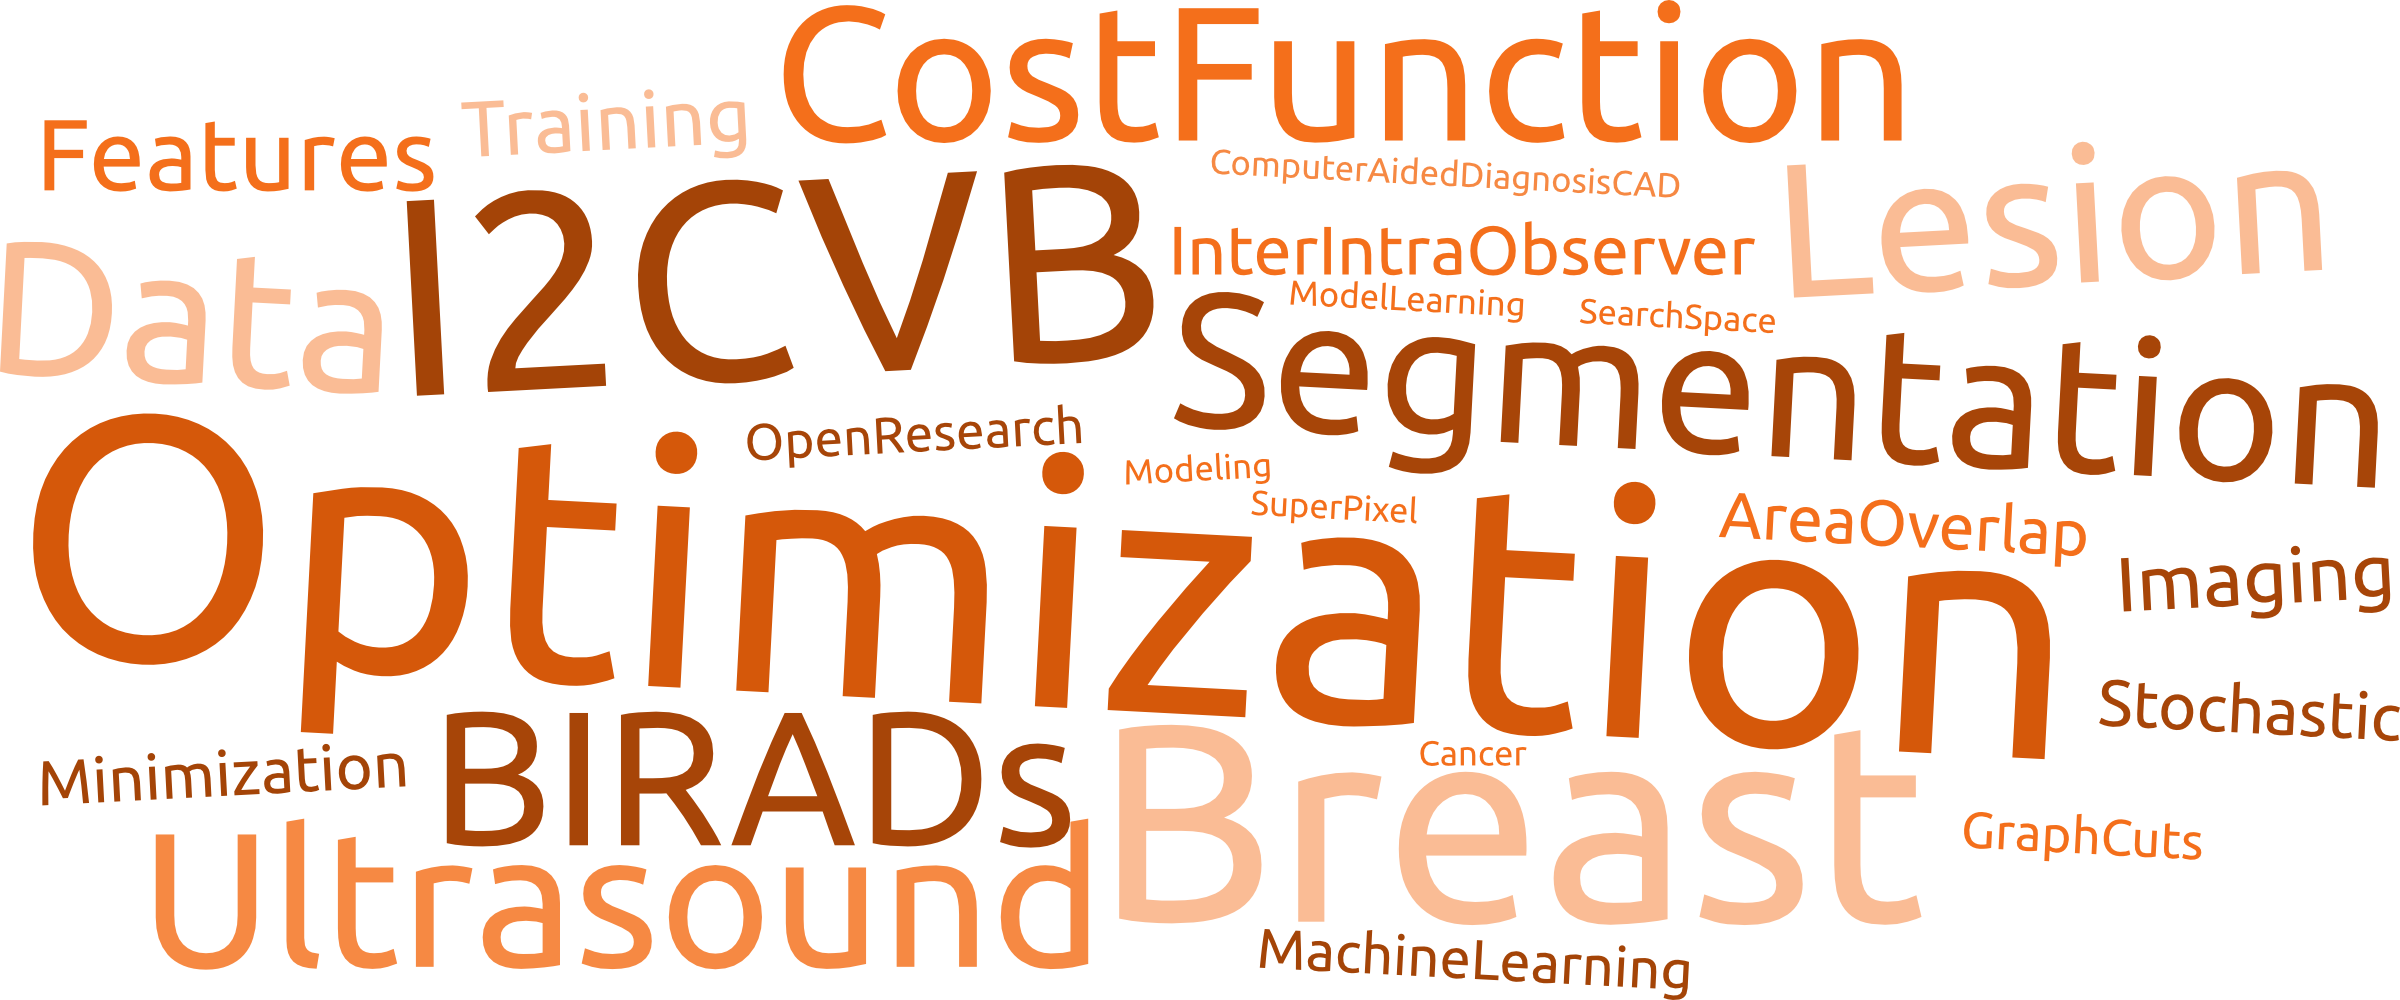
\includegraphics[width=.95\paperwidth]{orange_mix.png}};
    \end{tikzpicture}
  \end{beamercolorbox}
  % 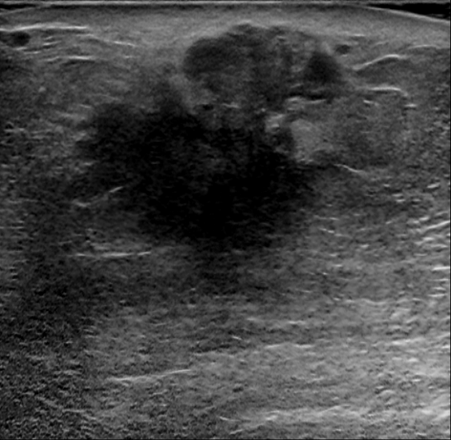
\includegraphics[trim=0 6 0 0,clip,height=.65\textheight]{a110105_094.png}~
\end{frame}


\begin{frame}[plain]{}
  \begin{beamercolorbox}[wd=\paperwidth,ht=\paperheight]{frametitle}
    \begin{tikzpicture}
      \fill[azulunam, opacity=1] (0, 0) rectangle(100, 100);
      \node [anchor=center] (cloud) at 
        (0.5\paperwidth, 0.5\paperheight)
        {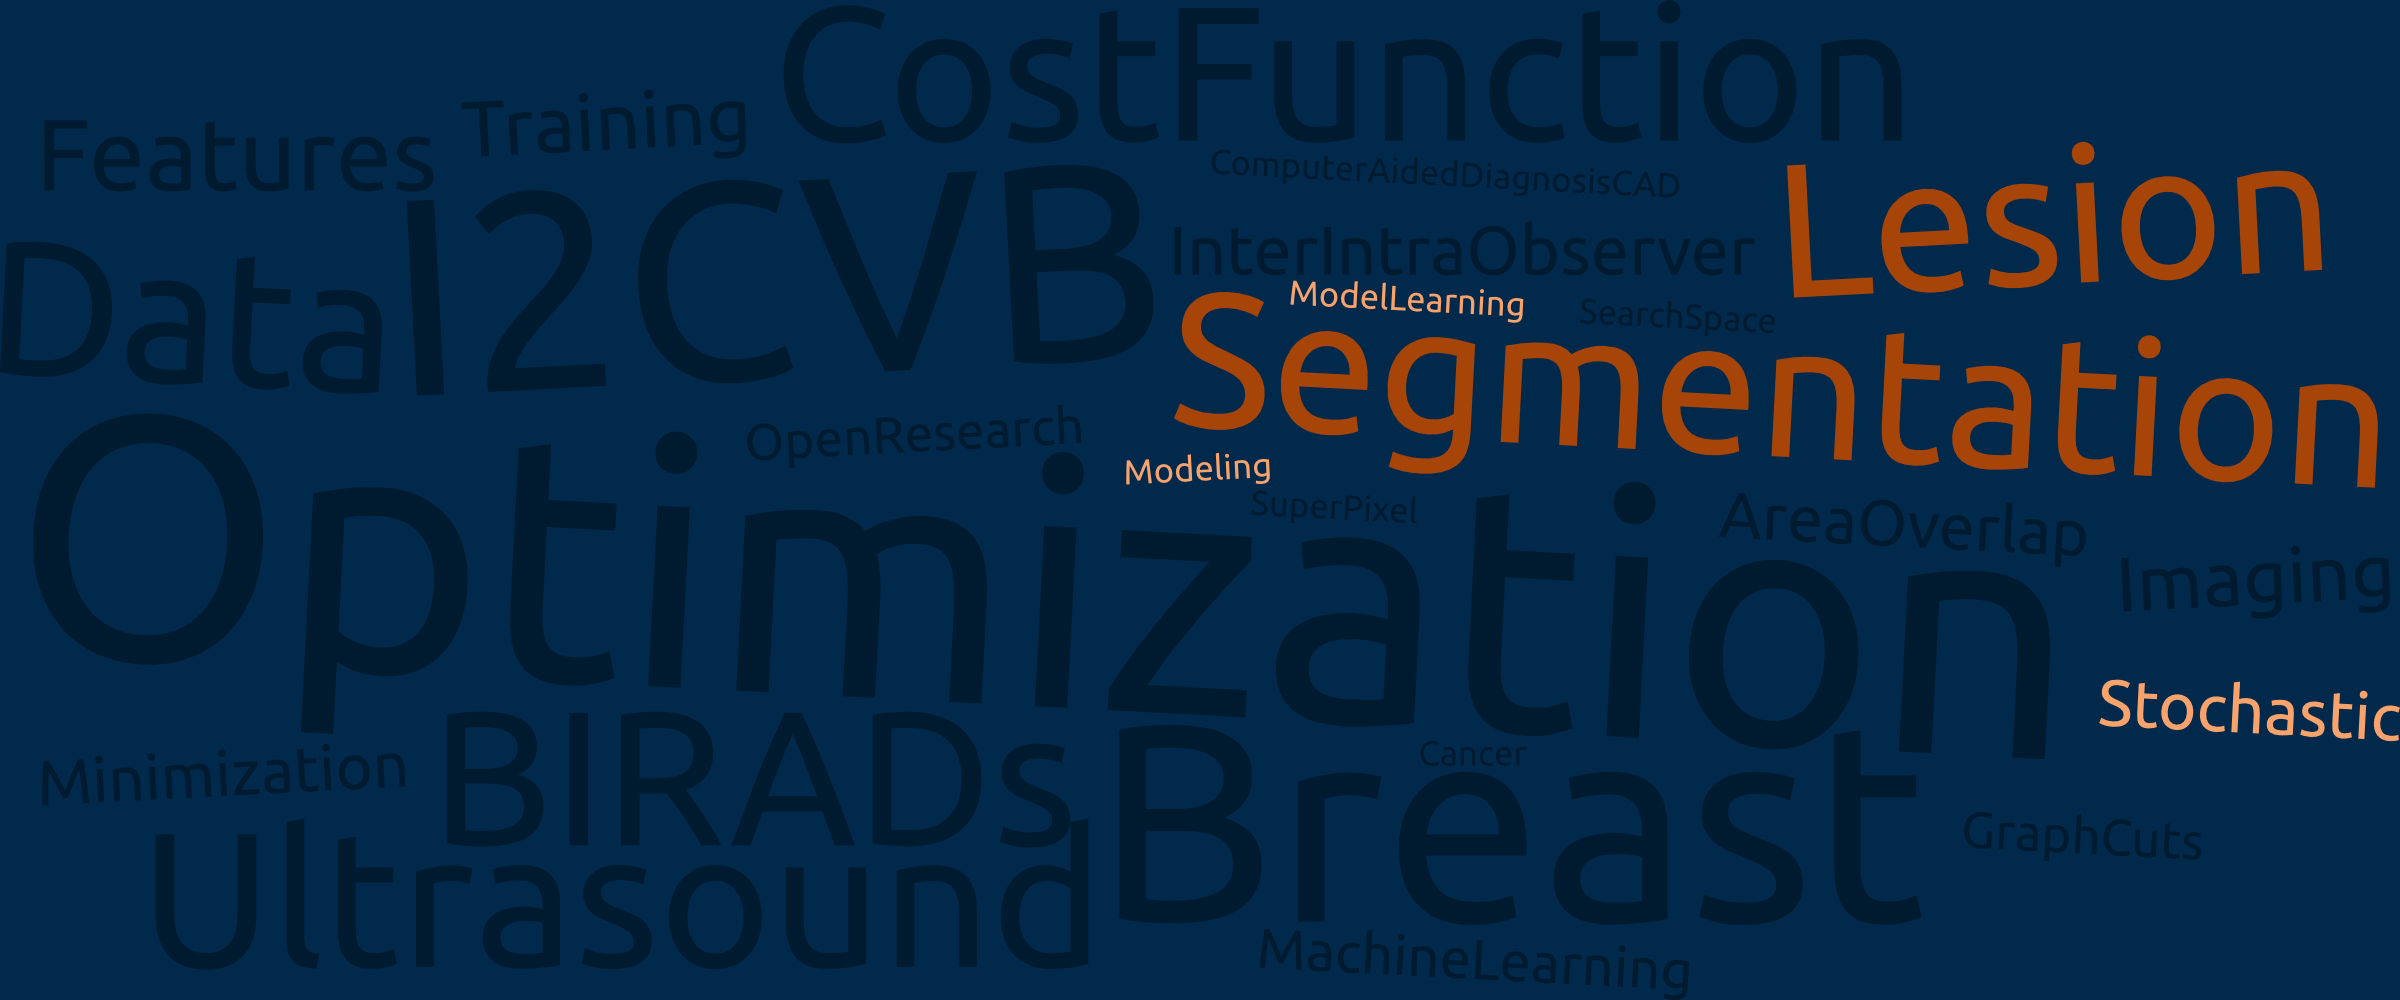
\includegraphics[width=.95\paperwidth]{highlight_prelude.png}};
    \end{tikzpicture}
  \end{beamercolorbox}
  % 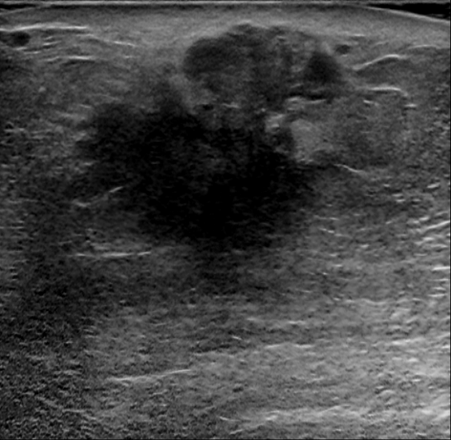
\includegraphics[trim=0 6 0 0,clip,height=.65\textheight]{a110105_094.png}~
\end{frame}

\begin{frame}[plain]\frametitle{Breast Lesion Segmentation in US images}
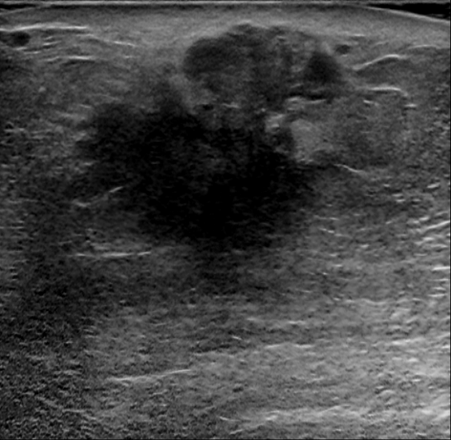
\includegraphics[trim=0 6 0 0,clip,height=.40\paperwidth]{a110105_094.png}~
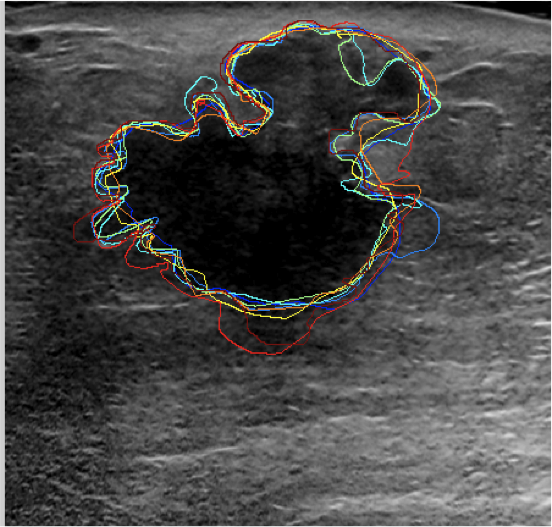
\includegraphics[trim=6 0 0 0,clip,height=.40\paperwidth]{segment.png}
\end{frame}



\begin{frame}
  \begin{beamercolorbox}[wd=\paperwidth,ht=\paperheight]{frametitle}
    \begin{tikzpicture}
      \fill[nicewhite, opacity=1] (0, 0) rectangle(1, 1);
      \node [anchor=center] (cloud) at 
        (0.5\paperwidth, 0.5\paperheight)
        {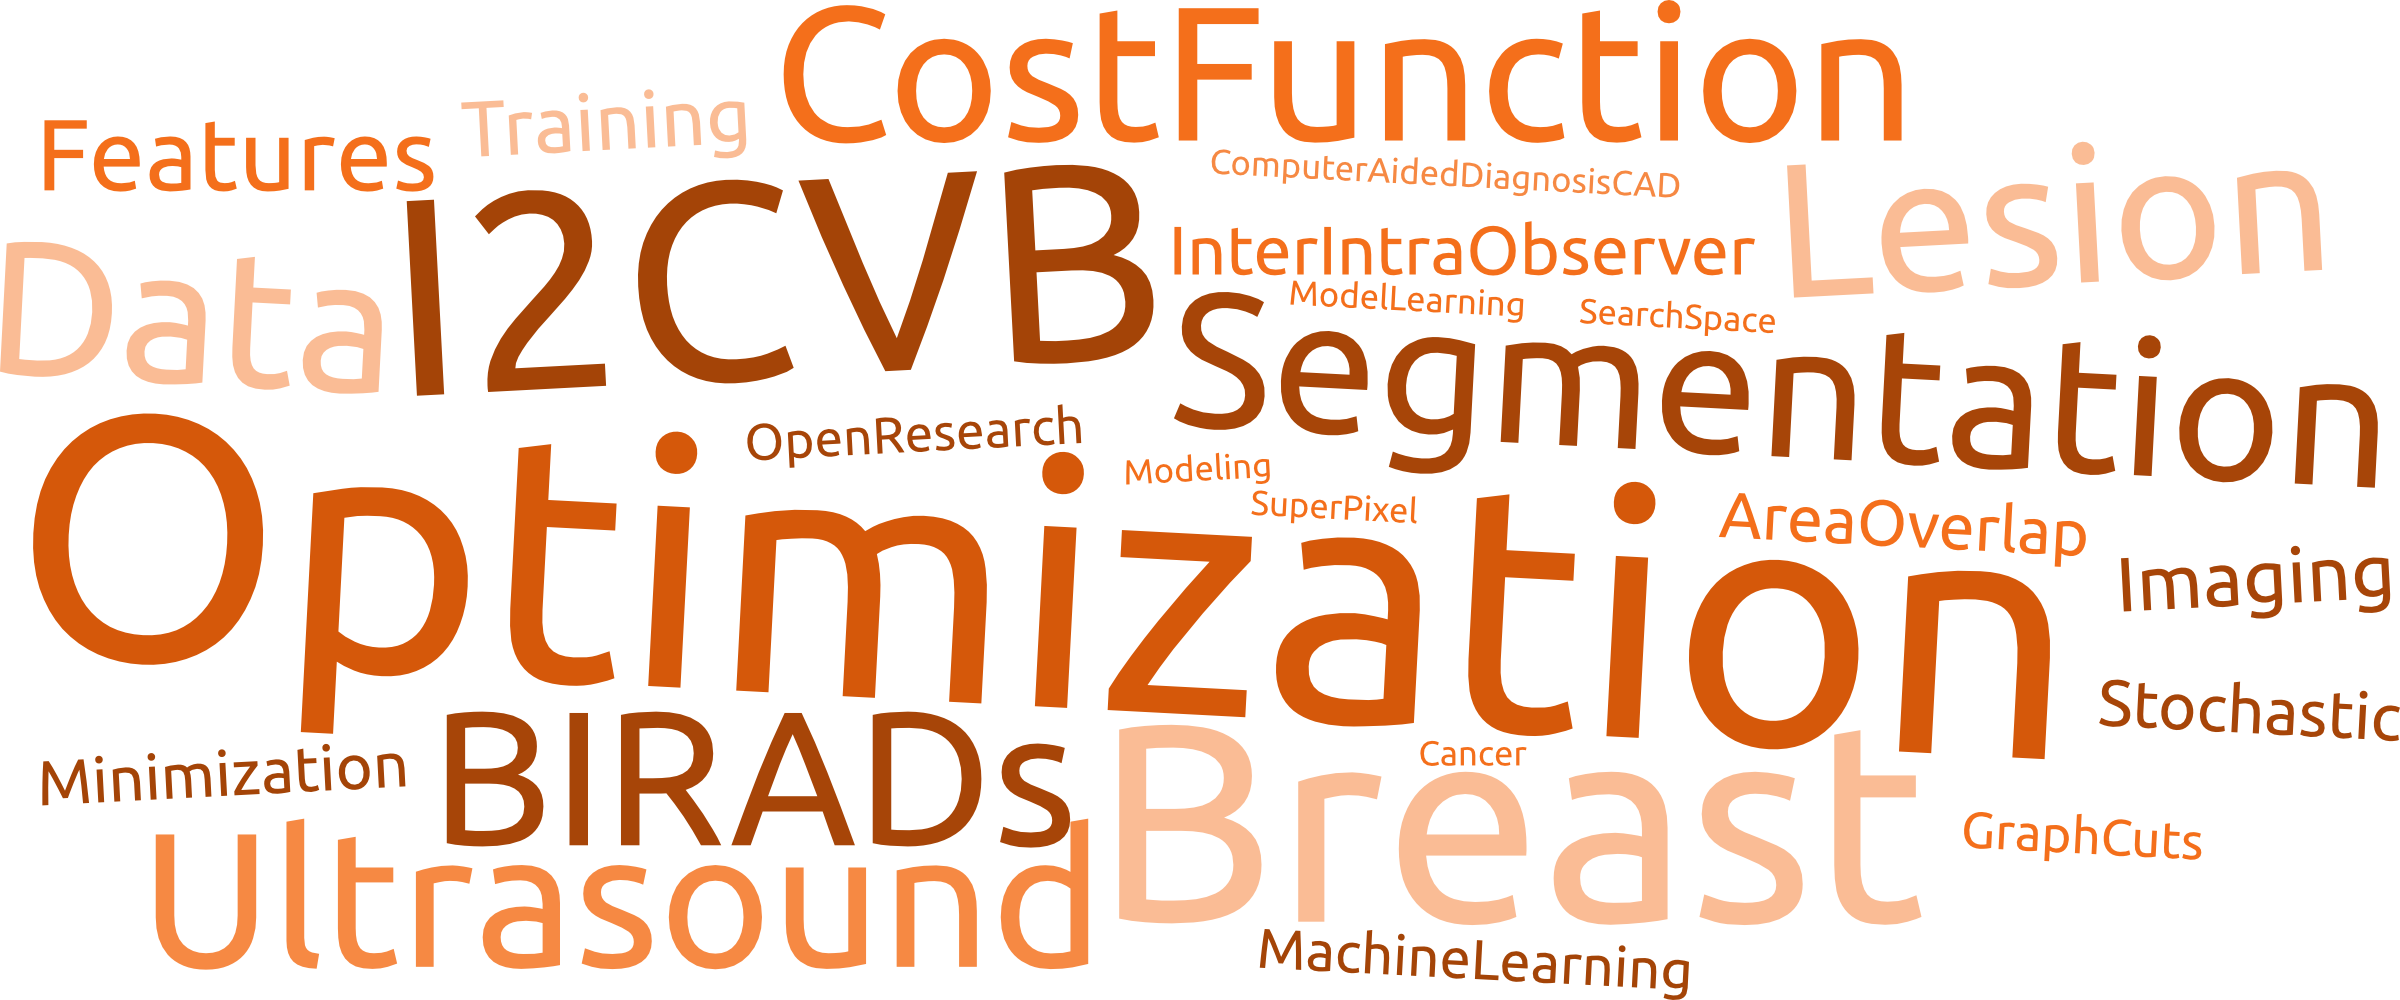
\includegraphics[width=.95\paperwidth]{orange_mix.png}};
    \end{tikzpicture}
  \end{beamercolorbox}
\end{frame}


\begin{frame}
  \begin{beamercolorbox}[wd=\paperwidth,ht=\paperheight]{frametitle}
    \begin{tikzpicture}
      \fill[nicewhite, opacity=1] (0, 0) rectangle(1, 1);
      \node [anchor=center] (cloud) at 
        (0.5\paperwidth, 0.5\paperheight)
        {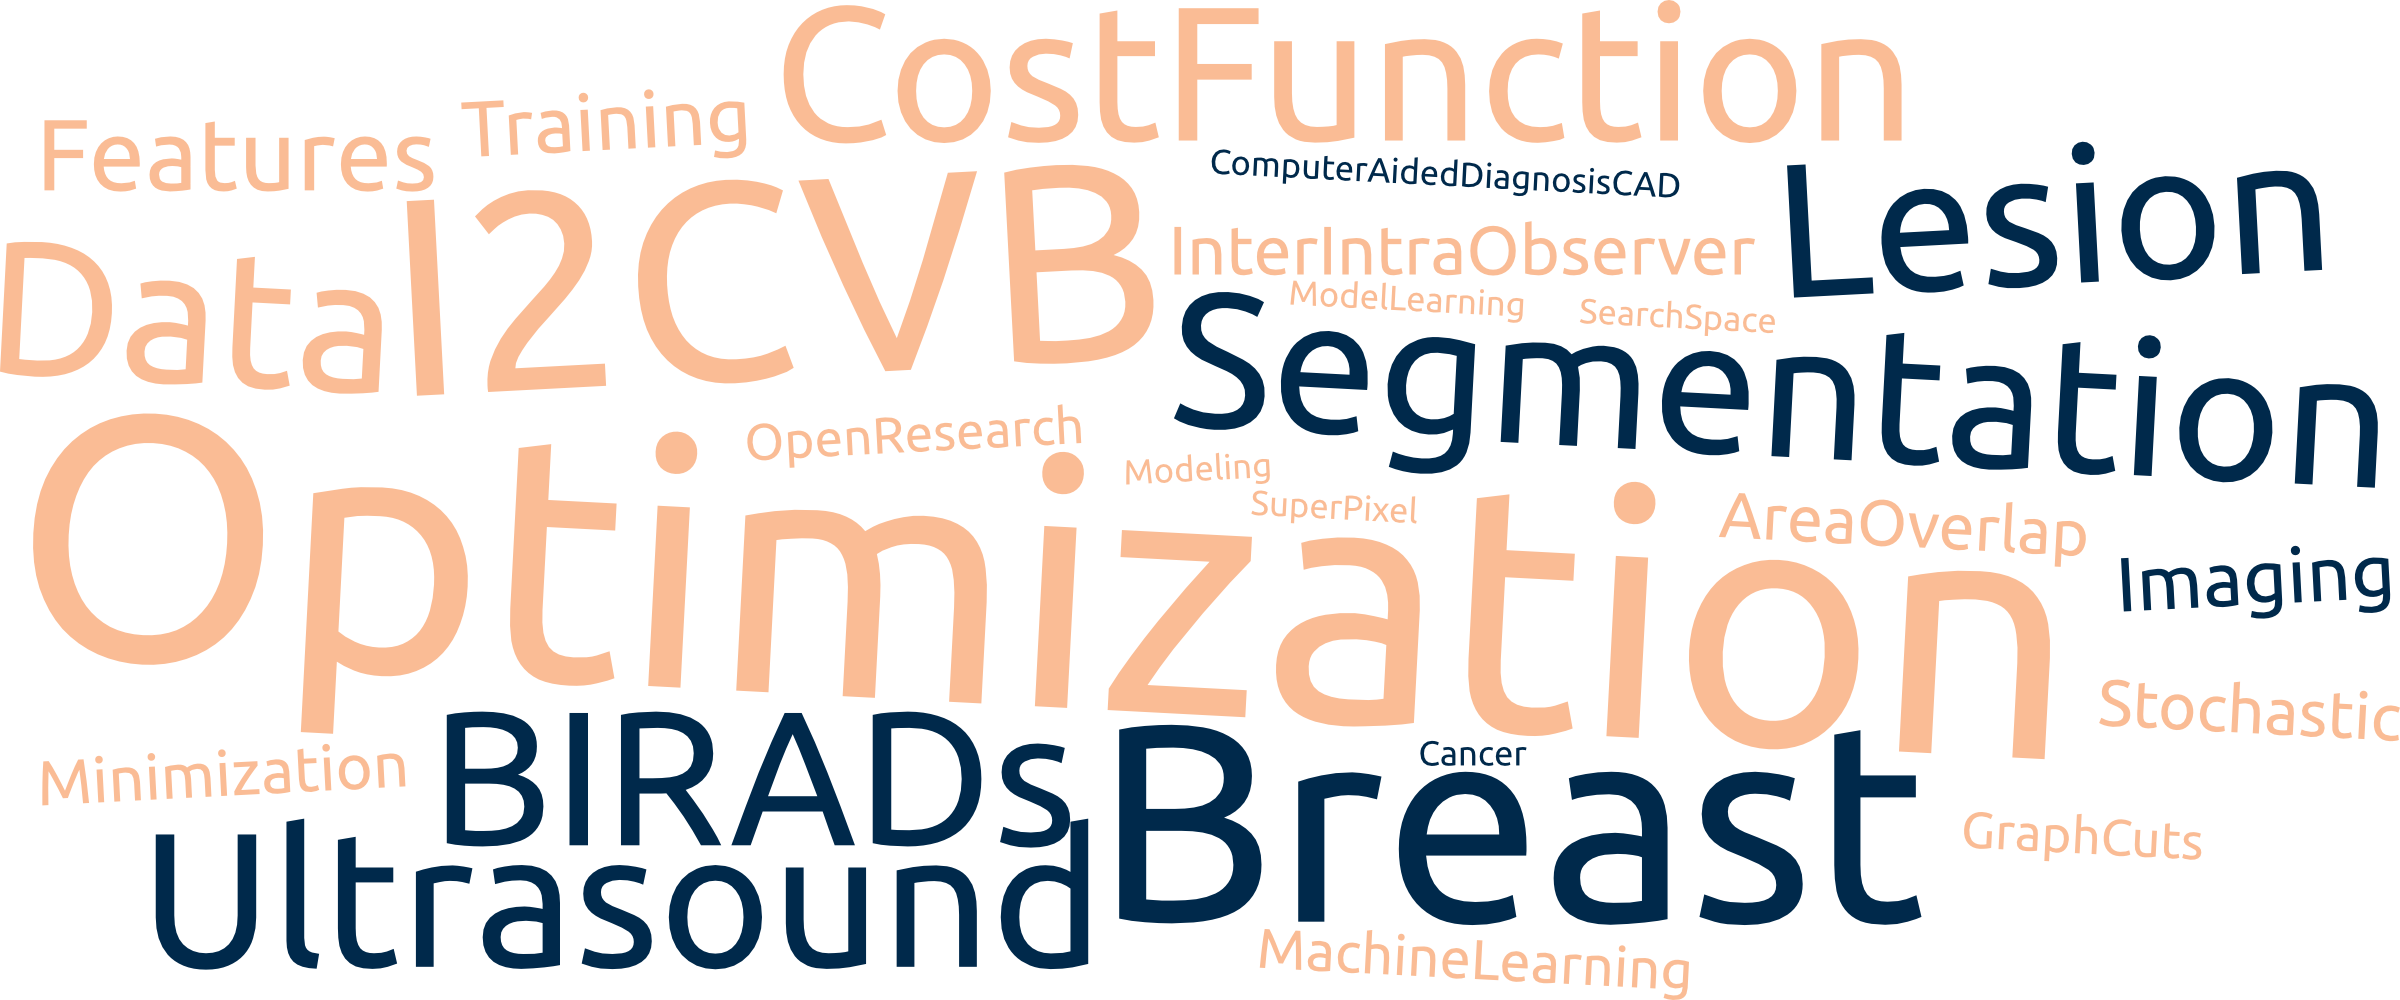
\includegraphics[width=.95\paperwidth]{intro.png}};
    \end{tikzpicture}
  \end{beamercolorbox}
\end{frame}


\begin{frame}
  \begin{beamercolorbox}[wd=\paperwidth,ht=\paperheight]{frametitle}
    \begin{tikzpicture}
      \fill[nicewhite, opacity=1] (0, 0) rectangle(1, 1);
      \node [anchor=center] (cloud) at 
        (0.5\paperwidth, 0.5\paperheight)
        {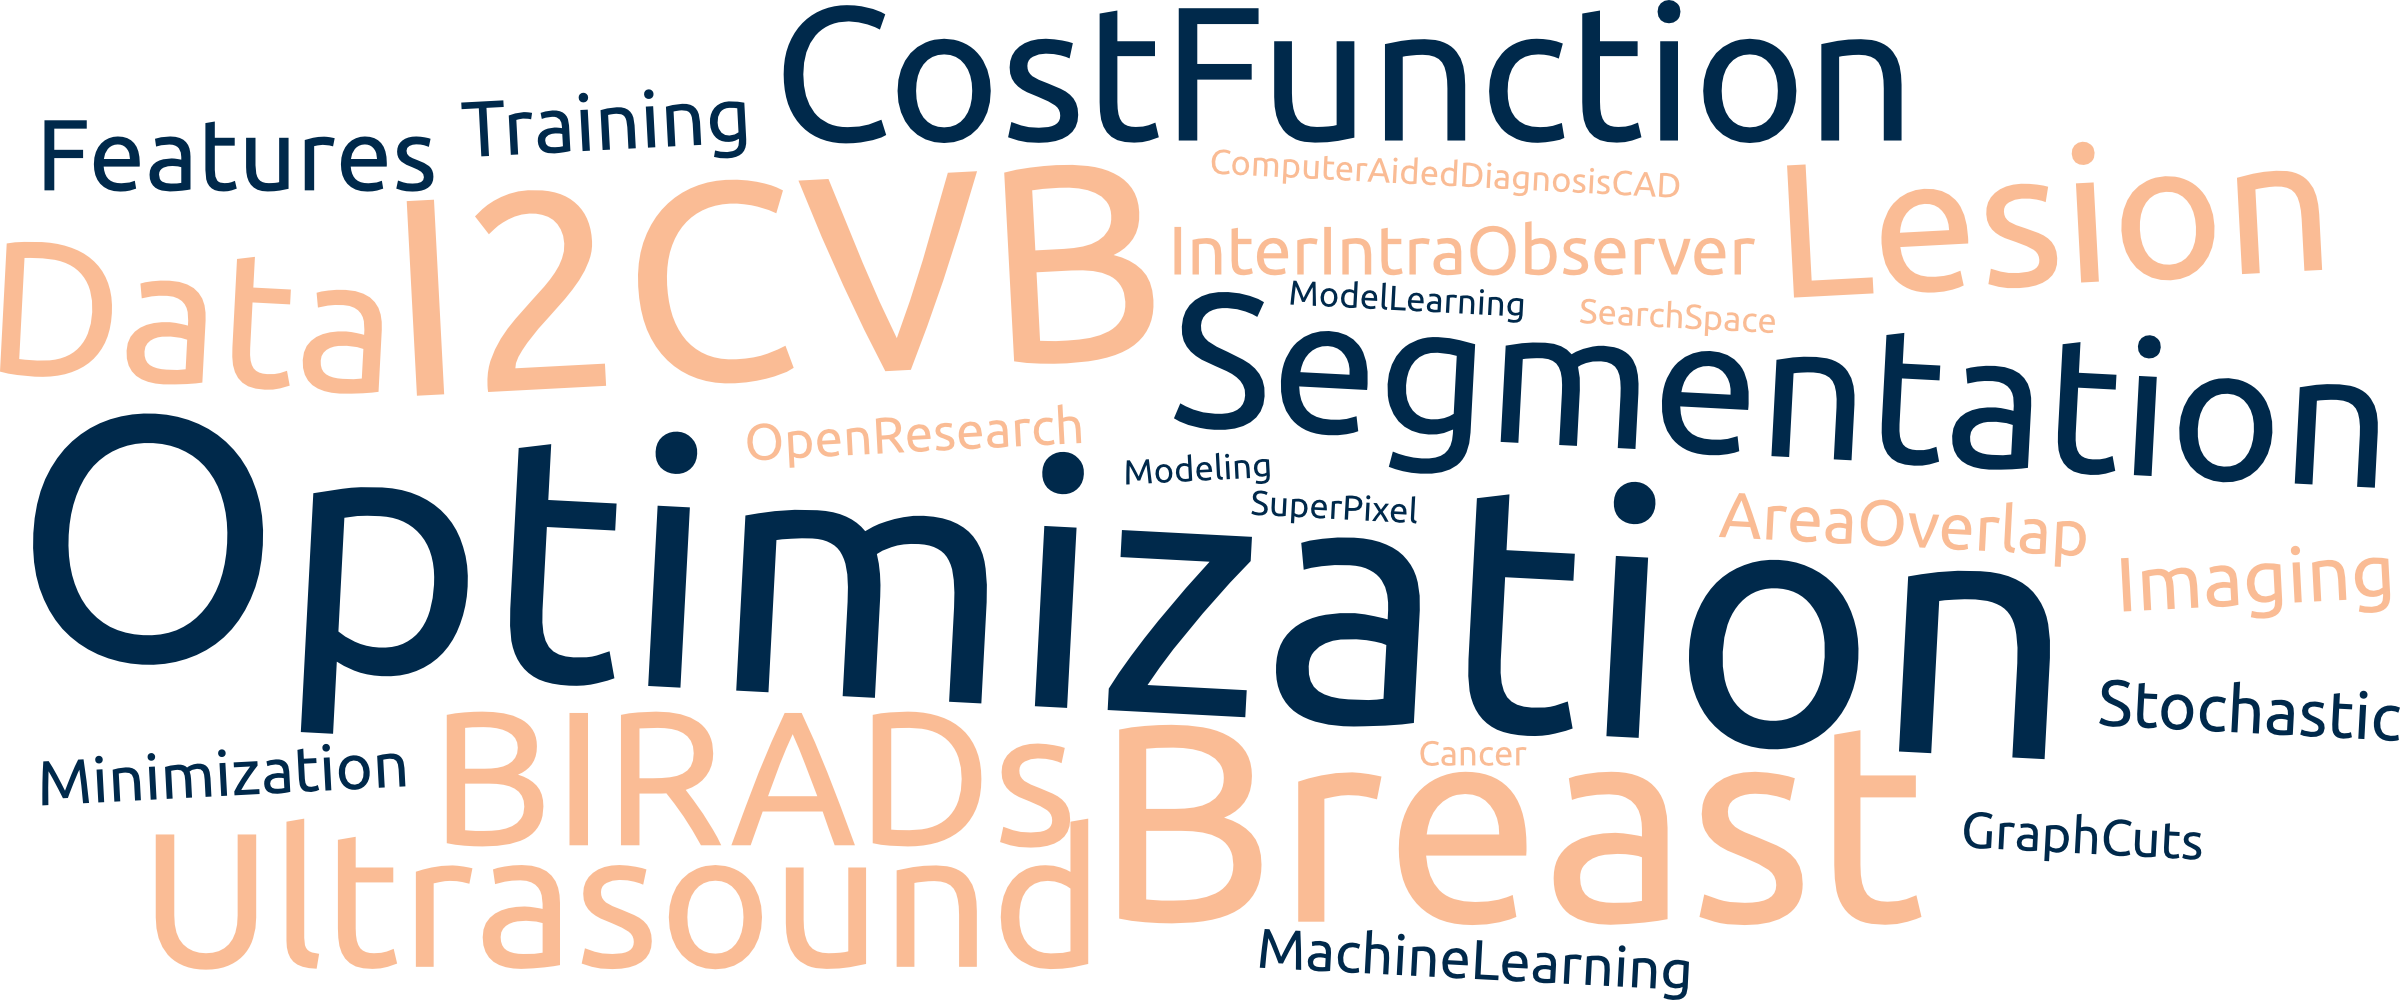
\includegraphics[width=.95\paperwidth]{method.png}};
    \end{tikzpicture}
  \end{beamercolorbox}
\end{frame}

\begin{frame}
  \begin{beamercolorbox}[wd=\paperwidth,ht=\paperheight]{frametitle}
    \begin{tikzpicture}
      \fill[nicewhite, opacity=1] (0, 0) rectangle(1, 1);
      \node [anchor=center] (cloud) at 
        (0.5\paperwidth, 0.5\paperheight)
        {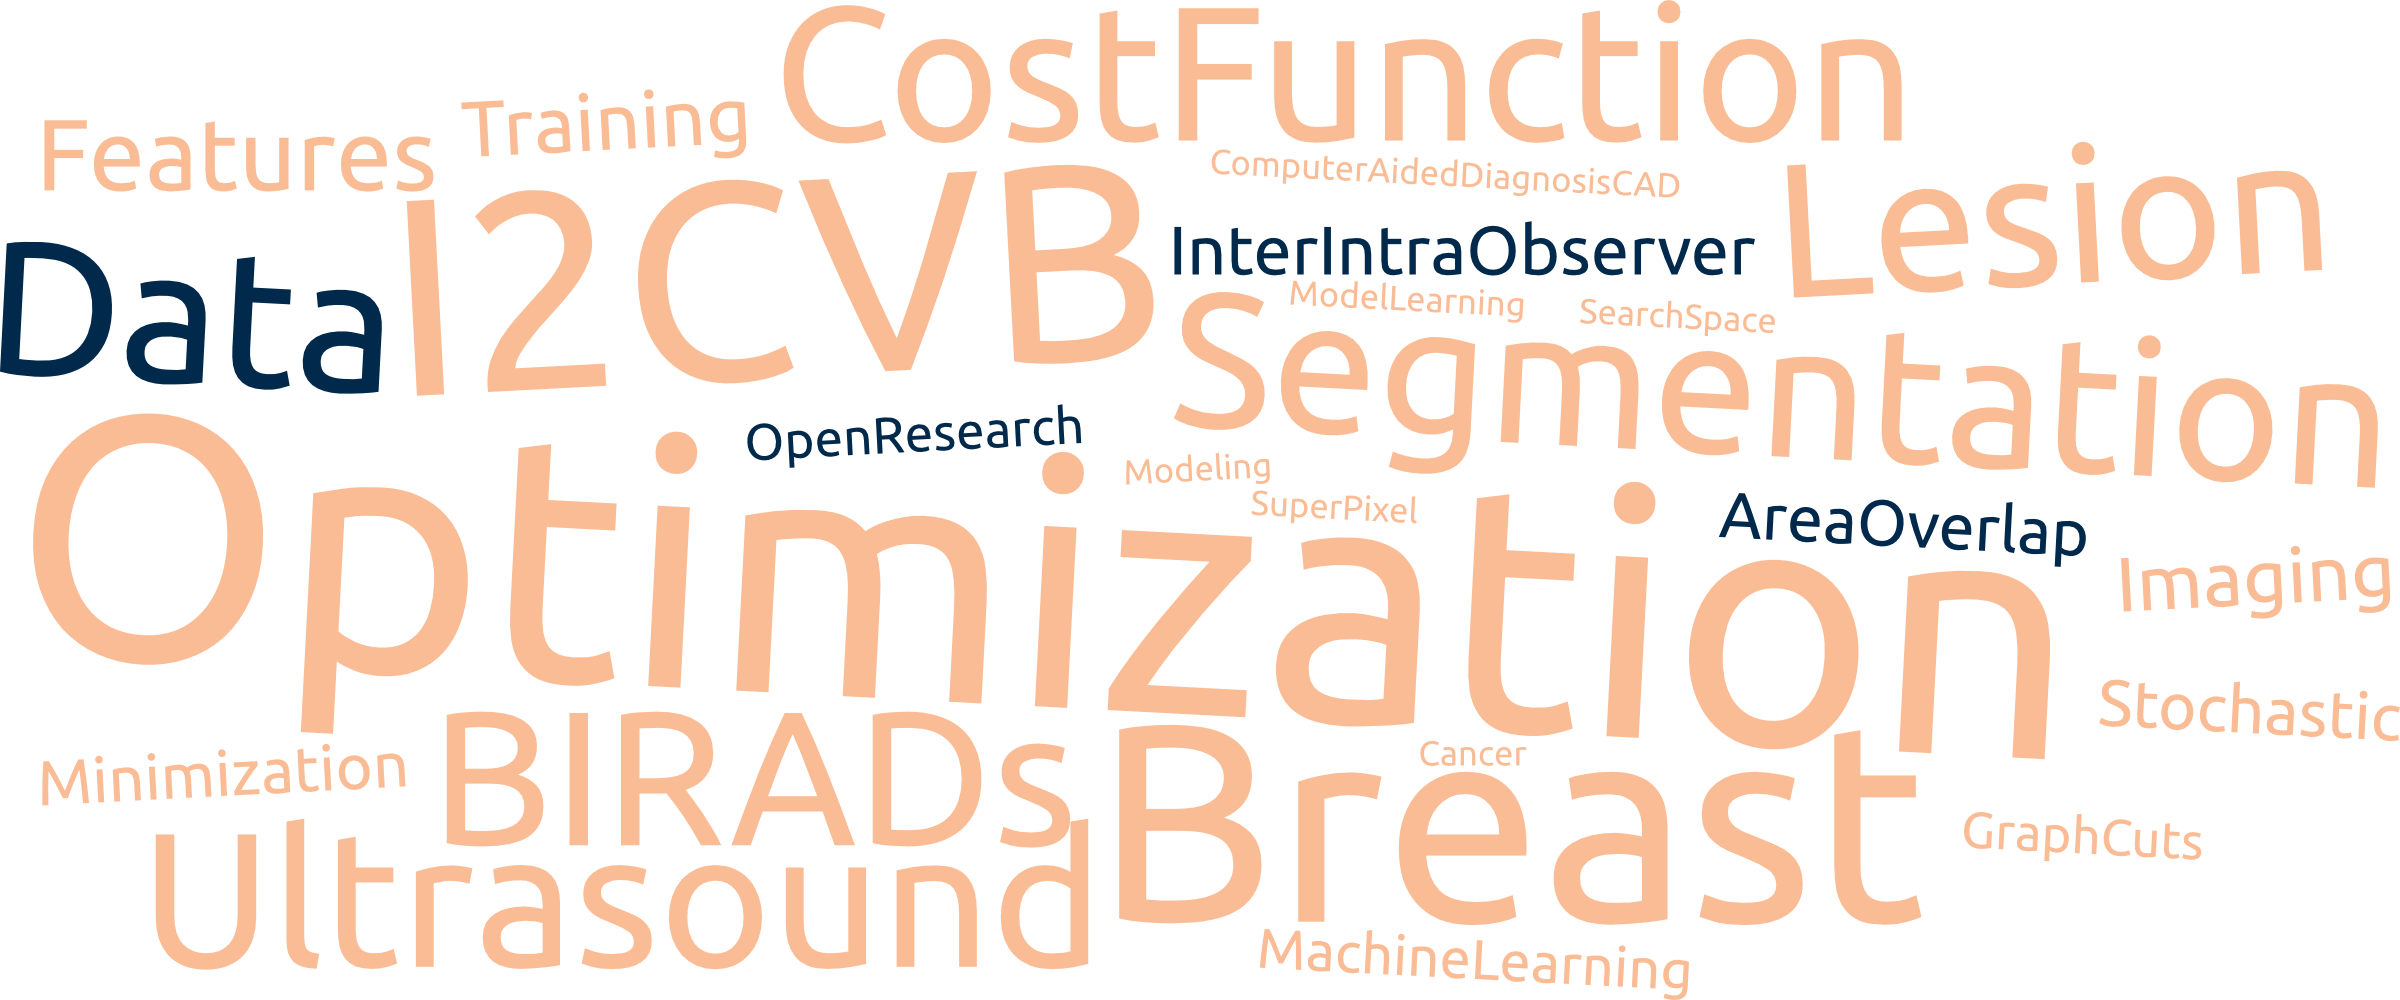
\includegraphics[width=.95\paperwidth]{results.png}};
    \end{tikzpicture}
  \end{beamercolorbox}
\end{frame}

\section{Introduction}
%\graphicspath{{chapters/introduction/figures/}}


\subsection{Motivations}

\begin{frame}{Motivations}
  % \frametitle{Introduction}
  % \framesubtitle{Motivations}
  \begin{block}{\small Statistics}
    \begin{figure}%
      \centering
      \hspace*{\fill}%
      \subfigure[][\tiny \# of cancer cases]{%
        \label{fig:stat1a}%
          \includegraphics[width=.45\textwidth]{./images/statistics/repartitionCancerIncidence.png}}%
      \hfill%
      \subfigure[][\tiny \# of cancer deaths]{%
        \label{fig:stat1b}%
          \includegraphics[width=.45\textwidth]{./images/statistics/repartitionCancerDeaths.png}}%
        \hspace*{\fill}%
      \label{fig:stat1}%
    \end{figure}
  \end{block}
  \begin{block}{\small Implications}\footnotesize
    \begin{itemize}
      \item 1.4 million cases per year
      \item 10.9\% of diagnosed cancers
      \item 5\textsuperscript{th} cause of cancer death
      \item 1\textsuperscript{th} cause of cancer death (females)
    \end{itemize}
  \end{block}
\end{frame}

\subsection{Screening}

\begin{frame}{Breast Imaging}
  % \frametitle{Introduction}
  % \framesubtitle{Screening}
  \begin{block}{\small Ultra-Sound(US) distinguishable lesion, shielded under Digital Mammography(DM)}\footnotesize
    \begin{figure}%
      \centering
      \hspace*{\fill}%
      \subfigure[][\tiny DM]{%
        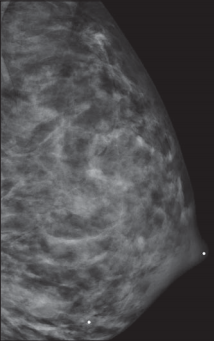
\includegraphics[trim = 0 0 0 20, clip,height=3.3cm]{mamo-us1.png}
        \label{fig:shielda}%
      \hfill%
      \subfigure[][\tiny DM, Region of Interest (ROI) ]{%
        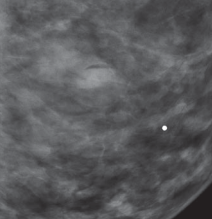
\includegraphics[trim = 0 0 0 20, clip,height=3.3cm]{mamo-us2.png}
        \label{fig:shieldb}%
      \hfill%
      \subfigure[][\tiny Breast Ultra-Sound(BUS), ROI]{%
        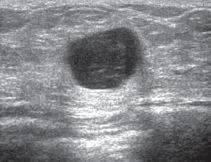
\includegraphics[trim = 10 20 10 0, clip,height=3.3cm]{mamo-us3.png}
        \label{fig:shieldc}%
        \hspace*{\fill}%
      \label{fig:shield}%
    \end{figure}
  \end{block}

  \begin{block}{\small US imaging as adjunct image modality}\footnotesize
    \begin{itemize}
    \item Most common adjunct image modality
    \item Ability to discern solid lesions typologies
    \end{itemize}
  \end{block}

\end{frame}

\subsection{Image formation, limitations and imaging perspectives}
\begin{frame}\frametitle{Breast structures and appearance under US screening}
\begin{columns}
\begin{column}{.48\textwidth}\vspace{-17pt}%\hspace{-1cm}
\begin{figure}\centering
\begin{tikzpicture}[scale=.5]
\begin{scriptsize}
	\tikzset{dot/.style={circle,draw=black,inner sep=0mm,minimum size=4pt}}
    \node[anchor=south west,inner sep=0] at (.2,.2) {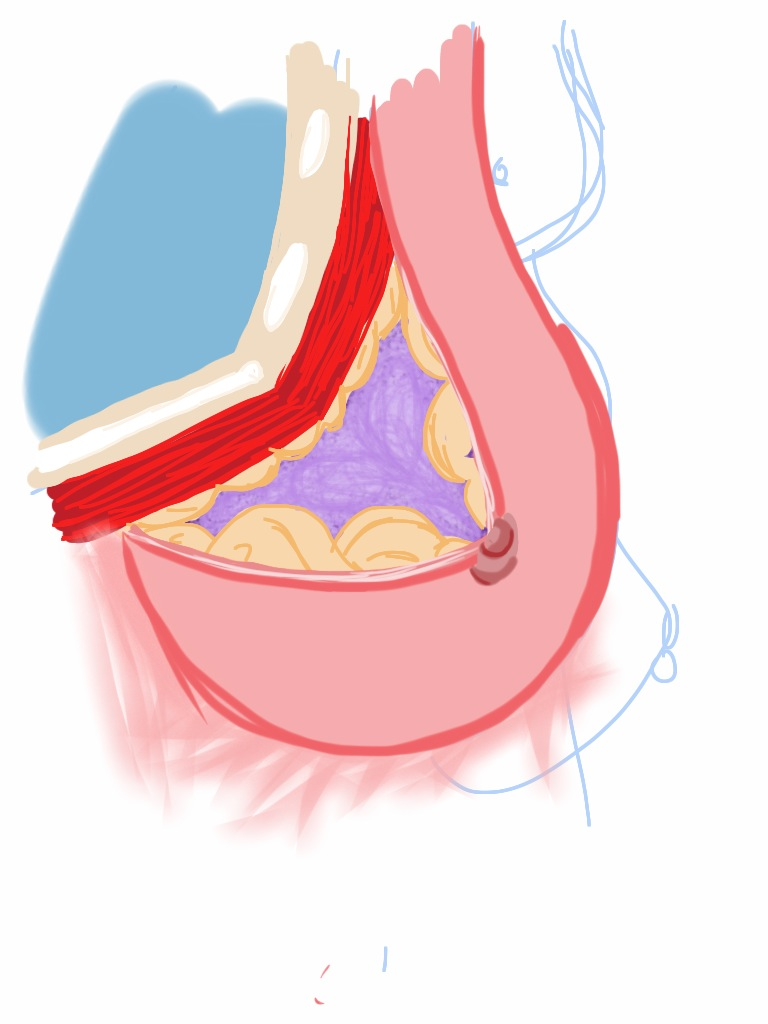
\includegraphics[trim = 20 190 80 20, clip,height=\textwidth]{pit.jpg}};
    \draw		(1.75,	7.75	) 	node[dot]	(AirCoord)			{}	
    				(2.5	,	5		) 	node[dot]	(PecCoord)			{}
    				(3.75,  7.75	) 	node[dot]	(CWCoord)			{}
    				(5,		5.40	) 	node[dot]	(TissueCoord)	{}
    				(2.5	,	3.65	) 	node[dot]	(SkinCoord)		{}
    				(3.75, 3.8	)  	node[dot]	(CooperCoord)	{}
    				(5.80, 5.40	)  	node[dot]	(FatCoord)			{};
 	   				
\draw	(AirCoord)	node[above left] (AirName) {Lungs (air)}
			node[below =of AirName.west, anchor=west] (PecName){Pectoral muscle}
   			(4.5,9.5)	node[anchor=west] (CWName){Chest-wall}
			node[below = of CWName,anchor=west,text width=2cm] (TissueName){Fibro-glandular tissue}
%    			(SkinCoord)
    			node[below= 1.8 of PecName.west, anchor=west ] (SkinName){Skin layers}
    			(CooperCoord |- SkinName)	node[text width=1.5cm,anchor= north west,inner sep=0mm,xshift=-5pt] (CooperName){Cooper's ligament}
    			(FatCoord) node[xshift=9,inner sep=0mm,anchor=west,text width=2cm] (FatName){Adipose tissue \emph{fat lobe}}
;   					 	
    \draw 	(PecCoord) -- (PecName)
    		   	(SkinCoord) -- (SkinName) 
				(CooperCoord) -- (CooperName)
%				(AirCoord) -- (AirName.south)
				(CWCoord) -- (CWName)
				(TissueCoord) -- (TissueName.west)
				(FatCoord) -- (FatName)
				;
%    
%    \draw[help lines,xstep=.5,ystep=.5] (0,0) grid (10,10);
%\foreach \x in {0,1,...,10} { \node [anchor=north] at (\x,0) {\x}; }
%\foreach \y in {0,1,...,10} { \node [anchor=east] at (0,\y) {\y}; });
\end{scriptsize}
\end{tikzpicture}
		\caption{Breast structure elements.}
		\end{figure}	
\end{column}

\begin{column}{.48\textwidth}
\begin{overprint}
\onslide<1|handout:0>
\begin{figure}
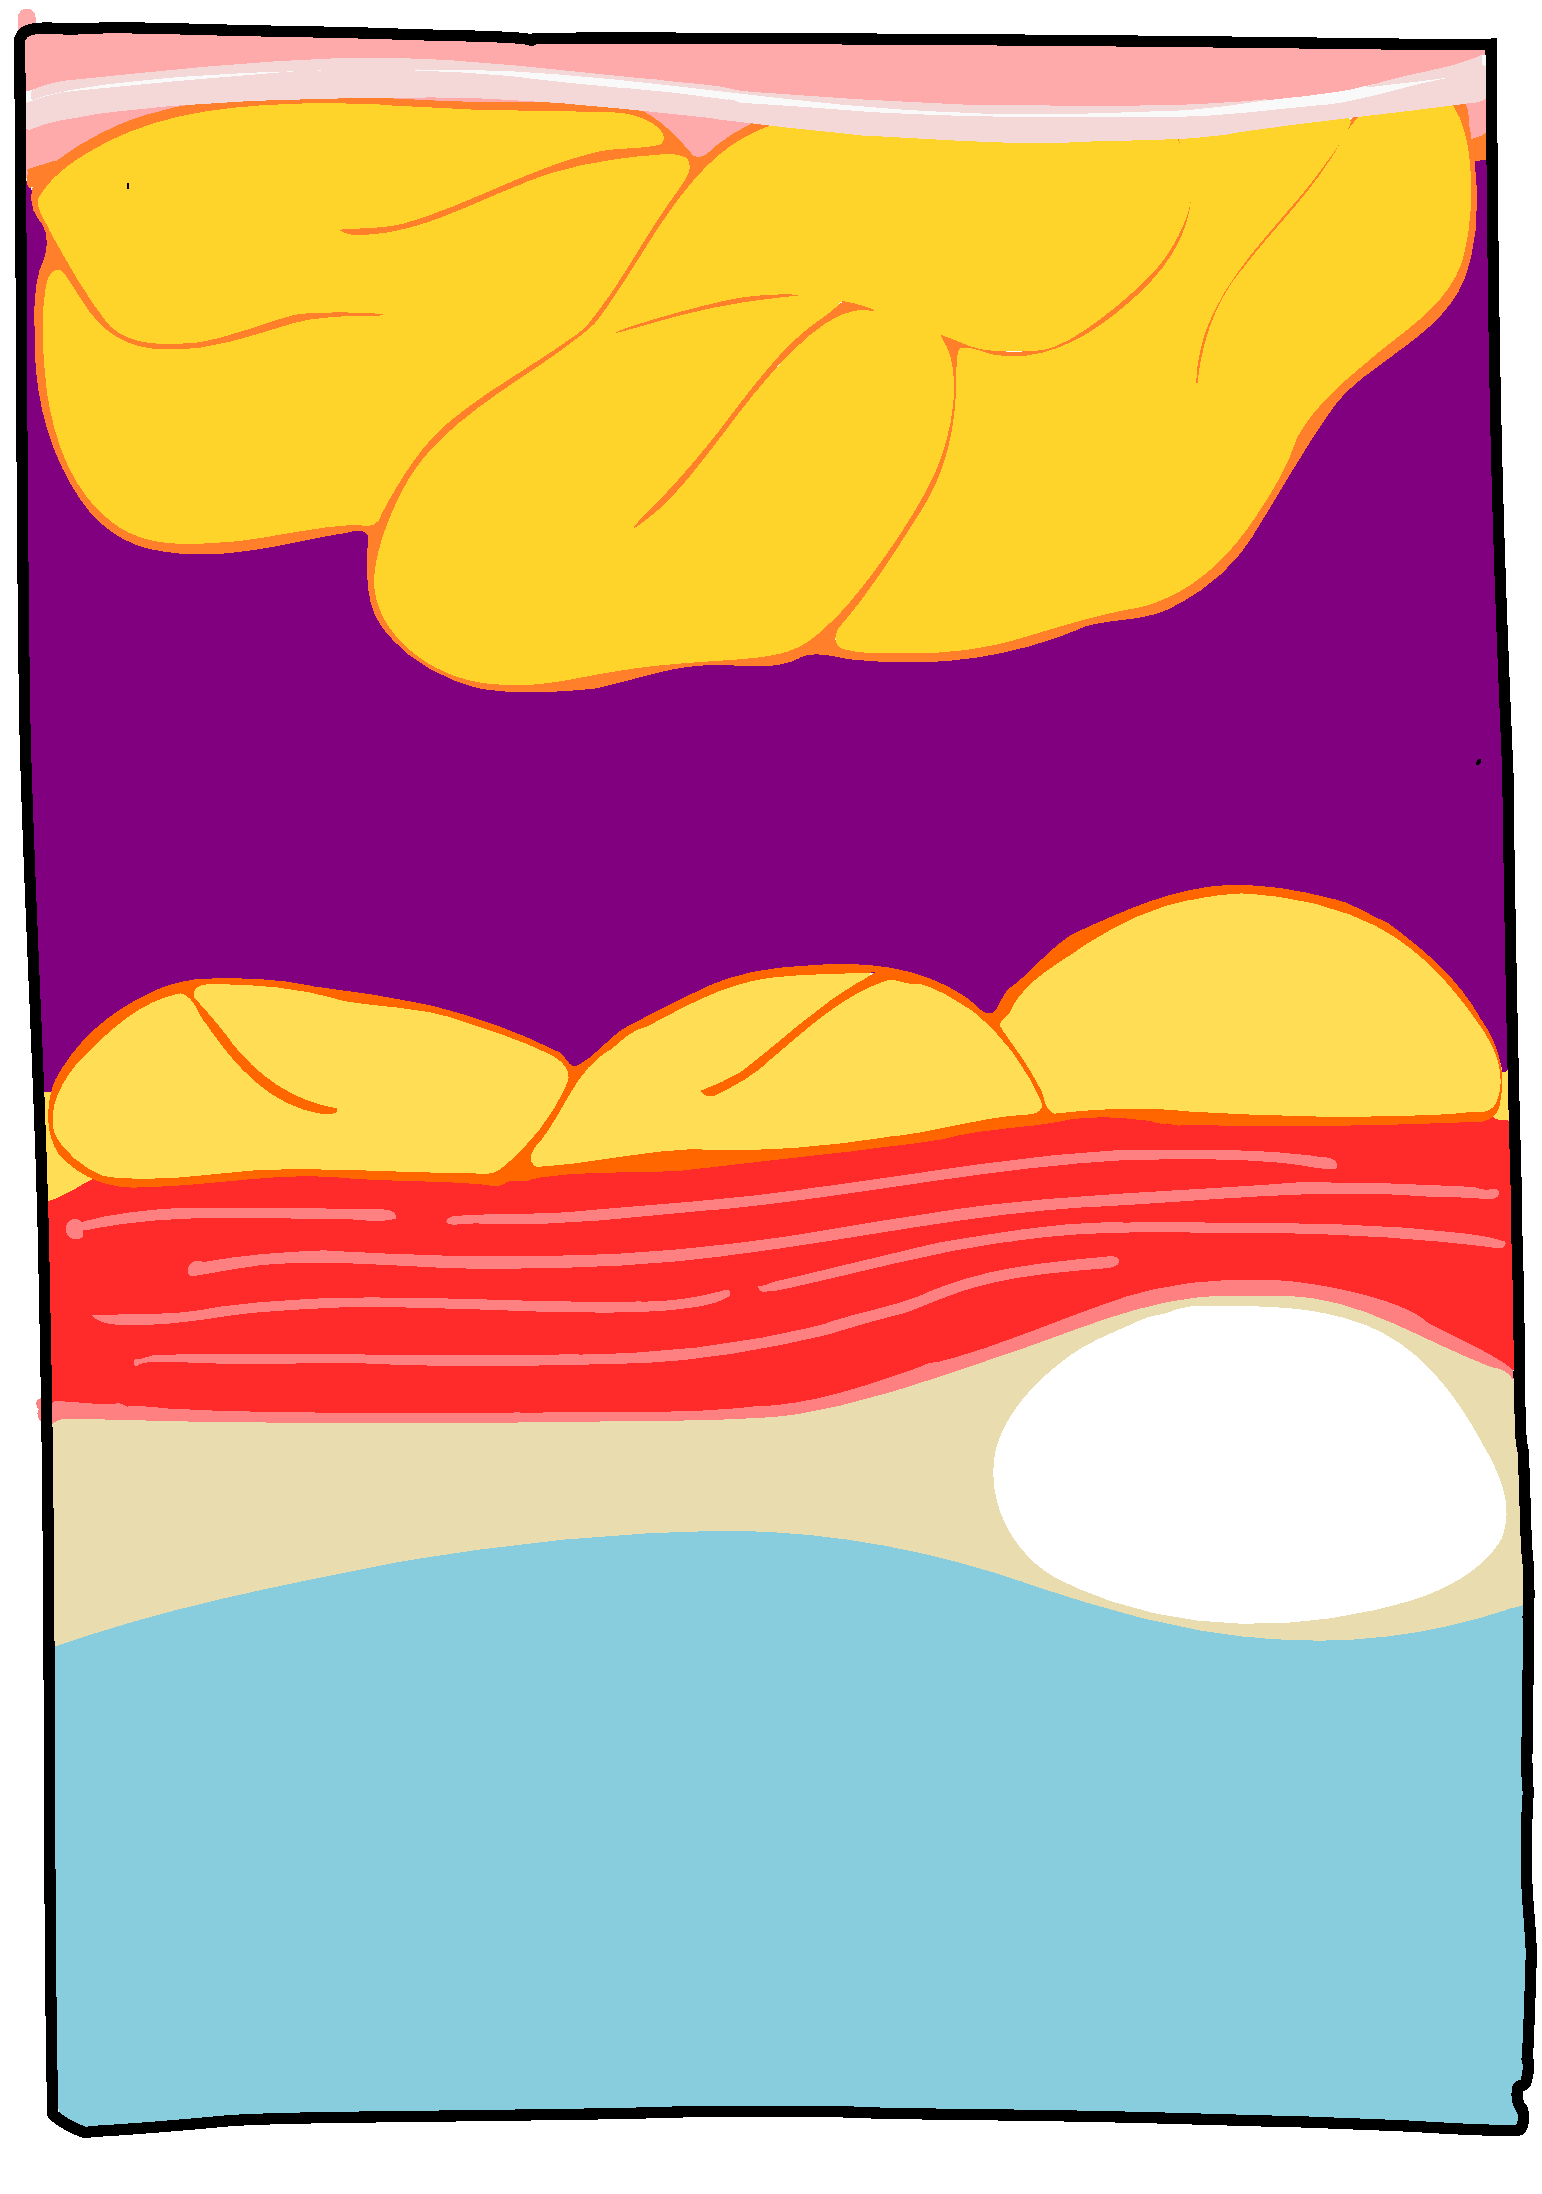
\includegraphics[width=.7\textwidth]{slice/tissue.pdf}
\caption{ Scheme of the elements present in a Breast \ac{us} image.}
		\end{figure}	
		
\onslide<2|handout:0>
		\begin{figure}
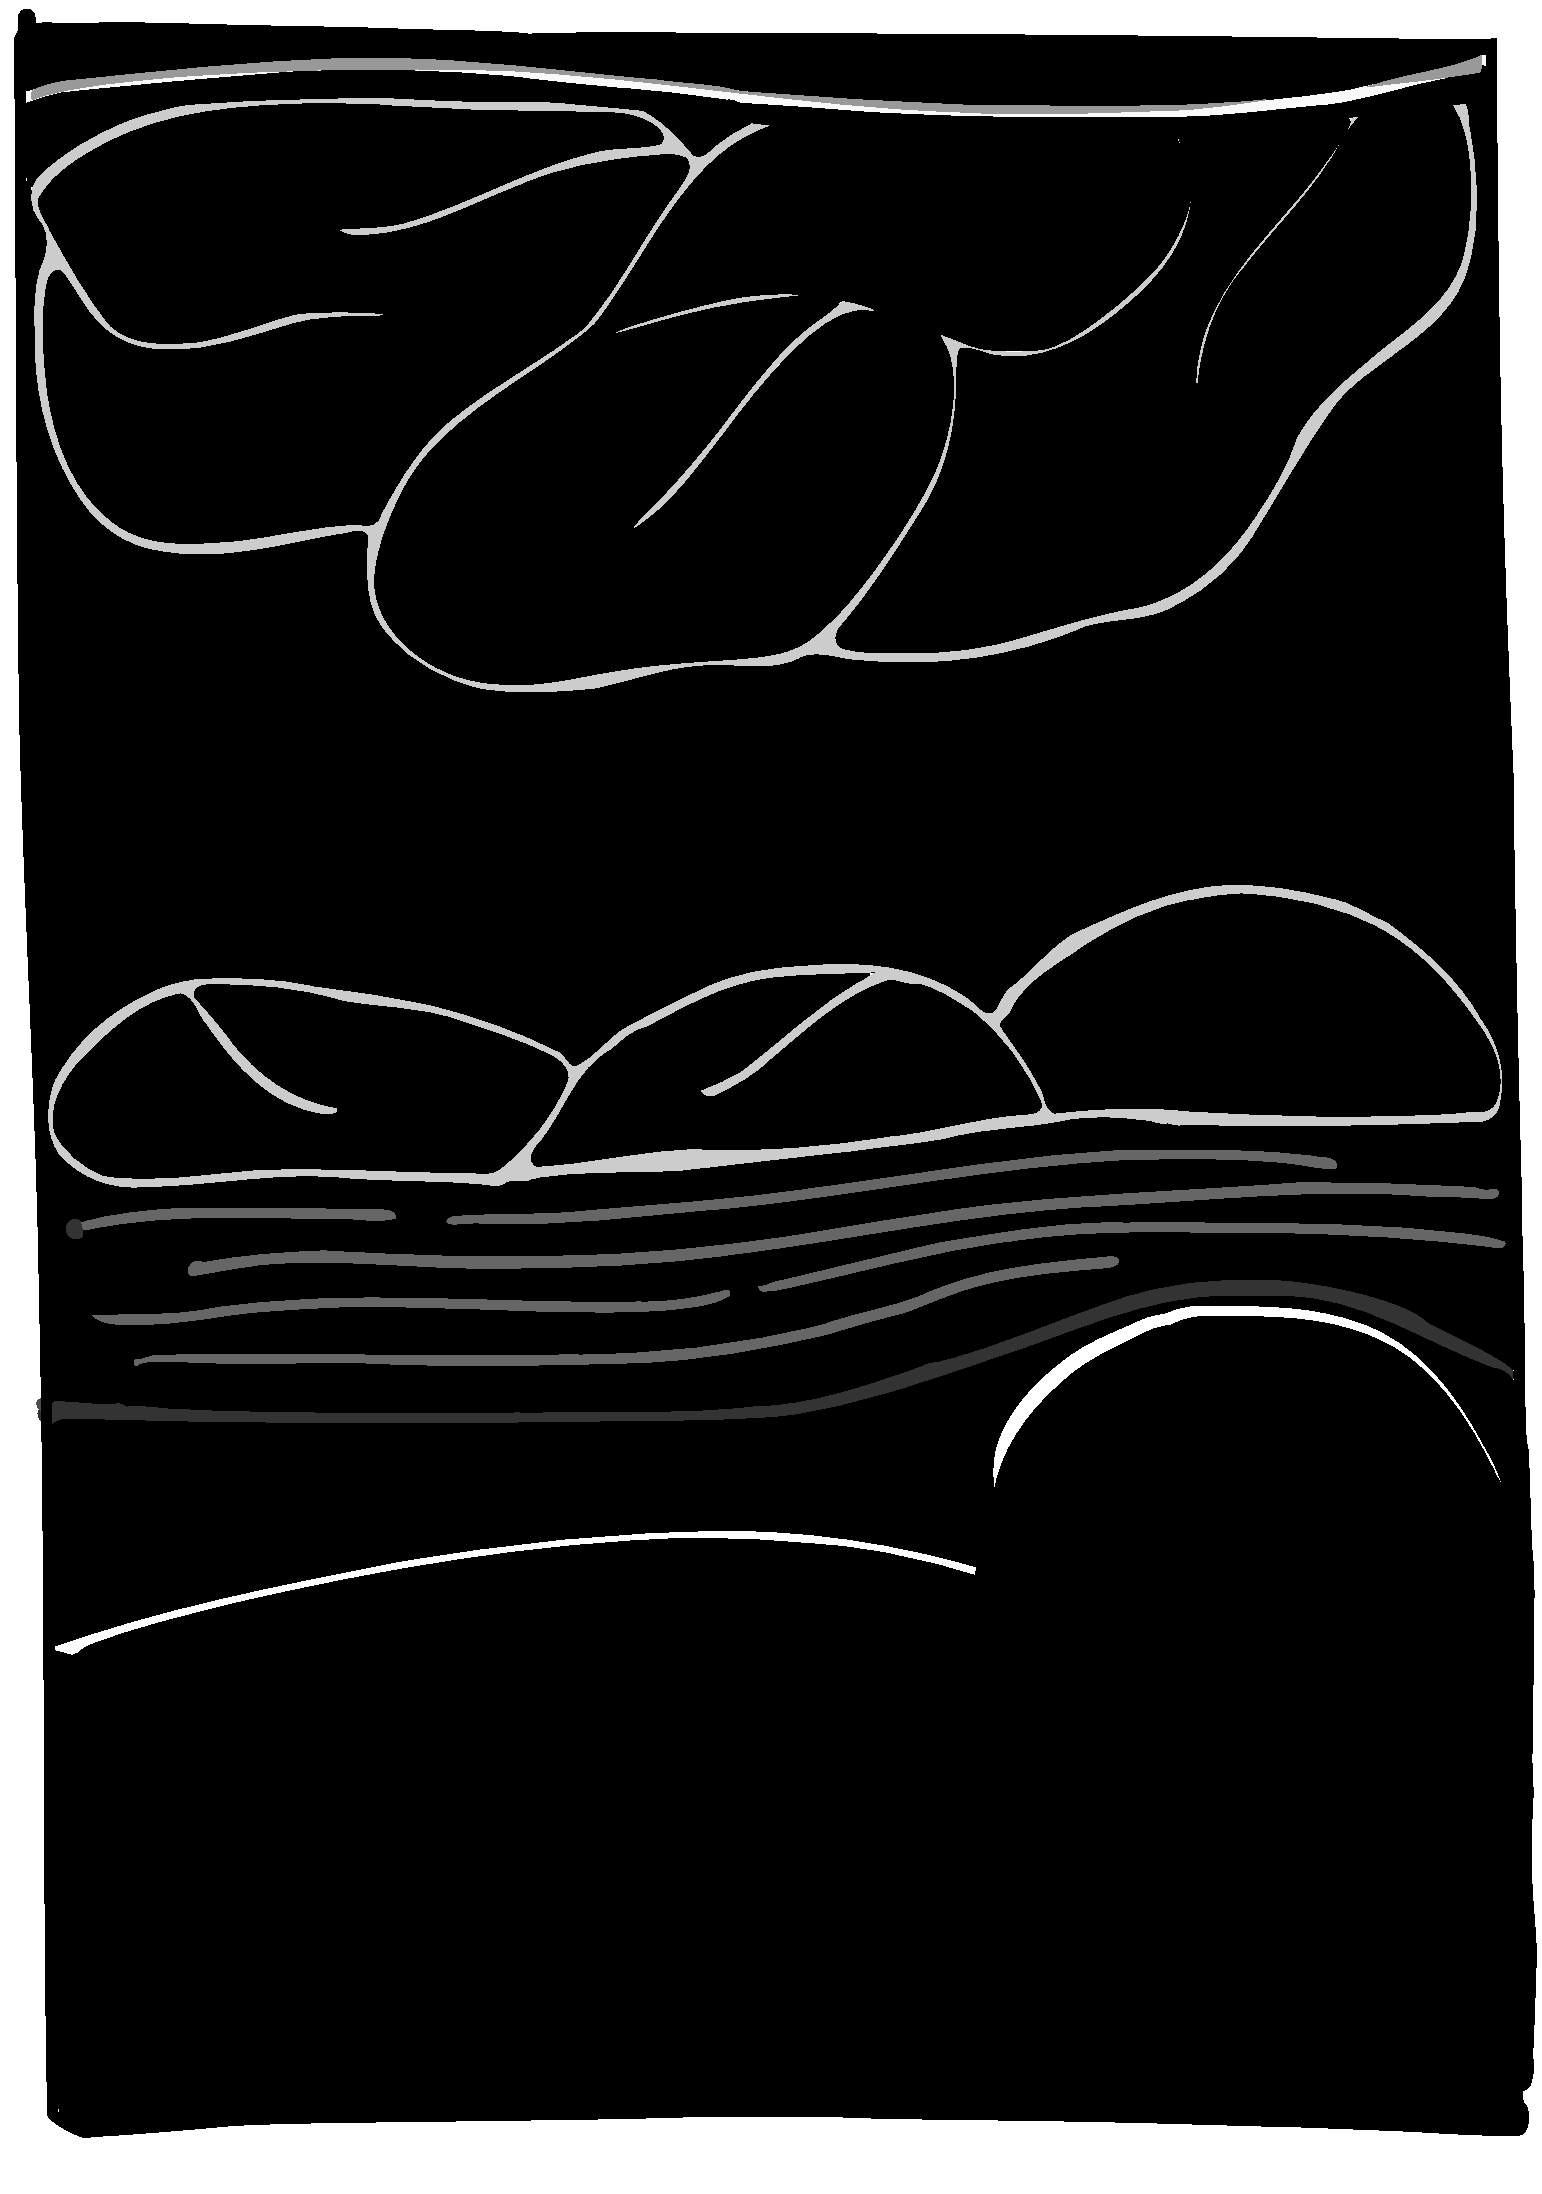
\includegraphics[width=.7\textwidth]{slice/US.pdf}
	\caption{Ideal Breast \ac{us} screening based on depicting the reflection produced on the different tissue boundaries.}
		\end{figure}	
\end{overprint}
\end{column}
\end{columns}
\end{frame}

\begin{frame}\frametitle{Breast structures and appearance under US screening}
%This slide needs to be parted into two slides or a dinamic one where first is olny analyzed specular reflection and seond the scattering.
\begin{columns}
\begin{column}{.48\textwidth}\hspace{-1cm}
\begin{tikzpicture}[scale=1]
\begin{scriptsize}
	 \node[anchor=south west,inner sep=0] at (0,0) {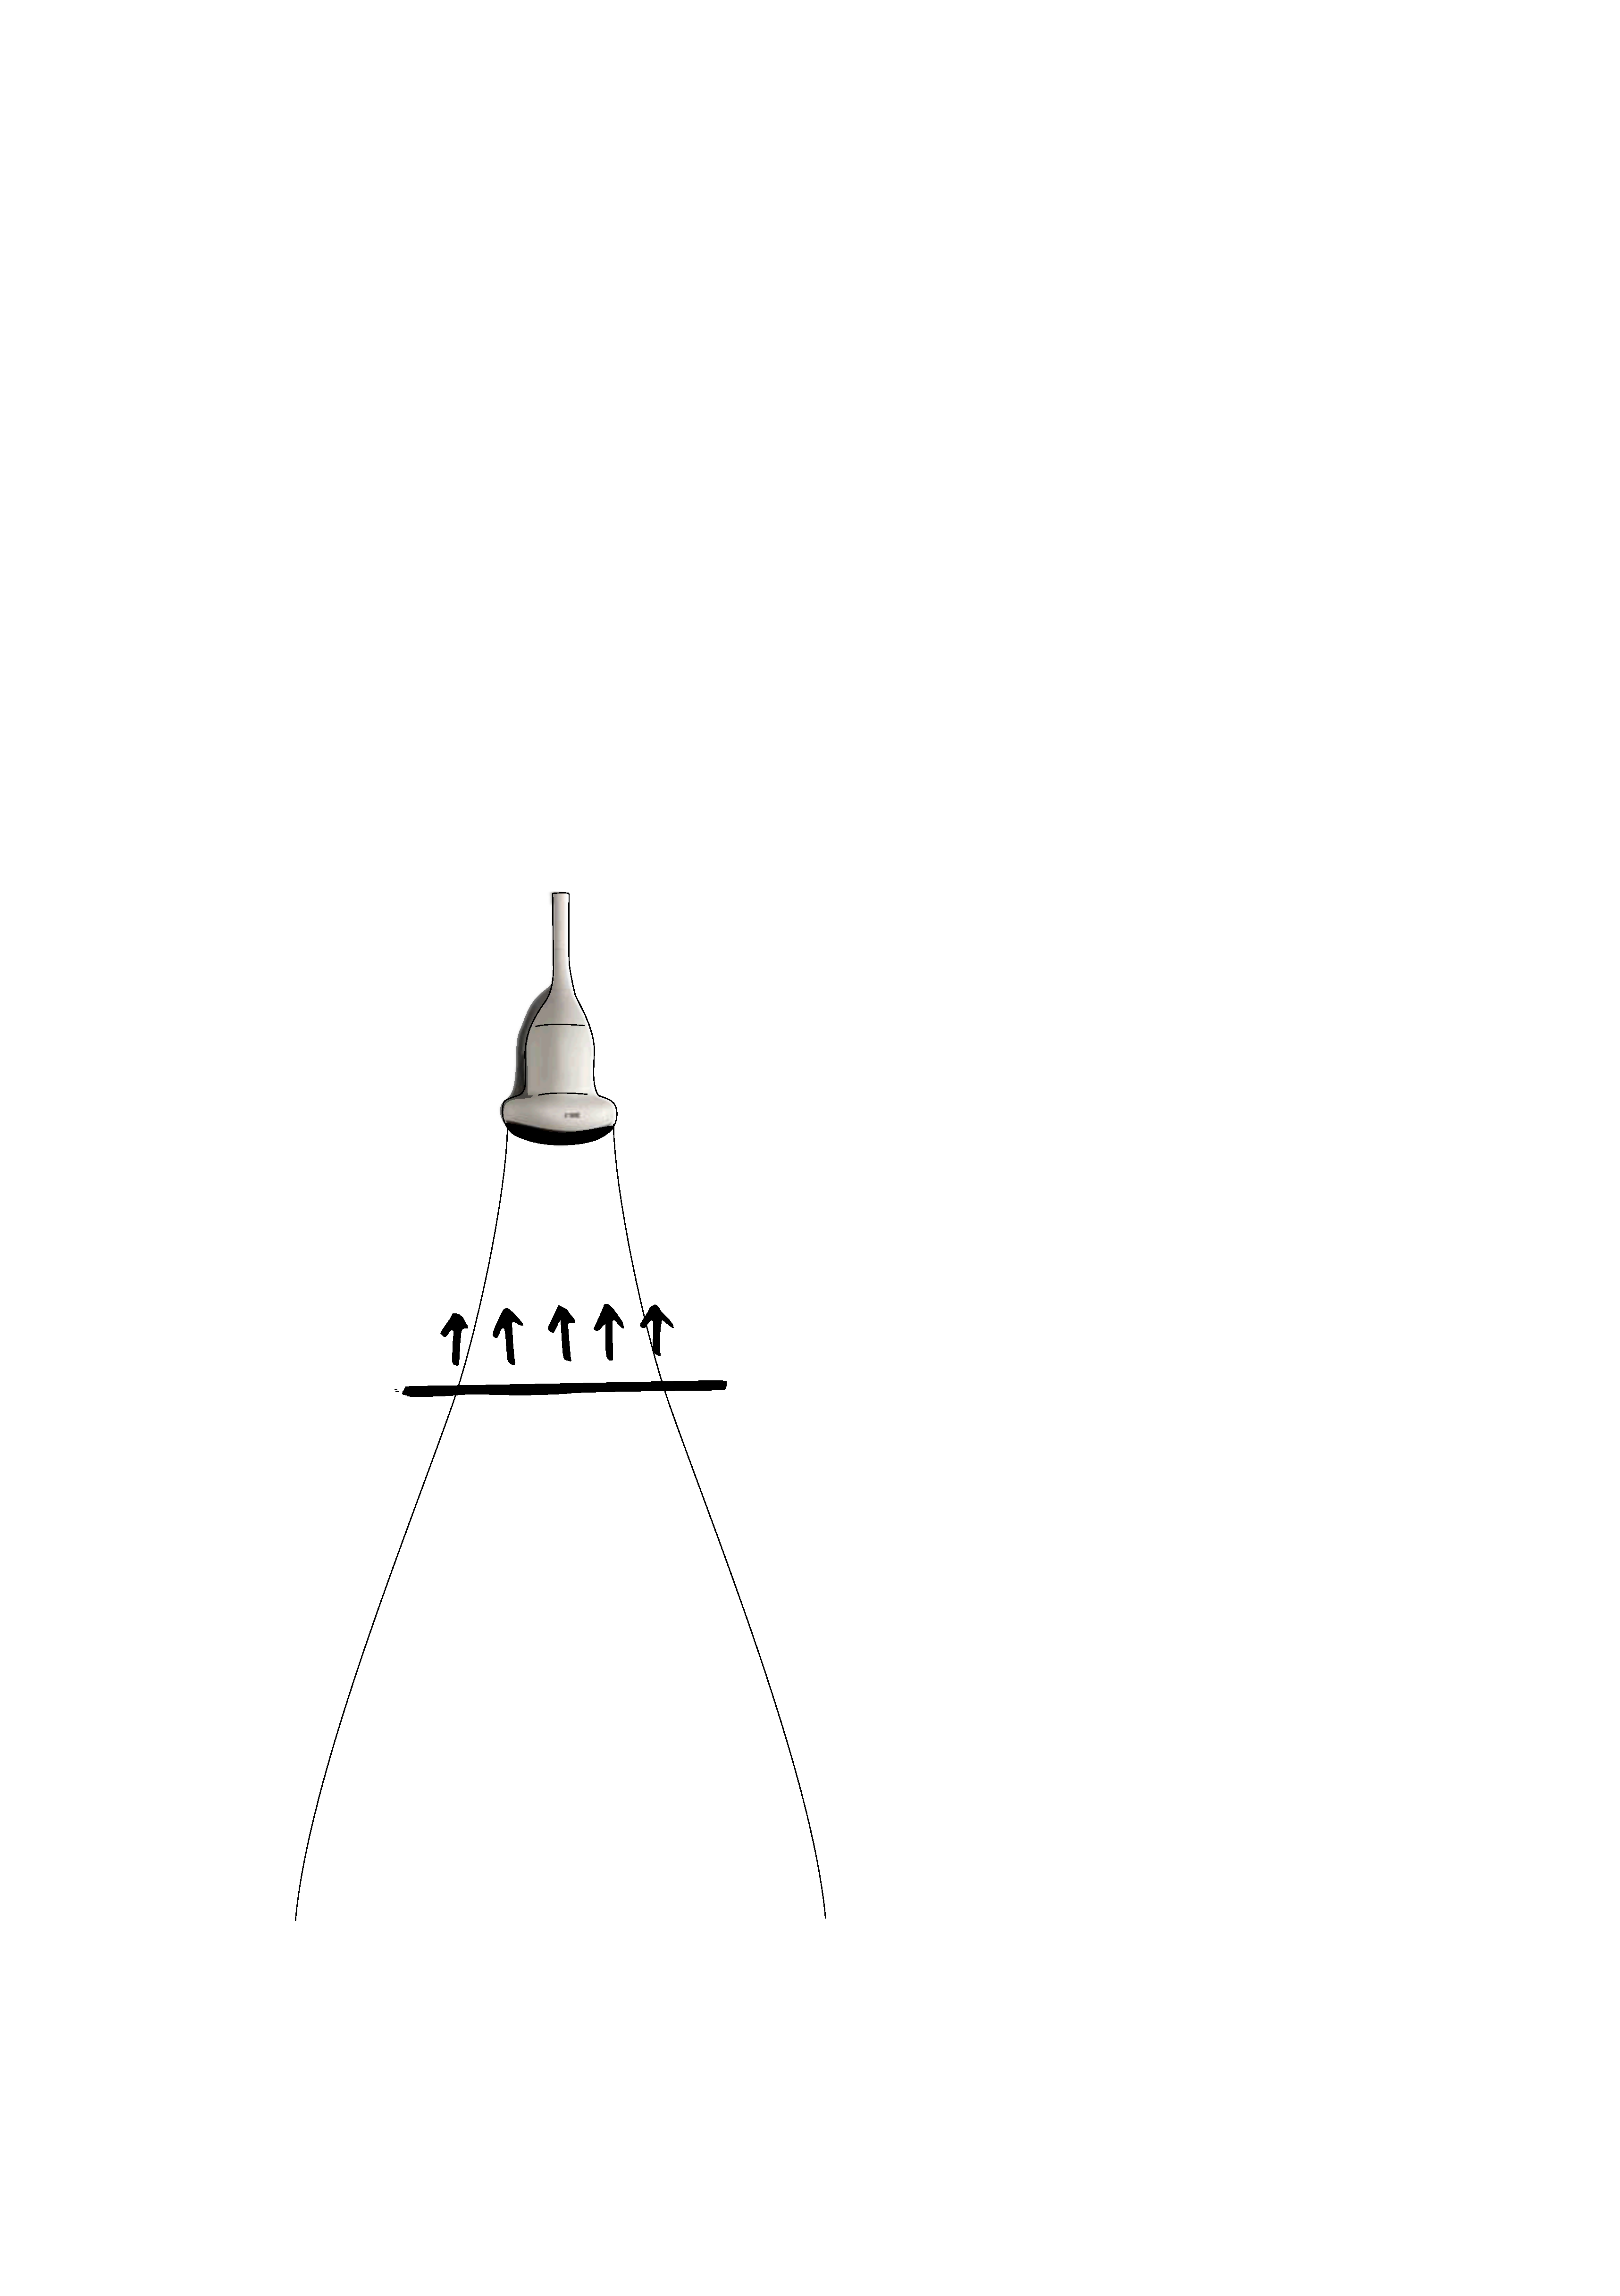
\includegraphics[trim = 300 350 800 1000, clip,width=.8\textwidth]{USscattering/master2.pdf}};
 
%    \draw[help lines,xstep=.5,ystep=.5] (0,0) grid (4,8);
%\foreach \x in {0,.5,1,...,4} { \node [anchor=north] at (\x,8) {\x}; }
%\foreach \y in {0,.5,1,...,8} { \node [anchor=east] at (0,\y) {\y}; });

\def\waveXCenter{2.1}
\def\waveIni{6.3}
\def\waveFin{1}
\def\waveAmplitud{.8}
  \draw[decorate, decoration={snake, segment length=15, amplitude=15},red] (2.03,6) -- (2.03,4.3);
  \draw[decorate, decoration={snake, segment length=15, amplitude=8},red] (2.03,4.3) -- (2.03,.9);
 
\draw 	(0.5,4.7) node[anchor=east] {$R=\frac{Z_2 - Z_1}{Z_2+Z_1}$}
			(0.5,4) node[anchor=east] {$T=\frac{2Z_2}{Z_2+Z_1}$}
			(3.2,4.7) node[anchor=west] {$Z_1$}
			(3.2,4) node[anchor=west] {$Z_2$};

\end{scriptsize}
\end{tikzpicture}
\end{column}

\begin{column}{.48\textwidth}
		\begin{figure}
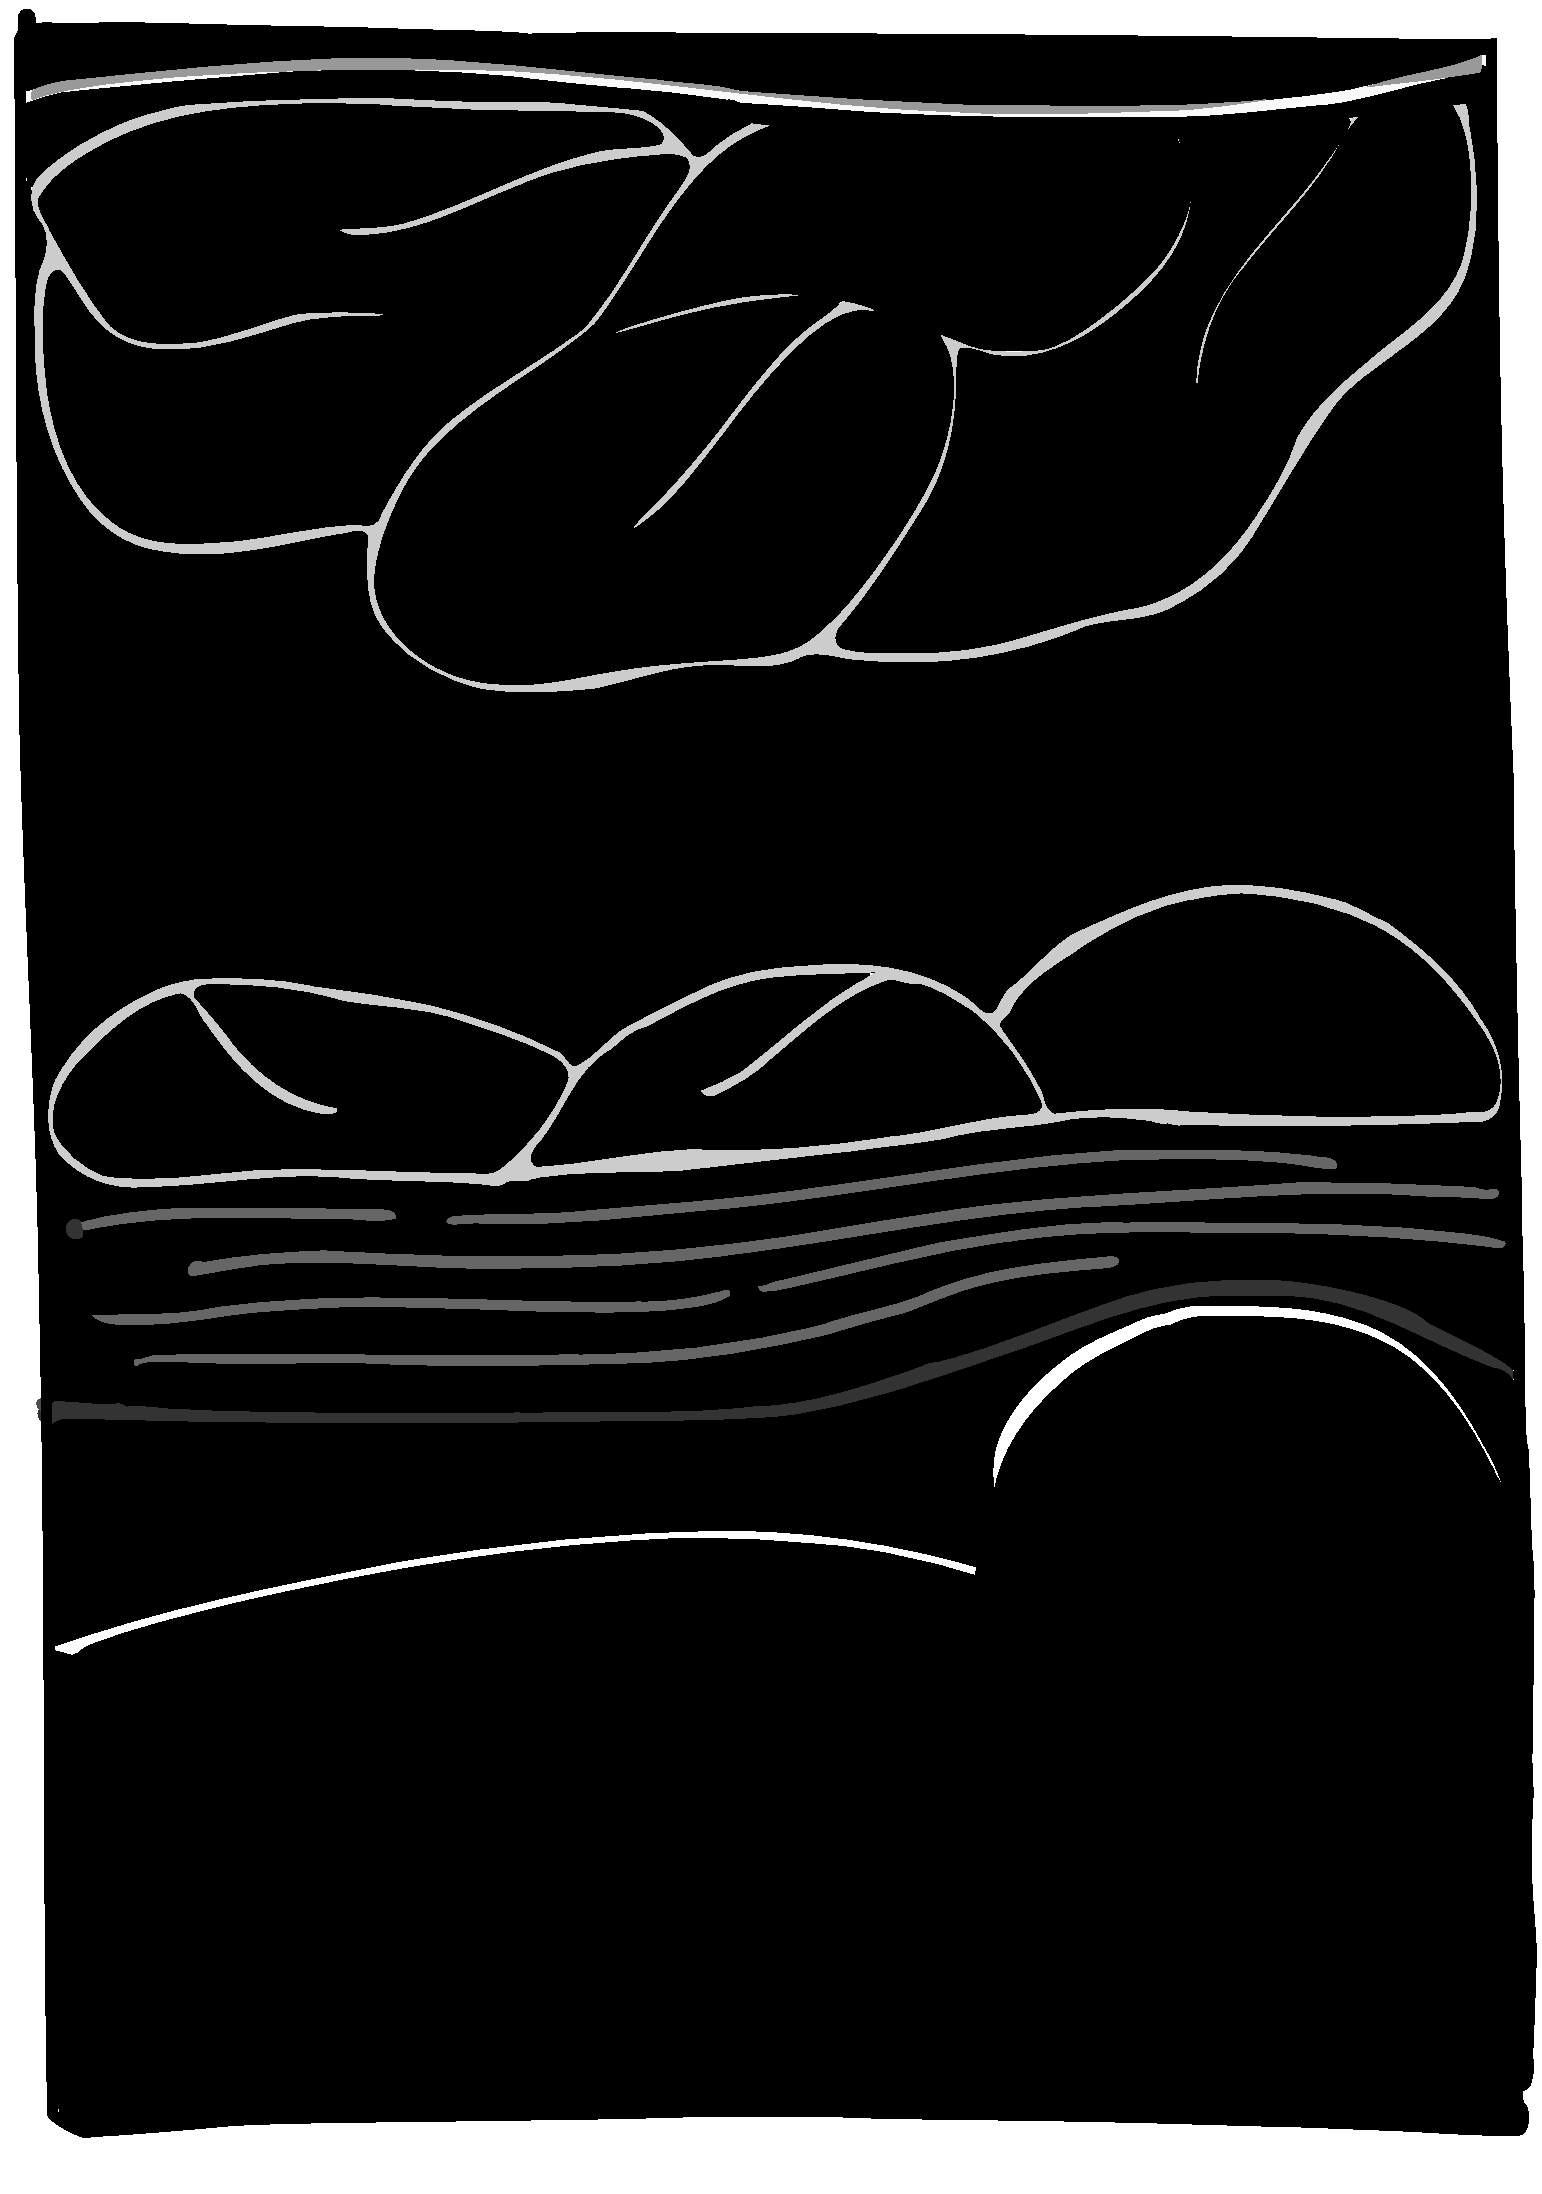
\includegraphics[width=.7\textwidth]{slice/US.pdf}
	\caption{Ideal Breast \ac{us} screening based on the depicting the reflection produced on the different tissue boundaries.}
		\end{figure}
\end{column}
\end{columns}
\end{frame}

\begin{frame}\frametitle{Breast structures and appearance under US screening}
		\begin{figure}
		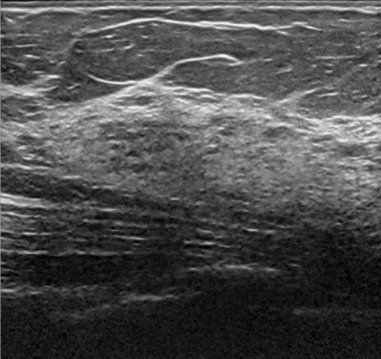
\includegraphics[height=.55\textheight]{sa1.png}~
		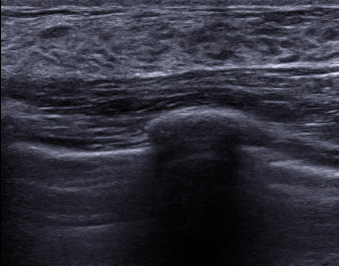
\includegraphics[height=.55\textheight]{sa2.png}
		\caption{ Ultrasound screening examples of two healthy breasts.}
		\end{figure}	
\end{frame}

\subsection{Image inspection to infer state of health}
%\subsection{Computer Aided Diagnosis (CAD)}

\begin{frame}\frametitle{State of health from image visual Inspection}
\setbeamercovered{transparent}
\begin{block}{Radiologic diagnosis error rates are similar to any other human visual inspection\footnotemark[1]}
  \begin{itemize}
    \item Quality of the images.
    \item Ability to interpret the physical properties of the images.
  \end{itemize}
\end{block}
  \begin{enumerate}
    \item <2-> Double readings.
    \item <3-> Utilization of computers to aid the radiologists during the diagnosis process\footnotemark[2]$^,$\footnotemark[3].
  \end{enumerate}
\footnotetext[1]{\fullcite{manning2005perception}}
\onslide<3>
\footnotetext[2]{\fullcite{lusted1955medical}}
%\footnotetext[3]{\fullcite{chan1990improvement}}
\footnotetext[3]{\fullcite{giger2008anniversary}}
\end{frame}


\definecolor{colorTheme}{RGB}{51,41,178}
\begin{frame}\frametitle{\tikz[baseline,inner sep=1.5pt] \node[circle,draw,thick,anchor=base] {1};~Common attributes for describing the image content}
\begin{itemize}
\vspace{-5pt}
\item BKGD Echotexture :
			adipose, fibro-glandular, heterogeneous
\item Mass shape :
	\begin{tikzpicture}[baseline=(label.north)]
	\coordinate (rect) at (.5,.5);
	\coordinate (aux) at (.5,.53);

	\begin{tiny}
		\draw (0,0) rectangle (rect);
		\draw (0.25,0) node[minimum width=1cm,anchor=north](label){Oval};
		\draw [thick,colorTheme!80!white] (0.25,0.25) ellipse ( .2 and .08);
	\end{tiny}
	
	\begin{pgfonlayer}{background}
	\fill [green!30,rounded corners=2pt] ($ (label.west) !.65! (label.south west) $) rectangle (aux -| label.east);
	\end{pgfonlayer}
	\end{tikzpicture}
		\begin{tikzpicture}[baseline=(label.north)]
	\coordinate (rect) at (.5,.5);
	\coordinate (aux) at (.5,.53);

	\begin{tiny}
		\draw (0,0) rectangle (rect);
		\draw (0.25,0) node[minimum width=1cm,anchor=north](label){Round};
%				   (.25,.25) circle[fill,radius=.18,fill=red];
		\draw [thick,colorTheme!80!white]   (.25,.25) circle[radius=.18];
	\end{tiny}
	
	\begin{pgfonlayer}{background}
	\fill [red!30,rounded corners=2pt] ($ (label.west) !.65! (label.south west) $) rectangle (aux -| label.east);
	\end{pgfonlayer}
	\end{tikzpicture} 
		\begin{tikzpicture}[baseline=(label.north)]
	\coordinate (rect) at (.5,.5);
	\coordinate (aux) at (.5,.53);

	\begin{tiny}
		\draw (0,0) rectangle (rect);
		\draw (0.25,0) node[minimum width=1cm,anchor=north](label){Irregular};
		\draw [thick,colorTheme!80!white,rounded corners=2pt]   (.05,.25) -- (.1, .1)  -- (.2,.3) -- (.3,.2)  -- (.2,.05) -- (.35,.06) -- (.45,.25) -- (.4,.46) -- (.15,.3) -- (.1,.45) -- cycle;		
	\end{tiny}
	
	\begin{pgfonlayer}{background}
	\fill [red!30,rounded corners=2pt] ($ (label.west) !.65! (label.south west) $) rectangle (aux -| label.east);
	\end{pgfonlayer}
	\end{tikzpicture}
		\begin{tikzpicture}[baseline=(label.north)]
	\coordinate (rect) at (.5,.5);
	\coordinate (aux) at (.5,.53);

	\begin{tiny}
		\draw (0,0) rectangle (rect);
		\draw (0.25,0) node[minimum width=1cm,anchor=north](label){Lobular};
		\draw [thick,colorTheme!80!white,rounded corners=2pt]   (.05,.25) -- (.18,.15) -- (.25,.25) -- (.35,.15) -- (.45,.25) -- (.35,.35) -- (.25,.25) -- (.18,.35) -- cycle;
	\end{tiny}
	
	\begin{pgfonlayer}{background}
	\fill [orange!30,rounded corners=2pt] ($ (label.west) !.65! (label.south west) $) rectangle (aux -| label.east);
	\end{pgfonlayer}
	\end{tikzpicture}
\item Mass orientation :
		\begin{tikzpicture}[baseline=(label.north)]
	\coordinate (rect) at (.5,.5);
	\coordinate (aux) at (.5,.53);

	\begin{tiny}
		\draw (0,0) rectangle (rect);
		\draw (0.25,0) node[minimum width=1cm,anchor=north](label){Parallel};
		\draw[gray] (0,.44) -- (.5,.44);
		\draw[gray] (0,.47) -- (.5,.47);
		\draw [thick,colorTheme!80!white] (0.25,0.25) ellipse ( .15 and .06);
	\end{tiny}
	
	\begin{pgfonlayer}{background}
	\fill [green!30,rounded corners=2pt] ($ (label.west) !.65! (label.south west) $) rectangle (aux -| label.east);
	\end{pgfonlayer}
	\end{tikzpicture}
		\begin{tikzpicture}[baseline=(label.north)]
	\coordinate (rect) at (.5,.5);
	\coordinate (aux) at (.5,.53);

	\begin{tiny}
		\draw (0,0) rectangle (rect);
		\draw (0.25,0) node[anchor=north](label){Non-parallel};
		\draw[gray] (0,.44) -- (.5,.44);
		\draw[gray] (0,.47) -- (.5,.47);
		\draw [thick,colorTheme!80!white] (0.25,0.25) ellipse ( .06 and .15);
	\end{tiny}
	
	\begin{pgfonlayer}{background}
	\fill [red!30,rounded corners=2pt] ($ (label.west) !.65! (label.south west) $) rectangle (aux -| label.east);
	\end{pgfonlayer}
	\end{tikzpicture}
\item Mass margin :
		\begin{tikzpicture}[baseline=(label.north)]
	\coordinate (rect) at (.5,.5);
	\coordinate (aux) at (.5,.53);

	\begin{tiny}
		%\draw (0,0) rectangle (rect);
		\node[inner sep=0pt,anchor=south west]  at (0,0) {
\includegraphics[height=.5cm]{birads/circumscribed}};
		\draw (0.25,0) node[minimum width=1cm,anchor=north](label){Circumscribed};
	\end{tiny}
	
	\begin{pgfonlayer}{background}
	\fill [green!30,rounded corners=2pt] ($ (label.west) !.65! (label.south west) $) rectangle (aux -| label.east);
	\end{pgfonlayer}
	\end{tikzpicture}
		\begin{tikzpicture}[baseline=(label.north)]
	\coordinate (rect) at (.5,.5);
	\coordinate (aux) at (.5,.53);

	\begin{tiny}
		\node[inner sep=0pt,anchor=south west]  at (0,0) {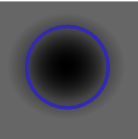
\includegraphics[height=.5cm]{birads/indistinct.png}};
		\draw (0.25,0) node[minimum width=1cm,anchor=north](label){Indistinct};
	\end{tiny}
	
	\begin{pgfonlayer}{background}
	\fill [red!30,rounded corners=2pt] ($ (label.west) !.65! (label.south west) $) rectangle (aux -| label.east);
	\end{pgfonlayer}
	\end{tikzpicture}
		\begin{tikzpicture}[baseline=(label.north)]
	\coordinate (rect) at (.5,.5);
	\coordinate (aux) at (.5,.53);

	\begin{tiny}
		\draw (0,0) rectangle (rect);
		\node[inner sep=0pt,anchor=south west]  at (.03,.12) {
\includegraphics[height=.3cm]{birads/angular}};
		\draw (0.25,0) node[minimum width=1cm,anchor=north](label){Angular};
	\end{tiny}
	
	\begin{pgfonlayer}{background}
	\fill [red!30,rounded corners=2pt] ($ (label.west) !.65! (label.south west) $) rectangle (aux -| label.east);
	\end{pgfonlayer}
	\end{tikzpicture}
		\begin{tikzpicture}[baseline=(label.north)]
	\coordinate (rect) at (.5,.5);
	\coordinate (aux) at (.5,.53);

	\begin{tiny}
			\draw (0,0) rectangle (rect);
		\node[inner sep=0pt,anchor=south west]  at (.05,.12) {
\includegraphics[height=.3cm]{birads/micro.pdf}};
		\draw (0.25,0) node[minimum width=1cm,anchor=north](label){Microlobulated};
	\end{tiny}
	
	\begin{pgfonlayer}{background}
	\fill [red!30,rounded corners=2pt] ($ (label.west) !.65! (label.south west) $) rectangle (aux -| label.east);
	\end{pgfonlayer}
	\end{tikzpicture}
		\begin{tikzpicture}[baseline=(label.north)]
	\coordinate (rect) at (.5,.5);
	\coordinate (aux) at (.5,.53);

	\begin{tiny}
		\draw (0,0) rectangle (rect);
		\node[inner sep=0pt,anchor=south west]  at (0.06,0.1) {
\includegraphics[height=.35cm]{birads/spiculated}};
		\draw (0.25,0) node[minimum width=1cm,anchor=north](label){Spiculated};
	\end{tiny}
	
	\begin{pgfonlayer}{background}
	\fill [red!30,rounded corners=2pt] ($ (label.west) !.65! (label.south west) $) rectangle (aux -| label.east);
	\end{pgfonlayer}
	\end{tikzpicture}
\item Lesion boundary :
		\begin{tikzpicture}[baseline=(label.north)]
	\coordinate (rect) at (.5,.5);
	\coordinate (aux) at (.5,.53);

	\begin{tiny}
%		\draw (0,0) rectangle (rect);
		\node[inner sep=0pt,anchor=south west]  at (0,0) {
\includegraphics[height=.5cm]{birads/Abrupt}};
		\draw (0.25,0) node[minimum width=1cm,anchor=north](label){Abrupt Interface};
	\end{tiny}
	
	\begin{pgfonlayer}{background}
	\fill [green!30,rounded corners=2pt] ($ (label.west) !.65! (label.south west) $) rectangle (aux -| label.east);
	\end{pgfonlayer}
	\end{tikzpicture}
		\begin{tikzpicture}[baseline=(label.north)]
	\coordinate (rect) at (.5,.5);
	\coordinate (aux) at (.5,.53);

	\begin{tiny}
%		\draw (0,0) rectangle (rect);
		\node[inner sep=0pt,anchor=south west]  at (0,0) {
\includegraphics[height=.5cm]{birads/halo}};
		\draw (0.25,0) node[minimum width=1cm,anchor=north](label){Echogenic halo};
	\end{tiny}
	
	\begin{pgfonlayer}{background}
	\fill [red!30,rounded corners=2pt] ($ (label.west) !.65! (label.south west) $) rectangle (aux -| label.east);
	\end{pgfonlayer}
	\end{tikzpicture}
\item Echo pattern :
		\begin{tikzpicture}[baseline=(label.north)]
	\coordinate (rect) at (.5,.5);
	\coordinate (aux) at (.5,.53);

	\begin{tiny}
		\node[inner sep=0pt,anchor=south west]  at (0,0) {
\includegraphics[height=.5cm]{birads/anechoic}};
		\draw (0.25,0) node[minimum width=1cm,anchor=north](label){Anechoic};
	\end{tiny}
	
	\begin{pgfonlayer}{background}
	\fill [green!30,rounded corners=2pt] ($ (label.west) !.65! (label.south west) $) rectangle (aux -| label.east);
	\end{pgfonlayer}
	\end{tikzpicture}
		\begin{tikzpicture}[baseline=(label.north)]
	\coordinate (rect) at (.5,.5);
	\coordinate (aux) at (.5,.53);

	\begin{tiny}
		\node[inner sep=0pt,anchor=south west]  at (0,0) {
\includegraphics[height=.5cm]{birads/hyperechoic}};
		\draw (0.25,0) node[minimum width=1cm,anchor=north](label){Hyperechoic};
	\end{tiny}
	
	\begin{pgfonlayer}{background}
	\fill [green!30,rounded corners=2pt] ($ (label.west) !.65! (label.south west) $) rectangle (aux -| label.east);
	\end{pgfonlayer}
	\end{tikzpicture}
		\begin{tikzpicture}[baseline=(label.north)]
	\coordinate (rect) at (.5,.5);
	\coordinate (aux) at (.5,.53);

	\begin{tiny}
\node[inner sep=0pt,anchor=south west]  at (0,0) {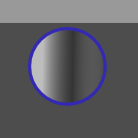
\includegraphics[height=.5cm]{birads/complex.png}};
		\draw (0.25,0) node[minimum width=1cm,anchor=north](label){Complex};
	\end{tiny}
	
	\begin{pgfonlayer}{background}
	\fill [red!30,rounded corners=2pt] ($ (label.west) !.65! (label.south west) $) rectangle (aux -| label.east);
	\end{pgfonlayer}
	\end{tikzpicture}
		\begin{tikzpicture}[baseline=(label.north)]
	\coordinate (rect) at (.5,.5);
	\coordinate (aux) at (.5,.53);

	\begin{tiny}
%		\draw (0,0) rectangle (rect);
		\node[inner sep=0pt,anchor=south west]  at (0,0) {
\includegraphics[height=.5cm]{birads/isoechoic}};
		\draw (0.25,0) node[minimum width=1cm,anchor=north](label){Isoechoic};
	\end{tiny}
	
	\begin{pgfonlayer}{background}
	\fill [orange!30,rounded corners=2pt] ($ (label.west) !.65! (label.south west) $) rectangle (aux -| label.east);
	\end{pgfonlayer}
	\end{tikzpicture}
		\begin{tikzpicture}[baseline=(label.north)]
	\coordinate (rect) at (.5,.5);
	\coordinate (aux) at (.5,.53);

	\begin{tiny}
		\node[inner sep=0pt,anchor=south west]  at (0,0) {
\includegraphics[height=.5cm]{birads/hypoechoic}};
		\draw (0.25,0) node[minimum width=1cm,anchor=north](label){Hypoechoic};
	\end{tiny}
	
	\begin{pgfonlayer}{background}
	\fill [orange!30,rounded corners=2pt] ($ (label.west) !.65! (label.south west) $) rectangle (aux -| label.east);
	\end{pgfonlayer}
	\end{tikzpicture}
\item Posterior acoustic pattern : 
		\begin{tikzpicture}[baseline=(label.north)]
	\coordinate (rect) at (.5,.5);
	\coordinate (aux) at (.5,.53);

	\begin{tiny}
\node[inner sep=0pt,anchor=south west]  at (0,0) {
\includegraphics[height=.5cm]{birads/shadow}};
		\draw (0.25,0) node[minimum width=1cm,anchor=north](label){Shadowing};
	\end{tiny}
	
	\begin{pgfonlayer}{background}
	\fill [red!30,rounded corners=2pt] ($ (label.west) !.65! (label.south west) $) rectangle (aux -| label.east);
	\end{pgfonlayer}
	\end{tikzpicture}
		\begin{tikzpicture}[baseline=(label.north)]
	\coordinate (rect) at (.5,.5);
	\coordinate (aux) at (.5,.53);

	\begin{tiny}
\node[inner sep=0pt,anchor=south west]  at (0,0) {
\includegraphics[height=.5cm]{birads/combined}};
		\draw (0.25,0) node[minimum width=1cm,anchor=north](label){Combined};
	\end{tiny}
	
	\begin{pgfonlayer}{background}
	\fill [red!30,rounded corners=2pt] ($ (label.west) !.65! (label.south west) $) rectangle (aux -| label.east);
	\end{pgfonlayer}
	\end{tikzpicture}
		\begin{tikzpicture}[baseline=(label.north)]
	\coordinate (rect) at (.5,.5);
	\coordinate (aux) at (.5,.53);

	\begin{tiny}
\node[inner sep=0pt,anchor=south west]  at (0,0) {
\includegraphics[height=.5cm]{birads/enhance}};
		\draw (0.25,0) node[minimum width=1cm,anchor=north](label){Enhancement};
	\end{tiny}
	
	\begin{pgfonlayer}{background}
	\fill [orange!30,rounded corners=2pt] ($ (label.west) !.65! (label.south west) $) rectangle (aux -| label.east);
	\end{pgfonlayer}
	\end{tikzpicture}
		\begin{tikzpicture}[baseline=(label.north)]
	\coordinate (rect) at (.5,.5);
	\coordinate (aux) at (.5,.53);

	\begin{tiny}
\node[inner sep=0pt,anchor=south west]  at (0,0) {
\includegraphics[height=.5cm]{birads/hypoechoic}};
		\draw (0.25,0) node[minimum width=1cm,anchor=north](label){No pattern};
	\end{tiny}
	
	\begin{pgfonlayer}{background}
	\fill [orange!30,rounded corners=2pt] ($ (label.west) !.65! (label.south west) $) rectangle (aux -| label.east);
	\end{pgfonlayer}
	\end{tikzpicture}
\end{itemize}

\footnotetext{~\tikz[baseline=(x),inner sep=1.5pt] {\coordinate (x) at (0,-3pt); \node[fill=green!30,rounded corners=2pt,anchor=base,minimum size=10pt] {};} benign, \tikz[baseline=(x),inner sep=1.5pt] {\coordinate (x) at (0,-3pt); \node[fill=red!30,rounded corners=2pt,anchor=base,minimum size=10pt] {};} malignant and \tikz[baseline=(x),inner sep=1.5pt] {\coordinate (x) at (0,-3pt); \node[fill=orange!30,rounded corners=2pt,anchor=base,minimum size=10pt] {};} undetermined founds obtained from a compound of medical works\footnotemark[1].}
\footnotetext[1]{\fullcite{raza2010us}}
\end{frame}


\begin{frame}\frametitle{\tikz[baseline,inner sep=1.5pt] \node[circle,draw,thick,anchor=base] {2};~\acf{cad}}
\vspace{-10pt}
\begin{small}
\begin{block}{\acf{cade}}
{\footnotesize
implies that radiologists use computer outputs of the locations of suspect regions, leaving the characterization, diagnosis, and patient management to be done manually.}
\end{block}
\begin{block}{\acf{cadx}}
{\footnotesize
extends the computer analyses to yield output on the characterization of a region or 
lesion, initially located by either a human or a \ac{cade} system.
}
\end{block}
\vspace{-8pt}
\begin{itemize}
\item 
Most of the descriptors used to describe breast lesions in US data for diagnosis purposes are based on lexicon tools\footnotemark[1]$^,$\footnotemark[2].
\end{itemize}
\end{small}
\footnotetext[1]{\fullcite{Cheng:2009p10580}}
\footnotetext[2]{\fullcite{jalalian2012computer}}
\end{frame}

\begin{frame}\frametitle{Take away}
\item BKGD Echotexture :
			adipose, fibro-glandular, heterogeneous
\item Mass shape :
	\begin{tikzpicture}[baseline=(label.north)]
	\coordinate (rect) at (.5,.5);
	\coordinate (aux) at (.5,.53);

	\begin{tiny}
		\draw (0,0) rectangle (rect);
		\draw (0.25,0) node[minimum width=1cm,anchor=north](label){Oval};
		\draw [thick,colorTheme!80!white] (0.25,0.25) ellipse ( .2 and .08);
	\end{tiny}
	
	\begin{pgfonlayer}{background}
	\fill [green!30,rounded corners=2pt] ($ (label.west) !.65! (label.south west) $) rectangle (aux -| label.east);
	\end{pgfonlayer}
	\end{tikzpicture}
		\begin{tikzpicture}[baseline=(label.north)]
	\coordinate (rect) at (.5,.5);
	\coordinate (aux) at (.5,.53);

	\begin{tiny}
		\draw (0,0) rectangle (rect);
		\draw (0.25,0) node[minimum width=1cm,anchor=north](label){Round};
%				   (.25,.25) circle[fill,radius=.18,fill=red];
		\draw [thick,colorTheme!80!white]   (.25,.25) circle[radius=.18];
	\end{tiny}
	
	\begin{pgfonlayer}{background}
	\fill [red!30,rounded corners=2pt] ($ (label.west) !.65! (label.south west) $) rectangle (aux -| label.east);
	\end{pgfonlayer}
	\end{tikzpicture} 
		\begin{tikzpicture}[baseline=(label.north)]
	\coordinate (rect) at (.5,.5);
	\coordinate (aux) at (.5,.53);

	\begin{tiny}
		\draw (0,0) rectangle (rect);
		\draw (0.25,0) node[minimum width=1cm,anchor=north](label){Irregular};
		\draw [thick,colorTheme!80!white,rounded corners=2pt]   (.05,.25) -- (.1, .1)  -- (.2,.3) -- (.3,.2)  -- (.2,.05) -- (.35,.06) -- (.45,.25) -- (.4,.46) -- (.15,.3) -- (.1,.45) -- cycle;		
	\end{tiny}
	
	\begin{pgfonlayer}{background}
	\fill [red!30,rounded corners=2pt] ($ (label.west) !.65! (label.south west) $) rectangle (aux -| label.east);
	\end{pgfonlayer}
	\end{tikzpicture}
		\begin{tikzpicture}[baseline=(label.north)]
	\coordinate (rect) at (.5,.5);
	\coordinate (aux) at (.5,.53);

	\begin{tiny}
		\draw (0,0) rectangle (rect);
		\draw (0.25,0) node[minimum width=1cm,anchor=north](label){Lobular};
		\draw [thick,colorTheme!80!white,rounded corners=2pt]   (.05,.25) -- (.18,.15) -- (.25,.25) -- (.35,.15) -- (.45,.25) -- (.35,.35) -- (.25,.25) -- (.18,.35) -- cycle;
	\end{tiny}
	
	\begin{pgfonlayer}{background}
	\fill [orange!30,rounded corners=2pt] ($ (label.west) !.65! (label.south west) $) rectangle (aux -| label.east);
	\end{pgfonlayer}
	\end{tikzpicture}
\item Mass orientation :
		\begin{tikzpicture}[baseline=(label.north)]
	\coordinate (rect) at (.5,.5);
	\coordinate (aux) at (.5,.53);

	\begin{tiny}
		\draw (0,0) rectangle (rect);
		\draw (0.25,0) node[minimum width=1cm,anchor=north](label){Parallel};
		\draw[gray] (0,.44) -- (.5,.44);
		\draw[gray] (0,.47) -- (.5,.47);
		\draw [thick,colorTheme!80!white] (0.25,0.25) ellipse ( .15 and .06);
	\end{tiny}
	
	\begin{pgfonlayer}{background}
	\fill [green!30,rounded corners=2pt] ($ (label.west) !.65! (label.south west) $) rectangle (aux -| label.east);
	\end{pgfonlayer}
	\end{tikzpicture}
		\begin{tikzpicture}[baseline=(label.north)]
	\coordinate (rect) at (.5,.5);
	\coordinate (aux) at (.5,.53);

	\begin{tiny}
		\draw (0,0) rectangle (rect);
		\draw (0.25,0) node[anchor=north](label){Non-parallel};
		\draw[gray] (0,.44) -- (.5,.44);
		\draw[gray] (0,.47) -- (.5,.47);
		\draw [thick,colorTheme!80!white] (0.25,0.25) ellipse ( .06 and .15);
	\end{tiny}
	
	\begin{pgfonlayer}{background}
	\fill [red!30,rounded corners=2pt] ($ (label.west) !.65! (label.south west) $) rectangle (aux -| label.east);
	\end{pgfonlayer}
	\end{tikzpicture}
\item Mass margin :
		\begin{tikzpicture}[baseline=(label.north)]
	\coordinate (rect) at (.5,.5);
	\coordinate (aux) at (.5,.53);

	\begin{tiny}
		%\draw (0,0) rectangle (rect);
		\node[inner sep=0pt,anchor=south west]  at (0,0) {
\includegraphics[height=.5cm]{birads/circumscribed}};
		\draw (0.25,0) node[minimum width=1cm,anchor=north](label){Circumscribed};
	\end{tiny}
	
	\begin{pgfonlayer}{background}
	\fill [green!30,rounded corners=2pt] ($ (label.west) !.65! (label.south west) $) rectangle (aux -| label.east);
	\end{pgfonlayer}
	\end{tikzpicture}
		\begin{tikzpicture}[baseline=(label.north)]
	\coordinate (rect) at (.5,.5);
	\coordinate (aux) at (.5,.53);

	\begin{tiny}
		\node[inner sep=0pt,anchor=south west]  at (0,0) {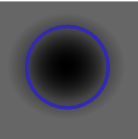
\includegraphics[height=.5cm]{birads/indistinct.png}};
		\draw (0.25,0) node[minimum width=1cm,anchor=north](label){Indistinct};
	\end{tiny}
	
	\begin{pgfonlayer}{background}
	\fill [red!30,rounded corners=2pt] ($ (label.west) !.65! (label.south west) $) rectangle (aux -| label.east);
	\end{pgfonlayer}
	\end{tikzpicture}
		\begin{tikzpicture}[baseline=(label.north)]
	\coordinate (rect) at (.5,.5);
	\coordinate (aux) at (.5,.53);

	\begin{tiny}
		\draw (0,0) rectangle (rect);
		\node[inner sep=0pt,anchor=south west]  at (.03,.12) {
\includegraphics[height=.3cm]{birads/angular}};
		\draw (0.25,0) node[minimum width=1cm,anchor=north](label){Angular};
	\end{tiny}
	
	\begin{pgfonlayer}{background}
	\fill [red!30,rounded corners=2pt] ($ (label.west) !.65! (label.south west) $) rectangle (aux -| label.east);
	\end{pgfonlayer}
	\end{tikzpicture}
		\begin{tikzpicture}[baseline=(label.north)]
	\coordinate (rect) at (.5,.5);
	\coordinate (aux) at (.5,.53);

	\begin{tiny}
			\draw (0,0) rectangle (rect);
		\node[inner sep=0pt,anchor=south west]  at (.05,.12) {
\includegraphics[height=.3cm]{birads/micro.pdf}};
		\draw (0.25,0) node[minimum width=1cm,anchor=north](label){Microlobulated};
	\end{tiny}
	
	\begin{pgfonlayer}{background}
	\fill [red!30,rounded corners=2pt] ($ (label.west) !.65! (label.south west) $) rectangle (aux -| label.east);
	\end{pgfonlayer}
	\end{tikzpicture}
		\begin{tikzpicture}[baseline=(label.north)]
	\coordinate (rect) at (.5,.5);
	\coordinate (aux) at (.5,.53);

	\begin{tiny}
		\draw (0,0) rectangle (rect);
		\node[inner sep=0pt,anchor=south west]  at (0.06,0.1) {
\includegraphics[height=.35cm]{birads/spiculated}};
		\draw (0.25,0) node[minimum width=1cm,anchor=north](label){Spiculated};
	\end{tiny}
	
	\begin{pgfonlayer}{background}
	\fill [red!30,rounded corners=2pt] ($ (label.west) !.65! (label.south west) $) rectangle (aux -| label.east);
	\end{pgfonlayer}
	\end{tikzpicture}
\item Lesion boundary :
		\begin{tikzpicture}[baseline=(label.north)]
	\coordinate (rect) at (.5,.5);
	\coordinate (aux) at (.5,.53);

	\begin{tiny}
%		\draw (0,0) rectangle (rect);
		\node[inner sep=0pt,anchor=south west]  at (0,0) {
\includegraphics[height=.5cm]{birads/Abrupt}};
		\draw (0.25,0) node[minimum width=1cm,anchor=north](label){Abrupt Interface};
	\end{tiny}
	
	\begin{pgfonlayer}{background}
	\fill [green!30,rounded corners=2pt] ($ (label.west) !.65! (label.south west) $) rectangle (aux -| label.east);
	\end{pgfonlayer}
	\end{tikzpicture}
		\begin{tikzpicture}[baseline=(label.north)]
	\coordinate (rect) at (.5,.5);
	\coordinate (aux) at (.5,.53);

	\begin{tiny}
%		\draw (0,0) rectangle (rect);
		\node[inner sep=0pt,anchor=south west]  at (0,0) {
\includegraphics[height=.5cm]{birads/halo}};
		\draw (0.25,0) node[minimum width=1cm,anchor=north](label){Echogenic halo};
	\end{tiny}
	
	\begin{pgfonlayer}{background}
	\fill [red!30,rounded corners=2pt] ($ (label.west) !.65! (label.south west) $) rectangle (aux -| label.east);
	\end{pgfonlayer}
	\end{tikzpicture}
\item Echo pattern :
		\begin{tikzpicture}[baseline=(label.north)]
	\coordinate (rect) at (.5,.5);
	\coordinate (aux) at (.5,.53);

	\begin{tiny}
		\node[inner sep=0pt,anchor=south west]  at (0,0) {
\includegraphics[height=.5cm]{birads/anechoic}};
		\draw (0.25,0) node[minimum width=1cm,anchor=north](label){Anechoic};
	\end{tiny}
	
	\begin{pgfonlayer}{background}
	\fill [green!30,rounded corners=2pt] ($ (label.west) !.65! (label.south west) $) rectangle (aux -| label.east);
	\end{pgfonlayer}
	\end{tikzpicture}
		\begin{tikzpicture}[baseline=(label.north)]
	\coordinate (rect) at (.5,.5);
	\coordinate (aux) at (.5,.53);

	\begin{tiny}
		\node[inner sep=0pt,anchor=south west]  at (0,0) {
\includegraphics[height=.5cm]{birads/hyperechoic}};
		\draw (0.25,0) node[minimum width=1cm,anchor=north](label){Hyperechoic};
	\end{tiny}
	
	\begin{pgfonlayer}{background}
	\fill [green!30,rounded corners=2pt] ($ (label.west) !.65! (label.south west) $) rectangle (aux -| label.east);
	\end{pgfonlayer}
	\end{tikzpicture}
		\begin{tikzpicture}[baseline=(label.north)]
	\coordinate (rect) at (.5,.5);
	\coordinate (aux) at (.5,.53);

	\begin{tiny}
\node[inner sep=0pt,anchor=south west]  at (0,0) {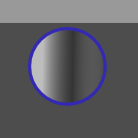
\includegraphics[height=.5cm]{birads/complex.png}};
		\draw (0.25,0) node[minimum width=1cm,anchor=north](label){Complex};
	\end{tiny}
	
	\begin{pgfonlayer}{background}
	\fill [red!30,rounded corners=2pt] ($ (label.west) !.65! (label.south west) $) rectangle (aux -| label.east);
	\end{pgfonlayer}
	\end{tikzpicture}
		\begin{tikzpicture}[baseline=(label.north)]
	\coordinate (rect) at (.5,.5);
	\coordinate (aux) at (.5,.53);

	\begin{tiny}
%		\draw (0,0) rectangle (rect);
		\node[inner sep=0pt,anchor=south west]  at (0,0) {
\includegraphics[height=.5cm]{birads/isoechoic}};
		\draw (0.25,0) node[minimum width=1cm,anchor=north](label){Isoechoic};
	\end{tiny}
	
	\begin{pgfonlayer}{background}
	\fill [orange!30,rounded corners=2pt] ($ (label.west) !.65! (label.south west) $) rectangle (aux -| label.east);
	\end{pgfonlayer}
	\end{tikzpicture}
		\begin{tikzpicture}[baseline=(label.north)]
	\coordinate (rect) at (.5,.5);
	\coordinate (aux) at (.5,.53);

	\begin{tiny}
		\node[inner sep=0pt,anchor=south west]  at (0,0) {
\includegraphics[height=.5cm]{birads/hypoechoic}};
		\draw (0.25,0) node[minimum width=1cm,anchor=north](label){Hypoechoic};
	\end{tiny}
	
	\begin{pgfonlayer}{background}
	\fill [orange!30,rounded corners=2pt] ($ (label.west) !.65! (label.south west) $) rectangle (aux -| label.east);
	\end{pgfonlayer}
	\end{tikzpicture}
\item Posterior acoustic pattern : 
		\begin{tikzpicture}[baseline=(label.north)]
	\coordinate (rect) at (.5,.5);
	\coordinate (aux) at (.5,.53);

	\begin{tiny}
\node[inner sep=0pt,anchor=south west]  at (0,0) {\includegraphics[height=.5cm]{birads/shadow}};
		\draw (0.25,0) node[minimum width=1cm,anchor=north](label){Shadowing};
	\end{tiny}
	
	\begin{pgfonlayer}{background}
	\fill [red!30,rounded corners=2pt] ($ (label.west) !.65! (label.south west) $) rectangle (aux -| label.east);
	\end{pgfonlayer}
	\end{tikzpicture}
		\begin{tikzpicture}[baseline=(label.north)]
	\coordinate (rect) at (.5,.5);
	\coordinate (aux) at (.5,.53);

	\begin{tiny}
\node[inner sep=0pt,anchor=south west]  at (0,0) {\includegraphics[height=.5cm]{birads/combined}};
		\draw (0.25,0) node[minimum width=1cm,anchor=north](label){Combined};
	\end{tiny}
	
	\begin{pgfonlayer}{background}
	\fill [red!30,rounded corners=2pt] ($ (label.west) !.65! (label.south west) $) rectangle (aux -| label.east);
	\end{pgfonlayer}
	\end{tikzpicture}
		\begin{tikzpicture}[baseline=(label.north)]
	\coordinate (rect) at (.5,.5);
	\coordinate (aux) at (.5,.53);

	\begin{tiny}
\node[inner sep=0pt,anchor=south west]  at (0,0) {\includegraphics[height=.5cm]{birads/enhance}};
		\draw (0.25,0) node[minimum width=1cm,anchor=north](label){Enhancement};
	\end{tiny}
	
	\begin{pgfonlayer}{background}
	\fill [orange!30,rounded corners=2pt] ($ (label.west) !.65! (label.south west) $) rectangle (aux -| label.east);
	\end{pgfonlayer}
	\end{tikzpicture}
		\begin{tikzpicture}[baseline=(label.north)]
	\coordinate (rect) at (.5,.5);
	\coordinate (aux) at (.5,.53);

	\begin{tiny}
\node[inner sep=0pt,anchor=south west]  at (0,0) {\includegraphics[height=.5cm]{birads/hypoechoic}};
		\draw (0.25,0) node[minimum width=1cm,anchor=north](label){No pattern};
	\end{tiny}
	
	\begin{pgfonlayer}{background}
	\fill [orange!30,rounded corners=2pt] ($ (label.west) !.65! (label.south west) $) rectangle (aux -| label.east);
	\end{pgfonlayer}
	\end{tikzpicture}
\end{itemize}

\end{frame}

\begin{frame}\frametitle{Wrapping up}
\begin{small}
\begin{itemize}
\item Breast cancer has huge incidence in the population\footnotemark[1].
\item \ac{us} screening is recognized as a useful adjunct image modality\footnotemark[2].
\item Lexicon tools set the standard for breast \ac{us} image reading\footnotemark[3].
\item \ac{cad} systems are proven to help radiologists' to perform more accurate diagnose\footnotemark[4].
\item Reliable \ac{cadx} features are subject to accurate delineation of the lesions\footnotemark[5].
\end{itemize}
\end{small}
\footnotetext[1]{\fullcite{cancerStatistics2011}}
\footnotetext[2]{\vspace{-1pt}\fullcite{smith2003american}}
\footnotetext[3]{\vspace{-1pt}\fullcite{biradsus}}
\footnotetext[4]{\fullcite{giger2008anniversary}}
\footnotetext[5]{\fullcite{jalalian2012computer}}
\end{frame}

\begin{frame}\frametitle{Thesis objective}
\vspace{-5pt}
\begin{block}{Need of accurate delineation of the lesions}
{Development of automatic procedures for segmenting breast lesions in US data.}
\end{block}
\begin{figure}
\includegraphics[trim=0 6 0 0,clip,height=.5\textheight]{a110105_094.png}~
\includegraphics[trim=6 0 0 0,clip,height=.5\textheight]{segment.png}
\caption{Breast \acf{dic} lesion example. Left: original image. Right: several manual delineations generated by 7 different trained experts.}
\end{figure}
\end{frame}


\section{Optimization Based Segmentation}
\begin{frame}
  \begin{beamercolorbox}[wd=\paperwidth,ht=\paperheight]{frametitle}
    \begin{tikzpicture}
      \fill[nicewhite, opacity=1] (0, 0) rectangle(1, 1);
      \node [anchor=center] (cloud) at 
        (0.5\paperwidth, 0.5\paperheight)
        {\includegraphics[width=.95\paperwidth]{method.png}};
    \end{tikzpicture}
  \end{beamercolorbox}
\end{frame}
\graphicspath{{chapters/method/figures/}}
\subsection{dummy_subsection_a}

\begin{frame}\frametitle{Optimization}
\framesubtitle{For image segmentation}
\setbeamercovered{transparent}
\onslide<2|handout:0>

\begin{equation*}
\hat{\omega} = \arg \min_{\substack{\omega}} \,U(\omega)
\end{equation*} 

\vspace{-40pt}
\begin{columns}
\begin{column}{.6\textwidth}
\begin{figure}
\center
	\begin{tikzpicture}[scale=1.63]%[y=0.080pt, x=0.08pt,yscale=1, inner sep=0pt, outer sep=0pt]
	\fill 		(1.2,1.835) circle[fill=red,radius=1.2pt];
	\draw[dashed] (.1,1.835) -- (1.2,1.835) (1.2,0) -- (1.2,1.835);
	\node[anchor=south west,inner sep=0] at (0,0) {\includegraphics[height=5cm]{SApathLong}};

	\begin{tiny}
		\draw
			   (0,1.835)node[anchor=east]{$U(\omega)$}
			   (1.2,0) node[anchor=north] {$\omega$}
		;
	\end{tiny}	
						
	\begin{scriptsize}
		\draw (0,3) node[anchor=east] {$U(\cdot)$}
			   (3.8,0.2) node[anchor=north west] {$\mathcal{W}$}
	   	;
	\end{scriptsize}
	\end{tikzpicture}
	\end{figure}
\end{column}
\begin{column}{.4\textwidth}
  \begin{block}{Considerations}
    \begin{itemize}
      \item Search Space $\mathcal{W}$
      \item Cost Function $U(\cdot)$
        \item Minimization Strategy
    \end{itemize}
  \end{block}
\end{column}
\end{columns}
\end{frame}

\begin{frame}\frametitle{Image Segmentation by Optimization}
\framesubtitle{The Metric Labeling Problem}
\setbeamercovered{transparent}

\begin{equation*}
U(\omega) = \sum_{s\in S} D_s(\omega_s) + \sum_{s}\sum_{r \in \mathcal{N}_{s}} V_{s,r}(\omega_s,\omega_r)
\end{equation*} 

\vspace{-40pt}
\begin{columns}
\begin{column}{.6\textwidth}
\begin{figure}
\center
	\begin{tikzpicture}[scale=1.63]%[y=0.080pt, x=0.08pt,yscale=1, inner sep=0pt, outer sep=0pt]
	\fill 		(1.2,1.835) circle[fill=red,radius=1.2pt];
	\draw[dashed] (.1,1.835) -- (1.2,1.835) (1.2,0) -- (1.2,1.835);
	\node[anchor=south west,inner sep=0] at (0,0) {\includegraphics[height=5cm]{SApathLong}};

	% \def\xYellow{.4}
	% \def\xBlue{3.5}
	% \def\xTrueSeg{1.95}
	% \def\xDataSeg{2.79}
	% \def\yIcon{-.05}
 	% \node[anchor=north,inner sep=0] at (\xYellow,\yIcon) {\includegraphics[height=.8cm]{yellow}};
  % \node[anchor=north,inner sep=0] at (\xTrueSeg,\yIcon) {\includegraphics[height=.8cm]{trueSeg}};
 	% \node[anchor=north,inner sep=0] at (\xBlue,\yIcon) {\includegraphics[height=.8cm]{blue}};	
 	% \node[anchor=north,inner sep=0] at (\xDataSeg,\yIcon) {\includegraphics[height=.8cm]{Dataseg}};	  
	
	% \foreach \x/\ini/\th/\y in {\xYellow/0.08/0.13/2.8, \xBlue/0.1/0.13/2.95, \xTrueSeg/0.085/.5/1.01, \xDataSeg/0.085/1.9/2.152}
	% {\draw (\x,0) -- (\x,.06); \draw[blue, -|] (\x,\ini) -- (\x,\th); \draw[red, -o] (\x,\th) -- (\x,\y);}
	
	% \node[anchor=south] {
      % \[
          % U(\omega) = \sum_{s\in S} D_s(\omega_s) + \sum_{s}\sum_{r \in \mathcal{N}_{s}} V_{s,r}(\omega_s,\omega_r)
      % \]
    % };
  % \node[anchor=south, inner sep=0, draw] at(3.8,3.8){
  %     \begin{minipage}[t!]{0.5\textwidth}
  %       \[
  %         U(\omega) = \sum_{s\in S} D_s(\omega_s) + \sum_{s}\sum_{r \in \mathcal{N}_{s}} V_{s,r}(\omega_s,\omega_r)
  %       \]
  %   \end{minipage}
  %   };

	\begin{tiny}
		\draw
			   (0,1.835)node[anchor=east]{$U(\omega)$}
			   (1.2,0) node[anchor=north] {$\omega$}
		;
	\end{tiny}	
						
	\begin{scriptsize}
		\draw (0,3) node[anchor=east] {$U(\cdot)$}
			   (3.8,0.2) node[anchor=north west] {$\mathcal{W}$}
	   	;
	\end{scriptsize}
	\end{tikzpicture}
	\end{figure}
\end{column}
\begin{column}{.4\textwidth}
  \onslide<1-|handout:0>
  \begin{block}{Considerations}
    \begin{itemize}
        \item Image as a discrete set $\mathcal{S}$
        \item Search Space $\mathcal{W}$\\
          {\small($\omega_s = l$), $l \in \mathcal{L}$, $\forall s \in \mathcal{S}$}
        \item Cost Function
        \item Minimization Strategy
    \end{itemize}
  \end{block}
\end{column}
\end{columns}
\end{frame}

\subsection{dummy_subsection_b}

\frame{\frametitle{The Metric Labeling Problem}%\framesubtitle{\insertsubsection}
  \framesubtitle{Conceptual schema}
  \begin{tikzpicture}
    %[every node/.style={draw,line width=2pt,inner sep=0,outer sep=0}]
    \draw node  () {
        \begin{adjustbox}
          {max size={.95\textwidth}{.95\textheight},keepaspectratio=true}
          \documentclass{standalone}
\usepackage[utf8]{inputenc}
\usepackage{tikz}

\begin{document}
\definecolor{c808080}{RGB}{128,128,128}
\definecolor{c999999}{RGB}{153,153,153}
\definecolor{cffffff}{RGB}{255,255,255}
\definecolor{c00ff00}{RGB}{0,255,0}
\definecolor{cffff00}{RGB}{255,255,0}
\definecolor{c00ffff}{RGB}{0,255,255}
\definecolor{c808000}{RGB}{128,128,0}
\definecolor{c008000}{RGB}{0,128,0}
\definecolor{ccccccc}{RGB}{204,204,204}


\begin{tikzpicture}[y=0.80pt,x=0.80pt,yscale=-1, inner sep=0pt, outer sep=0pt]

%%% Drawing the arrows
\path[fill=c808080] (309.2000,48.3250) .. controls (309.0789,48.3717) and
  (308.9552,48.4990) .. (309.0250,48.6000) .. controls (309.2636,49.4289) and
  (309.4021,54.0753) .. (309.4750,57.2250) .. controls (231.9338,61.9504) and
  (225.0194,59.1391) .. (147.5750,61.2500) .. controls (134.9652,62.0652) and
  (116.2751,57.0615) .. (118.2750,76.0500) .. controls (117.1840,83.9042) and
  (119.2383,92.7829) .. (119.5750,98.9250) .. controls (120.3212,112.5367) and
  (120.9875,121.6713) .. (119.4500,127.0000) .. controls (119.4930,131.3216) and
  (102.6808,127.1268) .. (98.4250,130.4500) -- (98.1000,138.6250) .. controls
  (101.1253,139.7249) and (115.5721,135.8285) .. (119.1000,135.2500) .. controls
  (119.4378,136.0292) and (119.7426,136.8286) .. (120.0000,137.6750) --
  (127.1750,137.6750) .. controls (127.2769,136.7101) and (127.3622,135.7965) ..
  (127.4750,134.8000) .. controls (129.6225,132.6546) and (135.0874,134.3105) ..
  (139.8000,134.2500) .. controls (139.7338,137.5528) and (139.5674,140.3688) ..
  (139.3250,141.3000) .. controls (139.3170,141.4970) and (139.1729,141.6517) ..
  (139.4250,141.6750) .. controls (143.1714,141.2845) and (158.1500,132.4779) ..
  (158.1500,130.4000) .. controls (158.1500,128.3512) and (143.5992,119.7894) ..
  (139.6000,119.1750) .. controls (139.4840,119.1461) and (139.2069,119.3154) ..
  (139.3000,119.4500) .. controls (139.5642,120.3676) and (139.7139,123.4752) ..
  (139.7750,127.0750) .. controls (128.1763,129.0401) and (126.8153,131.1463) ..
  (127.2000,119.3250) .. controls (123.5248,94.2879) and (122.9123,94.1649) ..
  (122.9000,68.9750) .. controls (128.6489,64.6753) and (148.5197,67.2942) ..
  (159.8250,65.9250) .. controls (188.2885,66.0633) and (189.1564,65.3212) ..
  (216.3750,65.8500) .. controls (261.2373,63.7060) and (264.5597,62.7099) ..
  (309.4750,63.0250) .. controls (309.3986,65.8404) and (309.2402,69.6234) ..
  (309.0250,70.4500) .. controls (309.0170,70.6471) and (308.8979,70.8018) ..
  (309.1500,70.8250) .. controls (312.8964,70.4345) and (327.8750,61.6279) ..
  (327.8750,59.5500) .. controls (327.8750,57.5013) and (313.3242,48.9395) ..
  (309.3250,48.3250) .. controls (309.2960,48.3178) and (309.2403,48.3094) ..
  (309.2000,48.3250) -- cycle(121.5750,151.1250) .. controls (121.5890,154.6367)
  and (121.4083,158.2987) .. (121.2250,161.9500) -- (125.6250,161.9500) ..
  controls (125.6828,158.3426) and (125.8059,154.7757) .. (126.0250,151.1250) --
  cycle(120.8500,175.4000) .. controls (120.8874,177.7987) and
  (121.0034,180.1180) .. (121.3000,182.2750) .. controls (121.3563,183.9962) and
  (121.3863,184.9263) .. (121.4250,186.2250) -- (126.1750,186.2250) .. controls
  (125.9872,182.4098) and (125.8213,178.7891) .. (125.7250,175.4000) --
  cycle(122.7250,199.6750) .. controls (123.1771,201.7086) and
  (122.9509,205.6914) .. (124.7250,207.8750) .. controls (127.8228,211.6879) and
  (126.4645,214.3622) .. (138.0250,214.2250) .. controls (139.2574,214.0980) and
  (140.5212,214.0066) .. (141.7750,213.9000) -- (141.7750,207.3750) .. controls
  (134.5314,206.9626) and (128.6330,206.2857) .. (128.1250,205.2250) .. controls
  (127.5981,204.1248) and (127.2561,202.0102) .. (127.0000,199.6750) --
  cycle(356.9250,204.0000) .. controls (356.7399,203.9980) and
  (356.5062,204.1173) .. (356.5750,204.3000) .. controls (356.9490,206.3464) and
  (356.9754,208.4210) .. (357.0250,210.5000) .. controls (354.9853,210.1003) and
  (352.9058,209.8542) .. (350.8000,209.6750) -- (350.8000,216.6250) .. controls
  (352.9735,216.8612) and (355.0711,217.1067) .. (357.0750,217.3750) .. controls
  (357.0567,220.0205) and (356.9968,222.6660) .. (356.7500,225.3000) .. controls
  (356.4759,226.0947) and (356.4738,226.9039) .. (357.5250,226.3500) .. controls
  (360.8319,225.3081) and (363.8708,223.5740) .. (366.8750,221.8750) .. controls
  (367.3034,221.6158) and (367.7455,221.3608) .. (368.1750,221.1000) .. controls
  (368.6283,221.6617) and (368.9524,221.6308) .. (369.8500,220.0500) .. controls
  (371.5664,218.9601) and (373.2212,217.7966) .. (374.7000,216.4000) .. controls
  (375.8459,215.6704) and (375.3220,214.3871) .. (374.3750,213.7750) .. controls
  (371.4519,211.2348) and (368.0620,209.2929) .. (364.7000,207.4000) .. controls
  (362.2409,206.1150) and (359.7823,204.7374) .. (357.0750,204.0500) .. controls
  (357.0342,204.0236) and (356.9867,204.0006) .. (356.9250,204.0000) --
  cycle(155.2250,207.8500) -- (155.2250,213.1000) .. controls
  (157.9562,213.0035) and (160.7162,212.9392) .. (163.5000,212.9000) --
  (163.5000,207.9500) .. controls (161.0521,207.9440) and (158.2663,207.9090) ..
  (155.2250,207.8500) -- cycle(285.6000,208.1250) -- (285.6000,213.4250) ..
  controls (288.3492,213.4636) and (291.1072,213.4944) .. (293.8750,213.5500) --
  (293.8750,208.1500) .. controls (291.0594,208.1362) and (288.3099,208.1218) ..
  (285.6000,208.1250) -- cycle(176.9500,208.1500) -- (176.9500,212.8750) ..
  controls (179.7068,212.8999) and (182.4588,212.9522) .. (185.2250,213.0000) --
  (185.2250,208.4000) .. controls (182.5315,208.3289) and (179.7680,208.2441) ..
  (176.9500,208.1500) -- cycle(272.1500,208.2000) .. controls
  (269.3576,208.2263) and (266.6067,208.2647) .. (263.8750,208.3000) --
  (263.8750,213.2750) .. controls (266.5892,213.2770) and (269.3471,213.2850) ..
  (272.1500,213.3000) -- cycle(307.3250,208.3000) -- (307.3250,213.9250) ..
  controls (310.1057,214.0135) and (312.8623,214.1139) .. (315.6000,214.2250) --
  (315.6000,208.4500) .. controls (312.7570,208.3870) and (310.0423,208.3421) ..
  (307.3250,208.3000) -- cycle(250.4250,208.5000) .. controls
  (247.6861,208.5410) and (244.8954,208.5619) .. (242.1500,208.6000) --
  (242.1500,213.3750) .. controls (244.8278,213.3466) and (247.5266,213.3437) ..
  (250.4250,213.3250) -- cycle(198.7000,208.7000) -- (198.7000,213.2500) ..
  controls (201.4706,213.3103) and (204.2106,213.3730) .. (206.9500,213.4250) --
  (206.9500,208.7750) .. controls (204.2540,208.7546) and (201.5059,208.7411) ..
  (198.7000,208.7000) -- cycle(228.7000,208.7500) .. controls
  (225.9723,208.7726) and (223.2241,208.7917) .. (220.4250,208.8000) --
  (220.4250,213.6000) .. controls (223.2182,213.6120) and (225.9878,213.6080) ..
  (228.7000,213.5750) -- cycle(329.0750,208.9000) -- (329.0750,214.8750) ..
  controls (331.8882,215.0401) and (334.6369,215.2275) .. (337.3250,215.4250) --
  (337.3250,209.2000) .. controls (334.5454,209.1608) and (331.7740,209.0987) ..
  (329.0750,208.9000) -- cycle;
\path[fill=c808080] (356.6500,90.5869) .. controls (355.0342,90.5869) and
  (348.2846,105.1376) .. (347.8000,109.1369) .. controls (347.7772,109.2528) and
  (347.9188,109.5299) .. (348.0250,109.4369) .. controls (348.6194,109.2199) and
  (350.4191,109.0668) .. (352.6000,108.9869) .. controls (353.4432,116.3283) and
  (354.7903,120.9405) .. (353.1500,123.5869) .. controls (350.8656,127.2725) and
  (326.5066,125.7099) .. (313.1500,126.1369) .. controls (285.2184,127.0296) and
  (257.2582,126.5459) .. (229.3000,126.1619) .. controls (229.3785,131.6949) and
  (231.5428,133.9061) .. (235.2000,133.7369) .. controls (244.4409,133.3093) and
  (257.2538,132.5212) .. (268.3000,132.1869) .. controls (313.8028,130.8095) and
  (375.4326,130.8158) .. (406.3000,130.3619) .. controls (407.2402,130.3481) and
  (408.4546,130.5104) .. (409.0250,131.2869) .. controls (409.3828,131.7739) and
  (409.0711,132.1435) .. (409.0750,133.1119) .. controls (409.1135,142.5888) and
  (408.0881,155.2741) .. (409.6000,161.5119) .. controls (409.8810,162.6713) and
  (410.2325,163.5737) .. (410.6250,164.2619) .. controls (406.8344,164.1370) and
  (403.4827,163.9022) .. (402.4500,163.6119) .. controls (402.2531,163.6001) and
  (402.1031,163.4603) .. (402.0750,163.7119) .. controls (402.3928,167.4651) and
  (410.8975,182.6216) .. (412.9750,182.6619) .. controls (415.0234,182.7016) and
  (423.8831,168.3234) .. (424.5750,164.3369) .. controls (424.6062,164.2215) and
  (424.4114,163.9464) .. (424.2750,164.0369) .. controls (423.2483,164.3110) and
  (419.5089,164.3991) .. (415.4000,164.3619) .. controls (414.9269,149.9030) and
  (414.6193,131.0177) .. (413.0750,126.9869) .. controls (408.0030,121.4078) and
  (363.0156,127.5390) .. (360.7250,124.1369) .. controls (359.5030,119.5647) and
  (359.7745,116.6755) .. (359.5750,108.9369) .. controls (362.2347,109.0013) and
  (364.5037,109.1655) .. (365.2500,109.4119) .. controls (365.4054,109.4199) and
  (365.5316,109.5639) .. (365.5500,109.3119) .. controls (365.2420,105.5654) and
  (358.2887,90.5869) .. (356.6500,90.5869) -- cycle;
\path[shift={(-70.2587,-83.92366)},fill=c999999] (596.5938,139.1875) .. controls
  (588.1449,139.1556) and (576.1758,139.5991) ..
  (556.1562,139.7188)arc(269.603:185.682:1.075) --
  (554.7812,144.6562)arc(184.655:83.817:1.075) .. controls (569.0191,144.3920)
  and (581.3526,145.0945) .. (594.6562,144.7188) .. controls (594.6679,144.7188)
  and (594.6759,144.7187) .. (594.6875,144.7188) .. controls (598.6058,144.7347)
  and (602.3362,144.7415) .. (605.2812,145.0312) .. controls (608.2349,145.3218)
  and (610.3057,146.0484) .. (610.9062,146.7812) .. controls (611.2689,147.2239)
  and (611.5320,147.4925) .. (611.6562,147.6875) .. controls (611.7804,147.8825)
  and (611.7999,147.9777) .. (611.8437,148.2500) .. controls (611.9313,148.7945)
  and (611.9035,150.0554) .. (611.8125,152.6875) .. controls (611.7665,154.0161)
  and (611.7551,155.9592) .. (611.7500,157.9062) .. controls (610.1669,157.8798)
  and (608.5898,157.8467) .. (607.3438,157.7812) .. controls (605.7972,157.7001)
  and (604.5457,157.5492) .. (604.2500,157.4688)arc(283.853:270.397:1.075) ..
  controls (604.1284,157.4425) and (604.2205,157.3797) .. (603.7500,157.3750) ..
  controls (603.5147,157.3730) and (602.9990,157.5760) .. (602.7812,157.8750) ..
  controls (602.5635,158.1740) and (602.5764,158.3743) ..
  (602.5625,158.5312)arc(185.002:174.998:1.075) .. controls (602.6924,160.0202)
  and (603.3549,161.6955) .. (604.2812,163.7500) .. controls (605.2076,165.8045)
  and (606.3930,168.1515) .. (607.6562,170.3750) .. controls (608.9195,172.5985)
  and (610.2480,174.7010) .. (611.4062,176.2812) .. controls (611.9854,177.0714)
  and (612.5246,177.7476) .. (613.0312,178.2500) .. controls (613.5379,178.7524)
  and (613.9091,179.2188) .. (614.8438,179.2188) .. controls (615.7645,179.2188)
  and (616.1558,178.7404) .. (616.6562,178.2500) .. controls (617.1567,177.7596)
  and (617.6786,177.1461) .. (618.2500,176.3750) .. controls (619.3928,174.8328)
  and (620.6824,172.7772) .. (621.9375,170.5938) .. controls (623.1926,168.4103)
  and (624.4023,166.0785) .. (625.3438,164.0312) .. controls (626.2679,162.0216)
  and (626.9188,160.3601) .. (627.1250,159.0625) .. controls (627.1290,159.0382)
  and (627.1527,158.9928) .. (627.1562,158.9688) -- (627.1250,158.9688) ..
  controls (627.1722,158.6520) and (627.1220,158.4264) .. (627.0625,158.2813) ..
  controls (626.9949,158.1165) and (626.9234,158.0033) .. (626.8125,157.8750) ..
  controls (626.7016,157.7468) and (626.5539,157.6104) .. (626.2812,157.5000) ..
  controls (626.0917,157.4233) and (625.7880,157.5186) .. (625.5000,157.5938) --
  (625.4688,157.4688) .. controls (625.2652,157.5300) and (624.0761,157.7010) ..
  (622.5938,157.7812) .. controls (621.4080,157.8454) and (619.8777,157.8779) ..
  (618.3438,157.9062) .. controls (618.5690,153.9020) and (618.5116,150.7211) ..
  (616.6563,142.3125)arc(348.233:286.348:1.075) .. controls (610.0304,139.7326)
  and (605.0432,139.2193) .. (596.5938,139.1875) -- cycle;
\path[fill=c808080] (544.6000,164.5500) .. controls (542.5273,164.5500) and
  (533.7645,180.1712) .. (533.3750,184.0750) .. controls (533.3982,184.3377) and
  (533.5284,184.1830) .. (533.7250,184.1750) .. controls (534.8222,183.8766) and
  (538.5436,183.7422) .. (542.6000,183.7000) .. controls (541.9856,202.0667) and
  (543.9987,210.6615) .. (543.8500,211.9500) .. controls (541.4009,214.4551) and
  (534.2846,213.0143) .. (529.4750,213.2500) .. controls (514.1179,214.0025) and
  (509.4430,212.5930) .. (483.3500,213.6250) .. controls (468.9564,213.6031) and
  (463.9088,211.1286) .. (450.1500,212.1000) .. controls (448.3271,216.3718) and
  (447.3334,217.0371) .. (451.0500,216.4250) .. controls (499.9001,216.0829) and
  (499.1046,219.1142) .. (547.9500,218.2750) .. controls (552.2685,214.1128) and
  (546.3948,196.6248) .. (547.5750,191.5000) .. controls (547.5177,188.8984) and
  (547.4626,186.2982) .. (547.3000,183.7000) .. controls (551.1477,183.7546) and
  (554.5580,183.9092) .. (555.5250,184.2000) .. controls (555.6593,184.2970) and
  (555.8538,184.0208) .. (555.8250,183.9000) .. controls (555.2121,179.7327) and
  (546.6436,164.5500) .. (544.6000,164.5500) -- cycle;
\path[fill=c808080] (625.0138,115.4507) .. controls (624.8928,115.4975) and
  (624.7690,115.6248) .. (624.8388,115.7258) .. controls (625.0741,116.5432) and
  (625.2146,119.1347) .. (625.2888,122.2258) .. controls (608.2221,123.4916) and
  (591.5679,123.1735) .. (574.2638,124.2007) .. controls (575.1861,125.8164) and
  (574.9800,129.0397) .. (575.2888,130.9507) .. controls (591.9491,130.6846) and
  (608.6024,131.3710) .. (625.2638,131.5757) .. controls (625.1875,134.3959) and
  (625.0543,136.7480) .. (624.8388,137.5757) .. controls (624.8308,137.7728) and
  (624.7118,137.9275) .. (624.9638,137.9507) .. controls (628.7102,137.5602) and
  (643.6888,128.7536) .. (643.6888,126.6757) .. controls (643.6888,124.6270) and
  (629.1130,116.0652) .. (625.1138,115.4507) .. controls (625.0848,115.4437) and
  (625.0542,115.4351) .. (625.0138,115.4507) -- cycle;
\path[fill=c808080] (436.0046,46.9814) .. controls (435.8886,46.9561) and
  (435.6115,47.1137) .. (435.7046,47.2314) .. controls (435.9768,48.0576) and
  (436.1480,50.9390) .. (436.2046,54.2064) .. controls (419.1310,54.9810) and
  (402.4654,54.8034) .. (385.1546,55.4314) .. controls (386.0768,56.4187) and
  (385.8707,58.3886) .. (386.1796,59.5564) .. controls (402.8565,59.3936) and
  (419.5265,59.8067) .. (436.2046,59.9314) .. controls (436.1419,62.9322) and
  (435.9794,65.4928) .. (435.7296,66.3314) .. controls (435.7216,66.5036) and
  (435.6025,66.6361) .. (435.8546,66.6564) .. controls (439.6010,66.3151) and
  (454.5796,58.6222) .. (454.5796,56.8064) .. controls (454.5796,55.0161) and
  (440.0038,47.5183) .. (436.0046,46.9814) -- cycle;
\path[fill=c808080] (740.7854,115.3997) .. controls (740.6695,115.3744) and
  (740.3924,115.5320) .. (740.4854,115.6497) .. controls (740.7576,116.4759) and
  (740.9289,119.3573) .. (740.9854,122.6247) .. controls (723.9118,123.3993) and
  (729.6463,123.2217) .. (712.3354,123.8497) .. controls (713.2577,124.8370) and
  (714.6516,126.8069) .. (714.9604,127.9747) .. controls (731.6373,127.8119) and
  (724.3073,128.2250) .. (740.9854,128.3497) .. controls (740.9227,131.3505) and
  (740.7603,133.9111) .. (740.5104,134.7497) .. controls (740.5024,134.9219) and
  (740.3834,135.0544) .. (740.6354,135.0747) .. controls (744.3819,134.7334) and
  (759.3604,127.0405) .. (759.3604,125.2247) .. controls (759.3604,123.4344) and
  (744.7847,115.9366) .. (740.7854,115.3997) -- cycle;

%% Drawing Classification block
\path[draw=black,line width=0.800pt] (482.9795,23.4581) -- (457.2295,38.2389) --
  (457.2295,75.3329) -- (482.7605,90.1770) -- (482.8545,62.3019) --
  (473.1355,56.6459) -- (482.8855,51.0519) -- (482.9795,23.4581) -- cycle;

%% Drawing the Final segmentation
  \path[draw=black,line width=0.800pt] (764.0524,107.6094) -- (816.8604,108.7454)
    -- (818.6124,152.6874) -- (762.9984,152.8394) -- (764.0524,107.6094) -- cycle;
  \path[draw=black,fill=c008000,line width=0.800pt] (766.6374,148.4454) --
    (813.6864,148.4454) -- (813.4664,142.5584) -- (799.7804,127.7424) --
    (783.9134,143.2934) -- (775.1524,139.5034) -- (766.6374,148.4454) -- cycle;
  \path[draw=black,fill=cffff00,line width=0.800pt] (771.8694,121.8224) ..
    controls (771.8694,119.5484) and (774.1974,116.3984) .. (776.7454,116.3984) ..
    controls (779.2944,116.3984) and (782.0754,119.3514) .. (782.0754,121.6244) ..
    controls (782.0754,123.8984) and (779.3924,126.3084) .. (776.8434,126.3084) ..
    controls (774.2954,126.3084) and (771.8694,124.0954) .. (771.8694,121.8224) --
    (771.8694,121.8224) -- cycle;

%% Drawing the features block
\begin{scope}[shift={(24.92763,-164.24338)}]
    \path[draw=black,fill=cffffff,line width=0.800pt] (329.6310,212.3830) ..
      controls (316.6580,212.3830) and (306.1630,221.8680) .. (306.1630,233.5710) ..
      controls (306.1630,239.8000) and (309.2000,245.3500) .. (313.9440,249.2270) ..
      controls (316.1640,246.9700) and (317.7870,245.4490) .. (320.5380,242.5710) ..
      controls (321.2430,241.8330) and (321.6450,241.3840) .. (321.9440,241.0710) ..
      controls (329.4200,233.2500) and (333.4420,229.1860) .. (338.2250,224.7580) ..
      controls (340.3450,222.7960) and (343.1620,220.4400) .. (345.7560,218.2270) ..
      controls (341.5470,214.6340) and (335.8840,212.3830) .. (329.6310,212.3830) --
      cycle;
    \path[draw=black,fill=cffffff,line width=0.800pt] (337.7040,213.8560) --
      (336.4760,218.5820);
    \path[draw=black,fill=cffffff,line width=0.800pt] (331.0410,212.1540) --
      (330.5680,218.3930);
    \path[draw=black,fill=cffffff,line width=0.800pt] (324.1880,213.3830) --
      (324.8970,217.9680);
    \path[draw=black,fill=cffffff,line width=0.800pt] (317.2410,215.7940) --
      (320.3120,219.3380);
    \path[draw=black,fill=cffffff,line width=0.800pt] (312.5140,219.7160) --
      (315.6340,222.9300);
    \path[draw=black,fill=cffffff,line width=0.800pt] (307.9770,225.3870) --
      (312.1360,227.9870);
    \path[draw=black,fill=cffffff,line width=0.800pt] (306.5120,231.9570) --
      (310.2460,232.0040);
    \path[draw=black,fill=cffffff,line width=0.800pt] (306.5600,238.4310) --
      (311.1910,237.6280);
    \path[draw=black,fill=cffffff,line width=0.800pt] (309.1590,243.3460) --
      (312.4670,241.7390);
      \path[draw=black,fill=cffffff,line width=0.800pt] (324.0320,251.6010) ..
        controls (324.0320,251.6010) and (338.6050,189.9170) .. (339.4290,186.9840) ..
        controls (340.2540,184.0510) and (357.5770,187.7180) .. (357.5770,187.7180) --
        (342.1790,256.2750) -- (324.0320,251.6010) -- cycle;
      \path[draw=black,fill=cffffff,line width=0.800pt] (351.2530,186.1590) --
        (334.9380,253.7090);
    \path[draw=black,fill=cffffff,line width=0.800pt] (343.5030,228.6430) ..
      controls (344.0220,228.7560) and (344.6650,228.8010) .. (345.1590,228.9240) ..
      controls (345.5490,229.0220) and (347.0660,229.3530) .. (347.6900,229.4870);
    \path[draw=black,fill=cffffff,line width=0.800pt] (340.3510,244.7620) ..
      controls (340.8710,244.8750) and (341.5130,244.9200) .. (342.0080,245.0430) ..
      controls (342.3980,245.1410) and (343.9150,245.4710) .. (344.5390,245.6060);
    \path[draw=black,fill=cffffff,line width=0.800pt] (339.2920,250.1350) ..
      controls (339.8110,250.2480) and (340.4540,250.2930) .. (340.9480,250.4160) ..
      controls (341.3380,250.5140) and (342.8550,250.8440) .. (343.4790,250.9790);
    \path[draw=black,fill=cffffff,line width=0.800pt] (344.5530,223.2700) ..
      controls (345.0720,223.3830) and (345.7150,223.4280) .. (346.2090,223.5510) ..
      controls (346.6000,223.6490) and (348.1170,223.9800) .. (348.7410,224.1140);
    \path[draw=black,fill=cffffff,line width=0.800pt] (341.4020,239.3890) ..
      controls (341.9210,239.5020) and (342.5640,239.5470) .. (343.0580,239.6700) ..
      controls (343.4480,239.7680) and (344.9650,240.0990) .. (345.5890,240.2330);
    \path[draw=black,fill=cffffff,line width=0.800pt] (342.4520,234.0160) ..
      controls (342.9710,234.1290) and (343.6140,234.1740) .. (344.1090,234.2970) ..
      controls (344.4990,234.3950) and (346.0160,234.7260) .. (346.6400,234.8600);
    \path[draw=black,fill=cffffff,line width=0.800pt] (352.8190,191.0320) ..
      controls (353.3380,191.1450) and (353.9810,191.1900) .. (354.4750,191.3130) ..
      controls (354.8660,191.4110) and (356.3830,191.7420) .. (357.0070,191.8760);
    \path[draw=black,fill=cffffff,line width=0.800pt] (350.0640,201.7780) ..
      controls (350.5830,201.8910) and (351.2260,201.9360) .. (351.7200,202.0590) ..
      controls (352.1100,202.1570) and (353.6270,202.4880) .. (354.2510,202.6220);
    \path[draw=black,fill=cffffff,line width=0.800pt] (345.9310,217.8970) ..
      controls (346.4500,218.0100) and (347.0930,218.0550) .. (347.5870,218.1780) ..
      controls (347.9770,218.2760) and (349.4940,218.6070) .. (350.1180,218.7410);
    \path[draw=black,fill=cffffff,line width=0.800pt] (351.4420,196.8440) ..
      controls (351.9610,196.9570) and (352.6040,197.0020) .. (353.0980,197.1250) ..
      controls (353.4880,197.2230) and (355.0050,197.5530) .. (355.6290,197.6880);
    \path[draw=black,fill=cffffff,line width=0.800pt] (347.3090,212.5240) ..
      controls (347.8280,212.6370) and (348.4710,212.6820) .. (348.9650,212.8050) ..
      controls (349.3550,212.9030) and (350.8720,213.2340) .. (351.4960,213.3680);
    \path[draw=black,fill=cffffff,line width=0.800pt] (348.6860,207.1510) ..
      controls (349.2050,207.2640) and (349.8480,207.3090) .. (350.3420,207.4320) ..
      controls (350.7330,207.5300) and (352.2500,207.8610) .. (352.8740,207.9950);
\end{scope}

%% Drawing MRF block
\begin{scope}[shift={(37.84338,-145.34055)}]
    \path[fill=black] (367.7090,377.4680) .. controls (367.7090,373.4790) and
      (371.6330,369.0890) .. (375.6560,369.0890) .. controls (379.6790,369.0890) and
      (383.1700,372.6330) .. (383.1700,376.6210) .. controls (383.1700,380.6100) and
      (379.8860,385.1310) .. (375.8630,385.1310) .. controls (371.8400,385.1310) and
      (367.7090,381.4560) .. (367.7090,377.4680) -- cycle;
    \path[fill=black] (367.4860,342.0230) .. controls (367.4860,337.3350) and
      (370.1980,333.4240) .. (375.0610,333.4240) .. controls (379.9240,333.4240) and
      (383.3930,336.6220) .. (383.3930,341.3100) .. controls (383.3930,345.9990) and
      (380.5030,349.3310) .. (375.6400,349.3310) .. controls (370.7770,349.3310) and
      (367.4860,346.7110) .. (367.4860,342.0230) -- cycle;
    \path[draw=black,line width=0.800pt] (375.4890,349.4010) -- (375.3910,369.4890);
    \path[fill=black] (348.4460,359.5230) .. controls (348.4460,355.0800) and
      (352.3410,351.0130) .. (356.6450,351.0130) .. controls (360.9480,351.0130) and
      (364.4860,355.2580) .. (364.4860,359.7010) .. controls (364.4860,364.1440) and
      (360.6360,367.5430) .. (356.3330,367.5430) .. controls (352.0290,367.5430) and
      (348.4460,363.9660) .. (348.4460,359.5230) -- cycle;
    \path[draw=black,line width=0.800pt] (386.5620,359.2350) .. controls
      (386.5620,354.6170) and (390.6540,350.9920) .. (395.0270,350.9920) .. controls
      (399.4010,350.9920) and (402.4340,354.5830) .. (402.4340,359.2010) .. controls
      (402.4340,363.8190) and (398.8880,367.5630) .. (394.5150,367.5630) .. controls
      (390.1420,367.5630) and (386.5620,363.8530) .. (386.5620,359.2350) -- cycle;
    \path[draw=black,line width=0.800pt] (364.3390,359.2330) -- (386.5250,359.3220);
\end{scope}

%% Drawing Minimization block
\begin{scope}[shift={(8.92763,-157.3071)}]
  \path[draw=black,line width=0.800pt] (511.3260,261.1560) .. controls
    (513.7500,267.8490) and (514.3740,275.7680) .. (514.5950,282.7710) .. controls
    (514.7260,286.9210) and (514.6660,292.5280) .. (518.0780,292.2630) .. controls
    (519.8770,292.1230) and (520.2600,286.9960) .. (521.2870,284.0590) .. controls
    (522.9880,279.1920) and (524.5980,279.4140) .. (524.6330,279.4150) .. controls
    (525.2520,279.4320) and (526.3930,280.5330) .. (526.4770,282.5660) .. controls
    (526.7310,288.7170) and (526.9120,294.6470) .. (529.1400,300.4570) .. controls
    (529.7120,301.9470) and (530.2190,304.0290) .. (531.6670,304.9640) .. controls
    (534.9450,307.0810) and (535.3030,302.3690) .. (537.2110,303.3830) .. controls
    (538.3810,304.0040) and (539.1980,311.1150) .. (541.3860,310.6000) .. controls
    (543.4140,310.1230) and (544.1300,302.3090) .. (544.2490,301.2360) .. controls
    (545.3170,291.6240) and (546.4560,268.7900) .. (557.6090,261.9910);
  \path[draw=black,line width=0.800pt] (560.6860,314.3500) -- (507.1940,314.3500)
    -- (507.1940,257.9350);
  \path[fill=black] (540.1830,310.7440) .. controls (540.1830,310.1470) and
    (540.6590,309.6630) .. (541.2460,309.6630) .. controls (541.8340,309.6630) and
    (542.3100,310.1470) .. (542.3100,310.7440) .. controls (542.3100,311.3410) and
    (541.8340,311.8250) .. (541.2460,311.8250) .. controls (540.6590,311.8250) and
    (540.1830,311.3410) .. (540.1830,310.7440) -- cycle;
  \path[fill=black] (541.2000,311.8100) .. controls (541.2000,313.7490) and
    (541.2000,315.6880) .. (541.2000,317.6280);
  \path[draw=black,line width=0.800pt] (541.2820,310.7980) -- (541.2100,316.4350);
\end{scope}

%% Drawing the original Image
\begin{scope}[shift={(0.92763,-166.1636)}]
  \path[draw=black,line width=0.800pt] (39.2071,273.7730) -- (92.0151,274.9090) --
    (93.7671,318.8510) -- (38.1531,319.0030) -- (39.2071,273.7730) -- cycle;
  \path[fill=black] (41.7921,314.6090) -- (88.8411,314.6090) -- (88.6211,308.7220)
    -- (74.9351,293.9060) -- (59.0681,309.4570) -- (50.3071,305.6670) --
    (41.7921,314.6090) -- cycle;
  \path[fill=black] (47.0241,287.9860) .. controls (47.0241,285.7120) and
    (49.3521,282.5620) .. (51.9001,282.5620) .. controls (54.4491,282.5620) and
    (57.2301,285.5150) .. (57.2301,287.7880) .. controls (57.2301,290.0620) and
    (54.5471,292.4720) .. (51.9981,292.4720) .. controls (49.4501,292.4720) and
    (47.0241,290.2590) .. (47.0241,287.9860) -- (47.0241,287.9860) -- cycle;
\end{scope}

%% Drawing Mapping
\begin{scope}[shift={(8.92763,-163.62409)}]
  \path[fill=black] (187.1770,268.3530) .. controls (186.4510,268.3500) and
    (185.1730,268.6610) .. (184.4950,269.0030) .. controls (183.0420,269.7360) and
    (181.7890,271.4450) .. (181.5160,273.0670) .. controls (181.2000,274.9400) and
    (181.5670,275.8970) .. (184.1180,279.9140) .. controls (185.5580,282.1830) and
    (186.3390,283.9420) .. (186.9370,286.2490) .. controls (187.1020,286.8860) and
    (187.3030,286.8070) .. (187.4510,286.0550) .. controls (187.7980,284.2870) and
    (188.8480,282.0130) .. (190.4750,279.4690) .. controls (192.6980,275.9940) and
    (193.0900,274.9020) .. (192.7810,273.0670) .. controls (192.3400,270.4540) and
    (189.8600,268.3640) .. (187.1770,268.3530) -- cycle(186.8800,270.8180) ..
    controls (186.9600,270.8150) and (187.0470,270.8120) .. (187.1310,270.8180) ..
    controls (189.6040,270.6370) and (191.0860,274.4030) .. (188.8090,275.7140) ..
    controls (188.0020,276.3130) and (186.8410,276.5410) .. (185.9440,276.0000) ..
    controls (183.5920,275.0100) and (184.3900,270.9090) .. (186.8800,270.8180) --
    cycle;
    \path[fill=black] (165.4890,305.8250) -- (162.6350,309.5480) --
      (161.7790,307.6940) -- (161.9930,309.6910) -- (157.5420,307.8650) --
      (161.3090,310.7750) -- (159.5820,311.5880) -- (161.4800,311.4170) --
      (159.7110,315.7830) -- (162.6640,312.0880) -- (163.4200,313.9280) --
      (163.3060,311.9310) -- (167.2290,313.4430) .. controls (167.2920,313.4210) and
      (163.9480,310.7750) .. (163.9480,310.7750) -- (165.7600,309.9190) --
      (163.6910,310.1620) -- (165.4890,305.8250) -- cycle(164.7330,306.8800) ..
      controls (164.7490,306.8960) and (164.7080,307.0000) .. (164.6330,307.1090) ..
      controls (164.5580,307.2170) and (164.1430,307.9260) .. (163.7050,308.6920) ..
      controls (163.2590,309.4740) and (162.8630,310.0900) .. (162.8070,310.0900) ..
      controls (162.6830,310.0900) and (162.6060,309.9140) .. (162.6780,309.7910) ..
      controls (162.8770,309.4530) and (164.7090,306.8570) .. (164.7330,306.8800) --
      cycle(162.5930,310.1620) .. controls (163.0920,310.1620) and
      (163.4060,310.6500) .. (163.1630,311.0600) .. controls (163.0960,311.1750) and
      (162.9560,311.3040) .. (162.8640,311.3460) .. controls (162.6050,311.4640) and
      (162.4580,311.4450) .. (162.2220,311.2460) .. controls (161.7840,310.8770) and
      (162.0290,310.1620) .. (162.5930,310.1620) -- cycle(162.4640,311.4880) ..
      controls (162.5910,311.4880) and (162.6180,311.5180) .. (162.5930,311.6170) ..
      controls (162.5740,311.6880) and (162.1590,312.3220) .. (161.6650,313.0290) ..
      controls (161.2910,313.5650) and (161.1010,313.8450) .. (160.9950,314.0140) ..
      controls (160.9920,314.0180) and (160.9830,314.0380) .. (160.9810,314.0420) ..
      controls (160.9660,314.0660) and (160.8890,314.1700) .. (160.8810,314.1850) ..
      controls (160.8570,314.2070) and (160.8450,314.2320) .. (160.8240,314.2560) ..
      controls (160.7840,314.3130) and (160.7330,314.3700) .. (160.6950,314.4270) ..
      controls (160.6940,314.4300) and (160.6820,314.4250) .. (160.6810,314.4270) ..
      controls (160.5430,314.5660) and (160.7250,314.2170) .. (161.4660,312.9290) ..
      controls (162.1740,311.6970) and (162.3220,311.4890) .. (162.4640,311.4880) --
      cycle;
    \path[fill=black] (163.8050,314.9690) .. controls (163.6370,314.9690) and
      (163.4380,315.2290) .. (163.6060,315.3550) .. controls (163.6970,315.4480) and
      (163.8480,315.4330) .. (163.9480,315.3550) .. controls (164.1780,315.2370) and
      (164.0480,314.9230) .. (163.8050,314.9690) -- cycle;
    \path[fill=black] (162.1260,315.3300) .. controls (162.1750,315.3100) and
      (162.2540,315.3100) .. (162.3030,315.3300) .. controls (162.3510,315.3490) and
      (162.3110,315.3650) .. (162.2140,315.3650) .. controls (162.1180,315.3650) and
      (162.0780,315.3490) .. (162.1260,315.3300) -- cycle;
    \path[fill=black] (162.6240,315.3290) .. controls (162.6750,315.3080) and
      (162.7360,315.3110) .. (162.7590,315.3340) .. controls (162.7830,315.3580) and
      (162.7410,315.3740) .. (162.6670,315.3710) .. controls (162.5850,315.3680) and
      (162.5680,315.3510) .. (162.6240,315.3290) -- cycle;
    \path[fill=black] (162.9900,315.3490) .. controls (162.9900,315.3340) and
      (163.0380,315.3030) .. (163.0960,315.2810) .. controls (163.1540,315.2580) and
      (163.2020,315.2710) .. (163.2020,315.3080) .. controls (163.2020,315.3460) and
      (163.1540,315.3770) .. (163.0960,315.3770) .. controls (163.0380,315.3770) and
      (162.9900,315.3640) .. (162.9900,315.3490) -- cycle;
    \path[fill=black] (161.7080,315.2580) .. controls (161.7590,315.2380) and
      (161.8190,315.2400) .. (161.8430,315.2640) .. controls (161.8660,315.2870) and
      (161.8250,315.3040) .. (161.7500,315.3010) .. controls (161.6680,315.2970) and
      (161.6510,315.2810) .. (161.7080,315.2580) -- (161.7080,315.2580) -- cycle;
    \path[fill=black] (161.2270,315.1650) .. controls (161.2270,315.1260) and
      (161.2570,315.0950) .. (161.2940,315.0950) .. controls (161.3300,315.0950) and
      (161.3800,315.1260) .. (161.4040,315.1650) .. controls (161.4280,315.2040) and
      (161.3980,315.2360) .. (161.3370,315.2360) .. controls (161.2770,315.2360) and
      (161.2270,315.2040) .. (161.2270,315.1650) -- cycle;
    \path[fill=black] (160.8400,315.0240) .. controls (160.8160,314.9850) and
      (160.8280,314.9540) .. (160.8660,314.9540) .. controls (160.9050,314.9540) and
      (160.9570,314.9850) .. (160.9810,315.0240) .. controls (161.0040,315.0630) and
      (160.9920,315.0950) .. (160.9540,315.0950) .. controls (160.9150,315.0950) and
      (160.8630,315.0630) .. (160.8400,315.0240) -- cycle;
    \path[fill=black] (164.4760,314.8840) .. controls (164.4390,314.8840) and
      (164.3860,314.9160) .. (164.3620,314.9550) .. controls (164.3380,314.9940) and
      (164.3730,315.0260) .. (164.4330,315.0260) .. controls (164.4930,315.0270) and
      (164.5470,314.9940) .. (164.5470,314.9550) .. controls (164.5470,314.9160) and
      (164.5120,314.8840) .. (164.4760,314.8840) -- cycle;
    \path[fill=black] (164.9040,314.6700) .. controls (164.8670,314.6700) and
      (164.8140,314.7020) .. (164.7900,314.7410) .. controls (164.7660,314.7800) and
      (164.8010,314.8120) .. (164.8610,314.8120) .. controls (164.9210,314.8120) and
      (164.9610,314.7800) .. (164.9610,314.7410) .. controls (164.9610,314.7020) and
      (164.9400,314.6700) .. (164.9040,314.6700) -- cycle;
    \path[fill=black] (165.2600,314.4560) .. controls (165.2220,314.4560) and
      (165.1700,314.4880) .. (165.1460,314.5270) .. controls (165.1220,314.5660) and
      (165.1220,314.5980) .. (165.1610,314.5980) .. controls (165.1990,314.5980) and
      (165.2510,314.5660) .. (165.2750,314.5270) .. controls (165.2990,314.4880) and
      (165.2990,314.4560) .. (165.2600,314.4560) -- cycle;
    \path[fill=black] (159.6410,314.3190) .. controls (159.6170,314.2800) and
      (159.6290,314.2490) .. (159.6680,314.2490) .. controls (159.7070,314.2490) and
      (159.7580,314.2800) .. (159.7820,314.3190) .. controls (159.8060,314.3580) and
      (159.7940,314.3900) .. (159.7550,314.3900) .. controls (159.7160,314.3900) and
      (159.6650,314.3580) .. (159.6410,314.3190) -- cycle;
    \path[fill=black] (165.6030,314.1850) .. controls (165.5640,314.1850) and
      (165.5130,314.2030) .. (165.4890,314.2420) .. controls (165.4650,314.2810) and
      (165.4790,314.3130) .. (165.5170,314.3130) .. controls (165.5560,314.3130) and
      (165.6070,314.2810) .. (165.6310,314.2420) .. controls (165.6550,314.2030) and
      (165.6420,314.1850) .. (165.6030,314.1850) -- cycle;
    \path[fill=black] (159.3710,314.0610) .. controls (159.3450,314.0350) and
      (159.3230,313.9810) .. (159.3230,313.9410) .. controls (159.3230,313.8960) and
      (159.3560,313.9010) .. (159.4070,313.9510) .. controls (159.4530,313.9970) and
      (159.4740,314.0510) .. (159.4540,314.0710) .. controls (159.4340,314.0910) and
      (159.3960,314.0860) .. (159.3710,314.0610) -- cycle;
    \path[fill=black] (166.0020,313.8570) .. controls (165.9850,313.8390) and
      (165.9370,313.8690) .. (165.8880,313.9280) .. controls (165.8330,313.9950) and
      (165.8270,314.0420) .. (165.8740,314.0420) .. controls (165.9590,314.0420) and
      (166.0510,313.9060) .. (166.0020,313.8570) -- cycle;
    \path[fill=black] (159.0060,313.6840) .. controls (158.9820,313.6460) and
      (158.9940,313.6140) .. (159.0330,313.6140) .. controls (159.0720,313.6140) and
      (159.1230,313.6460) .. (159.1470,313.6840) .. controls (159.1710,313.7230) and
      (159.1590,313.7550) .. (159.1200,313.7550) .. controls (159.0820,313.7550) and
      (159.0300,313.7230) .. (159.0060,313.6840) -- cycle;
    \path[fill=black] (166.2310,313.5140) .. controls (166.1920,313.5380) and
      (166.1590,313.5900) .. (166.1590,313.6280) .. controls (166.1590,313.6670) and
      (166.1920,313.6670) .. (166.2310,313.6430) .. controls (166.2690,313.6190) and
      (166.3020,313.5670) .. (166.3020,313.5290) .. controls (166.3020,313.4900) and
      (166.2690,313.4900) .. (166.2310,313.5140) -- cycle;
    \path[fill=black] (158.7340,313.2970) .. controls (158.7120,313.2380) and
      (158.7210,313.1910) .. (158.7540,313.1910) .. controls (158.7880,313.1910) and
      (158.8330,313.2380) .. (158.8550,313.2970) .. controls (158.8780,313.3550) and
      (158.8690,313.4020) .. (158.8350,313.4020) .. controls (158.8020,313.4020) and
      (158.7560,313.3550) .. (158.7340,313.2970) -- cycle;
    \path[fill=black] (158.5130,312.9090) .. controls (158.4890,312.8700) and
      (158.5030,312.8380) .. (158.5440,312.8380) .. controls (158.5850,312.8380) and
      (158.6180,312.8700) .. (158.6180,312.9090) .. controls (158.6180,312.9480) and
      (158.6040,312.9790) .. (158.5870,312.9790) .. controls (158.5700,312.9790) and
      (158.5370,312.9480) .. (158.5130,312.9090) -- cycle;
    \path[fill=black] (158.3110,312.5210) .. controls (158.2880,312.4630) and
      (158.2990,312.4150) .. (158.3340,312.4150) .. controls (158.4300,312.4150) and
      (158.4890,312.5410) .. (158.4150,312.5860) .. controls (158.3800,312.6080) and
      (158.3330,312.5790) .. (158.3110,312.5210) -- cycle;
    \path[fill=black] (166.8430,312.3800) .. controls (166.8650,312.3220) and
      (166.8960,312.2740) .. (166.9110,312.2740) .. controls (166.9260,312.2740) and
      (166.9390,312.3220) .. (166.9390,312.3800) .. controls (166.9390,312.4380) and
      (166.9080,312.4860) .. (166.8700,312.4860) .. controls (166.8330,312.4860) and
      (166.8200,312.4380) .. (166.8430,312.3800) -- cycle;
    \path[fill=black] (158.0010,312.0850) .. controls (157.7500,311.7970) and
      (158.3440,311.4320) .. (158.3950,311.8700) .. controls (158.4420,312.0810) and
      (158.1370,312.3490) .. (158.0010,312.0850) -- cycle;
    \path[fill=black] (166.9840,311.9570) .. controls (167.0060,311.8990) and
      (167.0370,311.8510) .. (167.0520,311.8510) .. controls (167.0670,311.8510) and
      (167.0800,311.8990) .. (167.0800,311.9570) .. controls (167.0800,312.0150) and
      (167.0490,312.0630) .. (167.0110,312.0630) .. controls (166.9740,312.0630) and
      (166.9610,312.0150) .. (166.9840,311.9570) -- cycle;
    \path[fill=black] (167.0850,311.5280) .. controls (167.0890,311.4460) and
      (167.1050,311.4290) .. (167.1280,311.4850) .. controls (167.1480,311.5360) and
      (167.1460,311.5970) .. (167.1220,311.6210) .. controls (167.0990,311.6440) and
      (167.0820,311.6020) .. (167.0850,311.5280) -- cycle;
    \path[fill=black] (157.9840,311.1810) .. controls (157.9840,311.1230) and
      (158.0160,311.0760) .. (158.0540,311.0760) .. controls (158.0930,311.0760) and
      (158.1250,311.1230) .. (158.1250,311.1810) .. controls (158.1250,311.2390) and
      (158.0930,311.2870) .. (158.0540,311.2870) .. controls (158.0160,311.2870) and
      (157.9840,311.2390) .. (157.9840,311.1810) -- cycle;
    \path[fill=black] (167.1560,311.0340) .. controls (167.1590,310.9520) and
      (167.1760,310.9360) .. (167.1980,310.9920) .. controls (167.2190,311.0430) and
      (167.2160,311.1030) .. (167.1930,311.1270) .. controls (167.1690,311.1500) and
      (167.1530,311.1090) .. (167.1560,311.0340) -- cycle;
    \path[fill=black] (157.9840,310.6840) .. controls (157.9840,310.6230) and
      (158.0160,310.5930) .. (158.0540,310.6170) .. controls (158.0930,310.6410) and
      (158.1250,310.6910) .. (158.1250,310.7270) .. controls (158.1250,310.7640) and
      (158.0930,310.7930) .. (158.0540,310.7930) .. controls (158.0160,310.7930) and
      (157.9840,310.7440) .. (157.9840,310.6840) -- cycle;
    \path[fill=black] (167.1560,310.6110) .. controls (167.1590,310.5290) and
      (167.1760,310.5120) .. (167.1980,310.5690) .. controls (167.2190,310.6200) and
      (167.2160,310.6800) .. (167.1930,310.7040) .. controls (167.1690,310.7270) and
      (167.1530,310.6860) .. (167.1560,310.6110) -- cycle;
    \path[fill=black] (157.9840,310.3040) .. controls (157.9840,310.2680) and
      (158.0160,310.2180) .. (158.0540,310.1940) .. controls (158.0930,310.1700) and
      (158.1250,310.2000) .. (158.1250,310.2600) .. controls (158.1250,310.3210) and
      (158.0930,310.3700) .. (158.0540,310.3700) .. controls (158.0160,310.3700) and
      (157.9840,310.3410) .. (157.9840,310.3040) -- cycle;
    \path[fill=black] (167.0800,310.1190) .. controls (167.0800,310.0590) and
      (167.1110,310.0290) .. (167.1500,310.0530) .. controls (167.1890,310.0770) and
      (167.2210,310.1270) .. (167.2210,310.1630) .. controls (167.2210,310.2000) and
      (167.1890,310.2290) .. (167.1500,310.2290) .. controls (167.1120,310.2290) and
      (167.0800,310.1800) .. (167.0800,310.1190) -- cycle;
    \path[fill=black] (158.0900,309.8060) .. controls (158.1130,309.7680) and
      (158.1470,309.7360) .. (158.1640,309.7360) .. controls (158.1810,309.7360) and
      (158.1950,309.7680) .. (158.1950,309.8060) .. controls (158.1950,309.8450) and
      (158.1620,309.8770) .. (158.1210,309.8770) .. controls (158.0800,309.8770) and
      (158.0660,309.8450) .. (158.0900,309.8060) -- cycle;
    \path[fill=black] (166.8360,309.7410) .. controls (166.6850,309.5130) and
      (166.9630,309.1030) .. (167.1870,309.3830) .. controls (167.3840,309.6330) and
      (167.0940,309.9510) .. (166.8360,309.7410) -- cycle;
    \path[fill=black] (158.1950,309.3870) .. controls (158.1950,309.3510) and
      (158.2270,309.3010) .. (158.2660,309.2770) .. controls (158.3050,309.2540) and
      (158.3360,309.2830) .. (158.3360,309.3440) .. controls (158.3360,309.4040) and
      (158.3050,309.4540) .. (158.2660,309.4540) .. controls (158.2270,309.4540) and
      (158.1950,309.4240) .. (158.1950,309.3870) -- cycle;
    \path[fill=black] (158.3810,308.9250) .. controls (158.4040,308.8670) and
      (158.4340,308.8190) .. (158.4500,308.8190) .. controls (158.4650,308.8190) and
      (158.4770,308.8670) .. (158.4770,308.9250) .. controls (158.4770,308.9830) and
      (158.4470,309.0310) .. (158.4090,309.0310) .. controls (158.3710,309.0310) and
      (158.3590,308.9830) .. (158.3810,308.9250) -- cycle;
    \path[fill=black] (166.7270,308.8540) .. controls (166.7270,308.7960) and
      (166.7400,308.7490) .. (166.7550,308.7490) .. controls (166.7700,308.7490) and
      (166.8010,308.7960) .. (166.8230,308.8540) .. controls (166.8460,308.9130) and
      (166.8330,308.9600) .. (166.7960,308.9600) .. controls (166.7580,308.9600) and
      (166.7270,308.9130) .. (166.7270,308.8540) -- cycle;
    \path[fill=black] (166.4800,308.4670) .. controls (166.4560,308.4280) and
      (166.4690,308.3960) .. (166.5070,308.3960) .. controls (166.5460,308.3960) and
      (166.5970,308.4280) .. (166.6210,308.4670) .. controls (166.6450,308.5050) and
      (166.6330,308.5370) .. (166.5950,308.5370) .. controls (166.5560,308.5370) and
      (166.5040,308.5050) .. (166.4800,308.4670) -- cycle;
    \path[fill=black] (158.8040,308.1490) .. controls (158.8270,308.0910) and
      (158.8720,308.0440) .. (158.9060,308.0440) .. controls (158.9390,308.0440) and
      (158.9480,308.0910) .. (158.9260,308.1490) .. controls (158.9040,308.2070) and
      (158.8580,308.2550) .. (158.8250,308.2550) .. controls (158.7910,308.2550) and
      (158.7820,308.2070) .. (158.8040,308.1490) -- cycle;
    \path[fill=black] (166.2810,308.1380) .. controls (166.2550,308.1120) and
      (166.2340,308.0580) .. (166.2340,308.0180) .. controls (166.2340,307.9740) and
      (166.2660,307.9780) .. (166.3170,308.0280) .. controls (166.3630,308.0740) and
      (166.3840,308.1280) .. (166.3640,308.1480) .. controls (166.3440,308.1680) and
      (166.3060,308.1630) .. (166.2810,308.1380) -- cycle;
    \path[fill=black] (159.0840,307.8030) .. controls (159.1080,307.7410) and
      (159.1580,307.6910) .. (159.1960,307.6910) .. controls (159.2890,307.6910) and
      (159.2310,307.8510) .. (159.1250,307.8860) .. controls (159.0740,307.9040) and
      (159.0580,307.8710) .. (159.0840,307.8030) -- (159.0840,307.8030) -- cycle;
    \path[fill=black] (165.9990,307.7850) .. controls (165.9730,307.7590) and
      (165.9520,307.7050) .. (165.9520,307.6650) .. controls (165.9520,307.6210) and
      (165.9840,307.6250) .. (166.0350,307.6760) .. controls (166.0810,307.7220) and
      (166.1020,307.7760) .. (166.0820,307.7960) .. controls (166.0620,307.8160) and
      (166.0240,307.8110) .. (165.9990,307.7850) -- cycle;
    \path[fill=black] (159.3940,307.4880) .. controls (159.3940,307.4490) and
      (159.4260,307.3980) .. (159.4650,307.3740) .. controls (159.5030,307.3500) and
      (159.5350,307.3620) .. (159.5350,307.4010) .. controls (159.5350,307.4390) and
      (159.5030,307.4910) .. (159.4650,307.5150) .. controls (159.4260,307.5390) and
      (159.3940,307.5270) .. (159.3940,307.4880) -- (159.3940,307.4880) -- cycle;
    \path[fill=black] (165.6310,307.4040) .. controls (165.5550,307.2810) and
      (165.6420,307.2550) .. (165.7390,307.3720) .. controls (165.7940,307.4390) and
      (165.8000,307.4790) .. (165.7530,307.4790) .. controls (165.7120,307.4790) and
      (165.6570,307.4460) .. (165.6310,307.4040) -- cycle;
    \path[fill=black] (159.7470,307.2060) .. controls (159.7470,307.1670) and
      (159.7780,307.1160) .. (159.8170,307.0920) .. controls (159.8560,307.0680) and
      (159.8880,307.0800) .. (159.8880,307.1190) .. controls (159.8880,307.1570) and
      (159.8560,307.2090) .. (159.8170,307.2330) .. controls (159.7780,307.2570) and
      (159.7470,307.2450) .. (159.7470,307.2060) -- cycle;
    \path[fill=black] (165.2820,307.1270) .. controls (165.2580,307.0880) and
      (165.2700,307.0560) .. (165.3090,307.0560) .. controls (165.3470,307.0560) and
      (165.3990,307.0880) .. (165.4230,307.1270) .. controls (165.4470,307.1660) and
      (165.4350,307.1970) .. (165.3960,307.1970) .. controls (165.3570,307.1970) and
      (165.3060,307.1660) .. (165.2820,307.1270) -- (165.2820,307.1270) -- cycle;
    \path[fill=black] (160.0990,306.9130) .. controls (160.0990,306.8760) and
      (160.1470,306.8450) .. (160.2050,306.8450) .. controls (160.2630,306.8450) and
      (160.3110,306.8570) .. (160.3110,306.8730) .. controls (160.3110,306.8880) and
      (160.2630,306.9190) .. (160.2050,306.9410) .. controls (160.1470,306.9630) and
      (160.0990,306.9510) .. (160.0990,306.9130) -- cycle;
    \path[fill=black] (160.5220,306.7040) .. controls (160.5220,306.6650) and
      (160.5560,306.6330) .. (160.5970,306.6330) .. controls (160.6380,306.6330) and
      (160.6520,306.6650) .. (160.6280,306.7040) .. controls (160.6040,306.7430) and
      (160.5700,306.7740) .. (160.5530,306.7740) .. controls (160.5360,306.7740) and
      (160.5220,306.7430) .. (160.5220,306.7040) -- cycle;
    \path[fill=black] (164.4710,306.6330) .. controls (164.4710,306.5950) and
      (164.5010,306.5630) .. (164.5370,306.5630) .. controls (164.5740,306.5630) and
      (164.6230,306.5950) .. (164.6470,306.6330) .. controls (164.6710,306.6720) and
      (164.6410,306.7040) .. (164.5810,306.7040) .. controls (164.5200,306.7040) and
      (164.4710,306.6720) .. (164.4710,306.6330) -- cycle;
    \path[fill=black] (161.2640,306.5190) .. controls (161.0190,306.3250) and
      (161.4540,305.9580) .. (161.6120,306.2290) .. controls (161.7650,306.4390) and
      (161.4330,306.7920) .. (161.2640,306.5190) -- cycle;
    \path[fill=black] (160.8750,306.5350) .. controls (160.8750,306.5200) and
      (160.9220,306.4890) .. (160.9810,306.4670) .. controls (161.0390,306.4450) and
      (161.0860,306.4570) .. (161.0860,306.4950) .. controls (161.0860,306.5320) and
      (161.0390,306.5630) .. (160.9810,306.5630) .. controls (160.9220,306.5630) and
      (160.8750,306.5500) .. (160.8750,306.5350) -- cycle;
    \path[fill=black] (164.0830,306.4920) .. controls (164.0590,306.4540) and
      (164.0910,306.4220) .. (164.1540,306.4220) .. controls (164.2160,306.4220) and
      (164.2480,306.4540) .. (164.2240,306.4920) .. controls (164.2000,306.5310) and
      (164.1680,306.5630) .. (164.1540,306.5630) .. controls (164.1390,306.5630) and
      (164.1070,306.5310) .. (164.0830,306.4920) -- cycle;
    \path[fill=black] (163.6250,306.3510) .. controls (163.5340,306.2930) and
      (163.5370,306.2830) .. (163.6420,306.2820) .. controls (163.7100,306.2810) and
      (163.7660,306.3130) .. (163.7660,306.3510) .. controls (163.7660,306.4370) and
      (163.7580,306.4370) .. (163.6250,306.3510) -- (163.6250,306.3510) -- cycle;
    \path[fill=black] (161.7910,306.2790) .. controls (161.7910,306.2410) and
      (161.8390,306.2100) .. (161.8970,306.2100) .. controls (161.9550,306.2100) and
      (162.0030,306.2230) .. (162.0030,306.2380) .. controls (162.0030,306.2530) and
      (161.9550,306.2840) .. (161.8970,306.3060) .. controls (161.8390,306.3290) and
      (161.7910,306.3160) .. (161.7910,306.2790) -- cycle;
    \path[fill=black] (162.2500,306.2100) .. controls (162.2740,306.1720) and
      (162.3230,306.1400) .. (162.3600,306.1400) .. controls (162.3960,306.1400) and
      (162.4260,306.1720) .. (162.4260,306.2100) .. controls (162.4260,306.2490) and
      (162.3770,306.2810) .. (162.3160,306.2810) .. controls (162.2560,306.2810) and
      (162.2260,306.2490) .. (162.2500,306.2100) -- cycle;
    \path[fill=black] (162.7080,306.2100) .. controls (162.7080,306.1720) and
      (162.7560,306.1400) .. (162.8140,306.1400) .. controls (162.8720,306.1400) and
      (162.9200,306.1720) .. (162.9200,306.2100) .. controls (162.9200,306.2490) and
      (162.8720,306.2810) .. (162.8140,306.2810) .. controls (162.7560,306.2810) and
      (162.7080,306.2490) .. (162.7080,306.2100) -- cycle;
    \path[fill=black] (163.1880,306.2330) .. controls (163.2390,306.2120) and
      (163.3000,306.2150) .. (163.3240,306.2380) .. controls (163.3470,306.2620) and
      (163.3050,306.2780) .. (163.2310,306.2750) .. controls (163.1490,306.2720) and
      (163.1320,306.2550) .. (163.1880,306.2330) -- (163.1880,306.2330) -- cycle;
    \path[fill=black] (161.5320,306.8280) .. controls (162.6150,306.5430) and
      (163.1730,306.5960) .. (164.2700,306.9740) .. controls (164.4580,307.0390) and
      (164.3200,307.2500) .. (164.1780,307.2600) .. controls (163.9250,307.2780) and
      (163.2910,306.5280) .. (161.5720,307.0890) .. controls (159.9780,307.6090) and
      (159.8640,308.3870) .. (159.5240,308.4960) .. controls (159.2860,308.5720) and
      (159.7680,307.2930) .. (161.5320,306.8280) -- cycle;
    \path[fill=black] (158.8720,309.2580) .. controls (158.1370,311.8930) and
      (160.0140,313.7820) .. (160.3010,313.7820) .. controls (160.4280,313.7820) and
      (160.2900,314.2200) .. (160.2110,314.1190) .. controls (160.0590,313.9250) and
      (159.1180,313.1680) .. (158.8050,312.3620) .. controls (158.2610,310.9560) and
      (158.6120,310.0080) .. (158.6850,309.7170) .. controls (158.6990,309.6580) and
      (158.8960,309.1720) .. (158.8720,309.2580) -- cycle;
    \path[fill=black] (161.1460,314.3340) .. controls (160.8070,314.2170) and
      (161.1200,314.7480) .. (161.4720,314.8150) .. controls (162.2660,314.9660) and
      (163.5330,315.3250) .. (165.5440,313.6370) .. controls (166.0990,313.1720) and
      (165.9220,312.9080) .. (165.7740,313.0550) .. controls (164.5660,314.2640) and
      (162.9050,314.9410) .. (161.1460,314.3340) -- cycle;
    \path[fill=black] (164.9830,307.7210) .. controls (164.8860,307.6190) and
      (164.9060,307.2830) .. (165.2150,307.5420) .. controls (166.4950,308.6160) and
      (166.8980,311.1210) .. (166.4020,312.3930) .. controls (166.3640,312.4890) and
      (165.9890,312.4400) .. (166.1170,312.1320) .. controls (166.8730,310.3090) and
      (165.6690,308.4380) .. (164.9830,307.7210) -- cycle;
  \path[draw=black,line width=0.800pt] (149.4420,286.6780) -- (156.8240,318.8440)
    -- (172.9950,315.1530) -- (187.9350,314.2740) -- (207.4460,307.0680) --
    (223.7920,305.1340) -- (204.2820,277.0110) -- (188.2870,278.2410) --
    (178.4440,281.0540) -- (162.8000,282.1080) -- (149.4420,286.6780) -- cycle;
\end{scope}

%% Drawing (Re)-Mapping blcok
\begin{scope}[shift={(-7.07237,-165.2696)}]
  \path[fill=black] (691.3380,269.9980) .. controls (690.6120,269.9960) and
    (689.3350,270.3070) .. (688.6560,270.6490) .. controls (687.2030,271.3820) and
    (685.9510,273.0900) .. (685.6770,274.7120) .. controls (685.3610,276.5850) and
    (685.7280,277.5420) .. (688.2790,281.5600) .. controls (689.7190,283.8280) and
    (690.5000,285.5880) .. (691.0980,287.8940) .. controls (691.2640,288.5310) and
    (691.4640,288.4520) .. (691.6120,287.7000) .. controls (691.9600,285.9330) and
    (693.0100,283.6580) .. (694.6360,281.1150) .. controls (696.8590,277.6390) and
    (697.2510,276.5480) .. (696.9420,274.7120) .. controls (696.5010,272.0990) and
    (694.0210,270.0090) .. (691.3380,269.9980) -- cycle(691.0410,272.4640) ..
    controls (691.1220,272.4610) and (691.2080,272.4580) .. (691.2920,272.4640) ..
    controls (693.7650,272.2830) and (695.2470,276.0490) .. (692.9700,277.3600) ..
    controls (692.1630,277.9590) and (691.0020,278.1870) .. (690.1050,277.6450) ..
    controls (687.7540,276.6550) and (688.5510,272.5540) .. (691.0410,272.4640) --
    cycle;
    \path[fill=black] (669.6500,307.4700) -- (666.7970,311.1940) --
      (665.9410,309.3390) -- (666.1550,311.3360) -- (661.7030,309.5100) --
      (665.4700,312.4210) -- (663.7440,313.2340) -- (665.6410,313.0630) --
      (663.8720,317.4280) -- (666.8250,313.7330) -- (667.5810,315.5740) --
      (667.4670,313.5760) -- (671.3900,315.0880) .. controls (671.4530,315.0670) and
      (668.1090,312.4210) .. (668.1090,312.4210) -- (669.9210,311.5650) --
      (667.8520,311.8070) -- (669.6500,307.4700) -- cycle(668.8940,308.5260) ..
      controls (668.9100,308.5420) and (668.8690,308.6450) .. (668.7940,308.7540) ..
      controls (668.7190,308.8630) and (668.3040,309.5720) .. (667.8670,310.3380) ..
      controls (667.4200,311.1200) and (667.0240,311.7360) .. (666.9680,311.7360) ..
      controls (666.8440,311.7360) and (666.7670,311.5590) .. (666.8390,311.4360) ..
      controls (667.0380,311.0990) and (668.8700,308.5020) .. (668.8940,308.5260) --
      cycle(666.7540,311.8070) .. controls (667.2540,311.8070) and
      (667.5670,312.2960) .. (667.3240,312.7060) .. controls (667.2570,312.8200) and
      (667.1170,312.9490) .. (667.0250,312.9910) .. controls (666.7660,313.1090) and
      (666.6190,313.0900) .. (666.3830,312.8910) .. controls (665.9450,312.5230) and
      (666.1900,311.8070) .. (666.7540,311.8070) -- cycle(666.6250,313.1340) ..
      controls (666.7530,313.1330) and (666.7800,313.1640) .. (666.7540,313.2620) ..
      controls (666.7350,313.3330) and (666.3200,313.9680) .. (665.8260,314.6750) ..
      controls (665.4520,315.2110) and (665.2620,315.4910) .. (665.1560,315.6590) ..
      controls (665.1530,315.6640) and (665.1440,315.6830) .. (665.1420,315.6880) ..
      controls (665.1270,315.7110) and (665.0500,315.8160) .. (665.0420,315.8300) ..
      controls (665.0180,315.8520) and (665.0060,315.8770) .. (664.9850,315.9020) ..
      controls (664.9450,315.9590) and (664.8940,316.0160) .. (664.8560,316.0730) ..
      controls (664.8550,316.0750) and (664.8440,316.0710) .. (664.8420,316.0730) ..
      controls (664.7040,316.2110) and (664.8860,315.8620) .. (665.6270,314.5750) ..
      controls (666.3350,313.3420) and (666.4830,313.1350) .. (666.6250,313.1340) --
      cycle;
    \path[fill=black] (667.9660,316.6150) .. controls (667.7980,316.6150) and
      (667.5990,316.8740) .. (667.7670,317.0000) .. controls (667.8580,317.0930) and
      (668.0090,317.0790) .. (668.1090,317.0000) .. controls (668.3400,316.8830) and
      (668.2090,316.5690) .. (667.9660,316.6150) -- cycle;
    \path[fill=black] (666.2870,316.9750) .. controls (666.3360,316.9560) and
      (666.4150,316.9560) .. (666.4640,316.9750) .. controls (666.5120,316.9950) and
      (666.4730,317.0110) .. (666.3760,317.0110) .. controls (666.2790,317.0110) and
      (666.2390,316.9950) .. (666.2870,316.9750) -- cycle;
    \path[fill=black] (666.7850,316.9740) .. controls (666.8360,316.9540) and
      (666.8970,316.9560) .. (666.9210,316.9800) .. controls (666.9440,317.0030) and
      (666.9020,317.0200) .. (666.8280,317.0170) .. controls (666.7460,317.0130) and
      (666.7290,316.9970) .. (666.7850,316.9740) -- cycle;
    \path[fill=black] (667.1510,316.9950) .. controls (667.1510,316.9790) and
      (667.1990,316.9490) .. (667.2570,316.9260) .. controls (667.3150,316.9040) and
      (667.3630,316.9160) .. (667.3630,316.9540) .. controls (667.3630,316.9920) and
      (667.3150,317.0220) .. (667.2570,317.0220) .. controls (667.1990,317.0220) and
      (667.1510,317.0100) .. (667.1510,316.9950) -- cycle;
    \path[fill=black] (665.8690,316.9040) .. controls (665.9200,316.8830) and
      (665.9810,316.8860) .. (666.0040,316.9090) .. controls (666.0270,316.9330) and
      (665.9860,316.9490) .. (665.9110,316.9460) .. controls (665.8290,316.9430) and
      (665.8130,316.9260) .. (665.8690,316.9040) -- (665.8690,316.9040) -- cycle;
    \path[fill=black] (665.3880,316.8110) .. controls (665.3880,316.7720) and
      (665.4180,316.7400) .. (665.4550,316.7400) .. controls (665.4910,316.7400) and
      (665.5410,316.7720) .. (665.5650,316.8110) .. controls (665.5890,316.8490) and
      (665.5590,316.8810) .. (665.4980,316.8810) .. controls (665.4380,316.8810) and
      (665.3880,316.8500) .. (665.3880,316.8110) -- cycle;
    \path[fill=black] (665.0010,316.6700) .. controls (664.9770,316.6310) and
      (664.9890,316.5990) .. (665.0280,316.5990) .. controls (665.0660,316.5990) and
      (665.1180,316.6310) .. (665.1420,316.6700) .. controls (665.1660,316.7090) and
      (665.1540,316.7400) .. (665.1150,316.7400) .. controls (665.0760,316.7400) and
      (665.0250,316.7080) .. (665.0010,316.6700) -- cycle;
    \path[fill=black] (668.6370,316.5290) .. controls (668.6000,316.5290) and
      (668.5470,316.5620) .. (668.5230,316.6010) .. controls (668.4990,316.6390) and
      (668.5340,316.6720) .. (668.5940,316.6720) .. controls (668.6550,316.6720) and
      (668.7080,316.6400) .. (668.7080,316.6010) .. controls (668.7080,316.5620) and
      (668.6730,316.5290) .. (668.6370,316.5290) -- cycle;
    \path[fill=black] (669.0650,316.3150) .. controls (669.0280,316.3150) and
      (668.9750,316.3480) .. (668.9510,316.3870) .. controls (668.9270,316.4260) and
      (668.9620,316.4580) .. (669.0220,316.4580) .. controls (669.0830,316.4580) and
      (669.1220,316.4250) .. (669.1220,316.3870) .. controls (669.1220,316.3480) and
      (669.1010,316.3150) .. (669.0650,316.3150) -- cycle;
    \path[fill=black] (669.4220,316.1010) .. controls (669.3830,316.1010) and
      (669.3310,316.1340) .. (669.3070,316.1730) .. controls (669.2840,316.2120) and
      (669.2830,316.2440) .. (669.3220,316.2440) .. controls (669.3610,316.2440) and
      (669.4120,316.2110) .. (669.4360,316.1730) .. controls (669.4600,316.1340) and
      (669.4600,316.1010) .. (669.4220,316.1010) -- cycle;
    \path[fill=black] (663.8020,315.9650) .. controls (663.7780,315.9260) and
      (663.7900,315.8940) .. (663.8290,315.8940) .. controls (663.8680,315.8940) and
      (663.9190,315.9260) .. (663.9430,315.9650) .. controls (663.9670,316.0030) and
      (663.9550,316.0350) .. (663.9160,316.0350) .. controls (663.8770,316.0350) and
      (663.8260,316.0030) .. (663.8020,315.9650) -- cycle;
    \path[fill=black] (669.7640,315.8300) .. controls (669.7250,315.8300) and
      (669.6740,315.8490) .. (669.6500,315.8870) .. controls (669.6260,315.9260) and
      (669.6400,315.9590) .. (669.6780,315.9590) .. controls (669.7170,315.9590) and
      (669.7690,315.9260) .. (669.7930,315.8870) .. controls (669.8170,315.8490) and
      (669.8030,315.8300) .. (669.7640,315.8300) -- cycle;
    \path[fill=black] (663.5320,315.7060) .. controls (663.5060,315.6800) and
      (663.4850,315.6260) .. (663.4850,315.5860) .. controls (663.4850,315.5420) and
      (663.5170,315.5460) .. (663.5680,315.5970) .. controls (663.6140,315.6430) and
      (663.6350,315.6970) .. (663.6150,315.7170) .. controls (663.5950,315.7370) and
      (663.5570,315.7320) .. (663.5320,315.7060) -- cycle;
    \path[fill=black] (670.1640,315.5020) .. controls (670.1460,315.4840) and
      (670.0980,315.5140) .. (670.0490,315.5740) .. controls (669.9940,315.6410) and
      (669.9880,315.6880) .. (670.0350,315.6880) .. controls (670.1200,315.6880) and
      (670.2120,315.5510) .. (670.1640,315.5020) -- cycle;
    \path[fill=black] (663.1670,315.3300) .. controls (663.1430,315.2910) and
      (663.1550,315.2590) .. (663.1940,315.2590) .. controls (663.2330,315.2590) and
      (663.2840,315.2910) .. (663.3080,315.3300) .. controls (663.3320,315.3690) and
      (663.3200,315.4010) .. (663.2810,315.4010) .. controls (663.2430,315.4010) and
      (663.1910,315.3690) .. (663.1670,315.3300) -- cycle;
    \path[fill=black] (670.3920,315.1600) .. controls (670.3530,315.1840) and
      (670.3200,315.2350) .. (670.3200,315.2740) .. controls (670.3200,315.3130) and
      (670.3530,315.3120) .. (670.3920,315.2880) .. controls (670.4300,315.2640) and
      (670.4630,315.2130) .. (670.4630,315.1740) .. controls (670.4630,315.1350) and
      (670.4300,315.1360) .. (670.3920,315.1600) -- cycle;
    \path[fill=black] (662.8950,314.9420) .. controls (662.8730,314.8840) and
      (662.8820,314.8360) .. (662.9150,314.8360) .. controls (662.9490,314.8360) and
      (662.9940,314.8840) .. (663.0170,314.9420) .. controls (663.0390,315.0000) and
      (663.0300,315.0480) .. (662.9960,315.0480) .. controls (662.9630,315.0480) and
      (662.9170,315.0000) .. (662.8950,314.9420) -- cycle;
    \path[fill=black] (662.6740,314.5540) .. controls (662.6500,314.5160) and
      (662.6640,314.4840) .. (662.7050,314.4840) .. controls (662.7460,314.4840) and
      (662.7800,314.5160) .. (662.7800,314.5540) .. controls (662.7800,314.5930) and
      (662.7660,314.6250) .. (662.7480,314.6250) .. controls (662.7310,314.6250) and
      (662.6980,314.5930) .. (662.6740,314.5540) -- cycle;
    \path[fill=black] (662.4720,314.1660) .. controls (662.4500,314.1080) and
      (662.4600,314.0610) .. (662.4960,314.0610) .. controls (662.5910,314.0610) and
      (662.6500,314.1860) .. (662.5760,314.2320) .. controls (662.5410,314.2540) and
      (662.4940,314.2240) .. (662.4720,314.1660) -- cycle;
    \path[fill=black] (671.0040,314.0260) .. controls (671.0260,313.9670) and
      (671.0570,313.9200) .. (671.0720,313.9200) .. controls (671.0870,313.9200) and
      (671.1000,313.9670) .. (671.1000,314.0260) .. controls (671.1000,314.0840) and
      (671.0690,314.1310) .. (671.0320,314.1310) .. controls (670.9940,314.1310) and
      (670.9820,314.0840) .. (671.0040,314.0260) -- cycle;
    \path[fill=black] (662.1620,313.7300) .. controls (661.9110,313.4420) and
      (662.5050,313.0780) .. (662.5560,313.5150) .. controls (662.6030,313.7270) and
      (662.2980,313.9950) .. (662.1620,313.7300) -- cycle;
    \path[fill=black] (671.1450,313.6020) .. controls (671.1670,313.5440) and
      (671.1980,313.4970) .. (671.2130,313.4970) .. controls (671.2280,313.4970) and
      (671.2410,313.5440) .. (671.2410,313.6020) .. controls (671.2410,313.6610) and
      (671.2100,313.7080) .. (671.1730,313.7080) .. controls (671.1350,313.7080) and
      (671.1230,313.6610) .. (671.1450,313.6020) -- cycle;
    \path[fill=black] (671.2460,313.1740) .. controls (671.2500,313.0910) and
      (671.2670,313.0750) .. (671.2890,313.1310) .. controls (671.3090,313.1820) and
      (671.3070,313.2430) .. (671.2840,313.2660) .. controls (671.2600,313.2890) and
      (671.2430,313.2480) .. (671.2460,313.1740) -- cycle;
    \path[fill=black] (662.1450,312.8270) .. controls (662.1450,312.7690) and
      (662.1770,312.7210) .. (662.2150,312.7210) .. controls (662.2540,312.7210) and
      (662.2860,312.7690) .. (662.2860,312.8270) .. controls (662.2860,312.8850) and
      (662.2540,312.9330) .. (662.2150,312.9330) .. controls (662.1770,312.9330) and
      (662.1450,312.8850) .. (662.1450,312.8270) -- cycle;
    \path[fill=black] (671.3170,312.6800) .. controls (671.3200,312.5980) and
      (671.3370,312.5810) .. (671.3600,312.6370) .. controls (671.3800,312.6880) and
      (671.3770,312.7490) .. (671.3540,312.7720) .. controls (671.3310,312.7960) and
      (671.3140,312.7540) .. (671.3170,312.6800) -- cycle;
    \path[fill=black] (662.1450,312.3290) .. controls (662.1450,312.2690) and
      (662.1770,312.2390) .. (662.2150,312.2630) .. controls (662.2540,312.2870) and
      (662.2860,312.3360) .. (662.2860,312.3730) .. controls (662.2860,312.4090) and
      (662.2540,312.4390) .. (662.2150,312.4390) .. controls (662.1770,312.4390) and
      (662.1450,312.3900) .. (662.1450,312.3290) -- cycle;
    \path[fill=black] (671.3170,312.2570) .. controls (671.3200,312.1750) and
      (671.3370,312.1580) .. (671.3600,312.2140) .. controls (671.3800,312.2650) and
      (671.3770,312.3260) .. (671.3540,312.3490) .. controls (671.3310,312.3730) and
      (671.3140,312.3310) .. (671.3170,312.2570) -- cycle;
    \path[fill=black] (662.1450,311.9500) .. controls (662.1450,311.9130) and
      (662.1770,311.8640) .. (662.2150,311.8400) .. controls (662.2540,311.8160) and
      (662.2860,311.8460) .. (662.2860,311.9060) .. controls (662.2860,311.9670) and
      (662.2540,312.0160) .. (662.2150,312.0160) .. controls (662.1770,312.0160) and
      (662.1450,311.9860) .. (662.1450,311.9500) -- cycle;
    \path[fill=black] (671.2410,311.7650) .. controls (671.2410,311.7050) and
      (671.2730,311.6750) .. (671.3110,311.6990) .. controls (671.3500,311.7230) and
      (671.3820,311.7720) .. (671.3820,311.8090) .. controls (671.3820,311.8450) and
      (671.3500,311.8750) .. (671.3110,311.8750) .. controls (671.2730,311.8750) and
      (671.2410,311.8260) .. (671.2410,311.7650) -- cycle;
    \path[fill=black] (662.2510,311.4520) .. controls (662.2750,311.4130) and
      (662.3080,311.3810) .. (662.3250,311.3810) .. controls (662.3420,311.3810) and
      (662.3560,311.4130) .. (662.3560,311.4520) .. controls (662.3560,311.4910) and
      (662.3230,311.5220) .. (662.2820,311.5220) .. controls (662.2410,311.5220) and
      (662.2270,311.4910) .. (662.2510,311.4520) -- cycle;
    \path[fill=black] (670.9970,311.3870) .. controls (670.8460,311.1580) and
      (671.1240,310.7490) .. (671.3490,311.0280) .. controls (671.5450,311.2780) and
      (671.2550,311.5970) .. (670.9970,311.3870) -- cycle;
    \path[fill=black] (662.3560,311.0330) .. controls (662.3560,310.9970) and
      (662.3880,310.9470) .. (662.4270,310.9230) .. controls (662.4660,310.8990) and
      (662.4970,310.9290) .. (662.4970,310.9890) .. controls (662.4970,311.0500) and
      (662.4660,311.0990) .. (662.4270,311.0990) .. controls (662.3880,311.0990) and
      (662.3560,311.0690) .. (662.3560,311.0330) -- cycle;
    \path[fill=black] (662.5420,310.5700) .. controls (662.5650,310.5120) and
      (662.5960,310.4650) .. (662.6110,310.4650) .. controls (662.6260,310.4650) and
      (662.6380,310.5120) .. (662.6380,310.5700) .. controls (662.6380,310.6290) and
      (662.6080,310.6760) .. (662.5700,310.6760) .. controls (662.5330,310.6760) and
      (662.5200,310.6290) .. (662.5420,310.5700) -- cycle;
    \path[fill=black] (670.8880,310.5000) .. controls (670.8880,310.4420) and
      (670.9010,310.3940) .. (670.9160,310.3940) .. controls (670.9310,310.3940) and
      (670.9620,310.4420) .. (670.9840,310.5000) .. controls (671.0070,310.5580) and
      (670.9940,310.6060) .. (670.9570,310.6060) .. controls (670.9190,310.6060) and
      (670.8880,310.5580) .. (670.8880,310.5000) -- cycle;
    \path[fill=black] (670.6420,310.1120) .. controls (670.6180,310.0730) and
      (670.6300,310.0420) .. (670.6690,310.0420) .. controls (670.7070,310.0420) and
      (670.7590,310.0730) .. (670.7830,310.1120) .. controls (670.8070,310.1510) and
      (670.7940,310.1830) .. (670.7560,310.1830) .. controls (670.7170,310.1830) and
      (670.6660,310.1510) .. (670.6420,310.1120) -- cycle;
    \path[fill=black] (662.9660,309.7950) .. controls (662.9880,309.7370) and
      (663.0340,309.6890) .. (663.0670,309.6890) .. controls (663.1000,309.6890) and
      (663.1090,309.7370) .. (663.0870,309.7950) .. controls (663.0650,309.8530) and
      (663.0190,309.9010) .. (662.9860,309.9010) .. controls (662.9520,309.9010) and
      (662.9430,309.8530) .. (662.9660,309.7950) -- cycle;
    \path[fill=black] (670.4420,309.7830) .. controls (670.4160,309.7570) and
      (670.3950,309.7030) .. (670.3950,309.6630) .. controls (670.3950,309.6190) and
      (670.4280,309.6230) .. (670.4780,309.6740) .. controls (670.5240,309.7200) and
      (670.5450,309.7740) .. (670.5250,309.7940) .. controls (670.5050,309.8140) and
      (670.4680,309.8090) .. (670.4420,309.7830) -- cycle;
    \path[fill=black] (663.2450,309.4480) .. controls (663.2690,309.3870) and
      (663.3190,309.3370) .. (663.3570,309.3370) .. controls (663.4500,309.3370) and
      (663.3920,309.4970) .. (663.2860,309.5320) .. controls (663.2350,309.5490) and
      (663.2190,309.5170) .. (663.2450,309.4480) -- (663.2450,309.4480) -- cycle;
    \path[fill=black] (670.1600,309.4310) .. controls (670.1340,309.4050) and
      (670.1130,309.3510) .. (670.1130,309.3110) .. controls (670.1130,309.2670) and
      (670.1460,309.2710) .. (670.1960,309.3210) .. controls (670.2420,309.3670) and
      (670.2630,309.4210) .. (670.2430,309.4410) .. controls (670.2230,309.4610) and
      (670.1860,309.4560) .. (670.1600,309.4310) -- cycle;
    \path[fill=black] (663.5550,309.1330) .. controls (663.5550,309.0950) and
      (663.5870,309.0430) .. (663.6260,309.0190) .. controls (663.6640,308.9950) and
      (663.6960,309.0070) .. (663.6960,309.0460) .. controls (663.6960,309.0850) and
      (663.6640,309.1360) .. (663.6260,309.1600) .. controls (663.5870,309.1840) and
      (663.5550,309.1720) .. (663.5550,309.1330) -- (663.5550,309.1330) -- cycle;
    \path[fill=black] (669.7930,309.0500) .. controls (669.7170,308.9270) and
      (669.8030,308.9010) .. (669.9000,309.0180) .. controls (669.9550,309.0850) and
      (669.9610,309.1250) .. (669.9140,309.1250) .. controls (669.8730,309.1250) and
      (669.8180,309.0910) .. (669.7930,309.0500) -- cycle;
    \path[fill=black] (663.9080,308.8510) .. controls (663.9080,308.8130) and
      (663.9390,308.7610) .. (663.9780,308.7370) .. controls (664.0170,308.7130) and
      (664.0490,308.7250) .. (664.0490,308.7640) .. controls (664.0490,308.8030) and
      (664.0170,308.8540) .. (663.9780,308.8780) .. controls (663.9390,308.9020) and
      (663.9080,308.8900) .. (663.9080,308.8510) -- cycle;
    \path[fill=black] (669.4430,308.7720) .. controls (669.4190,308.7340) and
      (669.4310,308.7020) .. (669.4700,308.7020) .. controls (669.5090,308.7020) and
      (669.5600,308.7340) .. (669.5840,308.7720) .. controls (669.6080,308.8110) and
      (669.5960,308.8430) .. (669.5570,308.8430) .. controls (669.5180,308.8430) and
      (669.4670,308.8110) .. (669.4430,308.7720) -- (669.4430,308.7720) -- cycle;
    \path[fill=black] (664.2600,308.5590) .. controls (664.2600,308.5210) and
      (664.3080,308.4900) .. (664.3660,308.4900) .. controls (664.4240,308.4900) and
      (664.4720,308.5030) .. (664.4720,308.5180) .. controls (664.4720,308.5330) and
      (664.4240,308.5640) .. (664.3660,308.5860) .. controls (664.3080,308.6090) and
      (664.2600,308.5960) .. (664.2600,308.5590) -- cycle;
    \path[fill=black] (664.6830,308.3490) .. controls (664.6830,308.3110) and
      (664.7170,308.2790) .. (664.7580,308.2790) .. controls (664.7990,308.2790) and
      (664.8130,308.3110) .. (664.7890,308.3490) .. controls (664.7650,308.3880) and
      (664.7320,308.4200) .. (664.7140,308.4200) .. controls (664.6970,308.4200) and
      (664.6830,308.3880) .. (664.6830,308.3490) -- cycle;
    \path[fill=black] (668.6320,308.2790) .. controls (668.6320,308.2400) and
      (668.6620,308.2080) .. (668.6980,308.2080) .. controls (668.7350,308.2080) and
      (668.7840,308.2400) .. (668.8080,308.2790) .. controls (668.8320,308.3180) and
      (668.8020,308.3490) .. (668.7420,308.3490) .. controls (668.6810,308.3490) and
      (668.6320,308.3180) .. (668.6320,308.2790) -- cycle;
    \path[fill=black] (665.4260,308.1650) .. controls (665.1800,307.9710) and
      (665.6150,307.6030) .. (665.7730,307.8750) .. controls (665.9270,308.0850) and
      (665.5950,308.4380) .. (665.4260,308.1650) -- cycle;
    \path[fill=black] (665.0360,308.1810) .. controls (665.0360,308.1650) and
      (665.0830,308.1350) .. (665.1420,308.1120) .. controls (665.2000,308.0900) and
      (665.2470,308.1030) .. (665.2470,308.1400) .. controls (665.2470,308.1780) and
      (665.2000,308.2080) .. (665.1420,308.2080) .. controls (665.0830,308.2080) and
      (665.0360,308.1960) .. (665.0360,308.1810) -- cycle;
    \path[fill=black] (668.2440,308.1380) .. controls (668.2200,308.0990) and
      (668.2520,308.0670) .. (668.3150,308.0670) .. controls (668.3770,308.0670) and
      (668.4090,308.0990) .. (668.3850,308.1380) .. controls (668.3610,308.1770) and
      (668.3300,308.2080) .. (668.3150,308.2080) .. controls (668.3000,308.2080) and
      (668.2680,308.1770) .. (668.2440,308.1380) -- cycle;
    \path[fill=black] (667.7860,307.9970) .. controls (667.6950,307.9390) and
      (667.6980,307.9280) .. (667.8030,307.9270) .. controls (667.8710,307.9270) and
      (667.9270,307.9580) .. (667.9270,307.9970) .. controls (667.9270,308.0830) and
      (667.9190,308.0830) .. (667.7860,307.9970) -- (667.7860,307.9970) -- cycle;
    \path[fill=black] (665.9530,307.9240) .. controls (665.9530,307.8870) and
      (666.0000,307.8560) .. (666.0580,307.8560) .. controls (666.1170,307.8560) and
      (666.1640,307.8680) .. (666.1640,307.8840) .. controls (666.1640,307.8990) and
      (666.1170,307.9300) .. (666.0580,307.9520) .. controls (666.0000,307.9740) and
      (665.9530,307.9620) .. (665.9530,307.9240) -- cycle;
    \path[fill=black] (666.4110,307.8560) .. controls (666.4350,307.8170) and
      (666.4840,307.7850) .. (666.5210,307.7850) .. controls (666.5570,307.7850) and
      (666.5870,307.8170) .. (666.5870,307.8560) .. controls (666.5870,307.8950) and
      (666.5380,307.9260) .. (666.4770,307.9260) .. controls (666.4170,307.9260) and
      (666.3870,307.8950) .. (666.4110,307.8560) -- cycle;
    \path[fill=black] (666.8690,307.8560) .. controls (666.8690,307.8170) and
      (666.9170,307.7850) .. (666.9750,307.7850) .. controls (667.0330,307.7850) and
      (667.0810,307.8170) .. (667.0810,307.8560) .. controls (667.0810,307.8950) and
      (667.0330,307.9260) .. (666.9750,307.9260) .. controls (666.9170,307.9260) and
      (666.8690,307.8950) .. (666.8690,307.8560) -- cycle;
    \path[fill=black] (667.3500,307.8780) .. controls (667.4000,307.8580) and
      (667.4610,307.8600) .. (667.4850,307.8840) .. controls (667.5080,307.9070) and
      (667.4660,307.9240) .. (667.3920,307.9210) .. controls (667.3100,307.9180) and
      (667.2930,307.9010) .. (667.3500,307.8780) -- (667.3500,307.8780) -- cycle;
    \path[fill=black] (665.6930,308.4740) .. controls (666.7760,308.1880) and
      (667.3340,308.2420) .. (668.4310,308.6200) .. controls (668.6190,308.6850) and
      (668.4810,308.8950) .. (668.3390,308.9050) .. controls (668.0860,308.9240) and
      (667.4520,308.1740) .. (665.7330,308.7350) .. controls (664.1390,309.2550) and
      (664.0250,310.0330) .. (663.6860,310.1410) .. controls (663.4470,310.2180) and
      (663.9290,308.9380) .. (665.6930,308.4740) -- cycle;
    \path[fill=black] (663.0330,310.9040) .. controls (662.2980,313.5390) and
      (664.1750,315.4270) .. (664.4620,315.4270) .. controls (664.5900,315.4270) and
      (664.4510,315.8650) .. (664.3720,315.7650) .. controls (664.2200,315.5700) and
      (663.2790,314.8140) .. (662.9660,314.0070) .. controls (662.4220,312.6020) and
      (662.7730,311.6540) .. (662.8460,311.3630) .. controls (662.8610,311.3040) and
      (663.0570,310.8180) .. (663.0330,310.9040) -- cycle;
    \path[fill=black] (665.3070,315.9790) .. controls (664.9680,315.8620) and
      (665.2810,316.3940) .. (665.6330,316.4610) .. controls (666.4270,316.6120) and
      (667.6940,316.9710) .. (669.7060,315.2830) .. controls (670.2600,314.8180) and
      (670.0830,314.5530) .. (669.9350,314.7010) .. controls (668.7270,315.9090) and
      (667.0660,316.5870) .. (665.3070,315.9790) -- cycle;
    \path[fill=black] (669.1440,309.3660) .. controls (669.0470,309.2640) and
      (669.0670,308.9280) .. (669.3760,309.1870) .. controls (670.6560,310.2610) and
      (671.0590,312.7670) .. (670.5630,314.0380) .. controls (670.5260,314.1340) and
      (670.1500,314.0860) .. (670.2780,313.7780) .. controls (671.0340,311.9540) and
      (669.8300,310.0840) .. (669.1440,309.3660) -- cycle;
  \path[draw=black,line width=0.800pt] (653.6030,288.3240) -- (660.9850,320.4900)
    -- (677.1560,316.7990) -- (692.0970,315.9200) -- (711.6070,308.7130) --
    (727.9540,306.7800) -- (708.4430,278.6570) -- (692.4480,279.8870) --
    (682.6050,282.6990) -- (666.9620,283.7540) -- (653.6030,288.3240) -- cycle;
\end{scope}

%% Drawing SuperPixels
\begin{scope}[cm={{0.56788,0.0,0.0,0.56788,(151.87635,-25.05015)}}]
    \path[draw=black,line width=0.800pt] (275.6450,320.9030) -- (259.7370,336.4040)
      .. controls (262.0320,337.7490) and (264.5230,336.4060) .. (266.1240,337.9240)
      .. controls (267.0120,338.7660) and (267.2420,339.6440) .. (267.2400,341.2370)
      .. controls (267.2400,341.3790) and (267.2630,341.4260) .. (267.2600,341.5790)
      -- (271.2390,341.6650) .. controls (271.2260,338.6580) and (270.4720,333.7520)
      .. (275.4900,332.3390) .. controls (280.2190,331.0080) and (281.0000,329.3900)
      .. (282.4350,328.2250) -- (282.0640,327.6350) -- (275.6450,320.9030) -- cycle;
    \path[draw=black,line width=0.800pt] (251.2590,313.9410) .. controls
      (251.0540,315.9230) and (253.5040,317.5560) .. (253.5590,319.4210) .. controls
      (253.2720,319.4400) and (252.9900,319.4690) .. (252.7080,319.4690) .. controls
      (251.1280,319.4690) and (249.5940,318.6170) .. (248.6570,317.4280) .. controls
      (248.0840,316.7000) and (247.7340,315.8460) .. (247.7340,314.9830) --
      (247.7340,314.9830) .. controls (247.7340,313.4500) and (248.7930,311.5180) ..
      (250.2640,310.4230) .. controls (250.9740,309.8930) and (251.7810,309.5590) ..
      (252.6110,309.5590) .. controls (253.0680,309.5590) and (253.5330,309.6540) ..
      (253.9520,309.9520) .. controls (253.5910,312.4710) and (251.4210,312.3870) ..
      (251.2590,313.9410) -- (251.2590,313.9410) -- cycle;
    \path[draw=black,line width=0.800pt] (239.9480,301.1880) .. controls
      (240.2750,301.4030) and (240.6310,301.2050) .. (240.9610,301.3980) .. controls
      (243.1720,302.6840) and (245.4110,303.5400) .. (247.1260,305.2620) .. controls
      (248.5640,306.7040) and (250.1480,309.9130) .. (250.3100,310.4350) .. controls
      (248.7930,311.5180) and (247.7340,313.4500) .. (247.7340,314.9830) --
      (247.7340,314.9830) .. controls (247.7340,315.8460) and (248.0840,316.7000) ..
      (248.6540,317.4140) .. controls (245.3560,319.0490) and (241.1570,324.9230) ..
      (239.2240,324.1480) -- (239.9300,302.1350) -- (239.9480,301.1880) -- cycle;
    \path[draw=black,line width=0.800pt] (256.6630,311.8100) .. controls
      (255.9960,310.9690) and (255.0170,310.2060) .. (253.9870,309.8230) .. controls
      (253.5330,309.6540) and (253.0680,309.5590) .. (252.6110,309.5590) .. controls
      (251.7810,309.5590) and (250.9740,309.8930) .. (250.3100,310.4350) .. controls
      (250.1480,309.9130) and (248.5640,306.7040) .. (247.1260,305.2620) .. controls
      (245.4710,303.6000) and (243.3290,302.7450) .. (241.1940,301.5310) .. controls
      (240.7850,301.2990) and (241.2270,301.1290) .. (240.8230,300.8630) --
      (242.0170,300.8360) -- (277.3880,301.6670) .. controls (277.3810,310.7870) and
      (260.6470,308.2140) .. (256.6630,311.8100) -- (256.6630,311.8100) -- cycle;
    \path[draw=black,line width=0.800pt] (279.9260,307.0080) .. controls
      (282.0050,305.1150) and (286.4050,303.3930) .. (286.3060,301.6870) --
      (277.3880,301.6670) .. controls (277.3810,310.7870) and (260.6470,308.2140) ..
      (256.6630,311.8100) .. controls (257.3260,312.6150) and (257.7540,313.4560) ..
      (257.9100,314.3220) .. controls (259.6740,314.2240) and (265.8420,313.6980) ..
      (269.3500,315.2030) .. controls (269.8860,315.4320) and (270.4060,315.7320) ..
      (270.7850,316.0640) .. controls (271.8140,314.9180) and (274.6650,314.6690) ..
      (277.7640,314.5360) .. controls (277.5400,312.7840) and (276.6350,310.0040) ..
      (279.9260,307.0080) -- (279.9260,307.0080) -- cycle;
    \path[draw=black,line width=0.800pt] (259.8930,336.0100) .. controls
      (259.8880,335.6380) and (259.7250,335.6420) .. (259.7270,335.2360) .. controls
      (259.7450,331.4310) and (259.9910,326.2730) .. (259.2790,322.8620) .. controls
      (258.9740,321.3950) and (258.9820,318.8360) .. (256.5160,317.7510) .. controls
      (257.3960,316.8620) and (257.9400,315.8100) .. (257.9400,314.7850) .. controls
      (257.9400,314.6110) and (257.9240,314.4320) .. (257.9100,314.3220) .. controls
      (259.6740,314.2240) and (265.8420,313.6980) .. (269.3500,315.2030) .. controls
      (269.8860,315.4320) and (270.4060,315.7320) .. (270.9070,316.0800) .. controls
      (272.9020,317.4640) and (274.5940,319.6030) .. (275.7170,320.9900) --
      (260.3420,335.8130) -- (259.8930,336.0100) -- cycle;
    \path[draw=black,line width=0.640pt] (239.0220,342.6700) .. controls
      (239.0840,336.5280) and (239.2240,324.1480) .. (239.2240,324.1480) .. controls
      (241.1570,324.9230) and (245.3560,319.0490) .. (248.6540,317.4140) .. controls
      (249.5940,318.6170) and (251.1280,319.4690) .. (252.7080,319.4690) .. controls
      (252.9900,319.4690) and (253.2720,319.4400) .. (253.5530,319.3850) .. controls
      (254.6700,319.1650) and (255.7540,318.5340) .. (256.5160,317.7510) .. controls
      (258.9820,318.8360) and (258.9740,321.3950) .. (259.2850,322.9560) .. controls
      (258.5800,322.9230) and (253.0960,322.0840) .. (250.2920,323.1510) .. controls
      (247.0470,324.3850) and (243.1930,326.5980) .. (242.4340,329.9850) .. controls
      (241.7960,332.8350) and (243.9210,336.4100) .. (245.9240,338.0270) --
      (242.8350,341.5260) .. controls (241.5690,341.5720) and (239.3480,343.6960) ..
      (239.0220,342.6700) -- (239.0220,342.6700) -- cycle;
    \path[draw=black,line width=0.800pt] (259.7300,336.4040) -- (251.0180,332.6640)
      -- (245.9240,338.0270) .. controls (243.9210,336.4100) and (241.7960,332.8350)
      .. (242.4340,329.9850) .. controls (243.1930,326.5980) and (247.0470,324.3850)
      .. (250.2920,323.1510) .. controls (253.0960,322.0840) and (258.5800,322.9230)
      .. (259.2850,322.9560) .. controls (260.0660,326.6370) and (259.6820,332.5510)
      .. (259.7300,336.4040) -- (259.7300,336.4040) -- cycle;
    \path[draw=black,line width=0.800pt] (242.5020,341.6060) -- (245.8890,338.0500)
      -- (250.4150,333.2850) -- (250.5130,333.2540) .. controls (250.5180,333.5940)
      and (251.0430,333.3050) .. (251.0500,333.6360) .. controls (251.0710,334.7350)
      and (251.1590,335.7740) .. (251.6910,336.6950) .. controls (253.0240,339.0010)
      and (257.8600,340.0580) .. (257.8030,341.6490) -- (242.5020,341.6060) --
      cycle;
    \path[draw=black,line width=0.800pt] (251.6910,336.6950) .. controls
      (253.0240,339.0010) and (257.8600,340.0580) .. (257.8030,341.6490) --
      (267.2350,341.6790) .. controls (267.2780,339.8010) and (267.0910,338.8410) ..
      (266.1240,337.9240) .. controls (264.5230,336.4060) and (262.0320,337.7490) ..
      (259.7370,336.4040) -- (251.9170,333.0100) -- (251.2880,332.7790) .. controls
      (251.2920,333.0510) and (251.0430,333.1700) .. (251.0470,333.4360) .. controls
      (251.0620,334.6100) and (251.1270,335.7190) .. (251.6910,336.6950) --
      (251.6910,336.6950) -- cycle;
    \path[draw=black,line width=0.800pt] (288.1660,321.3960) .. controls
      (288.5370,318.6970) and (287.8670,314.7190) .. (287.0690,313.2100) .. controls
      (289.2460,312.3280) and (291.3700,309.8380) .. (293.1030,309.6210) --
      (294.2010,339.8830) .. controls (292.6380,341.2980) and (290.3760,341.7800) ..
      (289.4400,341.6310) -- (289.3310,335.7190) -- (284.2840,330.3840) .. controls
      (285.4290,329.9130) and (287.7150,324.6670) .. (288.1660,321.3960) --
      (288.1660,321.3960) -- cycle;
    \path[draw=black,line width=0.800pt] (279.9260,307.0080) .. controls
      (281.6540,305.4350) and (284.9860,303.9790) .. (286.0040,302.5530) .. controls
      (286.2110,302.2640) and (286.2170,302.0810) .. (286.2000,301.7930) --
      (286.9140,301.7080) -- (292.7250,301.9060) -- (293.1030,309.6210) .. controls
      (291.3700,309.8380) and (289.2460,312.3280) .. (287.0300,313.1300) .. controls
      (284.4610,314.0600) and (280.9980,314.2400) .. (277.7640,314.5360) .. controls
      (277.5400,312.7840) and (276.6350,310.0040) .. (279.9260,307.0080) --
      (279.9260,307.0080) -- cycle;
    \path[draw=black,line width=0.800pt] (275.7170,320.9900) -- (282.2880,328.0950)
      -- (284.2840,330.3840) .. controls (285.4290,329.9130) and (287.7150,324.6670)
      .. (288.1660,321.3960) .. controls (288.5370,318.6970) and (287.8670,314.7200)
      .. (287.0690,313.2100) .. controls (284.4610,314.0600) and (280.9980,314.2400)
      .. (277.8750,314.4520) .. controls (274.6650,314.6690) and (271.8140,314.9180)
      .. (270.7850,316.0640) .. controls (272.9020,317.4640) and (274.5940,319.6030)
      .. (275.7170,320.9900) -- (275.7170,320.9900) -- cycle;
    \path[draw=black,line width=0.640pt] (239.0220,342.6700) .. controls
      (238.9150,343.8020) and (238.8630,346.0000) .. (238.8630,346.0000) --
      (294.4770,345.8480) -- (294.2010,339.8830) .. controls (292.6380,341.2980) and
      (290.3760,341.7800) .. (289.4400,341.6310) -- (271.2530,341.6060) --
      (267.1910,341.6060) -- (257.6820,341.6060) -- (242.8350,341.5260) .. controls
      (241.5690,341.5720) and (239.3480,343.6960) .. (239.0220,342.6700) --
      (239.0220,342.6700) -- cycle;
    \path[draw=black,line width=0.800pt] (284.2910,330.2620) -- (289.3310,335.7190)
      -- (289.5520,341.6060) -- (271.2390,341.6650) .. controls (271.2260,338.6580)
      and (270.4720,333.7520) .. (275.4900,332.3390) .. controls (280.2190,331.0080)
      and (280.9260,329.4130) .. (282.3610,328.2480) -- (284.2910,330.2620) --
      cycle;
    \path[draw=black,line width=0.800pt] (251.2590,313.9410) .. controls
      (251.0880,315.5890) and (252.7520,316.9950) .. (253.3510,318.4930) .. controls
      (253.4720,318.7980) and (253.5250,319.0310) .. (253.5340,319.3460) .. controls
      (253.9060,319.2600) and (254.3000,319.2070) .. (254.6570,319.0440) .. controls
      (255.3650,318.7200) and (256.0250,318.2580) .. (256.5640,317.7090) .. controls
      (257.3960,316.8620) and (257.9400,315.8100) .. (257.9400,314.7850) .. controls
      (257.9400,314.6110) and (257.9240,314.4320) .. (257.8930,314.2510) .. controls
      (257.7550,313.4560) and (257.3260,312.6150) .. (256.7230,311.8680) .. controls
      (255.9960,310.9690) and (255.0170,310.2060) .. (253.9520,309.9520) .. controls
      (253.5910,312.4710) and (251.4210,312.3870) .. (251.2590,313.9410) --
      (251.2590,313.9410) -- cycle;
\end{scope}

%% Draw Painted SuperPixels Block
\begin{scope}[cm={{0.56788,0.0,0.0,0.56788,(259.98012,-27.85776)}}]
    \path[draw=black,fill=c00ff00,line width=0.800pt] (623.5820,325.8470) --
      (607.6730,341.3480) .. controls (609.9690,342.6930) and (612.4600,341.3500) ..
      (614.0600,342.8680) .. controls (614.9490,343.7100) and (615.1790,344.5890) ..
      (615.1770,346.1820) .. controls (615.1770,346.3230) and (615.2000,346.3700) ..
      (615.1960,346.5240) -- (619.1760,346.6090) .. controls (619.1630,343.6030) and
      (618.4080,338.6960) .. (623.4260,337.2840) .. controls (628.1550,335.9520) and
      (628.9370,334.3340) .. (630.3710,333.1690) -- (630.0010,332.5790) --
      (623.5820,325.8470) -- cycle;
    \path[draw=black,fill=cffff00,line width=0.800pt] (599.1960,318.8850) ..
      controls (598.9900,320.8680) and (601.4400,322.5000) .. (601.4960,324.3650) ..
      controls (601.2090,324.3840) and (600.9260,324.4130) .. (600.6450,324.4130) ..
      controls (599.0640,324.4130) and (597.5300,323.5610) .. (596.5940,322.3720) ..
      controls (596.0200,321.6440) and (595.6710,320.7900) .. (595.6710,319.9270) --
      (595.6710,319.9270) .. controls (595.6710,318.3940) and (596.7290,316.4630) ..
      (598.2000,315.3670) .. controls (598.9110,314.8380) and (599.7180,314.5030) ..
      (600.5480,314.5030) .. controls (601.0050,314.5030) and (601.4690,314.5980) ..
      (601.8880,314.8960) .. controls (601.5270,317.4150) and (599.3570,317.3320) ..
      (599.1960,318.8850) -- (599.1960,318.8850) -- cycle;
    \path[draw=black,fill=c00ffff,line width=0.800pt] (587.8840,306.1320) ..
      controls (588.2120,306.3480) and (588.5670,306.1500) .. (588.8980,306.3420) ..
      controls (591.1090,307.6280) and (593.3480,308.4840) .. (595.0630,310.2060) ..
      controls (596.5000,311.6480) and (598.0850,314.8570) .. (598.2460,315.3790) ..
      controls (596.7290,316.4630) and (595.6710,318.3940) .. (595.6710,319.9270) --
      (595.6710,319.9270) .. controls (595.6710,320.7900) and (596.0200,321.6440) ..
      (596.5910,322.3590) .. controls (593.2930,323.9930) and (589.0930,329.8670) ..
      (587.1600,329.0920) -- (587.8660,307.0790) -- (587.8840,306.1320) -- cycle;
    \path[draw=black,fill=c00ffff,line width=0.800pt] (604.5990,316.7540) ..
      controls (603.9330,315.9130) and (602.9540,315.1500) .. (601.9240,314.7670) ..
      controls (601.4690,314.5980) and (601.0050,314.5030) .. (600.5480,314.5030) ..
      controls (599.7180,314.5030) and (598.9110,314.8380) .. (598.2460,315.3790) ..
      controls (598.0850,314.8570) and (596.5000,311.6480) .. (595.0630,310.2060) ..
      controls (593.4080,308.5450) and (591.2650,307.6890) .. (589.1300,306.4760) ..
      controls (588.7220,306.2430) and (589.1640,306.0730) .. (588.7590,305.8070) --
      (589.9540,305.7800) -- (625.3240,306.6110) .. controls (625.3170,315.7310) and
      (608.5830,313.1580) .. (604.5990,316.7540) -- (604.5990,316.7540) -- cycle;
    \path[draw=black,fill=c00ffff,line width=0.800pt] (627.8620,311.9520) ..
      controls (629.9410,310.0590) and (634.3420,308.3370) .. (634.2430,306.6310) --
      (625.3240,306.6110) .. controls (625.3170,315.7310) and (608.5830,313.1580) ..
      (604.5990,316.7540) .. controls (605.2620,317.5590) and (605.6910,318.4000) ..
      (605.8460,319.2660) .. controls (607.6110,319.1680) and (613.7790,318.6420) ..
      (617.2870,320.1470) .. controls (617.8230,320.3770) and (618.3430,320.6770) ..
      (618.7210,321.0080) .. controls (619.7510,319.8630) and (622.6020,319.6130) ..
      (625.7010,319.4810) .. controls (625.4770,317.7280) and (624.5720,314.9480) ..
      (627.8620,311.9520) -- (627.8620,311.9520) -- cycle;
    \path[draw=black,fill=c00ffff,line width=0.800pt] (607.8290,340.9540) ..
      controls (607.8240,340.5830) and (607.6620,340.5860) .. (607.6640,340.1800) ..
      controls (607.6820,336.3750) and (607.9270,331.2180) .. (607.2160,327.8070) ..
      controls (606.9110,326.3400) and (606.9180,323.7800) .. (604.4520,322.6950) ..
      controls (605.3320,321.8060) and (605.8770,320.7540) .. (605.8770,319.7290) ..
      controls (605.8770,319.5550) and (605.8600,319.3760) .. (605.8460,319.2670) ..
      controls (607.6110,319.1680) and (613.7790,318.6420) .. (617.2870,320.1470) ..
      controls (617.8230,320.3770) and (618.3430,320.6770) .. (618.8440,321.0240) ..
      controls (620.8380,322.4080) and (622.5310,324.5470) .. (623.6530,325.9340) --
      (608.2790,340.7580) -- (607.8290,340.9540) -- cycle;
    \path[draw=black,fill=c00ffff,line width=0.640pt] (586.9590,347.6140) ..
      controls (587.0210,341.4720) and (587.1600,329.0920) .. (587.1600,329.0920) ..
      controls (589.0930,329.8670) and (593.2930,323.9930) .. (596.5910,322.3590) ..
      controls (597.5300,323.5620) and (599.0640,324.4130) .. (600.6450,324.4130) ..
      controls (600.9260,324.4130) and (601.2090,324.3840) .. (601.4890,324.3290) ..
      controls (602.6070,324.1090) and (603.6900,323.4780) .. (604.4520,322.6950) ..
      controls (606.9180,323.7800) and (606.9110,326.3400) .. (607.2210,327.9010) ..
      controls (606.5160,327.8670) and (601.0320,327.0280) .. (598.2280,328.0950) ..
      controls (594.9840,329.3290) and (591.1300,331.5420) .. (590.3710,334.9290) ..
      controls (589.7330,337.7790) and (591.8580,341.3550) .. (593.8610,342.9720) --
      (590.7710,346.4710) .. controls (589.5060,346.5160) and (587.2850,348.6410) ..
      (586.9590,347.6140) -- (586.9590,347.6140) -- cycle;
    \path[draw=black,fill=c00ffff,line width=0.800pt] (607.6670,341.3480) --
      (598.9550,337.6080) -- (593.8610,342.9720) .. controls (591.8580,341.3550) and
      (589.7330,337.7790) .. (590.3710,334.9290) .. controls (591.1300,331.5420) and
      (594.9840,329.3290) .. (598.2290,328.0950) .. controls (601.0320,327.0280) and
      (606.5160,327.8670) .. (607.2210,327.9010) .. controls (608.0030,331.5820) and
      (607.6190,337.4950) .. (607.6670,341.3480) -- (607.6670,341.3480) -- cycle;
    \path[draw=black,fill=c00ff00,line width=0.800pt] (590.4390,346.5500) --
      (593.8260,342.9940) -- (598.3520,338.2290) -- (598.4500,338.1980) .. controls
      (598.4550,338.5380) and (598.9800,338.2490) .. (598.9860,338.5800) .. controls
      (599.0080,339.6800) and (599.0960,340.7180) .. (599.6280,341.6390) .. controls
      (600.9610,343.9450) and (605.7960,345.0020) .. (605.7400,346.5940) --
      (590.4390,346.5500) -- cycle;
    \path[draw=black,fill=c00ff00,line width=0.800pt] (599.6280,341.6390) ..
      controls (600.9610,343.9450) and (605.7960,345.0020) .. (605.7400,346.5940) --
      (615.1710,346.6240) .. controls (615.2140,344.7450) and (615.0280,343.7850) ..
      (614.0600,342.8680) .. controls (612.4600,341.3500) and (609.9690,342.6930) ..
      (607.6730,341.3480) -- (599.8530,337.9540) -- (599.2250,337.7230) .. controls
      (599.2290,337.9950) and (598.9800,338.1140) .. (598.9830,338.3810) .. controls
      (598.9990,339.5540) and (599.0640,340.6630) .. (599.6280,341.6390) -- cycle;
    \path[draw=black,fill=c00ffff,line width=0.800pt] (636.1020,326.3410) ..
      controls (636.4740,323.6410) and (635.8040,319.6640) .. (635.0050,318.1540) ..
      controls (637.1830,317.2730) and (639.3060,314.7820) .. (641.0390,314.5650) --
      (642.1370,344.8270) .. controls (640.5740,346.2420) and (638.3130,346.7240) ..
      (637.3760,346.5760) -- (637.2680,340.6630) -- (632.2210,335.3280) .. controls
      (633.3650,334.8580) and (635.6520,329.6110) .. (636.1020,326.3410) --
      (636.1020,326.3410) -- cycle;
    \path[draw=black,fill=c00ffff,line width=0.800pt] (627.8620,311.9520) ..
      controls (629.5900,310.3790) and (632.9220,308.9240) .. (633.9410,307.4970) ..
      controls (634.1480,307.2080) and (634.1530,307.0250) .. (634.1370,306.7370) --
      (634.8500,306.6520) -- (640.6620,306.8500) -- (641.0390,314.5650) .. controls
      (639.3060,314.7820) and (637.1830,317.2730) .. (634.9670,318.0740) .. controls
      (632.3970,319.0040) and (628.9340,319.1850) .. (625.7010,319.4810) .. controls
      (625.4770,317.7280) and (624.5720,314.9480) .. (627.8620,311.9520) --
      (627.8620,311.9520) -- cycle;
    \path[draw=black,fill=c00ffff,line width=0.800pt] (623.6530,325.9340) --
      (630.2250,333.0390) -- (632.2210,335.3280) .. controls (633.3650,334.8580) and
      (635.6520,329.6110) .. (636.1020,326.3410) .. controls (636.4740,323.6410) and
      (635.8040,319.6640) .. (635.0050,318.1540) .. controls (632.3970,319.0040) and
      (628.9340,319.1850) .. (625.8120,319.3960) .. controls (622.6020,319.6130) and
      (619.7510,319.8630) .. (618.7210,321.0080) .. controls (620.8380,322.4080) and
      (622.5310,324.5470) .. (623.6530,325.9340) -- (623.6530,325.9340) -- cycle;
    \path[draw=black,fill=c808000,line width=0.640pt] (586.9590,347.6140) ..
      controls (586.8510,348.7460) and (586.8000,350.9440) .. (586.8000,350.9440) --
      (642.4140,350.7920) -- (642.1370,344.8270) .. controls (640.5740,346.2420) and
      (638.3130,346.7240) .. (637.3760,346.5760) -- (619.1890,346.5500) --
      (615.1280,346.5500) -- (605.6180,346.5500) -- (590.7710,346.4710) .. controls
      (589.5060,346.5160) and (587.2850,348.6410) .. (586.9590,347.6140) --
      (586.9590,347.6140) -- cycle;
    \path[draw=black,fill=c00ff00,line width=0.800pt] (632.2270,335.2060) --
      (637.2680,340.6630) -- (637.4890,346.5500) -- (619.1760,346.6090) .. controls
      (619.1630,343.6030) and (618.4080,338.6960) .. (623.4260,337.2840) .. controls
      (628.1550,335.9530) and (628.8620,334.3580) .. (630.2970,333.1920) --
      (632.2270,335.2060) -- cycle;
    \path[draw=black,fill=cffff00,line width=0.800pt] (599.1960,318.8850) ..
      controls (599.0250,320.5330) and (600.6890,321.9390) .. (601.2870,323.4380) ..
      controls (601.4090,323.7420) and (601.4610,323.9750) .. (601.4710,324.2900) ..
      controls (601.8430,324.2040) and (602.2370,324.1510) .. (602.5940,323.9880) ..
      controls (603.3020,323.6650) and (603.9620,323.2020) .. (604.5010,322.6530) ..
      controls (605.3320,321.8060) and (605.8770,320.7540) .. (605.8770,319.7290) ..
      controls (605.8770,319.5550) and (605.8600,319.3760) .. (605.8290,319.1960) ..
      controls (605.6910,318.4000) and (605.2620,317.5590) .. (604.6590,316.8120) ..
      controls (603.9330,315.9130) and (602.9540,315.1500) .. (601.8880,314.8960) ..
      controls (601.5270,317.4150) and (599.3570,317.3320) .. (599.1960,318.8850) --
      (599.1960,318.8850) -- cycle;
\end{scope}

%% Drawing Pixel Sampling
\begin{scope}[shift={(-124.24562,-169.24436)}]
  \path[fill=black] (357.4620,315.8718) .. controls (356.1805,316.0253) and
    (358.2131,317.4454) .. (357.8163,316.1789) -- (357.6510,316.0135) --
    (357.4620,315.8718) -- cycle;
  \path[fill=black] (355.3124,315.9190) .. controls (354.3296,316.0308) and
    (355.3729,317.9314) .. (355.9975,316.7221) .. controls (356.1310,316.3826) and
    (355.9457,315.8904) .. (355.5250,315.9190) .. controls (355.4406,315.9090) and
    (355.3780,315.9120) .. (355.3124,315.9190) -- cycle;
  \path[fill=black] (359.8242,315.9190) .. controls (358.1549,316.1517) and
    (360.6806,318.1230) .. (360.6273,316.3915) .. controls (360.5177,316.0706) and
    (360.1595,315.8345) .. (359.8242,315.9190) -- cycle;
  \path[fill=black] (366.8162,315.9190) .. controls (366.3028,315.9764) and
    (365.6288,317.0045) .. (366.6744,317.2182) .. controls (367.0123,317.2905) and
    (367.2590,316.9059) .. (367.2414,316.6040) .. controls (367.2514,316.0656) and
    (367.0495,315.8929) .. (366.8162,315.9190) -- cycle;
  \path[fill=black] (361.7848,315.9662) .. controls (360.8648,315.9556) and
    (361.8595,317.7951) .. (362.3517,316.6040) .. controls (362.5026,316.3316) and
    (362.3350,315.9275) .. (361.9974,315.9898) .. controls (361.9183,315.9713) and
    (361.8461,315.9669) .. (361.7848,315.9662) -- cycle;
  \path[fill=black] (352.9503,315.9898) .. controls (351.4262,315.9808) and
    (353.4582,318.1125) .. (353.4936,316.4386) .. controls (353.4413,316.1883) and
    (353.2231,315.9534) .. (352.9503,315.9898) -- cycle;
  \path[fill=black] (345.9819,316.0134) .. controls (344.7004,316.1669) and
    (346.7093,317.5870) .. (346.3126,316.3205) -- (346.1472,316.1315) --
    (345.9819,316.0134) -- cycle;
  \path[fill=black] (364.0288,316.0134) .. controls (362.3104,316.3211) and
    (364.5570,318.7762) .. (364.7375,316.8165) .. controls (364.7483,316.4176) and
    (364.4507,316.0013) .. (364.0288,316.0134) -- cycle;
  \path[fill=black] (367.8791,316.0134) .. controls (367.7217,316.0140) and
    (367.5694,316.1352) .. (367.5721,316.2969) .. controls (367.6362,318.0646) and
    (369.6502,316.3318) .. (367.8791,316.0134) -- cycle;
  \path[fill=black] (343.8087,316.0606) .. controls (342.8258,316.1724) and
    (343.8928,318.0730) .. (344.5174,316.8637) .. controls (344.6510,316.5242) and
    (344.4656,316.0320) .. (344.0449,316.0606) .. controls (343.9605,316.0506) and
    (343.8742,316.0536) .. (343.8087,316.0606) -- cycle;
  \path[fill=black] (348.3441,316.0606) .. controls (346.6748,316.2933) and
    (349.1769,318.2409) .. (349.1236,316.5094) .. controls (349.0140,316.1885) and
    (348.6794,315.9761) .. (348.3441,316.0606) -- cycle;
  \path[fill=black] (350.3046,316.1078) .. controls (349.3847,316.0972) and
    (350.3793,317.9131) .. (350.8716,316.7220) .. controls (351.0225,316.4495) and
    (350.8549,316.0691) .. (350.5172,316.1314) .. controls (350.4382,316.1129) and
    (350.3660,316.1085) .. (350.3046,316.1078) -- cycle;
  \path[fill=black] (339.6041,316.1550) .. controls (337.8364,316.4703) and
    (339.8402,318.2047) .. (339.9111,316.4385) .. controls (339.9131,316.2768) and
    (339.7617,316.1569) .. (339.6041,316.1550) -- cycle;
  \path[fill=black] (341.2812,316.2022) .. controls (341.2384,316.1972) and
    (341.1878,316.2164) .. (341.1395,316.2258) .. controls (339.6970,316.4281) and
    (341.5078,318.4878) .. (341.7064,316.9108) .. controls (341.7325,316.6269) and
    (341.5809,316.2394) .. (341.2812,316.2022) -- cycle;
  \path[fill=black] (366.6508,317.5723) .. controls (366.5103,317.5720) and
    (366.2950,317.6796) .. (366.0130,317.9738) -- (365.9658,318.1628) --
    (365.9658,318.3754) .. controls (366.6561,319.6892) and (367.2598,317.5734) ..
    (366.6509,317.5723) -- cycle;
  \path[fill=black] (368.0209,317.5723) .. controls (367.7357,317.6540) and
    (367.4955,317.8821) .. (367.4067,318.1628) .. controls (367.4097,319.7890) and
    (369.7206,317.5939) .. (368.0209,317.5723) -- cycle;
  \path[fill=black] (339.6277,317.8085) .. controls (339.5551,317.8045) and
    (339.4688,317.8190) .. (339.3678,317.8321) .. controls (339.1248,317.9408) and
    (338.9287,318.1364) .. (338.7773,318.3518) .. controls (338.7733,319.7430) and
    (340.7160,317.8729) .. (339.6277,317.8085) -- cycle;
  \path[fill=black] (357.5801,317.9738) .. controls (356.0712,318.0409) and
    (358.0502,320.0753) .. (358.1470,318.4463) .. controls (358.1359,318.1690) and
    (357.8786,317.8529) .. (357.5801,317.9738) -- cycle;
  \path[fill=black] (355.1235,318.0211) .. controls (353.4135,317.9960) and
    (355.1757,320.5675) .. (355.5723,318.7062) .. controls (355.6234,318.4095) and
    (355.4571,318.0563) .. (355.1235,318.0211) -- cycle;
  \path[fill=black] (346.3126,318.0920) .. controls (346.2464,318.0768) and
    (346.1746,318.0850) .. (346.1000,318.1156) .. controls (344.5911,318.1826) and
    (346.5465,320.1935) .. (346.6433,318.5644) .. controls (346.6353,318.3565) and
    (346.5111,318.1376) .. (346.3126,318.0920) -- cycle;
  \path[fill=black] (343.6434,318.1393) .. controls (341.9334,318.1142) and
    (343.6720,320.7093) .. (344.0685,318.8480) .. controls (344.1196,318.5513) and
    (343.9770,318.1744) .. (343.6434,318.1393) -- cycle;
  \path[fill=black] (362.0918,318.1629) .. controls (361.0812,318.2168) and
    (361.8505,320.2037) .. (362.4462,318.8007) .. controls (362.5193,318.5919) and
    (362.4919,318.3265) .. (362.3281,318.1629) .. controls (362.2445,318.1476) and
    (362.1592,318.1589) .. (362.0918,318.1629) -- cycle;
  \path[fill=black] (359.5879,318.1865) .. controls (357.8995,318.3351) and
    (360.0226,320.6520) .. (360.1076,318.7771) .. controls (360.1026,318.4837) and
    (359.9115,318.1719) .. (359.5879,318.1865) -- cycle;
  \path[fill=black] (363.8871,318.2574) .. controls (362.4808,318.9475) and
    (365.3454,320.1242) .. (364.5957,318.5645) .. controls (364.3912,318.4028) and
    (364.1545,318.2670) .. (363.8871,318.2574) -- cycle;
  \path[fill=black] (350.6117,318.2810) .. controls (349.6011,318.3349) and
    (350.3467,320.3454) .. (350.9424,318.9424) .. controls (351.0155,318.7336) and
    (351.0117,318.4682) .. (350.8479,318.3046) .. controls (350.7643,318.2893) and
    (350.6791,318.2774) .. (350.6117,318.2810) -- cycle;
  \path[fill=black] (348.0842,318.3046) .. controls (346.3958,318.4532) and
    (348.5425,320.7937) .. (348.6275,318.9188) .. controls (348.6225,318.6254) and
    (348.4078,318.2900) .. (348.0842,318.3046) -- cycle;
  \path[fill=black] (352.4070,318.3991) .. controls (351.0006,319.0892) and
    (353.8653,320.2659) .. (353.1156,318.7062) .. controls (352.9111,318.5445) and
    (352.6744,318.4087) .. (352.4070,318.3991) -- cycle;
  \path[fill=black] (340.8088,318.4464) .. controls (339.6929,319.3698) and
    (342.2285,320.1726) .. (341.7064,318.8480) .. controls (341.4655,318.6196) and
    (341.1356,318.4835) .. (340.8088,318.4464) -- cycle;
  \path[fill=black] (367.7610,319.7456) .. controls (367.5543,319.8006) and
    (367.4007,320.0154) .. (367.4067,320.2417) .. controls (367.4680,321.8317) and
    (369.5431,320.3602) .. (367.9973,319.7456) .. controls (367.9234,319.7283) and
    (367.8300,319.7273) .. (367.7610,319.7456) -- cycle;
  \path[fill=black] (366.6508,319.8874) .. controls (366.5208,319.8844) and
    (366.3837,319.9450) .. (366.2965,320.0055) .. controls (365.1993,320.5281) and
    (367.0803,321.2192) .. (366.9107,320.1000) .. controls (366.8912,319.9422) and
    (366.7809,319.8902) .. (366.6508,319.8874) -- cycle;
  \path[fill=black] (339.4151,320.0527) .. controls (337.8132,320.4022) and
    (339.9137,321.8549) .. (340.0056,320.4543) .. controls (339.9662,320.1806) and
    (339.6762,320.0265) .. (339.4151,320.0527) -- cycle;
  \path[fill=black] (355.0762,320.2417) .. controls (354.8150,320.2307) and
    (354.5585,320.4452) .. (354.5093,321.0448) .. controls (354.5073,321.3008) and
    (354.7205,321.5398) .. (354.9817,321.5645) .. controls (356.2956,321.3384) and
    (355.6510,320.2659) .. (355.0762,320.2417) -- cycle;
  \path[fill=black] (357.4856,320.2417) .. controls (356.9401,320.2427) and
    (356.2898,321.0171) .. (357.3911,321.2574) .. controls (357.6523,321.2836) and
    (357.9423,321.1059) .. (357.9817,320.8322) .. controls (357.9530,320.3945) and
    (357.7336,320.2410) .. (357.4856,320.2417) -- cycle;
  \path[fill=black] (343.5961,320.3834) .. controls (343.3349,320.3724) and
    (343.0784,320.5633) .. (343.0292,321.1629) .. controls (343.0272,321.4189) and
    (343.2168,321.6816) .. (343.4780,321.7062) .. controls (344.7919,321.4801) and
    (344.1709,320.4076) .. (343.5961,320.3834) -- cycle;
  \path[fill=black] (345.9819,320.3834) .. controls (345.4363,320.3844) and
    (344.7861,321.1588) .. (345.8874,321.3991) .. controls (346.1486,321.4254) and
    (346.4385,321.2476) .. (346.4779,320.9739) .. controls (346.4492,320.5363) and
    (346.2299,320.3828) .. (345.9819,320.3834) -- cycle;
  \path[fill=black] (364.2887,320.5015) .. controls (363.8717,320.4808) and
    (363.3903,320.8835) .. (364.0761,321.2102) .. controls (364.2504,321.3312) and
    (364.6749,321.4076) .. (364.7138,321.0920) .. controls (364.7774,320.6723) and
    (364.5388,320.5139) .. (364.2887,320.5015) -- cycle;
  \path[fill=black] (362.0210,320.5487) .. controls (361.5794,320.5375) and
    (361.1433,320.9401) .. (361.9738,321.2337) .. controls (362.1488,321.3150) and
    (362.4857,321.4245) .. (362.5407,321.1392) .. controls (362.5387,320.7087) and
    (362.2860,320.5554) .. (362.0210,320.5487) -- cycle;
  \path[fill=black] (360.0368,320.5959) .. controls (359.5427,320.6350) and
    (359.0090,321.1412) .. (359.8242,321.4699) .. controls (360.0942,321.5727) and
    (360.5326,321.5115) .. (360.6037,321.1865) .. controls (360.6305,320.7260) and
    (360.3332,320.5725) .. (360.0368,320.5959) -- cycle;
  \path[fill=black] (352.8086,320.6432) .. controls (352.3916,320.6225) and
    (351.9102,321.0016) .. (352.5960,321.3282) .. controls (352.7703,321.4493) and
    (353.1712,321.5493) .. (353.2101,321.2337) .. controls (353.2737,320.8140) and
    (353.0587,320.6556) .. (352.8086,320.6432) -- cycle;
  \path[fill=black] (350.5172,320.6668) .. controls (350.0757,320.6556) and
    (349.6395,321.0818) .. (350.4701,321.3755) .. controls (350.6451,321.4568) and
    (351.0056,321.5662) .. (351.0606,321.2810) .. controls (351.0586,320.8504) and
    (350.7822,320.6735) .. (350.5173,320.6668) -- cycle;
  \path[fill=black] (341.3521,320.7377) .. controls (341.2178,320.7960) and
    (341.0809,320.8740) .. (340.9741,320.9739) .. controls (340.1710,322.4980) and
    (342.9088,320.7115) .. (341.3521,320.7377) -- cycle;
  \path[fill=black] (348.5566,320.7377) .. controls (348.0626,320.7768) and
    (347.5288,321.2830) .. (348.3441,321.6117) .. controls (348.6141,321.7145) and
    (349.0289,321.6296) .. (349.1000,321.3046) .. controls (349.1267,320.8442) and
    (348.8531,320.7143) .. (348.5567,320.7377) -- cycle;
  \path[fill=black] (366.6508,321.1629) .. controls (366.5103,321.1626) and
    (366.2950,321.2702) .. (366.0130,321.5645) -- (365.9658,321.7771) --
    (365.9658,321.9897) .. controls (366.6561,323.3035) and (367.2598,321.1640) ..
    (366.6509,321.1629) -- cycle;
  \path[fill=black] (368.0209,321.1865) .. controls (367.7357,321.2682) and
    (367.4955,321.4964) .. (367.4067,321.7771) .. controls (367.4097,323.4032) and
    (369.7206,321.2082) .. (368.0209,321.1865) -- cycle;
  \path[fill=black] (339.6277,321.4227) .. controls (339.5551,321.4187) and
    (339.4688,321.4332) .. (339.3678,321.4463) .. controls (339.1248,321.5550) and
    (338.9287,321.7271) .. (338.7773,321.9424) .. controls (338.7733,323.3336) and
    (340.7160,321.4872) .. (339.6277,321.4227) -- cycle;
  \path[fill=black] (354.8872,322.4384) .. controls (354.6814,322.4622) and
    (354.5328,322.6618) .. (354.5329,323.0999) .. controls (354.6294,323.4047) and
    (354.8610,323.6489) .. (355.1707,323.7376) .. controls (356.5569,323.7123) and
    (355.5047,322.3672) .. (354.8873,322.4384) -- cycle;
  \path[fill=black] (357.0841,322.4384) .. controls (356.9027,322.4434) and
    (356.7524,322.5871) .. (356.7534,322.9581) .. controls (356.9048,323.1734) and
    (357.1008,323.3691) .. (357.3439,323.4778) .. controls (358.5555,323.6352) and
    (357.6282,322.4242) .. (357.0841,322.4384) -- cycle;
  \path[fill=black] (364.0761,322.4857) .. controls (363.9405,322.5190) and
    (363.8152,322.6573) .. (363.7217,322.9581) .. controls (363.6730,323.2513) and
    (363.7929,323.5790) .. (364.0524,323.7376) .. controls (365.3929,324.2051) and
    (364.6637,322.3414) .. (364.0760,322.4857) -- cycle;
  \path[fill=black] (362.2572,322.5566) .. controls (362.1845,322.5525) and
    (362.0985,322.5672) .. (361.9974,322.5802) .. controls (361.7540,322.6886) and
    (361.5572,322.8835) .. (361.4068,323.0998) .. controls (361.4028,324.4936) and
    (363.3476,322.6222) .. (362.2572,322.5565) -- cycle;
  \path[fill=black] (343.4071,322.5802) .. controls (343.2013,322.6039) and
    (343.0291,322.7798) .. (343.0292,323.2179) .. controls (343.1257,323.5228) and
    (343.3809,323.7906) .. (343.6906,323.8793) .. controls (345.0768,323.8540) and
    (344.0246,322.5089) .. (343.4071,322.5802) -- cycle;
  \path[fill=black] (345.5803,322.5802) .. controls (345.3990,322.5851) and
    (345.2723,322.7288) .. (345.2733,323.0998) .. controls (345.4247,323.3151) and
    (345.6207,323.5108) .. (345.8638,323.6195) .. controls (347.0754,323.7769) and
    (346.1244,322.5659) .. (345.5803,322.5802) -- cycle;
  \path[fill=black] (359.8714,322.5802) .. controls (359.7440,322.6053) and
    (359.6101,322.7206) .. (359.4698,322.9345) .. controls (359.2176,323.1228) and
    (359.2472,323.6544) .. (359.6352,323.6195) .. controls (360.7188,323.7880) and
    (360.4236,322.4708) .. (359.8714,322.5802) -- cycle;
  \path[fill=black] (352.5960,322.6037) .. controls (352.4604,322.6370) and
    (352.3351,322.7990) .. (352.2416,323.0998) .. controls (352.1929,323.3930) and
    (352.3128,323.7208) .. (352.5723,323.8793) .. controls (353.9128,324.3468) and
    (353.1835,322.4595) .. (352.5959,322.6037) -- cycle;
  \path[fill=black] (350.7535,322.6982) .. controls (350.6808,322.6942) and
    (350.5948,322.7088) .. (350.4936,322.7218) .. controls (350.2502,322.8303) and
    (350.0534,323.0016) .. (349.9031,323.2179) .. controls (349.8991,324.6117) and
    (351.8439,322.7639) .. (350.7535,322.6982) -- cycle;
  \path[fill=black] (348.3913,322.7219) .. controls (348.2639,322.7471) and
    (348.1064,322.8387) .. (347.9661,323.0525) .. controls (347.7139,323.2409) and
    (347.7671,323.7961) .. (348.1551,323.7612) .. controls (349.2387,323.9297) and
    (348.9435,322.6125) .. (348.3913,322.7218) -- cycle;
  \path[fill=black] (341.2103,322.8872) .. controls (341.0698,322.8832) and
    (340.9472,323.0027) .. (340.9505,323.3596) .. controls (341.0408,323.5085) and
    (341.1403,323.6542) .. (341.2812,323.7612) .. controls (342.3468,324.0798) and
    (341.6320,322.8985) .. (341.2103,322.8872) -- cycle;
  \path[fill=black] (367.7610,323.3596) .. controls (367.5543,323.4146) and
    (367.4007,323.6058) .. (367.4067,323.8321) .. controls (367.4680,325.4221) and
    (369.5431,323.9742) .. (367.9973,323.3596) .. controls (367.9234,323.3423) and
    (367.8300,323.3413) .. (367.7610,323.3596) -- cycle;
  \path[fill=black] (366.6508,323.5014) .. controls (366.5208,323.4984) and
    (366.3837,323.5354) .. (366.2965,323.5959) .. controls (365.1993,324.1185) and
    (367.0803,324.8332) .. (366.9107,323.7140) .. controls (366.8912,323.5562) and
    (366.7809,323.5042) .. (366.6508,323.5014) -- cycle;
  \path[fill=black] (339.4151,323.6431) .. controls (337.8132,323.9926) and
    (339.9137,325.4689) .. (340.0056,324.0683) .. controls (339.9662,323.7946) and
    (339.6762,323.6169) .. (339.4151,323.6431) -- cycle;
  \path[fill=black] (364.4776,324.5643) .. controls (362.9566,324.8751) and
    (365.0762,326.9016) .. (365.0445,325.1785) .. controls (365.0622,324.8767) and
    (364.8155,324.4921) .. (364.4776,324.5643) -- cycle;
  \path[fill=black] (357.4148,324.6588) .. controls (356.9197,324.6230) and
    (356.3648,325.5287) .. (357.5801,325.7454) .. controls (357.7378,325.7434) and
    (357.8887,325.6000) .. (357.8872,325.4384) .. controls (357.8650,324.8864) and
    (357.6398,324.6751) .. (357.4148,324.6588) -- cycle;
  \path[fill=black] (359.3517,324.6824) .. controls (359.1637,324.7000) and
    (358.9950,324.8703) .. (358.9029,325.2966) .. controls (358.7240,325.5056) and
    (358.8462,325.8201) .. (359.1155,325.8399) .. controls (360.5536,325.9538) and
    (359.9158,324.6296) .. (359.3517,324.6824) -- cycle;
  \path[fill=black] (352.9739,324.7060) .. controls (351.4529,325.0168) and
    (353.5724,327.0433) .. (353.5408,325.3202) .. controls (353.5585,325.0184) and
    (353.3117,324.6338) .. (352.9739,324.7060) -- cycle;
  \path[fill=black] (354.9109,324.7532) .. controls (354.6857,324.7699) and
    (354.4584,324.9803) .. (354.4384,325.5328) .. controls (354.4354,325.6944) and
    (354.5881,325.8392) .. (354.7455,325.8398) .. controls (355.9631,325.6209) and
    (355.4063,324.7164) .. (354.9109,324.7532) -- cycle;
  \path[fill=black] (362.3989,324.7768) .. controls (361.8250,324.7556) and
    (361.0485,325.3646) .. (362.1391,325.7453) .. controls (362.3032,325.9570) and
    (362.6535,325.9332) .. (362.7769,325.6980) .. controls (363.0062,325.0308) and
    (362.7433,324.7895) .. (362.3989,324.7768) -- cycle;
  \path[fill=black] (345.7929,324.8004) .. controls (345.3451,324.9097) and
    (344.9716,325.6664) .. (346.0764,325.8634) .. controls (346.2340,325.8614) and
    (346.3850,325.7416) .. (346.3835,325.5800) .. controls (346.3569,324.9176) and
    (346.0616,324.7349) .. (345.7929,324.8004) -- cycle;
  \path[fill=black] (347.8716,324.8240) .. controls (347.6836,324.8416) and
    (347.4912,325.0119) .. (347.3992,325.4382) .. controls (347.2202,325.6472) and
    (347.3661,325.9617) .. (347.6354,325.9815) .. controls (349.0735,326.0954) and
    (348.4357,324.7712) .. (347.8716,324.8240) -- cycle;
  \path[fill=black] (343.4071,324.8949) .. controls (343.1820,324.9116) and
    (342.9784,325.1220) .. (342.9583,325.6745) .. controls (342.9553,325.8361) and
    (343.1080,325.9809) .. (343.2654,325.9815) .. controls (344.4830,325.7626) and
    (343.9025,324.8581) .. (343.4071,324.8949) -- cycle;
  \path[fill=black] (350.8952,324.9185) .. controls (350.3213,324.8973) and
    (349.5684,325.5063) .. (350.6590,325.8870) .. controls (350.8231,326.0987) and
    (351.1734,326.0749) .. (351.2968,325.8397) .. controls (351.5261,325.1725) and
    (351.2396,324.9312) .. (350.8952,324.9185) -- cycle;
  \path[fill=black] (341.0214,325.1311) .. controls (340.8725,325.1575) and
    (340.7627,325.2951) .. (340.7615,325.6036) .. controls (340.7439,325.8060) and
    (340.9662,325.9294) .. (341.1395,325.9106) .. controls (342.2239,325.9432) and
    (341.4680,325.0518) .. (341.0214,325.1311) -- cycle;
  \path[fill=black] (366.5327,325.4618) .. controls (365.9998,325.4871) and
    (365.2049,326.1172) .. (366.0839,326.5484) .. controls (366.3513,326.5384) and
    (366.5881,326.4031) .. (366.7926,326.2414) .. controls (367.0737,325.6565) and
    (366.8525,325.4467) .. (366.5327,325.4618) -- cycle;
  \path[fill=black] (368.1862,325.4854) .. controls (367.6078,325.4231) and
    (366.9510,326.8743) .. (368.2334,326.8555) .. controls (368.5671,326.8204) and
    (368.7097,326.4672) .. (368.6586,326.1705) .. controls (368.5595,325.7051) and
    (368.3790,325.5062) .. (368.1862,325.4854) -- cycle;
  \path[fill=black] (339.6986,325.8398) .. controls (339.1841,325.9104) and
    (338.5667,326.8802) .. (339.6041,326.9264) .. controls (339.9025,327.0473) and
    (340.1598,326.7548) .. (340.1710,326.4776) .. controls (340.1407,325.9685) and
    (339.9324,325.8077) .. (339.6985,325.8398) -- cycle;
  \path[fill=black] (364.7611,326.7374) .. controls (363.2370,326.7284) and
    (365.2690,328.8600) .. (365.3044,327.1862) .. controls (365.2521,326.9359) and
    (365.0339,326.7010) .. (364.7611,326.7374) -- cycle;
  \path[fill=black] (362.1155,326.8555) .. controls (361.1955,326.8449) and
    (362.2139,328.6844) .. (362.7060,327.4933) .. controls (362.8569,327.2208) and
    (362.6656,326.8168) .. (362.3281,326.8791) .. controls (362.2490,326.8606) and
    (362.1768,326.8562) .. (362.1155,326.8555) -- cycle;
  \path[fill=black] (353.2810,326.8791) .. controls (351.7569,326.8701) and
    (353.7889,329.0017) .. (353.8243,327.3279) .. controls (353.7720,327.0776) and
    (353.5538,326.8427) .. (353.2810,326.8791) -- cycle;
  \path[fill=black] (359.7769,326.9027) .. controls (359.7017,326.8903) and
    (359.6179,326.9067) .. (359.5407,326.9263) .. controls (358.0039,327.1405) and
    (360.3221,328.9220) .. (360.2730,327.3279) .. controls (360.1973,327.1063) and
    (360.0025,326.9398) .. (359.7769,326.9027) -- cycle;
  \path[fill=black] (355.5487,326.9263) .. controls (354.1418,326.8708) and
    (355.6846,328.9694) .. (356.0211,327.4932) .. controls (356.0674,327.2181) and
    (355.8456,326.8999) .. (355.5487,326.9263) -- cycle;
  \path[fill=black] (357.7927,326.9499) .. controls (356.5112,327.1034) and
    (358.5438,328.5235) .. (358.1470,327.2570) -- (357.9817,327.0680) --
    (357.7927,326.9499) -- cycle;
  \path[fill=black] (350.6354,326.9971) .. controls (349.7154,326.9865) and
    (350.7101,328.8023) .. (351.2023,327.6113) .. controls (351.3532,327.3388) and
    (351.1856,326.9584) .. (350.8479,327.0207) .. controls (350.7688,327.0022) and
    (350.6967,326.9978) .. (350.6354,326.9971) -- cycle;
  \path[fill=black] (341.3284,327.0207) .. controls (339.8860,327.2230) and
    (341.6968,329.2827) .. (341.8954,327.7057) .. controls (341.9252,327.3813) and
    (341.7150,326.9451) .. (341.3284,327.0207) -- cycle;
  \path[fill=black] (348.0370,327.0443) .. controls (346.5002,327.2585) and
    (348.8183,329.0636) .. (348.7693,327.4695) .. controls (348.6684,327.1740) and
    (348.3457,326.9665) .. (348.0370,327.0443) -- cycle;
  \path[fill=black] (344.0686,327.0679) .. controls (342.6617,327.0124) and
    (344.2045,329.1110) .. (344.5410,327.6348) .. controls (344.5873,327.3597) and
    (344.3655,327.0415) .. (344.0686,327.0679) -- cycle;
  \path[fill=black] (346.3126,327.0915) .. controls (345.0311,327.2450) and
    (347.0401,328.6651) .. (346.6433,327.3986) -- (346.4779,327.2096) --
    (346.3126,327.0915) -- cycle;
  \path[fill=black] (368.3988,327.8001) .. controls (367.8887,327.7632) and
    (367.2728,328.9283) .. (368.3279,328.8867) .. controls (368.6249,328.9131) and
    (368.8467,328.6185) .. (368.8004,328.3434) .. controls (368.7163,327.9744) and
    (368.5688,327.8125) .. (368.3988,327.8001) -- cycle;
  \path[fill=black] (366.7217,327.8710) .. controls (366.2118,327.9548) and
    (365.5794,328.9635) .. (366.6272,328.9576) .. controls (366.9000,328.9940) and
    (367.1182,328.7591) .. (367.1705,328.5088) .. controls (367.1594,327.9857) and
    (366.9534,327.8329) .. (366.7217,327.8710) -- cycle;
  \path[fill=black] (339.7694,328.2018) .. controls (339.4275,328.0743) and
    (338.5248,328.9134) .. (339.4860,329.0285) -- (339.6749,328.9104) --
    (339.8403,328.7214) .. controls (339.9395,328.4048) and (339.8834,328.2442) ..
    (339.7694,328.2017) -- cycle;
  \path[fill=black] (355.4305,328.9813) .. controls (353.7206,328.9563) and
    (355.4828,331.5276) .. (355.8794,329.6663) .. controls (355.9305,329.3696) and
    (355.7642,329.0164) .. (355.4305,328.9813) -- cycle;
  \path[fill=black] (358.1234,329.0285) .. controls (358.0572,329.0133) and
    (357.9854,329.0215) .. (357.9108,329.0521) .. controls (356.4019,329.1191) and
    (358.3809,331.1299) .. (358.4777,329.5009) .. controls (358.4697,329.2929) and
    (358.3219,329.0740) .. (358.1234,329.0284) -- cycle;
  \path[fill=black] (362.4462,329.0521) .. controls (361.4355,329.1060) and
    (362.1812,331.0928) .. (362.7769,329.6898) .. controls (362.8500,329.4810) and
    (362.8226,329.2156) .. (362.6588,329.0521) .. controls (362.5752,329.0368) and
    (362.5135,329.0481) .. (362.4462,329.0521) -- cycle;
  \path[fill=black] (359.8950,329.0757) .. controls (358.2066,329.2242) and
    (360.3297,331.5412) .. (360.4147,329.6662) .. controls (360.4097,329.3728) and
    (360.2186,329.0611) .. (359.8950,329.0757) -- cycle;
  \path[fill=black] (343.9504,329.1229) .. controls (342.2405,329.0979) and
    (343.9790,331.6692) .. (344.3756,329.8079) .. controls (344.4267,329.5112) and
    (344.2841,329.1580) .. (343.9504,329.1229) -- cycle;
  \path[fill=black] (364.2178,329.1465) .. controls (362.8115,329.8365) and
    (365.6761,331.0369) .. (364.9264,329.4772) .. controls (364.7219,329.3154) and
    (364.4852,329.1560) .. (364.2178,329.1465) -- cycle;
  \path[fill=black] (346.6433,329.1701) .. controls (346.5771,329.1549) and
    (346.5053,329.1631) .. (346.4307,329.1937) .. controls (344.9218,329.2608) and
    (346.9008,331.2715) .. (346.9976,329.6425) .. controls (346.9896,329.4345) and
    (346.8419,329.2156) .. (346.6433,329.1700) -- cycle;
  \path[fill=black] (350.9424,329.1701) .. controls (349.9318,329.2240) and
    (350.6774,331.2344) .. (351.2731,329.8315) .. controls (351.3462,329.6226) and
    (351.3424,329.3573) .. (351.1786,329.1937) .. controls (351.0950,329.1784) and
    (351.0098,329.1665) .. (350.9424,329.1701) -- cycle;
  \path[fill=black] (348.3913,329.2173) .. controls (346.7029,329.3658) and
    (348.8496,331.6828) .. (348.9346,329.8078) .. controls (348.9296,329.5144) and
    (348.7149,329.2027) .. (348.3913,329.2173) -- cycle;
  \path[fill=black] (341.1158,329.2645) .. controls (340.0000,330.1878) and
    (342.5356,330.9670) .. (342.0135,329.6424) .. controls (341.7726,329.4140) and
    (341.4426,329.3015) .. (341.1158,329.2645) -- cycle;
  \path[fill=black] (352.7377,329.2881) .. controls (351.3313,329.9781) and
    (354.1960,331.1548) .. (353.4463,329.5951) .. controls (353.2418,329.4334) and
    (353.0051,329.2976) .. (352.7377,329.2881) -- cycle;
  \path[fill=black] (366.4855,329.8314) .. controls (365.9721,329.8888) and
    (365.2981,330.9169) .. (366.3437,331.1306) .. controls (366.6816,331.2029) and
    (366.9283,330.8182) .. (366.9107,330.5164) .. controls (366.9207,329.9779) and
    (366.7188,329.8053) .. (366.4855,329.8314) -- cycle;
  \path[fill=black] (367.5248,329.9967) .. controls (367.3674,329.9973) and
    (367.2387,330.1185) .. (367.2414,330.2802) .. controls (367.3055,332.0479) and
    (369.2959,330.3152) .. (367.5248,329.9967) -- cycle;
  \path[fill=black] (339.9348,330.2329) .. controls (338.1671,330.5482) and
    (340.1709,332.3063) .. (340.2418,330.5400) .. controls (340.2438,330.3784) and
    (340.0924,330.2348) .. (339.9348,330.2329) -- cycle;
  \path[fill=black] (355.0998,331.2723) .. controls (354.8606,331.2928) and
    (354.6466,331.4840) .. (354.6274,331.9809) .. controls (354.6194,332.2826) and
    (354.8989,332.5461) .. (355.1943,332.4770) .. controls (356.2571,332.0545) and
    (355.6261,331.2272) .. (355.0998,331.2723) -- cycle;
  \path[fill=black] (357.9577,331.3195) .. controls (357.4122,331.3205) and
    (356.7619,332.0949) .. (357.8632,332.3352) .. controls (358.1244,332.3615) and
    (358.4144,332.1837) .. (358.4538,331.9100) .. controls (358.4251,331.4723) and
    (358.2057,331.3188) .. (357.9577,331.3195) -- cycle;
  \path[fill=black] (364.9022,331.3904) .. controls (364.4853,331.3697) and
    (364.0039,331.7724) .. (364.6896,332.0990) .. controls (364.8640,332.2201) and
    (365.2885,332.2965) .. (365.3274,331.9809) .. controls (365.3910,331.5612) and
    (365.1524,331.4028) .. (364.9022,331.3904) -- cycle;
  \path[fill=black] (343.5961,331.4140) .. controls (343.3569,331.4345) and
    (343.1428,331.6257) .. (343.1237,332.1226) .. controls (343.1157,332.4243) and
    (343.4188,332.6878) .. (343.7142,332.6187) .. controls (344.7770,332.1962) and
    (344.1224,331.3689) .. (343.5961,331.4140) -- cycle;
  \path[fill=black] (346.3126,331.4376) .. controls (345.7670,331.4386) and
    (345.1168,332.2130) .. (346.2181,332.4533) .. controls (346.4793,332.4795) and
    (346.7929,332.3254) .. (346.8323,332.0517) .. controls (346.8036,331.6141) and
    (346.5606,331.4369) .. (346.3126,331.4376) -- cycle;
  \path[fill=black] (362.4931,331.4376) .. controls (362.0515,331.4264) and
    (361.6154,331.8290) .. (362.4459,332.1226) .. controls (362.6209,332.2039) and
    (362.9578,332.3133) .. (363.0128,332.0281) .. controls (363.0108,331.5976) and
    (362.7581,331.4443) .. (362.4931,331.4376) -- cycle;
  \path[fill=black] (360.5089,331.4848) .. controls (360.0148,331.5239) and
    (359.5047,332.0537) .. (360.3199,332.3824) .. controls (360.5899,332.4852) and
    (361.0047,332.4003) .. (361.0758,332.0753) .. controls (361.1025,331.6149) and
    (360.8053,331.4613) .. (360.5089,331.4848) -- cycle;
  \path[fill=black] (353.1393,331.5321) .. controls (352.7223,331.5114) and
    (352.2409,331.9141) .. (352.9266,332.2407) .. controls (353.1010,332.3618) and
    (353.5019,332.4382) .. (353.5408,332.1226) .. controls (353.6044,331.7029) and
    (353.3894,331.5445) .. (353.1393,331.5321) -- cycle;
  \path[fill=black] (341.6828,331.5557) .. controls (341.5485,331.6140) and
    (341.4352,331.6920) .. (341.3284,331.7919) .. controls (340.5253,333.3160) and
    (343.2395,331.5294) .. (341.6828,331.5557) -- cycle;
  \path[fill=black] (350.8480,331.5557) .. controls (350.4064,331.5445) and
    (349.9702,331.9707) .. (350.8008,332.2643) .. controls (350.9758,332.3456) and
    (351.3363,332.4550) .. (351.3913,332.1698) .. controls (351.3893,331.7393) and
    (351.1129,331.5624) .. (350.8480,331.5557) -- cycle;
  \path[fill=black] (348.8874,331.6266) .. controls (348.3933,331.6657) and
    (347.8595,332.1719) .. (348.6748,332.5006) .. controls (348.9447,332.6034) and
    (349.3596,332.5422) .. (349.4307,332.2171) .. controls (349.4574,331.7567) and
    (349.1838,331.6031) .. (348.8874,331.6266) -- cycle;
  \path[fill=black] (366.4848,331.8864) .. controls (366.4052,331.8967) and
    (366.3281,331.9213) .. (366.2250,331.9573) .. controls (365.9655,332.1159) and
    (365.8456,332.4436) .. (365.8943,332.7368) .. controls (366.3618,334.2407) and
    (367.6795,331.7315) .. (366.4848,331.8865) -- cycle;
  \path[fill=black] (368.2565,332.0990) .. controls (367.9467,332.1877) and
    (367.6916,332.4319) .. (367.5951,332.7368) .. controls (367.5947,334.4892) and
    (370.1047,332.1328) .. (368.2565,332.0990) -- cycle;
  \path[fill=black] (339.7222,332.5006) .. controls (339.4791,332.6093) and
    (339.2831,332.8050) .. (339.1316,333.0203) .. controls (339.1276,334.5042) and
    (341.3376,332.2907) .. (339.7222,332.5006) -- cycle;
  \path[fill=black] (364.8313,333.2801) .. controls (364.6960,333.2851) and
    (364.5418,333.4257) .. (364.3825,333.7289) -- (364.3825,333.9179) --
    (364.4297,334.1305) .. controls (365.6517,335.4056) and (365.4175,333.2571) ..
    (364.8313,333.2801) -- cycle;
  \path[fill=black] (353.0684,333.4218) .. controls (352.9331,333.4268) and
    (352.7789,333.5438) .. (352.6196,333.8470) -- (352.6196,334.0596) --
    (352.6669,334.2486) .. controls (353.8888,335.5237) and (353.6547,333.3988) ..
    (353.0684,333.4218) -- cycle;
  \path[fill=black] (362.7293,333.4454) .. controls (362.6566,333.4414) and
    (362.5706,333.4560) .. (362.4695,333.4690) .. controls (362.2261,333.5774) and
    (362.0293,333.7724) .. (361.8789,333.9887) .. controls (361.8749,335.3825) and
    (363.8197,333.5110) .. (362.7293,333.4454) -- cycle;
  \path[fill=black] (354.9581,333.4690) .. controls (354.7686,333.4907) and
    (354.6281,333.6530) .. (354.6274,334.0596) .. controls (354.7162,334.3402) and
    (354.9564,334.5684) .. (355.2416,334.6501) .. controls (356.5164,334.6339) and
    (355.5266,333.4038) .. (354.9581,333.4690) -- cycle;
  \path[fill=black] (360.3435,333.4690) .. controls (360.2161,333.4942) and
    (360.0822,333.6095) .. (359.9420,333.8233) .. controls (359.6897,334.0117) and
    (359.7193,334.5669) .. (360.1073,334.5320) .. controls (361.1910,334.7005) and
    (360.8958,333.3597) .. (360.3435,333.4690) -- cycle;
  \path[fill=black] (357.5562,333.5162) .. controls (357.3748,333.5212) and
    (357.2245,333.6649) .. (357.2255,334.0359) .. controls (357.3769,334.2512) and
    (357.5729,334.4233) .. (357.8160,334.5320) .. controls (359.0276,334.6894) and
    (358.1003,333.5020) .. (357.5562,333.5162) -- cycle;
  \path[fill=black] (343.4780,333.5871) .. controls (343.2885,333.6088) and
    (343.1480,333.7711) .. (343.1473,334.1777) .. controls (343.2361,334.4583) and
    (343.4527,334.7101) .. (343.7378,334.7918) .. controls (345.0126,334.7756) and
    (344.0465,333.5219) .. (343.4780,333.5871) -- cycle;
  \path[fill=black] (351.0842,333.5871) .. controls (351.0115,333.5831) and
    (350.9255,333.5977) .. (350.8243,333.6107) .. controls (350.5809,333.7192) and
    (350.3841,333.8905) .. (350.2338,334.1068) .. controls (350.2298,335.5006) and
    (352.1746,333.6527) .. (351.0842,333.5871) -- cycle;
  \path[fill=black] (348.7220,333.6107) .. controls (348.5946,333.6359) and
    (348.4371,333.7276) .. (348.2968,333.9414) .. controls (348.0446,334.1298) and
    (348.0978,334.6849) .. (348.4858,334.6501) .. controls (349.5694,334.8185) and
    (349.2742,333.5014) .. (348.7220,333.6107) -- cycle;
  \path[fill=black] (345.9110,333.6343) .. controls (345.7297,333.6393) and
    (345.6030,333.7830) .. (345.6039,334.1540) .. controls (345.7554,334.3693) and
    (345.9514,334.5650) .. (346.1945,334.6737) .. controls (347.4061,334.8311) and
    (346.4551,333.6201) .. (345.9110,333.6343) -- cycle;
  \path[fill=black] (341.5410,333.7052) .. controls (341.4005,333.7012) and
    (341.3015,333.8207) .. (341.3048,334.1777) .. controls (341.3951,334.3265) and
    (341.4710,334.4723) .. (341.6119,334.5792) .. controls (342.6775,334.8978) and
    (341.9627,333.7166) .. (341.5410,333.7052) -- cycle;
  \path[fill=black] (368.0439,334.2721) .. controls (367.7826,334.2968) and
    (367.5935,334.5358) .. (367.5951,334.7918) .. controls (367.7525,336.7106) and
    (369.9549,334.6010) .. (368.0439,334.2721) -- cycle;
  \path[fill=black] (366.6030,334.3902) .. controls (366.4729,334.3872) and
    (366.3122,334.4242) .. (366.2250,334.4847) .. controls (365.1278,335.0074) and
    (367.0324,335.7221) .. (366.8628,334.6029) .. controls (366.8434,334.4451) and
    (366.7330,334.3931) .. (366.6030,334.3903) -- cycle;
  \path[fill=black] (339.7458,334.7210) .. controls (338.1439,335.0705) and
    (340.2444,336.5468) .. (340.3363,335.1461) .. controls (340.2969,334.8725) and
    (340.0069,334.6947) .. (339.7458,334.7210) -- cycle;
  \path[fill=black] (355.0998,334.8863) .. controls (354.8606,334.9068) and
    (354.6466,335.0981) .. (354.6274,335.5949) .. controls (354.6194,335.8967) and
    (354.8989,336.1602) .. (355.1943,336.0910) .. controls (356.2571,335.6685) and
    (355.6261,334.8413) .. (355.0998,334.8863) -- cycle;
  \path[fill=black] (357.8160,334.9335) .. controls (357.3163,335.0518) and
    (356.8621,335.7072) .. (357.8632,335.9256) .. controls (358.1244,335.9519) and
    (358.4144,335.7977) .. (358.4538,335.5241) .. controls (358.4193,334.9988) and
    (358.1158,334.8626) .. (357.8160,334.9335) -- cycle;
  \path[fill=black] (364.9022,335.0044) .. controls (364.4853,334.9837) and
    (364.0039,335.3864) .. (364.6896,335.7131) .. controls (364.8640,335.8341) and
    (365.2885,335.9106) .. (365.3274,335.5949) .. controls (365.3910,335.1753) and
    (365.1524,335.0168) .. (364.9022,335.0044) -- cycle;
  \path[fill=black] (343.5961,335.0280) .. controls (343.3569,335.0485) and
    (343.1428,335.2398) .. (343.1237,335.7366) .. controls (343.1157,336.0384) and
    (343.4188,336.2783) .. (343.7142,336.2091) .. controls (344.7770,335.7866) and
    (344.1224,334.9830) .. (343.5961,335.0280) -- cycle;
  \path[fill=black] (362.4931,335.0280) .. controls (362.0515,335.0168) and
    (361.6154,335.4430) .. (362.4459,335.7366) .. controls (362.6209,335.8179) and
    (362.9578,335.9274) .. (363.0128,335.6422) .. controls (363.0108,335.2116) and
    (362.7581,335.0347) .. (362.4931,335.0280) -- cycle;
  \path[fill=black] (346.3126,335.0516) .. controls (345.7670,335.0526) and
    (345.1168,335.8270) .. (346.2181,336.0673) .. controls (346.4793,336.0935) and
    (346.7929,335.9158) .. (346.8323,335.6422) .. controls (346.8036,335.2045) and
    (346.5606,335.0510) .. (346.3126,335.0516) -- cycle;
  \path[fill=black] (360.5089,335.0988) .. controls (360.0148,335.1379) and
    (359.5047,335.6441) .. (360.3199,335.9728) .. controls (360.5899,336.0756) and
    (361.0047,336.0144) .. (361.0758,335.6894) .. controls (361.1025,335.2289) and
    (360.8053,335.0754) .. (360.5089,335.0988) -- cycle;
  \path[fill=black] (353.1393,335.1224) .. controls (352.7223,335.1017) and
    (352.2409,335.5044) .. (352.9266,335.8311) .. controls (353.1010,335.9521) and
    (353.5019,336.0522) .. (353.5408,335.7366) .. controls (353.6044,335.3169) and
    (353.3894,335.1348) .. (353.1393,335.1224) -- cycle;
  \path[fill=black] (341.6828,335.1697) .. controls (341.5485,335.2280) and
    (341.4352,335.3060) .. (341.3284,335.4059) .. controls (340.5253,336.9300) and
    (343.2395,335.1434) .. (341.6828,335.1697) -- cycle;
  \path[fill=black] (350.8480,335.1697) .. controls (350.4064,335.1585) and
    (349.9702,335.5847) .. (350.8008,335.8784) .. controls (350.9758,335.9597) and
    (351.3363,336.0455) .. (351.3913,335.7602) .. controls (351.3893,335.3297) and
    (351.1129,335.1764) .. (350.8480,335.1697) -- cycle;
  \path[fill=black] (348.8874,335.2406) .. controls (348.3933,335.2797) and
    (347.8595,335.7859) .. (348.6748,336.1146) .. controls (348.9447,336.2174) and
    (349.3596,336.1325) .. (349.4307,335.8075) .. controls (349.4574,335.3471) and
    (349.1838,335.2172) .. (348.8874,335.2406) -- cycle;
  \path[fill=black] (366.4848,336.3508) .. controls (365.9519,336.3761) and
    (365.1571,337.0061) .. (366.0360,337.4374) .. controls (366.3035,337.4274) and
    (366.5402,337.2921) .. (366.7447,337.1303) .. controls (367.0258,336.5455) and
    (366.8046,336.3356) .. (366.4848,336.3508) -- cycle;
  \path[fill=black] (368.1620,336.4453) .. controls (367.5835,336.3830) and
    (366.9268,337.8342) .. (368.2093,337.8154) .. controls (368.5429,337.7803) and
    (368.6856,337.4271) .. (368.6345,337.1304) .. controls (368.5354,336.6650) and
    (368.3549,336.4661) .. (368.1620,336.4453) -- cycle;
  \path[fill=black] (364.8313,336.8941) .. controls (364.6960,336.8991) and
    (364.5418,337.0161) .. (364.3825,337.3193) -- (364.3825,337.5319) --
    (364.4297,337.7209) .. controls (365.6517,338.9960) and (365.4175,336.8711) ..
    (364.8313,336.8941) -- cycle;
  \path[fill=black] (340.0292,336.9177) .. controls (339.5148,336.9883) and
    (338.8974,337.9583) .. (339.9348,338.0043) .. controls (340.2332,338.1253) and
    (340.4905,337.8092) .. (340.5017,337.5319) .. controls (340.4714,337.0228) and
    (340.2631,336.8857) .. (340.0292,336.9177) -- cycle;
  \path[fill=black] (353.0684,337.0358) .. controls (352.9331,337.0408) and
    (352.7789,337.1578) .. (352.6196,337.4610) -- (352.6196,337.6736) --
    (352.6669,337.8626) .. controls (353.8888,339.1377) and (353.6547,337.0128) ..
    (353.0684,337.0358) -- cycle;
  \path[fill=black] (354.9581,337.0594) .. controls (354.7686,337.0811) and
    (354.6281,337.2434) .. (354.6274,337.6500) .. controls (354.7162,337.9307) and
    (354.9564,338.1824) .. (355.2416,338.2641) .. controls (356.5164,338.2479) and
    (355.5266,336.9942) .. (354.9581,337.0594) -- cycle;
  \path[fill=black] (362.7293,337.0594) .. controls (362.6566,337.0554) and
    (362.5706,337.0700) .. (362.4695,337.0830) .. controls (362.2261,337.1914) and
    (362.0293,337.3864) .. (361.8789,337.6027) .. controls (361.8749,338.9965) and
    (363.8197,337.1250) .. (362.7293,337.0594) -- cycle;
  \path[fill=black] (360.3435,337.0830) .. controls (360.2161,337.1082) and
    (360.0822,337.2235) .. (359.9420,337.4374) .. controls (359.6897,337.6257) and
    (359.7193,338.1573) .. (360.1073,338.1224) .. controls (361.1910,338.2908) and
    (360.8958,336.9737) .. (360.3435,337.0830) -- cycle;
  \path[fill=black] (357.5562,337.1066) .. controls (357.3748,337.1116) and
    (357.2245,337.2553) .. (357.2255,337.6263) .. controls (357.3769,337.8416) and
    (357.5729,338.0373) .. (357.8160,338.1460) .. controls (359.0276,338.3034) and
    (358.1003,337.0924) .. (357.5562,337.1066) -- cycle;
  \path[fill=black] (343.4780,337.2011) .. controls (343.2885,337.2228) and
    (343.1480,337.3851) .. (343.1473,337.7917) .. controls (343.2361,338.0724) and
    (343.4527,338.3005) .. (343.7378,338.3822) .. controls (345.0126,338.3660) and
    (344.0465,337.1359) .. (343.4780,337.2011) -- cycle;
  \path[fill=black] (350.8243,337.2011) .. controls (350.5809,337.3096) and
    (350.3841,337.5045) .. (350.2338,337.7208) .. controls (350.2298,339.2075) and
    (352.4426,336.9923) .. (350.8243,337.2011) -- cycle;
  \path[fill=black] (348.7220,337.2247) .. controls (348.5946,337.2499) and
    (348.4371,337.3416) .. (348.2968,337.5554) .. controls (348.0446,337.7438) and
    (348.0978,338.2990) .. (348.4858,338.2641) .. controls (349.5694,338.4325) and
    (349.2742,337.1154) .. (348.7220,337.2247) -- cycle;
  \path[fill=black] (345.9110,337.2483) .. controls (345.7297,337.2533) and
    (345.6030,337.3970) .. (345.6039,337.7680) .. controls (345.7554,337.9833) and
    (345.9514,338.1790) .. (346.1945,338.2877) .. controls (347.4061,338.4451) and
    (346.4551,337.2341) .. (345.9110,337.2483) -- cycle;
  \path[fill=black] (341.5410,337.2955) .. controls (341.4005,337.2915) and
    (341.3015,337.4346) .. (341.3048,337.7916) .. controls (341.3951,337.9405) and
    (341.4710,338.0862) .. (341.6119,338.1932) .. controls (342.6775,338.5117) and
    (341.9627,337.3069) .. (341.5410,337.2955) -- cycle;
  \path[fill=black] (365.0912,338.4766) .. controls (363.5702,338.7874) and
    (365.6897,340.8139) .. (365.6581,339.0908) .. controls (365.6758,338.7889) and
    (365.4290,338.4044) .. (365.0912,338.4766) -- cycle;
  \path[fill=black] (353.3046,338.6184) .. controls (351.7836,338.9291) and
    (353.9031,340.9557) .. (353.8715,339.2325) .. controls (353.8892,338.9307) and
    (353.6424,338.5461) .. (353.3046,338.6184) -- cycle;
  \path[fill=black] (360.4380,338.6184) .. controls (360.1790,338.6204) and
    (359.9470,338.7979) .. (359.9420,339.2798) .. controls (359.5880,339.7745) and
    (360.3068,340.0106) .. (360.6506,339.7758) .. controls (361.7256,339.4466) and
    (361.0079,338.6148) .. (360.4380,338.6184) -- cycle;
  \path[fill=black] (362.8711,338.6893) .. controls (362.2971,338.6680) and
    (361.5442,339.2771) .. (362.6348,339.6577) .. controls (362.7990,339.8694) and
    (363.1256,339.8457) .. (363.2490,339.6105) .. controls (363.4784,338.9433) and
    (363.2154,338.7020) .. (362.8711,338.6893) -- cycle;
  \path[fill=black] (368.5163,338.7129) .. controls (367.9715,338.7933) and
    (367.5740,340.0126) .. (368.5872,339.8939) .. controls (369.0079,339.9225) and
    (369.2168,339.4539) .. (369.0833,339.1144) .. controls (368.9167,338.7919) and
    (368.6979,338.6860) .. (368.5163,338.7129) -- cycle;
  \path[fill=black] (348.7929,338.7364) .. controls (348.5338,338.7385) and
    (348.3019,338.9160) .. (348.2968,339.3979) .. controls (347.9429,339.8926) and
    (348.6853,340.1523) .. (349.0291,339.9175) .. controls (350.1041,339.5883) and
    (349.3628,338.7328) .. (348.7929,338.7364) -- cycle;
  \path[fill=black] (355.2416,338.7600) .. controls (355.0164,338.7767) and
    (354.7892,338.9871) .. (354.7691,339.5396) .. controls (354.7661,339.7012) and
    (354.9188,339.8224) .. (355.0762,339.8230) .. controls (356.2938,339.6041) and
    (355.7370,338.7232) .. (355.2416,338.7600) -- cycle;
  \path[fill=black] (357.7688,338.7600) .. controls (357.3210,338.8693) and
    (356.9474,339.6260) .. (358.0522,339.8230) .. controls (358.2099,339.8210) and
    (358.3608,339.7012) .. (358.3593,339.5396) .. controls (358.3327,338.8772) and
    (358.0374,338.6945) .. (357.7688,338.7600) -- cycle;
  \path[fill=black] (366.6738,338.7600) .. controls (366.1639,338.8438) and
    (365.5315,339.8525) .. (366.5793,339.8466) .. controls (366.8522,339.8830) and
    (367.0704,339.6482) .. (367.1226,339.3978) .. controls (367.1115,338.8748) and
    (366.9056,338.7220) .. (366.6738,338.7600) -- cycle;
  \path[fill=black] (351.2259,338.8309) .. controls (350.6520,338.8097) and
    (349.8991,339.4188) .. (350.9897,339.7994) .. controls (351.1538,340.0111) and
    (351.5041,339.9873) .. (351.6275,339.7522) .. controls (351.8568,339.0850) and
    (351.5703,338.8437) .. (351.2259,338.8310) -- cycle;
  \path[fill=black] (343.7378,338.8782) .. controls (343.5127,338.8949) and
    (343.3091,339.1052) .. (343.2890,339.6577) .. controls (343.2860,339.8193) and
    (343.4387,339.9642) .. (343.5961,339.9648) .. controls (344.8137,339.7458) and
    (344.2332,338.8413) .. (343.7378,338.8782) -- cycle;
  \path[fill=black] (346.2654,338.8782) .. controls (345.7703,338.8424) and
    (345.1918,339.7480) .. (346.4071,339.9647) .. controls (346.5648,339.9627) and
    (346.7157,339.8193) .. (346.7142,339.6577) .. controls (346.6920,339.1057) and
    (346.4904,338.8944) .. (346.2654,338.8781) -- cycle;
  \path[fill=black] (341.3521,338.9726) .. controls (341.2032,338.9991) and
    (341.0934,339.1366) .. (341.0922,339.4451) .. controls (341.0746,339.6475) and
    (341.2969,339.7472) .. (341.4702,339.7285) .. controls (342.5546,339.7611) and
    (341.7987,338.8933) .. (341.3521,338.9726) -- cycle;
  \path[fill=black] (339.8875,339.2797) .. controls (339.5039,339.4003) and
    (339.0157,340.0105) .. (339.8166,340.1065) -- (340.0056,339.9648) --
    (340.1710,339.7994) .. controls (340.3197,339.3245) and (340.1177,339.2074) ..
    (339.8875,339.2797) -- cycle;
  \path[draw=black,line width=0.452pt] (339.0041,315.0380) -- (368.8722,315.6805)
    -- (369.8631,340.5340) -- (338.4079,340.6200) -- (339.0041,315.0380) -- cycle;
\end{scope}

%% Drawing Rigid Mapping
\begin{scope}[shift={(-11.94727,-157.53992)}]
  \path[draw=black,line width=0.452pt] (263.4135,303.2951) -- (293.2817,303.9377)
    -- (294.2726,328.7912) -- (262.8174,328.8772) -- (263.4135,303.2952) -- cycle;
  \path[draw=black,line width=0.452pt] (263.4135,307.1946) -- (293.2817,307.8371);
  \path[draw=black,line width=0.452pt] (290.5946,303.8316) -- (291.5855,328.8266);
  \path[draw=black,line width=0.452pt] (293.9190,320.6790) -- (262.8174,320.9064);
  \path[draw=black,line width=0.452pt] (286.3273,328.8418) -- (286.9941,303.8608);
  \path[draw=black,line width=0.452pt] (278.7718,303.2952) -- (278.7718,303.2951);
  \path[draw=black,line width=0.452pt] (276.1752,329.0186) -- (276.7714,303.4366);
  \path[draw=black,line width=0.452pt] (266.4943,328.8772) -- (267.0905,303.2952);
  \path[draw=black,line width=0.452pt] (281.6652,303.7962) -- (282.6561,328.6498);
  \path[draw=black,line width=0.452pt] (270.5495,303.2305) -- (271.6819,328.8973);
  \path[draw=black,line width=0.452pt] (263.4135,311.7365) -- (293.5645,312.2376);
  \path[draw=black,line width=0.452pt] (263.4135,316.2785) -- (293.7766,315.9310);
  \path[draw=black,line width=0.452pt] (294.2726,324.8058) -- (262.8174,324.8918);
  \path[draw=black,line width=0.452pt] (294.2726,328.7912) -- (262.8174,328.8772);
\end{scope}

%% Drawing classifiable samples table
\begin{scope}[cm={{0.46611,0.0,0.0,0.46611,(212.40983,-20.71948)}}]
  \path[fill=ccccccc] (437.2282,117.5035) .. controls (421.0914,117.5542) and
    (412.9722,117.5952) .. (388.8190,117.9001) .. controls (388.8066,117.9021) and
    (388.7938,117.9021) .. (388.7814,117.9008) .. controls (388.7659,117.8928) and
    (388.7528,117.8828) .. (388.7432,117.8702) .. controls (388.7277,117.8623) and
    (388.7146,117.8522) .. (388.7051,117.8397) .. controls (388.7031,117.8294) and
    (388.7031,117.8188) .. (388.7045,117.8085) -- (388.2860,115.4466) .. controls
    (388.2840,115.4363) and (388.2840,115.4257) .. (388.2854,115.4154) .. controls
    (388.2954,115.4025) and (388.3073,115.3915) .. (388.3224,115.3835) .. controls
    (402.8137,115.1621) and (420.6557,115.1538) .. (434.4327,115.1976) .. controls
    (439.1681,115.0982) and (444.4764,115.4449) .. (448.1281,115.0823) --
    (448.3173,117.5246) .. controls (445.7548,117.6739) and (440.9246,117.4918) ..
    (437.2282,117.5035) -- cycle;
  \path[fill=ccccccc] (437.2282,111.6456) .. controls (421.0913,111.6963) and
    (412.9722,111.7373) .. (388.8190,112.0422) .. controls (388.8066,112.0442) and
    (388.7938,112.0442) .. (388.7814,112.0429) .. controls (388.7659,112.0349) and
    (388.7528,112.0249) .. (388.7432,112.0124) .. controls (388.7277,112.0044) and
    (388.7146,111.9944) .. (388.7051,111.9819) .. controls (388.7031,111.9716) and
    (388.7031,111.9610) .. (388.7045,111.9507) -- (388.2860,109.5888) .. controls
    (388.2840,109.5785) and (388.2840,109.5679) .. (388.2854,109.5576) .. controls
    (388.2954,109.5447) and (388.3073,109.5337) .. (388.3224,109.5257) .. controls
    (402.8137,109.3042) and (420.6557,109.2960) .. (434.4327,109.3398) .. controls
    (439.1680,109.2404) and (444.4764,109.5870) .. (448.1281,109.2244) --
    (448.3173,111.6667) .. controls (445.7548,111.8161) and (440.9246,111.6339) ..
    (437.2282,111.6456) -- cycle;
  \path[fill=ccccccc] (437.2282,152.6507) .. controls (421.0914,152.7014) and
    (412.9722,152.7424) .. (388.8190,153.0473) .. controls (388.8066,153.0493) and
    (388.7938,153.0493) .. (388.7814,153.0480) .. controls (388.7659,153.0400) and
    (388.7528,153.0300) .. (388.7432,153.0175) .. controls (388.7277,153.0095) and
    (388.7146,152.9995) .. (388.7051,152.9870) .. controls (388.7031,152.9767) and
    (388.7031,152.9661) .. (388.7045,152.9558) -- (388.2860,150.5938) .. controls
    (388.2840,150.5835) and (388.2840,150.5729) .. (388.2854,150.5626) .. controls
    (388.2954,150.5497) and (388.3073,150.5387) .. (388.3224,150.5307) .. controls
    (402.8137,150.3093) and (420.6557,150.3010) .. (434.4327,150.3448) .. controls
    (439.1681,150.2454) and (444.4764,150.5921) .. (448.1281,150.2295) --
    (448.3173,152.6718) .. controls (445.7548,152.8211) and (440.9246,152.6390) ..
    (437.2282,152.6507) -- cycle;
  \path[fill=ccccccc] (437.2282,135.0770) .. controls (421.0914,135.1277) and
    (412.9722,135.1687) .. (388.8190,135.4737) .. controls (388.8066,135.4757) and
    (388.7938,135.4757) .. (388.7814,135.4743) .. controls (388.7659,135.4663) and
    (388.7528,135.4563) .. (388.7432,135.4438) .. controls (388.7277,135.4358) and
    (388.7146,135.4258) .. (388.7051,135.4133) .. controls (388.7031,135.4030) and
    (388.7031,135.3924) .. (388.7045,135.3821) -- (388.2860,133.0202) .. controls
    (388.2840,133.0099) and (388.2840,132.9993) .. (388.2854,132.9890) .. controls
    (388.2954,132.9761) and (388.3073,132.9651) .. (388.3224,132.9571) .. controls
    (402.8137,132.7357) and (420.6557,132.7274) .. (434.4327,132.7712) .. controls
    (439.1681,132.6718) and (444.4764,133.0185) .. (448.1281,132.6559) --
    (448.3173,135.0982) .. controls (445.7548,135.2475) and (440.9246,135.0654) ..
    (437.2282,135.0771) -- cycle;
  \path[fill=ccccccc] (437.2282,146.7928) .. controls (421.0913,146.8435) and
    (412.9722,146.8845) .. (388.8190,147.1894) .. controls (388.8066,147.1914) and
    (388.7938,147.1914) .. (388.7814,147.1901) .. controls (388.7659,147.1821) and
    (388.7528,147.1721) .. (388.7432,147.1596) .. controls (388.7277,147.1516) and
    (388.7146,147.1416) .. (388.7051,147.1291) .. controls (388.7031,147.1188) and
    (388.7031,147.1082) .. (388.7045,147.0979) -- (388.2860,144.7360) .. controls
    (388.2840,144.7257) and (388.2840,144.7151) .. (388.2854,144.7048) .. controls
    (388.2954,144.6919) and (388.3073,144.6809) .. (388.3224,144.6729) .. controls
    (402.8137,144.4514) and (420.6557,144.4431) .. (434.4327,144.4870) .. controls
    (439.1680,144.3876) and (444.4764,144.7342) .. (448.1281,144.3716) --
    (448.3173,146.8139) .. controls (445.7548,146.9633) and (440.9246,146.7811) ..
    (437.2282,146.7928) -- cycle;
  \path[fill=ccccccc] (388.8145,122.5780) -- (388.8145,121.0897) --
    (391.9611,121.0033) .. controls (396.7480,120.8718) and (426.4910,120.6312) ..
    (437.7817,120.6327) -- (447.7872,120.6347) -- (447.7872,122.1722) --
    (447.7872,123.7096) -- (446.1255,123.7985) .. controls (445.2116,123.8474) and
    (433.6133,123.8804) .. (420.3515,123.8719) .. controls (407.0897,123.8629) and
    (394.5686,123.9038) .. (392.5268,123.9616) -- (388.8145,124.0670) --
    (388.8145,122.5787) -- cycle;
  \path[fill=ccccccc] (388.8146,140.1454) -- (388.8146,138.7157) --
    (393.9411,138.6220) .. controls (402.5246,138.4652) and (435.0187,138.2305) ..
    (441.5997,138.2779) -- (447.7866,138.3225) -- (447.7869,139.8296) --
    (447.7872,141.3367) -- (446.4790,141.4209) .. controls (445.7595,141.4672) and
    (432.4907,141.5209) .. (416.9926,141.5401) -- (388.8146,141.5751) --
    (388.8146,140.1454) -- cycle;
  \path[fill=ccccccc] (388.8145,128.3965) -- (388.8145,126.9648) --
    (395.9916,126.8645) .. controls (408.6691,126.6873) and (436.9417,126.5307) ..
    (442.4486,126.6071) -- (447.7872,126.6812) -- (447.7872,128.1347) --
    (447.7872,129.5881) -- (446.9033,129.6680) .. controls (446.4172,129.7119) and
    (433.1483,129.7660) .. (417.4170,129.7880) -- (388.8145,129.8281) --
    (388.8145,128.3965) -- cycle;
  \path[draw=black,line join=round,miter limit=4.00,line width=0.621pt,rounded
    corners=0.0000cm] (388.3896,107.8040) rectangle (448.1925,152.8885);
  \path[draw=black,line join=miter,line cap=butt,line width=0.640pt]
    (437.6521,107.9420) -- (437.3693,153.1969);
  \path[draw=black,line join=miter,line cap=butt,line width=0.640pt]
    (432.0895,107.9420) -- (431.8067,153.1969);
  \path[draw=black,line join=miter,line cap=butt,line width=0.640pt]
    (426.5269,107.9420) -- (426.2441,153.1969);
  \path[draw=black,line join=miter,line cap=butt,line width=0.640pt]
    (420.9643,107.9420) -- (420.6815,153.1969);
  \path[draw=black,line join=miter,line cap=butt,line width=0.640pt]
    (415.4017,107.9420) -- (415.1189,153.1969);
  \path[draw=black,line join=miter,line cap=butt,line width=0.640pt]
    (409.8391,107.9420) -- (409.5563,153.1969);
  \path[draw=black,line join=miter,line cap=butt,line width=0.640pt]
    (404.2765,107.9420) -- (403.9937,153.1969);
  \path[draw=black,line join=miter,line cap=butt,line width=0.640pt]
    (398.7140,107.9420) -- (398.4311,153.1969);
  \path[draw=black,line join=miter,line cap=butt,line width=0.640pt]
    (393.1513,108.2249) -- (392.8685,153.4797);
  \path[draw=black,line join=miter,line cap=butt,line width=0.640pt]
    (443.2147,107.6592) -- (442.9319,152.9140);
\end{scope}


\end{tikzpicture}
\end{document}


        \end{adjustbox}
      }(0,0);
  \end{tikzpicture}
  \begin{block}{$U(\omega) = \sum_{s\in S} D_s(\omega_s) + \sum_{s}\sum_{r \in \mathcal{N}_{s}} V_{s,r}(\omega_s,\omega_r)$}\footnotesize
    \begin{itemize}
      \item $D_s(\omega_s=l_\cmark) << D_s(\omega_s=l_\xmark)$
      \item  \tikz[baseline,inner sep=0] \node[inner sep=0, anchor=base, xshift=-5pt] 
          {
       \begin{minipage}[t!]{0.5\textwidth}
            \[
            V_{s,r}(\omega_s,\omega_r) = 
            \begin{cases}
              \beta, & \text{if } \omega_s \ne \omega_r\\
              0,              & \text{otherwise}
            \end{cases}
        \]
      \end{minipage}
      };
      \item $|\mathcal{W}|=|\mathcal{L}|^{|\mathcal{S}|}$
  \end{itemize}
\end{block}
}


\frame{\frametitle{The Metric Labeling Problem}%\framesubtitle{\insertsubsection}
  \framesubtitle{Conceptual scheme}
  \begin{tikzpicture}
    %[every node/.style={draw,line width=2pt,inner sep=0,outer sep=0}]
    \draw node  () {
        \begin{adjustbox}
          {max size={.95\textwidth}{.95\textheight},keepaspectratio=true}
          \documentclass{standalone}
\usepackage[utf8]{inputenc}
\usepackage{tikz}

\begin{document}
\definecolor{c808080}{RGB}{128,128,128}
\definecolor{c999999}{RGB}{153,153,153}
\definecolor{cffffff}{RGB}{255,255,255}
\definecolor{c00ff00}{RGB}{0,255,0}
\definecolor{cffff00}{RGB}{255,255,0}
\definecolor{c00ffff}{RGB}{0,255,255}
\definecolor{c808000}{RGB}{128,128,0}
\definecolor{c008000}{RGB}{0,128,0}
\definecolor{ccccccc}{RGB}{204,204,204}


\begin{tikzpicture}[y=0.80pt,x=0.80pt,yscale=-1, inner sep=0pt, outer sep=0pt]

%%% Drawing the arrows
\path[fill=c808080] (309.2000,48.3250) .. controls (309.0789,48.3717) and
  (308.9552,48.4990) .. (309.0250,48.6000) .. controls (309.2636,49.4289) and
  (309.4021,54.0753) .. (309.4750,57.2250) .. controls (231.9338,61.9504) and
  (225.0194,59.1391) .. (147.5750,61.2500) .. controls (134.9652,62.0652) and
  (116.2751,57.0615) .. (118.2750,76.0500) .. controls (117.1840,83.9042) and
  (119.2383,92.7829) .. (119.5750,98.9250) .. controls (120.3212,112.5367) and
  (120.9875,121.6713) .. (119.4500,127.0000) .. controls (119.4930,131.3216) and
  (102.6808,127.1268) .. (98.4250,130.4500) -- (98.1000,138.6250) .. controls
  (101.1253,139.7249) and (115.5721,135.8285) .. (119.1000,135.2500) .. controls
  (119.4378,136.0292) and (119.7426,136.8286) .. (120.0000,137.6750) --
  (127.1750,137.6750) .. controls (127.2769,136.7101) and (127.3622,135.7965) ..
  (127.4750,134.8000) .. controls (129.6225,132.6546) and (135.0874,134.3105) ..
  (139.8000,134.2500) .. controls (139.7338,137.5528) and (139.5674,140.3688) ..
  (139.3250,141.3000) .. controls (139.3170,141.4970) and (139.1729,141.6517) ..
  (139.4250,141.6750) .. controls (143.1714,141.2845) and (158.1500,132.4779) ..
  (158.1500,130.4000) .. controls (158.1500,128.3512) and (143.5992,119.7894) ..
  (139.6000,119.1750) .. controls (139.4840,119.1461) and (139.2069,119.3154) ..
  (139.3000,119.4500) .. controls (139.5642,120.3676) and (139.7139,123.4752) ..
  (139.7750,127.0750) .. controls (128.1763,129.0401) and (126.8153,131.1463) ..
  (127.2000,119.3250) .. controls (123.5248,94.2879) and (122.9123,94.1649) ..
  (122.9000,68.9750) .. controls (128.6489,64.6753) and (148.5197,67.2942) ..
  (159.8250,65.9250) .. controls (188.2885,66.0633) and (189.1564,65.3212) ..
  (216.3750,65.8500) .. controls (261.2373,63.7060) and (264.5597,62.7099) ..
  (309.4750,63.0250) .. controls (309.3986,65.8404) and (309.2402,69.6234) ..
  (309.0250,70.4500) .. controls (309.0170,70.6471) and (308.8979,70.8018) ..
  (309.1500,70.8250) .. controls (312.8964,70.4345) and (327.8750,61.6279) ..
  (327.8750,59.5500) .. controls (327.8750,57.5013) and (313.3242,48.9395) ..
  (309.3250,48.3250) .. controls (309.2960,48.3178) and (309.2403,48.3094) ..
  (309.2000,48.3250) -- cycle(121.5750,151.1250) .. controls (121.5890,154.6367)
  and (121.4083,158.2987) .. (121.2250,161.9500) -- (125.6250,161.9500) ..
  controls (125.6828,158.3426) and (125.8059,154.7757) .. (126.0250,151.1250) --
  cycle(120.8500,175.4000) .. controls (120.8874,177.7987) and
  (121.0034,180.1180) .. (121.3000,182.2750) .. controls (121.3563,183.9962) and
  (121.3863,184.9263) .. (121.4250,186.2250) -- (126.1750,186.2250) .. controls
  (125.9872,182.4098) and (125.8213,178.7891) .. (125.7250,175.4000) --
  cycle(122.7250,199.6750) .. controls (123.1771,201.7086) and
  (122.9509,205.6914) .. (124.7250,207.8750) .. controls (127.8228,211.6879) and
  (126.4645,214.3622) .. (138.0250,214.2250) .. controls (139.2574,214.0980) and
  (140.5212,214.0066) .. (141.7750,213.9000) -- (141.7750,207.3750) .. controls
  (134.5314,206.9626) and (128.6330,206.2857) .. (128.1250,205.2250) .. controls
  (127.5981,204.1248) and (127.2561,202.0102) .. (127.0000,199.6750) --
  cycle(356.9250,204.0000) .. controls (356.7399,203.9980) and
  (356.5062,204.1173) .. (356.5750,204.3000) .. controls (356.9490,206.3464) and
  (356.9754,208.4210) .. (357.0250,210.5000) .. controls (354.9853,210.1003) and
  (352.9058,209.8542) .. (350.8000,209.6750) -- (350.8000,216.6250) .. controls
  (352.9735,216.8612) and (355.0711,217.1067) .. (357.0750,217.3750) .. controls
  (357.0567,220.0205) and (356.9968,222.6660) .. (356.7500,225.3000) .. controls
  (356.4759,226.0947) and (356.4738,226.9039) .. (357.5250,226.3500) .. controls
  (360.8319,225.3081) and (363.8708,223.5740) .. (366.8750,221.8750) .. controls
  (367.3034,221.6158) and (367.7455,221.3608) .. (368.1750,221.1000) .. controls
  (368.6283,221.6617) and (368.9524,221.6308) .. (369.8500,220.0500) .. controls
  (371.5664,218.9601) and (373.2212,217.7966) .. (374.7000,216.4000) .. controls
  (375.8459,215.6704) and (375.3220,214.3871) .. (374.3750,213.7750) .. controls
  (371.4519,211.2348) and (368.0620,209.2929) .. (364.7000,207.4000) .. controls
  (362.2409,206.1150) and (359.7823,204.7374) .. (357.0750,204.0500) .. controls
  (357.0342,204.0236) and (356.9867,204.0006) .. (356.9250,204.0000) --
  cycle(155.2250,207.8500) -- (155.2250,213.1000) .. controls
  (157.9562,213.0035) and (160.7162,212.9392) .. (163.5000,212.9000) --
  (163.5000,207.9500) .. controls (161.0521,207.9440) and (158.2663,207.9090) ..
  (155.2250,207.8500) -- cycle(285.6000,208.1250) -- (285.6000,213.4250) ..
  controls (288.3492,213.4636) and (291.1072,213.4944) .. (293.8750,213.5500) --
  (293.8750,208.1500) .. controls (291.0594,208.1362) and (288.3099,208.1218) ..
  (285.6000,208.1250) -- cycle(176.9500,208.1500) -- (176.9500,212.8750) ..
  controls (179.7068,212.8999) and (182.4588,212.9522) .. (185.2250,213.0000) --
  (185.2250,208.4000) .. controls (182.5315,208.3289) and (179.7680,208.2441) ..
  (176.9500,208.1500) -- cycle(272.1500,208.2000) .. controls
  (269.3576,208.2263) and (266.6067,208.2647) .. (263.8750,208.3000) --
  (263.8750,213.2750) .. controls (266.5892,213.2770) and (269.3471,213.2850) ..
  (272.1500,213.3000) -- cycle(307.3250,208.3000) -- (307.3250,213.9250) ..
  controls (310.1057,214.0135) and (312.8623,214.1139) .. (315.6000,214.2250) --
  (315.6000,208.4500) .. controls (312.7570,208.3870) and (310.0423,208.3421) ..
  (307.3250,208.3000) -- cycle(250.4250,208.5000) .. controls
  (247.6861,208.5410) and (244.8954,208.5619) .. (242.1500,208.6000) --
  (242.1500,213.3750) .. controls (244.8278,213.3466) and (247.5266,213.3437) ..
  (250.4250,213.3250) -- cycle(198.7000,208.7000) -- (198.7000,213.2500) ..
  controls (201.4706,213.3103) and (204.2106,213.3730) .. (206.9500,213.4250) --
  (206.9500,208.7750) .. controls (204.2540,208.7546) and (201.5059,208.7411) ..
  (198.7000,208.7000) -- cycle(228.7000,208.7500) .. controls
  (225.9723,208.7726) and (223.2241,208.7917) .. (220.4250,208.8000) --
  (220.4250,213.6000) .. controls (223.2182,213.6120) and (225.9878,213.6080) ..
  (228.7000,213.5750) -- cycle(329.0750,208.9000) -- (329.0750,214.8750) ..
  controls (331.8882,215.0401) and (334.6369,215.2275) .. (337.3250,215.4250) --
  (337.3250,209.2000) .. controls (334.5454,209.1608) and (331.7740,209.0987) ..
  (329.0750,208.9000) -- cycle;
\path[fill=c808080] (356.6500,90.5869) .. controls (355.0342,90.5869) and
  (348.2846,105.1376) .. (347.8000,109.1369) .. controls (347.7772,109.2528) and
  (347.9188,109.5299) .. (348.0250,109.4369) .. controls (348.6194,109.2199) and
  (350.4191,109.0668) .. (352.6000,108.9869) .. controls (353.4432,116.3283) and
  (354.7903,120.9405) .. (353.1500,123.5869) .. controls (350.8656,127.2725) and
  (326.5066,125.7099) .. (313.1500,126.1369) .. controls (285.2184,127.0296) and
  (257.2582,126.5459) .. (229.3000,126.1619) .. controls (229.3785,131.6949) and
  (231.5428,133.9061) .. (235.2000,133.7369) .. controls (244.4409,133.3093) and
  (257.2538,132.5212) .. (268.3000,132.1869) .. controls (313.8028,130.8095) and
  (375.4326,130.8158) .. (406.3000,130.3619) .. controls (407.2402,130.3481) and
  (408.4546,130.5104) .. (409.0250,131.2869) .. controls (409.3828,131.7739) and
  (409.0711,132.1435) .. (409.0750,133.1119) .. controls (409.1135,142.5888) and
  (408.0881,155.2741) .. (409.6000,161.5119) .. controls (409.8810,162.6713) and
  (410.2325,163.5737) .. (410.6250,164.2619) .. controls (406.8344,164.1370) and
  (403.4827,163.9022) .. (402.4500,163.6119) .. controls (402.2531,163.6001) and
  (402.1031,163.4603) .. (402.0750,163.7119) .. controls (402.3928,167.4651) and
  (410.8975,182.6216) .. (412.9750,182.6619) .. controls (415.0234,182.7016) and
  (423.8831,168.3234) .. (424.5750,164.3369) .. controls (424.6062,164.2215) and
  (424.4114,163.9464) .. (424.2750,164.0369) .. controls (423.2483,164.3110) and
  (419.5089,164.3991) .. (415.4000,164.3619) .. controls (414.9269,149.9030) and
  (414.6193,131.0177) .. (413.0750,126.9869) .. controls (408.0030,121.4078) and
  (363.0156,127.5390) .. (360.7250,124.1369) .. controls (359.5030,119.5647) and
  (359.7745,116.6755) .. (359.5750,108.9369) .. controls (362.2347,109.0013) and
  (364.5037,109.1655) .. (365.2500,109.4119) .. controls (365.4054,109.4199) and
  (365.5316,109.5639) .. (365.5500,109.3119) .. controls (365.2420,105.5654) and
  (358.2887,90.5869) .. (356.6500,90.5869) -- cycle;
\path[shift={(-70.2587,-83.92366)},fill=c999999] (596.5938,139.1875) .. controls
  (588.1449,139.1556) and (576.1758,139.5991) ..
  (556.1562,139.7188)arc(269.603:185.682:1.075) --
  (554.7812,144.6562)arc(184.655:83.817:1.075) .. controls (569.0191,144.3920)
  and (581.3526,145.0945) .. (594.6562,144.7188) .. controls (594.6679,144.7188)
  and (594.6759,144.7187) .. (594.6875,144.7188) .. controls (598.6058,144.7347)
  and (602.3362,144.7415) .. (605.2812,145.0312) .. controls (608.2349,145.3218)
  and (610.3057,146.0484) .. (610.9062,146.7812) .. controls (611.2689,147.2239)
  and (611.5320,147.4925) .. (611.6562,147.6875) .. controls (611.7804,147.8825)
  and (611.7999,147.9777) .. (611.8437,148.2500) .. controls (611.9313,148.7945)
  and (611.9035,150.0554) .. (611.8125,152.6875) .. controls (611.7665,154.0161)
  and (611.7551,155.9592) .. (611.7500,157.9062) .. controls (610.1669,157.8798)
  and (608.5898,157.8467) .. (607.3438,157.7812) .. controls (605.7972,157.7001)
  and (604.5457,157.5492) .. (604.2500,157.4688)arc(283.853:270.397:1.075) ..
  controls (604.1284,157.4425) and (604.2205,157.3797) .. (603.7500,157.3750) ..
  controls (603.5147,157.3730) and (602.9990,157.5760) .. (602.7812,157.8750) ..
  controls (602.5635,158.1740) and (602.5764,158.3743) ..
  (602.5625,158.5312)arc(185.002:174.998:1.075) .. controls (602.6924,160.0202)
  and (603.3549,161.6955) .. (604.2812,163.7500) .. controls (605.2076,165.8045)
  and (606.3930,168.1515) .. (607.6562,170.3750) .. controls (608.9195,172.5985)
  and (610.2480,174.7010) .. (611.4062,176.2812) .. controls (611.9854,177.0714)
  and (612.5246,177.7476) .. (613.0312,178.2500) .. controls (613.5379,178.7524)
  and (613.9091,179.2188) .. (614.8438,179.2188) .. controls (615.7645,179.2188)
  and (616.1558,178.7404) .. (616.6562,178.2500) .. controls (617.1567,177.7596)
  and (617.6786,177.1461) .. (618.2500,176.3750) .. controls (619.3928,174.8328)
  and (620.6824,172.7772) .. (621.9375,170.5938) .. controls (623.1926,168.4103)
  and (624.4023,166.0785) .. (625.3438,164.0312) .. controls (626.2679,162.0216)
  and (626.9188,160.3601) .. (627.1250,159.0625) .. controls (627.1290,159.0382)
  and (627.1527,158.9928) .. (627.1562,158.9688) -- (627.1250,158.9688) ..
  controls (627.1722,158.6520) and (627.1220,158.4264) .. (627.0625,158.2813) ..
  controls (626.9949,158.1165) and (626.9234,158.0033) .. (626.8125,157.8750) ..
  controls (626.7016,157.7468) and (626.5539,157.6104) .. (626.2812,157.5000) ..
  controls (626.0917,157.4233) and (625.7880,157.5186) .. (625.5000,157.5938) --
  (625.4688,157.4688) .. controls (625.2652,157.5300) and (624.0761,157.7010) ..
  (622.5938,157.7812) .. controls (621.4080,157.8454) and (619.8777,157.8779) ..
  (618.3438,157.9062) .. controls (618.5690,153.9020) and (618.5116,150.7211) ..
  (616.6563,142.3125)arc(348.233:286.348:1.075) .. controls (610.0304,139.7326)
  and (605.0432,139.2193) .. (596.5938,139.1875) -- cycle;
\path[fill=c808080] (544.6000,164.5500) .. controls (542.5273,164.5500) and
  (533.7645,180.1712) .. (533.3750,184.0750) .. controls (533.3982,184.3377) and
  (533.5284,184.1830) .. (533.7250,184.1750) .. controls (534.8222,183.8766) and
  (538.5436,183.7422) .. (542.6000,183.7000) .. controls (541.9856,202.0667) and
  (543.9987,210.6615) .. (543.8500,211.9500) .. controls (541.4009,214.4551) and
  (534.2846,213.0143) .. (529.4750,213.2500) .. controls (514.1179,214.0025) and
  (509.4430,212.5930) .. (483.3500,213.6250) .. controls (468.9564,213.6031) and
  (463.9088,211.1286) .. (450.1500,212.1000) .. controls (448.3271,216.3718) and
  (447.3334,217.0371) .. (451.0500,216.4250) .. controls (499.9001,216.0829) and
  (499.1046,219.1142) .. (547.9500,218.2750) .. controls (552.2685,214.1128) and
  (546.3948,196.6248) .. (547.5750,191.5000) .. controls (547.5177,188.8984) and
  (547.4626,186.2982) .. (547.3000,183.7000) .. controls (551.1477,183.7546) and
  (554.5580,183.9092) .. (555.5250,184.2000) .. controls (555.6593,184.2970) and
  (555.8538,184.0208) .. (555.8250,183.9000) .. controls (555.2121,179.7327) and
  (546.6436,164.5500) .. (544.6000,164.5500) -- cycle;
\path[fill=c808080] (625.0138,115.4507) .. controls (624.8928,115.4975) and
  (624.7690,115.6248) .. (624.8388,115.7258) .. controls (625.0741,116.5432) and
  (625.2146,119.1347) .. (625.2888,122.2258) .. controls (608.2221,123.4916) and
  (591.5679,123.1735) .. (574.2638,124.2007) .. controls (575.1861,125.8164) and
  (574.9800,129.0397) .. (575.2888,130.9507) .. controls (591.9491,130.6846) and
  (608.6024,131.3710) .. (625.2638,131.5757) .. controls (625.1875,134.3959) and
  (625.0543,136.7480) .. (624.8388,137.5757) .. controls (624.8308,137.7728) and
  (624.7118,137.9275) .. (624.9638,137.9507) .. controls (628.7102,137.5602) and
  (643.6888,128.7536) .. (643.6888,126.6757) .. controls (643.6888,124.6270) and
  (629.1130,116.0652) .. (625.1138,115.4507) .. controls (625.0848,115.4437) and
  (625.0542,115.4351) .. (625.0138,115.4507) -- cycle;
\path[fill=c808080] (436.0046,46.9814) .. controls (435.8886,46.9561) and
  (435.6115,47.1137) .. (435.7046,47.2314) .. controls (435.9768,48.0576) and
  (436.1480,50.9390) .. (436.2046,54.2064) .. controls (419.1310,54.9810) and
  (402.4654,54.8034) .. (385.1546,55.4314) .. controls (386.0768,56.4187) and
  (385.8707,58.3886) .. (386.1796,59.5564) .. controls (402.8565,59.3936) and
  (419.5265,59.8067) .. (436.2046,59.9314) .. controls (436.1419,62.9322) and
  (435.9794,65.4928) .. (435.7296,66.3314) .. controls (435.7216,66.5036) and
  (435.6025,66.6361) .. (435.8546,66.6564) .. controls (439.6010,66.3151) and
  (454.5796,58.6222) .. (454.5796,56.8064) .. controls (454.5796,55.0161) and
  (440.0038,47.5183) .. (436.0046,46.9814) -- cycle;
\path[fill=c808080] (740.7854,115.3997) .. controls (740.6695,115.3744) and
  (740.3924,115.5320) .. (740.4854,115.6497) .. controls (740.7576,116.4759) and
  (740.9289,119.3573) .. (740.9854,122.6247) .. controls (723.9118,123.3993) and
  (729.6463,123.2217) .. (712.3354,123.8497) .. controls (713.2577,124.8370) and
  (714.6516,126.8069) .. (714.9604,127.9747) .. controls (731.6373,127.8119) and
  (724.3073,128.2250) .. (740.9854,128.3497) .. controls (740.9227,131.3505) and
  (740.7603,133.9111) .. (740.5104,134.7497) .. controls (740.5024,134.9219) and
  (740.3834,135.0544) .. (740.6354,135.0747) .. controls (744.3819,134.7334) and
  (759.3604,127.0405) .. (759.3604,125.2247) .. controls (759.3604,123.4344) and
  (744.7847,115.9366) .. (740.7854,115.3997) -- cycle;

%% Drawing Classification block
\path[draw=black,line width=0.800pt] (482.9795,23.4581) -- (457.2295,38.2389) --
  (457.2295,75.3329) -- (482.7605,90.1770) -- (482.8545,62.3019) --
  (473.1355,56.6459) -- (482.8855,51.0519) -- (482.9795,23.4581) -- cycle;

%% Drawing the Final segmentation
  \path[draw=black,line width=0.800pt] (764.0524,107.6094) -- (816.8604,108.7454)
    -- (818.6124,152.6874) -- (762.9984,152.8394) -- (764.0524,107.6094) -- cycle;
  \path[draw=black,fill=c008000,line width=0.800pt] (766.6374,148.4454) --
    (813.6864,148.4454) -- (813.4664,142.5584) -- (799.7804,127.7424) --
    (783.9134,143.2934) -- (775.1524,139.5034) -- (766.6374,148.4454) -- cycle;
  \path[draw=black,fill=cffff00,line width=0.800pt] (771.8694,121.8224) ..
    controls (771.8694,119.5484) and (774.1974,116.3984) .. (776.7454,116.3984) ..
    controls (779.2944,116.3984) and (782.0754,119.3514) .. (782.0754,121.6244) ..
    controls (782.0754,123.8984) and (779.3924,126.3084) .. (776.8434,126.3084) ..
    controls (774.2954,126.3084) and (771.8694,124.0954) .. (771.8694,121.8224) --
    (771.8694,121.8224) -- cycle;

%% Drawing the features block
\begin{scope}[shift={(24.92763,-164.24338)}]
    \path[draw=black,fill=cffffff,line width=0.800pt] (329.6310,212.3830) ..
      controls (316.6580,212.3830) and (306.1630,221.8680) .. (306.1630,233.5710) ..
      controls (306.1630,239.8000) and (309.2000,245.3500) .. (313.9440,249.2270) ..
      controls (316.1640,246.9700) and (317.7870,245.4490) .. (320.5380,242.5710) ..
      controls (321.2430,241.8330) and (321.6450,241.3840) .. (321.9440,241.0710) ..
      controls (329.4200,233.2500) and (333.4420,229.1860) .. (338.2250,224.7580) ..
      controls (340.3450,222.7960) and (343.1620,220.4400) .. (345.7560,218.2270) ..
      controls (341.5470,214.6340) and (335.8840,212.3830) .. (329.6310,212.3830) --
      cycle;
    \path[draw=black,fill=cffffff,line width=0.800pt] (337.7040,213.8560) --
      (336.4760,218.5820);
    \path[draw=black,fill=cffffff,line width=0.800pt] (331.0410,212.1540) --
      (330.5680,218.3930);
    \path[draw=black,fill=cffffff,line width=0.800pt] (324.1880,213.3830) --
      (324.8970,217.9680);
    \path[draw=black,fill=cffffff,line width=0.800pt] (317.2410,215.7940) --
      (320.3120,219.3380);
    \path[draw=black,fill=cffffff,line width=0.800pt] (312.5140,219.7160) --
      (315.6340,222.9300);
    \path[draw=black,fill=cffffff,line width=0.800pt] (307.9770,225.3870) --
      (312.1360,227.9870);
    \path[draw=black,fill=cffffff,line width=0.800pt] (306.5120,231.9570) --
      (310.2460,232.0040);
    \path[draw=black,fill=cffffff,line width=0.800pt] (306.5600,238.4310) --
      (311.1910,237.6280);
    \path[draw=black,fill=cffffff,line width=0.800pt] (309.1590,243.3460) --
      (312.4670,241.7390);
      \path[draw=black,fill=cffffff,line width=0.800pt] (324.0320,251.6010) ..
        controls (324.0320,251.6010) and (338.6050,189.9170) .. (339.4290,186.9840) ..
        controls (340.2540,184.0510) and (357.5770,187.7180) .. (357.5770,187.7180) --
        (342.1790,256.2750) -- (324.0320,251.6010) -- cycle;
      \path[draw=black,fill=cffffff,line width=0.800pt] (351.2530,186.1590) --
        (334.9380,253.7090);
    \path[draw=black,fill=cffffff,line width=0.800pt] (343.5030,228.6430) ..
      controls (344.0220,228.7560) and (344.6650,228.8010) .. (345.1590,228.9240) ..
      controls (345.5490,229.0220) and (347.0660,229.3530) .. (347.6900,229.4870);
    \path[draw=black,fill=cffffff,line width=0.800pt] (340.3510,244.7620) ..
      controls (340.8710,244.8750) and (341.5130,244.9200) .. (342.0080,245.0430) ..
      controls (342.3980,245.1410) and (343.9150,245.4710) .. (344.5390,245.6060);
    \path[draw=black,fill=cffffff,line width=0.800pt] (339.2920,250.1350) ..
      controls (339.8110,250.2480) and (340.4540,250.2930) .. (340.9480,250.4160) ..
      controls (341.3380,250.5140) and (342.8550,250.8440) .. (343.4790,250.9790);
    \path[draw=black,fill=cffffff,line width=0.800pt] (344.5530,223.2700) ..
      controls (345.0720,223.3830) and (345.7150,223.4280) .. (346.2090,223.5510) ..
      controls (346.6000,223.6490) and (348.1170,223.9800) .. (348.7410,224.1140);
    \path[draw=black,fill=cffffff,line width=0.800pt] (341.4020,239.3890) ..
      controls (341.9210,239.5020) and (342.5640,239.5470) .. (343.0580,239.6700) ..
      controls (343.4480,239.7680) and (344.9650,240.0990) .. (345.5890,240.2330);
    \path[draw=black,fill=cffffff,line width=0.800pt] (342.4520,234.0160) ..
      controls (342.9710,234.1290) and (343.6140,234.1740) .. (344.1090,234.2970) ..
      controls (344.4990,234.3950) and (346.0160,234.7260) .. (346.6400,234.8600);
    \path[draw=black,fill=cffffff,line width=0.800pt] (352.8190,191.0320) ..
      controls (353.3380,191.1450) and (353.9810,191.1900) .. (354.4750,191.3130) ..
      controls (354.8660,191.4110) and (356.3830,191.7420) .. (357.0070,191.8760);
    \path[draw=black,fill=cffffff,line width=0.800pt] (350.0640,201.7780) ..
      controls (350.5830,201.8910) and (351.2260,201.9360) .. (351.7200,202.0590) ..
      controls (352.1100,202.1570) and (353.6270,202.4880) .. (354.2510,202.6220);
    \path[draw=black,fill=cffffff,line width=0.800pt] (345.9310,217.8970) ..
      controls (346.4500,218.0100) and (347.0930,218.0550) .. (347.5870,218.1780) ..
      controls (347.9770,218.2760) and (349.4940,218.6070) .. (350.1180,218.7410);
    \path[draw=black,fill=cffffff,line width=0.800pt] (351.4420,196.8440) ..
      controls (351.9610,196.9570) and (352.6040,197.0020) .. (353.0980,197.1250) ..
      controls (353.4880,197.2230) and (355.0050,197.5530) .. (355.6290,197.6880);
    \path[draw=black,fill=cffffff,line width=0.800pt] (347.3090,212.5240) ..
      controls (347.8280,212.6370) and (348.4710,212.6820) .. (348.9650,212.8050) ..
      controls (349.3550,212.9030) and (350.8720,213.2340) .. (351.4960,213.3680);
    \path[draw=black,fill=cffffff,line width=0.800pt] (348.6860,207.1510) ..
      controls (349.2050,207.2640) and (349.8480,207.3090) .. (350.3420,207.4320) ..
      controls (350.7330,207.5300) and (352.2500,207.8610) .. (352.8740,207.9950);
\end{scope}

%% Drawing MRF block
\begin{scope}[shift={(37.84338,-145.34055)}]
    \path[fill=black] (367.7090,377.4680) .. controls (367.7090,373.4790) and
      (371.6330,369.0890) .. (375.6560,369.0890) .. controls (379.6790,369.0890) and
      (383.1700,372.6330) .. (383.1700,376.6210) .. controls (383.1700,380.6100) and
      (379.8860,385.1310) .. (375.8630,385.1310) .. controls (371.8400,385.1310) and
      (367.7090,381.4560) .. (367.7090,377.4680) -- cycle;
    \path[fill=black] (367.4860,342.0230) .. controls (367.4860,337.3350) and
      (370.1980,333.4240) .. (375.0610,333.4240) .. controls (379.9240,333.4240) and
      (383.3930,336.6220) .. (383.3930,341.3100) .. controls (383.3930,345.9990) and
      (380.5030,349.3310) .. (375.6400,349.3310) .. controls (370.7770,349.3310) and
      (367.4860,346.7110) .. (367.4860,342.0230) -- cycle;
    \path[draw=black,line width=0.800pt] (375.4890,349.4010) -- (375.3910,369.4890);
    \path[fill=black] (348.4460,359.5230) .. controls (348.4460,355.0800) and
      (352.3410,351.0130) .. (356.6450,351.0130) .. controls (360.9480,351.0130) and
      (364.4860,355.2580) .. (364.4860,359.7010) .. controls (364.4860,364.1440) and
      (360.6360,367.5430) .. (356.3330,367.5430) .. controls (352.0290,367.5430) and
      (348.4460,363.9660) .. (348.4460,359.5230) -- cycle;
    \path[draw=black,line width=0.800pt] (386.5620,359.2350) .. controls
      (386.5620,354.6170) and (390.6540,350.9920) .. (395.0270,350.9920) .. controls
      (399.4010,350.9920) and (402.4340,354.5830) .. (402.4340,359.2010) .. controls
      (402.4340,363.8190) and (398.8880,367.5630) .. (394.5150,367.5630) .. controls
      (390.1420,367.5630) and (386.5620,363.8530) .. (386.5620,359.2350) -- cycle;
    \path[draw=black,line width=0.800pt] (364.3390,359.2330) -- (386.5250,359.3220);
\end{scope}

%% Drawing Minimization block
\begin{scope}[shift={(8.92763,-157.3071)}]
  \path[draw=black,line width=0.800pt] (511.3260,261.1560) .. controls
    (513.7500,267.8490) and (514.3740,275.7680) .. (514.5950,282.7710) .. controls
    (514.7260,286.9210) and (514.6660,292.5280) .. (518.0780,292.2630) .. controls
    (519.8770,292.1230) and (520.2600,286.9960) .. (521.2870,284.0590) .. controls
    (522.9880,279.1920) and (524.5980,279.4140) .. (524.6330,279.4150) .. controls
    (525.2520,279.4320) and (526.3930,280.5330) .. (526.4770,282.5660) .. controls
    (526.7310,288.7170) and (526.9120,294.6470) .. (529.1400,300.4570) .. controls
    (529.7120,301.9470) and (530.2190,304.0290) .. (531.6670,304.9640) .. controls
    (534.9450,307.0810) and (535.3030,302.3690) .. (537.2110,303.3830) .. controls
    (538.3810,304.0040) and (539.1980,311.1150) .. (541.3860,310.6000) .. controls
    (543.4140,310.1230) and (544.1300,302.3090) .. (544.2490,301.2360) .. controls
    (545.3170,291.6240) and (546.4560,268.7900) .. (557.6090,261.9910);
  \path[draw=black,line width=0.800pt] (560.6860,314.3500) -- (507.1940,314.3500)
    -- (507.1940,257.9350);
  \path[fill=black] (540.1830,310.7440) .. controls (540.1830,310.1470) and
    (540.6590,309.6630) .. (541.2460,309.6630) .. controls (541.8340,309.6630) and
    (542.3100,310.1470) .. (542.3100,310.7440) .. controls (542.3100,311.3410) and
    (541.8340,311.8250) .. (541.2460,311.8250) .. controls (540.6590,311.8250) and
    (540.1830,311.3410) .. (540.1830,310.7440) -- cycle;
  \path[fill=black] (541.2000,311.8100) .. controls (541.2000,313.7490) and
    (541.2000,315.6880) .. (541.2000,317.6280);
  \path[draw=black,line width=0.800pt] (541.2820,310.7980) -- (541.2100,316.4350);
\end{scope}

%% Drawing the original Image
\begin{scope}[shift={(0.92763,-166.1636)}]
  \path[draw=black,line width=0.800pt] (39.2071,273.7730) -- (92.0151,274.9090) --
    (93.7671,318.8510) -- (38.1531,319.0030) -- (39.2071,273.7730) -- cycle;
  \path[fill=black] (41.7921,314.6090) -- (88.8411,314.6090) -- (88.6211,308.7220)
    -- (74.9351,293.9060) -- (59.0681,309.4570) -- (50.3071,305.6670) --
    (41.7921,314.6090) -- cycle;
  \path[fill=black] (47.0241,287.9860) .. controls (47.0241,285.7120) and
    (49.3521,282.5620) .. (51.9001,282.5620) .. controls (54.4491,282.5620) and
    (57.2301,285.5150) .. (57.2301,287.7880) .. controls (57.2301,290.0620) and
    (54.5471,292.4720) .. (51.9981,292.4720) .. controls (49.4501,292.4720) and
    (47.0241,290.2590) .. (47.0241,287.9860) -- (47.0241,287.9860) -- cycle;
\end{scope}

%% Drawing Mapping
\begin{scope}[shift={(8.92763,-163.62409)}]
  \path[fill=black] (187.1770,268.3530) .. controls (186.4510,268.3500) and
    (185.1730,268.6610) .. (184.4950,269.0030) .. controls (183.0420,269.7360) and
    (181.7890,271.4450) .. (181.5160,273.0670) .. controls (181.2000,274.9400) and
    (181.5670,275.8970) .. (184.1180,279.9140) .. controls (185.5580,282.1830) and
    (186.3390,283.9420) .. (186.9370,286.2490) .. controls (187.1020,286.8860) and
    (187.3030,286.8070) .. (187.4510,286.0550) .. controls (187.7980,284.2870) and
    (188.8480,282.0130) .. (190.4750,279.4690) .. controls (192.6980,275.9940) and
    (193.0900,274.9020) .. (192.7810,273.0670) .. controls (192.3400,270.4540) and
    (189.8600,268.3640) .. (187.1770,268.3530) -- cycle(186.8800,270.8180) ..
    controls (186.9600,270.8150) and (187.0470,270.8120) .. (187.1310,270.8180) ..
    controls (189.6040,270.6370) and (191.0860,274.4030) .. (188.8090,275.7140) ..
    controls (188.0020,276.3130) and (186.8410,276.5410) .. (185.9440,276.0000) ..
    controls (183.5920,275.0100) and (184.3900,270.9090) .. (186.8800,270.8180) --
    cycle;
    \path[fill=black] (165.4890,305.8250) -- (162.6350,309.5480) --
      (161.7790,307.6940) -- (161.9930,309.6910) -- (157.5420,307.8650) --
      (161.3090,310.7750) -- (159.5820,311.5880) -- (161.4800,311.4170) --
      (159.7110,315.7830) -- (162.6640,312.0880) -- (163.4200,313.9280) --
      (163.3060,311.9310) -- (167.2290,313.4430) .. controls (167.2920,313.4210) and
      (163.9480,310.7750) .. (163.9480,310.7750) -- (165.7600,309.9190) --
      (163.6910,310.1620) -- (165.4890,305.8250) -- cycle(164.7330,306.8800) ..
      controls (164.7490,306.8960) and (164.7080,307.0000) .. (164.6330,307.1090) ..
      controls (164.5580,307.2170) and (164.1430,307.9260) .. (163.7050,308.6920) ..
      controls (163.2590,309.4740) and (162.8630,310.0900) .. (162.8070,310.0900) ..
      controls (162.6830,310.0900) and (162.6060,309.9140) .. (162.6780,309.7910) ..
      controls (162.8770,309.4530) and (164.7090,306.8570) .. (164.7330,306.8800) --
      cycle(162.5930,310.1620) .. controls (163.0920,310.1620) and
      (163.4060,310.6500) .. (163.1630,311.0600) .. controls (163.0960,311.1750) and
      (162.9560,311.3040) .. (162.8640,311.3460) .. controls (162.6050,311.4640) and
      (162.4580,311.4450) .. (162.2220,311.2460) .. controls (161.7840,310.8770) and
      (162.0290,310.1620) .. (162.5930,310.1620) -- cycle(162.4640,311.4880) ..
      controls (162.5910,311.4880) and (162.6180,311.5180) .. (162.5930,311.6170) ..
      controls (162.5740,311.6880) and (162.1590,312.3220) .. (161.6650,313.0290) ..
      controls (161.2910,313.5650) and (161.1010,313.8450) .. (160.9950,314.0140) ..
      controls (160.9920,314.0180) and (160.9830,314.0380) .. (160.9810,314.0420) ..
      controls (160.9660,314.0660) and (160.8890,314.1700) .. (160.8810,314.1850) ..
      controls (160.8570,314.2070) and (160.8450,314.2320) .. (160.8240,314.2560) ..
      controls (160.7840,314.3130) and (160.7330,314.3700) .. (160.6950,314.4270) ..
      controls (160.6940,314.4300) and (160.6820,314.4250) .. (160.6810,314.4270) ..
      controls (160.5430,314.5660) and (160.7250,314.2170) .. (161.4660,312.9290) ..
      controls (162.1740,311.6970) and (162.3220,311.4890) .. (162.4640,311.4880) --
      cycle;
    \path[fill=black] (163.8050,314.9690) .. controls (163.6370,314.9690) and
      (163.4380,315.2290) .. (163.6060,315.3550) .. controls (163.6970,315.4480) and
      (163.8480,315.4330) .. (163.9480,315.3550) .. controls (164.1780,315.2370) and
      (164.0480,314.9230) .. (163.8050,314.9690) -- cycle;
    \path[fill=black] (162.1260,315.3300) .. controls (162.1750,315.3100) and
      (162.2540,315.3100) .. (162.3030,315.3300) .. controls (162.3510,315.3490) and
      (162.3110,315.3650) .. (162.2140,315.3650) .. controls (162.1180,315.3650) and
      (162.0780,315.3490) .. (162.1260,315.3300) -- cycle;
    \path[fill=black] (162.6240,315.3290) .. controls (162.6750,315.3080) and
      (162.7360,315.3110) .. (162.7590,315.3340) .. controls (162.7830,315.3580) and
      (162.7410,315.3740) .. (162.6670,315.3710) .. controls (162.5850,315.3680) and
      (162.5680,315.3510) .. (162.6240,315.3290) -- cycle;
    \path[fill=black] (162.9900,315.3490) .. controls (162.9900,315.3340) and
      (163.0380,315.3030) .. (163.0960,315.2810) .. controls (163.1540,315.2580) and
      (163.2020,315.2710) .. (163.2020,315.3080) .. controls (163.2020,315.3460) and
      (163.1540,315.3770) .. (163.0960,315.3770) .. controls (163.0380,315.3770) and
      (162.9900,315.3640) .. (162.9900,315.3490) -- cycle;
    \path[fill=black] (161.7080,315.2580) .. controls (161.7590,315.2380) and
      (161.8190,315.2400) .. (161.8430,315.2640) .. controls (161.8660,315.2870) and
      (161.8250,315.3040) .. (161.7500,315.3010) .. controls (161.6680,315.2970) and
      (161.6510,315.2810) .. (161.7080,315.2580) -- (161.7080,315.2580) -- cycle;
    \path[fill=black] (161.2270,315.1650) .. controls (161.2270,315.1260) and
      (161.2570,315.0950) .. (161.2940,315.0950) .. controls (161.3300,315.0950) and
      (161.3800,315.1260) .. (161.4040,315.1650) .. controls (161.4280,315.2040) and
      (161.3980,315.2360) .. (161.3370,315.2360) .. controls (161.2770,315.2360) and
      (161.2270,315.2040) .. (161.2270,315.1650) -- cycle;
    \path[fill=black] (160.8400,315.0240) .. controls (160.8160,314.9850) and
      (160.8280,314.9540) .. (160.8660,314.9540) .. controls (160.9050,314.9540) and
      (160.9570,314.9850) .. (160.9810,315.0240) .. controls (161.0040,315.0630) and
      (160.9920,315.0950) .. (160.9540,315.0950) .. controls (160.9150,315.0950) and
      (160.8630,315.0630) .. (160.8400,315.0240) -- cycle;
    \path[fill=black] (164.4760,314.8840) .. controls (164.4390,314.8840) and
      (164.3860,314.9160) .. (164.3620,314.9550) .. controls (164.3380,314.9940) and
      (164.3730,315.0260) .. (164.4330,315.0260) .. controls (164.4930,315.0270) and
      (164.5470,314.9940) .. (164.5470,314.9550) .. controls (164.5470,314.9160) and
      (164.5120,314.8840) .. (164.4760,314.8840) -- cycle;
    \path[fill=black] (164.9040,314.6700) .. controls (164.8670,314.6700) and
      (164.8140,314.7020) .. (164.7900,314.7410) .. controls (164.7660,314.7800) and
      (164.8010,314.8120) .. (164.8610,314.8120) .. controls (164.9210,314.8120) and
      (164.9610,314.7800) .. (164.9610,314.7410) .. controls (164.9610,314.7020) and
      (164.9400,314.6700) .. (164.9040,314.6700) -- cycle;
    \path[fill=black] (165.2600,314.4560) .. controls (165.2220,314.4560) and
      (165.1700,314.4880) .. (165.1460,314.5270) .. controls (165.1220,314.5660) and
      (165.1220,314.5980) .. (165.1610,314.5980) .. controls (165.1990,314.5980) and
      (165.2510,314.5660) .. (165.2750,314.5270) .. controls (165.2990,314.4880) and
      (165.2990,314.4560) .. (165.2600,314.4560) -- cycle;
    \path[fill=black] (159.6410,314.3190) .. controls (159.6170,314.2800) and
      (159.6290,314.2490) .. (159.6680,314.2490) .. controls (159.7070,314.2490) and
      (159.7580,314.2800) .. (159.7820,314.3190) .. controls (159.8060,314.3580) and
      (159.7940,314.3900) .. (159.7550,314.3900) .. controls (159.7160,314.3900) and
      (159.6650,314.3580) .. (159.6410,314.3190) -- cycle;
    \path[fill=black] (165.6030,314.1850) .. controls (165.5640,314.1850) and
      (165.5130,314.2030) .. (165.4890,314.2420) .. controls (165.4650,314.2810) and
      (165.4790,314.3130) .. (165.5170,314.3130) .. controls (165.5560,314.3130) and
      (165.6070,314.2810) .. (165.6310,314.2420) .. controls (165.6550,314.2030) and
      (165.6420,314.1850) .. (165.6030,314.1850) -- cycle;
    \path[fill=black] (159.3710,314.0610) .. controls (159.3450,314.0350) and
      (159.3230,313.9810) .. (159.3230,313.9410) .. controls (159.3230,313.8960) and
      (159.3560,313.9010) .. (159.4070,313.9510) .. controls (159.4530,313.9970) and
      (159.4740,314.0510) .. (159.4540,314.0710) .. controls (159.4340,314.0910) and
      (159.3960,314.0860) .. (159.3710,314.0610) -- cycle;
    \path[fill=black] (166.0020,313.8570) .. controls (165.9850,313.8390) and
      (165.9370,313.8690) .. (165.8880,313.9280) .. controls (165.8330,313.9950) and
      (165.8270,314.0420) .. (165.8740,314.0420) .. controls (165.9590,314.0420) and
      (166.0510,313.9060) .. (166.0020,313.8570) -- cycle;
    \path[fill=black] (159.0060,313.6840) .. controls (158.9820,313.6460) and
      (158.9940,313.6140) .. (159.0330,313.6140) .. controls (159.0720,313.6140) and
      (159.1230,313.6460) .. (159.1470,313.6840) .. controls (159.1710,313.7230) and
      (159.1590,313.7550) .. (159.1200,313.7550) .. controls (159.0820,313.7550) and
      (159.0300,313.7230) .. (159.0060,313.6840) -- cycle;
    \path[fill=black] (166.2310,313.5140) .. controls (166.1920,313.5380) and
      (166.1590,313.5900) .. (166.1590,313.6280) .. controls (166.1590,313.6670) and
      (166.1920,313.6670) .. (166.2310,313.6430) .. controls (166.2690,313.6190) and
      (166.3020,313.5670) .. (166.3020,313.5290) .. controls (166.3020,313.4900) and
      (166.2690,313.4900) .. (166.2310,313.5140) -- cycle;
    \path[fill=black] (158.7340,313.2970) .. controls (158.7120,313.2380) and
      (158.7210,313.1910) .. (158.7540,313.1910) .. controls (158.7880,313.1910) and
      (158.8330,313.2380) .. (158.8550,313.2970) .. controls (158.8780,313.3550) and
      (158.8690,313.4020) .. (158.8350,313.4020) .. controls (158.8020,313.4020) and
      (158.7560,313.3550) .. (158.7340,313.2970) -- cycle;
    \path[fill=black] (158.5130,312.9090) .. controls (158.4890,312.8700) and
      (158.5030,312.8380) .. (158.5440,312.8380) .. controls (158.5850,312.8380) and
      (158.6180,312.8700) .. (158.6180,312.9090) .. controls (158.6180,312.9480) and
      (158.6040,312.9790) .. (158.5870,312.9790) .. controls (158.5700,312.9790) and
      (158.5370,312.9480) .. (158.5130,312.9090) -- cycle;
    \path[fill=black] (158.3110,312.5210) .. controls (158.2880,312.4630) and
      (158.2990,312.4150) .. (158.3340,312.4150) .. controls (158.4300,312.4150) and
      (158.4890,312.5410) .. (158.4150,312.5860) .. controls (158.3800,312.6080) and
      (158.3330,312.5790) .. (158.3110,312.5210) -- cycle;
    \path[fill=black] (166.8430,312.3800) .. controls (166.8650,312.3220) and
      (166.8960,312.2740) .. (166.9110,312.2740) .. controls (166.9260,312.2740) and
      (166.9390,312.3220) .. (166.9390,312.3800) .. controls (166.9390,312.4380) and
      (166.9080,312.4860) .. (166.8700,312.4860) .. controls (166.8330,312.4860) and
      (166.8200,312.4380) .. (166.8430,312.3800) -- cycle;
    \path[fill=black] (158.0010,312.0850) .. controls (157.7500,311.7970) and
      (158.3440,311.4320) .. (158.3950,311.8700) .. controls (158.4420,312.0810) and
      (158.1370,312.3490) .. (158.0010,312.0850) -- cycle;
    \path[fill=black] (166.9840,311.9570) .. controls (167.0060,311.8990) and
      (167.0370,311.8510) .. (167.0520,311.8510) .. controls (167.0670,311.8510) and
      (167.0800,311.8990) .. (167.0800,311.9570) .. controls (167.0800,312.0150) and
      (167.0490,312.0630) .. (167.0110,312.0630) .. controls (166.9740,312.0630) and
      (166.9610,312.0150) .. (166.9840,311.9570) -- cycle;
    \path[fill=black] (167.0850,311.5280) .. controls (167.0890,311.4460) and
      (167.1050,311.4290) .. (167.1280,311.4850) .. controls (167.1480,311.5360) and
      (167.1460,311.5970) .. (167.1220,311.6210) .. controls (167.0990,311.6440) and
      (167.0820,311.6020) .. (167.0850,311.5280) -- cycle;
    \path[fill=black] (157.9840,311.1810) .. controls (157.9840,311.1230) and
      (158.0160,311.0760) .. (158.0540,311.0760) .. controls (158.0930,311.0760) and
      (158.1250,311.1230) .. (158.1250,311.1810) .. controls (158.1250,311.2390) and
      (158.0930,311.2870) .. (158.0540,311.2870) .. controls (158.0160,311.2870) and
      (157.9840,311.2390) .. (157.9840,311.1810) -- cycle;
    \path[fill=black] (167.1560,311.0340) .. controls (167.1590,310.9520) and
      (167.1760,310.9360) .. (167.1980,310.9920) .. controls (167.2190,311.0430) and
      (167.2160,311.1030) .. (167.1930,311.1270) .. controls (167.1690,311.1500) and
      (167.1530,311.1090) .. (167.1560,311.0340) -- cycle;
    \path[fill=black] (157.9840,310.6840) .. controls (157.9840,310.6230) and
      (158.0160,310.5930) .. (158.0540,310.6170) .. controls (158.0930,310.6410) and
      (158.1250,310.6910) .. (158.1250,310.7270) .. controls (158.1250,310.7640) and
      (158.0930,310.7930) .. (158.0540,310.7930) .. controls (158.0160,310.7930) and
      (157.9840,310.7440) .. (157.9840,310.6840) -- cycle;
    \path[fill=black] (167.1560,310.6110) .. controls (167.1590,310.5290) and
      (167.1760,310.5120) .. (167.1980,310.5690) .. controls (167.2190,310.6200) and
      (167.2160,310.6800) .. (167.1930,310.7040) .. controls (167.1690,310.7270) and
      (167.1530,310.6860) .. (167.1560,310.6110) -- cycle;
    \path[fill=black] (157.9840,310.3040) .. controls (157.9840,310.2680) and
      (158.0160,310.2180) .. (158.0540,310.1940) .. controls (158.0930,310.1700) and
      (158.1250,310.2000) .. (158.1250,310.2600) .. controls (158.1250,310.3210) and
      (158.0930,310.3700) .. (158.0540,310.3700) .. controls (158.0160,310.3700) and
      (157.9840,310.3410) .. (157.9840,310.3040) -- cycle;
    \path[fill=black] (167.0800,310.1190) .. controls (167.0800,310.0590) and
      (167.1110,310.0290) .. (167.1500,310.0530) .. controls (167.1890,310.0770) and
      (167.2210,310.1270) .. (167.2210,310.1630) .. controls (167.2210,310.2000) and
      (167.1890,310.2290) .. (167.1500,310.2290) .. controls (167.1120,310.2290) and
      (167.0800,310.1800) .. (167.0800,310.1190) -- cycle;
    \path[fill=black] (158.0900,309.8060) .. controls (158.1130,309.7680) and
      (158.1470,309.7360) .. (158.1640,309.7360) .. controls (158.1810,309.7360) and
      (158.1950,309.7680) .. (158.1950,309.8060) .. controls (158.1950,309.8450) and
      (158.1620,309.8770) .. (158.1210,309.8770) .. controls (158.0800,309.8770) and
      (158.0660,309.8450) .. (158.0900,309.8060) -- cycle;
    \path[fill=black] (166.8360,309.7410) .. controls (166.6850,309.5130) and
      (166.9630,309.1030) .. (167.1870,309.3830) .. controls (167.3840,309.6330) and
      (167.0940,309.9510) .. (166.8360,309.7410) -- cycle;
    \path[fill=black] (158.1950,309.3870) .. controls (158.1950,309.3510) and
      (158.2270,309.3010) .. (158.2660,309.2770) .. controls (158.3050,309.2540) and
      (158.3360,309.2830) .. (158.3360,309.3440) .. controls (158.3360,309.4040) and
      (158.3050,309.4540) .. (158.2660,309.4540) .. controls (158.2270,309.4540) and
      (158.1950,309.4240) .. (158.1950,309.3870) -- cycle;
    \path[fill=black] (158.3810,308.9250) .. controls (158.4040,308.8670) and
      (158.4340,308.8190) .. (158.4500,308.8190) .. controls (158.4650,308.8190) and
      (158.4770,308.8670) .. (158.4770,308.9250) .. controls (158.4770,308.9830) and
      (158.4470,309.0310) .. (158.4090,309.0310) .. controls (158.3710,309.0310) and
      (158.3590,308.9830) .. (158.3810,308.9250) -- cycle;
    \path[fill=black] (166.7270,308.8540) .. controls (166.7270,308.7960) and
      (166.7400,308.7490) .. (166.7550,308.7490) .. controls (166.7700,308.7490) and
      (166.8010,308.7960) .. (166.8230,308.8540) .. controls (166.8460,308.9130) and
      (166.8330,308.9600) .. (166.7960,308.9600) .. controls (166.7580,308.9600) and
      (166.7270,308.9130) .. (166.7270,308.8540) -- cycle;
    \path[fill=black] (166.4800,308.4670) .. controls (166.4560,308.4280) and
      (166.4690,308.3960) .. (166.5070,308.3960) .. controls (166.5460,308.3960) and
      (166.5970,308.4280) .. (166.6210,308.4670) .. controls (166.6450,308.5050) and
      (166.6330,308.5370) .. (166.5950,308.5370) .. controls (166.5560,308.5370) and
      (166.5040,308.5050) .. (166.4800,308.4670) -- cycle;
    \path[fill=black] (158.8040,308.1490) .. controls (158.8270,308.0910) and
      (158.8720,308.0440) .. (158.9060,308.0440) .. controls (158.9390,308.0440) and
      (158.9480,308.0910) .. (158.9260,308.1490) .. controls (158.9040,308.2070) and
      (158.8580,308.2550) .. (158.8250,308.2550) .. controls (158.7910,308.2550) and
      (158.7820,308.2070) .. (158.8040,308.1490) -- cycle;
    \path[fill=black] (166.2810,308.1380) .. controls (166.2550,308.1120) and
      (166.2340,308.0580) .. (166.2340,308.0180) .. controls (166.2340,307.9740) and
      (166.2660,307.9780) .. (166.3170,308.0280) .. controls (166.3630,308.0740) and
      (166.3840,308.1280) .. (166.3640,308.1480) .. controls (166.3440,308.1680) and
      (166.3060,308.1630) .. (166.2810,308.1380) -- cycle;
    \path[fill=black] (159.0840,307.8030) .. controls (159.1080,307.7410) and
      (159.1580,307.6910) .. (159.1960,307.6910) .. controls (159.2890,307.6910) and
      (159.2310,307.8510) .. (159.1250,307.8860) .. controls (159.0740,307.9040) and
      (159.0580,307.8710) .. (159.0840,307.8030) -- (159.0840,307.8030) -- cycle;
    \path[fill=black] (165.9990,307.7850) .. controls (165.9730,307.7590) and
      (165.9520,307.7050) .. (165.9520,307.6650) .. controls (165.9520,307.6210) and
      (165.9840,307.6250) .. (166.0350,307.6760) .. controls (166.0810,307.7220) and
      (166.1020,307.7760) .. (166.0820,307.7960) .. controls (166.0620,307.8160) and
      (166.0240,307.8110) .. (165.9990,307.7850) -- cycle;
    \path[fill=black] (159.3940,307.4880) .. controls (159.3940,307.4490) and
      (159.4260,307.3980) .. (159.4650,307.3740) .. controls (159.5030,307.3500) and
      (159.5350,307.3620) .. (159.5350,307.4010) .. controls (159.5350,307.4390) and
      (159.5030,307.4910) .. (159.4650,307.5150) .. controls (159.4260,307.5390) and
      (159.3940,307.5270) .. (159.3940,307.4880) -- (159.3940,307.4880) -- cycle;
    \path[fill=black] (165.6310,307.4040) .. controls (165.5550,307.2810) and
      (165.6420,307.2550) .. (165.7390,307.3720) .. controls (165.7940,307.4390) and
      (165.8000,307.4790) .. (165.7530,307.4790) .. controls (165.7120,307.4790) and
      (165.6570,307.4460) .. (165.6310,307.4040) -- cycle;
    \path[fill=black] (159.7470,307.2060) .. controls (159.7470,307.1670) and
      (159.7780,307.1160) .. (159.8170,307.0920) .. controls (159.8560,307.0680) and
      (159.8880,307.0800) .. (159.8880,307.1190) .. controls (159.8880,307.1570) and
      (159.8560,307.2090) .. (159.8170,307.2330) .. controls (159.7780,307.2570) and
      (159.7470,307.2450) .. (159.7470,307.2060) -- cycle;
    \path[fill=black] (165.2820,307.1270) .. controls (165.2580,307.0880) and
      (165.2700,307.0560) .. (165.3090,307.0560) .. controls (165.3470,307.0560) and
      (165.3990,307.0880) .. (165.4230,307.1270) .. controls (165.4470,307.1660) and
      (165.4350,307.1970) .. (165.3960,307.1970) .. controls (165.3570,307.1970) and
      (165.3060,307.1660) .. (165.2820,307.1270) -- (165.2820,307.1270) -- cycle;
    \path[fill=black] (160.0990,306.9130) .. controls (160.0990,306.8760) and
      (160.1470,306.8450) .. (160.2050,306.8450) .. controls (160.2630,306.8450) and
      (160.3110,306.8570) .. (160.3110,306.8730) .. controls (160.3110,306.8880) and
      (160.2630,306.9190) .. (160.2050,306.9410) .. controls (160.1470,306.9630) and
      (160.0990,306.9510) .. (160.0990,306.9130) -- cycle;
    \path[fill=black] (160.5220,306.7040) .. controls (160.5220,306.6650) and
      (160.5560,306.6330) .. (160.5970,306.6330) .. controls (160.6380,306.6330) and
      (160.6520,306.6650) .. (160.6280,306.7040) .. controls (160.6040,306.7430) and
      (160.5700,306.7740) .. (160.5530,306.7740) .. controls (160.5360,306.7740) and
      (160.5220,306.7430) .. (160.5220,306.7040) -- cycle;
    \path[fill=black] (164.4710,306.6330) .. controls (164.4710,306.5950) and
      (164.5010,306.5630) .. (164.5370,306.5630) .. controls (164.5740,306.5630) and
      (164.6230,306.5950) .. (164.6470,306.6330) .. controls (164.6710,306.6720) and
      (164.6410,306.7040) .. (164.5810,306.7040) .. controls (164.5200,306.7040) and
      (164.4710,306.6720) .. (164.4710,306.6330) -- cycle;
    \path[fill=black] (161.2640,306.5190) .. controls (161.0190,306.3250) and
      (161.4540,305.9580) .. (161.6120,306.2290) .. controls (161.7650,306.4390) and
      (161.4330,306.7920) .. (161.2640,306.5190) -- cycle;
    \path[fill=black] (160.8750,306.5350) .. controls (160.8750,306.5200) and
      (160.9220,306.4890) .. (160.9810,306.4670) .. controls (161.0390,306.4450) and
      (161.0860,306.4570) .. (161.0860,306.4950) .. controls (161.0860,306.5320) and
      (161.0390,306.5630) .. (160.9810,306.5630) .. controls (160.9220,306.5630) and
      (160.8750,306.5500) .. (160.8750,306.5350) -- cycle;
    \path[fill=black] (164.0830,306.4920) .. controls (164.0590,306.4540) and
      (164.0910,306.4220) .. (164.1540,306.4220) .. controls (164.2160,306.4220) and
      (164.2480,306.4540) .. (164.2240,306.4920) .. controls (164.2000,306.5310) and
      (164.1680,306.5630) .. (164.1540,306.5630) .. controls (164.1390,306.5630) and
      (164.1070,306.5310) .. (164.0830,306.4920) -- cycle;
    \path[fill=black] (163.6250,306.3510) .. controls (163.5340,306.2930) and
      (163.5370,306.2830) .. (163.6420,306.2820) .. controls (163.7100,306.2810) and
      (163.7660,306.3130) .. (163.7660,306.3510) .. controls (163.7660,306.4370) and
      (163.7580,306.4370) .. (163.6250,306.3510) -- (163.6250,306.3510) -- cycle;
    \path[fill=black] (161.7910,306.2790) .. controls (161.7910,306.2410) and
      (161.8390,306.2100) .. (161.8970,306.2100) .. controls (161.9550,306.2100) and
      (162.0030,306.2230) .. (162.0030,306.2380) .. controls (162.0030,306.2530) and
      (161.9550,306.2840) .. (161.8970,306.3060) .. controls (161.8390,306.3290) and
      (161.7910,306.3160) .. (161.7910,306.2790) -- cycle;
    \path[fill=black] (162.2500,306.2100) .. controls (162.2740,306.1720) and
      (162.3230,306.1400) .. (162.3600,306.1400) .. controls (162.3960,306.1400) and
      (162.4260,306.1720) .. (162.4260,306.2100) .. controls (162.4260,306.2490) and
      (162.3770,306.2810) .. (162.3160,306.2810) .. controls (162.2560,306.2810) and
      (162.2260,306.2490) .. (162.2500,306.2100) -- cycle;
    \path[fill=black] (162.7080,306.2100) .. controls (162.7080,306.1720) and
      (162.7560,306.1400) .. (162.8140,306.1400) .. controls (162.8720,306.1400) and
      (162.9200,306.1720) .. (162.9200,306.2100) .. controls (162.9200,306.2490) and
      (162.8720,306.2810) .. (162.8140,306.2810) .. controls (162.7560,306.2810) and
      (162.7080,306.2490) .. (162.7080,306.2100) -- cycle;
    \path[fill=black] (163.1880,306.2330) .. controls (163.2390,306.2120) and
      (163.3000,306.2150) .. (163.3240,306.2380) .. controls (163.3470,306.2620) and
      (163.3050,306.2780) .. (163.2310,306.2750) .. controls (163.1490,306.2720) and
      (163.1320,306.2550) .. (163.1880,306.2330) -- (163.1880,306.2330) -- cycle;
    \path[fill=black] (161.5320,306.8280) .. controls (162.6150,306.5430) and
      (163.1730,306.5960) .. (164.2700,306.9740) .. controls (164.4580,307.0390) and
      (164.3200,307.2500) .. (164.1780,307.2600) .. controls (163.9250,307.2780) and
      (163.2910,306.5280) .. (161.5720,307.0890) .. controls (159.9780,307.6090) and
      (159.8640,308.3870) .. (159.5240,308.4960) .. controls (159.2860,308.5720) and
      (159.7680,307.2930) .. (161.5320,306.8280) -- cycle;
    \path[fill=black] (158.8720,309.2580) .. controls (158.1370,311.8930) and
      (160.0140,313.7820) .. (160.3010,313.7820) .. controls (160.4280,313.7820) and
      (160.2900,314.2200) .. (160.2110,314.1190) .. controls (160.0590,313.9250) and
      (159.1180,313.1680) .. (158.8050,312.3620) .. controls (158.2610,310.9560) and
      (158.6120,310.0080) .. (158.6850,309.7170) .. controls (158.6990,309.6580) and
      (158.8960,309.1720) .. (158.8720,309.2580) -- cycle;
    \path[fill=black] (161.1460,314.3340) .. controls (160.8070,314.2170) and
      (161.1200,314.7480) .. (161.4720,314.8150) .. controls (162.2660,314.9660) and
      (163.5330,315.3250) .. (165.5440,313.6370) .. controls (166.0990,313.1720) and
      (165.9220,312.9080) .. (165.7740,313.0550) .. controls (164.5660,314.2640) and
      (162.9050,314.9410) .. (161.1460,314.3340) -- cycle;
    \path[fill=black] (164.9830,307.7210) .. controls (164.8860,307.6190) and
      (164.9060,307.2830) .. (165.2150,307.5420) .. controls (166.4950,308.6160) and
      (166.8980,311.1210) .. (166.4020,312.3930) .. controls (166.3640,312.4890) and
      (165.9890,312.4400) .. (166.1170,312.1320) .. controls (166.8730,310.3090) and
      (165.6690,308.4380) .. (164.9830,307.7210) -- cycle;
  \path[draw=black,line width=0.800pt] (149.4420,286.6780) -- (156.8240,318.8440)
    -- (172.9950,315.1530) -- (187.9350,314.2740) -- (207.4460,307.0680) --
    (223.7920,305.1340) -- (204.2820,277.0110) -- (188.2870,278.2410) --
    (178.4440,281.0540) -- (162.8000,282.1080) -- (149.4420,286.6780) -- cycle;
\end{scope}

%% Drawing (Re)-Mapping blcok
\begin{scope}[shift={(-7.07237,-165.2696)}]
  \path[fill=black] (691.3380,269.9980) .. controls (690.6120,269.9960) and
    (689.3350,270.3070) .. (688.6560,270.6490) .. controls (687.2030,271.3820) and
    (685.9510,273.0900) .. (685.6770,274.7120) .. controls (685.3610,276.5850) and
    (685.7280,277.5420) .. (688.2790,281.5600) .. controls (689.7190,283.8280) and
    (690.5000,285.5880) .. (691.0980,287.8940) .. controls (691.2640,288.5310) and
    (691.4640,288.4520) .. (691.6120,287.7000) .. controls (691.9600,285.9330) and
    (693.0100,283.6580) .. (694.6360,281.1150) .. controls (696.8590,277.6390) and
    (697.2510,276.5480) .. (696.9420,274.7120) .. controls (696.5010,272.0990) and
    (694.0210,270.0090) .. (691.3380,269.9980) -- cycle(691.0410,272.4640) ..
    controls (691.1220,272.4610) and (691.2080,272.4580) .. (691.2920,272.4640) ..
    controls (693.7650,272.2830) and (695.2470,276.0490) .. (692.9700,277.3600) ..
    controls (692.1630,277.9590) and (691.0020,278.1870) .. (690.1050,277.6450) ..
    controls (687.7540,276.6550) and (688.5510,272.5540) .. (691.0410,272.4640) --
    cycle;
    \path[fill=black] (669.6500,307.4700) -- (666.7970,311.1940) --
      (665.9410,309.3390) -- (666.1550,311.3360) -- (661.7030,309.5100) --
      (665.4700,312.4210) -- (663.7440,313.2340) -- (665.6410,313.0630) --
      (663.8720,317.4280) -- (666.8250,313.7330) -- (667.5810,315.5740) --
      (667.4670,313.5760) -- (671.3900,315.0880) .. controls (671.4530,315.0670) and
      (668.1090,312.4210) .. (668.1090,312.4210) -- (669.9210,311.5650) --
      (667.8520,311.8070) -- (669.6500,307.4700) -- cycle(668.8940,308.5260) ..
      controls (668.9100,308.5420) and (668.8690,308.6450) .. (668.7940,308.7540) ..
      controls (668.7190,308.8630) and (668.3040,309.5720) .. (667.8670,310.3380) ..
      controls (667.4200,311.1200) and (667.0240,311.7360) .. (666.9680,311.7360) ..
      controls (666.8440,311.7360) and (666.7670,311.5590) .. (666.8390,311.4360) ..
      controls (667.0380,311.0990) and (668.8700,308.5020) .. (668.8940,308.5260) --
      cycle(666.7540,311.8070) .. controls (667.2540,311.8070) and
      (667.5670,312.2960) .. (667.3240,312.7060) .. controls (667.2570,312.8200) and
      (667.1170,312.9490) .. (667.0250,312.9910) .. controls (666.7660,313.1090) and
      (666.6190,313.0900) .. (666.3830,312.8910) .. controls (665.9450,312.5230) and
      (666.1900,311.8070) .. (666.7540,311.8070) -- cycle(666.6250,313.1340) ..
      controls (666.7530,313.1330) and (666.7800,313.1640) .. (666.7540,313.2620) ..
      controls (666.7350,313.3330) and (666.3200,313.9680) .. (665.8260,314.6750) ..
      controls (665.4520,315.2110) and (665.2620,315.4910) .. (665.1560,315.6590) ..
      controls (665.1530,315.6640) and (665.1440,315.6830) .. (665.1420,315.6880) ..
      controls (665.1270,315.7110) and (665.0500,315.8160) .. (665.0420,315.8300) ..
      controls (665.0180,315.8520) and (665.0060,315.8770) .. (664.9850,315.9020) ..
      controls (664.9450,315.9590) and (664.8940,316.0160) .. (664.8560,316.0730) ..
      controls (664.8550,316.0750) and (664.8440,316.0710) .. (664.8420,316.0730) ..
      controls (664.7040,316.2110) and (664.8860,315.8620) .. (665.6270,314.5750) ..
      controls (666.3350,313.3420) and (666.4830,313.1350) .. (666.6250,313.1340) --
      cycle;
    \path[fill=black] (667.9660,316.6150) .. controls (667.7980,316.6150) and
      (667.5990,316.8740) .. (667.7670,317.0000) .. controls (667.8580,317.0930) and
      (668.0090,317.0790) .. (668.1090,317.0000) .. controls (668.3400,316.8830) and
      (668.2090,316.5690) .. (667.9660,316.6150) -- cycle;
    \path[fill=black] (666.2870,316.9750) .. controls (666.3360,316.9560) and
      (666.4150,316.9560) .. (666.4640,316.9750) .. controls (666.5120,316.9950) and
      (666.4730,317.0110) .. (666.3760,317.0110) .. controls (666.2790,317.0110) and
      (666.2390,316.9950) .. (666.2870,316.9750) -- cycle;
    \path[fill=black] (666.7850,316.9740) .. controls (666.8360,316.9540) and
      (666.8970,316.9560) .. (666.9210,316.9800) .. controls (666.9440,317.0030) and
      (666.9020,317.0200) .. (666.8280,317.0170) .. controls (666.7460,317.0130) and
      (666.7290,316.9970) .. (666.7850,316.9740) -- cycle;
    \path[fill=black] (667.1510,316.9950) .. controls (667.1510,316.9790) and
      (667.1990,316.9490) .. (667.2570,316.9260) .. controls (667.3150,316.9040) and
      (667.3630,316.9160) .. (667.3630,316.9540) .. controls (667.3630,316.9920) and
      (667.3150,317.0220) .. (667.2570,317.0220) .. controls (667.1990,317.0220) and
      (667.1510,317.0100) .. (667.1510,316.9950) -- cycle;
    \path[fill=black] (665.8690,316.9040) .. controls (665.9200,316.8830) and
      (665.9810,316.8860) .. (666.0040,316.9090) .. controls (666.0270,316.9330) and
      (665.9860,316.9490) .. (665.9110,316.9460) .. controls (665.8290,316.9430) and
      (665.8130,316.9260) .. (665.8690,316.9040) -- (665.8690,316.9040) -- cycle;
    \path[fill=black] (665.3880,316.8110) .. controls (665.3880,316.7720) and
      (665.4180,316.7400) .. (665.4550,316.7400) .. controls (665.4910,316.7400) and
      (665.5410,316.7720) .. (665.5650,316.8110) .. controls (665.5890,316.8490) and
      (665.5590,316.8810) .. (665.4980,316.8810) .. controls (665.4380,316.8810) and
      (665.3880,316.8500) .. (665.3880,316.8110) -- cycle;
    \path[fill=black] (665.0010,316.6700) .. controls (664.9770,316.6310) and
      (664.9890,316.5990) .. (665.0280,316.5990) .. controls (665.0660,316.5990) and
      (665.1180,316.6310) .. (665.1420,316.6700) .. controls (665.1660,316.7090) and
      (665.1540,316.7400) .. (665.1150,316.7400) .. controls (665.0760,316.7400) and
      (665.0250,316.7080) .. (665.0010,316.6700) -- cycle;
    \path[fill=black] (668.6370,316.5290) .. controls (668.6000,316.5290) and
      (668.5470,316.5620) .. (668.5230,316.6010) .. controls (668.4990,316.6390) and
      (668.5340,316.6720) .. (668.5940,316.6720) .. controls (668.6550,316.6720) and
      (668.7080,316.6400) .. (668.7080,316.6010) .. controls (668.7080,316.5620) and
      (668.6730,316.5290) .. (668.6370,316.5290) -- cycle;
    \path[fill=black] (669.0650,316.3150) .. controls (669.0280,316.3150) and
      (668.9750,316.3480) .. (668.9510,316.3870) .. controls (668.9270,316.4260) and
      (668.9620,316.4580) .. (669.0220,316.4580) .. controls (669.0830,316.4580) and
      (669.1220,316.4250) .. (669.1220,316.3870) .. controls (669.1220,316.3480) and
      (669.1010,316.3150) .. (669.0650,316.3150) -- cycle;
    \path[fill=black] (669.4220,316.1010) .. controls (669.3830,316.1010) and
      (669.3310,316.1340) .. (669.3070,316.1730) .. controls (669.2840,316.2120) and
      (669.2830,316.2440) .. (669.3220,316.2440) .. controls (669.3610,316.2440) and
      (669.4120,316.2110) .. (669.4360,316.1730) .. controls (669.4600,316.1340) and
      (669.4600,316.1010) .. (669.4220,316.1010) -- cycle;
    \path[fill=black] (663.8020,315.9650) .. controls (663.7780,315.9260) and
      (663.7900,315.8940) .. (663.8290,315.8940) .. controls (663.8680,315.8940) and
      (663.9190,315.9260) .. (663.9430,315.9650) .. controls (663.9670,316.0030) and
      (663.9550,316.0350) .. (663.9160,316.0350) .. controls (663.8770,316.0350) and
      (663.8260,316.0030) .. (663.8020,315.9650) -- cycle;
    \path[fill=black] (669.7640,315.8300) .. controls (669.7250,315.8300) and
      (669.6740,315.8490) .. (669.6500,315.8870) .. controls (669.6260,315.9260) and
      (669.6400,315.9590) .. (669.6780,315.9590) .. controls (669.7170,315.9590) and
      (669.7690,315.9260) .. (669.7930,315.8870) .. controls (669.8170,315.8490) and
      (669.8030,315.8300) .. (669.7640,315.8300) -- cycle;
    \path[fill=black] (663.5320,315.7060) .. controls (663.5060,315.6800) and
      (663.4850,315.6260) .. (663.4850,315.5860) .. controls (663.4850,315.5420) and
      (663.5170,315.5460) .. (663.5680,315.5970) .. controls (663.6140,315.6430) and
      (663.6350,315.6970) .. (663.6150,315.7170) .. controls (663.5950,315.7370) and
      (663.5570,315.7320) .. (663.5320,315.7060) -- cycle;
    \path[fill=black] (670.1640,315.5020) .. controls (670.1460,315.4840) and
      (670.0980,315.5140) .. (670.0490,315.5740) .. controls (669.9940,315.6410) and
      (669.9880,315.6880) .. (670.0350,315.6880) .. controls (670.1200,315.6880) and
      (670.2120,315.5510) .. (670.1640,315.5020) -- cycle;
    \path[fill=black] (663.1670,315.3300) .. controls (663.1430,315.2910) and
      (663.1550,315.2590) .. (663.1940,315.2590) .. controls (663.2330,315.2590) and
      (663.2840,315.2910) .. (663.3080,315.3300) .. controls (663.3320,315.3690) and
      (663.3200,315.4010) .. (663.2810,315.4010) .. controls (663.2430,315.4010) and
      (663.1910,315.3690) .. (663.1670,315.3300) -- cycle;
    \path[fill=black] (670.3920,315.1600) .. controls (670.3530,315.1840) and
      (670.3200,315.2350) .. (670.3200,315.2740) .. controls (670.3200,315.3130) and
      (670.3530,315.3120) .. (670.3920,315.2880) .. controls (670.4300,315.2640) and
      (670.4630,315.2130) .. (670.4630,315.1740) .. controls (670.4630,315.1350) and
      (670.4300,315.1360) .. (670.3920,315.1600) -- cycle;
    \path[fill=black] (662.8950,314.9420) .. controls (662.8730,314.8840) and
      (662.8820,314.8360) .. (662.9150,314.8360) .. controls (662.9490,314.8360) and
      (662.9940,314.8840) .. (663.0170,314.9420) .. controls (663.0390,315.0000) and
      (663.0300,315.0480) .. (662.9960,315.0480) .. controls (662.9630,315.0480) and
      (662.9170,315.0000) .. (662.8950,314.9420) -- cycle;
    \path[fill=black] (662.6740,314.5540) .. controls (662.6500,314.5160) and
      (662.6640,314.4840) .. (662.7050,314.4840) .. controls (662.7460,314.4840) and
      (662.7800,314.5160) .. (662.7800,314.5540) .. controls (662.7800,314.5930) and
      (662.7660,314.6250) .. (662.7480,314.6250) .. controls (662.7310,314.6250) and
      (662.6980,314.5930) .. (662.6740,314.5540) -- cycle;
    \path[fill=black] (662.4720,314.1660) .. controls (662.4500,314.1080) and
      (662.4600,314.0610) .. (662.4960,314.0610) .. controls (662.5910,314.0610) and
      (662.6500,314.1860) .. (662.5760,314.2320) .. controls (662.5410,314.2540) and
      (662.4940,314.2240) .. (662.4720,314.1660) -- cycle;
    \path[fill=black] (671.0040,314.0260) .. controls (671.0260,313.9670) and
      (671.0570,313.9200) .. (671.0720,313.9200) .. controls (671.0870,313.9200) and
      (671.1000,313.9670) .. (671.1000,314.0260) .. controls (671.1000,314.0840) and
      (671.0690,314.1310) .. (671.0320,314.1310) .. controls (670.9940,314.1310) and
      (670.9820,314.0840) .. (671.0040,314.0260) -- cycle;
    \path[fill=black] (662.1620,313.7300) .. controls (661.9110,313.4420) and
      (662.5050,313.0780) .. (662.5560,313.5150) .. controls (662.6030,313.7270) and
      (662.2980,313.9950) .. (662.1620,313.7300) -- cycle;
    \path[fill=black] (671.1450,313.6020) .. controls (671.1670,313.5440) and
      (671.1980,313.4970) .. (671.2130,313.4970) .. controls (671.2280,313.4970) and
      (671.2410,313.5440) .. (671.2410,313.6020) .. controls (671.2410,313.6610) and
      (671.2100,313.7080) .. (671.1730,313.7080) .. controls (671.1350,313.7080) and
      (671.1230,313.6610) .. (671.1450,313.6020) -- cycle;
    \path[fill=black] (671.2460,313.1740) .. controls (671.2500,313.0910) and
      (671.2670,313.0750) .. (671.2890,313.1310) .. controls (671.3090,313.1820) and
      (671.3070,313.2430) .. (671.2840,313.2660) .. controls (671.2600,313.2890) and
      (671.2430,313.2480) .. (671.2460,313.1740) -- cycle;
    \path[fill=black] (662.1450,312.8270) .. controls (662.1450,312.7690) and
      (662.1770,312.7210) .. (662.2150,312.7210) .. controls (662.2540,312.7210) and
      (662.2860,312.7690) .. (662.2860,312.8270) .. controls (662.2860,312.8850) and
      (662.2540,312.9330) .. (662.2150,312.9330) .. controls (662.1770,312.9330) and
      (662.1450,312.8850) .. (662.1450,312.8270) -- cycle;
    \path[fill=black] (671.3170,312.6800) .. controls (671.3200,312.5980) and
      (671.3370,312.5810) .. (671.3600,312.6370) .. controls (671.3800,312.6880) and
      (671.3770,312.7490) .. (671.3540,312.7720) .. controls (671.3310,312.7960) and
      (671.3140,312.7540) .. (671.3170,312.6800) -- cycle;
    \path[fill=black] (662.1450,312.3290) .. controls (662.1450,312.2690) and
      (662.1770,312.2390) .. (662.2150,312.2630) .. controls (662.2540,312.2870) and
      (662.2860,312.3360) .. (662.2860,312.3730) .. controls (662.2860,312.4090) and
      (662.2540,312.4390) .. (662.2150,312.4390) .. controls (662.1770,312.4390) and
      (662.1450,312.3900) .. (662.1450,312.3290) -- cycle;
    \path[fill=black] (671.3170,312.2570) .. controls (671.3200,312.1750) and
      (671.3370,312.1580) .. (671.3600,312.2140) .. controls (671.3800,312.2650) and
      (671.3770,312.3260) .. (671.3540,312.3490) .. controls (671.3310,312.3730) and
      (671.3140,312.3310) .. (671.3170,312.2570) -- cycle;
    \path[fill=black] (662.1450,311.9500) .. controls (662.1450,311.9130) and
      (662.1770,311.8640) .. (662.2150,311.8400) .. controls (662.2540,311.8160) and
      (662.2860,311.8460) .. (662.2860,311.9060) .. controls (662.2860,311.9670) and
      (662.2540,312.0160) .. (662.2150,312.0160) .. controls (662.1770,312.0160) and
      (662.1450,311.9860) .. (662.1450,311.9500) -- cycle;
    \path[fill=black] (671.2410,311.7650) .. controls (671.2410,311.7050) and
      (671.2730,311.6750) .. (671.3110,311.6990) .. controls (671.3500,311.7230) and
      (671.3820,311.7720) .. (671.3820,311.8090) .. controls (671.3820,311.8450) and
      (671.3500,311.8750) .. (671.3110,311.8750) .. controls (671.2730,311.8750) and
      (671.2410,311.8260) .. (671.2410,311.7650) -- cycle;
    \path[fill=black] (662.2510,311.4520) .. controls (662.2750,311.4130) and
      (662.3080,311.3810) .. (662.3250,311.3810) .. controls (662.3420,311.3810) and
      (662.3560,311.4130) .. (662.3560,311.4520) .. controls (662.3560,311.4910) and
      (662.3230,311.5220) .. (662.2820,311.5220) .. controls (662.2410,311.5220) and
      (662.2270,311.4910) .. (662.2510,311.4520) -- cycle;
    \path[fill=black] (670.9970,311.3870) .. controls (670.8460,311.1580) and
      (671.1240,310.7490) .. (671.3490,311.0280) .. controls (671.5450,311.2780) and
      (671.2550,311.5970) .. (670.9970,311.3870) -- cycle;
    \path[fill=black] (662.3560,311.0330) .. controls (662.3560,310.9970) and
      (662.3880,310.9470) .. (662.4270,310.9230) .. controls (662.4660,310.8990) and
      (662.4970,310.9290) .. (662.4970,310.9890) .. controls (662.4970,311.0500) and
      (662.4660,311.0990) .. (662.4270,311.0990) .. controls (662.3880,311.0990) and
      (662.3560,311.0690) .. (662.3560,311.0330) -- cycle;
    \path[fill=black] (662.5420,310.5700) .. controls (662.5650,310.5120) and
      (662.5960,310.4650) .. (662.6110,310.4650) .. controls (662.6260,310.4650) and
      (662.6380,310.5120) .. (662.6380,310.5700) .. controls (662.6380,310.6290) and
      (662.6080,310.6760) .. (662.5700,310.6760) .. controls (662.5330,310.6760) and
      (662.5200,310.6290) .. (662.5420,310.5700) -- cycle;
    \path[fill=black] (670.8880,310.5000) .. controls (670.8880,310.4420) and
      (670.9010,310.3940) .. (670.9160,310.3940) .. controls (670.9310,310.3940) and
      (670.9620,310.4420) .. (670.9840,310.5000) .. controls (671.0070,310.5580) and
      (670.9940,310.6060) .. (670.9570,310.6060) .. controls (670.9190,310.6060) and
      (670.8880,310.5580) .. (670.8880,310.5000) -- cycle;
    \path[fill=black] (670.6420,310.1120) .. controls (670.6180,310.0730) and
      (670.6300,310.0420) .. (670.6690,310.0420) .. controls (670.7070,310.0420) and
      (670.7590,310.0730) .. (670.7830,310.1120) .. controls (670.8070,310.1510) and
      (670.7940,310.1830) .. (670.7560,310.1830) .. controls (670.7170,310.1830) and
      (670.6660,310.1510) .. (670.6420,310.1120) -- cycle;
    \path[fill=black] (662.9660,309.7950) .. controls (662.9880,309.7370) and
      (663.0340,309.6890) .. (663.0670,309.6890) .. controls (663.1000,309.6890) and
      (663.1090,309.7370) .. (663.0870,309.7950) .. controls (663.0650,309.8530) and
      (663.0190,309.9010) .. (662.9860,309.9010) .. controls (662.9520,309.9010) and
      (662.9430,309.8530) .. (662.9660,309.7950) -- cycle;
    \path[fill=black] (670.4420,309.7830) .. controls (670.4160,309.7570) and
      (670.3950,309.7030) .. (670.3950,309.6630) .. controls (670.3950,309.6190) and
      (670.4280,309.6230) .. (670.4780,309.6740) .. controls (670.5240,309.7200) and
      (670.5450,309.7740) .. (670.5250,309.7940) .. controls (670.5050,309.8140) and
      (670.4680,309.8090) .. (670.4420,309.7830) -- cycle;
    \path[fill=black] (663.2450,309.4480) .. controls (663.2690,309.3870) and
      (663.3190,309.3370) .. (663.3570,309.3370) .. controls (663.4500,309.3370) and
      (663.3920,309.4970) .. (663.2860,309.5320) .. controls (663.2350,309.5490) and
      (663.2190,309.5170) .. (663.2450,309.4480) -- (663.2450,309.4480) -- cycle;
    \path[fill=black] (670.1600,309.4310) .. controls (670.1340,309.4050) and
      (670.1130,309.3510) .. (670.1130,309.3110) .. controls (670.1130,309.2670) and
      (670.1460,309.2710) .. (670.1960,309.3210) .. controls (670.2420,309.3670) and
      (670.2630,309.4210) .. (670.2430,309.4410) .. controls (670.2230,309.4610) and
      (670.1860,309.4560) .. (670.1600,309.4310) -- cycle;
    \path[fill=black] (663.5550,309.1330) .. controls (663.5550,309.0950) and
      (663.5870,309.0430) .. (663.6260,309.0190) .. controls (663.6640,308.9950) and
      (663.6960,309.0070) .. (663.6960,309.0460) .. controls (663.6960,309.0850) and
      (663.6640,309.1360) .. (663.6260,309.1600) .. controls (663.5870,309.1840) and
      (663.5550,309.1720) .. (663.5550,309.1330) -- (663.5550,309.1330) -- cycle;
    \path[fill=black] (669.7930,309.0500) .. controls (669.7170,308.9270) and
      (669.8030,308.9010) .. (669.9000,309.0180) .. controls (669.9550,309.0850) and
      (669.9610,309.1250) .. (669.9140,309.1250) .. controls (669.8730,309.1250) and
      (669.8180,309.0910) .. (669.7930,309.0500) -- cycle;
    \path[fill=black] (663.9080,308.8510) .. controls (663.9080,308.8130) and
      (663.9390,308.7610) .. (663.9780,308.7370) .. controls (664.0170,308.7130) and
      (664.0490,308.7250) .. (664.0490,308.7640) .. controls (664.0490,308.8030) and
      (664.0170,308.8540) .. (663.9780,308.8780) .. controls (663.9390,308.9020) and
      (663.9080,308.8900) .. (663.9080,308.8510) -- cycle;
    \path[fill=black] (669.4430,308.7720) .. controls (669.4190,308.7340) and
      (669.4310,308.7020) .. (669.4700,308.7020) .. controls (669.5090,308.7020) and
      (669.5600,308.7340) .. (669.5840,308.7720) .. controls (669.6080,308.8110) and
      (669.5960,308.8430) .. (669.5570,308.8430) .. controls (669.5180,308.8430) and
      (669.4670,308.8110) .. (669.4430,308.7720) -- (669.4430,308.7720) -- cycle;
    \path[fill=black] (664.2600,308.5590) .. controls (664.2600,308.5210) and
      (664.3080,308.4900) .. (664.3660,308.4900) .. controls (664.4240,308.4900) and
      (664.4720,308.5030) .. (664.4720,308.5180) .. controls (664.4720,308.5330) and
      (664.4240,308.5640) .. (664.3660,308.5860) .. controls (664.3080,308.6090) and
      (664.2600,308.5960) .. (664.2600,308.5590) -- cycle;
    \path[fill=black] (664.6830,308.3490) .. controls (664.6830,308.3110) and
      (664.7170,308.2790) .. (664.7580,308.2790) .. controls (664.7990,308.2790) and
      (664.8130,308.3110) .. (664.7890,308.3490) .. controls (664.7650,308.3880) and
      (664.7320,308.4200) .. (664.7140,308.4200) .. controls (664.6970,308.4200) and
      (664.6830,308.3880) .. (664.6830,308.3490) -- cycle;
    \path[fill=black] (668.6320,308.2790) .. controls (668.6320,308.2400) and
      (668.6620,308.2080) .. (668.6980,308.2080) .. controls (668.7350,308.2080) and
      (668.7840,308.2400) .. (668.8080,308.2790) .. controls (668.8320,308.3180) and
      (668.8020,308.3490) .. (668.7420,308.3490) .. controls (668.6810,308.3490) and
      (668.6320,308.3180) .. (668.6320,308.2790) -- cycle;
    \path[fill=black] (665.4260,308.1650) .. controls (665.1800,307.9710) and
      (665.6150,307.6030) .. (665.7730,307.8750) .. controls (665.9270,308.0850) and
      (665.5950,308.4380) .. (665.4260,308.1650) -- cycle;
    \path[fill=black] (665.0360,308.1810) .. controls (665.0360,308.1650) and
      (665.0830,308.1350) .. (665.1420,308.1120) .. controls (665.2000,308.0900) and
      (665.2470,308.1030) .. (665.2470,308.1400) .. controls (665.2470,308.1780) and
      (665.2000,308.2080) .. (665.1420,308.2080) .. controls (665.0830,308.2080) and
      (665.0360,308.1960) .. (665.0360,308.1810) -- cycle;
    \path[fill=black] (668.2440,308.1380) .. controls (668.2200,308.0990) and
      (668.2520,308.0670) .. (668.3150,308.0670) .. controls (668.3770,308.0670) and
      (668.4090,308.0990) .. (668.3850,308.1380) .. controls (668.3610,308.1770) and
      (668.3300,308.2080) .. (668.3150,308.2080) .. controls (668.3000,308.2080) and
      (668.2680,308.1770) .. (668.2440,308.1380) -- cycle;
    \path[fill=black] (667.7860,307.9970) .. controls (667.6950,307.9390) and
      (667.6980,307.9280) .. (667.8030,307.9270) .. controls (667.8710,307.9270) and
      (667.9270,307.9580) .. (667.9270,307.9970) .. controls (667.9270,308.0830) and
      (667.9190,308.0830) .. (667.7860,307.9970) -- (667.7860,307.9970) -- cycle;
    \path[fill=black] (665.9530,307.9240) .. controls (665.9530,307.8870) and
      (666.0000,307.8560) .. (666.0580,307.8560) .. controls (666.1170,307.8560) and
      (666.1640,307.8680) .. (666.1640,307.8840) .. controls (666.1640,307.8990) and
      (666.1170,307.9300) .. (666.0580,307.9520) .. controls (666.0000,307.9740) and
      (665.9530,307.9620) .. (665.9530,307.9240) -- cycle;
    \path[fill=black] (666.4110,307.8560) .. controls (666.4350,307.8170) and
      (666.4840,307.7850) .. (666.5210,307.7850) .. controls (666.5570,307.7850) and
      (666.5870,307.8170) .. (666.5870,307.8560) .. controls (666.5870,307.8950) and
      (666.5380,307.9260) .. (666.4770,307.9260) .. controls (666.4170,307.9260) and
      (666.3870,307.8950) .. (666.4110,307.8560) -- cycle;
    \path[fill=black] (666.8690,307.8560) .. controls (666.8690,307.8170) and
      (666.9170,307.7850) .. (666.9750,307.7850) .. controls (667.0330,307.7850) and
      (667.0810,307.8170) .. (667.0810,307.8560) .. controls (667.0810,307.8950) and
      (667.0330,307.9260) .. (666.9750,307.9260) .. controls (666.9170,307.9260) and
      (666.8690,307.8950) .. (666.8690,307.8560) -- cycle;
    \path[fill=black] (667.3500,307.8780) .. controls (667.4000,307.8580) and
      (667.4610,307.8600) .. (667.4850,307.8840) .. controls (667.5080,307.9070) and
      (667.4660,307.9240) .. (667.3920,307.9210) .. controls (667.3100,307.9180) and
      (667.2930,307.9010) .. (667.3500,307.8780) -- (667.3500,307.8780) -- cycle;
    \path[fill=black] (665.6930,308.4740) .. controls (666.7760,308.1880) and
      (667.3340,308.2420) .. (668.4310,308.6200) .. controls (668.6190,308.6850) and
      (668.4810,308.8950) .. (668.3390,308.9050) .. controls (668.0860,308.9240) and
      (667.4520,308.1740) .. (665.7330,308.7350) .. controls (664.1390,309.2550) and
      (664.0250,310.0330) .. (663.6860,310.1410) .. controls (663.4470,310.2180) and
      (663.9290,308.9380) .. (665.6930,308.4740) -- cycle;
    \path[fill=black] (663.0330,310.9040) .. controls (662.2980,313.5390) and
      (664.1750,315.4270) .. (664.4620,315.4270) .. controls (664.5900,315.4270) and
      (664.4510,315.8650) .. (664.3720,315.7650) .. controls (664.2200,315.5700) and
      (663.2790,314.8140) .. (662.9660,314.0070) .. controls (662.4220,312.6020) and
      (662.7730,311.6540) .. (662.8460,311.3630) .. controls (662.8610,311.3040) and
      (663.0570,310.8180) .. (663.0330,310.9040) -- cycle;
    \path[fill=black] (665.3070,315.9790) .. controls (664.9680,315.8620) and
      (665.2810,316.3940) .. (665.6330,316.4610) .. controls (666.4270,316.6120) and
      (667.6940,316.9710) .. (669.7060,315.2830) .. controls (670.2600,314.8180) and
      (670.0830,314.5530) .. (669.9350,314.7010) .. controls (668.7270,315.9090) and
      (667.0660,316.5870) .. (665.3070,315.9790) -- cycle;
    \path[fill=black] (669.1440,309.3660) .. controls (669.0470,309.2640) and
      (669.0670,308.9280) .. (669.3760,309.1870) .. controls (670.6560,310.2610) and
      (671.0590,312.7670) .. (670.5630,314.0380) .. controls (670.5260,314.1340) and
      (670.1500,314.0860) .. (670.2780,313.7780) .. controls (671.0340,311.9540) and
      (669.8300,310.0840) .. (669.1440,309.3660) -- cycle;
  \path[draw=black,line width=0.800pt] (653.6030,288.3240) -- (660.9850,320.4900)
    -- (677.1560,316.7990) -- (692.0970,315.9200) -- (711.6070,308.7130) --
    (727.9540,306.7800) -- (708.4430,278.6570) -- (692.4480,279.8870) --
    (682.6050,282.6990) -- (666.9620,283.7540) -- (653.6030,288.3240) -- cycle;
\end{scope}

%% Drawing SuperPixels
\begin{scope}[cm={{0.56788,0.0,0.0,0.56788,(151.87635,-25.05015)}}]
    \path[draw=black,line width=0.800pt] (275.6450,320.9030) -- (259.7370,336.4040)
      .. controls (262.0320,337.7490) and (264.5230,336.4060) .. (266.1240,337.9240)
      .. controls (267.0120,338.7660) and (267.2420,339.6440) .. (267.2400,341.2370)
      .. controls (267.2400,341.3790) and (267.2630,341.4260) .. (267.2600,341.5790)
      -- (271.2390,341.6650) .. controls (271.2260,338.6580) and (270.4720,333.7520)
      .. (275.4900,332.3390) .. controls (280.2190,331.0080) and (281.0000,329.3900)
      .. (282.4350,328.2250) -- (282.0640,327.6350) -- (275.6450,320.9030) -- cycle;
    \path[draw=black,line width=0.800pt] (251.2590,313.9410) .. controls
      (251.0540,315.9230) and (253.5040,317.5560) .. (253.5590,319.4210) .. controls
      (253.2720,319.4400) and (252.9900,319.4690) .. (252.7080,319.4690) .. controls
      (251.1280,319.4690) and (249.5940,318.6170) .. (248.6570,317.4280) .. controls
      (248.0840,316.7000) and (247.7340,315.8460) .. (247.7340,314.9830) --
      (247.7340,314.9830) .. controls (247.7340,313.4500) and (248.7930,311.5180) ..
      (250.2640,310.4230) .. controls (250.9740,309.8930) and (251.7810,309.5590) ..
      (252.6110,309.5590) .. controls (253.0680,309.5590) and (253.5330,309.6540) ..
      (253.9520,309.9520) .. controls (253.5910,312.4710) and (251.4210,312.3870) ..
      (251.2590,313.9410) -- (251.2590,313.9410) -- cycle;
    \path[draw=black,line width=0.800pt] (239.9480,301.1880) .. controls
      (240.2750,301.4030) and (240.6310,301.2050) .. (240.9610,301.3980) .. controls
      (243.1720,302.6840) and (245.4110,303.5400) .. (247.1260,305.2620) .. controls
      (248.5640,306.7040) and (250.1480,309.9130) .. (250.3100,310.4350) .. controls
      (248.7930,311.5180) and (247.7340,313.4500) .. (247.7340,314.9830) --
      (247.7340,314.9830) .. controls (247.7340,315.8460) and (248.0840,316.7000) ..
      (248.6540,317.4140) .. controls (245.3560,319.0490) and (241.1570,324.9230) ..
      (239.2240,324.1480) -- (239.9300,302.1350) -- (239.9480,301.1880) -- cycle;
    \path[draw=black,line width=0.800pt] (256.6630,311.8100) .. controls
      (255.9960,310.9690) and (255.0170,310.2060) .. (253.9870,309.8230) .. controls
      (253.5330,309.6540) and (253.0680,309.5590) .. (252.6110,309.5590) .. controls
      (251.7810,309.5590) and (250.9740,309.8930) .. (250.3100,310.4350) .. controls
      (250.1480,309.9130) and (248.5640,306.7040) .. (247.1260,305.2620) .. controls
      (245.4710,303.6000) and (243.3290,302.7450) .. (241.1940,301.5310) .. controls
      (240.7850,301.2990) and (241.2270,301.1290) .. (240.8230,300.8630) --
      (242.0170,300.8360) -- (277.3880,301.6670) .. controls (277.3810,310.7870) and
      (260.6470,308.2140) .. (256.6630,311.8100) -- (256.6630,311.8100) -- cycle;
    \path[draw=black,line width=0.800pt] (279.9260,307.0080) .. controls
      (282.0050,305.1150) and (286.4050,303.3930) .. (286.3060,301.6870) --
      (277.3880,301.6670) .. controls (277.3810,310.7870) and (260.6470,308.2140) ..
      (256.6630,311.8100) .. controls (257.3260,312.6150) and (257.7540,313.4560) ..
      (257.9100,314.3220) .. controls (259.6740,314.2240) and (265.8420,313.6980) ..
      (269.3500,315.2030) .. controls (269.8860,315.4320) and (270.4060,315.7320) ..
      (270.7850,316.0640) .. controls (271.8140,314.9180) and (274.6650,314.6690) ..
      (277.7640,314.5360) .. controls (277.5400,312.7840) and (276.6350,310.0040) ..
      (279.9260,307.0080) -- (279.9260,307.0080) -- cycle;
    \path[draw=black,line width=0.800pt] (259.8930,336.0100) .. controls
      (259.8880,335.6380) and (259.7250,335.6420) .. (259.7270,335.2360) .. controls
      (259.7450,331.4310) and (259.9910,326.2730) .. (259.2790,322.8620) .. controls
      (258.9740,321.3950) and (258.9820,318.8360) .. (256.5160,317.7510) .. controls
      (257.3960,316.8620) and (257.9400,315.8100) .. (257.9400,314.7850) .. controls
      (257.9400,314.6110) and (257.9240,314.4320) .. (257.9100,314.3220) .. controls
      (259.6740,314.2240) and (265.8420,313.6980) .. (269.3500,315.2030) .. controls
      (269.8860,315.4320) and (270.4060,315.7320) .. (270.9070,316.0800) .. controls
      (272.9020,317.4640) and (274.5940,319.6030) .. (275.7170,320.9900) --
      (260.3420,335.8130) -- (259.8930,336.0100) -- cycle;
    \path[draw=black,line width=0.640pt] (239.0220,342.6700) .. controls
      (239.0840,336.5280) and (239.2240,324.1480) .. (239.2240,324.1480) .. controls
      (241.1570,324.9230) and (245.3560,319.0490) .. (248.6540,317.4140) .. controls
      (249.5940,318.6170) and (251.1280,319.4690) .. (252.7080,319.4690) .. controls
      (252.9900,319.4690) and (253.2720,319.4400) .. (253.5530,319.3850) .. controls
      (254.6700,319.1650) and (255.7540,318.5340) .. (256.5160,317.7510) .. controls
      (258.9820,318.8360) and (258.9740,321.3950) .. (259.2850,322.9560) .. controls
      (258.5800,322.9230) and (253.0960,322.0840) .. (250.2920,323.1510) .. controls
      (247.0470,324.3850) and (243.1930,326.5980) .. (242.4340,329.9850) .. controls
      (241.7960,332.8350) and (243.9210,336.4100) .. (245.9240,338.0270) --
      (242.8350,341.5260) .. controls (241.5690,341.5720) and (239.3480,343.6960) ..
      (239.0220,342.6700) -- (239.0220,342.6700) -- cycle;
    \path[draw=black,line width=0.800pt] (259.7300,336.4040) -- (251.0180,332.6640)
      -- (245.9240,338.0270) .. controls (243.9210,336.4100) and (241.7960,332.8350)
      .. (242.4340,329.9850) .. controls (243.1930,326.5980) and (247.0470,324.3850)
      .. (250.2920,323.1510) .. controls (253.0960,322.0840) and (258.5800,322.9230)
      .. (259.2850,322.9560) .. controls (260.0660,326.6370) and (259.6820,332.5510)
      .. (259.7300,336.4040) -- (259.7300,336.4040) -- cycle;
    \path[draw=black,line width=0.800pt] (242.5020,341.6060) -- (245.8890,338.0500)
      -- (250.4150,333.2850) -- (250.5130,333.2540) .. controls (250.5180,333.5940)
      and (251.0430,333.3050) .. (251.0500,333.6360) .. controls (251.0710,334.7350)
      and (251.1590,335.7740) .. (251.6910,336.6950) .. controls (253.0240,339.0010)
      and (257.8600,340.0580) .. (257.8030,341.6490) -- (242.5020,341.6060) --
      cycle;
    \path[draw=black,line width=0.800pt] (251.6910,336.6950) .. controls
      (253.0240,339.0010) and (257.8600,340.0580) .. (257.8030,341.6490) --
      (267.2350,341.6790) .. controls (267.2780,339.8010) and (267.0910,338.8410) ..
      (266.1240,337.9240) .. controls (264.5230,336.4060) and (262.0320,337.7490) ..
      (259.7370,336.4040) -- (251.9170,333.0100) -- (251.2880,332.7790) .. controls
      (251.2920,333.0510) and (251.0430,333.1700) .. (251.0470,333.4360) .. controls
      (251.0620,334.6100) and (251.1270,335.7190) .. (251.6910,336.6950) --
      (251.6910,336.6950) -- cycle;
    \path[draw=black,line width=0.800pt] (288.1660,321.3960) .. controls
      (288.5370,318.6970) and (287.8670,314.7190) .. (287.0690,313.2100) .. controls
      (289.2460,312.3280) and (291.3700,309.8380) .. (293.1030,309.6210) --
      (294.2010,339.8830) .. controls (292.6380,341.2980) and (290.3760,341.7800) ..
      (289.4400,341.6310) -- (289.3310,335.7190) -- (284.2840,330.3840) .. controls
      (285.4290,329.9130) and (287.7150,324.6670) .. (288.1660,321.3960) --
      (288.1660,321.3960) -- cycle;
    \path[draw=black,line width=0.800pt] (279.9260,307.0080) .. controls
      (281.6540,305.4350) and (284.9860,303.9790) .. (286.0040,302.5530) .. controls
      (286.2110,302.2640) and (286.2170,302.0810) .. (286.2000,301.7930) --
      (286.9140,301.7080) -- (292.7250,301.9060) -- (293.1030,309.6210) .. controls
      (291.3700,309.8380) and (289.2460,312.3280) .. (287.0300,313.1300) .. controls
      (284.4610,314.0600) and (280.9980,314.2400) .. (277.7640,314.5360) .. controls
      (277.5400,312.7840) and (276.6350,310.0040) .. (279.9260,307.0080) --
      (279.9260,307.0080) -- cycle;
    \path[draw=black,line width=0.800pt] (275.7170,320.9900) -- (282.2880,328.0950)
      -- (284.2840,330.3840) .. controls (285.4290,329.9130) and (287.7150,324.6670)
      .. (288.1660,321.3960) .. controls (288.5370,318.6970) and (287.8670,314.7200)
      .. (287.0690,313.2100) .. controls (284.4610,314.0600) and (280.9980,314.2400)
      .. (277.8750,314.4520) .. controls (274.6650,314.6690) and (271.8140,314.9180)
      .. (270.7850,316.0640) .. controls (272.9020,317.4640) and (274.5940,319.6030)
      .. (275.7170,320.9900) -- (275.7170,320.9900) -- cycle;
    \path[draw=black,line width=0.640pt] (239.0220,342.6700) .. controls
      (238.9150,343.8020) and (238.8630,346.0000) .. (238.8630,346.0000) --
      (294.4770,345.8480) -- (294.2010,339.8830) .. controls (292.6380,341.2980) and
      (290.3760,341.7800) .. (289.4400,341.6310) -- (271.2530,341.6060) --
      (267.1910,341.6060) -- (257.6820,341.6060) -- (242.8350,341.5260) .. controls
      (241.5690,341.5720) and (239.3480,343.6960) .. (239.0220,342.6700) --
      (239.0220,342.6700) -- cycle;
    \path[draw=black,line width=0.800pt] (284.2910,330.2620) -- (289.3310,335.7190)
      -- (289.5520,341.6060) -- (271.2390,341.6650) .. controls (271.2260,338.6580)
      and (270.4720,333.7520) .. (275.4900,332.3390) .. controls (280.2190,331.0080)
      and (280.9260,329.4130) .. (282.3610,328.2480) -- (284.2910,330.2620) --
      cycle;
    \path[draw=black,line width=0.800pt] (251.2590,313.9410) .. controls
      (251.0880,315.5890) and (252.7520,316.9950) .. (253.3510,318.4930) .. controls
      (253.4720,318.7980) and (253.5250,319.0310) .. (253.5340,319.3460) .. controls
      (253.9060,319.2600) and (254.3000,319.2070) .. (254.6570,319.0440) .. controls
      (255.3650,318.7200) and (256.0250,318.2580) .. (256.5640,317.7090) .. controls
      (257.3960,316.8620) and (257.9400,315.8100) .. (257.9400,314.7850) .. controls
      (257.9400,314.6110) and (257.9240,314.4320) .. (257.8930,314.2510) .. controls
      (257.7550,313.4560) and (257.3260,312.6150) .. (256.7230,311.8680) .. controls
      (255.9960,310.9690) and (255.0170,310.2060) .. (253.9520,309.9520) .. controls
      (253.5910,312.4710) and (251.4210,312.3870) .. (251.2590,313.9410) --
      (251.2590,313.9410) -- cycle;
\end{scope}

%% Draw Painted SuperPixels Block
\begin{scope}[cm={{0.56788,0.0,0.0,0.56788,(259.98012,-27.85776)}}]
    \path[draw=black,fill=c00ff00,line width=0.800pt] (623.5820,325.8470) --
      (607.6730,341.3480) .. controls (609.9690,342.6930) and (612.4600,341.3500) ..
      (614.0600,342.8680) .. controls (614.9490,343.7100) and (615.1790,344.5890) ..
      (615.1770,346.1820) .. controls (615.1770,346.3230) and (615.2000,346.3700) ..
      (615.1960,346.5240) -- (619.1760,346.6090) .. controls (619.1630,343.6030) and
      (618.4080,338.6960) .. (623.4260,337.2840) .. controls (628.1550,335.9520) and
      (628.9370,334.3340) .. (630.3710,333.1690) -- (630.0010,332.5790) --
      (623.5820,325.8470) -- cycle;
    \path[draw=black,fill=cffff00,line width=0.800pt] (599.1960,318.8850) ..
      controls (598.9900,320.8680) and (601.4400,322.5000) .. (601.4960,324.3650) ..
      controls (601.2090,324.3840) and (600.9260,324.4130) .. (600.6450,324.4130) ..
      controls (599.0640,324.4130) and (597.5300,323.5610) .. (596.5940,322.3720) ..
      controls (596.0200,321.6440) and (595.6710,320.7900) .. (595.6710,319.9270) --
      (595.6710,319.9270) .. controls (595.6710,318.3940) and (596.7290,316.4630) ..
      (598.2000,315.3670) .. controls (598.9110,314.8380) and (599.7180,314.5030) ..
      (600.5480,314.5030) .. controls (601.0050,314.5030) and (601.4690,314.5980) ..
      (601.8880,314.8960) .. controls (601.5270,317.4150) and (599.3570,317.3320) ..
      (599.1960,318.8850) -- (599.1960,318.8850) -- cycle;
    \path[draw=black,fill=c00ffff,line width=0.800pt] (587.8840,306.1320) ..
      controls (588.2120,306.3480) and (588.5670,306.1500) .. (588.8980,306.3420) ..
      controls (591.1090,307.6280) and (593.3480,308.4840) .. (595.0630,310.2060) ..
      controls (596.5000,311.6480) and (598.0850,314.8570) .. (598.2460,315.3790) ..
      controls (596.7290,316.4630) and (595.6710,318.3940) .. (595.6710,319.9270) --
      (595.6710,319.9270) .. controls (595.6710,320.7900) and (596.0200,321.6440) ..
      (596.5910,322.3590) .. controls (593.2930,323.9930) and (589.0930,329.8670) ..
      (587.1600,329.0920) -- (587.8660,307.0790) -- (587.8840,306.1320) -- cycle;
    \path[draw=black,fill=c00ffff,line width=0.800pt] (604.5990,316.7540) ..
      controls (603.9330,315.9130) and (602.9540,315.1500) .. (601.9240,314.7670) ..
      controls (601.4690,314.5980) and (601.0050,314.5030) .. (600.5480,314.5030) ..
      controls (599.7180,314.5030) and (598.9110,314.8380) .. (598.2460,315.3790) ..
      controls (598.0850,314.8570) and (596.5000,311.6480) .. (595.0630,310.2060) ..
      controls (593.4080,308.5450) and (591.2650,307.6890) .. (589.1300,306.4760) ..
      controls (588.7220,306.2430) and (589.1640,306.0730) .. (588.7590,305.8070) --
      (589.9540,305.7800) -- (625.3240,306.6110) .. controls (625.3170,315.7310) and
      (608.5830,313.1580) .. (604.5990,316.7540) -- (604.5990,316.7540) -- cycle;
    \path[draw=black,fill=c00ffff,line width=0.800pt] (627.8620,311.9520) ..
      controls (629.9410,310.0590) and (634.3420,308.3370) .. (634.2430,306.6310) --
      (625.3240,306.6110) .. controls (625.3170,315.7310) and (608.5830,313.1580) ..
      (604.5990,316.7540) .. controls (605.2620,317.5590) and (605.6910,318.4000) ..
      (605.8460,319.2660) .. controls (607.6110,319.1680) and (613.7790,318.6420) ..
      (617.2870,320.1470) .. controls (617.8230,320.3770) and (618.3430,320.6770) ..
      (618.7210,321.0080) .. controls (619.7510,319.8630) and (622.6020,319.6130) ..
      (625.7010,319.4810) .. controls (625.4770,317.7280) and (624.5720,314.9480) ..
      (627.8620,311.9520) -- (627.8620,311.9520) -- cycle;
    \path[draw=black,fill=c00ffff,line width=0.800pt] (607.8290,340.9540) ..
      controls (607.8240,340.5830) and (607.6620,340.5860) .. (607.6640,340.1800) ..
      controls (607.6820,336.3750) and (607.9270,331.2180) .. (607.2160,327.8070) ..
      controls (606.9110,326.3400) and (606.9180,323.7800) .. (604.4520,322.6950) ..
      controls (605.3320,321.8060) and (605.8770,320.7540) .. (605.8770,319.7290) ..
      controls (605.8770,319.5550) and (605.8600,319.3760) .. (605.8460,319.2670) ..
      controls (607.6110,319.1680) and (613.7790,318.6420) .. (617.2870,320.1470) ..
      controls (617.8230,320.3770) and (618.3430,320.6770) .. (618.8440,321.0240) ..
      controls (620.8380,322.4080) and (622.5310,324.5470) .. (623.6530,325.9340) --
      (608.2790,340.7580) -- (607.8290,340.9540) -- cycle;
    \path[draw=black,fill=c00ffff,line width=0.640pt] (586.9590,347.6140) ..
      controls (587.0210,341.4720) and (587.1600,329.0920) .. (587.1600,329.0920) ..
      controls (589.0930,329.8670) and (593.2930,323.9930) .. (596.5910,322.3590) ..
      controls (597.5300,323.5620) and (599.0640,324.4130) .. (600.6450,324.4130) ..
      controls (600.9260,324.4130) and (601.2090,324.3840) .. (601.4890,324.3290) ..
      controls (602.6070,324.1090) and (603.6900,323.4780) .. (604.4520,322.6950) ..
      controls (606.9180,323.7800) and (606.9110,326.3400) .. (607.2210,327.9010) ..
      controls (606.5160,327.8670) and (601.0320,327.0280) .. (598.2280,328.0950) ..
      controls (594.9840,329.3290) and (591.1300,331.5420) .. (590.3710,334.9290) ..
      controls (589.7330,337.7790) and (591.8580,341.3550) .. (593.8610,342.9720) --
      (590.7710,346.4710) .. controls (589.5060,346.5160) and (587.2850,348.6410) ..
      (586.9590,347.6140) -- (586.9590,347.6140) -- cycle;
    \path[draw=black,fill=c00ffff,line width=0.800pt] (607.6670,341.3480) --
      (598.9550,337.6080) -- (593.8610,342.9720) .. controls (591.8580,341.3550) and
      (589.7330,337.7790) .. (590.3710,334.9290) .. controls (591.1300,331.5420) and
      (594.9840,329.3290) .. (598.2290,328.0950) .. controls (601.0320,327.0280) and
      (606.5160,327.8670) .. (607.2210,327.9010) .. controls (608.0030,331.5820) and
      (607.6190,337.4950) .. (607.6670,341.3480) -- (607.6670,341.3480) -- cycle;
    \path[draw=black,fill=c00ff00,line width=0.800pt] (590.4390,346.5500) --
      (593.8260,342.9940) -- (598.3520,338.2290) -- (598.4500,338.1980) .. controls
      (598.4550,338.5380) and (598.9800,338.2490) .. (598.9860,338.5800) .. controls
      (599.0080,339.6800) and (599.0960,340.7180) .. (599.6280,341.6390) .. controls
      (600.9610,343.9450) and (605.7960,345.0020) .. (605.7400,346.5940) --
      (590.4390,346.5500) -- cycle;
    \path[draw=black,fill=c00ff00,line width=0.800pt] (599.6280,341.6390) ..
      controls (600.9610,343.9450) and (605.7960,345.0020) .. (605.7400,346.5940) --
      (615.1710,346.6240) .. controls (615.2140,344.7450) and (615.0280,343.7850) ..
      (614.0600,342.8680) .. controls (612.4600,341.3500) and (609.9690,342.6930) ..
      (607.6730,341.3480) -- (599.8530,337.9540) -- (599.2250,337.7230) .. controls
      (599.2290,337.9950) and (598.9800,338.1140) .. (598.9830,338.3810) .. controls
      (598.9990,339.5540) and (599.0640,340.6630) .. (599.6280,341.6390) -- cycle;
    \path[draw=black,fill=c00ffff,line width=0.800pt] (636.1020,326.3410) ..
      controls (636.4740,323.6410) and (635.8040,319.6640) .. (635.0050,318.1540) ..
      controls (637.1830,317.2730) and (639.3060,314.7820) .. (641.0390,314.5650) --
      (642.1370,344.8270) .. controls (640.5740,346.2420) and (638.3130,346.7240) ..
      (637.3760,346.5760) -- (637.2680,340.6630) -- (632.2210,335.3280) .. controls
      (633.3650,334.8580) and (635.6520,329.6110) .. (636.1020,326.3410) --
      (636.1020,326.3410) -- cycle;
    \path[draw=black,fill=c00ffff,line width=0.800pt] (627.8620,311.9520) ..
      controls (629.5900,310.3790) and (632.9220,308.9240) .. (633.9410,307.4970) ..
      controls (634.1480,307.2080) and (634.1530,307.0250) .. (634.1370,306.7370) --
      (634.8500,306.6520) -- (640.6620,306.8500) -- (641.0390,314.5650) .. controls
      (639.3060,314.7820) and (637.1830,317.2730) .. (634.9670,318.0740) .. controls
      (632.3970,319.0040) and (628.9340,319.1850) .. (625.7010,319.4810) .. controls
      (625.4770,317.7280) and (624.5720,314.9480) .. (627.8620,311.9520) --
      (627.8620,311.9520) -- cycle;
    \path[draw=black,fill=c00ffff,line width=0.800pt] (623.6530,325.9340) --
      (630.2250,333.0390) -- (632.2210,335.3280) .. controls (633.3650,334.8580) and
      (635.6520,329.6110) .. (636.1020,326.3410) .. controls (636.4740,323.6410) and
      (635.8040,319.6640) .. (635.0050,318.1540) .. controls (632.3970,319.0040) and
      (628.9340,319.1850) .. (625.8120,319.3960) .. controls (622.6020,319.6130) and
      (619.7510,319.8630) .. (618.7210,321.0080) .. controls (620.8380,322.4080) and
      (622.5310,324.5470) .. (623.6530,325.9340) -- (623.6530,325.9340) -- cycle;
    \path[draw=black,fill=c808000,line width=0.640pt] (586.9590,347.6140) ..
      controls (586.8510,348.7460) and (586.8000,350.9440) .. (586.8000,350.9440) --
      (642.4140,350.7920) -- (642.1370,344.8270) .. controls (640.5740,346.2420) and
      (638.3130,346.7240) .. (637.3760,346.5760) -- (619.1890,346.5500) --
      (615.1280,346.5500) -- (605.6180,346.5500) -- (590.7710,346.4710) .. controls
      (589.5060,346.5160) and (587.2850,348.6410) .. (586.9590,347.6140) --
      (586.9590,347.6140) -- cycle;
    \path[draw=black,fill=c00ff00,line width=0.800pt] (632.2270,335.2060) --
      (637.2680,340.6630) -- (637.4890,346.5500) -- (619.1760,346.6090) .. controls
      (619.1630,343.6030) and (618.4080,338.6960) .. (623.4260,337.2840) .. controls
      (628.1550,335.9530) and (628.8620,334.3580) .. (630.2970,333.1920) --
      (632.2270,335.2060) -- cycle;
    \path[draw=black,fill=cffff00,line width=0.800pt] (599.1960,318.8850) ..
      controls (599.0250,320.5330) and (600.6890,321.9390) .. (601.2870,323.4380) ..
      controls (601.4090,323.7420) and (601.4610,323.9750) .. (601.4710,324.2900) ..
      controls (601.8430,324.2040) and (602.2370,324.1510) .. (602.5940,323.9880) ..
      controls (603.3020,323.6650) and (603.9620,323.2020) .. (604.5010,322.6530) ..
      controls (605.3320,321.8060) and (605.8770,320.7540) .. (605.8770,319.7290) ..
      controls (605.8770,319.5550) and (605.8600,319.3760) .. (605.8290,319.1960) ..
      controls (605.6910,318.4000) and (605.2620,317.5590) .. (604.6590,316.8120) ..
      controls (603.9330,315.9130) and (602.9540,315.1500) .. (601.8880,314.8960) ..
      controls (601.5270,317.4150) and (599.3570,317.3320) .. (599.1960,318.8850) --
      (599.1960,318.8850) -- cycle;
\end{scope}

%% Drawing Pixel Sampling
\begin{scope}[shift={(-124.24562,-169.24436)}]
  \path[fill=black] (357.4620,315.8718) .. controls (356.1805,316.0253) and
    (358.2131,317.4454) .. (357.8163,316.1789) -- (357.6510,316.0135) --
    (357.4620,315.8718) -- cycle;
  \path[fill=black] (355.3124,315.9190) .. controls (354.3296,316.0308) and
    (355.3729,317.9314) .. (355.9975,316.7221) .. controls (356.1310,316.3826) and
    (355.9457,315.8904) .. (355.5250,315.9190) .. controls (355.4406,315.9090) and
    (355.3780,315.9120) .. (355.3124,315.9190) -- cycle;
  \path[fill=black] (359.8242,315.9190) .. controls (358.1549,316.1517) and
    (360.6806,318.1230) .. (360.6273,316.3915) .. controls (360.5177,316.0706) and
    (360.1595,315.8345) .. (359.8242,315.9190) -- cycle;
  \path[fill=black] (366.8162,315.9190) .. controls (366.3028,315.9764) and
    (365.6288,317.0045) .. (366.6744,317.2182) .. controls (367.0123,317.2905) and
    (367.2590,316.9059) .. (367.2414,316.6040) .. controls (367.2514,316.0656) and
    (367.0495,315.8929) .. (366.8162,315.9190) -- cycle;
  \path[fill=black] (361.7848,315.9662) .. controls (360.8648,315.9556) and
    (361.8595,317.7951) .. (362.3517,316.6040) .. controls (362.5026,316.3316) and
    (362.3350,315.9275) .. (361.9974,315.9898) .. controls (361.9183,315.9713) and
    (361.8461,315.9669) .. (361.7848,315.9662) -- cycle;
  \path[fill=black] (352.9503,315.9898) .. controls (351.4262,315.9808) and
    (353.4582,318.1125) .. (353.4936,316.4386) .. controls (353.4413,316.1883) and
    (353.2231,315.9534) .. (352.9503,315.9898) -- cycle;
  \path[fill=black] (345.9819,316.0134) .. controls (344.7004,316.1669) and
    (346.7093,317.5870) .. (346.3126,316.3205) -- (346.1472,316.1315) --
    (345.9819,316.0134) -- cycle;
  \path[fill=black] (364.0288,316.0134) .. controls (362.3104,316.3211) and
    (364.5570,318.7762) .. (364.7375,316.8165) .. controls (364.7483,316.4176) and
    (364.4507,316.0013) .. (364.0288,316.0134) -- cycle;
  \path[fill=black] (367.8791,316.0134) .. controls (367.7217,316.0140) and
    (367.5694,316.1352) .. (367.5721,316.2969) .. controls (367.6362,318.0646) and
    (369.6502,316.3318) .. (367.8791,316.0134) -- cycle;
  \path[fill=black] (343.8087,316.0606) .. controls (342.8258,316.1724) and
    (343.8928,318.0730) .. (344.5174,316.8637) .. controls (344.6510,316.5242) and
    (344.4656,316.0320) .. (344.0449,316.0606) .. controls (343.9605,316.0506) and
    (343.8742,316.0536) .. (343.8087,316.0606) -- cycle;
  \path[fill=black] (348.3441,316.0606) .. controls (346.6748,316.2933) and
    (349.1769,318.2409) .. (349.1236,316.5094) .. controls (349.0140,316.1885) and
    (348.6794,315.9761) .. (348.3441,316.0606) -- cycle;
  \path[fill=black] (350.3046,316.1078) .. controls (349.3847,316.0972) and
    (350.3793,317.9131) .. (350.8716,316.7220) .. controls (351.0225,316.4495) and
    (350.8549,316.0691) .. (350.5172,316.1314) .. controls (350.4382,316.1129) and
    (350.3660,316.1085) .. (350.3046,316.1078) -- cycle;
  \path[fill=black] (339.6041,316.1550) .. controls (337.8364,316.4703) and
    (339.8402,318.2047) .. (339.9111,316.4385) .. controls (339.9131,316.2768) and
    (339.7617,316.1569) .. (339.6041,316.1550) -- cycle;
  \path[fill=black] (341.2812,316.2022) .. controls (341.2384,316.1972) and
    (341.1878,316.2164) .. (341.1395,316.2258) .. controls (339.6970,316.4281) and
    (341.5078,318.4878) .. (341.7064,316.9108) .. controls (341.7325,316.6269) and
    (341.5809,316.2394) .. (341.2812,316.2022) -- cycle;
  \path[fill=black] (366.6508,317.5723) .. controls (366.5103,317.5720) and
    (366.2950,317.6796) .. (366.0130,317.9738) -- (365.9658,318.1628) --
    (365.9658,318.3754) .. controls (366.6561,319.6892) and (367.2598,317.5734) ..
    (366.6509,317.5723) -- cycle;
  \path[fill=black] (368.0209,317.5723) .. controls (367.7357,317.6540) and
    (367.4955,317.8821) .. (367.4067,318.1628) .. controls (367.4097,319.7890) and
    (369.7206,317.5939) .. (368.0209,317.5723) -- cycle;
  \path[fill=black] (339.6277,317.8085) .. controls (339.5551,317.8045) and
    (339.4688,317.8190) .. (339.3678,317.8321) .. controls (339.1248,317.9408) and
    (338.9287,318.1364) .. (338.7773,318.3518) .. controls (338.7733,319.7430) and
    (340.7160,317.8729) .. (339.6277,317.8085) -- cycle;
  \path[fill=black] (357.5801,317.9738) .. controls (356.0712,318.0409) and
    (358.0502,320.0753) .. (358.1470,318.4463) .. controls (358.1359,318.1690) and
    (357.8786,317.8529) .. (357.5801,317.9738) -- cycle;
  \path[fill=black] (355.1235,318.0211) .. controls (353.4135,317.9960) and
    (355.1757,320.5675) .. (355.5723,318.7062) .. controls (355.6234,318.4095) and
    (355.4571,318.0563) .. (355.1235,318.0211) -- cycle;
  \path[fill=black] (346.3126,318.0920) .. controls (346.2464,318.0768) and
    (346.1746,318.0850) .. (346.1000,318.1156) .. controls (344.5911,318.1826) and
    (346.5465,320.1935) .. (346.6433,318.5644) .. controls (346.6353,318.3565) and
    (346.5111,318.1376) .. (346.3126,318.0920) -- cycle;
  \path[fill=black] (343.6434,318.1393) .. controls (341.9334,318.1142) and
    (343.6720,320.7093) .. (344.0685,318.8480) .. controls (344.1196,318.5513) and
    (343.9770,318.1744) .. (343.6434,318.1393) -- cycle;
  \path[fill=black] (362.0918,318.1629) .. controls (361.0812,318.2168) and
    (361.8505,320.2037) .. (362.4462,318.8007) .. controls (362.5193,318.5919) and
    (362.4919,318.3265) .. (362.3281,318.1629) .. controls (362.2445,318.1476) and
    (362.1592,318.1589) .. (362.0918,318.1629) -- cycle;
  \path[fill=black] (359.5879,318.1865) .. controls (357.8995,318.3351) and
    (360.0226,320.6520) .. (360.1076,318.7771) .. controls (360.1026,318.4837) and
    (359.9115,318.1719) .. (359.5879,318.1865) -- cycle;
  \path[fill=black] (363.8871,318.2574) .. controls (362.4808,318.9475) and
    (365.3454,320.1242) .. (364.5957,318.5645) .. controls (364.3912,318.4028) and
    (364.1545,318.2670) .. (363.8871,318.2574) -- cycle;
  \path[fill=black] (350.6117,318.2810) .. controls (349.6011,318.3349) and
    (350.3467,320.3454) .. (350.9424,318.9424) .. controls (351.0155,318.7336) and
    (351.0117,318.4682) .. (350.8479,318.3046) .. controls (350.7643,318.2893) and
    (350.6791,318.2774) .. (350.6117,318.2810) -- cycle;
  \path[fill=black] (348.0842,318.3046) .. controls (346.3958,318.4532) and
    (348.5425,320.7937) .. (348.6275,318.9188) .. controls (348.6225,318.6254) and
    (348.4078,318.2900) .. (348.0842,318.3046) -- cycle;
  \path[fill=black] (352.4070,318.3991) .. controls (351.0006,319.0892) and
    (353.8653,320.2659) .. (353.1156,318.7062) .. controls (352.9111,318.5445) and
    (352.6744,318.4087) .. (352.4070,318.3991) -- cycle;
  \path[fill=black] (340.8088,318.4464) .. controls (339.6929,319.3698) and
    (342.2285,320.1726) .. (341.7064,318.8480) .. controls (341.4655,318.6196) and
    (341.1356,318.4835) .. (340.8088,318.4464) -- cycle;
  \path[fill=black] (367.7610,319.7456) .. controls (367.5543,319.8006) and
    (367.4007,320.0154) .. (367.4067,320.2417) .. controls (367.4680,321.8317) and
    (369.5431,320.3602) .. (367.9973,319.7456) .. controls (367.9234,319.7283) and
    (367.8300,319.7273) .. (367.7610,319.7456) -- cycle;
  \path[fill=black] (366.6508,319.8874) .. controls (366.5208,319.8844) and
    (366.3837,319.9450) .. (366.2965,320.0055) .. controls (365.1993,320.5281) and
    (367.0803,321.2192) .. (366.9107,320.1000) .. controls (366.8912,319.9422) and
    (366.7809,319.8902) .. (366.6508,319.8874) -- cycle;
  \path[fill=black] (339.4151,320.0527) .. controls (337.8132,320.4022) and
    (339.9137,321.8549) .. (340.0056,320.4543) .. controls (339.9662,320.1806) and
    (339.6762,320.0265) .. (339.4151,320.0527) -- cycle;
  \path[fill=black] (355.0762,320.2417) .. controls (354.8150,320.2307) and
    (354.5585,320.4452) .. (354.5093,321.0448) .. controls (354.5073,321.3008) and
    (354.7205,321.5398) .. (354.9817,321.5645) .. controls (356.2956,321.3384) and
    (355.6510,320.2659) .. (355.0762,320.2417) -- cycle;
  \path[fill=black] (357.4856,320.2417) .. controls (356.9401,320.2427) and
    (356.2898,321.0171) .. (357.3911,321.2574) .. controls (357.6523,321.2836) and
    (357.9423,321.1059) .. (357.9817,320.8322) .. controls (357.9530,320.3945) and
    (357.7336,320.2410) .. (357.4856,320.2417) -- cycle;
  \path[fill=black] (343.5961,320.3834) .. controls (343.3349,320.3724) and
    (343.0784,320.5633) .. (343.0292,321.1629) .. controls (343.0272,321.4189) and
    (343.2168,321.6816) .. (343.4780,321.7062) .. controls (344.7919,321.4801) and
    (344.1709,320.4076) .. (343.5961,320.3834) -- cycle;
  \path[fill=black] (345.9819,320.3834) .. controls (345.4363,320.3844) and
    (344.7861,321.1588) .. (345.8874,321.3991) .. controls (346.1486,321.4254) and
    (346.4385,321.2476) .. (346.4779,320.9739) .. controls (346.4492,320.5363) and
    (346.2299,320.3828) .. (345.9819,320.3834) -- cycle;
  \path[fill=black] (364.2887,320.5015) .. controls (363.8717,320.4808) and
    (363.3903,320.8835) .. (364.0761,321.2102) .. controls (364.2504,321.3312) and
    (364.6749,321.4076) .. (364.7138,321.0920) .. controls (364.7774,320.6723) and
    (364.5388,320.5139) .. (364.2887,320.5015) -- cycle;
  \path[fill=black] (362.0210,320.5487) .. controls (361.5794,320.5375) and
    (361.1433,320.9401) .. (361.9738,321.2337) .. controls (362.1488,321.3150) and
    (362.4857,321.4245) .. (362.5407,321.1392) .. controls (362.5387,320.7087) and
    (362.2860,320.5554) .. (362.0210,320.5487) -- cycle;
  \path[fill=black] (360.0368,320.5959) .. controls (359.5427,320.6350) and
    (359.0090,321.1412) .. (359.8242,321.4699) .. controls (360.0942,321.5727) and
    (360.5326,321.5115) .. (360.6037,321.1865) .. controls (360.6305,320.7260) and
    (360.3332,320.5725) .. (360.0368,320.5959) -- cycle;
  \path[fill=black] (352.8086,320.6432) .. controls (352.3916,320.6225) and
    (351.9102,321.0016) .. (352.5960,321.3282) .. controls (352.7703,321.4493) and
    (353.1712,321.5493) .. (353.2101,321.2337) .. controls (353.2737,320.8140) and
    (353.0587,320.6556) .. (352.8086,320.6432) -- cycle;
  \path[fill=black] (350.5172,320.6668) .. controls (350.0757,320.6556) and
    (349.6395,321.0818) .. (350.4701,321.3755) .. controls (350.6451,321.4568) and
    (351.0056,321.5662) .. (351.0606,321.2810) .. controls (351.0586,320.8504) and
    (350.7822,320.6735) .. (350.5173,320.6668) -- cycle;
  \path[fill=black] (341.3521,320.7377) .. controls (341.2178,320.7960) and
    (341.0809,320.8740) .. (340.9741,320.9739) .. controls (340.1710,322.4980) and
    (342.9088,320.7115) .. (341.3521,320.7377) -- cycle;
  \path[fill=black] (348.5566,320.7377) .. controls (348.0626,320.7768) and
    (347.5288,321.2830) .. (348.3441,321.6117) .. controls (348.6141,321.7145) and
    (349.0289,321.6296) .. (349.1000,321.3046) .. controls (349.1267,320.8442) and
    (348.8531,320.7143) .. (348.5567,320.7377) -- cycle;
  \path[fill=black] (366.6508,321.1629) .. controls (366.5103,321.1626) and
    (366.2950,321.2702) .. (366.0130,321.5645) -- (365.9658,321.7771) --
    (365.9658,321.9897) .. controls (366.6561,323.3035) and (367.2598,321.1640) ..
    (366.6509,321.1629) -- cycle;
  \path[fill=black] (368.0209,321.1865) .. controls (367.7357,321.2682) and
    (367.4955,321.4964) .. (367.4067,321.7771) .. controls (367.4097,323.4032) and
    (369.7206,321.2082) .. (368.0209,321.1865) -- cycle;
  \path[fill=black] (339.6277,321.4227) .. controls (339.5551,321.4187) and
    (339.4688,321.4332) .. (339.3678,321.4463) .. controls (339.1248,321.5550) and
    (338.9287,321.7271) .. (338.7773,321.9424) .. controls (338.7733,323.3336) and
    (340.7160,321.4872) .. (339.6277,321.4227) -- cycle;
  \path[fill=black] (354.8872,322.4384) .. controls (354.6814,322.4622) and
    (354.5328,322.6618) .. (354.5329,323.0999) .. controls (354.6294,323.4047) and
    (354.8610,323.6489) .. (355.1707,323.7376) .. controls (356.5569,323.7123) and
    (355.5047,322.3672) .. (354.8873,322.4384) -- cycle;
  \path[fill=black] (357.0841,322.4384) .. controls (356.9027,322.4434) and
    (356.7524,322.5871) .. (356.7534,322.9581) .. controls (356.9048,323.1734) and
    (357.1008,323.3691) .. (357.3439,323.4778) .. controls (358.5555,323.6352) and
    (357.6282,322.4242) .. (357.0841,322.4384) -- cycle;
  \path[fill=black] (364.0761,322.4857) .. controls (363.9405,322.5190) and
    (363.8152,322.6573) .. (363.7217,322.9581) .. controls (363.6730,323.2513) and
    (363.7929,323.5790) .. (364.0524,323.7376) .. controls (365.3929,324.2051) and
    (364.6637,322.3414) .. (364.0760,322.4857) -- cycle;
  \path[fill=black] (362.2572,322.5566) .. controls (362.1845,322.5525) and
    (362.0985,322.5672) .. (361.9974,322.5802) .. controls (361.7540,322.6886) and
    (361.5572,322.8835) .. (361.4068,323.0998) .. controls (361.4028,324.4936) and
    (363.3476,322.6222) .. (362.2572,322.5565) -- cycle;
  \path[fill=black] (343.4071,322.5802) .. controls (343.2013,322.6039) and
    (343.0291,322.7798) .. (343.0292,323.2179) .. controls (343.1257,323.5228) and
    (343.3809,323.7906) .. (343.6906,323.8793) .. controls (345.0768,323.8540) and
    (344.0246,322.5089) .. (343.4071,322.5802) -- cycle;
  \path[fill=black] (345.5803,322.5802) .. controls (345.3990,322.5851) and
    (345.2723,322.7288) .. (345.2733,323.0998) .. controls (345.4247,323.3151) and
    (345.6207,323.5108) .. (345.8638,323.6195) .. controls (347.0754,323.7769) and
    (346.1244,322.5659) .. (345.5803,322.5802) -- cycle;
  \path[fill=black] (359.8714,322.5802) .. controls (359.7440,322.6053) and
    (359.6101,322.7206) .. (359.4698,322.9345) .. controls (359.2176,323.1228) and
    (359.2472,323.6544) .. (359.6352,323.6195) .. controls (360.7188,323.7880) and
    (360.4236,322.4708) .. (359.8714,322.5802) -- cycle;
  \path[fill=black] (352.5960,322.6037) .. controls (352.4604,322.6370) and
    (352.3351,322.7990) .. (352.2416,323.0998) .. controls (352.1929,323.3930) and
    (352.3128,323.7208) .. (352.5723,323.8793) .. controls (353.9128,324.3468) and
    (353.1835,322.4595) .. (352.5959,322.6037) -- cycle;
  \path[fill=black] (350.7535,322.6982) .. controls (350.6808,322.6942) and
    (350.5948,322.7088) .. (350.4936,322.7218) .. controls (350.2502,322.8303) and
    (350.0534,323.0016) .. (349.9031,323.2179) .. controls (349.8991,324.6117) and
    (351.8439,322.7639) .. (350.7535,322.6982) -- cycle;
  \path[fill=black] (348.3913,322.7219) .. controls (348.2639,322.7471) and
    (348.1064,322.8387) .. (347.9661,323.0525) .. controls (347.7139,323.2409) and
    (347.7671,323.7961) .. (348.1551,323.7612) .. controls (349.2387,323.9297) and
    (348.9435,322.6125) .. (348.3913,322.7218) -- cycle;
  \path[fill=black] (341.2103,322.8872) .. controls (341.0698,322.8832) and
    (340.9472,323.0027) .. (340.9505,323.3596) .. controls (341.0408,323.5085) and
    (341.1403,323.6542) .. (341.2812,323.7612) .. controls (342.3468,324.0798) and
    (341.6320,322.8985) .. (341.2103,322.8872) -- cycle;
  \path[fill=black] (367.7610,323.3596) .. controls (367.5543,323.4146) and
    (367.4007,323.6058) .. (367.4067,323.8321) .. controls (367.4680,325.4221) and
    (369.5431,323.9742) .. (367.9973,323.3596) .. controls (367.9234,323.3423) and
    (367.8300,323.3413) .. (367.7610,323.3596) -- cycle;
  \path[fill=black] (366.6508,323.5014) .. controls (366.5208,323.4984) and
    (366.3837,323.5354) .. (366.2965,323.5959) .. controls (365.1993,324.1185) and
    (367.0803,324.8332) .. (366.9107,323.7140) .. controls (366.8912,323.5562) and
    (366.7809,323.5042) .. (366.6508,323.5014) -- cycle;
  \path[fill=black] (339.4151,323.6431) .. controls (337.8132,323.9926) and
    (339.9137,325.4689) .. (340.0056,324.0683) .. controls (339.9662,323.7946) and
    (339.6762,323.6169) .. (339.4151,323.6431) -- cycle;
  \path[fill=black] (364.4776,324.5643) .. controls (362.9566,324.8751) and
    (365.0762,326.9016) .. (365.0445,325.1785) .. controls (365.0622,324.8767) and
    (364.8155,324.4921) .. (364.4776,324.5643) -- cycle;
  \path[fill=black] (357.4148,324.6588) .. controls (356.9197,324.6230) and
    (356.3648,325.5287) .. (357.5801,325.7454) .. controls (357.7378,325.7434) and
    (357.8887,325.6000) .. (357.8872,325.4384) .. controls (357.8650,324.8864) and
    (357.6398,324.6751) .. (357.4148,324.6588) -- cycle;
  \path[fill=black] (359.3517,324.6824) .. controls (359.1637,324.7000) and
    (358.9950,324.8703) .. (358.9029,325.2966) .. controls (358.7240,325.5056) and
    (358.8462,325.8201) .. (359.1155,325.8399) .. controls (360.5536,325.9538) and
    (359.9158,324.6296) .. (359.3517,324.6824) -- cycle;
  \path[fill=black] (352.9739,324.7060) .. controls (351.4529,325.0168) and
    (353.5724,327.0433) .. (353.5408,325.3202) .. controls (353.5585,325.0184) and
    (353.3117,324.6338) .. (352.9739,324.7060) -- cycle;
  \path[fill=black] (354.9109,324.7532) .. controls (354.6857,324.7699) and
    (354.4584,324.9803) .. (354.4384,325.5328) .. controls (354.4354,325.6944) and
    (354.5881,325.8392) .. (354.7455,325.8398) .. controls (355.9631,325.6209) and
    (355.4063,324.7164) .. (354.9109,324.7532) -- cycle;
  \path[fill=black] (362.3989,324.7768) .. controls (361.8250,324.7556) and
    (361.0485,325.3646) .. (362.1391,325.7453) .. controls (362.3032,325.9570) and
    (362.6535,325.9332) .. (362.7769,325.6980) .. controls (363.0062,325.0308) and
    (362.7433,324.7895) .. (362.3989,324.7768) -- cycle;
  \path[fill=black] (345.7929,324.8004) .. controls (345.3451,324.9097) and
    (344.9716,325.6664) .. (346.0764,325.8634) .. controls (346.2340,325.8614) and
    (346.3850,325.7416) .. (346.3835,325.5800) .. controls (346.3569,324.9176) and
    (346.0616,324.7349) .. (345.7929,324.8004) -- cycle;
  \path[fill=black] (347.8716,324.8240) .. controls (347.6836,324.8416) and
    (347.4912,325.0119) .. (347.3992,325.4382) .. controls (347.2202,325.6472) and
    (347.3661,325.9617) .. (347.6354,325.9815) .. controls (349.0735,326.0954) and
    (348.4357,324.7712) .. (347.8716,324.8240) -- cycle;
  \path[fill=black] (343.4071,324.8949) .. controls (343.1820,324.9116) and
    (342.9784,325.1220) .. (342.9583,325.6745) .. controls (342.9553,325.8361) and
    (343.1080,325.9809) .. (343.2654,325.9815) .. controls (344.4830,325.7626) and
    (343.9025,324.8581) .. (343.4071,324.8949) -- cycle;
  \path[fill=black] (350.8952,324.9185) .. controls (350.3213,324.8973) and
    (349.5684,325.5063) .. (350.6590,325.8870) .. controls (350.8231,326.0987) and
    (351.1734,326.0749) .. (351.2968,325.8397) .. controls (351.5261,325.1725) and
    (351.2396,324.9312) .. (350.8952,324.9185) -- cycle;
  \path[fill=black] (341.0214,325.1311) .. controls (340.8725,325.1575) and
    (340.7627,325.2951) .. (340.7615,325.6036) .. controls (340.7439,325.8060) and
    (340.9662,325.9294) .. (341.1395,325.9106) .. controls (342.2239,325.9432) and
    (341.4680,325.0518) .. (341.0214,325.1311) -- cycle;
  \path[fill=black] (366.5327,325.4618) .. controls (365.9998,325.4871) and
    (365.2049,326.1172) .. (366.0839,326.5484) .. controls (366.3513,326.5384) and
    (366.5881,326.4031) .. (366.7926,326.2414) .. controls (367.0737,325.6565) and
    (366.8525,325.4467) .. (366.5327,325.4618) -- cycle;
  \path[fill=black] (368.1862,325.4854) .. controls (367.6078,325.4231) and
    (366.9510,326.8743) .. (368.2334,326.8555) .. controls (368.5671,326.8204) and
    (368.7097,326.4672) .. (368.6586,326.1705) .. controls (368.5595,325.7051) and
    (368.3790,325.5062) .. (368.1862,325.4854) -- cycle;
  \path[fill=black] (339.6986,325.8398) .. controls (339.1841,325.9104) and
    (338.5667,326.8802) .. (339.6041,326.9264) .. controls (339.9025,327.0473) and
    (340.1598,326.7548) .. (340.1710,326.4776) .. controls (340.1407,325.9685) and
    (339.9324,325.8077) .. (339.6985,325.8398) -- cycle;
  \path[fill=black] (364.7611,326.7374) .. controls (363.2370,326.7284) and
    (365.2690,328.8600) .. (365.3044,327.1862) .. controls (365.2521,326.9359) and
    (365.0339,326.7010) .. (364.7611,326.7374) -- cycle;
  \path[fill=black] (362.1155,326.8555) .. controls (361.1955,326.8449) and
    (362.2139,328.6844) .. (362.7060,327.4933) .. controls (362.8569,327.2208) and
    (362.6656,326.8168) .. (362.3281,326.8791) .. controls (362.2490,326.8606) and
    (362.1768,326.8562) .. (362.1155,326.8555) -- cycle;
  \path[fill=black] (353.2810,326.8791) .. controls (351.7569,326.8701) and
    (353.7889,329.0017) .. (353.8243,327.3279) .. controls (353.7720,327.0776) and
    (353.5538,326.8427) .. (353.2810,326.8791) -- cycle;
  \path[fill=black] (359.7769,326.9027) .. controls (359.7017,326.8903) and
    (359.6179,326.9067) .. (359.5407,326.9263) .. controls (358.0039,327.1405) and
    (360.3221,328.9220) .. (360.2730,327.3279) .. controls (360.1973,327.1063) and
    (360.0025,326.9398) .. (359.7769,326.9027) -- cycle;
  \path[fill=black] (355.5487,326.9263) .. controls (354.1418,326.8708) and
    (355.6846,328.9694) .. (356.0211,327.4932) .. controls (356.0674,327.2181) and
    (355.8456,326.8999) .. (355.5487,326.9263) -- cycle;
  \path[fill=black] (357.7927,326.9499) .. controls (356.5112,327.1034) and
    (358.5438,328.5235) .. (358.1470,327.2570) -- (357.9817,327.0680) --
    (357.7927,326.9499) -- cycle;
  \path[fill=black] (350.6354,326.9971) .. controls (349.7154,326.9865) and
    (350.7101,328.8023) .. (351.2023,327.6113) .. controls (351.3532,327.3388) and
    (351.1856,326.9584) .. (350.8479,327.0207) .. controls (350.7688,327.0022) and
    (350.6967,326.9978) .. (350.6354,326.9971) -- cycle;
  \path[fill=black] (341.3284,327.0207) .. controls (339.8860,327.2230) and
    (341.6968,329.2827) .. (341.8954,327.7057) .. controls (341.9252,327.3813) and
    (341.7150,326.9451) .. (341.3284,327.0207) -- cycle;
  \path[fill=black] (348.0370,327.0443) .. controls (346.5002,327.2585) and
    (348.8183,329.0636) .. (348.7693,327.4695) .. controls (348.6684,327.1740) and
    (348.3457,326.9665) .. (348.0370,327.0443) -- cycle;
  \path[fill=black] (344.0686,327.0679) .. controls (342.6617,327.0124) and
    (344.2045,329.1110) .. (344.5410,327.6348) .. controls (344.5873,327.3597) and
    (344.3655,327.0415) .. (344.0686,327.0679) -- cycle;
  \path[fill=black] (346.3126,327.0915) .. controls (345.0311,327.2450) and
    (347.0401,328.6651) .. (346.6433,327.3986) -- (346.4779,327.2096) --
    (346.3126,327.0915) -- cycle;
  \path[fill=black] (368.3988,327.8001) .. controls (367.8887,327.7632) and
    (367.2728,328.9283) .. (368.3279,328.8867) .. controls (368.6249,328.9131) and
    (368.8467,328.6185) .. (368.8004,328.3434) .. controls (368.7163,327.9744) and
    (368.5688,327.8125) .. (368.3988,327.8001) -- cycle;
  \path[fill=black] (366.7217,327.8710) .. controls (366.2118,327.9548) and
    (365.5794,328.9635) .. (366.6272,328.9576) .. controls (366.9000,328.9940) and
    (367.1182,328.7591) .. (367.1705,328.5088) .. controls (367.1594,327.9857) and
    (366.9534,327.8329) .. (366.7217,327.8710) -- cycle;
  \path[fill=black] (339.7694,328.2018) .. controls (339.4275,328.0743) and
    (338.5248,328.9134) .. (339.4860,329.0285) -- (339.6749,328.9104) --
    (339.8403,328.7214) .. controls (339.9395,328.4048) and (339.8834,328.2442) ..
    (339.7694,328.2017) -- cycle;
  \path[fill=black] (355.4305,328.9813) .. controls (353.7206,328.9563) and
    (355.4828,331.5276) .. (355.8794,329.6663) .. controls (355.9305,329.3696) and
    (355.7642,329.0164) .. (355.4305,328.9813) -- cycle;
  \path[fill=black] (358.1234,329.0285) .. controls (358.0572,329.0133) and
    (357.9854,329.0215) .. (357.9108,329.0521) .. controls (356.4019,329.1191) and
    (358.3809,331.1299) .. (358.4777,329.5009) .. controls (358.4697,329.2929) and
    (358.3219,329.0740) .. (358.1234,329.0284) -- cycle;
  \path[fill=black] (362.4462,329.0521) .. controls (361.4355,329.1060) and
    (362.1812,331.0928) .. (362.7769,329.6898) .. controls (362.8500,329.4810) and
    (362.8226,329.2156) .. (362.6588,329.0521) .. controls (362.5752,329.0368) and
    (362.5135,329.0481) .. (362.4462,329.0521) -- cycle;
  \path[fill=black] (359.8950,329.0757) .. controls (358.2066,329.2242) and
    (360.3297,331.5412) .. (360.4147,329.6662) .. controls (360.4097,329.3728) and
    (360.2186,329.0611) .. (359.8950,329.0757) -- cycle;
  \path[fill=black] (343.9504,329.1229) .. controls (342.2405,329.0979) and
    (343.9790,331.6692) .. (344.3756,329.8079) .. controls (344.4267,329.5112) and
    (344.2841,329.1580) .. (343.9504,329.1229) -- cycle;
  \path[fill=black] (364.2178,329.1465) .. controls (362.8115,329.8365) and
    (365.6761,331.0369) .. (364.9264,329.4772) .. controls (364.7219,329.3154) and
    (364.4852,329.1560) .. (364.2178,329.1465) -- cycle;
  \path[fill=black] (346.6433,329.1701) .. controls (346.5771,329.1549) and
    (346.5053,329.1631) .. (346.4307,329.1937) .. controls (344.9218,329.2608) and
    (346.9008,331.2715) .. (346.9976,329.6425) .. controls (346.9896,329.4345) and
    (346.8419,329.2156) .. (346.6433,329.1700) -- cycle;
  \path[fill=black] (350.9424,329.1701) .. controls (349.9318,329.2240) and
    (350.6774,331.2344) .. (351.2731,329.8315) .. controls (351.3462,329.6226) and
    (351.3424,329.3573) .. (351.1786,329.1937) .. controls (351.0950,329.1784) and
    (351.0098,329.1665) .. (350.9424,329.1701) -- cycle;
  \path[fill=black] (348.3913,329.2173) .. controls (346.7029,329.3658) and
    (348.8496,331.6828) .. (348.9346,329.8078) .. controls (348.9296,329.5144) and
    (348.7149,329.2027) .. (348.3913,329.2173) -- cycle;
  \path[fill=black] (341.1158,329.2645) .. controls (340.0000,330.1878) and
    (342.5356,330.9670) .. (342.0135,329.6424) .. controls (341.7726,329.4140) and
    (341.4426,329.3015) .. (341.1158,329.2645) -- cycle;
  \path[fill=black] (352.7377,329.2881) .. controls (351.3313,329.9781) and
    (354.1960,331.1548) .. (353.4463,329.5951) .. controls (353.2418,329.4334) and
    (353.0051,329.2976) .. (352.7377,329.2881) -- cycle;
  \path[fill=black] (366.4855,329.8314) .. controls (365.9721,329.8888) and
    (365.2981,330.9169) .. (366.3437,331.1306) .. controls (366.6816,331.2029) and
    (366.9283,330.8182) .. (366.9107,330.5164) .. controls (366.9207,329.9779) and
    (366.7188,329.8053) .. (366.4855,329.8314) -- cycle;
  \path[fill=black] (367.5248,329.9967) .. controls (367.3674,329.9973) and
    (367.2387,330.1185) .. (367.2414,330.2802) .. controls (367.3055,332.0479) and
    (369.2959,330.3152) .. (367.5248,329.9967) -- cycle;
  \path[fill=black] (339.9348,330.2329) .. controls (338.1671,330.5482) and
    (340.1709,332.3063) .. (340.2418,330.5400) .. controls (340.2438,330.3784) and
    (340.0924,330.2348) .. (339.9348,330.2329) -- cycle;
  \path[fill=black] (355.0998,331.2723) .. controls (354.8606,331.2928) and
    (354.6466,331.4840) .. (354.6274,331.9809) .. controls (354.6194,332.2826) and
    (354.8989,332.5461) .. (355.1943,332.4770) .. controls (356.2571,332.0545) and
    (355.6261,331.2272) .. (355.0998,331.2723) -- cycle;
  \path[fill=black] (357.9577,331.3195) .. controls (357.4122,331.3205) and
    (356.7619,332.0949) .. (357.8632,332.3352) .. controls (358.1244,332.3615) and
    (358.4144,332.1837) .. (358.4538,331.9100) .. controls (358.4251,331.4723) and
    (358.2057,331.3188) .. (357.9577,331.3195) -- cycle;
  \path[fill=black] (364.9022,331.3904) .. controls (364.4853,331.3697) and
    (364.0039,331.7724) .. (364.6896,332.0990) .. controls (364.8640,332.2201) and
    (365.2885,332.2965) .. (365.3274,331.9809) .. controls (365.3910,331.5612) and
    (365.1524,331.4028) .. (364.9022,331.3904) -- cycle;
  \path[fill=black] (343.5961,331.4140) .. controls (343.3569,331.4345) and
    (343.1428,331.6257) .. (343.1237,332.1226) .. controls (343.1157,332.4243) and
    (343.4188,332.6878) .. (343.7142,332.6187) .. controls (344.7770,332.1962) and
    (344.1224,331.3689) .. (343.5961,331.4140) -- cycle;
  \path[fill=black] (346.3126,331.4376) .. controls (345.7670,331.4386) and
    (345.1168,332.2130) .. (346.2181,332.4533) .. controls (346.4793,332.4795) and
    (346.7929,332.3254) .. (346.8323,332.0517) .. controls (346.8036,331.6141) and
    (346.5606,331.4369) .. (346.3126,331.4376) -- cycle;
  \path[fill=black] (362.4931,331.4376) .. controls (362.0515,331.4264) and
    (361.6154,331.8290) .. (362.4459,332.1226) .. controls (362.6209,332.2039) and
    (362.9578,332.3133) .. (363.0128,332.0281) .. controls (363.0108,331.5976) and
    (362.7581,331.4443) .. (362.4931,331.4376) -- cycle;
  \path[fill=black] (360.5089,331.4848) .. controls (360.0148,331.5239) and
    (359.5047,332.0537) .. (360.3199,332.3824) .. controls (360.5899,332.4852) and
    (361.0047,332.4003) .. (361.0758,332.0753) .. controls (361.1025,331.6149) and
    (360.8053,331.4613) .. (360.5089,331.4848) -- cycle;
  \path[fill=black] (353.1393,331.5321) .. controls (352.7223,331.5114) and
    (352.2409,331.9141) .. (352.9266,332.2407) .. controls (353.1010,332.3618) and
    (353.5019,332.4382) .. (353.5408,332.1226) .. controls (353.6044,331.7029) and
    (353.3894,331.5445) .. (353.1393,331.5321) -- cycle;
  \path[fill=black] (341.6828,331.5557) .. controls (341.5485,331.6140) and
    (341.4352,331.6920) .. (341.3284,331.7919) .. controls (340.5253,333.3160) and
    (343.2395,331.5294) .. (341.6828,331.5557) -- cycle;
  \path[fill=black] (350.8480,331.5557) .. controls (350.4064,331.5445) and
    (349.9702,331.9707) .. (350.8008,332.2643) .. controls (350.9758,332.3456) and
    (351.3363,332.4550) .. (351.3913,332.1698) .. controls (351.3893,331.7393) and
    (351.1129,331.5624) .. (350.8480,331.5557) -- cycle;
  \path[fill=black] (348.8874,331.6266) .. controls (348.3933,331.6657) and
    (347.8595,332.1719) .. (348.6748,332.5006) .. controls (348.9447,332.6034) and
    (349.3596,332.5422) .. (349.4307,332.2171) .. controls (349.4574,331.7567) and
    (349.1838,331.6031) .. (348.8874,331.6266) -- cycle;
  \path[fill=black] (366.4848,331.8864) .. controls (366.4052,331.8967) and
    (366.3281,331.9213) .. (366.2250,331.9573) .. controls (365.9655,332.1159) and
    (365.8456,332.4436) .. (365.8943,332.7368) .. controls (366.3618,334.2407) and
    (367.6795,331.7315) .. (366.4848,331.8865) -- cycle;
  \path[fill=black] (368.2565,332.0990) .. controls (367.9467,332.1877) and
    (367.6916,332.4319) .. (367.5951,332.7368) .. controls (367.5947,334.4892) and
    (370.1047,332.1328) .. (368.2565,332.0990) -- cycle;
  \path[fill=black] (339.7222,332.5006) .. controls (339.4791,332.6093) and
    (339.2831,332.8050) .. (339.1316,333.0203) .. controls (339.1276,334.5042) and
    (341.3376,332.2907) .. (339.7222,332.5006) -- cycle;
  \path[fill=black] (364.8313,333.2801) .. controls (364.6960,333.2851) and
    (364.5418,333.4257) .. (364.3825,333.7289) -- (364.3825,333.9179) --
    (364.4297,334.1305) .. controls (365.6517,335.4056) and (365.4175,333.2571) ..
    (364.8313,333.2801) -- cycle;
  \path[fill=black] (353.0684,333.4218) .. controls (352.9331,333.4268) and
    (352.7789,333.5438) .. (352.6196,333.8470) -- (352.6196,334.0596) --
    (352.6669,334.2486) .. controls (353.8888,335.5237) and (353.6547,333.3988) ..
    (353.0684,333.4218) -- cycle;
  \path[fill=black] (362.7293,333.4454) .. controls (362.6566,333.4414) and
    (362.5706,333.4560) .. (362.4695,333.4690) .. controls (362.2261,333.5774) and
    (362.0293,333.7724) .. (361.8789,333.9887) .. controls (361.8749,335.3825) and
    (363.8197,333.5110) .. (362.7293,333.4454) -- cycle;
  \path[fill=black] (354.9581,333.4690) .. controls (354.7686,333.4907) and
    (354.6281,333.6530) .. (354.6274,334.0596) .. controls (354.7162,334.3402) and
    (354.9564,334.5684) .. (355.2416,334.6501) .. controls (356.5164,334.6339) and
    (355.5266,333.4038) .. (354.9581,333.4690) -- cycle;
  \path[fill=black] (360.3435,333.4690) .. controls (360.2161,333.4942) and
    (360.0822,333.6095) .. (359.9420,333.8233) .. controls (359.6897,334.0117) and
    (359.7193,334.5669) .. (360.1073,334.5320) .. controls (361.1910,334.7005) and
    (360.8958,333.3597) .. (360.3435,333.4690) -- cycle;
  \path[fill=black] (357.5562,333.5162) .. controls (357.3748,333.5212) and
    (357.2245,333.6649) .. (357.2255,334.0359) .. controls (357.3769,334.2512) and
    (357.5729,334.4233) .. (357.8160,334.5320) .. controls (359.0276,334.6894) and
    (358.1003,333.5020) .. (357.5562,333.5162) -- cycle;
  \path[fill=black] (343.4780,333.5871) .. controls (343.2885,333.6088) and
    (343.1480,333.7711) .. (343.1473,334.1777) .. controls (343.2361,334.4583) and
    (343.4527,334.7101) .. (343.7378,334.7918) .. controls (345.0126,334.7756) and
    (344.0465,333.5219) .. (343.4780,333.5871) -- cycle;
  \path[fill=black] (351.0842,333.5871) .. controls (351.0115,333.5831) and
    (350.9255,333.5977) .. (350.8243,333.6107) .. controls (350.5809,333.7192) and
    (350.3841,333.8905) .. (350.2338,334.1068) .. controls (350.2298,335.5006) and
    (352.1746,333.6527) .. (351.0842,333.5871) -- cycle;
  \path[fill=black] (348.7220,333.6107) .. controls (348.5946,333.6359) and
    (348.4371,333.7276) .. (348.2968,333.9414) .. controls (348.0446,334.1298) and
    (348.0978,334.6849) .. (348.4858,334.6501) .. controls (349.5694,334.8185) and
    (349.2742,333.5014) .. (348.7220,333.6107) -- cycle;
  \path[fill=black] (345.9110,333.6343) .. controls (345.7297,333.6393) and
    (345.6030,333.7830) .. (345.6039,334.1540) .. controls (345.7554,334.3693) and
    (345.9514,334.5650) .. (346.1945,334.6737) .. controls (347.4061,334.8311) and
    (346.4551,333.6201) .. (345.9110,333.6343) -- cycle;
  \path[fill=black] (341.5410,333.7052) .. controls (341.4005,333.7012) and
    (341.3015,333.8207) .. (341.3048,334.1777) .. controls (341.3951,334.3265) and
    (341.4710,334.4723) .. (341.6119,334.5792) .. controls (342.6775,334.8978) and
    (341.9627,333.7166) .. (341.5410,333.7052) -- cycle;
  \path[fill=black] (368.0439,334.2721) .. controls (367.7826,334.2968) and
    (367.5935,334.5358) .. (367.5951,334.7918) .. controls (367.7525,336.7106) and
    (369.9549,334.6010) .. (368.0439,334.2721) -- cycle;
  \path[fill=black] (366.6030,334.3902) .. controls (366.4729,334.3872) and
    (366.3122,334.4242) .. (366.2250,334.4847) .. controls (365.1278,335.0074) and
    (367.0324,335.7221) .. (366.8628,334.6029) .. controls (366.8434,334.4451) and
    (366.7330,334.3931) .. (366.6030,334.3903) -- cycle;
  \path[fill=black] (339.7458,334.7210) .. controls (338.1439,335.0705) and
    (340.2444,336.5468) .. (340.3363,335.1461) .. controls (340.2969,334.8725) and
    (340.0069,334.6947) .. (339.7458,334.7210) -- cycle;
  \path[fill=black] (355.0998,334.8863) .. controls (354.8606,334.9068) and
    (354.6466,335.0981) .. (354.6274,335.5949) .. controls (354.6194,335.8967) and
    (354.8989,336.1602) .. (355.1943,336.0910) .. controls (356.2571,335.6685) and
    (355.6261,334.8413) .. (355.0998,334.8863) -- cycle;
  \path[fill=black] (357.8160,334.9335) .. controls (357.3163,335.0518) and
    (356.8621,335.7072) .. (357.8632,335.9256) .. controls (358.1244,335.9519) and
    (358.4144,335.7977) .. (358.4538,335.5241) .. controls (358.4193,334.9988) and
    (358.1158,334.8626) .. (357.8160,334.9335) -- cycle;
  \path[fill=black] (364.9022,335.0044) .. controls (364.4853,334.9837) and
    (364.0039,335.3864) .. (364.6896,335.7131) .. controls (364.8640,335.8341) and
    (365.2885,335.9106) .. (365.3274,335.5949) .. controls (365.3910,335.1753) and
    (365.1524,335.0168) .. (364.9022,335.0044) -- cycle;
  \path[fill=black] (343.5961,335.0280) .. controls (343.3569,335.0485) and
    (343.1428,335.2398) .. (343.1237,335.7366) .. controls (343.1157,336.0384) and
    (343.4188,336.2783) .. (343.7142,336.2091) .. controls (344.7770,335.7866) and
    (344.1224,334.9830) .. (343.5961,335.0280) -- cycle;
  \path[fill=black] (362.4931,335.0280) .. controls (362.0515,335.0168) and
    (361.6154,335.4430) .. (362.4459,335.7366) .. controls (362.6209,335.8179) and
    (362.9578,335.9274) .. (363.0128,335.6422) .. controls (363.0108,335.2116) and
    (362.7581,335.0347) .. (362.4931,335.0280) -- cycle;
  \path[fill=black] (346.3126,335.0516) .. controls (345.7670,335.0526) and
    (345.1168,335.8270) .. (346.2181,336.0673) .. controls (346.4793,336.0935) and
    (346.7929,335.9158) .. (346.8323,335.6422) .. controls (346.8036,335.2045) and
    (346.5606,335.0510) .. (346.3126,335.0516) -- cycle;
  \path[fill=black] (360.5089,335.0988) .. controls (360.0148,335.1379) and
    (359.5047,335.6441) .. (360.3199,335.9728) .. controls (360.5899,336.0756) and
    (361.0047,336.0144) .. (361.0758,335.6894) .. controls (361.1025,335.2289) and
    (360.8053,335.0754) .. (360.5089,335.0988) -- cycle;
  \path[fill=black] (353.1393,335.1224) .. controls (352.7223,335.1017) and
    (352.2409,335.5044) .. (352.9266,335.8311) .. controls (353.1010,335.9521) and
    (353.5019,336.0522) .. (353.5408,335.7366) .. controls (353.6044,335.3169) and
    (353.3894,335.1348) .. (353.1393,335.1224) -- cycle;
  \path[fill=black] (341.6828,335.1697) .. controls (341.5485,335.2280) and
    (341.4352,335.3060) .. (341.3284,335.4059) .. controls (340.5253,336.9300) and
    (343.2395,335.1434) .. (341.6828,335.1697) -- cycle;
  \path[fill=black] (350.8480,335.1697) .. controls (350.4064,335.1585) and
    (349.9702,335.5847) .. (350.8008,335.8784) .. controls (350.9758,335.9597) and
    (351.3363,336.0455) .. (351.3913,335.7602) .. controls (351.3893,335.3297) and
    (351.1129,335.1764) .. (350.8480,335.1697) -- cycle;
  \path[fill=black] (348.8874,335.2406) .. controls (348.3933,335.2797) and
    (347.8595,335.7859) .. (348.6748,336.1146) .. controls (348.9447,336.2174) and
    (349.3596,336.1325) .. (349.4307,335.8075) .. controls (349.4574,335.3471) and
    (349.1838,335.2172) .. (348.8874,335.2406) -- cycle;
  \path[fill=black] (366.4848,336.3508) .. controls (365.9519,336.3761) and
    (365.1571,337.0061) .. (366.0360,337.4374) .. controls (366.3035,337.4274) and
    (366.5402,337.2921) .. (366.7447,337.1303) .. controls (367.0258,336.5455) and
    (366.8046,336.3356) .. (366.4848,336.3508) -- cycle;
  \path[fill=black] (368.1620,336.4453) .. controls (367.5835,336.3830) and
    (366.9268,337.8342) .. (368.2093,337.8154) .. controls (368.5429,337.7803) and
    (368.6856,337.4271) .. (368.6345,337.1304) .. controls (368.5354,336.6650) and
    (368.3549,336.4661) .. (368.1620,336.4453) -- cycle;
  \path[fill=black] (364.8313,336.8941) .. controls (364.6960,336.8991) and
    (364.5418,337.0161) .. (364.3825,337.3193) -- (364.3825,337.5319) --
    (364.4297,337.7209) .. controls (365.6517,338.9960) and (365.4175,336.8711) ..
    (364.8313,336.8941) -- cycle;
  \path[fill=black] (340.0292,336.9177) .. controls (339.5148,336.9883) and
    (338.8974,337.9583) .. (339.9348,338.0043) .. controls (340.2332,338.1253) and
    (340.4905,337.8092) .. (340.5017,337.5319) .. controls (340.4714,337.0228) and
    (340.2631,336.8857) .. (340.0292,336.9177) -- cycle;
  \path[fill=black] (353.0684,337.0358) .. controls (352.9331,337.0408) and
    (352.7789,337.1578) .. (352.6196,337.4610) -- (352.6196,337.6736) --
    (352.6669,337.8626) .. controls (353.8888,339.1377) and (353.6547,337.0128) ..
    (353.0684,337.0358) -- cycle;
  \path[fill=black] (354.9581,337.0594) .. controls (354.7686,337.0811) and
    (354.6281,337.2434) .. (354.6274,337.6500) .. controls (354.7162,337.9307) and
    (354.9564,338.1824) .. (355.2416,338.2641) .. controls (356.5164,338.2479) and
    (355.5266,336.9942) .. (354.9581,337.0594) -- cycle;
  \path[fill=black] (362.7293,337.0594) .. controls (362.6566,337.0554) and
    (362.5706,337.0700) .. (362.4695,337.0830) .. controls (362.2261,337.1914) and
    (362.0293,337.3864) .. (361.8789,337.6027) .. controls (361.8749,338.9965) and
    (363.8197,337.1250) .. (362.7293,337.0594) -- cycle;
  \path[fill=black] (360.3435,337.0830) .. controls (360.2161,337.1082) and
    (360.0822,337.2235) .. (359.9420,337.4374) .. controls (359.6897,337.6257) and
    (359.7193,338.1573) .. (360.1073,338.1224) .. controls (361.1910,338.2908) and
    (360.8958,336.9737) .. (360.3435,337.0830) -- cycle;
  \path[fill=black] (357.5562,337.1066) .. controls (357.3748,337.1116) and
    (357.2245,337.2553) .. (357.2255,337.6263) .. controls (357.3769,337.8416) and
    (357.5729,338.0373) .. (357.8160,338.1460) .. controls (359.0276,338.3034) and
    (358.1003,337.0924) .. (357.5562,337.1066) -- cycle;
  \path[fill=black] (343.4780,337.2011) .. controls (343.2885,337.2228) and
    (343.1480,337.3851) .. (343.1473,337.7917) .. controls (343.2361,338.0724) and
    (343.4527,338.3005) .. (343.7378,338.3822) .. controls (345.0126,338.3660) and
    (344.0465,337.1359) .. (343.4780,337.2011) -- cycle;
  \path[fill=black] (350.8243,337.2011) .. controls (350.5809,337.3096) and
    (350.3841,337.5045) .. (350.2338,337.7208) .. controls (350.2298,339.2075) and
    (352.4426,336.9923) .. (350.8243,337.2011) -- cycle;
  \path[fill=black] (348.7220,337.2247) .. controls (348.5946,337.2499) and
    (348.4371,337.3416) .. (348.2968,337.5554) .. controls (348.0446,337.7438) and
    (348.0978,338.2990) .. (348.4858,338.2641) .. controls (349.5694,338.4325) and
    (349.2742,337.1154) .. (348.7220,337.2247) -- cycle;
  \path[fill=black] (345.9110,337.2483) .. controls (345.7297,337.2533) and
    (345.6030,337.3970) .. (345.6039,337.7680) .. controls (345.7554,337.9833) and
    (345.9514,338.1790) .. (346.1945,338.2877) .. controls (347.4061,338.4451) and
    (346.4551,337.2341) .. (345.9110,337.2483) -- cycle;
  \path[fill=black] (341.5410,337.2955) .. controls (341.4005,337.2915) and
    (341.3015,337.4346) .. (341.3048,337.7916) .. controls (341.3951,337.9405) and
    (341.4710,338.0862) .. (341.6119,338.1932) .. controls (342.6775,338.5117) and
    (341.9627,337.3069) .. (341.5410,337.2955) -- cycle;
  \path[fill=black] (365.0912,338.4766) .. controls (363.5702,338.7874) and
    (365.6897,340.8139) .. (365.6581,339.0908) .. controls (365.6758,338.7889) and
    (365.4290,338.4044) .. (365.0912,338.4766) -- cycle;
  \path[fill=black] (353.3046,338.6184) .. controls (351.7836,338.9291) and
    (353.9031,340.9557) .. (353.8715,339.2325) .. controls (353.8892,338.9307) and
    (353.6424,338.5461) .. (353.3046,338.6184) -- cycle;
  \path[fill=black] (360.4380,338.6184) .. controls (360.1790,338.6204) and
    (359.9470,338.7979) .. (359.9420,339.2798) .. controls (359.5880,339.7745) and
    (360.3068,340.0106) .. (360.6506,339.7758) .. controls (361.7256,339.4466) and
    (361.0079,338.6148) .. (360.4380,338.6184) -- cycle;
  \path[fill=black] (362.8711,338.6893) .. controls (362.2971,338.6680) and
    (361.5442,339.2771) .. (362.6348,339.6577) .. controls (362.7990,339.8694) and
    (363.1256,339.8457) .. (363.2490,339.6105) .. controls (363.4784,338.9433) and
    (363.2154,338.7020) .. (362.8711,338.6893) -- cycle;
  \path[fill=black] (368.5163,338.7129) .. controls (367.9715,338.7933) and
    (367.5740,340.0126) .. (368.5872,339.8939) .. controls (369.0079,339.9225) and
    (369.2168,339.4539) .. (369.0833,339.1144) .. controls (368.9167,338.7919) and
    (368.6979,338.6860) .. (368.5163,338.7129) -- cycle;
  \path[fill=black] (348.7929,338.7364) .. controls (348.5338,338.7385) and
    (348.3019,338.9160) .. (348.2968,339.3979) .. controls (347.9429,339.8926) and
    (348.6853,340.1523) .. (349.0291,339.9175) .. controls (350.1041,339.5883) and
    (349.3628,338.7328) .. (348.7929,338.7364) -- cycle;
  \path[fill=black] (355.2416,338.7600) .. controls (355.0164,338.7767) and
    (354.7892,338.9871) .. (354.7691,339.5396) .. controls (354.7661,339.7012) and
    (354.9188,339.8224) .. (355.0762,339.8230) .. controls (356.2938,339.6041) and
    (355.7370,338.7232) .. (355.2416,338.7600) -- cycle;
  \path[fill=black] (357.7688,338.7600) .. controls (357.3210,338.8693) and
    (356.9474,339.6260) .. (358.0522,339.8230) .. controls (358.2099,339.8210) and
    (358.3608,339.7012) .. (358.3593,339.5396) .. controls (358.3327,338.8772) and
    (358.0374,338.6945) .. (357.7688,338.7600) -- cycle;
  \path[fill=black] (366.6738,338.7600) .. controls (366.1639,338.8438) and
    (365.5315,339.8525) .. (366.5793,339.8466) .. controls (366.8522,339.8830) and
    (367.0704,339.6482) .. (367.1226,339.3978) .. controls (367.1115,338.8748) and
    (366.9056,338.7220) .. (366.6738,338.7600) -- cycle;
  \path[fill=black] (351.2259,338.8309) .. controls (350.6520,338.8097) and
    (349.8991,339.4188) .. (350.9897,339.7994) .. controls (351.1538,340.0111) and
    (351.5041,339.9873) .. (351.6275,339.7522) .. controls (351.8568,339.0850) and
    (351.5703,338.8437) .. (351.2259,338.8310) -- cycle;
  \path[fill=black] (343.7378,338.8782) .. controls (343.5127,338.8949) and
    (343.3091,339.1052) .. (343.2890,339.6577) .. controls (343.2860,339.8193) and
    (343.4387,339.9642) .. (343.5961,339.9648) .. controls (344.8137,339.7458) and
    (344.2332,338.8413) .. (343.7378,338.8782) -- cycle;
  \path[fill=black] (346.2654,338.8782) .. controls (345.7703,338.8424) and
    (345.1918,339.7480) .. (346.4071,339.9647) .. controls (346.5648,339.9627) and
    (346.7157,339.8193) .. (346.7142,339.6577) .. controls (346.6920,339.1057) and
    (346.4904,338.8944) .. (346.2654,338.8781) -- cycle;
  \path[fill=black] (341.3521,338.9726) .. controls (341.2032,338.9991) and
    (341.0934,339.1366) .. (341.0922,339.4451) .. controls (341.0746,339.6475) and
    (341.2969,339.7472) .. (341.4702,339.7285) .. controls (342.5546,339.7611) and
    (341.7987,338.8933) .. (341.3521,338.9726) -- cycle;
  \path[fill=black] (339.8875,339.2797) .. controls (339.5039,339.4003) and
    (339.0157,340.0105) .. (339.8166,340.1065) -- (340.0056,339.9648) --
    (340.1710,339.7994) .. controls (340.3197,339.3245) and (340.1177,339.2074) ..
    (339.8875,339.2797) -- cycle;
  \path[draw=black,line width=0.452pt] (339.0041,315.0380) -- (368.8722,315.6805)
    -- (369.8631,340.5340) -- (338.4079,340.6200) -- (339.0041,315.0380) -- cycle;
\end{scope}

%% Drawing Rigid Mapping
\begin{scope}[shift={(-11.94727,-157.53992)}]
  \path[draw=black,line width=0.452pt] (263.4135,303.2951) -- (293.2817,303.9377)
    -- (294.2726,328.7912) -- (262.8174,328.8772) -- (263.4135,303.2952) -- cycle;
  \path[draw=black,line width=0.452pt] (263.4135,307.1946) -- (293.2817,307.8371);
  \path[draw=black,line width=0.452pt] (290.5946,303.8316) -- (291.5855,328.8266);
  \path[draw=black,line width=0.452pt] (293.9190,320.6790) -- (262.8174,320.9064);
  \path[draw=black,line width=0.452pt] (286.3273,328.8418) -- (286.9941,303.8608);
  \path[draw=black,line width=0.452pt] (278.7718,303.2952) -- (278.7718,303.2951);
  \path[draw=black,line width=0.452pt] (276.1752,329.0186) -- (276.7714,303.4366);
  \path[draw=black,line width=0.452pt] (266.4943,328.8772) -- (267.0905,303.2952);
  \path[draw=black,line width=0.452pt] (281.6652,303.7962) -- (282.6561,328.6498);
  \path[draw=black,line width=0.452pt] (270.5495,303.2305) -- (271.6819,328.8973);
  \path[draw=black,line width=0.452pt] (263.4135,311.7365) -- (293.5645,312.2376);
  \path[draw=black,line width=0.452pt] (263.4135,316.2785) -- (293.7766,315.9310);
  \path[draw=black,line width=0.452pt] (294.2726,324.8058) -- (262.8174,324.8918);
  \path[draw=black,line width=0.452pt] (294.2726,328.7912) -- (262.8174,328.8772);
\end{scope}

%% Drawing classifiable samples table
\begin{scope}[cm={{0.46611,0.0,0.0,0.46611,(212.40983,-20.71948)}}]
  \path[fill=ccccccc] (437.2282,117.5035) .. controls (421.0914,117.5542) and
    (412.9722,117.5952) .. (388.8190,117.9001) .. controls (388.8066,117.9021) and
    (388.7938,117.9021) .. (388.7814,117.9008) .. controls (388.7659,117.8928) and
    (388.7528,117.8828) .. (388.7432,117.8702) .. controls (388.7277,117.8623) and
    (388.7146,117.8522) .. (388.7051,117.8397) .. controls (388.7031,117.8294) and
    (388.7031,117.8188) .. (388.7045,117.8085) -- (388.2860,115.4466) .. controls
    (388.2840,115.4363) and (388.2840,115.4257) .. (388.2854,115.4154) .. controls
    (388.2954,115.4025) and (388.3073,115.3915) .. (388.3224,115.3835) .. controls
    (402.8137,115.1621) and (420.6557,115.1538) .. (434.4327,115.1976) .. controls
    (439.1681,115.0982) and (444.4764,115.4449) .. (448.1281,115.0823) --
    (448.3173,117.5246) .. controls (445.7548,117.6739) and (440.9246,117.4918) ..
    (437.2282,117.5035) -- cycle;
  \path[fill=ccccccc] (437.2282,111.6456) .. controls (421.0913,111.6963) and
    (412.9722,111.7373) .. (388.8190,112.0422) .. controls (388.8066,112.0442) and
    (388.7938,112.0442) .. (388.7814,112.0429) .. controls (388.7659,112.0349) and
    (388.7528,112.0249) .. (388.7432,112.0124) .. controls (388.7277,112.0044) and
    (388.7146,111.9944) .. (388.7051,111.9819) .. controls (388.7031,111.9716) and
    (388.7031,111.9610) .. (388.7045,111.9507) -- (388.2860,109.5888) .. controls
    (388.2840,109.5785) and (388.2840,109.5679) .. (388.2854,109.5576) .. controls
    (388.2954,109.5447) and (388.3073,109.5337) .. (388.3224,109.5257) .. controls
    (402.8137,109.3042) and (420.6557,109.2960) .. (434.4327,109.3398) .. controls
    (439.1680,109.2404) and (444.4764,109.5870) .. (448.1281,109.2244) --
    (448.3173,111.6667) .. controls (445.7548,111.8161) and (440.9246,111.6339) ..
    (437.2282,111.6456) -- cycle;
  \path[fill=ccccccc] (437.2282,152.6507) .. controls (421.0914,152.7014) and
    (412.9722,152.7424) .. (388.8190,153.0473) .. controls (388.8066,153.0493) and
    (388.7938,153.0493) .. (388.7814,153.0480) .. controls (388.7659,153.0400) and
    (388.7528,153.0300) .. (388.7432,153.0175) .. controls (388.7277,153.0095) and
    (388.7146,152.9995) .. (388.7051,152.9870) .. controls (388.7031,152.9767) and
    (388.7031,152.9661) .. (388.7045,152.9558) -- (388.2860,150.5938) .. controls
    (388.2840,150.5835) and (388.2840,150.5729) .. (388.2854,150.5626) .. controls
    (388.2954,150.5497) and (388.3073,150.5387) .. (388.3224,150.5307) .. controls
    (402.8137,150.3093) and (420.6557,150.3010) .. (434.4327,150.3448) .. controls
    (439.1681,150.2454) and (444.4764,150.5921) .. (448.1281,150.2295) --
    (448.3173,152.6718) .. controls (445.7548,152.8211) and (440.9246,152.6390) ..
    (437.2282,152.6507) -- cycle;
  \path[fill=ccccccc] (437.2282,135.0770) .. controls (421.0914,135.1277) and
    (412.9722,135.1687) .. (388.8190,135.4737) .. controls (388.8066,135.4757) and
    (388.7938,135.4757) .. (388.7814,135.4743) .. controls (388.7659,135.4663) and
    (388.7528,135.4563) .. (388.7432,135.4438) .. controls (388.7277,135.4358) and
    (388.7146,135.4258) .. (388.7051,135.4133) .. controls (388.7031,135.4030) and
    (388.7031,135.3924) .. (388.7045,135.3821) -- (388.2860,133.0202) .. controls
    (388.2840,133.0099) and (388.2840,132.9993) .. (388.2854,132.9890) .. controls
    (388.2954,132.9761) and (388.3073,132.9651) .. (388.3224,132.9571) .. controls
    (402.8137,132.7357) and (420.6557,132.7274) .. (434.4327,132.7712) .. controls
    (439.1681,132.6718) and (444.4764,133.0185) .. (448.1281,132.6559) --
    (448.3173,135.0982) .. controls (445.7548,135.2475) and (440.9246,135.0654) ..
    (437.2282,135.0771) -- cycle;
  \path[fill=ccccccc] (437.2282,146.7928) .. controls (421.0913,146.8435) and
    (412.9722,146.8845) .. (388.8190,147.1894) .. controls (388.8066,147.1914) and
    (388.7938,147.1914) .. (388.7814,147.1901) .. controls (388.7659,147.1821) and
    (388.7528,147.1721) .. (388.7432,147.1596) .. controls (388.7277,147.1516) and
    (388.7146,147.1416) .. (388.7051,147.1291) .. controls (388.7031,147.1188) and
    (388.7031,147.1082) .. (388.7045,147.0979) -- (388.2860,144.7360) .. controls
    (388.2840,144.7257) and (388.2840,144.7151) .. (388.2854,144.7048) .. controls
    (388.2954,144.6919) and (388.3073,144.6809) .. (388.3224,144.6729) .. controls
    (402.8137,144.4514) and (420.6557,144.4431) .. (434.4327,144.4870) .. controls
    (439.1680,144.3876) and (444.4764,144.7342) .. (448.1281,144.3716) --
    (448.3173,146.8139) .. controls (445.7548,146.9633) and (440.9246,146.7811) ..
    (437.2282,146.7928) -- cycle;
  \path[fill=ccccccc] (388.8145,122.5780) -- (388.8145,121.0897) --
    (391.9611,121.0033) .. controls (396.7480,120.8718) and (426.4910,120.6312) ..
    (437.7817,120.6327) -- (447.7872,120.6347) -- (447.7872,122.1722) --
    (447.7872,123.7096) -- (446.1255,123.7985) .. controls (445.2116,123.8474) and
    (433.6133,123.8804) .. (420.3515,123.8719) .. controls (407.0897,123.8629) and
    (394.5686,123.9038) .. (392.5268,123.9616) -- (388.8145,124.0670) --
    (388.8145,122.5787) -- cycle;
  \path[fill=ccccccc] (388.8146,140.1454) -- (388.8146,138.7157) --
    (393.9411,138.6220) .. controls (402.5246,138.4652) and (435.0187,138.2305) ..
    (441.5997,138.2779) -- (447.7866,138.3225) -- (447.7869,139.8296) --
    (447.7872,141.3367) -- (446.4790,141.4209) .. controls (445.7595,141.4672) and
    (432.4907,141.5209) .. (416.9926,141.5401) -- (388.8146,141.5751) --
    (388.8146,140.1454) -- cycle;
  \path[fill=ccccccc] (388.8145,128.3965) -- (388.8145,126.9648) --
    (395.9916,126.8645) .. controls (408.6691,126.6873) and (436.9417,126.5307) ..
    (442.4486,126.6071) -- (447.7872,126.6812) -- (447.7872,128.1347) --
    (447.7872,129.5881) -- (446.9033,129.6680) .. controls (446.4172,129.7119) and
    (433.1483,129.7660) .. (417.4170,129.7880) -- (388.8145,129.8281) --
    (388.8145,128.3965) -- cycle;
  \path[draw=black,line join=round,miter limit=4.00,line width=0.621pt,rounded
    corners=0.0000cm] (388.3896,107.8040) rectangle (448.1925,152.8885);
  \path[draw=black,line join=miter,line cap=butt,line width=0.640pt]
    (437.6521,107.9420) -- (437.3693,153.1969);
  \path[draw=black,line join=miter,line cap=butt,line width=0.640pt]
    (432.0895,107.9420) -- (431.8067,153.1969);
  \path[draw=black,line join=miter,line cap=butt,line width=0.640pt]
    (426.5269,107.9420) -- (426.2441,153.1969);
  \path[draw=black,line join=miter,line cap=butt,line width=0.640pt]
    (420.9643,107.9420) -- (420.6815,153.1969);
  \path[draw=black,line join=miter,line cap=butt,line width=0.640pt]
    (415.4017,107.9420) -- (415.1189,153.1969);
  \path[draw=black,line join=miter,line cap=butt,line width=0.640pt]
    (409.8391,107.9420) -- (409.5563,153.1969);
  \path[draw=black,line join=miter,line cap=butt,line width=0.640pt]
    (404.2765,107.9420) -- (403.9937,153.1969);
  \path[draw=black,line join=miter,line cap=butt,line width=0.640pt]
    (398.7140,107.9420) -- (398.4311,153.1969);
  \path[draw=black,line join=miter,line cap=butt,line width=0.640pt]
    (393.1513,108.2249) -- (392.8685,153.4797);
  \path[draw=black,line join=miter,line cap=butt,line width=0.640pt]
    (443.2147,107.6592) -- (442.9319,152.9140);
\end{scope}


\end{tikzpicture}
\end{document}


        \end{adjustbox}
      }(0,0);
  \end{tikzpicture}
  \begin{block}{$D_s(\omega_s = l)$ Interpretation}\footnotesize

  \begin{figure}%
     \centering
     \hspace*{\fill}%
     \subfigure[][\tiny $l$ is fat]{%
       \label{fig:dataTermb}%
     \includegraphics[height=2cm]{b.png}}
     \hfill%
     \subfigure[][\tiny $l$ is lungs]{%
       \label{fig:dataTermc}%
     \includegraphics[height=2cm]{c.png}}
       \hspace*{\fill}%
     \subfigure[][\tiny $l$ is lesion]{%
       \label{fig:dataTermd}%
     \includegraphics[height=2cm]{d.png}}
       \hspace*{\fill}%
    \label{fig:dataTerm}%
  \end{figure}
\end{block}
}

\subsection{dummy_subsection_c}
\frame{\frametitle{The Metric Labeling Problem}%\framesubtitle{\insertsubsection}
  \framesubtitle{Conceptual schema}
  \begin{tikzpicture}
    %[every node/.style={draw,line width=2pt,inner sep=0,outer sep=0}]
    \draw node  () {
        \begin{adjustbox}
          {max size={.95\textwidth}{.95\textheight},keepaspectratio=true}
          \documentclass{standalone}
\usepackage[utf8]{inputenc}
\usepackage{tikz}

\begin{document}
\definecolor{c808080}{RGB}{128,128,128}
\definecolor{c999999}{RGB}{153,153,153}
\definecolor{cffffff}{RGB}{255,255,255}
\definecolor{c00ff00}{RGB}{0,255,0}
\definecolor{cffff00}{RGB}{255,255,0}
\definecolor{c00ffff}{RGB}{0,255,255}
\definecolor{c808000}{RGB}{128,128,0}
\definecolor{c008000}{RGB}{0,128,0}
\definecolor{ccccccc}{RGB}{204,204,204}


\begin{tikzpicture}[y=0.80pt,x=0.80pt,yscale=-1, inner sep=0pt, outer sep=0pt]

%%% Drawing the arrows
\path[fill=c808080] (309.2000,48.3250) .. controls (309.0789,48.3717) and
  (308.9552,48.4990) .. (309.0250,48.6000) .. controls (309.2636,49.4289) and
  (309.4021,54.0753) .. (309.4750,57.2250) .. controls (231.9338,61.9504) and
  (225.0194,59.1391) .. (147.5750,61.2500) .. controls (134.9652,62.0652) and
  (116.2751,57.0615) .. (118.2750,76.0500) .. controls (117.1840,83.9042) and
  (119.2383,92.7829) .. (119.5750,98.9250) .. controls (120.3212,112.5367) and
  (120.9875,121.6713) .. (119.4500,127.0000) .. controls (119.4930,131.3216) and
  (102.6808,127.1268) .. (98.4250,130.4500) -- (98.1000,138.6250) .. controls
  (101.1253,139.7249) and (115.5721,135.8285) .. (119.1000,135.2500) .. controls
  (119.4378,136.0292) and (119.7426,136.8286) .. (120.0000,137.6750) --
  (127.1750,137.6750) .. controls (127.2769,136.7101) and (127.3622,135.7965) ..
  (127.4750,134.8000) .. controls (129.6225,132.6546) and (135.0874,134.3105) ..
  (139.8000,134.2500) .. controls (139.7338,137.5528) and (139.5674,140.3688) ..
  (139.3250,141.3000) .. controls (139.3170,141.4970) and (139.1729,141.6517) ..
  (139.4250,141.6750) .. controls (143.1714,141.2845) and (158.1500,132.4779) ..
  (158.1500,130.4000) .. controls (158.1500,128.3512) and (143.5992,119.7894) ..
  (139.6000,119.1750) .. controls (139.4840,119.1461) and (139.2069,119.3154) ..
  (139.3000,119.4500) .. controls (139.5642,120.3676) and (139.7139,123.4752) ..
  (139.7750,127.0750) .. controls (128.1763,129.0401) and (126.8153,131.1463) ..
  (127.2000,119.3250) .. controls (123.5248,94.2879) and (122.9123,94.1649) ..
  (122.9000,68.9750) .. controls (128.6489,64.6753) and (148.5197,67.2942) ..
  (159.8250,65.9250) .. controls (188.2885,66.0633) and (189.1564,65.3212) ..
  (216.3750,65.8500) .. controls (261.2373,63.7060) and (264.5597,62.7099) ..
  (309.4750,63.0250) .. controls (309.3986,65.8404) and (309.2402,69.6234) ..
  (309.0250,70.4500) .. controls (309.0170,70.6471) and (308.8979,70.8018) ..
  (309.1500,70.8250) .. controls (312.8964,70.4345) and (327.8750,61.6279) ..
  (327.8750,59.5500) .. controls (327.8750,57.5013) and (313.3242,48.9395) ..
  (309.3250,48.3250) .. controls (309.2960,48.3178) and (309.2403,48.3094) ..
  (309.2000,48.3250) -- cycle(121.5750,151.1250) .. controls (121.5890,154.6367)
  and (121.4083,158.2987) .. (121.2250,161.9500) -- (125.6250,161.9500) ..
  controls (125.6828,158.3426) and (125.8059,154.7757) .. (126.0250,151.1250) --
  cycle(120.8500,175.4000) .. controls (120.8874,177.7987) and
  (121.0034,180.1180) .. (121.3000,182.2750) .. controls (121.3563,183.9962) and
  (121.3863,184.9263) .. (121.4250,186.2250) -- (126.1750,186.2250) .. controls
  (125.9872,182.4098) and (125.8213,178.7891) .. (125.7250,175.4000) --
  cycle(122.7250,199.6750) .. controls (123.1771,201.7086) and
  (122.9509,205.6914) .. (124.7250,207.8750) .. controls (127.8228,211.6879) and
  (126.4645,214.3622) .. (138.0250,214.2250) .. controls (139.2574,214.0980) and
  (140.5212,214.0066) .. (141.7750,213.9000) -- (141.7750,207.3750) .. controls
  (134.5314,206.9626) and (128.6330,206.2857) .. (128.1250,205.2250) .. controls
  (127.5981,204.1248) and (127.2561,202.0102) .. (127.0000,199.6750) --
  cycle(356.9250,204.0000) .. controls (356.7399,203.9980) and
  (356.5062,204.1173) .. (356.5750,204.3000) .. controls (356.9490,206.3464) and
  (356.9754,208.4210) .. (357.0250,210.5000) .. controls (354.9853,210.1003) and
  (352.9058,209.8542) .. (350.8000,209.6750) -- (350.8000,216.6250) .. controls
  (352.9735,216.8612) and (355.0711,217.1067) .. (357.0750,217.3750) .. controls
  (357.0567,220.0205) and (356.9968,222.6660) .. (356.7500,225.3000) .. controls
  (356.4759,226.0947) and (356.4738,226.9039) .. (357.5250,226.3500) .. controls
  (360.8319,225.3081) and (363.8708,223.5740) .. (366.8750,221.8750) .. controls
  (367.3034,221.6158) and (367.7455,221.3608) .. (368.1750,221.1000) .. controls
  (368.6283,221.6617) and (368.9524,221.6308) .. (369.8500,220.0500) .. controls
  (371.5664,218.9601) and (373.2212,217.7966) .. (374.7000,216.4000) .. controls
  (375.8459,215.6704) and (375.3220,214.3871) .. (374.3750,213.7750) .. controls
  (371.4519,211.2348) and (368.0620,209.2929) .. (364.7000,207.4000) .. controls
  (362.2409,206.1150) and (359.7823,204.7374) .. (357.0750,204.0500) .. controls
  (357.0342,204.0236) and (356.9867,204.0006) .. (356.9250,204.0000) --
  cycle(155.2250,207.8500) -- (155.2250,213.1000) .. controls
  (157.9562,213.0035) and (160.7162,212.9392) .. (163.5000,212.9000) --
  (163.5000,207.9500) .. controls (161.0521,207.9440) and (158.2663,207.9090) ..
  (155.2250,207.8500) -- cycle(285.6000,208.1250) -- (285.6000,213.4250) ..
  controls (288.3492,213.4636) and (291.1072,213.4944) .. (293.8750,213.5500) --
  (293.8750,208.1500) .. controls (291.0594,208.1362) and (288.3099,208.1218) ..
  (285.6000,208.1250) -- cycle(176.9500,208.1500) -- (176.9500,212.8750) ..
  controls (179.7068,212.8999) and (182.4588,212.9522) .. (185.2250,213.0000) --
  (185.2250,208.4000) .. controls (182.5315,208.3289) and (179.7680,208.2441) ..
  (176.9500,208.1500) -- cycle(272.1500,208.2000) .. controls
  (269.3576,208.2263) and (266.6067,208.2647) .. (263.8750,208.3000) --
  (263.8750,213.2750) .. controls (266.5892,213.2770) and (269.3471,213.2850) ..
  (272.1500,213.3000) -- cycle(307.3250,208.3000) -- (307.3250,213.9250) ..
  controls (310.1057,214.0135) and (312.8623,214.1139) .. (315.6000,214.2250) --
  (315.6000,208.4500) .. controls (312.7570,208.3870) and (310.0423,208.3421) ..
  (307.3250,208.3000) -- cycle(250.4250,208.5000) .. controls
  (247.6861,208.5410) and (244.8954,208.5619) .. (242.1500,208.6000) --
  (242.1500,213.3750) .. controls (244.8278,213.3466) and (247.5266,213.3437) ..
  (250.4250,213.3250) -- cycle(198.7000,208.7000) -- (198.7000,213.2500) ..
  controls (201.4706,213.3103) and (204.2106,213.3730) .. (206.9500,213.4250) --
  (206.9500,208.7750) .. controls (204.2540,208.7546) and (201.5059,208.7411) ..
  (198.7000,208.7000) -- cycle(228.7000,208.7500) .. controls
  (225.9723,208.7726) and (223.2241,208.7917) .. (220.4250,208.8000) --
  (220.4250,213.6000) .. controls (223.2182,213.6120) and (225.9878,213.6080) ..
  (228.7000,213.5750) -- cycle(329.0750,208.9000) -- (329.0750,214.8750) ..
  controls (331.8882,215.0401) and (334.6369,215.2275) .. (337.3250,215.4250) --
  (337.3250,209.2000) .. controls (334.5454,209.1608) and (331.7740,209.0987) ..
  (329.0750,208.9000) -- cycle;
\path[fill=c808080] (356.6500,90.5869) .. controls (355.0342,90.5869) and
  (348.2846,105.1376) .. (347.8000,109.1369) .. controls (347.7772,109.2528) and
  (347.9188,109.5299) .. (348.0250,109.4369) .. controls (348.6194,109.2199) and
  (350.4191,109.0668) .. (352.6000,108.9869) .. controls (353.4432,116.3283) and
  (354.7903,120.9405) .. (353.1500,123.5869) .. controls (350.8656,127.2725) and
  (326.5066,125.7099) .. (313.1500,126.1369) .. controls (285.2184,127.0296) and
  (257.2582,126.5459) .. (229.3000,126.1619) .. controls (229.3785,131.6949) and
  (231.5428,133.9061) .. (235.2000,133.7369) .. controls (244.4409,133.3093) and
  (257.2538,132.5212) .. (268.3000,132.1869) .. controls (313.8028,130.8095) and
  (375.4326,130.8158) .. (406.3000,130.3619) .. controls (407.2402,130.3481) and
  (408.4546,130.5104) .. (409.0250,131.2869) .. controls (409.3828,131.7739) and
  (409.0711,132.1435) .. (409.0750,133.1119) .. controls (409.1135,142.5888) and
  (408.0881,155.2741) .. (409.6000,161.5119) .. controls (409.8810,162.6713) and
  (410.2325,163.5737) .. (410.6250,164.2619) .. controls (406.8344,164.1370) and
  (403.4827,163.9022) .. (402.4500,163.6119) .. controls (402.2531,163.6001) and
  (402.1031,163.4603) .. (402.0750,163.7119) .. controls (402.3928,167.4651) and
  (410.8975,182.6216) .. (412.9750,182.6619) .. controls (415.0234,182.7016) and
  (423.8831,168.3234) .. (424.5750,164.3369) .. controls (424.6062,164.2215) and
  (424.4114,163.9464) .. (424.2750,164.0369) .. controls (423.2483,164.3110) and
  (419.5089,164.3991) .. (415.4000,164.3619) .. controls (414.9269,149.9030) and
  (414.6193,131.0177) .. (413.0750,126.9869) .. controls (408.0030,121.4078) and
  (363.0156,127.5390) .. (360.7250,124.1369) .. controls (359.5030,119.5647) and
  (359.7745,116.6755) .. (359.5750,108.9369) .. controls (362.2347,109.0013) and
  (364.5037,109.1655) .. (365.2500,109.4119) .. controls (365.4054,109.4199) and
  (365.5316,109.5639) .. (365.5500,109.3119) .. controls (365.2420,105.5654) and
  (358.2887,90.5869) .. (356.6500,90.5869) -- cycle;
\path[shift={(-70.2587,-83.92366)},fill=c999999] (596.5938,139.1875) .. controls
  (588.1449,139.1556) and (576.1758,139.5991) ..
  (556.1562,139.7188)arc(269.603:185.682:1.075) --
  (554.7812,144.6562)arc(184.655:83.817:1.075) .. controls (569.0191,144.3920)
  and (581.3526,145.0945) .. (594.6562,144.7188) .. controls (594.6679,144.7188)
  and (594.6759,144.7187) .. (594.6875,144.7188) .. controls (598.6058,144.7347)
  and (602.3362,144.7415) .. (605.2812,145.0312) .. controls (608.2349,145.3218)
  and (610.3057,146.0484) .. (610.9062,146.7812) .. controls (611.2689,147.2239)
  and (611.5320,147.4925) .. (611.6562,147.6875) .. controls (611.7804,147.8825)
  and (611.7999,147.9777) .. (611.8437,148.2500) .. controls (611.9313,148.7945)
  and (611.9035,150.0554) .. (611.8125,152.6875) .. controls (611.7665,154.0161)
  and (611.7551,155.9592) .. (611.7500,157.9062) .. controls (610.1669,157.8798)
  and (608.5898,157.8467) .. (607.3438,157.7812) .. controls (605.7972,157.7001)
  and (604.5457,157.5492) .. (604.2500,157.4688)arc(283.853:270.397:1.075) ..
  controls (604.1284,157.4425) and (604.2205,157.3797) .. (603.7500,157.3750) ..
  controls (603.5147,157.3730) and (602.9990,157.5760) .. (602.7812,157.8750) ..
  controls (602.5635,158.1740) and (602.5764,158.3743) ..
  (602.5625,158.5312)arc(185.002:174.998:1.075) .. controls (602.6924,160.0202)
  and (603.3549,161.6955) .. (604.2812,163.7500) .. controls (605.2076,165.8045)
  and (606.3930,168.1515) .. (607.6562,170.3750) .. controls (608.9195,172.5985)
  and (610.2480,174.7010) .. (611.4062,176.2812) .. controls (611.9854,177.0714)
  and (612.5246,177.7476) .. (613.0312,178.2500) .. controls (613.5379,178.7524)
  and (613.9091,179.2188) .. (614.8438,179.2188) .. controls (615.7645,179.2188)
  and (616.1558,178.7404) .. (616.6562,178.2500) .. controls (617.1567,177.7596)
  and (617.6786,177.1461) .. (618.2500,176.3750) .. controls (619.3928,174.8328)
  and (620.6824,172.7772) .. (621.9375,170.5938) .. controls (623.1926,168.4103)
  and (624.4023,166.0785) .. (625.3438,164.0312) .. controls (626.2679,162.0216)
  and (626.9188,160.3601) .. (627.1250,159.0625) .. controls (627.1290,159.0382)
  and (627.1527,158.9928) .. (627.1562,158.9688) -- (627.1250,158.9688) ..
  controls (627.1722,158.6520) and (627.1220,158.4264) .. (627.0625,158.2813) ..
  controls (626.9949,158.1165) and (626.9234,158.0033) .. (626.8125,157.8750) ..
  controls (626.7016,157.7468) and (626.5539,157.6104) .. (626.2812,157.5000) ..
  controls (626.0917,157.4233) and (625.7880,157.5186) .. (625.5000,157.5938) --
  (625.4688,157.4688) .. controls (625.2652,157.5300) and (624.0761,157.7010) ..
  (622.5938,157.7812) .. controls (621.4080,157.8454) and (619.8777,157.8779) ..
  (618.3438,157.9062) .. controls (618.5690,153.9020) and (618.5116,150.7211) ..
  (616.6563,142.3125)arc(348.233:286.348:1.075) .. controls (610.0304,139.7326)
  and (605.0432,139.2193) .. (596.5938,139.1875) -- cycle;
\path[fill=c808080] (544.6000,164.5500) .. controls (542.5273,164.5500) and
  (533.7645,180.1712) .. (533.3750,184.0750) .. controls (533.3982,184.3377) and
  (533.5284,184.1830) .. (533.7250,184.1750) .. controls (534.8222,183.8766) and
  (538.5436,183.7422) .. (542.6000,183.7000) .. controls (541.9856,202.0667) and
  (543.9987,210.6615) .. (543.8500,211.9500) .. controls (541.4009,214.4551) and
  (534.2846,213.0143) .. (529.4750,213.2500) .. controls (514.1179,214.0025) and
  (509.4430,212.5930) .. (483.3500,213.6250) .. controls (468.9564,213.6031) and
  (463.9088,211.1286) .. (450.1500,212.1000) .. controls (448.3271,216.3718) and
  (447.3334,217.0371) .. (451.0500,216.4250) .. controls (499.9001,216.0829) and
  (499.1046,219.1142) .. (547.9500,218.2750) .. controls (552.2685,214.1128) and
  (546.3948,196.6248) .. (547.5750,191.5000) .. controls (547.5177,188.8984) and
  (547.4626,186.2982) .. (547.3000,183.7000) .. controls (551.1477,183.7546) and
  (554.5580,183.9092) .. (555.5250,184.2000) .. controls (555.6593,184.2970) and
  (555.8538,184.0208) .. (555.8250,183.9000) .. controls (555.2121,179.7327) and
  (546.6436,164.5500) .. (544.6000,164.5500) -- cycle;
\path[fill=c808080] (625.0138,115.4507) .. controls (624.8928,115.4975) and
  (624.7690,115.6248) .. (624.8388,115.7258) .. controls (625.0741,116.5432) and
  (625.2146,119.1347) .. (625.2888,122.2258) .. controls (608.2221,123.4916) and
  (591.5679,123.1735) .. (574.2638,124.2007) .. controls (575.1861,125.8164) and
  (574.9800,129.0397) .. (575.2888,130.9507) .. controls (591.9491,130.6846) and
  (608.6024,131.3710) .. (625.2638,131.5757) .. controls (625.1875,134.3959) and
  (625.0543,136.7480) .. (624.8388,137.5757) .. controls (624.8308,137.7728) and
  (624.7118,137.9275) .. (624.9638,137.9507) .. controls (628.7102,137.5602) and
  (643.6888,128.7536) .. (643.6888,126.6757) .. controls (643.6888,124.6270) and
  (629.1130,116.0652) .. (625.1138,115.4507) .. controls (625.0848,115.4437) and
  (625.0542,115.4351) .. (625.0138,115.4507) -- cycle;
\path[fill=c808080] (436.0046,46.9814) .. controls (435.8886,46.9561) and
  (435.6115,47.1137) .. (435.7046,47.2314) .. controls (435.9768,48.0576) and
  (436.1480,50.9390) .. (436.2046,54.2064) .. controls (419.1310,54.9810) and
  (402.4654,54.8034) .. (385.1546,55.4314) .. controls (386.0768,56.4187) and
  (385.8707,58.3886) .. (386.1796,59.5564) .. controls (402.8565,59.3936) and
  (419.5265,59.8067) .. (436.2046,59.9314) .. controls (436.1419,62.9322) and
  (435.9794,65.4928) .. (435.7296,66.3314) .. controls (435.7216,66.5036) and
  (435.6025,66.6361) .. (435.8546,66.6564) .. controls (439.6010,66.3151) and
  (454.5796,58.6222) .. (454.5796,56.8064) .. controls (454.5796,55.0161) and
  (440.0038,47.5183) .. (436.0046,46.9814) -- cycle;
\path[fill=c808080] (740.7854,115.3997) .. controls (740.6695,115.3744) and
  (740.3924,115.5320) .. (740.4854,115.6497) .. controls (740.7576,116.4759) and
  (740.9289,119.3573) .. (740.9854,122.6247) .. controls (723.9118,123.3993) and
  (729.6463,123.2217) .. (712.3354,123.8497) .. controls (713.2577,124.8370) and
  (714.6516,126.8069) .. (714.9604,127.9747) .. controls (731.6373,127.8119) and
  (724.3073,128.2250) .. (740.9854,128.3497) .. controls (740.9227,131.3505) and
  (740.7603,133.9111) .. (740.5104,134.7497) .. controls (740.5024,134.9219) and
  (740.3834,135.0544) .. (740.6354,135.0747) .. controls (744.3819,134.7334) and
  (759.3604,127.0405) .. (759.3604,125.2247) .. controls (759.3604,123.4344) and
  (744.7847,115.9366) .. (740.7854,115.3997) -- cycle;

%% Drawing Classification block
\path[draw=black,line width=0.800pt] (482.9795,23.4581) -- (457.2295,38.2389) --
  (457.2295,75.3329) -- (482.7605,90.1770) -- (482.8545,62.3019) --
  (473.1355,56.6459) -- (482.8855,51.0519) -- (482.9795,23.4581) -- cycle;

%% Drawing the Final segmentation
  \path[draw=black,line width=0.800pt] (764.0524,107.6094) -- (816.8604,108.7454)
    -- (818.6124,152.6874) -- (762.9984,152.8394) -- (764.0524,107.6094) -- cycle;
  \path[draw=black,fill=c008000,line width=0.800pt] (766.6374,148.4454) --
    (813.6864,148.4454) -- (813.4664,142.5584) -- (799.7804,127.7424) --
    (783.9134,143.2934) -- (775.1524,139.5034) -- (766.6374,148.4454) -- cycle;
  \path[draw=black,fill=cffff00,line width=0.800pt] (771.8694,121.8224) ..
    controls (771.8694,119.5484) and (774.1974,116.3984) .. (776.7454,116.3984) ..
    controls (779.2944,116.3984) and (782.0754,119.3514) .. (782.0754,121.6244) ..
    controls (782.0754,123.8984) and (779.3924,126.3084) .. (776.8434,126.3084) ..
    controls (774.2954,126.3084) and (771.8694,124.0954) .. (771.8694,121.8224) --
    (771.8694,121.8224) -- cycle;

%% Drawing the features block
\begin{scope}[shift={(24.92763,-164.24338)}]
    \path[draw=black,fill=cffffff,line width=0.800pt] (329.6310,212.3830) ..
      controls (316.6580,212.3830) and (306.1630,221.8680) .. (306.1630,233.5710) ..
      controls (306.1630,239.8000) and (309.2000,245.3500) .. (313.9440,249.2270) ..
      controls (316.1640,246.9700) and (317.7870,245.4490) .. (320.5380,242.5710) ..
      controls (321.2430,241.8330) and (321.6450,241.3840) .. (321.9440,241.0710) ..
      controls (329.4200,233.2500) and (333.4420,229.1860) .. (338.2250,224.7580) ..
      controls (340.3450,222.7960) and (343.1620,220.4400) .. (345.7560,218.2270) ..
      controls (341.5470,214.6340) and (335.8840,212.3830) .. (329.6310,212.3830) --
      cycle;
    \path[draw=black,fill=cffffff,line width=0.800pt] (337.7040,213.8560) --
      (336.4760,218.5820);
    \path[draw=black,fill=cffffff,line width=0.800pt] (331.0410,212.1540) --
      (330.5680,218.3930);
    \path[draw=black,fill=cffffff,line width=0.800pt] (324.1880,213.3830) --
      (324.8970,217.9680);
    \path[draw=black,fill=cffffff,line width=0.800pt] (317.2410,215.7940) --
      (320.3120,219.3380);
    \path[draw=black,fill=cffffff,line width=0.800pt] (312.5140,219.7160) --
      (315.6340,222.9300);
    \path[draw=black,fill=cffffff,line width=0.800pt] (307.9770,225.3870) --
      (312.1360,227.9870);
    \path[draw=black,fill=cffffff,line width=0.800pt] (306.5120,231.9570) --
      (310.2460,232.0040);
    \path[draw=black,fill=cffffff,line width=0.800pt] (306.5600,238.4310) --
      (311.1910,237.6280);
    \path[draw=black,fill=cffffff,line width=0.800pt] (309.1590,243.3460) --
      (312.4670,241.7390);
      \path[draw=black,fill=cffffff,line width=0.800pt] (324.0320,251.6010) ..
        controls (324.0320,251.6010) and (338.6050,189.9170) .. (339.4290,186.9840) ..
        controls (340.2540,184.0510) and (357.5770,187.7180) .. (357.5770,187.7180) --
        (342.1790,256.2750) -- (324.0320,251.6010) -- cycle;
      \path[draw=black,fill=cffffff,line width=0.800pt] (351.2530,186.1590) --
        (334.9380,253.7090);
    \path[draw=black,fill=cffffff,line width=0.800pt] (343.5030,228.6430) ..
      controls (344.0220,228.7560) and (344.6650,228.8010) .. (345.1590,228.9240) ..
      controls (345.5490,229.0220) and (347.0660,229.3530) .. (347.6900,229.4870);
    \path[draw=black,fill=cffffff,line width=0.800pt] (340.3510,244.7620) ..
      controls (340.8710,244.8750) and (341.5130,244.9200) .. (342.0080,245.0430) ..
      controls (342.3980,245.1410) and (343.9150,245.4710) .. (344.5390,245.6060);
    \path[draw=black,fill=cffffff,line width=0.800pt] (339.2920,250.1350) ..
      controls (339.8110,250.2480) and (340.4540,250.2930) .. (340.9480,250.4160) ..
      controls (341.3380,250.5140) and (342.8550,250.8440) .. (343.4790,250.9790);
    \path[draw=black,fill=cffffff,line width=0.800pt] (344.5530,223.2700) ..
      controls (345.0720,223.3830) and (345.7150,223.4280) .. (346.2090,223.5510) ..
      controls (346.6000,223.6490) and (348.1170,223.9800) .. (348.7410,224.1140);
    \path[draw=black,fill=cffffff,line width=0.800pt] (341.4020,239.3890) ..
      controls (341.9210,239.5020) and (342.5640,239.5470) .. (343.0580,239.6700) ..
      controls (343.4480,239.7680) and (344.9650,240.0990) .. (345.5890,240.2330);
    \path[draw=black,fill=cffffff,line width=0.800pt] (342.4520,234.0160) ..
      controls (342.9710,234.1290) and (343.6140,234.1740) .. (344.1090,234.2970) ..
      controls (344.4990,234.3950) and (346.0160,234.7260) .. (346.6400,234.8600);
    \path[draw=black,fill=cffffff,line width=0.800pt] (352.8190,191.0320) ..
      controls (353.3380,191.1450) and (353.9810,191.1900) .. (354.4750,191.3130) ..
      controls (354.8660,191.4110) and (356.3830,191.7420) .. (357.0070,191.8760);
    \path[draw=black,fill=cffffff,line width=0.800pt] (350.0640,201.7780) ..
      controls (350.5830,201.8910) and (351.2260,201.9360) .. (351.7200,202.0590) ..
      controls (352.1100,202.1570) and (353.6270,202.4880) .. (354.2510,202.6220);
    \path[draw=black,fill=cffffff,line width=0.800pt] (345.9310,217.8970) ..
      controls (346.4500,218.0100) and (347.0930,218.0550) .. (347.5870,218.1780) ..
      controls (347.9770,218.2760) and (349.4940,218.6070) .. (350.1180,218.7410);
    \path[draw=black,fill=cffffff,line width=0.800pt] (351.4420,196.8440) ..
      controls (351.9610,196.9570) and (352.6040,197.0020) .. (353.0980,197.1250) ..
      controls (353.4880,197.2230) and (355.0050,197.5530) .. (355.6290,197.6880);
    \path[draw=black,fill=cffffff,line width=0.800pt] (347.3090,212.5240) ..
      controls (347.8280,212.6370) and (348.4710,212.6820) .. (348.9650,212.8050) ..
      controls (349.3550,212.9030) and (350.8720,213.2340) .. (351.4960,213.3680);
    \path[draw=black,fill=cffffff,line width=0.800pt] (348.6860,207.1510) ..
      controls (349.2050,207.2640) and (349.8480,207.3090) .. (350.3420,207.4320) ..
      controls (350.7330,207.5300) and (352.2500,207.8610) .. (352.8740,207.9950);
\end{scope}

%% Drawing MRF block
\begin{scope}[shift={(37.84338,-145.34055)}]
    \path[fill=black] (367.7090,377.4680) .. controls (367.7090,373.4790) and
      (371.6330,369.0890) .. (375.6560,369.0890) .. controls (379.6790,369.0890) and
      (383.1700,372.6330) .. (383.1700,376.6210) .. controls (383.1700,380.6100) and
      (379.8860,385.1310) .. (375.8630,385.1310) .. controls (371.8400,385.1310) and
      (367.7090,381.4560) .. (367.7090,377.4680) -- cycle;
    \path[fill=black] (367.4860,342.0230) .. controls (367.4860,337.3350) and
      (370.1980,333.4240) .. (375.0610,333.4240) .. controls (379.9240,333.4240) and
      (383.3930,336.6220) .. (383.3930,341.3100) .. controls (383.3930,345.9990) and
      (380.5030,349.3310) .. (375.6400,349.3310) .. controls (370.7770,349.3310) and
      (367.4860,346.7110) .. (367.4860,342.0230) -- cycle;
    \path[draw=black,line width=0.800pt] (375.4890,349.4010) -- (375.3910,369.4890);
    \path[fill=black] (348.4460,359.5230) .. controls (348.4460,355.0800) and
      (352.3410,351.0130) .. (356.6450,351.0130) .. controls (360.9480,351.0130) and
      (364.4860,355.2580) .. (364.4860,359.7010) .. controls (364.4860,364.1440) and
      (360.6360,367.5430) .. (356.3330,367.5430) .. controls (352.0290,367.5430) and
      (348.4460,363.9660) .. (348.4460,359.5230) -- cycle;
    \path[draw=black,line width=0.800pt] (386.5620,359.2350) .. controls
      (386.5620,354.6170) and (390.6540,350.9920) .. (395.0270,350.9920) .. controls
      (399.4010,350.9920) and (402.4340,354.5830) .. (402.4340,359.2010) .. controls
      (402.4340,363.8190) and (398.8880,367.5630) .. (394.5150,367.5630) .. controls
      (390.1420,367.5630) and (386.5620,363.8530) .. (386.5620,359.2350) -- cycle;
    \path[draw=black,line width=0.800pt] (364.3390,359.2330) -- (386.5250,359.3220);
\end{scope}

%% Drawing Minimization block
\begin{scope}[shift={(8.92763,-157.3071)}]
  \path[draw=black,line width=0.800pt] (511.3260,261.1560) .. controls
    (513.7500,267.8490) and (514.3740,275.7680) .. (514.5950,282.7710) .. controls
    (514.7260,286.9210) and (514.6660,292.5280) .. (518.0780,292.2630) .. controls
    (519.8770,292.1230) and (520.2600,286.9960) .. (521.2870,284.0590) .. controls
    (522.9880,279.1920) and (524.5980,279.4140) .. (524.6330,279.4150) .. controls
    (525.2520,279.4320) and (526.3930,280.5330) .. (526.4770,282.5660) .. controls
    (526.7310,288.7170) and (526.9120,294.6470) .. (529.1400,300.4570) .. controls
    (529.7120,301.9470) and (530.2190,304.0290) .. (531.6670,304.9640) .. controls
    (534.9450,307.0810) and (535.3030,302.3690) .. (537.2110,303.3830) .. controls
    (538.3810,304.0040) and (539.1980,311.1150) .. (541.3860,310.6000) .. controls
    (543.4140,310.1230) and (544.1300,302.3090) .. (544.2490,301.2360) .. controls
    (545.3170,291.6240) and (546.4560,268.7900) .. (557.6090,261.9910);
  \path[draw=black,line width=0.800pt] (560.6860,314.3500) -- (507.1940,314.3500)
    -- (507.1940,257.9350);
  \path[fill=black] (540.1830,310.7440) .. controls (540.1830,310.1470) and
    (540.6590,309.6630) .. (541.2460,309.6630) .. controls (541.8340,309.6630) and
    (542.3100,310.1470) .. (542.3100,310.7440) .. controls (542.3100,311.3410) and
    (541.8340,311.8250) .. (541.2460,311.8250) .. controls (540.6590,311.8250) and
    (540.1830,311.3410) .. (540.1830,310.7440) -- cycle;
  \path[fill=black] (541.2000,311.8100) .. controls (541.2000,313.7490) and
    (541.2000,315.6880) .. (541.2000,317.6280);
  \path[draw=black,line width=0.800pt] (541.2820,310.7980) -- (541.2100,316.4350);
\end{scope}

%% Drawing the original Image
\begin{scope}[shift={(0.92763,-166.1636)}]
  \path[draw=black,line width=0.800pt] (39.2071,273.7730) -- (92.0151,274.9090) --
    (93.7671,318.8510) -- (38.1531,319.0030) -- (39.2071,273.7730) -- cycle;
  \path[fill=black] (41.7921,314.6090) -- (88.8411,314.6090) -- (88.6211,308.7220)
    -- (74.9351,293.9060) -- (59.0681,309.4570) -- (50.3071,305.6670) --
    (41.7921,314.6090) -- cycle;
  \path[fill=black] (47.0241,287.9860) .. controls (47.0241,285.7120) and
    (49.3521,282.5620) .. (51.9001,282.5620) .. controls (54.4491,282.5620) and
    (57.2301,285.5150) .. (57.2301,287.7880) .. controls (57.2301,290.0620) and
    (54.5471,292.4720) .. (51.9981,292.4720) .. controls (49.4501,292.4720) and
    (47.0241,290.2590) .. (47.0241,287.9860) -- (47.0241,287.9860) -- cycle;
\end{scope}

%% Drawing Mapping
\begin{scope}[shift={(8.92763,-163.62409)}]
  \path[fill=black] (187.1770,268.3530) .. controls (186.4510,268.3500) and
    (185.1730,268.6610) .. (184.4950,269.0030) .. controls (183.0420,269.7360) and
    (181.7890,271.4450) .. (181.5160,273.0670) .. controls (181.2000,274.9400) and
    (181.5670,275.8970) .. (184.1180,279.9140) .. controls (185.5580,282.1830) and
    (186.3390,283.9420) .. (186.9370,286.2490) .. controls (187.1020,286.8860) and
    (187.3030,286.8070) .. (187.4510,286.0550) .. controls (187.7980,284.2870) and
    (188.8480,282.0130) .. (190.4750,279.4690) .. controls (192.6980,275.9940) and
    (193.0900,274.9020) .. (192.7810,273.0670) .. controls (192.3400,270.4540) and
    (189.8600,268.3640) .. (187.1770,268.3530) -- cycle(186.8800,270.8180) ..
    controls (186.9600,270.8150) and (187.0470,270.8120) .. (187.1310,270.8180) ..
    controls (189.6040,270.6370) and (191.0860,274.4030) .. (188.8090,275.7140) ..
    controls (188.0020,276.3130) and (186.8410,276.5410) .. (185.9440,276.0000) ..
    controls (183.5920,275.0100) and (184.3900,270.9090) .. (186.8800,270.8180) --
    cycle;
    \path[fill=black] (165.4890,305.8250) -- (162.6350,309.5480) --
      (161.7790,307.6940) -- (161.9930,309.6910) -- (157.5420,307.8650) --
      (161.3090,310.7750) -- (159.5820,311.5880) -- (161.4800,311.4170) --
      (159.7110,315.7830) -- (162.6640,312.0880) -- (163.4200,313.9280) --
      (163.3060,311.9310) -- (167.2290,313.4430) .. controls (167.2920,313.4210) and
      (163.9480,310.7750) .. (163.9480,310.7750) -- (165.7600,309.9190) --
      (163.6910,310.1620) -- (165.4890,305.8250) -- cycle(164.7330,306.8800) ..
      controls (164.7490,306.8960) and (164.7080,307.0000) .. (164.6330,307.1090) ..
      controls (164.5580,307.2170) and (164.1430,307.9260) .. (163.7050,308.6920) ..
      controls (163.2590,309.4740) and (162.8630,310.0900) .. (162.8070,310.0900) ..
      controls (162.6830,310.0900) and (162.6060,309.9140) .. (162.6780,309.7910) ..
      controls (162.8770,309.4530) and (164.7090,306.8570) .. (164.7330,306.8800) --
      cycle(162.5930,310.1620) .. controls (163.0920,310.1620) and
      (163.4060,310.6500) .. (163.1630,311.0600) .. controls (163.0960,311.1750) and
      (162.9560,311.3040) .. (162.8640,311.3460) .. controls (162.6050,311.4640) and
      (162.4580,311.4450) .. (162.2220,311.2460) .. controls (161.7840,310.8770) and
      (162.0290,310.1620) .. (162.5930,310.1620) -- cycle(162.4640,311.4880) ..
      controls (162.5910,311.4880) and (162.6180,311.5180) .. (162.5930,311.6170) ..
      controls (162.5740,311.6880) and (162.1590,312.3220) .. (161.6650,313.0290) ..
      controls (161.2910,313.5650) and (161.1010,313.8450) .. (160.9950,314.0140) ..
      controls (160.9920,314.0180) and (160.9830,314.0380) .. (160.9810,314.0420) ..
      controls (160.9660,314.0660) and (160.8890,314.1700) .. (160.8810,314.1850) ..
      controls (160.8570,314.2070) and (160.8450,314.2320) .. (160.8240,314.2560) ..
      controls (160.7840,314.3130) and (160.7330,314.3700) .. (160.6950,314.4270) ..
      controls (160.6940,314.4300) and (160.6820,314.4250) .. (160.6810,314.4270) ..
      controls (160.5430,314.5660) and (160.7250,314.2170) .. (161.4660,312.9290) ..
      controls (162.1740,311.6970) and (162.3220,311.4890) .. (162.4640,311.4880) --
      cycle;
    \path[fill=black] (163.8050,314.9690) .. controls (163.6370,314.9690) and
      (163.4380,315.2290) .. (163.6060,315.3550) .. controls (163.6970,315.4480) and
      (163.8480,315.4330) .. (163.9480,315.3550) .. controls (164.1780,315.2370) and
      (164.0480,314.9230) .. (163.8050,314.9690) -- cycle;
    \path[fill=black] (162.1260,315.3300) .. controls (162.1750,315.3100) and
      (162.2540,315.3100) .. (162.3030,315.3300) .. controls (162.3510,315.3490) and
      (162.3110,315.3650) .. (162.2140,315.3650) .. controls (162.1180,315.3650) and
      (162.0780,315.3490) .. (162.1260,315.3300) -- cycle;
    \path[fill=black] (162.6240,315.3290) .. controls (162.6750,315.3080) and
      (162.7360,315.3110) .. (162.7590,315.3340) .. controls (162.7830,315.3580) and
      (162.7410,315.3740) .. (162.6670,315.3710) .. controls (162.5850,315.3680) and
      (162.5680,315.3510) .. (162.6240,315.3290) -- cycle;
    \path[fill=black] (162.9900,315.3490) .. controls (162.9900,315.3340) and
      (163.0380,315.3030) .. (163.0960,315.2810) .. controls (163.1540,315.2580) and
      (163.2020,315.2710) .. (163.2020,315.3080) .. controls (163.2020,315.3460) and
      (163.1540,315.3770) .. (163.0960,315.3770) .. controls (163.0380,315.3770) and
      (162.9900,315.3640) .. (162.9900,315.3490) -- cycle;
    \path[fill=black] (161.7080,315.2580) .. controls (161.7590,315.2380) and
      (161.8190,315.2400) .. (161.8430,315.2640) .. controls (161.8660,315.2870) and
      (161.8250,315.3040) .. (161.7500,315.3010) .. controls (161.6680,315.2970) and
      (161.6510,315.2810) .. (161.7080,315.2580) -- (161.7080,315.2580) -- cycle;
    \path[fill=black] (161.2270,315.1650) .. controls (161.2270,315.1260) and
      (161.2570,315.0950) .. (161.2940,315.0950) .. controls (161.3300,315.0950) and
      (161.3800,315.1260) .. (161.4040,315.1650) .. controls (161.4280,315.2040) and
      (161.3980,315.2360) .. (161.3370,315.2360) .. controls (161.2770,315.2360) and
      (161.2270,315.2040) .. (161.2270,315.1650) -- cycle;
    \path[fill=black] (160.8400,315.0240) .. controls (160.8160,314.9850) and
      (160.8280,314.9540) .. (160.8660,314.9540) .. controls (160.9050,314.9540) and
      (160.9570,314.9850) .. (160.9810,315.0240) .. controls (161.0040,315.0630) and
      (160.9920,315.0950) .. (160.9540,315.0950) .. controls (160.9150,315.0950) and
      (160.8630,315.0630) .. (160.8400,315.0240) -- cycle;
    \path[fill=black] (164.4760,314.8840) .. controls (164.4390,314.8840) and
      (164.3860,314.9160) .. (164.3620,314.9550) .. controls (164.3380,314.9940) and
      (164.3730,315.0260) .. (164.4330,315.0260) .. controls (164.4930,315.0270) and
      (164.5470,314.9940) .. (164.5470,314.9550) .. controls (164.5470,314.9160) and
      (164.5120,314.8840) .. (164.4760,314.8840) -- cycle;
    \path[fill=black] (164.9040,314.6700) .. controls (164.8670,314.6700) and
      (164.8140,314.7020) .. (164.7900,314.7410) .. controls (164.7660,314.7800) and
      (164.8010,314.8120) .. (164.8610,314.8120) .. controls (164.9210,314.8120) and
      (164.9610,314.7800) .. (164.9610,314.7410) .. controls (164.9610,314.7020) and
      (164.9400,314.6700) .. (164.9040,314.6700) -- cycle;
    \path[fill=black] (165.2600,314.4560) .. controls (165.2220,314.4560) and
      (165.1700,314.4880) .. (165.1460,314.5270) .. controls (165.1220,314.5660) and
      (165.1220,314.5980) .. (165.1610,314.5980) .. controls (165.1990,314.5980) and
      (165.2510,314.5660) .. (165.2750,314.5270) .. controls (165.2990,314.4880) and
      (165.2990,314.4560) .. (165.2600,314.4560) -- cycle;
    \path[fill=black] (159.6410,314.3190) .. controls (159.6170,314.2800) and
      (159.6290,314.2490) .. (159.6680,314.2490) .. controls (159.7070,314.2490) and
      (159.7580,314.2800) .. (159.7820,314.3190) .. controls (159.8060,314.3580) and
      (159.7940,314.3900) .. (159.7550,314.3900) .. controls (159.7160,314.3900) and
      (159.6650,314.3580) .. (159.6410,314.3190) -- cycle;
    \path[fill=black] (165.6030,314.1850) .. controls (165.5640,314.1850) and
      (165.5130,314.2030) .. (165.4890,314.2420) .. controls (165.4650,314.2810) and
      (165.4790,314.3130) .. (165.5170,314.3130) .. controls (165.5560,314.3130) and
      (165.6070,314.2810) .. (165.6310,314.2420) .. controls (165.6550,314.2030) and
      (165.6420,314.1850) .. (165.6030,314.1850) -- cycle;
    \path[fill=black] (159.3710,314.0610) .. controls (159.3450,314.0350) and
      (159.3230,313.9810) .. (159.3230,313.9410) .. controls (159.3230,313.8960) and
      (159.3560,313.9010) .. (159.4070,313.9510) .. controls (159.4530,313.9970) and
      (159.4740,314.0510) .. (159.4540,314.0710) .. controls (159.4340,314.0910) and
      (159.3960,314.0860) .. (159.3710,314.0610) -- cycle;
    \path[fill=black] (166.0020,313.8570) .. controls (165.9850,313.8390) and
      (165.9370,313.8690) .. (165.8880,313.9280) .. controls (165.8330,313.9950) and
      (165.8270,314.0420) .. (165.8740,314.0420) .. controls (165.9590,314.0420) and
      (166.0510,313.9060) .. (166.0020,313.8570) -- cycle;
    \path[fill=black] (159.0060,313.6840) .. controls (158.9820,313.6460) and
      (158.9940,313.6140) .. (159.0330,313.6140) .. controls (159.0720,313.6140) and
      (159.1230,313.6460) .. (159.1470,313.6840) .. controls (159.1710,313.7230) and
      (159.1590,313.7550) .. (159.1200,313.7550) .. controls (159.0820,313.7550) and
      (159.0300,313.7230) .. (159.0060,313.6840) -- cycle;
    \path[fill=black] (166.2310,313.5140) .. controls (166.1920,313.5380) and
      (166.1590,313.5900) .. (166.1590,313.6280) .. controls (166.1590,313.6670) and
      (166.1920,313.6670) .. (166.2310,313.6430) .. controls (166.2690,313.6190) and
      (166.3020,313.5670) .. (166.3020,313.5290) .. controls (166.3020,313.4900) and
      (166.2690,313.4900) .. (166.2310,313.5140) -- cycle;
    \path[fill=black] (158.7340,313.2970) .. controls (158.7120,313.2380) and
      (158.7210,313.1910) .. (158.7540,313.1910) .. controls (158.7880,313.1910) and
      (158.8330,313.2380) .. (158.8550,313.2970) .. controls (158.8780,313.3550) and
      (158.8690,313.4020) .. (158.8350,313.4020) .. controls (158.8020,313.4020) and
      (158.7560,313.3550) .. (158.7340,313.2970) -- cycle;
    \path[fill=black] (158.5130,312.9090) .. controls (158.4890,312.8700) and
      (158.5030,312.8380) .. (158.5440,312.8380) .. controls (158.5850,312.8380) and
      (158.6180,312.8700) .. (158.6180,312.9090) .. controls (158.6180,312.9480) and
      (158.6040,312.9790) .. (158.5870,312.9790) .. controls (158.5700,312.9790) and
      (158.5370,312.9480) .. (158.5130,312.9090) -- cycle;
    \path[fill=black] (158.3110,312.5210) .. controls (158.2880,312.4630) and
      (158.2990,312.4150) .. (158.3340,312.4150) .. controls (158.4300,312.4150) and
      (158.4890,312.5410) .. (158.4150,312.5860) .. controls (158.3800,312.6080) and
      (158.3330,312.5790) .. (158.3110,312.5210) -- cycle;
    \path[fill=black] (166.8430,312.3800) .. controls (166.8650,312.3220) and
      (166.8960,312.2740) .. (166.9110,312.2740) .. controls (166.9260,312.2740) and
      (166.9390,312.3220) .. (166.9390,312.3800) .. controls (166.9390,312.4380) and
      (166.9080,312.4860) .. (166.8700,312.4860) .. controls (166.8330,312.4860) and
      (166.8200,312.4380) .. (166.8430,312.3800) -- cycle;
    \path[fill=black] (158.0010,312.0850) .. controls (157.7500,311.7970) and
      (158.3440,311.4320) .. (158.3950,311.8700) .. controls (158.4420,312.0810) and
      (158.1370,312.3490) .. (158.0010,312.0850) -- cycle;
    \path[fill=black] (166.9840,311.9570) .. controls (167.0060,311.8990) and
      (167.0370,311.8510) .. (167.0520,311.8510) .. controls (167.0670,311.8510) and
      (167.0800,311.8990) .. (167.0800,311.9570) .. controls (167.0800,312.0150) and
      (167.0490,312.0630) .. (167.0110,312.0630) .. controls (166.9740,312.0630) and
      (166.9610,312.0150) .. (166.9840,311.9570) -- cycle;
    \path[fill=black] (167.0850,311.5280) .. controls (167.0890,311.4460) and
      (167.1050,311.4290) .. (167.1280,311.4850) .. controls (167.1480,311.5360) and
      (167.1460,311.5970) .. (167.1220,311.6210) .. controls (167.0990,311.6440) and
      (167.0820,311.6020) .. (167.0850,311.5280) -- cycle;
    \path[fill=black] (157.9840,311.1810) .. controls (157.9840,311.1230) and
      (158.0160,311.0760) .. (158.0540,311.0760) .. controls (158.0930,311.0760) and
      (158.1250,311.1230) .. (158.1250,311.1810) .. controls (158.1250,311.2390) and
      (158.0930,311.2870) .. (158.0540,311.2870) .. controls (158.0160,311.2870) and
      (157.9840,311.2390) .. (157.9840,311.1810) -- cycle;
    \path[fill=black] (167.1560,311.0340) .. controls (167.1590,310.9520) and
      (167.1760,310.9360) .. (167.1980,310.9920) .. controls (167.2190,311.0430) and
      (167.2160,311.1030) .. (167.1930,311.1270) .. controls (167.1690,311.1500) and
      (167.1530,311.1090) .. (167.1560,311.0340) -- cycle;
    \path[fill=black] (157.9840,310.6840) .. controls (157.9840,310.6230) and
      (158.0160,310.5930) .. (158.0540,310.6170) .. controls (158.0930,310.6410) and
      (158.1250,310.6910) .. (158.1250,310.7270) .. controls (158.1250,310.7640) and
      (158.0930,310.7930) .. (158.0540,310.7930) .. controls (158.0160,310.7930) and
      (157.9840,310.7440) .. (157.9840,310.6840) -- cycle;
    \path[fill=black] (167.1560,310.6110) .. controls (167.1590,310.5290) and
      (167.1760,310.5120) .. (167.1980,310.5690) .. controls (167.2190,310.6200) and
      (167.2160,310.6800) .. (167.1930,310.7040) .. controls (167.1690,310.7270) and
      (167.1530,310.6860) .. (167.1560,310.6110) -- cycle;
    \path[fill=black] (157.9840,310.3040) .. controls (157.9840,310.2680) and
      (158.0160,310.2180) .. (158.0540,310.1940) .. controls (158.0930,310.1700) and
      (158.1250,310.2000) .. (158.1250,310.2600) .. controls (158.1250,310.3210) and
      (158.0930,310.3700) .. (158.0540,310.3700) .. controls (158.0160,310.3700) and
      (157.9840,310.3410) .. (157.9840,310.3040) -- cycle;
    \path[fill=black] (167.0800,310.1190) .. controls (167.0800,310.0590) and
      (167.1110,310.0290) .. (167.1500,310.0530) .. controls (167.1890,310.0770) and
      (167.2210,310.1270) .. (167.2210,310.1630) .. controls (167.2210,310.2000) and
      (167.1890,310.2290) .. (167.1500,310.2290) .. controls (167.1120,310.2290) and
      (167.0800,310.1800) .. (167.0800,310.1190) -- cycle;
    \path[fill=black] (158.0900,309.8060) .. controls (158.1130,309.7680) and
      (158.1470,309.7360) .. (158.1640,309.7360) .. controls (158.1810,309.7360) and
      (158.1950,309.7680) .. (158.1950,309.8060) .. controls (158.1950,309.8450) and
      (158.1620,309.8770) .. (158.1210,309.8770) .. controls (158.0800,309.8770) and
      (158.0660,309.8450) .. (158.0900,309.8060) -- cycle;
    \path[fill=black] (166.8360,309.7410) .. controls (166.6850,309.5130) and
      (166.9630,309.1030) .. (167.1870,309.3830) .. controls (167.3840,309.6330) and
      (167.0940,309.9510) .. (166.8360,309.7410) -- cycle;
    \path[fill=black] (158.1950,309.3870) .. controls (158.1950,309.3510) and
      (158.2270,309.3010) .. (158.2660,309.2770) .. controls (158.3050,309.2540) and
      (158.3360,309.2830) .. (158.3360,309.3440) .. controls (158.3360,309.4040) and
      (158.3050,309.4540) .. (158.2660,309.4540) .. controls (158.2270,309.4540) and
      (158.1950,309.4240) .. (158.1950,309.3870) -- cycle;
    \path[fill=black] (158.3810,308.9250) .. controls (158.4040,308.8670) and
      (158.4340,308.8190) .. (158.4500,308.8190) .. controls (158.4650,308.8190) and
      (158.4770,308.8670) .. (158.4770,308.9250) .. controls (158.4770,308.9830) and
      (158.4470,309.0310) .. (158.4090,309.0310) .. controls (158.3710,309.0310) and
      (158.3590,308.9830) .. (158.3810,308.9250) -- cycle;
    \path[fill=black] (166.7270,308.8540) .. controls (166.7270,308.7960) and
      (166.7400,308.7490) .. (166.7550,308.7490) .. controls (166.7700,308.7490) and
      (166.8010,308.7960) .. (166.8230,308.8540) .. controls (166.8460,308.9130) and
      (166.8330,308.9600) .. (166.7960,308.9600) .. controls (166.7580,308.9600) and
      (166.7270,308.9130) .. (166.7270,308.8540) -- cycle;
    \path[fill=black] (166.4800,308.4670) .. controls (166.4560,308.4280) and
      (166.4690,308.3960) .. (166.5070,308.3960) .. controls (166.5460,308.3960) and
      (166.5970,308.4280) .. (166.6210,308.4670) .. controls (166.6450,308.5050) and
      (166.6330,308.5370) .. (166.5950,308.5370) .. controls (166.5560,308.5370) and
      (166.5040,308.5050) .. (166.4800,308.4670) -- cycle;
    \path[fill=black] (158.8040,308.1490) .. controls (158.8270,308.0910) and
      (158.8720,308.0440) .. (158.9060,308.0440) .. controls (158.9390,308.0440) and
      (158.9480,308.0910) .. (158.9260,308.1490) .. controls (158.9040,308.2070) and
      (158.8580,308.2550) .. (158.8250,308.2550) .. controls (158.7910,308.2550) and
      (158.7820,308.2070) .. (158.8040,308.1490) -- cycle;
    \path[fill=black] (166.2810,308.1380) .. controls (166.2550,308.1120) and
      (166.2340,308.0580) .. (166.2340,308.0180) .. controls (166.2340,307.9740) and
      (166.2660,307.9780) .. (166.3170,308.0280) .. controls (166.3630,308.0740) and
      (166.3840,308.1280) .. (166.3640,308.1480) .. controls (166.3440,308.1680) and
      (166.3060,308.1630) .. (166.2810,308.1380) -- cycle;
    \path[fill=black] (159.0840,307.8030) .. controls (159.1080,307.7410) and
      (159.1580,307.6910) .. (159.1960,307.6910) .. controls (159.2890,307.6910) and
      (159.2310,307.8510) .. (159.1250,307.8860) .. controls (159.0740,307.9040) and
      (159.0580,307.8710) .. (159.0840,307.8030) -- (159.0840,307.8030) -- cycle;
    \path[fill=black] (165.9990,307.7850) .. controls (165.9730,307.7590) and
      (165.9520,307.7050) .. (165.9520,307.6650) .. controls (165.9520,307.6210) and
      (165.9840,307.6250) .. (166.0350,307.6760) .. controls (166.0810,307.7220) and
      (166.1020,307.7760) .. (166.0820,307.7960) .. controls (166.0620,307.8160) and
      (166.0240,307.8110) .. (165.9990,307.7850) -- cycle;
    \path[fill=black] (159.3940,307.4880) .. controls (159.3940,307.4490) and
      (159.4260,307.3980) .. (159.4650,307.3740) .. controls (159.5030,307.3500) and
      (159.5350,307.3620) .. (159.5350,307.4010) .. controls (159.5350,307.4390) and
      (159.5030,307.4910) .. (159.4650,307.5150) .. controls (159.4260,307.5390) and
      (159.3940,307.5270) .. (159.3940,307.4880) -- (159.3940,307.4880) -- cycle;
    \path[fill=black] (165.6310,307.4040) .. controls (165.5550,307.2810) and
      (165.6420,307.2550) .. (165.7390,307.3720) .. controls (165.7940,307.4390) and
      (165.8000,307.4790) .. (165.7530,307.4790) .. controls (165.7120,307.4790) and
      (165.6570,307.4460) .. (165.6310,307.4040) -- cycle;
    \path[fill=black] (159.7470,307.2060) .. controls (159.7470,307.1670) and
      (159.7780,307.1160) .. (159.8170,307.0920) .. controls (159.8560,307.0680) and
      (159.8880,307.0800) .. (159.8880,307.1190) .. controls (159.8880,307.1570) and
      (159.8560,307.2090) .. (159.8170,307.2330) .. controls (159.7780,307.2570) and
      (159.7470,307.2450) .. (159.7470,307.2060) -- cycle;
    \path[fill=black] (165.2820,307.1270) .. controls (165.2580,307.0880) and
      (165.2700,307.0560) .. (165.3090,307.0560) .. controls (165.3470,307.0560) and
      (165.3990,307.0880) .. (165.4230,307.1270) .. controls (165.4470,307.1660) and
      (165.4350,307.1970) .. (165.3960,307.1970) .. controls (165.3570,307.1970) and
      (165.3060,307.1660) .. (165.2820,307.1270) -- (165.2820,307.1270) -- cycle;
    \path[fill=black] (160.0990,306.9130) .. controls (160.0990,306.8760) and
      (160.1470,306.8450) .. (160.2050,306.8450) .. controls (160.2630,306.8450) and
      (160.3110,306.8570) .. (160.3110,306.8730) .. controls (160.3110,306.8880) and
      (160.2630,306.9190) .. (160.2050,306.9410) .. controls (160.1470,306.9630) and
      (160.0990,306.9510) .. (160.0990,306.9130) -- cycle;
    \path[fill=black] (160.5220,306.7040) .. controls (160.5220,306.6650) and
      (160.5560,306.6330) .. (160.5970,306.6330) .. controls (160.6380,306.6330) and
      (160.6520,306.6650) .. (160.6280,306.7040) .. controls (160.6040,306.7430) and
      (160.5700,306.7740) .. (160.5530,306.7740) .. controls (160.5360,306.7740) and
      (160.5220,306.7430) .. (160.5220,306.7040) -- cycle;
    \path[fill=black] (164.4710,306.6330) .. controls (164.4710,306.5950) and
      (164.5010,306.5630) .. (164.5370,306.5630) .. controls (164.5740,306.5630) and
      (164.6230,306.5950) .. (164.6470,306.6330) .. controls (164.6710,306.6720) and
      (164.6410,306.7040) .. (164.5810,306.7040) .. controls (164.5200,306.7040) and
      (164.4710,306.6720) .. (164.4710,306.6330) -- cycle;
    \path[fill=black] (161.2640,306.5190) .. controls (161.0190,306.3250) and
      (161.4540,305.9580) .. (161.6120,306.2290) .. controls (161.7650,306.4390) and
      (161.4330,306.7920) .. (161.2640,306.5190) -- cycle;
    \path[fill=black] (160.8750,306.5350) .. controls (160.8750,306.5200) and
      (160.9220,306.4890) .. (160.9810,306.4670) .. controls (161.0390,306.4450) and
      (161.0860,306.4570) .. (161.0860,306.4950) .. controls (161.0860,306.5320) and
      (161.0390,306.5630) .. (160.9810,306.5630) .. controls (160.9220,306.5630) and
      (160.8750,306.5500) .. (160.8750,306.5350) -- cycle;
    \path[fill=black] (164.0830,306.4920) .. controls (164.0590,306.4540) and
      (164.0910,306.4220) .. (164.1540,306.4220) .. controls (164.2160,306.4220) and
      (164.2480,306.4540) .. (164.2240,306.4920) .. controls (164.2000,306.5310) and
      (164.1680,306.5630) .. (164.1540,306.5630) .. controls (164.1390,306.5630) and
      (164.1070,306.5310) .. (164.0830,306.4920) -- cycle;
    \path[fill=black] (163.6250,306.3510) .. controls (163.5340,306.2930) and
      (163.5370,306.2830) .. (163.6420,306.2820) .. controls (163.7100,306.2810) and
      (163.7660,306.3130) .. (163.7660,306.3510) .. controls (163.7660,306.4370) and
      (163.7580,306.4370) .. (163.6250,306.3510) -- (163.6250,306.3510) -- cycle;
    \path[fill=black] (161.7910,306.2790) .. controls (161.7910,306.2410) and
      (161.8390,306.2100) .. (161.8970,306.2100) .. controls (161.9550,306.2100) and
      (162.0030,306.2230) .. (162.0030,306.2380) .. controls (162.0030,306.2530) and
      (161.9550,306.2840) .. (161.8970,306.3060) .. controls (161.8390,306.3290) and
      (161.7910,306.3160) .. (161.7910,306.2790) -- cycle;
    \path[fill=black] (162.2500,306.2100) .. controls (162.2740,306.1720) and
      (162.3230,306.1400) .. (162.3600,306.1400) .. controls (162.3960,306.1400) and
      (162.4260,306.1720) .. (162.4260,306.2100) .. controls (162.4260,306.2490) and
      (162.3770,306.2810) .. (162.3160,306.2810) .. controls (162.2560,306.2810) and
      (162.2260,306.2490) .. (162.2500,306.2100) -- cycle;
    \path[fill=black] (162.7080,306.2100) .. controls (162.7080,306.1720) and
      (162.7560,306.1400) .. (162.8140,306.1400) .. controls (162.8720,306.1400) and
      (162.9200,306.1720) .. (162.9200,306.2100) .. controls (162.9200,306.2490) and
      (162.8720,306.2810) .. (162.8140,306.2810) .. controls (162.7560,306.2810) and
      (162.7080,306.2490) .. (162.7080,306.2100) -- cycle;
    \path[fill=black] (163.1880,306.2330) .. controls (163.2390,306.2120) and
      (163.3000,306.2150) .. (163.3240,306.2380) .. controls (163.3470,306.2620) and
      (163.3050,306.2780) .. (163.2310,306.2750) .. controls (163.1490,306.2720) and
      (163.1320,306.2550) .. (163.1880,306.2330) -- (163.1880,306.2330) -- cycle;
    \path[fill=black] (161.5320,306.8280) .. controls (162.6150,306.5430) and
      (163.1730,306.5960) .. (164.2700,306.9740) .. controls (164.4580,307.0390) and
      (164.3200,307.2500) .. (164.1780,307.2600) .. controls (163.9250,307.2780) and
      (163.2910,306.5280) .. (161.5720,307.0890) .. controls (159.9780,307.6090) and
      (159.8640,308.3870) .. (159.5240,308.4960) .. controls (159.2860,308.5720) and
      (159.7680,307.2930) .. (161.5320,306.8280) -- cycle;
    \path[fill=black] (158.8720,309.2580) .. controls (158.1370,311.8930) and
      (160.0140,313.7820) .. (160.3010,313.7820) .. controls (160.4280,313.7820) and
      (160.2900,314.2200) .. (160.2110,314.1190) .. controls (160.0590,313.9250) and
      (159.1180,313.1680) .. (158.8050,312.3620) .. controls (158.2610,310.9560) and
      (158.6120,310.0080) .. (158.6850,309.7170) .. controls (158.6990,309.6580) and
      (158.8960,309.1720) .. (158.8720,309.2580) -- cycle;
    \path[fill=black] (161.1460,314.3340) .. controls (160.8070,314.2170) and
      (161.1200,314.7480) .. (161.4720,314.8150) .. controls (162.2660,314.9660) and
      (163.5330,315.3250) .. (165.5440,313.6370) .. controls (166.0990,313.1720) and
      (165.9220,312.9080) .. (165.7740,313.0550) .. controls (164.5660,314.2640) and
      (162.9050,314.9410) .. (161.1460,314.3340) -- cycle;
    \path[fill=black] (164.9830,307.7210) .. controls (164.8860,307.6190) and
      (164.9060,307.2830) .. (165.2150,307.5420) .. controls (166.4950,308.6160) and
      (166.8980,311.1210) .. (166.4020,312.3930) .. controls (166.3640,312.4890) and
      (165.9890,312.4400) .. (166.1170,312.1320) .. controls (166.8730,310.3090) and
      (165.6690,308.4380) .. (164.9830,307.7210) -- cycle;
  \path[draw=black,line width=0.800pt] (149.4420,286.6780) -- (156.8240,318.8440)
    -- (172.9950,315.1530) -- (187.9350,314.2740) -- (207.4460,307.0680) --
    (223.7920,305.1340) -- (204.2820,277.0110) -- (188.2870,278.2410) --
    (178.4440,281.0540) -- (162.8000,282.1080) -- (149.4420,286.6780) -- cycle;
\end{scope}

%% Drawing (Re)-Mapping blcok
\begin{scope}[shift={(-7.07237,-165.2696)}]
  \path[fill=black] (691.3380,269.9980) .. controls (690.6120,269.9960) and
    (689.3350,270.3070) .. (688.6560,270.6490) .. controls (687.2030,271.3820) and
    (685.9510,273.0900) .. (685.6770,274.7120) .. controls (685.3610,276.5850) and
    (685.7280,277.5420) .. (688.2790,281.5600) .. controls (689.7190,283.8280) and
    (690.5000,285.5880) .. (691.0980,287.8940) .. controls (691.2640,288.5310) and
    (691.4640,288.4520) .. (691.6120,287.7000) .. controls (691.9600,285.9330) and
    (693.0100,283.6580) .. (694.6360,281.1150) .. controls (696.8590,277.6390) and
    (697.2510,276.5480) .. (696.9420,274.7120) .. controls (696.5010,272.0990) and
    (694.0210,270.0090) .. (691.3380,269.9980) -- cycle(691.0410,272.4640) ..
    controls (691.1220,272.4610) and (691.2080,272.4580) .. (691.2920,272.4640) ..
    controls (693.7650,272.2830) and (695.2470,276.0490) .. (692.9700,277.3600) ..
    controls (692.1630,277.9590) and (691.0020,278.1870) .. (690.1050,277.6450) ..
    controls (687.7540,276.6550) and (688.5510,272.5540) .. (691.0410,272.4640) --
    cycle;
    \path[fill=black] (669.6500,307.4700) -- (666.7970,311.1940) --
      (665.9410,309.3390) -- (666.1550,311.3360) -- (661.7030,309.5100) --
      (665.4700,312.4210) -- (663.7440,313.2340) -- (665.6410,313.0630) --
      (663.8720,317.4280) -- (666.8250,313.7330) -- (667.5810,315.5740) --
      (667.4670,313.5760) -- (671.3900,315.0880) .. controls (671.4530,315.0670) and
      (668.1090,312.4210) .. (668.1090,312.4210) -- (669.9210,311.5650) --
      (667.8520,311.8070) -- (669.6500,307.4700) -- cycle(668.8940,308.5260) ..
      controls (668.9100,308.5420) and (668.8690,308.6450) .. (668.7940,308.7540) ..
      controls (668.7190,308.8630) and (668.3040,309.5720) .. (667.8670,310.3380) ..
      controls (667.4200,311.1200) and (667.0240,311.7360) .. (666.9680,311.7360) ..
      controls (666.8440,311.7360) and (666.7670,311.5590) .. (666.8390,311.4360) ..
      controls (667.0380,311.0990) and (668.8700,308.5020) .. (668.8940,308.5260) --
      cycle(666.7540,311.8070) .. controls (667.2540,311.8070) and
      (667.5670,312.2960) .. (667.3240,312.7060) .. controls (667.2570,312.8200) and
      (667.1170,312.9490) .. (667.0250,312.9910) .. controls (666.7660,313.1090) and
      (666.6190,313.0900) .. (666.3830,312.8910) .. controls (665.9450,312.5230) and
      (666.1900,311.8070) .. (666.7540,311.8070) -- cycle(666.6250,313.1340) ..
      controls (666.7530,313.1330) and (666.7800,313.1640) .. (666.7540,313.2620) ..
      controls (666.7350,313.3330) and (666.3200,313.9680) .. (665.8260,314.6750) ..
      controls (665.4520,315.2110) and (665.2620,315.4910) .. (665.1560,315.6590) ..
      controls (665.1530,315.6640) and (665.1440,315.6830) .. (665.1420,315.6880) ..
      controls (665.1270,315.7110) and (665.0500,315.8160) .. (665.0420,315.8300) ..
      controls (665.0180,315.8520) and (665.0060,315.8770) .. (664.9850,315.9020) ..
      controls (664.9450,315.9590) and (664.8940,316.0160) .. (664.8560,316.0730) ..
      controls (664.8550,316.0750) and (664.8440,316.0710) .. (664.8420,316.0730) ..
      controls (664.7040,316.2110) and (664.8860,315.8620) .. (665.6270,314.5750) ..
      controls (666.3350,313.3420) and (666.4830,313.1350) .. (666.6250,313.1340) --
      cycle;
    \path[fill=black] (667.9660,316.6150) .. controls (667.7980,316.6150) and
      (667.5990,316.8740) .. (667.7670,317.0000) .. controls (667.8580,317.0930) and
      (668.0090,317.0790) .. (668.1090,317.0000) .. controls (668.3400,316.8830) and
      (668.2090,316.5690) .. (667.9660,316.6150) -- cycle;
    \path[fill=black] (666.2870,316.9750) .. controls (666.3360,316.9560) and
      (666.4150,316.9560) .. (666.4640,316.9750) .. controls (666.5120,316.9950) and
      (666.4730,317.0110) .. (666.3760,317.0110) .. controls (666.2790,317.0110) and
      (666.2390,316.9950) .. (666.2870,316.9750) -- cycle;
    \path[fill=black] (666.7850,316.9740) .. controls (666.8360,316.9540) and
      (666.8970,316.9560) .. (666.9210,316.9800) .. controls (666.9440,317.0030) and
      (666.9020,317.0200) .. (666.8280,317.0170) .. controls (666.7460,317.0130) and
      (666.7290,316.9970) .. (666.7850,316.9740) -- cycle;
    \path[fill=black] (667.1510,316.9950) .. controls (667.1510,316.9790) and
      (667.1990,316.9490) .. (667.2570,316.9260) .. controls (667.3150,316.9040) and
      (667.3630,316.9160) .. (667.3630,316.9540) .. controls (667.3630,316.9920) and
      (667.3150,317.0220) .. (667.2570,317.0220) .. controls (667.1990,317.0220) and
      (667.1510,317.0100) .. (667.1510,316.9950) -- cycle;
    \path[fill=black] (665.8690,316.9040) .. controls (665.9200,316.8830) and
      (665.9810,316.8860) .. (666.0040,316.9090) .. controls (666.0270,316.9330) and
      (665.9860,316.9490) .. (665.9110,316.9460) .. controls (665.8290,316.9430) and
      (665.8130,316.9260) .. (665.8690,316.9040) -- (665.8690,316.9040) -- cycle;
    \path[fill=black] (665.3880,316.8110) .. controls (665.3880,316.7720) and
      (665.4180,316.7400) .. (665.4550,316.7400) .. controls (665.4910,316.7400) and
      (665.5410,316.7720) .. (665.5650,316.8110) .. controls (665.5890,316.8490) and
      (665.5590,316.8810) .. (665.4980,316.8810) .. controls (665.4380,316.8810) and
      (665.3880,316.8500) .. (665.3880,316.8110) -- cycle;
    \path[fill=black] (665.0010,316.6700) .. controls (664.9770,316.6310) and
      (664.9890,316.5990) .. (665.0280,316.5990) .. controls (665.0660,316.5990) and
      (665.1180,316.6310) .. (665.1420,316.6700) .. controls (665.1660,316.7090) and
      (665.1540,316.7400) .. (665.1150,316.7400) .. controls (665.0760,316.7400) and
      (665.0250,316.7080) .. (665.0010,316.6700) -- cycle;
    \path[fill=black] (668.6370,316.5290) .. controls (668.6000,316.5290) and
      (668.5470,316.5620) .. (668.5230,316.6010) .. controls (668.4990,316.6390) and
      (668.5340,316.6720) .. (668.5940,316.6720) .. controls (668.6550,316.6720) and
      (668.7080,316.6400) .. (668.7080,316.6010) .. controls (668.7080,316.5620) and
      (668.6730,316.5290) .. (668.6370,316.5290) -- cycle;
    \path[fill=black] (669.0650,316.3150) .. controls (669.0280,316.3150) and
      (668.9750,316.3480) .. (668.9510,316.3870) .. controls (668.9270,316.4260) and
      (668.9620,316.4580) .. (669.0220,316.4580) .. controls (669.0830,316.4580) and
      (669.1220,316.4250) .. (669.1220,316.3870) .. controls (669.1220,316.3480) and
      (669.1010,316.3150) .. (669.0650,316.3150) -- cycle;
    \path[fill=black] (669.4220,316.1010) .. controls (669.3830,316.1010) and
      (669.3310,316.1340) .. (669.3070,316.1730) .. controls (669.2840,316.2120) and
      (669.2830,316.2440) .. (669.3220,316.2440) .. controls (669.3610,316.2440) and
      (669.4120,316.2110) .. (669.4360,316.1730) .. controls (669.4600,316.1340) and
      (669.4600,316.1010) .. (669.4220,316.1010) -- cycle;
    \path[fill=black] (663.8020,315.9650) .. controls (663.7780,315.9260) and
      (663.7900,315.8940) .. (663.8290,315.8940) .. controls (663.8680,315.8940) and
      (663.9190,315.9260) .. (663.9430,315.9650) .. controls (663.9670,316.0030) and
      (663.9550,316.0350) .. (663.9160,316.0350) .. controls (663.8770,316.0350) and
      (663.8260,316.0030) .. (663.8020,315.9650) -- cycle;
    \path[fill=black] (669.7640,315.8300) .. controls (669.7250,315.8300) and
      (669.6740,315.8490) .. (669.6500,315.8870) .. controls (669.6260,315.9260) and
      (669.6400,315.9590) .. (669.6780,315.9590) .. controls (669.7170,315.9590) and
      (669.7690,315.9260) .. (669.7930,315.8870) .. controls (669.8170,315.8490) and
      (669.8030,315.8300) .. (669.7640,315.8300) -- cycle;
    \path[fill=black] (663.5320,315.7060) .. controls (663.5060,315.6800) and
      (663.4850,315.6260) .. (663.4850,315.5860) .. controls (663.4850,315.5420) and
      (663.5170,315.5460) .. (663.5680,315.5970) .. controls (663.6140,315.6430) and
      (663.6350,315.6970) .. (663.6150,315.7170) .. controls (663.5950,315.7370) and
      (663.5570,315.7320) .. (663.5320,315.7060) -- cycle;
    \path[fill=black] (670.1640,315.5020) .. controls (670.1460,315.4840) and
      (670.0980,315.5140) .. (670.0490,315.5740) .. controls (669.9940,315.6410) and
      (669.9880,315.6880) .. (670.0350,315.6880) .. controls (670.1200,315.6880) and
      (670.2120,315.5510) .. (670.1640,315.5020) -- cycle;
    \path[fill=black] (663.1670,315.3300) .. controls (663.1430,315.2910) and
      (663.1550,315.2590) .. (663.1940,315.2590) .. controls (663.2330,315.2590) and
      (663.2840,315.2910) .. (663.3080,315.3300) .. controls (663.3320,315.3690) and
      (663.3200,315.4010) .. (663.2810,315.4010) .. controls (663.2430,315.4010) and
      (663.1910,315.3690) .. (663.1670,315.3300) -- cycle;
    \path[fill=black] (670.3920,315.1600) .. controls (670.3530,315.1840) and
      (670.3200,315.2350) .. (670.3200,315.2740) .. controls (670.3200,315.3130) and
      (670.3530,315.3120) .. (670.3920,315.2880) .. controls (670.4300,315.2640) and
      (670.4630,315.2130) .. (670.4630,315.1740) .. controls (670.4630,315.1350) and
      (670.4300,315.1360) .. (670.3920,315.1600) -- cycle;
    \path[fill=black] (662.8950,314.9420) .. controls (662.8730,314.8840) and
      (662.8820,314.8360) .. (662.9150,314.8360) .. controls (662.9490,314.8360) and
      (662.9940,314.8840) .. (663.0170,314.9420) .. controls (663.0390,315.0000) and
      (663.0300,315.0480) .. (662.9960,315.0480) .. controls (662.9630,315.0480) and
      (662.9170,315.0000) .. (662.8950,314.9420) -- cycle;
    \path[fill=black] (662.6740,314.5540) .. controls (662.6500,314.5160) and
      (662.6640,314.4840) .. (662.7050,314.4840) .. controls (662.7460,314.4840) and
      (662.7800,314.5160) .. (662.7800,314.5540) .. controls (662.7800,314.5930) and
      (662.7660,314.6250) .. (662.7480,314.6250) .. controls (662.7310,314.6250) and
      (662.6980,314.5930) .. (662.6740,314.5540) -- cycle;
    \path[fill=black] (662.4720,314.1660) .. controls (662.4500,314.1080) and
      (662.4600,314.0610) .. (662.4960,314.0610) .. controls (662.5910,314.0610) and
      (662.6500,314.1860) .. (662.5760,314.2320) .. controls (662.5410,314.2540) and
      (662.4940,314.2240) .. (662.4720,314.1660) -- cycle;
    \path[fill=black] (671.0040,314.0260) .. controls (671.0260,313.9670) and
      (671.0570,313.9200) .. (671.0720,313.9200) .. controls (671.0870,313.9200) and
      (671.1000,313.9670) .. (671.1000,314.0260) .. controls (671.1000,314.0840) and
      (671.0690,314.1310) .. (671.0320,314.1310) .. controls (670.9940,314.1310) and
      (670.9820,314.0840) .. (671.0040,314.0260) -- cycle;
    \path[fill=black] (662.1620,313.7300) .. controls (661.9110,313.4420) and
      (662.5050,313.0780) .. (662.5560,313.5150) .. controls (662.6030,313.7270) and
      (662.2980,313.9950) .. (662.1620,313.7300) -- cycle;
    \path[fill=black] (671.1450,313.6020) .. controls (671.1670,313.5440) and
      (671.1980,313.4970) .. (671.2130,313.4970) .. controls (671.2280,313.4970) and
      (671.2410,313.5440) .. (671.2410,313.6020) .. controls (671.2410,313.6610) and
      (671.2100,313.7080) .. (671.1730,313.7080) .. controls (671.1350,313.7080) and
      (671.1230,313.6610) .. (671.1450,313.6020) -- cycle;
    \path[fill=black] (671.2460,313.1740) .. controls (671.2500,313.0910) and
      (671.2670,313.0750) .. (671.2890,313.1310) .. controls (671.3090,313.1820) and
      (671.3070,313.2430) .. (671.2840,313.2660) .. controls (671.2600,313.2890) and
      (671.2430,313.2480) .. (671.2460,313.1740) -- cycle;
    \path[fill=black] (662.1450,312.8270) .. controls (662.1450,312.7690) and
      (662.1770,312.7210) .. (662.2150,312.7210) .. controls (662.2540,312.7210) and
      (662.2860,312.7690) .. (662.2860,312.8270) .. controls (662.2860,312.8850) and
      (662.2540,312.9330) .. (662.2150,312.9330) .. controls (662.1770,312.9330) and
      (662.1450,312.8850) .. (662.1450,312.8270) -- cycle;
    \path[fill=black] (671.3170,312.6800) .. controls (671.3200,312.5980) and
      (671.3370,312.5810) .. (671.3600,312.6370) .. controls (671.3800,312.6880) and
      (671.3770,312.7490) .. (671.3540,312.7720) .. controls (671.3310,312.7960) and
      (671.3140,312.7540) .. (671.3170,312.6800) -- cycle;
    \path[fill=black] (662.1450,312.3290) .. controls (662.1450,312.2690) and
      (662.1770,312.2390) .. (662.2150,312.2630) .. controls (662.2540,312.2870) and
      (662.2860,312.3360) .. (662.2860,312.3730) .. controls (662.2860,312.4090) and
      (662.2540,312.4390) .. (662.2150,312.4390) .. controls (662.1770,312.4390) and
      (662.1450,312.3900) .. (662.1450,312.3290) -- cycle;
    \path[fill=black] (671.3170,312.2570) .. controls (671.3200,312.1750) and
      (671.3370,312.1580) .. (671.3600,312.2140) .. controls (671.3800,312.2650) and
      (671.3770,312.3260) .. (671.3540,312.3490) .. controls (671.3310,312.3730) and
      (671.3140,312.3310) .. (671.3170,312.2570) -- cycle;
    \path[fill=black] (662.1450,311.9500) .. controls (662.1450,311.9130) and
      (662.1770,311.8640) .. (662.2150,311.8400) .. controls (662.2540,311.8160) and
      (662.2860,311.8460) .. (662.2860,311.9060) .. controls (662.2860,311.9670) and
      (662.2540,312.0160) .. (662.2150,312.0160) .. controls (662.1770,312.0160) and
      (662.1450,311.9860) .. (662.1450,311.9500) -- cycle;
    \path[fill=black] (671.2410,311.7650) .. controls (671.2410,311.7050) and
      (671.2730,311.6750) .. (671.3110,311.6990) .. controls (671.3500,311.7230) and
      (671.3820,311.7720) .. (671.3820,311.8090) .. controls (671.3820,311.8450) and
      (671.3500,311.8750) .. (671.3110,311.8750) .. controls (671.2730,311.8750) and
      (671.2410,311.8260) .. (671.2410,311.7650) -- cycle;
    \path[fill=black] (662.2510,311.4520) .. controls (662.2750,311.4130) and
      (662.3080,311.3810) .. (662.3250,311.3810) .. controls (662.3420,311.3810) and
      (662.3560,311.4130) .. (662.3560,311.4520) .. controls (662.3560,311.4910) and
      (662.3230,311.5220) .. (662.2820,311.5220) .. controls (662.2410,311.5220) and
      (662.2270,311.4910) .. (662.2510,311.4520) -- cycle;
    \path[fill=black] (670.9970,311.3870) .. controls (670.8460,311.1580) and
      (671.1240,310.7490) .. (671.3490,311.0280) .. controls (671.5450,311.2780) and
      (671.2550,311.5970) .. (670.9970,311.3870) -- cycle;
    \path[fill=black] (662.3560,311.0330) .. controls (662.3560,310.9970) and
      (662.3880,310.9470) .. (662.4270,310.9230) .. controls (662.4660,310.8990) and
      (662.4970,310.9290) .. (662.4970,310.9890) .. controls (662.4970,311.0500) and
      (662.4660,311.0990) .. (662.4270,311.0990) .. controls (662.3880,311.0990) and
      (662.3560,311.0690) .. (662.3560,311.0330) -- cycle;
    \path[fill=black] (662.5420,310.5700) .. controls (662.5650,310.5120) and
      (662.5960,310.4650) .. (662.6110,310.4650) .. controls (662.6260,310.4650) and
      (662.6380,310.5120) .. (662.6380,310.5700) .. controls (662.6380,310.6290) and
      (662.6080,310.6760) .. (662.5700,310.6760) .. controls (662.5330,310.6760) and
      (662.5200,310.6290) .. (662.5420,310.5700) -- cycle;
    \path[fill=black] (670.8880,310.5000) .. controls (670.8880,310.4420) and
      (670.9010,310.3940) .. (670.9160,310.3940) .. controls (670.9310,310.3940) and
      (670.9620,310.4420) .. (670.9840,310.5000) .. controls (671.0070,310.5580) and
      (670.9940,310.6060) .. (670.9570,310.6060) .. controls (670.9190,310.6060) and
      (670.8880,310.5580) .. (670.8880,310.5000) -- cycle;
    \path[fill=black] (670.6420,310.1120) .. controls (670.6180,310.0730) and
      (670.6300,310.0420) .. (670.6690,310.0420) .. controls (670.7070,310.0420) and
      (670.7590,310.0730) .. (670.7830,310.1120) .. controls (670.8070,310.1510) and
      (670.7940,310.1830) .. (670.7560,310.1830) .. controls (670.7170,310.1830) and
      (670.6660,310.1510) .. (670.6420,310.1120) -- cycle;
    \path[fill=black] (662.9660,309.7950) .. controls (662.9880,309.7370) and
      (663.0340,309.6890) .. (663.0670,309.6890) .. controls (663.1000,309.6890) and
      (663.1090,309.7370) .. (663.0870,309.7950) .. controls (663.0650,309.8530) and
      (663.0190,309.9010) .. (662.9860,309.9010) .. controls (662.9520,309.9010) and
      (662.9430,309.8530) .. (662.9660,309.7950) -- cycle;
    \path[fill=black] (670.4420,309.7830) .. controls (670.4160,309.7570) and
      (670.3950,309.7030) .. (670.3950,309.6630) .. controls (670.3950,309.6190) and
      (670.4280,309.6230) .. (670.4780,309.6740) .. controls (670.5240,309.7200) and
      (670.5450,309.7740) .. (670.5250,309.7940) .. controls (670.5050,309.8140) and
      (670.4680,309.8090) .. (670.4420,309.7830) -- cycle;
    \path[fill=black] (663.2450,309.4480) .. controls (663.2690,309.3870) and
      (663.3190,309.3370) .. (663.3570,309.3370) .. controls (663.4500,309.3370) and
      (663.3920,309.4970) .. (663.2860,309.5320) .. controls (663.2350,309.5490) and
      (663.2190,309.5170) .. (663.2450,309.4480) -- (663.2450,309.4480) -- cycle;
    \path[fill=black] (670.1600,309.4310) .. controls (670.1340,309.4050) and
      (670.1130,309.3510) .. (670.1130,309.3110) .. controls (670.1130,309.2670) and
      (670.1460,309.2710) .. (670.1960,309.3210) .. controls (670.2420,309.3670) and
      (670.2630,309.4210) .. (670.2430,309.4410) .. controls (670.2230,309.4610) and
      (670.1860,309.4560) .. (670.1600,309.4310) -- cycle;
    \path[fill=black] (663.5550,309.1330) .. controls (663.5550,309.0950) and
      (663.5870,309.0430) .. (663.6260,309.0190) .. controls (663.6640,308.9950) and
      (663.6960,309.0070) .. (663.6960,309.0460) .. controls (663.6960,309.0850) and
      (663.6640,309.1360) .. (663.6260,309.1600) .. controls (663.5870,309.1840) and
      (663.5550,309.1720) .. (663.5550,309.1330) -- (663.5550,309.1330) -- cycle;
    \path[fill=black] (669.7930,309.0500) .. controls (669.7170,308.9270) and
      (669.8030,308.9010) .. (669.9000,309.0180) .. controls (669.9550,309.0850) and
      (669.9610,309.1250) .. (669.9140,309.1250) .. controls (669.8730,309.1250) and
      (669.8180,309.0910) .. (669.7930,309.0500) -- cycle;
    \path[fill=black] (663.9080,308.8510) .. controls (663.9080,308.8130) and
      (663.9390,308.7610) .. (663.9780,308.7370) .. controls (664.0170,308.7130) and
      (664.0490,308.7250) .. (664.0490,308.7640) .. controls (664.0490,308.8030) and
      (664.0170,308.8540) .. (663.9780,308.8780) .. controls (663.9390,308.9020) and
      (663.9080,308.8900) .. (663.9080,308.8510) -- cycle;
    \path[fill=black] (669.4430,308.7720) .. controls (669.4190,308.7340) and
      (669.4310,308.7020) .. (669.4700,308.7020) .. controls (669.5090,308.7020) and
      (669.5600,308.7340) .. (669.5840,308.7720) .. controls (669.6080,308.8110) and
      (669.5960,308.8430) .. (669.5570,308.8430) .. controls (669.5180,308.8430) and
      (669.4670,308.8110) .. (669.4430,308.7720) -- (669.4430,308.7720) -- cycle;
    \path[fill=black] (664.2600,308.5590) .. controls (664.2600,308.5210) and
      (664.3080,308.4900) .. (664.3660,308.4900) .. controls (664.4240,308.4900) and
      (664.4720,308.5030) .. (664.4720,308.5180) .. controls (664.4720,308.5330) and
      (664.4240,308.5640) .. (664.3660,308.5860) .. controls (664.3080,308.6090) and
      (664.2600,308.5960) .. (664.2600,308.5590) -- cycle;
    \path[fill=black] (664.6830,308.3490) .. controls (664.6830,308.3110) and
      (664.7170,308.2790) .. (664.7580,308.2790) .. controls (664.7990,308.2790) and
      (664.8130,308.3110) .. (664.7890,308.3490) .. controls (664.7650,308.3880) and
      (664.7320,308.4200) .. (664.7140,308.4200) .. controls (664.6970,308.4200) and
      (664.6830,308.3880) .. (664.6830,308.3490) -- cycle;
    \path[fill=black] (668.6320,308.2790) .. controls (668.6320,308.2400) and
      (668.6620,308.2080) .. (668.6980,308.2080) .. controls (668.7350,308.2080) and
      (668.7840,308.2400) .. (668.8080,308.2790) .. controls (668.8320,308.3180) and
      (668.8020,308.3490) .. (668.7420,308.3490) .. controls (668.6810,308.3490) and
      (668.6320,308.3180) .. (668.6320,308.2790) -- cycle;
    \path[fill=black] (665.4260,308.1650) .. controls (665.1800,307.9710) and
      (665.6150,307.6030) .. (665.7730,307.8750) .. controls (665.9270,308.0850) and
      (665.5950,308.4380) .. (665.4260,308.1650) -- cycle;
    \path[fill=black] (665.0360,308.1810) .. controls (665.0360,308.1650) and
      (665.0830,308.1350) .. (665.1420,308.1120) .. controls (665.2000,308.0900) and
      (665.2470,308.1030) .. (665.2470,308.1400) .. controls (665.2470,308.1780) and
      (665.2000,308.2080) .. (665.1420,308.2080) .. controls (665.0830,308.2080) and
      (665.0360,308.1960) .. (665.0360,308.1810) -- cycle;
    \path[fill=black] (668.2440,308.1380) .. controls (668.2200,308.0990) and
      (668.2520,308.0670) .. (668.3150,308.0670) .. controls (668.3770,308.0670) and
      (668.4090,308.0990) .. (668.3850,308.1380) .. controls (668.3610,308.1770) and
      (668.3300,308.2080) .. (668.3150,308.2080) .. controls (668.3000,308.2080) and
      (668.2680,308.1770) .. (668.2440,308.1380) -- cycle;
    \path[fill=black] (667.7860,307.9970) .. controls (667.6950,307.9390) and
      (667.6980,307.9280) .. (667.8030,307.9270) .. controls (667.8710,307.9270) and
      (667.9270,307.9580) .. (667.9270,307.9970) .. controls (667.9270,308.0830) and
      (667.9190,308.0830) .. (667.7860,307.9970) -- (667.7860,307.9970) -- cycle;
    \path[fill=black] (665.9530,307.9240) .. controls (665.9530,307.8870) and
      (666.0000,307.8560) .. (666.0580,307.8560) .. controls (666.1170,307.8560) and
      (666.1640,307.8680) .. (666.1640,307.8840) .. controls (666.1640,307.8990) and
      (666.1170,307.9300) .. (666.0580,307.9520) .. controls (666.0000,307.9740) and
      (665.9530,307.9620) .. (665.9530,307.9240) -- cycle;
    \path[fill=black] (666.4110,307.8560) .. controls (666.4350,307.8170) and
      (666.4840,307.7850) .. (666.5210,307.7850) .. controls (666.5570,307.7850) and
      (666.5870,307.8170) .. (666.5870,307.8560) .. controls (666.5870,307.8950) and
      (666.5380,307.9260) .. (666.4770,307.9260) .. controls (666.4170,307.9260) and
      (666.3870,307.8950) .. (666.4110,307.8560) -- cycle;
    \path[fill=black] (666.8690,307.8560) .. controls (666.8690,307.8170) and
      (666.9170,307.7850) .. (666.9750,307.7850) .. controls (667.0330,307.7850) and
      (667.0810,307.8170) .. (667.0810,307.8560) .. controls (667.0810,307.8950) and
      (667.0330,307.9260) .. (666.9750,307.9260) .. controls (666.9170,307.9260) and
      (666.8690,307.8950) .. (666.8690,307.8560) -- cycle;
    \path[fill=black] (667.3500,307.8780) .. controls (667.4000,307.8580) and
      (667.4610,307.8600) .. (667.4850,307.8840) .. controls (667.5080,307.9070) and
      (667.4660,307.9240) .. (667.3920,307.9210) .. controls (667.3100,307.9180) and
      (667.2930,307.9010) .. (667.3500,307.8780) -- (667.3500,307.8780) -- cycle;
    \path[fill=black] (665.6930,308.4740) .. controls (666.7760,308.1880) and
      (667.3340,308.2420) .. (668.4310,308.6200) .. controls (668.6190,308.6850) and
      (668.4810,308.8950) .. (668.3390,308.9050) .. controls (668.0860,308.9240) and
      (667.4520,308.1740) .. (665.7330,308.7350) .. controls (664.1390,309.2550) and
      (664.0250,310.0330) .. (663.6860,310.1410) .. controls (663.4470,310.2180) and
      (663.9290,308.9380) .. (665.6930,308.4740) -- cycle;
    \path[fill=black] (663.0330,310.9040) .. controls (662.2980,313.5390) and
      (664.1750,315.4270) .. (664.4620,315.4270) .. controls (664.5900,315.4270) and
      (664.4510,315.8650) .. (664.3720,315.7650) .. controls (664.2200,315.5700) and
      (663.2790,314.8140) .. (662.9660,314.0070) .. controls (662.4220,312.6020) and
      (662.7730,311.6540) .. (662.8460,311.3630) .. controls (662.8610,311.3040) and
      (663.0570,310.8180) .. (663.0330,310.9040) -- cycle;
    \path[fill=black] (665.3070,315.9790) .. controls (664.9680,315.8620) and
      (665.2810,316.3940) .. (665.6330,316.4610) .. controls (666.4270,316.6120) and
      (667.6940,316.9710) .. (669.7060,315.2830) .. controls (670.2600,314.8180) and
      (670.0830,314.5530) .. (669.9350,314.7010) .. controls (668.7270,315.9090) and
      (667.0660,316.5870) .. (665.3070,315.9790) -- cycle;
    \path[fill=black] (669.1440,309.3660) .. controls (669.0470,309.2640) and
      (669.0670,308.9280) .. (669.3760,309.1870) .. controls (670.6560,310.2610) and
      (671.0590,312.7670) .. (670.5630,314.0380) .. controls (670.5260,314.1340) and
      (670.1500,314.0860) .. (670.2780,313.7780) .. controls (671.0340,311.9540) and
      (669.8300,310.0840) .. (669.1440,309.3660) -- cycle;
  \path[draw=black,line width=0.800pt] (653.6030,288.3240) -- (660.9850,320.4900)
    -- (677.1560,316.7990) -- (692.0970,315.9200) -- (711.6070,308.7130) --
    (727.9540,306.7800) -- (708.4430,278.6570) -- (692.4480,279.8870) --
    (682.6050,282.6990) -- (666.9620,283.7540) -- (653.6030,288.3240) -- cycle;
\end{scope}

%% Drawing SuperPixels
\begin{scope}[cm={{0.56788,0.0,0.0,0.56788,(151.87635,-25.05015)}}]
    \path[draw=black,line width=0.800pt] (275.6450,320.9030) -- (259.7370,336.4040)
      .. controls (262.0320,337.7490) and (264.5230,336.4060) .. (266.1240,337.9240)
      .. controls (267.0120,338.7660) and (267.2420,339.6440) .. (267.2400,341.2370)
      .. controls (267.2400,341.3790) and (267.2630,341.4260) .. (267.2600,341.5790)
      -- (271.2390,341.6650) .. controls (271.2260,338.6580) and (270.4720,333.7520)
      .. (275.4900,332.3390) .. controls (280.2190,331.0080) and (281.0000,329.3900)
      .. (282.4350,328.2250) -- (282.0640,327.6350) -- (275.6450,320.9030) -- cycle;
    \path[draw=black,line width=0.800pt] (251.2590,313.9410) .. controls
      (251.0540,315.9230) and (253.5040,317.5560) .. (253.5590,319.4210) .. controls
      (253.2720,319.4400) and (252.9900,319.4690) .. (252.7080,319.4690) .. controls
      (251.1280,319.4690) and (249.5940,318.6170) .. (248.6570,317.4280) .. controls
      (248.0840,316.7000) and (247.7340,315.8460) .. (247.7340,314.9830) --
      (247.7340,314.9830) .. controls (247.7340,313.4500) and (248.7930,311.5180) ..
      (250.2640,310.4230) .. controls (250.9740,309.8930) and (251.7810,309.5590) ..
      (252.6110,309.5590) .. controls (253.0680,309.5590) and (253.5330,309.6540) ..
      (253.9520,309.9520) .. controls (253.5910,312.4710) and (251.4210,312.3870) ..
      (251.2590,313.9410) -- (251.2590,313.9410) -- cycle;
    \path[draw=black,line width=0.800pt] (239.9480,301.1880) .. controls
      (240.2750,301.4030) and (240.6310,301.2050) .. (240.9610,301.3980) .. controls
      (243.1720,302.6840) and (245.4110,303.5400) .. (247.1260,305.2620) .. controls
      (248.5640,306.7040) and (250.1480,309.9130) .. (250.3100,310.4350) .. controls
      (248.7930,311.5180) and (247.7340,313.4500) .. (247.7340,314.9830) --
      (247.7340,314.9830) .. controls (247.7340,315.8460) and (248.0840,316.7000) ..
      (248.6540,317.4140) .. controls (245.3560,319.0490) and (241.1570,324.9230) ..
      (239.2240,324.1480) -- (239.9300,302.1350) -- (239.9480,301.1880) -- cycle;
    \path[draw=black,line width=0.800pt] (256.6630,311.8100) .. controls
      (255.9960,310.9690) and (255.0170,310.2060) .. (253.9870,309.8230) .. controls
      (253.5330,309.6540) and (253.0680,309.5590) .. (252.6110,309.5590) .. controls
      (251.7810,309.5590) and (250.9740,309.8930) .. (250.3100,310.4350) .. controls
      (250.1480,309.9130) and (248.5640,306.7040) .. (247.1260,305.2620) .. controls
      (245.4710,303.6000) and (243.3290,302.7450) .. (241.1940,301.5310) .. controls
      (240.7850,301.2990) and (241.2270,301.1290) .. (240.8230,300.8630) --
      (242.0170,300.8360) -- (277.3880,301.6670) .. controls (277.3810,310.7870) and
      (260.6470,308.2140) .. (256.6630,311.8100) -- (256.6630,311.8100) -- cycle;
    \path[draw=black,line width=0.800pt] (279.9260,307.0080) .. controls
      (282.0050,305.1150) and (286.4050,303.3930) .. (286.3060,301.6870) --
      (277.3880,301.6670) .. controls (277.3810,310.7870) and (260.6470,308.2140) ..
      (256.6630,311.8100) .. controls (257.3260,312.6150) and (257.7540,313.4560) ..
      (257.9100,314.3220) .. controls (259.6740,314.2240) and (265.8420,313.6980) ..
      (269.3500,315.2030) .. controls (269.8860,315.4320) and (270.4060,315.7320) ..
      (270.7850,316.0640) .. controls (271.8140,314.9180) and (274.6650,314.6690) ..
      (277.7640,314.5360) .. controls (277.5400,312.7840) and (276.6350,310.0040) ..
      (279.9260,307.0080) -- (279.9260,307.0080) -- cycle;
    \path[draw=black,line width=0.800pt] (259.8930,336.0100) .. controls
      (259.8880,335.6380) and (259.7250,335.6420) .. (259.7270,335.2360) .. controls
      (259.7450,331.4310) and (259.9910,326.2730) .. (259.2790,322.8620) .. controls
      (258.9740,321.3950) and (258.9820,318.8360) .. (256.5160,317.7510) .. controls
      (257.3960,316.8620) and (257.9400,315.8100) .. (257.9400,314.7850) .. controls
      (257.9400,314.6110) and (257.9240,314.4320) .. (257.9100,314.3220) .. controls
      (259.6740,314.2240) and (265.8420,313.6980) .. (269.3500,315.2030) .. controls
      (269.8860,315.4320) and (270.4060,315.7320) .. (270.9070,316.0800) .. controls
      (272.9020,317.4640) and (274.5940,319.6030) .. (275.7170,320.9900) --
      (260.3420,335.8130) -- (259.8930,336.0100) -- cycle;
    \path[draw=black,line width=0.640pt] (239.0220,342.6700) .. controls
      (239.0840,336.5280) and (239.2240,324.1480) .. (239.2240,324.1480) .. controls
      (241.1570,324.9230) and (245.3560,319.0490) .. (248.6540,317.4140) .. controls
      (249.5940,318.6170) and (251.1280,319.4690) .. (252.7080,319.4690) .. controls
      (252.9900,319.4690) and (253.2720,319.4400) .. (253.5530,319.3850) .. controls
      (254.6700,319.1650) and (255.7540,318.5340) .. (256.5160,317.7510) .. controls
      (258.9820,318.8360) and (258.9740,321.3950) .. (259.2850,322.9560) .. controls
      (258.5800,322.9230) and (253.0960,322.0840) .. (250.2920,323.1510) .. controls
      (247.0470,324.3850) and (243.1930,326.5980) .. (242.4340,329.9850) .. controls
      (241.7960,332.8350) and (243.9210,336.4100) .. (245.9240,338.0270) --
      (242.8350,341.5260) .. controls (241.5690,341.5720) and (239.3480,343.6960) ..
      (239.0220,342.6700) -- (239.0220,342.6700) -- cycle;
    \path[draw=black,line width=0.800pt] (259.7300,336.4040) -- (251.0180,332.6640)
      -- (245.9240,338.0270) .. controls (243.9210,336.4100) and (241.7960,332.8350)
      .. (242.4340,329.9850) .. controls (243.1930,326.5980) and (247.0470,324.3850)
      .. (250.2920,323.1510) .. controls (253.0960,322.0840) and (258.5800,322.9230)
      .. (259.2850,322.9560) .. controls (260.0660,326.6370) and (259.6820,332.5510)
      .. (259.7300,336.4040) -- (259.7300,336.4040) -- cycle;
    \path[draw=black,line width=0.800pt] (242.5020,341.6060) -- (245.8890,338.0500)
      -- (250.4150,333.2850) -- (250.5130,333.2540) .. controls (250.5180,333.5940)
      and (251.0430,333.3050) .. (251.0500,333.6360) .. controls (251.0710,334.7350)
      and (251.1590,335.7740) .. (251.6910,336.6950) .. controls (253.0240,339.0010)
      and (257.8600,340.0580) .. (257.8030,341.6490) -- (242.5020,341.6060) --
      cycle;
    \path[draw=black,line width=0.800pt] (251.6910,336.6950) .. controls
      (253.0240,339.0010) and (257.8600,340.0580) .. (257.8030,341.6490) --
      (267.2350,341.6790) .. controls (267.2780,339.8010) and (267.0910,338.8410) ..
      (266.1240,337.9240) .. controls (264.5230,336.4060) and (262.0320,337.7490) ..
      (259.7370,336.4040) -- (251.9170,333.0100) -- (251.2880,332.7790) .. controls
      (251.2920,333.0510) and (251.0430,333.1700) .. (251.0470,333.4360) .. controls
      (251.0620,334.6100) and (251.1270,335.7190) .. (251.6910,336.6950) --
      (251.6910,336.6950) -- cycle;
    \path[draw=black,line width=0.800pt] (288.1660,321.3960) .. controls
      (288.5370,318.6970) and (287.8670,314.7190) .. (287.0690,313.2100) .. controls
      (289.2460,312.3280) and (291.3700,309.8380) .. (293.1030,309.6210) --
      (294.2010,339.8830) .. controls (292.6380,341.2980) and (290.3760,341.7800) ..
      (289.4400,341.6310) -- (289.3310,335.7190) -- (284.2840,330.3840) .. controls
      (285.4290,329.9130) and (287.7150,324.6670) .. (288.1660,321.3960) --
      (288.1660,321.3960) -- cycle;
    \path[draw=black,line width=0.800pt] (279.9260,307.0080) .. controls
      (281.6540,305.4350) and (284.9860,303.9790) .. (286.0040,302.5530) .. controls
      (286.2110,302.2640) and (286.2170,302.0810) .. (286.2000,301.7930) --
      (286.9140,301.7080) -- (292.7250,301.9060) -- (293.1030,309.6210) .. controls
      (291.3700,309.8380) and (289.2460,312.3280) .. (287.0300,313.1300) .. controls
      (284.4610,314.0600) and (280.9980,314.2400) .. (277.7640,314.5360) .. controls
      (277.5400,312.7840) and (276.6350,310.0040) .. (279.9260,307.0080) --
      (279.9260,307.0080) -- cycle;
    \path[draw=black,line width=0.800pt] (275.7170,320.9900) -- (282.2880,328.0950)
      -- (284.2840,330.3840) .. controls (285.4290,329.9130) and (287.7150,324.6670)
      .. (288.1660,321.3960) .. controls (288.5370,318.6970) and (287.8670,314.7200)
      .. (287.0690,313.2100) .. controls (284.4610,314.0600) and (280.9980,314.2400)
      .. (277.8750,314.4520) .. controls (274.6650,314.6690) and (271.8140,314.9180)
      .. (270.7850,316.0640) .. controls (272.9020,317.4640) and (274.5940,319.6030)
      .. (275.7170,320.9900) -- (275.7170,320.9900) -- cycle;
    \path[draw=black,line width=0.640pt] (239.0220,342.6700) .. controls
      (238.9150,343.8020) and (238.8630,346.0000) .. (238.8630,346.0000) --
      (294.4770,345.8480) -- (294.2010,339.8830) .. controls (292.6380,341.2980) and
      (290.3760,341.7800) .. (289.4400,341.6310) -- (271.2530,341.6060) --
      (267.1910,341.6060) -- (257.6820,341.6060) -- (242.8350,341.5260) .. controls
      (241.5690,341.5720) and (239.3480,343.6960) .. (239.0220,342.6700) --
      (239.0220,342.6700) -- cycle;
    \path[draw=black,line width=0.800pt] (284.2910,330.2620) -- (289.3310,335.7190)
      -- (289.5520,341.6060) -- (271.2390,341.6650) .. controls (271.2260,338.6580)
      and (270.4720,333.7520) .. (275.4900,332.3390) .. controls (280.2190,331.0080)
      and (280.9260,329.4130) .. (282.3610,328.2480) -- (284.2910,330.2620) --
      cycle;
    \path[draw=black,line width=0.800pt] (251.2590,313.9410) .. controls
      (251.0880,315.5890) and (252.7520,316.9950) .. (253.3510,318.4930) .. controls
      (253.4720,318.7980) and (253.5250,319.0310) .. (253.5340,319.3460) .. controls
      (253.9060,319.2600) and (254.3000,319.2070) .. (254.6570,319.0440) .. controls
      (255.3650,318.7200) and (256.0250,318.2580) .. (256.5640,317.7090) .. controls
      (257.3960,316.8620) and (257.9400,315.8100) .. (257.9400,314.7850) .. controls
      (257.9400,314.6110) and (257.9240,314.4320) .. (257.8930,314.2510) .. controls
      (257.7550,313.4560) and (257.3260,312.6150) .. (256.7230,311.8680) .. controls
      (255.9960,310.9690) and (255.0170,310.2060) .. (253.9520,309.9520) .. controls
      (253.5910,312.4710) and (251.4210,312.3870) .. (251.2590,313.9410) --
      (251.2590,313.9410) -- cycle;
\end{scope}

%% Draw Painted SuperPixels Block
\begin{scope}[cm={{0.56788,0.0,0.0,0.56788,(259.98012,-27.85776)}}]
    \path[draw=black,fill=c00ff00,line width=0.800pt] (623.5820,325.8470) --
      (607.6730,341.3480) .. controls (609.9690,342.6930) and (612.4600,341.3500) ..
      (614.0600,342.8680) .. controls (614.9490,343.7100) and (615.1790,344.5890) ..
      (615.1770,346.1820) .. controls (615.1770,346.3230) and (615.2000,346.3700) ..
      (615.1960,346.5240) -- (619.1760,346.6090) .. controls (619.1630,343.6030) and
      (618.4080,338.6960) .. (623.4260,337.2840) .. controls (628.1550,335.9520) and
      (628.9370,334.3340) .. (630.3710,333.1690) -- (630.0010,332.5790) --
      (623.5820,325.8470) -- cycle;
    \path[draw=black,fill=cffff00,line width=0.800pt] (599.1960,318.8850) ..
      controls (598.9900,320.8680) and (601.4400,322.5000) .. (601.4960,324.3650) ..
      controls (601.2090,324.3840) and (600.9260,324.4130) .. (600.6450,324.4130) ..
      controls (599.0640,324.4130) and (597.5300,323.5610) .. (596.5940,322.3720) ..
      controls (596.0200,321.6440) and (595.6710,320.7900) .. (595.6710,319.9270) --
      (595.6710,319.9270) .. controls (595.6710,318.3940) and (596.7290,316.4630) ..
      (598.2000,315.3670) .. controls (598.9110,314.8380) and (599.7180,314.5030) ..
      (600.5480,314.5030) .. controls (601.0050,314.5030) and (601.4690,314.5980) ..
      (601.8880,314.8960) .. controls (601.5270,317.4150) and (599.3570,317.3320) ..
      (599.1960,318.8850) -- (599.1960,318.8850) -- cycle;
    \path[draw=black,fill=c00ffff,line width=0.800pt] (587.8840,306.1320) ..
      controls (588.2120,306.3480) and (588.5670,306.1500) .. (588.8980,306.3420) ..
      controls (591.1090,307.6280) and (593.3480,308.4840) .. (595.0630,310.2060) ..
      controls (596.5000,311.6480) and (598.0850,314.8570) .. (598.2460,315.3790) ..
      controls (596.7290,316.4630) and (595.6710,318.3940) .. (595.6710,319.9270) --
      (595.6710,319.9270) .. controls (595.6710,320.7900) and (596.0200,321.6440) ..
      (596.5910,322.3590) .. controls (593.2930,323.9930) and (589.0930,329.8670) ..
      (587.1600,329.0920) -- (587.8660,307.0790) -- (587.8840,306.1320) -- cycle;
    \path[draw=black,fill=c00ffff,line width=0.800pt] (604.5990,316.7540) ..
      controls (603.9330,315.9130) and (602.9540,315.1500) .. (601.9240,314.7670) ..
      controls (601.4690,314.5980) and (601.0050,314.5030) .. (600.5480,314.5030) ..
      controls (599.7180,314.5030) and (598.9110,314.8380) .. (598.2460,315.3790) ..
      controls (598.0850,314.8570) and (596.5000,311.6480) .. (595.0630,310.2060) ..
      controls (593.4080,308.5450) and (591.2650,307.6890) .. (589.1300,306.4760) ..
      controls (588.7220,306.2430) and (589.1640,306.0730) .. (588.7590,305.8070) --
      (589.9540,305.7800) -- (625.3240,306.6110) .. controls (625.3170,315.7310) and
      (608.5830,313.1580) .. (604.5990,316.7540) -- (604.5990,316.7540) -- cycle;
    \path[draw=black,fill=c00ffff,line width=0.800pt] (627.8620,311.9520) ..
      controls (629.9410,310.0590) and (634.3420,308.3370) .. (634.2430,306.6310) --
      (625.3240,306.6110) .. controls (625.3170,315.7310) and (608.5830,313.1580) ..
      (604.5990,316.7540) .. controls (605.2620,317.5590) and (605.6910,318.4000) ..
      (605.8460,319.2660) .. controls (607.6110,319.1680) and (613.7790,318.6420) ..
      (617.2870,320.1470) .. controls (617.8230,320.3770) and (618.3430,320.6770) ..
      (618.7210,321.0080) .. controls (619.7510,319.8630) and (622.6020,319.6130) ..
      (625.7010,319.4810) .. controls (625.4770,317.7280) and (624.5720,314.9480) ..
      (627.8620,311.9520) -- (627.8620,311.9520) -- cycle;
    \path[draw=black,fill=c00ffff,line width=0.800pt] (607.8290,340.9540) ..
      controls (607.8240,340.5830) and (607.6620,340.5860) .. (607.6640,340.1800) ..
      controls (607.6820,336.3750) and (607.9270,331.2180) .. (607.2160,327.8070) ..
      controls (606.9110,326.3400) and (606.9180,323.7800) .. (604.4520,322.6950) ..
      controls (605.3320,321.8060) and (605.8770,320.7540) .. (605.8770,319.7290) ..
      controls (605.8770,319.5550) and (605.8600,319.3760) .. (605.8460,319.2670) ..
      controls (607.6110,319.1680) and (613.7790,318.6420) .. (617.2870,320.1470) ..
      controls (617.8230,320.3770) and (618.3430,320.6770) .. (618.8440,321.0240) ..
      controls (620.8380,322.4080) and (622.5310,324.5470) .. (623.6530,325.9340) --
      (608.2790,340.7580) -- (607.8290,340.9540) -- cycle;
    \path[draw=black,fill=c00ffff,line width=0.640pt] (586.9590,347.6140) ..
      controls (587.0210,341.4720) and (587.1600,329.0920) .. (587.1600,329.0920) ..
      controls (589.0930,329.8670) and (593.2930,323.9930) .. (596.5910,322.3590) ..
      controls (597.5300,323.5620) and (599.0640,324.4130) .. (600.6450,324.4130) ..
      controls (600.9260,324.4130) and (601.2090,324.3840) .. (601.4890,324.3290) ..
      controls (602.6070,324.1090) and (603.6900,323.4780) .. (604.4520,322.6950) ..
      controls (606.9180,323.7800) and (606.9110,326.3400) .. (607.2210,327.9010) ..
      controls (606.5160,327.8670) and (601.0320,327.0280) .. (598.2280,328.0950) ..
      controls (594.9840,329.3290) and (591.1300,331.5420) .. (590.3710,334.9290) ..
      controls (589.7330,337.7790) and (591.8580,341.3550) .. (593.8610,342.9720) --
      (590.7710,346.4710) .. controls (589.5060,346.5160) and (587.2850,348.6410) ..
      (586.9590,347.6140) -- (586.9590,347.6140) -- cycle;
    \path[draw=black,fill=c00ffff,line width=0.800pt] (607.6670,341.3480) --
      (598.9550,337.6080) -- (593.8610,342.9720) .. controls (591.8580,341.3550) and
      (589.7330,337.7790) .. (590.3710,334.9290) .. controls (591.1300,331.5420) and
      (594.9840,329.3290) .. (598.2290,328.0950) .. controls (601.0320,327.0280) and
      (606.5160,327.8670) .. (607.2210,327.9010) .. controls (608.0030,331.5820) and
      (607.6190,337.4950) .. (607.6670,341.3480) -- (607.6670,341.3480) -- cycle;
    \path[draw=black,fill=c00ff00,line width=0.800pt] (590.4390,346.5500) --
      (593.8260,342.9940) -- (598.3520,338.2290) -- (598.4500,338.1980) .. controls
      (598.4550,338.5380) and (598.9800,338.2490) .. (598.9860,338.5800) .. controls
      (599.0080,339.6800) and (599.0960,340.7180) .. (599.6280,341.6390) .. controls
      (600.9610,343.9450) and (605.7960,345.0020) .. (605.7400,346.5940) --
      (590.4390,346.5500) -- cycle;
    \path[draw=black,fill=c00ff00,line width=0.800pt] (599.6280,341.6390) ..
      controls (600.9610,343.9450) and (605.7960,345.0020) .. (605.7400,346.5940) --
      (615.1710,346.6240) .. controls (615.2140,344.7450) and (615.0280,343.7850) ..
      (614.0600,342.8680) .. controls (612.4600,341.3500) and (609.9690,342.6930) ..
      (607.6730,341.3480) -- (599.8530,337.9540) -- (599.2250,337.7230) .. controls
      (599.2290,337.9950) and (598.9800,338.1140) .. (598.9830,338.3810) .. controls
      (598.9990,339.5540) and (599.0640,340.6630) .. (599.6280,341.6390) -- cycle;
    \path[draw=black,fill=c00ffff,line width=0.800pt] (636.1020,326.3410) ..
      controls (636.4740,323.6410) and (635.8040,319.6640) .. (635.0050,318.1540) ..
      controls (637.1830,317.2730) and (639.3060,314.7820) .. (641.0390,314.5650) --
      (642.1370,344.8270) .. controls (640.5740,346.2420) and (638.3130,346.7240) ..
      (637.3760,346.5760) -- (637.2680,340.6630) -- (632.2210,335.3280) .. controls
      (633.3650,334.8580) and (635.6520,329.6110) .. (636.1020,326.3410) --
      (636.1020,326.3410) -- cycle;
    \path[draw=black,fill=c00ffff,line width=0.800pt] (627.8620,311.9520) ..
      controls (629.5900,310.3790) and (632.9220,308.9240) .. (633.9410,307.4970) ..
      controls (634.1480,307.2080) and (634.1530,307.0250) .. (634.1370,306.7370) --
      (634.8500,306.6520) -- (640.6620,306.8500) -- (641.0390,314.5650) .. controls
      (639.3060,314.7820) and (637.1830,317.2730) .. (634.9670,318.0740) .. controls
      (632.3970,319.0040) and (628.9340,319.1850) .. (625.7010,319.4810) .. controls
      (625.4770,317.7280) and (624.5720,314.9480) .. (627.8620,311.9520) --
      (627.8620,311.9520) -- cycle;
    \path[draw=black,fill=c00ffff,line width=0.800pt] (623.6530,325.9340) --
      (630.2250,333.0390) -- (632.2210,335.3280) .. controls (633.3650,334.8580) and
      (635.6520,329.6110) .. (636.1020,326.3410) .. controls (636.4740,323.6410) and
      (635.8040,319.6640) .. (635.0050,318.1540) .. controls (632.3970,319.0040) and
      (628.9340,319.1850) .. (625.8120,319.3960) .. controls (622.6020,319.6130) and
      (619.7510,319.8630) .. (618.7210,321.0080) .. controls (620.8380,322.4080) and
      (622.5310,324.5470) .. (623.6530,325.9340) -- (623.6530,325.9340) -- cycle;
    \path[draw=black,fill=c808000,line width=0.640pt] (586.9590,347.6140) ..
      controls (586.8510,348.7460) and (586.8000,350.9440) .. (586.8000,350.9440) --
      (642.4140,350.7920) -- (642.1370,344.8270) .. controls (640.5740,346.2420) and
      (638.3130,346.7240) .. (637.3760,346.5760) -- (619.1890,346.5500) --
      (615.1280,346.5500) -- (605.6180,346.5500) -- (590.7710,346.4710) .. controls
      (589.5060,346.5160) and (587.2850,348.6410) .. (586.9590,347.6140) --
      (586.9590,347.6140) -- cycle;
    \path[draw=black,fill=c00ff00,line width=0.800pt] (632.2270,335.2060) --
      (637.2680,340.6630) -- (637.4890,346.5500) -- (619.1760,346.6090) .. controls
      (619.1630,343.6030) and (618.4080,338.6960) .. (623.4260,337.2840) .. controls
      (628.1550,335.9530) and (628.8620,334.3580) .. (630.2970,333.1920) --
      (632.2270,335.2060) -- cycle;
    \path[draw=black,fill=cffff00,line width=0.800pt] (599.1960,318.8850) ..
      controls (599.0250,320.5330) and (600.6890,321.9390) .. (601.2870,323.4380) ..
      controls (601.4090,323.7420) and (601.4610,323.9750) .. (601.4710,324.2900) ..
      controls (601.8430,324.2040) and (602.2370,324.1510) .. (602.5940,323.9880) ..
      controls (603.3020,323.6650) and (603.9620,323.2020) .. (604.5010,322.6530) ..
      controls (605.3320,321.8060) and (605.8770,320.7540) .. (605.8770,319.7290) ..
      controls (605.8770,319.5550) and (605.8600,319.3760) .. (605.8290,319.1960) ..
      controls (605.6910,318.4000) and (605.2620,317.5590) .. (604.6590,316.8120) ..
      controls (603.9330,315.9130) and (602.9540,315.1500) .. (601.8880,314.8960) ..
      controls (601.5270,317.4150) and (599.3570,317.3320) .. (599.1960,318.8850) --
      (599.1960,318.8850) -- cycle;
\end{scope}

%% Drawing Pixel Sampling
\begin{scope}[shift={(-124.24562,-169.24436)}]
  \path[fill=black] (357.4620,315.8718) .. controls (356.1805,316.0253) and
    (358.2131,317.4454) .. (357.8163,316.1789) -- (357.6510,316.0135) --
    (357.4620,315.8718) -- cycle;
  \path[fill=black] (355.3124,315.9190) .. controls (354.3296,316.0308) and
    (355.3729,317.9314) .. (355.9975,316.7221) .. controls (356.1310,316.3826) and
    (355.9457,315.8904) .. (355.5250,315.9190) .. controls (355.4406,315.9090) and
    (355.3780,315.9120) .. (355.3124,315.9190) -- cycle;
  \path[fill=black] (359.8242,315.9190) .. controls (358.1549,316.1517) and
    (360.6806,318.1230) .. (360.6273,316.3915) .. controls (360.5177,316.0706) and
    (360.1595,315.8345) .. (359.8242,315.9190) -- cycle;
  \path[fill=black] (366.8162,315.9190) .. controls (366.3028,315.9764) and
    (365.6288,317.0045) .. (366.6744,317.2182) .. controls (367.0123,317.2905) and
    (367.2590,316.9059) .. (367.2414,316.6040) .. controls (367.2514,316.0656) and
    (367.0495,315.8929) .. (366.8162,315.9190) -- cycle;
  \path[fill=black] (361.7848,315.9662) .. controls (360.8648,315.9556) and
    (361.8595,317.7951) .. (362.3517,316.6040) .. controls (362.5026,316.3316) and
    (362.3350,315.9275) .. (361.9974,315.9898) .. controls (361.9183,315.9713) and
    (361.8461,315.9669) .. (361.7848,315.9662) -- cycle;
  \path[fill=black] (352.9503,315.9898) .. controls (351.4262,315.9808) and
    (353.4582,318.1125) .. (353.4936,316.4386) .. controls (353.4413,316.1883) and
    (353.2231,315.9534) .. (352.9503,315.9898) -- cycle;
  \path[fill=black] (345.9819,316.0134) .. controls (344.7004,316.1669) and
    (346.7093,317.5870) .. (346.3126,316.3205) -- (346.1472,316.1315) --
    (345.9819,316.0134) -- cycle;
  \path[fill=black] (364.0288,316.0134) .. controls (362.3104,316.3211) and
    (364.5570,318.7762) .. (364.7375,316.8165) .. controls (364.7483,316.4176) and
    (364.4507,316.0013) .. (364.0288,316.0134) -- cycle;
  \path[fill=black] (367.8791,316.0134) .. controls (367.7217,316.0140) and
    (367.5694,316.1352) .. (367.5721,316.2969) .. controls (367.6362,318.0646) and
    (369.6502,316.3318) .. (367.8791,316.0134) -- cycle;
  \path[fill=black] (343.8087,316.0606) .. controls (342.8258,316.1724) and
    (343.8928,318.0730) .. (344.5174,316.8637) .. controls (344.6510,316.5242) and
    (344.4656,316.0320) .. (344.0449,316.0606) .. controls (343.9605,316.0506) and
    (343.8742,316.0536) .. (343.8087,316.0606) -- cycle;
  \path[fill=black] (348.3441,316.0606) .. controls (346.6748,316.2933) and
    (349.1769,318.2409) .. (349.1236,316.5094) .. controls (349.0140,316.1885) and
    (348.6794,315.9761) .. (348.3441,316.0606) -- cycle;
  \path[fill=black] (350.3046,316.1078) .. controls (349.3847,316.0972) and
    (350.3793,317.9131) .. (350.8716,316.7220) .. controls (351.0225,316.4495) and
    (350.8549,316.0691) .. (350.5172,316.1314) .. controls (350.4382,316.1129) and
    (350.3660,316.1085) .. (350.3046,316.1078) -- cycle;
  \path[fill=black] (339.6041,316.1550) .. controls (337.8364,316.4703) and
    (339.8402,318.2047) .. (339.9111,316.4385) .. controls (339.9131,316.2768) and
    (339.7617,316.1569) .. (339.6041,316.1550) -- cycle;
  \path[fill=black] (341.2812,316.2022) .. controls (341.2384,316.1972) and
    (341.1878,316.2164) .. (341.1395,316.2258) .. controls (339.6970,316.4281) and
    (341.5078,318.4878) .. (341.7064,316.9108) .. controls (341.7325,316.6269) and
    (341.5809,316.2394) .. (341.2812,316.2022) -- cycle;
  \path[fill=black] (366.6508,317.5723) .. controls (366.5103,317.5720) and
    (366.2950,317.6796) .. (366.0130,317.9738) -- (365.9658,318.1628) --
    (365.9658,318.3754) .. controls (366.6561,319.6892) and (367.2598,317.5734) ..
    (366.6509,317.5723) -- cycle;
  \path[fill=black] (368.0209,317.5723) .. controls (367.7357,317.6540) and
    (367.4955,317.8821) .. (367.4067,318.1628) .. controls (367.4097,319.7890) and
    (369.7206,317.5939) .. (368.0209,317.5723) -- cycle;
  \path[fill=black] (339.6277,317.8085) .. controls (339.5551,317.8045) and
    (339.4688,317.8190) .. (339.3678,317.8321) .. controls (339.1248,317.9408) and
    (338.9287,318.1364) .. (338.7773,318.3518) .. controls (338.7733,319.7430) and
    (340.7160,317.8729) .. (339.6277,317.8085) -- cycle;
  \path[fill=black] (357.5801,317.9738) .. controls (356.0712,318.0409) and
    (358.0502,320.0753) .. (358.1470,318.4463) .. controls (358.1359,318.1690) and
    (357.8786,317.8529) .. (357.5801,317.9738) -- cycle;
  \path[fill=black] (355.1235,318.0211) .. controls (353.4135,317.9960) and
    (355.1757,320.5675) .. (355.5723,318.7062) .. controls (355.6234,318.4095) and
    (355.4571,318.0563) .. (355.1235,318.0211) -- cycle;
  \path[fill=black] (346.3126,318.0920) .. controls (346.2464,318.0768) and
    (346.1746,318.0850) .. (346.1000,318.1156) .. controls (344.5911,318.1826) and
    (346.5465,320.1935) .. (346.6433,318.5644) .. controls (346.6353,318.3565) and
    (346.5111,318.1376) .. (346.3126,318.0920) -- cycle;
  \path[fill=black] (343.6434,318.1393) .. controls (341.9334,318.1142) and
    (343.6720,320.7093) .. (344.0685,318.8480) .. controls (344.1196,318.5513) and
    (343.9770,318.1744) .. (343.6434,318.1393) -- cycle;
  \path[fill=black] (362.0918,318.1629) .. controls (361.0812,318.2168) and
    (361.8505,320.2037) .. (362.4462,318.8007) .. controls (362.5193,318.5919) and
    (362.4919,318.3265) .. (362.3281,318.1629) .. controls (362.2445,318.1476) and
    (362.1592,318.1589) .. (362.0918,318.1629) -- cycle;
  \path[fill=black] (359.5879,318.1865) .. controls (357.8995,318.3351) and
    (360.0226,320.6520) .. (360.1076,318.7771) .. controls (360.1026,318.4837) and
    (359.9115,318.1719) .. (359.5879,318.1865) -- cycle;
  \path[fill=black] (363.8871,318.2574) .. controls (362.4808,318.9475) and
    (365.3454,320.1242) .. (364.5957,318.5645) .. controls (364.3912,318.4028) and
    (364.1545,318.2670) .. (363.8871,318.2574) -- cycle;
  \path[fill=black] (350.6117,318.2810) .. controls (349.6011,318.3349) and
    (350.3467,320.3454) .. (350.9424,318.9424) .. controls (351.0155,318.7336) and
    (351.0117,318.4682) .. (350.8479,318.3046) .. controls (350.7643,318.2893) and
    (350.6791,318.2774) .. (350.6117,318.2810) -- cycle;
  \path[fill=black] (348.0842,318.3046) .. controls (346.3958,318.4532) and
    (348.5425,320.7937) .. (348.6275,318.9188) .. controls (348.6225,318.6254) and
    (348.4078,318.2900) .. (348.0842,318.3046) -- cycle;
  \path[fill=black] (352.4070,318.3991) .. controls (351.0006,319.0892) and
    (353.8653,320.2659) .. (353.1156,318.7062) .. controls (352.9111,318.5445) and
    (352.6744,318.4087) .. (352.4070,318.3991) -- cycle;
  \path[fill=black] (340.8088,318.4464) .. controls (339.6929,319.3698) and
    (342.2285,320.1726) .. (341.7064,318.8480) .. controls (341.4655,318.6196) and
    (341.1356,318.4835) .. (340.8088,318.4464) -- cycle;
  \path[fill=black] (367.7610,319.7456) .. controls (367.5543,319.8006) and
    (367.4007,320.0154) .. (367.4067,320.2417) .. controls (367.4680,321.8317) and
    (369.5431,320.3602) .. (367.9973,319.7456) .. controls (367.9234,319.7283) and
    (367.8300,319.7273) .. (367.7610,319.7456) -- cycle;
  \path[fill=black] (366.6508,319.8874) .. controls (366.5208,319.8844) and
    (366.3837,319.9450) .. (366.2965,320.0055) .. controls (365.1993,320.5281) and
    (367.0803,321.2192) .. (366.9107,320.1000) .. controls (366.8912,319.9422) and
    (366.7809,319.8902) .. (366.6508,319.8874) -- cycle;
  \path[fill=black] (339.4151,320.0527) .. controls (337.8132,320.4022) and
    (339.9137,321.8549) .. (340.0056,320.4543) .. controls (339.9662,320.1806) and
    (339.6762,320.0265) .. (339.4151,320.0527) -- cycle;
  \path[fill=black] (355.0762,320.2417) .. controls (354.8150,320.2307) and
    (354.5585,320.4452) .. (354.5093,321.0448) .. controls (354.5073,321.3008) and
    (354.7205,321.5398) .. (354.9817,321.5645) .. controls (356.2956,321.3384) and
    (355.6510,320.2659) .. (355.0762,320.2417) -- cycle;
  \path[fill=black] (357.4856,320.2417) .. controls (356.9401,320.2427) and
    (356.2898,321.0171) .. (357.3911,321.2574) .. controls (357.6523,321.2836) and
    (357.9423,321.1059) .. (357.9817,320.8322) .. controls (357.9530,320.3945) and
    (357.7336,320.2410) .. (357.4856,320.2417) -- cycle;
  \path[fill=black] (343.5961,320.3834) .. controls (343.3349,320.3724) and
    (343.0784,320.5633) .. (343.0292,321.1629) .. controls (343.0272,321.4189) and
    (343.2168,321.6816) .. (343.4780,321.7062) .. controls (344.7919,321.4801) and
    (344.1709,320.4076) .. (343.5961,320.3834) -- cycle;
  \path[fill=black] (345.9819,320.3834) .. controls (345.4363,320.3844) and
    (344.7861,321.1588) .. (345.8874,321.3991) .. controls (346.1486,321.4254) and
    (346.4385,321.2476) .. (346.4779,320.9739) .. controls (346.4492,320.5363) and
    (346.2299,320.3828) .. (345.9819,320.3834) -- cycle;
  \path[fill=black] (364.2887,320.5015) .. controls (363.8717,320.4808) and
    (363.3903,320.8835) .. (364.0761,321.2102) .. controls (364.2504,321.3312) and
    (364.6749,321.4076) .. (364.7138,321.0920) .. controls (364.7774,320.6723) and
    (364.5388,320.5139) .. (364.2887,320.5015) -- cycle;
  \path[fill=black] (362.0210,320.5487) .. controls (361.5794,320.5375) and
    (361.1433,320.9401) .. (361.9738,321.2337) .. controls (362.1488,321.3150) and
    (362.4857,321.4245) .. (362.5407,321.1392) .. controls (362.5387,320.7087) and
    (362.2860,320.5554) .. (362.0210,320.5487) -- cycle;
  \path[fill=black] (360.0368,320.5959) .. controls (359.5427,320.6350) and
    (359.0090,321.1412) .. (359.8242,321.4699) .. controls (360.0942,321.5727) and
    (360.5326,321.5115) .. (360.6037,321.1865) .. controls (360.6305,320.7260) and
    (360.3332,320.5725) .. (360.0368,320.5959) -- cycle;
  \path[fill=black] (352.8086,320.6432) .. controls (352.3916,320.6225) and
    (351.9102,321.0016) .. (352.5960,321.3282) .. controls (352.7703,321.4493) and
    (353.1712,321.5493) .. (353.2101,321.2337) .. controls (353.2737,320.8140) and
    (353.0587,320.6556) .. (352.8086,320.6432) -- cycle;
  \path[fill=black] (350.5172,320.6668) .. controls (350.0757,320.6556) and
    (349.6395,321.0818) .. (350.4701,321.3755) .. controls (350.6451,321.4568) and
    (351.0056,321.5662) .. (351.0606,321.2810) .. controls (351.0586,320.8504) and
    (350.7822,320.6735) .. (350.5173,320.6668) -- cycle;
  \path[fill=black] (341.3521,320.7377) .. controls (341.2178,320.7960) and
    (341.0809,320.8740) .. (340.9741,320.9739) .. controls (340.1710,322.4980) and
    (342.9088,320.7115) .. (341.3521,320.7377) -- cycle;
  \path[fill=black] (348.5566,320.7377) .. controls (348.0626,320.7768) and
    (347.5288,321.2830) .. (348.3441,321.6117) .. controls (348.6141,321.7145) and
    (349.0289,321.6296) .. (349.1000,321.3046) .. controls (349.1267,320.8442) and
    (348.8531,320.7143) .. (348.5567,320.7377) -- cycle;
  \path[fill=black] (366.6508,321.1629) .. controls (366.5103,321.1626) and
    (366.2950,321.2702) .. (366.0130,321.5645) -- (365.9658,321.7771) --
    (365.9658,321.9897) .. controls (366.6561,323.3035) and (367.2598,321.1640) ..
    (366.6509,321.1629) -- cycle;
  \path[fill=black] (368.0209,321.1865) .. controls (367.7357,321.2682) and
    (367.4955,321.4964) .. (367.4067,321.7771) .. controls (367.4097,323.4032) and
    (369.7206,321.2082) .. (368.0209,321.1865) -- cycle;
  \path[fill=black] (339.6277,321.4227) .. controls (339.5551,321.4187) and
    (339.4688,321.4332) .. (339.3678,321.4463) .. controls (339.1248,321.5550) and
    (338.9287,321.7271) .. (338.7773,321.9424) .. controls (338.7733,323.3336) and
    (340.7160,321.4872) .. (339.6277,321.4227) -- cycle;
  \path[fill=black] (354.8872,322.4384) .. controls (354.6814,322.4622) and
    (354.5328,322.6618) .. (354.5329,323.0999) .. controls (354.6294,323.4047) and
    (354.8610,323.6489) .. (355.1707,323.7376) .. controls (356.5569,323.7123) and
    (355.5047,322.3672) .. (354.8873,322.4384) -- cycle;
  \path[fill=black] (357.0841,322.4384) .. controls (356.9027,322.4434) and
    (356.7524,322.5871) .. (356.7534,322.9581) .. controls (356.9048,323.1734) and
    (357.1008,323.3691) .. (357.3439,323.4778) .. controls (358.5555,323.6352) and
    (357.6282,322.4242) .. (357.0841,322.4384) -- cycle;
  \path[fill=black] (364.0761,322.4857) .. controls (363.9405,322.5190) and
    (363.8152,322.6573) .. (363.7217,322.9581) .. controls (363.6730,323.2513) and
    (363.7929,323.5790) .. (364.0524,323.7376) .. controls (365.3929,324.2051) and
    (364.6637,322.3414) .. (364.0760,322.4857) -- cycle;
  \path[fill=black] (362.2572,322.5566) .. controls (362.1845,322.5525) and
    (362.0985,322.5672) .. (361.9974,322.5802) .. controls (361.7540,322.6886) and
    (361.5572,322.8835) .. (361.4068,323.0998) .. controls (361.4028,324.4936) and
    (363.3476,322.6222) .. (362.2572,322.5565) -- cycle;
  \path[fill=black] (343.4071,322.5802) .. controls (343.2013,322.6039) and
    (343.0291,322.7798) .. (343.0292,323.2179) .. controls (343.1257,323.5228) and
    (343.3809,323.7906) .. (343.6906,323.8793) .. controls (345.0768,323.8540) and
    (344.0246,322.5089) .. (343.4071,322.5802) -- cycle;
  \path[fill=black] (345.5803,322.5802) .. controls (345.3990,322.5851) and
    (345.2723,322.7288) .. (345.2733,323.0998) .. controls (345.4247,323.3151) and
    (345.6207,323.5108) .. (345.8638,323.6195) .. controls (347.0754,323.7769) and
    (346.1244,322.5659) .. (345.5803,322.5802) -- cycle;
  \path[fill=black] (359.8714,322.5802) .. controls (359.7440,322.6053) and
    (359.6101,322.7206) .. (359.4698,322.9345) .. controls (359.2176,323.1228) and
    (359.2472,323.6544) .. (359.6352,323.6195) .. controls (360.7188,323.7880) and
    (360.4236,322.4708) .. (359.8714,322.5802) -- cycle;
  \path[fill=black] (352.5960,322.6037) .. controls (352.4604,322.6370) and
    (352.3351,322.7990) .. (352.2416,323.0998) .. controls (352.1929,323.3930) and
    (352.3128,323.7208) .. (352.5723,323.8793) .. controls (353.9128,324.3468) and
    (353.1835,322.4595) .. (352.5959,322.6037) -- cycle;
  \path[fill=black] (350.7535,322.6982) .. controls (350.6808,322.6942) and
    (350.5948,322.7088) .. (350.4936,322.7218) .. controls (350.2502,322.8303) and
    (350.0534,323.0016) .. (349.9031,323.2179) .. controls (349.8991,324.6117) and
    (351.8439,322.7639) .. (350.7535,322.6982) -- cycle;
  \path[fill=black] (348.3913,322.7219) .. controls (348.2639,322.7471) and
    (348.1064,322.8387) .. (347.9661,323.0525) .. controls (347.7139,323.2409) and
    (347.7671,323.7961) .. (348.1551,323.7612) .. controls (349.2387,323.9297) and
    (348.9435,322.6125) .. (348.3913,322.7218) -- cycle;
  \path[fill=black] (341.2103,322.8872) .. controls (341.0698,322.8832) and
    (340.9472,323.0027) .. (340.9505,323.3596) .. controls (341.0408,323.5085) and
    (341.1403,323.6542) .. (341.2812,323.7612) .. controls (342.3468,324.0798) and
    (341.6320,322.8985) .. (341.2103,322.8872) -- cycle;
  \path[fill=black] (367.7610,323.3596) .. controls (367.5543,323.4146) and
    (367.4007,323.6058) .. (367.4067,323.8321) .. controls (367.4680,325.4221) and
    (369.5431,323.9742) .. (367.9973,323.3596) .. controls (367.9234,323.3423) and
    (367.8300,323.3413) .. (367.7610,323.3596) -- cycle;
  \path[fill=black] (366.6508,323.5014) .. controls (366.5208,323.4984) and
    (366.3837,323.5354) .. (366.2965,323.5959) .. controls (365.1993,324.1185) and
    (367.0803,324.8332) .. (366.9107,323.7140) .. controls (366.8912,323.5562) and
    (366.7809,323.5042) .. (366.6508,323.5014) -- cycle;
  \path[fill=black] (339.4151,323.6431) .. controls (337.8132,323.9926) and
    (339.9137,325.4689) .. (340.0056,324.0683) .. controls (339.9662,323.7946) and
    (339.6762,323.6169) .. (339.4151,323.6431) -- cycle;
  \path[fill=black] (364.4776,324.5643) .. controls (362.9566,324.8751) and
    (365.0762,326.9016) .. (365.0445,325.1785) .. controls (365.0622,324.8767) and
    (364.8155,324.4921) .. (364.4776,324.5643) -- cycle;
  \path[fill=black] (357.4148,324.6588) .. controls (356.9197,324.6230) and
    (356.3648,325.5287) .. (357.5801,325.7454) .. controls (357.7378,325.7434) and
    (357.8887,325.6000) .. (357.8872,325.4384) .. controls (357.8650,324.8864) and
    (357.6398,324.6751) .. (357.4148,324.6588) -- cycle;
  \path[fill=black] (359.3517,324.6824) .. controls (359.1637,324.7000) and
    (358.9950,324.8703) .. (358.9029,325.2966) .. controls (358.7240,325.5056) and
    (358.8462,325.8201) .. (359.1155,325.8399) .. controls (360.5536,325.9538) and
    (359.9158,324.6296) .. (359.3517,324.6824) -- cycle;
  \path[fill=black] (352.9739,324.7060) .. controls (351.4529,325.0168) and
    (353.5724,327.0433) .. (353.5408,325.3202) .. controls (353.5585,325.0184) and
    (353.3117,324.6338) .. (352.9739,324.7060) -- cycle;
  \path[fill=black] (354.9109,324.7532) .. controls (354.6857,324.7699) and
    (354.4584,324.9803) .. (354.4384,325.5328) .. controls (354.4354,325.6944) and
    (354.5881,325.8392) .. (354.7455,325.8398) .. controls (355.9631,325.6209) and
    (355.4063,324.7164) .. (354.9109,324.7532) -- cycle;
  \path[fill=black] (362.3989,324.7768) .. controls (361.8250,324.7556) and
    (361.0485,325.3646) .. (362.1391,325.7453) .. controls (362.3032,325.9570) and
    (362.6535,325.9332) .. (362.7769,325.6980) .. controls (363.0062,325.0308) and
    (362.7433,324.7895) .. (362.3989,324.7768) -- cycle;
  \path[fill=black] (345.7929,324.8004) .. controls (345.3451,324.9097) and
    (344.9716,325.6664) .. (346.0764,325.8634) .. controls (346.2340,325.8614) and
    (346.3850,325.7416) .. (346.3835,325.5800) .. controls (346.3569,324.9176) and
    (346.0616,324.7349) .. (345.7929,324.8004) -- cycle;
  \path[fill=black] (347.8716,324.8240) .. controls (347.6836,324.8416) and
    (347.4912,325.0119) .. (347.3992,325.4382) .. controls (347.2202,325.6472) and
    (347.3661,325.9617) .. (347.6354,325.9815) .. controls (349.0735,326.0954) and
    (348.4357,324.7712) .. (347.8716,324.8240) -- cycle;
  \path[fill=black] (343.4071,324.8949) .. controls (343.1820,324.9116) and
    (342.9784,325.1220) .. (342.9583,325.6745) .. controls (342.9553,325.8361) and
    (343.1080,325.9809) .. (343.2654,325.9815) .. controls (344.4830,325.7626) and
    (343.9025,324.8581) .. (343.4071,324.8949) -- cycle;
  \path[fill=black] (350.8952,324.9185) .. controls (350.3213,324.8973) and
    (349.5684,325.5063) .. (350.6590,325.8870) .. controls (350.8231,326.0987) and
    (351.1734,326.0749) .. (351.2968,325.8397) .. controls (351.5261,325.1725) and
    (351.2396,324.9312) .. (350.8952,324.9185) -- cycle;
  \path[fill=black] (341.0214,325.1311) .. controls (340.8725,325.1575) and
    (340.7627,325.2951) .. (340.7615,325.6036) .. controls (340.7439,325.8060) and
    (340.9662,325.9294) .. (341.1395,325.9106) .. controls (342.2239,325.9432) and
    (341.4680,325.0518) .. (341.0214,325.1311) -- cycle;
  \path[fill=black] (366.5327,325.4618) .. controls (365.9998,325.4871) and
    (365.2049,326.1172) .. (366.0839,326.5484) .. controls (366.3513,326.5384) and
    (366.5881,326.4031) .. (366.7926,326.2414) .. controls (367.0737,325.6565) and
    (366.8525,325.4467) .. (366.5327,325.4618) -- cycle;
  \path[fill=black] (368.1862,325.4854) .. controls (367.6078,325.4231) and
    (366.9510,326.8743) .. (368.2334,326.8555) .. controls (368.5671,326.8204) and
    (368.7097,326.4672) .. (368.6586,326.1705) .. controls (368.5595,325.7051) and
    (368.3790,325.5062) .. (368.1862,325.4854) -- cycle;
  \path[fill=black] (339.6986,325.8398) .. controls (339.1841,325.9104) and
    (338.5667,326.8802) .. (339.6041,326.9264) .. controls (339.9025,327.0473) and
    (340.1598,326.7548) .. (340.1710,326.4776) .. controls (340.1407,325.9685) and
    (339.9324,325.8077) .. (339.6985,325.8398) -- cycle;
  \path[fill=black] (364.7611,326.7374) .. controls (363.2370,326.7284) and
    (365.2690,328.8600) .. (365.3044,327.1862) .. controls (365.2521,326.9359) and
    (365.0339,326.7010) .. (364.7611,326.7374) -- cycle;
  \path[fill=black] (362.1155,326.8555) .. controls (361.1955,326.8449) and
    (362.2139,328.6844) .. (362.7060,327.4933) .. controls (362.8569,327.2208) and
    (362.6656,326.8168) .. (362.3281,326.8791) .. controls (362.2490,326.8606) and
    (362.1768,326.8562) .. (362.1155,326.8555) -- cycle;
  \path[fill=black] (353.2810,326.8791) .. controls (351.7569,326.8701) and
    (353.7889,329.0017) .. (353.8243,327.3279) .. controls (353.7720,327.0776) and
    (353.5538,326.8427) .. (353.2810,326.8791) -- cycle;
  \path[fill=black] (359.7769,326.9027) .. controls (359.7017,326.8903) and
    (359.6179,326.9067) .. (359.5407,326.9263) .. controls (358.0039,327.1405) and
    (360.3221,328.9220) .. (360.2730,327.3279) .. controls (360.1973,327.1063) and
    (360.0025,326.9398) .. (359.7769,326.9027) -- cycle;
  \path[fill=black] (355.5487,326.9263) .. controls (354.1418,326.8708) and
    (355.6846,328.9694) .. (356.0211,327.4932) .. controls (356.0674,327.2181) and
    (355.8456,326.8999) .. (355.5487,326.9263) -- cycle;
  \path[fill=black] (357.7927,326.9499) .. controls (356.5112,327.1034) and
    (358.5438,328.5235) .. (358.1470,327.2570) -- (357.9817,327.0680) --
    (357.7927,326.9499) -- cycle;
  \path[fill=black] (350.6354,326.9971) .. controls (349.7154,326.9865) and
    (350.7101,328.8023) .. (351.2023,327.6113) .. controls (351.3532,327.3388) and
    (351.1856,326.9584) .. (350.8479,327.0207) .. controls (350.7688,327.0022) and
    (350.6967,326.9978) .. (350.6354,326.9971) -- cycle;
  \path[fill=black] (341.3284,327.0207) .. controls (339.8860,327.2230) and
    (341.6968,329.2827) .. (341.8954,327.7057) .. controls (341.9252,327.3813) and
    (341.7150,326.9451) .. (341.3284,327.0207) -- cycle;
  \path[fill=black] (348.0370,327.0443) .. controls (346.5002,327.2585) and
    (348.8183,329.0636) .. (348.7693,327.4695) .. controls (348.6684,327.1740) and
    (348.3457,326.9665) .. (348.0370,327.0443) -- cycle;
  \path[fill=black] (344.0686,327.0679) .. controls (342.6617,327.0124) and
    (344.2045,329.1110) .. (344.5410,327.6348) .. controls (344.5873,327.3597) and
    (344.3655,327.0415) .. (344.0686,327.0679) -- cycle;
  \path[fill=black] (346.3126,327.0915) .. controls (345.0311,327.2450) and
    (347.0401,328.6651) .. (346.6433,327.3986) -- (346.4779,327.2096) --
    (346.3126,327.0915) -- cycle;
  \path[fill=black] (368.3988,327.8001) .. controls (367.8887,327.7632) and
    (367.2728,328.9283) .. (368.3279,328.8867) .. controls (368.6249,328.9131) and
    (368.8467,328.6185) .. (368.8004,328.3434) .. controls (368.7163,327.9744) and
    (368.5688,327.8125) .. (368.3988,327.8001) -- cycle;
  \path[fill=black] (366.7217,327.8710) .. controls (366.2118,327.9548) and
    (365.5794,328.9635) .. (366.6272,328.9576) .. controls (366.9000,328.9940) and
    (367.1182,328.7591) .. (367.1705,328.5088) .. controls (367.1594,327.9857) and
    (366.9534,327.8329) .. (366.7217,327.8710) -- cycle;
  \path[fill=black] (339.7694,328.2018) .. controls (339.4275,328.0743) and
    (338.5248,328.9134) .. (339.4860,329.0285) -- (339.6749,328.9104) --
    (339.8403,328.7214) .. controls (339.9395,328.4048) and (339.8834,328.2442) ..
    (339.7694,328.2017) -- cycle;
  \path[fill=black] (355.4305,328.9813) .. controls (353.7206,328.9563) and
    (355.4828,331.5276) .. (355.8794,329.6663) .. controls (355.9305,329.3696) and
    (355.7642,329.0164) .. (355.4305,328.9813) -- cycle;
  \path[fill=black] (358.1234,329.0285) .. controls (358.0572,329.0133) and
    (357.9854,329.0215) .. (357.9108,329.0521) .. controls (356.4019,329.1191) and
    (358.3809,331.1299) .. (358.4777,329.5009) .. controls (358.4697,329.2929) and
    (358.3219,329.0740) .. (358.1234,329.0284) -- cycle;
  \path[fill=black] (362.4462,329.0521) .. controls (361.4355,329.1060) and
    (362.1812,331.0928) .. (362.7769,329.6898) .. controls (362.8500,329.4810) and
    (362.8226,329.2156) .. (362.6588,329.0521) .. controls (362.5752,329.0368) and
    (362.5135,329.0481) .. (362.4462,329.0521) -- cycle;
  \path[fill=black] (359.8950,329.0757) .. controls (358.2066,329.2242) and
    (360.3297,331.5412) .. (360.4147,329.6662) .. controls (360.4097,329.3728) and
    (360.2186,329.0611) .. (359.8950,329.0757) -- cycle;
  \path[fill=black] (343.9504,329.1229) .. controls (342.2405,329.0979) and
    (343.9790,331.6692) .. (344.3756,329.8079) .. controls (344.4267,329.5112) and
    (344.2841,329.1580) .. (343.9504,329.1229) -- cycle;
  \path[fill=black] (364.2178,329.1465) .. controls (362.8115,329.8365) and
    (365.6761,331.0369) .. (364.9264,329.4772) .. controls (364.7219,329.3154) and
    (364.4852,329.1560) .. (364.2178,329.1465) -- cycle;
  \path[fill=black] (346.6433,329.1701) .. controls (346.5771,329.1549) and
    (346.5053,329.1631) .. (346.4307,329.1937) .. controls (344.9218,329.2608) and
    (346.9008,331.2715) .. (346.9976,329.6425) .. controls (346.9896,329.4345) and
    (346.8419,329.2156) .. (346.6433,329.1700) -- cycle;
  \path[fill=black] (350.9424,329.1701) .. controls (349.9318,329.2240) and
    (350.6774,331.2344) .. (351.2731,329.8315) .. controls (351.3462,329.6226) and
    (351.3424,329.3573) .. (351.1786,329.1937) .. controls (351.0950,329.1784) and
    (351.0098,329.1665) .. (350.9424,329.1701) -- cycle;
  \path[fill=black] (348.3913,329.2173) .. controls (346.7029,329.3658) and
    (348.8496,331.6828) .. (348.9346,329.8078) .. controls (348.9296,329.5144) and
    (348.7149,329.2027) .. (348.3913,329.2173) -- cycle;
  \path[fill=black] (341.1158,329.2645) .. controls (340.0000,330.1878) and
    (342.5356,330.9670) .. (342.0135,329.6424) .. controls (341.7726,329.4140) and
    (341.4426,329.3015) .. (341.1158,329.2645) -- cycle;
  \path[fill=black] (352.7377,329.2881) .. controls (351.3313,329.9781) and
    (354.1960,331.1548) .. (353.4463,329.5951) .. controls (353.2418,329.4334) and
    (353.0051,329.2976) .. (352.7377,329.2881) -- cycle;
  \path[fill=black] (366.4855,329.8314) .. controls (365.9721,329.8888) and
    (365.2981,330.9169) .. (366.3437,331.1306) .. controls (366.6816,331.2029) and
    (366.9283,330.8182) .. (366.9107,330.5164) .. controls (366.9207,329.9779) and
    (366.7188,329.8053) .. (366.4855,329.8314) -- cycle;
  \path[fill=black] (367.5248,329.9967) .. controls (367.3674,329.9973) and
    (367.2387,330.1185) .. (367.2414,330.2802) .. controls (367.3055,332.0479) and
    (369.2959,330.3152) .. (367.5248,329.9967) -- cycle;
  \path[fill=black] (339.9348,330.2329) .. controls (338.1671,330.5482) and
    (340.1709,332.3063) .. (340.2418,330.5400) .. controls (340.2438,330.3784) and
    (340.0924,330.2348) .. (339.9348,330.2329) -- cycle;
  \path[fill=black] (355.0998,331.2723) .. controls (354.8606,331.2928) and
    (354.6466,331.4840) .. (354.6274,331.9809) .. controls (354.6194,332.2826) and
    (354.8989,332.5461) .. (355.1943,332.4770) .. controls (356.2571,332.0545) and
    (355.6261,331.2272) .. (355.0998,331.2723) -- cycle;
  \path[fill=black] (357.9577,331.3195) .. controls (357.4122,331.3205) and
    (356.7619,332.0949) .. (357.8632,332.3352) .. controls (358.1244,332.3615) and
    (358.4144,332.1837) .. (358.4538,331.9100) .. controls (358.4251,331.4723) and
    (358.2057,331.3188) .. (357.9577,331.3195) -- cycle;
  \path[fill=black] (364.9022,331.3904) .. controls (364.4853,331.3697) and
    (364.0039,331.7724) .. (364.6896,332.0990) .. controls (364.8640,332.2201) and
    (365.2885,332.2965) .. (365.3274,331.9809) .. controls (365.3910,331.5612) and
    (365.1524,331.4028) .. (364.9022,331.3904) -- cycle;
  \path[fill=black] (343.5961,331.4140) .. controls (343.3569,331.4345) and
    (343.1428,331.6257) .. (343.1237,332.1226) .. controls (343.1157,332.4243) and
    (343.4188,332.6878) .. (343.7142,332.6187) .. controls (344.7770,332.1962) and
    (344.1224,331.3689) .. (343.5961,331.4140) -- cycle;
  \path[fill=black] (346.3126,331.4376) .. controls (345.7670,331.4386) and
    (345.1168,332.2130) .. (346.2181,332.4533) .. controls (346.4793,332.4795) and
    (346.7929,332.3254) .. (346.8323,332.0517) .. controls (346.8036,331.6141) and
    (346.5606,331.4369) .. (346.3126,331.4376) -- cycle;
  \path[fill=black] (362.4931,331.4376) .. controls (362.0515,331.4264) and
    (361.6154,331.8290) .. (362.4459,332.1226) .. controls (362.6209,332.2039) and
    (362.9578,332.3133) .. (363.0128,332.0281) .. controls (363.0108,331.5976) and
    (362.7581,331.4443) .. (362.4931,331.4376) -- cycle;
  \path[fill=black] (360.5089,331.4848) .. controls (360.0148,331.5239) and
    (359.5047,332.0537) .. (360.3199,332.3824) .. controls (360.5899,332.4852) and
    (361.0047,332.4003) .. (361.0758,332.0753) .. controls (361.1025,331.6149) and
    (360.8053,331.4613) .. (360.5089,331.4848) -- cycle;
  \path[fill=black] (353.1393,331.5321) .. controls (352.7223,331.5114) and
    (352.2409,331.9141) .. (352.9266,332.2407) .. controls (353.1010,332.3618) and
    (353.5019,332.4382) .. (353.5408,332.1226) .. controls (353.6044,331.7029) and
    (353.3894,331.5445) .. (353.1393,331.5321) -- cycle;
  \path[fill=black] (341.6828,331.5557) .. controls (341.5485,331.6140) and
    (341.4352,331.6920) .. (341.3284,331.7919) .. controls (340.5253,333.3160) and
    (343.2395,331.5294) .. (341.6828,331.5557) -- cycle;
  \path[fill=black] (350.8480,331.5557) .. controls (350.4064,331.5445) and
    (349.9702,331.9707) .. (350.8008,332.2643) .. controls (350.9758,332.3456) and
    (351.3363,332.4550) .. (351.3913,332.1698) .. controls (351.3893,331.7393) and
    (351.1129,331.5624) .. (350.8480,331.5557) -- cycle;
  \path[fill=black] (348.8874,331.6266) .. controls (348.3933,331.6657) and
    (347.8595,332.1719) .. (348.6748,332.5006) .. controls (348.9447,332.6034) and
    (349.3596,332.5422) .. (349.4307,332.2171) .. controls (349.4574,331.7567) and
    (349.1838,331.6031) .. (348.8874,331.6266) -- cycle;
  \path[fill=black] (366.4848,331.8864) .. controls (366.4052,331.8967) and
    (366.3281,331.9213) .. (366.2250,331.9573) .. controls (365.9655,332.1159) and
    (365.8456,332.4436) .. (365.8943,332.7368) .. controls (366.3618,334.2407) and
    (367.6795,331.7315) .. (366.4848,331.8865) -- cycle;
  \path[fill=black] (368.2565,332.0990) .. controls (367.9467,332.1877) and
    (367.6916,332.4319) .. (367.5951,332.7368) .. controls (367.5947,334.4892) and
    (370.1047,332.1328) .. (368.2565,332.0990) -- cycle;
  \path[fill=black] (339.7222,332.5006) .. controls (339.4791,332.6093) and
    (339.2831,332.8050) .. (339.1316,333.0203) .. controls (339.1276,334.5042) and
    (341.3376,332.2907) .. (339.7222,332.5006) -- cycle;
  \path[fill=black] (364.8313,333.2801) .. controls (364.6960,333.2851) and
    (364.5418,333.4257) .. (364.3825,333.7289) -- (364.3825,333.9179) --
    (364.4297,334.1305) .. controls (365.6517,335.4056) and (365.4175,333.2571) ..
    (364.8313,333.2801) -- cycle;
  \path[fill=black] (353.0684,333.4218) .. controls (352.9331,333.4268) and
    (352.7789,333.5438) .. (352.6196,333.8470) -- (352.6196,334.0596) --
    (352.6669,334.2486) .. controls (353.8888,335.5237) and (353.6547,333.3988) ..
    (353.0684,333.4218) -- cycle;
  \path[fill=black] (362.7293,333.4454) .. controls (362.6566,333.4414) and
    (362.5706,333.4560) .. (362.4695,333.4690) .. controls (362.2261,333.5774) and
    (362.0293,333.7724) .. (361.8789,333.9887) .. controls (361.8749,335.3825) and
    (363.8197,333.5110) .. (362.7293,333.4454) -- cycle;
  \path[fill=black] (354.9581,333.4690) .. controls (354.7686,333.4907) and
    (354.6281,333.6530) .. (354.6274,334.0596) .. controls (354.7162,334.3402) and
    (354.9564,334.5684) .. (355.2416,334.6501) .. controls (356.5164,334.6339) and
    (355.5266,333.4038) .. (354.9581,333.4690) -- cycle;
  \path[fill=black] (360.3435,333.4690) .. controls (360.2161,333.4942) and
    (360.0822,333.6095) .. (359.9420,333.8233) .. controls (359.6897,334.0117) and
    (359.7193,334.5669) .. (360.1073,334.5320) .. controls (361.1910,334.7005) and
    (360.8958,333.3597) .. (360.3435,333.4690) -- cycle;
  \path[fill=black] (357.5562,333.5162) .. controls (357.3748,333.5212) and
    (357.2245,333.6649) .. (357.2255,334.0359) .. controls (357.3769,334.2512) and
    (357.5729,334.4233) .. (357.8160,334.5320) .. controls (359.0276,334.6894) and
    (358.1003,333.5020) .. (357.5562,333.5162) -- cycle;
  \path[fill=black] (343.4780,333.5871) .. controls (343.2885,333.6088) and
    (343.1480,333.7711) .. (343.1473,334.1777) .. controls (343.2361,334.4583) and
    (343.4527,334.7101) .. (343.7378,334.7918) .. controls (345.0126,334.7756) and
    (344.0465,333.5219) .. (343.4780,333.5871) -- cycle;
  \path[fill=black] (351.0842,333.5871) .. controls (351.0115,333.5831) and
    (350.9255,333.5977) .. (350.8243,333.6107) .. controls (350.5809,333.7192) and
    (350.3841,333.8905) .. (350.2338,334.1068) .. controls (350.2298,335.5006) and
    (352.1746,333.6527) .. (351.0842,333.5871) -- cycle;
  \path[fill=black] (348.7220,333.6107) .. controls (348.5946,333.6359) and
    (348.4371,333.7276) .. (348.2968,333.9414) .. controls (348.0446,334.1298) and
    (348.0978,334.6849) .. (348.4858,334.6501) .. controls (349.5694,334.8185) and
    (349.2742,333.5014) .. (348.7220,333.6107) -- cycle;
  \path[fill=black] (345.9110,333.6343) .. controls (345.7297,333.6393) and
    (345.6030,333.7830) .. (345.6039,334.1540) .. controls (345.7554,334.3693) and
    (345.9514,334.5650) .. (346.1945,334.6737) .. controls (347.4061,334.8311) and
    (346.4551,333.6201) .. (345.9110,333.6343) -- cycle;
  \path[fill=black] (341.5410,333.7052) .. controls (341.4005,333.7012) and
    (341.3015,333.8207) .. (341.3048,334.1777) .. controls (341.3951,334.3265) and
    (341.4710,334.4723) .. (341.6119,334.5792) .. controls (342.6775,334.8978) and
    (341.9627,333.7166) .. (341.5410,333.7052) -- cycle;
  \path[fill=black] (368.0439,334.2721) .. controls (367.7826,334.2968) and
    (367.5935,334.5358) .. (367.5951,334.7918) .. controls (367.7525,336.7106) and
    (369.9549,334.6010) .. (368.0439,334.2721) -- cycle;
  \path[fill=black] (366.6030,334.3902) .. controls (366.4729,334.3872) and
    (366.3122,334.4242) .. (366.2250,334.4847) .. controls (365.1278,335.0074) and
    (367.0324,335.7221) .. (366.8628,334.6029) .. controls (366.8434,334.4451) and
    (366.7330,334.3931) .. (366.6030,334.3903) -- cycle;
  \path[fill=black] (339.7458,334.7210) .. controls (338.1439,335.0705) and
    (340.2444,336.5468) .. (340.3363,335.1461) .. controls (340.2969,334.8725) and
    (340.0069,334.6947) .. (339.7458,334.7210) -- cycle;
  \path[fill=black] (355.0998,334.8863) .. controls (354.8606,334.9068) and
    (354.6466,335.0981) .. (354.6274,335.5949) .. controls (354.6194,335.8967) and
    (354.8989,336.1602) .. (355.1943,336.0910) .. controls (356.2571,335.6685) and
    (355.6261,334.8413) .. (355.0998,334.8863) -- cycle;
  \path[fill=black] (357.8160,334.9335) .. controls (357.3163,335.0518) and
    (356.8621,335.7072) .. (357.8632,335.9256) .. controls (358.1244,335.9519) and
    (358.4144,335.7977) .. (358.4538,335.5241) .. controls (358.4193,334.9988) and
    (358.1158,334.8626) .. (357.8160,334.9335) -- cycle;
  \path[fill=black] (364.9022,335.0044) .. controls (364.4853,334.9837) and
    (364.0039,335.3864) .. (364.6896,335.7131) .. controls (364.8640,335.8341) and
    (365.2885,335.9106) .. (365.3274,335.5949) .. controls (365.3910,335.1753) and
    (365.1524,335.0168) .. (364.9022,335.0044) -- cycle;
  \path[fill=black] (343.5961,335.0280) .. controls (343.3569,335.0485) and
    (343.1428,335.2398) .. (343.1237,335.7366) .. controls (343.1157,336.0384) and
    (343.4188,336.2783) .. (343.7142,336.2091) .. controls (344.7770,335.7866) and
    (344.1224,334.9830) .. (343.5961,335.0280) -- cycle;
  \path[fill=black] (362.4931,335.0280) .. controls (362.0515,335.0168) and
    (361.6154,335.4430) .. (362.4459,335.7366) .. controls (362.6209,335.8179) and
    (362.9578,335.9274) .. (363.0128,335.6422) .. controls (363.0108,335.2116) and
    (362.7581,335.0347) .. (362.4931,335.0280) -- cycle;
  \path[fill=black] (346.3126,335.0516) .. controls (345.7670,335.0526) and
    (345.1168,335.8270) .. (346.2181,336.0673) .. controls (346.4793,336.0935) and
    (346.7929,335.9158) .. (346.8323,335.6422) .. controls (346.8036,335.2045) and
    (346.5606,335.0510) .. (346.3126,335.0516) -- cycle;
  \path[fill=black] (360.5089,335.0988) .. controls (360.0148,335.1379) and
    (359.5047,335.6441) .. (360.3199,335.9728) .. controls (360.5899,336.0756) and
    (361.0047,336.0144) .. (361.0758,335.6894) .. controls (361.1025,335.2289) and
    (360.8053,335.0754) .. (360.5089,335.0988) -- cycle;
  \path[fill=black] (353.1393,335.1224) .. controls (352.7223,335.1017) and
    (352.2409,335.5044) .. (352.9266,335.8311) .. controls (353.1010,335.9521) and
    (353.5019,336.0522) .. (353.5408,335.7366) .. controls (353.6044,335.3169) and
    (353.3894,335.1348) .. (353.1393,335.1224) -- cycle;
  \path[fill=black] (341.6828,335.1697) .. controls (341.5485,335.2280) and
    (341.4352,335.3060) .. (341.3284,335.4059) .. controls (340.5253,336.9300) and
    (343.2395,335.1434) .. (341.6828,335.1697) -- cycle;
  \path[fill=black] (350.8480,335.1697) .. controls (350.4064,335.1585) and
    (349.9702,335.5847) .. (350.8008,335.8784) .. controls (350.9758,335.9597) and
    (351.3363,336.0455) .. (351.3913,335.7602) .. controls (351.3893,335.3297) and
    (351.1129,335.1764) .. (350.8480,335.1697) -- cycle;
  \path[fill=black] (348.8874,335.2406) .. controls (348.3933,335.2797) and
    (347.8595,335.7859) .. (348.6748,336.1146) .. controls (348.9447,336.2174) and
    (349.3596,336.1325) .. (349.4307,335.8075) .. controls (349.4574,335.3471) and
    (349.1838,335.2172) .. (348.8874,335.2406) -- cycle;
  \path[fill=black] (366.4848,336.3508) .. controls (365.9519,336.3761) and
    (365.1571,337.0061) .. (366.0360,337.4374) .. controls (366.3035,337.4274) and
    (366.5402,337.2921) .. (366.7447,337.1303) .. controls (367.0258,336.5455) and
    (366.8046,336.3356) .. (366.4848,336.3508) -- cycle;
  \path[fill=black] (368.1620,336.4453) .. controls (367.5835,336.3830) and
    (366.9268,337.8342) .. (368.2093,337.8154) .. controls (368.5429,337.7803) and
    (368.6856,337.4271) .. (368.6345,337.1304) .. controls (368.5354,336.6650) and
    (368.3549,336.4661) .. (368.1620,336.4453) -- cycle;
  \path[fill=black] (364.8313,336.8941) .. controls (364.6960,336.8991) and
    (364.5418,337.0161) .. (364.3825,337.3193) -- (364.3825,337.5319) --
    (364.4297,337.7209) .. controls (365.6517,338.9960) and (365.4175,336.8711) ..
    (364.8313,336.8941) -- cycle;
  \path[fill=black] (340.0292,336.9177) .. controls (339.5148,336.9883) and
    (338.8974,337.9583) .. (339.9348,338.0043) .. controls (340.2332,338.1253) and
    (340.4905,337.8092) .. (340.5017,337.5319) .. controls (340.4714,337.0228) and
    (340.2631,336.8857) .. (340.0292,336.9177) -- cycle;
  \path[fill=black] (353.0684,337.0358) .. controls (352.9331,337.0408) and
    (352.7789,337.1578) .. (352.6196,337.4610) -- (352.6196,337.6736) --
    (352.6669,337.8626) .. controls (353.8888,339.1377) and (353.6547,337.0128) ..
    (353.0684,337.0358) -- cycle;
  \path[fill=black] (354.9581,337.0594) .. controls (354.7686,337.0811) and
    (354.6281,337.2434) .. (354.6274,337.6500) .. controls (354.7162,337.9307) and
    (354.9564,338.1824) .. (355.2416,338.2641) .. controls (356.5164,338.2479) and
    (355.5266,336.9942) .. (354.9581,337.0594) -- cycle;
  \path[fill=black] (362.7293,337.0594) .. controls (362.6566,337.0554) and
    (362.5706,337.0700) .. (362.4695,337.0830) .. controls (362.2261,337.1914) and
    (362.0293,337.3864) .. (361.8789,337.6027) .. controls (361.8749,338.9965) and
    (363.8197,337.1250) .. (362.7293,337.0594) -- cycle;
  \path[fill=black] (360.3435,337.0830) .. controls (360.2161,337.1082) and
    (360.0822,337.2235) .. (359.9420,337.4374) .. controls (359.6897,337.6257) and
    (359.7193,338.1573) .. (360.1073,338.1224) .. controls (361.1910,338.2908) and
    (360.8958,336.9737) .. (360.3435,337.0830) -- cycle;
  \path[fill=black] (357.5562,337.1066) .. controls (357.3748,337.1116) and
    (357.2245,337.2553) .. (357.2255,337.6263) .. controls (357.3769,337.8416) and
    (357.5729,338.0373) .. (357.8160,338.1460) .. controls (359.0276,338.3034) and
    (358.1003,337.0924) .. (357.5562,337.1066) -- cycle;
  \path[fill=black] (343.4780,337.2011) .. controls (343.2885,337.2228) and
    (343.1480,337.3851) .. (343.1473,337.7917) .. controls (343.2361,338.0724) and
    (343.4527,338.3005) .. (343.7378,338.3822) .. controls (345.0126,338.3660) and
    (344.0465,337.1359) .. (343.4780,337.2011) -- cycle;
  \path[fill=black] (350.8243,337.2011) .. controls (350.5809,337.3096) and
    (350.3841,337.5045) .. (350.2338,337.7208) .. controls (350.2298,339.2075) and
    (352.4426,336.9923) .. (350.8243,337.2011) -- cycle;
  \path[fill=black] (348.7220,337.2247) .. controls (348.5946,337.2499) and
    (348.4371,337.3416) .. (348.2968,337.5554) .. controls (348.0446,337.7438) and
    (348.0978,338.2990) .. (348.4858,338.2641) .. controls (349.5694,338.4325) and
    (349.2742,337.1154) .. (348.7220,337.2247) -- cycle;
  \path[fill=black] (345.9110,337.2483) .. controls (345.7297,337.2533) and
    (345.6030,337.3970) .. (345.6039,337.7680) .. controls (345.7554,337.9833) and
    (345.9514,338.1790) .. (346.1945,338.2877) .. controls (347.4061,338.4451) and
    (346.4551,337.2341) .. (345.9110,337.2483) -- cycle;
  \path[fill=black] (341.5410,337.2955) .. controls (341.4005,337.2915) and
    (341.3015,337.4346) .. (341.3048,337.7916) .. controls (341.3951,337.9405) and
    (341.4710,338.0862) .. (341.6119,338.1932) .. controls (342.6775,338.5117) and
    (341.9627,337.3069) .. (341.5410,337.2955) -- cycle;
  \path[fill=black] (365.0912,338.4766) .. controls (363.5702,338.7874) and
    (365.6897,340.8139) .. (365.6581,339.0908) .. controls (365.6758,338.7889) and
    (365.4290,338.4044) .. (365.0912,338.4766) -- cycle;
  \path[fill=black] (353.3046,338.6184) .. controls (351.7836,338.9291) and
    (353.9031,340.9557) .. (353.8715,339.2325) .. controls (353.8892,338.9307) and
    (353.6424,338.5461) .. (353.3046,338.6184) -- cycle;
  \path[fill=black] (360.4380,338.6184) .. controls (360.1790,338.6204) and
    (359.9470,338.7979) .. (359.9420,339.2798) .. controls (359.5880,339.7745) and
    (360.3068,340.0106) .. (360.6506,339.7758) .. controls (361.7256,339.4466) and
    (361.0079,338.6148) .. (360.4380,338.6184) -- cycle;
  \path[fill=black] (362.8711,338.6893) .. controls (362.2971,338.6680) and
    (361.5442,339.2771) .. (362.6348,339.6577) .. controls (362.7990,339.8694) and
    (363.1256,339.8457) .. (363.2490,339.6105) .. controls (363.4784,338.9433) and
    (363.2154,338.7020) .. (362.8711,338.6893) -- cycle;
  \path[fill=black] (368.5163,338.7129) .. controls (367.9715,338.7933) and
    (367.5740,340.0126) .. (368.5872,339.8939) .. controls (369.0079,339.9225) and
    (369.2168,339.4539) .. (369.0833,339.1144) .. controls (368.9167,338.7919) and
    (368.6979,338.6860) .. (368.5163,338.7129) -- cycle;
  \path[fill=black] (348.7929,338.7364) .. controls (348.5338,338.7385) and
    (348.3019,338.9160) .. (348.2968,339.3979) .. controls (347.9429,339.8926) and
    (348.6853,340.1523) .. (349.0291,339.9175) .. controls (350.1041,339.5883) and
    (349.3628,338.7328) .. (348.7929,338.7364) -- cycle;
  \path[fill=black] (355.2416,338.7600) .. controls (355.0164,338.7767) and
    (354.7892,338.9871) .. (354.7691,339.5396) .. controls (354.7661,339.7012) and
    (354.9188,339.8224) .. (355.0762,339.8230) .. controls (356.2938,339.6041) and
    (355.7370,338.7232) .. (355.2416,338.7600) -- cycle;
  \path[fill=black] (357.7688,338.7600) .. controls (357.3210,338.8693) and
    (356.9474,339.6260) .. (358.0522,339.8230) .. controls (358.2099,339.8210) and
    (358.3608,339.7012) .. (358.3593,339.5396) .. controls (358.3327,338.8772) and
    (358.0374,338.6945) .. (357.7688,338.7600) -- cycle;
  \path[fill=black] (366.6738,338.7600) .. controls (366.1639,338.8438) and
    (365.5315,339.8525) .. (366.5793,339.8466) .. controls (366.8522,339.8830) and
    (367.0704,339.6482) .. (367.1226,339.3978) .. controls (367.1115,338.8748) and
    (366.9056,338.7220) .. (366.6738,338.7600) -- cycle;
  \path[fill=black] (351.2259,338.8309) .. controls (350.6520,338.8097) and
    (349.8991,339.4188) .. (350.9897,339.7994) .. controls (351.1538,340.0111) and
    (351.5041,339.9873) .. (351.6275,339.7522) .. controls (351.8568,339.0850) and
    (351.5703,338.8437) .. (351.2259,338.8310) -- cycle;
  \path[fill=black] (343.7378,338.8782) .. controls (343.5127,338.8949) and
    (343.3091,339.1052) .. (343.2890,339.6577) .. controls (343.2860,339.8193) and
    (343.4387,339.9642) .. (343.5961,339.9648) .. controls (344.8137,339.7458) and
    (344.2332,338.8413) .. (343.7378,338.8782) -- cycle;
  \path[fill=black] (346.2654,338.8782) .. controls (345.7703,338.8424) and
    (345.1918,339.7480) .. (346.4071,339.9647) .. controls (346.5648,339.9627) and
    (346.7157,339.8193) .. (346.7142,339.6577) .. controls (346.6920,339.1057) and
    (346.4904,338.8944) .. (346.2654,338.8781) -- cycle;
  \path[fill=black] (341.3521,338.9726) .. controls (341.2032,338.9991) and
    (341.0934,339.1366) .. (341.0922,339.4451) .. controls (341.0746,339.6475) and
    (341.2969,339.7472) .. (341.4702,339.7285) .. controls (342.5546,339.7611) and
    (341.7987,338.8933) .. (341.3521,338.9726) -- cycle;
  \path[fill=black] (339.8875,339.2797) .. controls (339.5039,339.4003) and
    (339.0157,340.0105) .. (339.8166,340.1065) -- (340.0056,339.9648) --
    (340.1710,339.7994) .. controls (340.3197,339.3245) and (340.1177,339.2074) ..
    (339.8875,339.2797) -- cycle;
  \path[draw=black,line width=0.452pt] (339.0041,315.0380) -- (368.8722,315.6805)
    -- (369.8631,340.5340) -- (338.4079,340.6200) -- (339.0041,315.0380) -- cycle;
\end{scope}

%% Drawing Rigid Mapping
\begin{scope}[shift={(-11.94727,-157.53992)}]
  \path[draw=black,line width=0.452pt] (263.4135,303.2951) -- (293.2817,303.9377)
    -- (294.2726,328.7912) -- (262.8174,328.8772) -- (263.4135,303.2952) -- cycle;
  \path[draw=black,line width=0.452pt] (263.4135,307.1946) -- (293.2817,307.8371);
  \path[draw=black,line width=0.452pt] (290.5946,303.8316) -- (291.5855,328.8266);
  \path[draw=black,line width=0.452pt] (293.9190,320.6790) -- (262.8174,320.9064);
  \path[draw=black,line width=0.452pt] (286.3273,328.8418) -- (286.9941,303.8608);
  \path[draw=black,line width=0.452pt] (278.7718,303.2952) -- (278.7718,303.2951);
  \path[draw=black,line width=0.452pt] (276.1752,329.0186) -- (276.7714,303.4366);
  \path[draw=black,line width=0.452pt] (266.4943,328.8772) -- (267.0905,303.2952);
  \path[draw=black,line width=0.452pt] (281.6652,303.7962) -- (282.6561,328.6498);
  \path[draw=black,line width=0.452pt] (270.5495,303.2305) -- (271.6819,328.8973);
  \path[draw=black,line width=0.452pt] (263.4135,311.7365) -- (293.5645,312.2376);
  \path[draw=black,line width=0.452pt] (263.4135,316.2785) -- (293.7766,315.9310);
  \path[draw=black,line width=0.452pt] (294.2726,324.8058) -- (262.8174,324.8918);
  \path[draw=black,line width=0.452pt] (294.2726,328.7912) -- (262.8174,328.8772);
\end{scope}

%% Drawing classifiable samples table
\begin{scope}[cm={{0.46611,0.0,0.0,0.46611,(212.40983,-20.71948)}}]
  \path[fill=ccccccc] (437.2282,117.5035) .. controls (421.0914,117.5542) and
    (412.9722,117.5952) .. (388.8190,117.9001) .. controls (388.8066,117.9021) and
    (388.7938,117.9021) .. (388.7814,117.9008) .. controls (388.7659,117.8928) and
    (388.7528,117.8828) .. (388.7432,117.8702) .. controls (388.7277,117.8623) and
    (388.7146,117.8522) .. (388.7051,117.8397) .. controls (388.7031,117.8294) and
    (388.7031,117.8188) .. (388.7045,117.8085) -- (388.2860,115.4466) .. controls
    (388.2840,115.4363) and (388.2840,115.4257) .. (388.2854,115.4154) .. controls
    (388.2954,115.4025) and (388.3073,115.3915) .. (388.3224,115.3835) .. controls
    (402.8137,115.1621) and (420.6557,115.1538) .. (434.4327,115.1976) .. controls
    (439.1681,115.0982) and (444.4764,115.4449) .. (448.1281,115.0823) --
    (448.3173,117.5246) .. controls (445.7548,117.6739) and (440.9246,117.4918) ..
    (437.2282,117.5035) -- cycle;
  \path[fill=ccccccc] (437.2282,111.6456) .. controls (421.0913,111.6963) and
    (412.9722,111.7373) .. (388.8190,112.0422) .. controls (388.8066,112.0442) and
    (388.7938,112.0442) .. (388.7814,112.0429) .. controls (388.7659,112.0349) and
    (388.7528,112.0249) .. (388.7432,112.0124) .. controls (388.7277,112.0044) and
    (388.7146,111.9944) .. (388.7051,111.9819) .. controls (388.7031,111.9716) and
    (388.7031,111.9610) .. (388.7045,111.9507) -- (388.2860,109.5888) .. controls
    (388.2840,109.5785) and (388.2840,109.5679) .. (388.2854,109.5576) .. controls
    (388.2954,109.5447) and (388.3073,109.5337) .. (388.3224,109.5257) .. controls
    (402.8137,109.3042) and (420.6557,109.2960) .. (434.4327,109.3398) .. controls
    (439.1680,109.2404) and (444.4764,109.5870) .. (448.1281,109.2244) --
    (448.3173,111.6667) .. controls (445.7548,111.8161) and (440.9246,111.6339) ..
    (437.2282,111.6456) -- cycle;
  \path[fill=ccccccc] (437.2282,152.6507) .. controls (421.0914,152.7014) and
    (412.9722,152.7424) .. (388.8190,153.0473) .. controls (388.8066,153.0493) and
    (388.7938,153.0493) .. (388.7814,153.0480) .. controls (388.7659,153.0400) and
    (388.7528,153.0300) .. (388.7432,153.0175) .. controls (388.7277,153.0095) and
    (388.7146,152.9995) .. (388.7051,152.9870) .. controls (388.7031,152.9767) and
    (388.7031,152.9661) .. (388.7045,152.9558) -- (388.2860,150.5938) .. controls
    (388.2840,150.5835) and (388.2840,150.5729) .. (388.2854,150.5626) .. controls
    (388.2954,150.5497) and (388.3073,150.5387) .. (388.3224,150.5307) .. controls
    (402.8137,150.3093) and (420.6557,150.3010) .. (434.4327,150.3448) .. controls
    (439.1681,150.2454) and (444.4764,150.5921) .. (448.1281,150.2295) --
    (448.3173,152.6718) .. controls (445.7548,152.8211) and (440.9246,152.6390) ..
    (437.2282,152.6507) -- cycle;
  \path[fill=ccccccc] (437.2282,135.0770) .. controls (421.0914,135.1277) and
    (412.9722,135.1687) .. (388.8190,135.4737) .. controls (388.8066,135.4757) and
    (388.7938,135.4757) .. (388.7814,135.4743) .. controls (388.7659,135.4663) and
    (388.7528,135.4563) .. (388.7432,135.4438) .. controls (388.7277,135.4358) and
    (388.7146,135.4258) .. (388.7051,135.4133) .. controls (388.7031,135.4030) and
    (388.7031,135.3924) .. (388.7045,135.3821) -- (388.2860,133.0202) .. controls
    (388.2840,133.0099) and (388.2840,132.9993) .. (388.2854,132.9890) .. controls
    (388.2954,132.9761) and (388.3073,132.9651) .. (388.3224,132.9571) .. controls
    (402.8137,132.7357) and (420.6557,132.7274) .. (434.4327,132.7712) .. controls
    (439.1681,132.6718) and (444.4764,133.0185) .. (448.1281,132.6559) --
    (448.3173,135.0982) .. controls (445.7548,135.2475) and (440.9246,135.0654) ..
    (437.2282,135.0771) -- cycle;
  \path[fill=ccccccc] (437.2282,146.7928) .. controls (421.0913,146.8435) and
    (412.9722,146.8845) .. (388.8190,147.1894) .. controls (388.8066,147.1914) and
    (388.7938,147.1914) .. (388.7814,147.1901) .. controls (388.7659,147.1821) and
    (388.7528,147.1721) .. (388.7432,147.1596) .. controls (388.7277,147.1516) and
    (388.7146,147.1416) .. (388.7051,147.1291) .. controls (388.7031,147.1188) and
    (388.7031,147.1082) .. (388.7045,147.0979) -- (388.2860,144.7360) .. controls
    (388.2840,144.7257) and (388.2840,144.7151) .. (388.2854,144.7048) .. controls
    (388.2954,144.6919) and (388.3073,144.6809) .. (388.3224,144.6729) .. controls
    (402.8137,144.4514) and (420.6557,144.4431) .. (434.4327,144.4870) .. controls
    (439.1680,144.3876) and (444.4764,144.7342) .. (448.1281,144.3716) --
    (448.3173,146.8139) .. controls (445.7548,146.9633) and (440.9246,146.7811) ..
    (437.2282,146.7928) -- cycle;
  \path[fill=ccccccc] (388.8145,122.5780) -- (388.8145,121.0897) --
    (391.9611,121.0033) .. controls (396.7480,120.8718) and (426.4910,120.6312) ..
    (437.7817,120.6327) -- (447.7872,120.6347) -- (447.7872,122.1722) --
    (447.7872,123.7096) -- (446.1255,123.7985) .. controls (445.2116,123.8474) and
    (433.6133,123.8804) .. (420.3515,123.8719) .. controls (407.0897,123.8629) and
    (394.5686,123.9038) .. (392.5268,123.9616) -- (388.8145,124.0670) --
    (388.8145,122.5787) -- cycle;
  \path[fill=ccccccc] (388.8146,140.1454) -- (388.8146,138.7157) --
    (393.9411,138.6220) .. controls (402.5246,138.4652) and (435.0187,138.2305) ..
    (441.5997,138.2779) -- (447.7866,138.3225) -- (447.7869,139.8296) --
    (447.7872,141.3367) -- (446.4790,141.4209) .. controls (445.7595,141.4672) and
    (432.4907,141.5209) .. (416.9926,141.5401) -- (388.8146,141.5751) --
    (388.8146,140.1454) -- cycle;
  \path[fill=ccccccc] (388.8145,128.3965) -- (388.8145,126.9648) --
    (395.9916,126.8645) .. controls (408.6691,126.6873) and (436.9417,126.5307) ..
    (442.4486,126.6071) -- (447.7872,126.6812) -- (447.7872,128.1347) --
    (447.7872,129.5881) -- (446.9033,129.6680) .. controls (446.4172,129.7119) and
    (433.1483,129.7660) .. (417.4170,129.7880) -- (388.8145,129.8281) --
    (388.8145,128.3965) -- cycle;
  \path[draw=black,line join=round,miter limit=4.00,line width=0.621pt,rounded
    corners=0.0000cm] (388.3896,107.8040) rectangle (448.1925,152.8885);
  \path[draw=black,line join=miter,line cap=butt,line width=0.640pt]
    (437.6521,107.9420) -- (437.3693,153.1969);
  \path[draw=black,line join=miter,line cap=butt,line width=0.640pt]
    (432.0895,107.9420) -- (431.8067,153.1969);
  \path[draw=black,line join=miter,line cap=butt,line width=0.640pt]
    (426.5269,107.9420) -- (426.2441,153.1969);
  \path[draw=black,line join=miter,line cap=butt,line width=0.640pt]
    (420.9643,107.9420) -- (420.6815,153.1969);
  \path[draw=black,line join=miter,line cap=butt,line width=0.640pt]
    (415.4017,107.9420) -- (415.1189,153.1969);
  \path[draw=black,line join=miter,line cap=butt,line width=0.640pt]
    (409.8391,107.9420) -- (409.5563,153.1969);
  \path[draw=black,line join=miter,line cap=butt,line width=0.640pt]
    (404.2765,107.9420) -- (403.9937,153.1969);
  \path[draw=black,line join=miter,line cap=butt,line width=0.640pt]
    (398.7140,107.9420) -- (398.4311,153.1969);
  \path[draw=black,line join=miter,line cap=butt,line width=0.640pt]
    (393.1513,108.2249) -- (392.8685,153.4797);
  \path[draw=black,line join=miter,line cap=butt,line width=0.640pt]
    (443.2147,107.6592) -- (442.9319,152.9140);
\end{scope}


\end{tikzpicture}
\end{document}


        \end{adjustbox}
      }(0,0);
  \end{tikzpicture}
  \begin{block}{$V_{s,r}(\omega_s,\omega_r)$ Interpretation}\footnotesize

  \begin{figure}%
     \centering
     \hspace*{\fill}%
     \subfigure[]{%
       \label{fig:smoothTermb}%
     \includegraphics[height=2cm]{e.png}}
     \hfill%
     \subfigure[]{%
       \label{fig:smoothTermc}%
     \includegraphics[height=2cm]{f.png}}
       \hspace*{\fill}%
     \subfigure[]{%
       \label{fig:smoothTermd}%
     \includegraphics[height=2cm]{g.png}}
       \hspace*{\fill}%
    \label{fig:smoothTerm}%
  \end{figure}
\end{block}
}

\subsection{dummy_subsection_d}
\begin{frame}\frametitle{Interpretation of the Minimization Stage}
\setbeamercovered{transparent}
\begin{figure}
\center
	\begin{tikzpicture}[scale=1.63]%[y=0.080pt, x=0.08pt,yscale=1, inner sep=0pt, outer sep=0pt]
	\fill 		(1.2,1.835) circle[fill=red,radius=1.2pt];
	\draw[dashed] (.1,1.835) -- (1.2,1.835) (1.2,0) -- (1.2,1.835);
	\node[anchor=south west,inner sep=0] at (0,0) {\includegraphics[height=5cm]{SApathLong}};

	\def\xYellow{.4}
	\def\xBlue{3.5}
	\def\xTrueSeg{1.95}
	\def\xDataSeg{2.79}
	\def\yIcon{-.05}
 	\node[anchor=north,inner sep=0] at (\xYellow,\yIcon) {\includegraphics[height=.8cm]{yellow}};
  \node[anchor=north,inner sep=0] at (\xTrueSeg,\yIcon) {\includegraphics[height=.8cm]{trueSeg}};
 	\node[anchor=north,inner sep=0] at (\xBlue,\yIcon) {\includegraphics[height=.8cm]{blue}};	
 	\node[anchor=north,inner sep=0] at (\xDataSeg,\yIcon) {\includegraphics[height=.8cm]{Dataseg}};	  
	
	\foreach \x/\ini/\th/\y in {\xYellow/0.08/0.13/2.8, \xBlue/0.1/0.13/2.95, \xTrueSeg/0.085/.5/1.01, \xDataSeg/0.085/1.9/2.152}
	{\draw (\x,0) -- (\x,.06); \draw[blue, -|] (\x,\ini) -- (\x,\th); \draw[red, -o] (\x,\th) -- (\x,\y);}
	

	\begin{tiny}
		\draw
			   (0,1.835)node[anchor=east]{$U(\omega)$}
			   (1.2,0) node[anchor=north] {$\omega$}
		;
	\end{tiny}	
						
	\begin{scriptsize}
		\draw (0,3) node[anchor=east] {$U(\cdot)$}
			   (3.8,0.2) node[anchor=north west] {$\mathcal{W}$}
	   	;
	\end{scriptsize}
	\end{tikzpicture}
	\end{figure}
\end{frame}


\subsection{dummy_subsection_d}
\frame{\frametitle{Take Away}%\framesubtitle{\insertsubsection}
  \begin{tikzpicture}
    %[every node/.style={draw,line width=2pt,inner sep=0,outer sep=0}]
    \draw node  () {
        \begin{adjustbox}
          {max size={.95\textwidth}{.95\textheight},keepaspectratio=true}
          \documentclass{standalone}
\usepackage[utf8]{inputenc}
\usepackage{tikz}

\begin{document}
\definecolor{c808080}{RGB}{128,128,128}
\definecolor{c999999}{RGB}{153,153,153}
\definecolor{cffffff}{RGB}{255,255,255}
\definecolor{c00ff00}{RGB}{0,255,0}
\definecolor{cffff00}{RGB}{255,255,0}
\definecolor{c00ffff}{RGB}{0,255,255}
\definecolor{c808000}{RGB}{128,128,0}
\definecolor{c008000}{RGB}{0,128,0}
\definecolor{ccccccc}{RGB}{204,204,204}


\begin{tikzpicture}[y=0.80pt,x=0.80pt,yscale=-1, inner sep=0pt, outer sep=0pt]

%%% Drawing the arrows
\path[fill=c808080] (309.2000,48.3250) .. controls (309.0789,48.3717) and
  (308.9552,48.4990) .. (309.0250,48.6000) .. controls (309.2636,49.4289) and
  (309.4021,54.0753) .. (309.4750,57.2250) .. controls (231.9338,61.9504) and
  (225.0194,59.1391) .. (147.5750,61.2500) .. controls (134.9652,62.0652) and
  (116.2751,57.0615) .. (118.2750,76.0500) .. controls (117.1840,83.9042) and
  (119.2383,92.7829) .. (119.5750,98.9250) .. controls (120.3212,112.5367) and
  (120.9875,121.6713) .. (119.4500,127.0000) .. controls (119.4930,131.3216) and
  (102.6808,127.1268) .. (98.4250,130.4500) -- (98.1000,138.6250) .. controls
  (101.1253,139.7249) and (115.5721,135.8285) .. (119.1000,135.2500) .. controls
  (119.4378,136.0292) and (119.7426,136.8286) .. (120.0000,137.6750) --
  (127.1750,137.6750) .. controls (127.2769,136.7101) and (127.3622,135.7965) ..
  (127.4750,134.8000) .. controls (129.6225,132.6546) and (135.0874,134.3105) ..
  (139.8000,134.2500) .. controls (139.7338,137.5528) and (139.5674,140.3688) ..
  (139.3250,141.3000) .. controls (139.3170,141.4970) and (139.1729,141.6517) ..
  (139.4250,141.6750) .. controls (143.1714,141.2845) and (158.1500,132.4779) ..
  (158.1500,130.4000) .. controls (158.1500,128.3512) and (143.5992,119.7894) ..
  (139.6000,119.1750) .. controls (139.4840,119.1461) and (139.2069,119.3154) ..
  (139.3000,119.4500) .. controls (139.5642,120.3676) and (139.7139,123.4752) ..
  (139.7750,127.0750) .. controls (128.1763,129.0401) and (126.8153,131.1463) ..
  (127.2000,119.3250) .. controls (123.5248,94.2879) and (122.9123,94.1649) ..
  (122.9000,68.9750) .. controls (128.6489,64.6753) and (148.5197,67.2942) ..
  (159.8250,65.9250) .. controls (188.2885,66.0633) and (189.1564,65.3212) ..
  (216.3750,65.8500) .. controls (261.2373,63.7060) and (264.5597,62.7099) ..
  (309.4750,63.0250) .. controls (309.3986,65.8404) and (309.2402,69.6234) ..
  (309.0250,70.4500) .. controls (309.0170,70.6471) and (308.8979,70.8018) ..
  (309.1500,70.8250) .. controls (312.8964,70.4345) and (327.8750,61.6279) ..
  (327.8750,59.5500) .. controls (327.8750,57.5013) and (313.3242,48.9395) ..
  (309.3250,48.3250) .. controls (309.2960,48.3178) and (309.2403,48.3094) ..
  (309.2000,48.3250) -- cycle(121.5750,151.1250) .. controls (121.5890,154.6367)
  and (121.4083,158.2987) .. (121.2250,161.9500) -- (125.6250,161.9500) ..
  controls (125.6828,158.3426) and (125.8059,154.7757) .. (126.0250,151.1250) --
  cycle(120.8500,175.4000) .. controls (120.8874,177.7987) and
  (121.0034,180.1180) .. (121.3000,182.2750) .. controls (121.3563,183.9962) and
  (121.3863,184.9263) .. (121.4250,186.2250) -- (126.1750,186.2250) .. controls
  (125.9872,182.4098) and (125.8213,178.7891) .. (125.7250,175.4000) --
  cycle(122.7250,199.6750) .. controls (123.1771,201.7086) and
  (122.9509,205.6914) .. (124.7250,207.8750) .. controls (127.8228,211.6879) and
  (126.4645,214.3622) .. (138.0250,214.2250) .. controls (139.2574,214.0980) and
  (140.5212,214.0066) .. (141.7750,213.9000) -- (141.7750,207.3750) .. controls
  (134.5314,206.9626) and (128.6330,206.2857) .. (128.1250,205.2250) .. controls
  (127.5981,204.1248) and (127.2561,202.0102) .. (127.0000,199.6750) --
  cycle(356.9250,204.0000) .. controls (356.7399,203.9980) and
  (356.5062,204.1173) .. (356.5750,204.3000) .. controls (356.9490,206.3464) and
  (356.9754,208.4210) .. (357.0250,210.5000) .. controls (354.9853,210.1003) and
  (352.9058,209.8542) .. (350.8000,209.6750) -- (350.8000,216.6250) .. controls
  (352.9735,216.8612) and (355.0711,217.1067) .. (357.0750,217.3750) .. controls
  (357.0567,220.0205) and (356.9968,222.6660) .. (356.7500,225.3000) .. controls
  (356.4759,226.0947) and (356.4738,226.9039) .. (357.5250,226.3500) .. controls
  (360.8319,225.3081) and (363.8708,223.5740) .. (366.8750,221.8750) .. controls
  (367.3034,221.6158) and (367.7455,221.3608) .. (368.1750,221.1000) .. controls
  (368.6283,221.6617) and (368.9524,221.6308) .. (369.8500,220.0500) .. controls
  (371.5664,218.9601) and (373.2212,217.7966) .. (374.7000,216.4000) .. controls
  (375.8459,215.6704) and (375.3220,214.3871) .. (374.3750,213.7750) .. controls
  (371.4519,211.2348) and (368.0620,209.2929) .. (364.7000,207.4000) .. controls
  (362.2409,206.1150) and (359.7823,204.7374) .. (357.0750,204.0500) .. controls
  (357.0342,204.0236) and (356.9867,204.0006) .. (356.9250,204.0000) --
  cycle(155.2250,207.8500) -- (155.2250,213.1000) .. controls
  (157.9562,213.0035) and (160.7162,212.9392) .. (163.5000,212.9000) --
  (163.5000,207.9500) .. controls (161.0521,207.9440) and (158.2663,207.9090) ..
  (155.2250,207.8500) -- cycle(285.6000,208.1250) -- (285.6000,213.4250) ..
  controls (288.3492,213.4636) and (291.1072,213.4944) .. (293.8750,213.5500) --
  (293.8750,208.1500) .. controls (291.0594,208.1362) and (288.3099,208.1218) ..
  (285.6000,208.1250) -- cycle(176.9500,208.1500) -- (176.9500,212.8750) ..
  controls (179.7068,212.8999) and (182.4588,212.9522) .. (185.2250,213.0000) --
  (185.2250,208.4000) .. controls (182.5315,208.3289) and (179.7680,208.2441) ..
  (176.9500,208.1500) -- cycle(272.1500,208.2000) .. controls
  (269.3576,208.2263) and (266.6067,208.2647) .. (263.8750,208.3000) --
  (263.8750,213.2750) .. controls (266.5892,213.2770) and (269.3471,213.2850) ..
  (272.1500,213.3000) -- cycle(307.3250,208.3000) -- (307.3250,213.9250) ..
  controls (310.1057,214.0135) and (312.8623,214.1139) .. (315.6000,214.2250) --
  (315.6000,208.4500) .. controls (312.7570,208.3870) and (310.0423,208.3421) ..
  (307.3250,208.3000) -- cycle(250.4250,208.5000) .. controls
  (247.6861,208.5410) and (244.8954,208.5619) .. (242.1500,208.6000) --
  (242.1500,213.3750) .. controls (244.8278,213.3466) and (247.5266,213.3437) ..
  (250.4250,213.3250) -- cycle(198.7000,208.7000) -- (198.7000,213.2500) ..
  controls (201.4706,213.3103) and (204.2106,213.3730) .. (206.9500,213.4250) --
  (206.9500,208.7750) .. controls (204.2540,208.7546) and (201.5059,208.7411) ..
  (198.7000,208.7000) -- cycle(228.7000,208.7500) .. controls
  (225.9723,208.7726) and (223.2241,208.7917) .. (220.4250,208.8000) --
  (220.4250,213.6000) .. controls (223.2182,213.6120) and (225.9878,213.6080) ..
  (228.7000,213.5750) -- cycle(329.0750,208.9000) -- (329.0750,214.8750) ..
  controls (331.8882,215.0401) and (334.6369,215.2275) .. (337.3250,215.4250) --
  (337.3250,209.2000) .. controls (334.5454,209.1608) and (331.7740,209.0987) ..
  (329.0750,208.9000) -- cycle;
\path[fill=c808080] (356.6500,90.5869) .. controls (355.0342,90.5869) and
  (348.2846,105.1376) .. (347.8000,109.1369) .. controls (347.7772,109.2528) and
  (347.9188,109.5299) .. (348.0250,109.4369) .. controls (348.6194,109.2199) and
  (350.4191,109.0668) .. (352.6000,108.9869) .. controls (353.4432,116.3283) and
  (354.7903,120.9405) .. (353.1500,123.5869) .. controls (350.8656,127.2725) and
  (326.5066,125.7099) .. (313.1500,126.1369) .. controls (285.2184,127.0296) and
  (257.2582,126.5459) .. (229.3000,126.1619) .. controls (229.3785,131.6949) and
  (231.5428,133.9061) .. (235.2000,133.7369) .. controls (244.4409,133.3093) and
  (257.2538,132.5212) .. (268.3000,132.1869) .. controls (313.8028,130.8095) and
  (375.4326,130.8158) .. (406.3000,130.3619) .. controls (407.2402,130.3481) and
  (408.4546,130.5104) .. (409.0250,131.2869) .. controls (409.3828,131.7739) and
  (409.0711,132.1435) .. (409.0750,133.1119) .. controls (409.1135,142.5888) and
  (408.0881,155.2741) .. (409.6000,161.5119) .. controls (409.8810,162.6713) and
  (410.2325,163.5737) .. (410.6250,164.2619) .. controls (406.8344,164.1370) and
  (403.4827,163.9022) .. (402.4500,163.6119) .. controls (402.2531,163.6001) and
  (402.1031,163.4603) .. (402.0750,163.7119) .. controls (402.3928,167.4651) and
  (410.8975,182.6216) .. (412.9750,182.6619) .. controls (415.0234,182.7016) and
  (423.8831,168.3234) .. (424.5750,164.3369) .. controls (424.6062,164.2215) and
  (424.4114,163.9464) .. (424.2750,164.0369) .. controls (423.2483,164.3110) and
  (419.5089,164.3991) .. (415.4000,164.3619) .. controls (414.9269,149.9030) and
  (414.6193,131.0177) .. (413.0750,126.9869) .. controls (408.0030,121.4078) and
  (363.0156,127.5390) .. (360.7250,124.1369) .. controls (359.5030,119.5647) and
  (359.7745,116.6755) .. (359.5750,108.9369) .. controls (362.2347,109.0013) and
  (364.5037,109.1655) .. (365.2500,109.4119) .. controls (365.4054,109.4199) and
  (365.5316,109.5639) .. (365.5500,109.3119) .. controls (365.2420,105.5654) and
  (358.2887,90.5869) .. (356.6500,90.5869) -- cycle;
\path[shift={(-70.2587,-83.92366)},fill=c999999] (596.5938,139.1875) .. controls
  (588.1449,139.1556) and (576.1758,139.5991) ..
  (556.1562,139.7188)arc(269.603:185.682:1.075) --
  (554.7812,144.6562)arc(184.655:83.817:1.075) .. controls (569.0191,144.3920)
  and (581.3526,145.0945) .. (594.6562,144.7188) .. controls (594.6679,144.7188)
  and (594.6759,144.7187) .. (594.6875,144.7188) .. controls (598.6058,144.7347)
  and (602.3362,144.7415) .. (605.2812,145.0312) .. controls (608.2349,145.3218)
  and (610.3057,146.0484) .. (610.9062,146.7812) .. controls (611.2689,147.2239)
  and (611.5320,147.4925) .. (611.6562,147.6875) .. controls (611.7804,147.8825)
  and (611.7999,147.9777) .. (611.8437,148.2500) .. controls (611.9313,148.7945)
  and (611.9035,150.0554) .. (611.8125,152.6875) .. controls (611.7665,154.0161)
  and (611.7551,155.9592) .. (611.7500,157.9062) .. controls (610.1669,157.8798)
  and (608.5898,157.8467) .. (607.3438,157.7812) .. controls (605.7972,157.7001)
  and (604.5457,157.5492) .. (604.2500,157.4688)arc(283.853:270.397:1.075) ..
  controls (604.1284,157.4425) and (604.2205,157.3797) .. (603.7500,157.3750) ..
  controls (603.5147,157.3730) and (602.9990,157.5760) .. (602.7812,157.8750) ..
  controls (602.5635,158.1740) and (602.5764,158.3743) ..
  (602.5625,158.5312)arc(185.002:174.998:1.075) .. controls (602.6924,160.0202)
  and (603.3549,161.6955) .. (604.2812,163.7500) .. controls (605.2076,165.8045)
  and (606.3930,168.1515) .. (607.6562,170.3750) .. controls (608.9195,172.5985)
  and (610.2480,174.7010) .. (611.4062,176.2812) .. controls (611.9854,177.0714)
  and (612.5246,177.7476) .. (613.0312,178.2500) .. controls (613.5379,178.7524)
  and (613.9091,179.2188) .. (614.8438,179.2188) .. controls (615.7645,179.2188)
  and (616.1558,178.7404) .. (616.6562,178.2500) .. controls (617.1567,177.7596)
  and (617.6786,177.1461) .. (618.2500,176.3750) .. controls (619.3928,174.8328)
  and (620.6824,172.7772) .. (621.9375,170.5938) .. controls (623.1926,168.4103)
  and (624.4023,166.0785) .. (625.3438,164.0312) .. controls (626.2679,162.0216)
  and (626.9188,160.3601) .. (627.1250,159.0625) .. controls (627.1290,159.0382)
  and (627.1527,158.9928) .. (627.1562,158.9688) -- (627.1250,158.9688) ..
  controls (627.1722,158.6520) and (627.1220,158.4264) .. (627.0625,158.2813) ..
  controls (626.9949,158.1165) and (626.9234,158.0033) .. (626.8125,157.8750) ..
  controls (626.7016,157.7468) and (626.5539,157.6104) .. (626.2812,157.5000) ..
  controls (626.0917,157.4233) and (625.7880,157.5186) .. (625.5000,157.5938) --
  (625.4688,157.4688) .. controls (625.2652,157.5300) and (624.0761,157.7010) ..
  (622.5938,157.7812) .. controls (621.4080,157.8454) and (619.8777,157.8779) ..
  (618.3438,157.9062) .. controls (618.5690,153.9020) and (618.5116,150.7211) ..
  (616.6563,142.3125)arc(348.233:286.348:1.075) .. controls (610.0304,139.7326)
  and (605.0432,139.2193) .. (596.5938,139.1875) -- cycle;
\path[fill=c808080] (544.6000,164.5500) .. controls (542.5273,164.5500) and
  (533.7645,180.1712) .. (533.3750,184.0750) .. controls (533.3982,184.3377) and
  (533.5284,184.1830) .. (533.7250,184.1750) .. controls (534.8222,183.8766) and
  (538.5436,183.7422) .. (542.6000,183.7000) .. controls (541.9856,202.0667) and
  (543.9987,210.6615) .. (543.8500,211.9500) .. controls (541.4009,214.4551) and
  (534.2846,213.0143) .. (529.4750,213.2500) .. controls (514.1179,214.0025) and
  (509.4430,212.5930) .. (483.3500,213.6250) .. controls (468.9564,213.6031) and
  (463.9088,211.1286) .. (450.1500,212.1000) .. controls (448.3271,216.3718) and
  (447.3334,217.0371) .. (451.0500,216.4250) .. controls (499.9001,216.0829) and
  (499.1046,219.1142) .. (547.9500,218.2750) .. controls (552.2685,214.1128) and
  (546.3948,196.6248) .. (547.5750,191.5000) .. controls (547.5177,188.8984) and
  (547.4626,186.2982) .. (547.3000,183.7000) .. controls (551.1477,183.7546) and
  (554.5580,183.9092) .. (555.5250,184.2000) .. controls (555.6593,184.2970) and
  (555.8538,184.0208) .. (555.8250,183.9000) .. controls (555.2121,179.7327) and
  (546.6436,164.5500) .. (544.6000,164.5500) -- cycle;
\path[fill=c808080] (625.0138,115.4507) .. controls (624.8928,115.4975) and
  (624.7690,115.6248) .. (624.8388,115.7258) .. controls (625.0741,116.5432) and
  (625.2146,119.1347) .. (625.2888,122.2258) .. controls (608.2221,123.4916) and
  (591.5679,123.1735) .. (574.2638,124.2007) .. controls (575.1861,125.8164) and
  (574.9800,129.0397) .. (575.2888,130.9507) .. controls (591.9491,130.6846) and
  (608.6024,131.3710) .. (625.2638,131.5757) .. controls (625.1875,134.3959) and
  (625.0543,136.7480) .. (624.8388,137.5757) .. controls (624.8308,137.7728) and
  (624.7118,137.9275) .. (624.9638,137.9507) .. controls (628.7102,137.5602) and
  (643.6888,128.7536) .. (643.6888,126.6757) .. controls (643.6888,124.6270) and
  (629.1130,116.0652) .. (625.1138,115.4507) .. controls (625.0848,115.4437) and
  (625.0542,115.4351) .. (625.0138,115.4507) -- cycle;
\path[fill=c808080] (436.0046,46.9814) .. controls (435.8886,46.9561) and
  (435.6115,47.1137) .. (435.7046,47.2314) .. controls (435.9768,48.0576) and
  (436.1480,50.9390) .. (436.2046,54.2064) .. controls (419.1310,54.9810) and
  (402.4654,54.8034) .. (385.1546,55.4314) .. controls (386.0768,56.4187) and
  (385.8707,58.3886) .. (386.1796,59.5564) .. controls (402.8565,59.3936) and
  (419.5265,59.8067) .. (436.2046,59.9314) .. controls (436.1419,62.9322) and
  (435.9794,65.4928) .. (435.7296,66.3314) .. controls (435.7216,66.5036) and
  (435.6025,66.6361) .. (435.8546,66.6564) .. controls (439.6010,66.3151) and
  (454.5796,58.6222) .. (454.5796,56.8064) .. controls (454.5796,55.0161) and
  (440.0038,47.5183) .. (436.0046,46.9814) -- cycle;
\path[fill=c808080] (740.7854,115.3997) .. controls (740.6695,115.3744) and
  (740.3924,115.5320) .. (740.4854,115.6497) .. controls (740.7576,116.4759) and
  (740.9289,119.3573) .. (740.9854,122.6247) .. controls (723.9118,123.3993) and
  (729.6463,123.2217) .. (712.3354,123.8497) .. controls (713.2577,124.8370) and
  (714.6516,126.8069) .. (714.9604,127.9747) .. controls (731.6373,127.8119) and
  (724.3073,128.2250) .. (740.9854,128.3497) .. controls (740.9227,131.3505) and
  (740.7603,133.9111) .. (740.5104,134.7497) .. controls (740.5024,134.9219) and
  (740.3834,135.0544) .. (740.6354,135.0747) .. controls (744.3819,134.7334) and
  (759.3604,127.0405) .. (759.3604,125.2247) .. controls (759.3604,123.4344) and
  (744.7847,115.9366) .. (740.7854,115.3997) -- cycle;

%% Drawing Classification block
\path[draw=black,line width=0.800pt] (482.9795,23.4581) -- (457.2295,38.2389) --
  (457.2295,75.3329) -- (482.7605,90.1770) -- (482.8545,62.3019) --
  (473.1355,56.6459) -- (482.8855,51.0519) -- (482.9795,23.4581) -- cycle;

%% Drawing the Final segmentation
  \path[draw=black,line width=0.800pt] (764.0524,107.6094) -- (816.8604,108.7454)
    -- (818.6124,152.6874) -- (762.9984,152.8394) -- (764.0524,107.6094) -- cycle;
  \path[draw=black,fill=c008000,line width=0.800pt] (766.6374,148.4454) --
    (813.6864,148.4454) -- (813.4664,142.5584) -- (799.7804,127.7424) --
    (783.9134,143.2934) -- (775.1524,139.5034) -- (766.6374,148.4454) -- cycle;
  \path[draw=black,fill=cffff00,line width=0.800pt] (771.8694,121.8224) ..
    controls (771.8694,119.5484) and (774.1974,116.3984) .. (776.7454,116.3984) ..
    controls (779.2944,116.3984) and (782.0754,119.3514) .. (782.0754,121.6244) ..
    controls (782.0754,123.8984) and (779.3924,126.3084) .. (776.8434,126.3084) ..
    controls (774.2954,126.3084) and (771.8694,124.0954) .. (771.8694,121.8224) --
    (771.8694,121.8224) -- cycle;

%% Drawing the features block
\begin{scope}[shift={(24.92763,-164.24338)}]
    \path[draw=black,fill=cffffff,line width=0.800pt] (329.6310,212.3830) ..
      controls (316.6580,212.3830) and (306.1630,221.8680) .. (306.1630,233.5710) ..
      controls (306.1630,239.8000) and (309.2000,245.3500) .. (313.9440,249.2270) ..
      controls (316.1640,246.9700) and (317.7870,245.4490) .. (320.5380,242.5710) ..
      controls (321.2430,241.8330) and (321.6450,241.3840) .. (321.9440,241.0710) ..
      controls (329.4200,233.2500) and (333.4420,229.1860) .. (338.2250,224.7580) ..
      controls (340.3450,222.7960) and (343.1620,220.4400) .. (345.7560,218.2270) ..
      controls (341.5470,214.6340) and (335.8840,212.3830) .. (329.6310,212.3830) --
      cycle;
    \path[draw=black,fill=cffffff,line width=0.800pt] (337.7040,213.8560) --
      (336.4760,218.5820);
    \path[draw=black,fill=cffffff,line width=0.800pt] (331.0410,212.1540) --
      (330.5680,218.3930);
    \path[draw=black,fill=cffffff,line width=0.800pt] (324.1880,213.3830) --
      (324.8970,217.9680);
    \path[draw=black,fill=cffffff,line width=0.800pt] (317.2410,215.7940) --
      (320.3120,219.3380);
    \path[draw=black,fill=cffffff,line width=0.800pt] (312.5140,219.7160) --
      (315.6340,222.9300);
    \path[draw=black,fill=cffffff,line width=0.800pt] (307.9770,225.3870) --
      (312.1360,227.9870);
    \path[draw=black,fill=cffffff,line width=0.800pt] (306.5120,231.9570) --
      (310.2460,232.0040);
    \path[draw=black,fill=cffffff,line width=0.800pt] (306.5600,238.4310) --
      (311.1910,237.6280);
    \path[draw=black,fill=cffffff,line width=0.800pt] (309.1590,243.3460) --
      (312.4670,241.7390);
      \path[draw=black,fill=cffffff,line width=0.800pt] (324.0320,251.6010) ..
        controls (324.0320,251.6010) and (338.6050,189.9170) .. (339.4290,186.9840) ..
        controls (340.2540,184.0510) and (357.5770,187.7180) .. (357.5770,187.7180) --
        (342.1790,256.2750) -- (324.0320,251.6010) -- cycle;
      \path[draw=black,fill=cffffff,line width=0.800pt] (351.2530,186.1590) --
        (334.9380,253.7090);
    \path[draw=black,fill=cffffff,line width=0.800pt] (343.5030,228.6430) ..
      controls (344.0220,228.7560) and (344.6650,228.8010) .. (345.1590,228.9240) ..
      controls (345.5490,229.0220) and (347.0660,229.3530) .. (347.6900,229.4870);
    \path[draw=black,fill=cffffff,line width=0.800pt] (340.3510,244.7620) ..
      controls (340.8710,244.8750) and (341.5130,244.9200) .. (342.0080,245.0430) ..
      controls (342.3980,245.1410) and (343.9150,245.4710) .. (344.5390,245.6060);
    \path[draw=black,fill=cffffff,line width=0.800pt] (339.2920,250.1350) ..
      controls (339.8110,250.2480) and (340.4540,250.2930) .. (340.9480,250.4160) ..
      controls (341.3380,250.5140) and (342.8550,250.8440) .. (343.4790,250.9790);
    \path[draw=black,fill=cffffff,line width=0.800pt] (344.5530,223.2700) ..
      controls (345.0720,223.3830) and (345.7150,223.4280) .. (346.2090,223.5510) ..
      controls (346.6000,223.6490) and (348.1170,223.9800) .. (348.7410,224.1140);
    \path[draw=black,fill=cffffff,line width=0.800pt] (341.4020,239.3890) ..
      controls (341.9210,239.5020) and (342.5640,239.5470) .. (343.0580,239.6700) ..
      controls (343.4480,239.7680) and (344.9650,240.0990) .. (345.5890,240.2330);
    \path[draw=black,fill=cffffff,line width=0.800pt] (342.4520,234.0160) ..
      controls (342.9710,234.1290) and (343.6140,234.1740) .. (344.1090,234.2970) ..
      controls (344.4990,234.3950) and (346.0160,234.7260) .. (346.6400,234.8600);
    \path[draw=black,fill=cffffff,line width=0.800pt] (352.8190,191.0320) ..
      controls (353.3380,191.1450) and (353.9810,191.1900) .. (354.4750,191.3130) ..
      controls (354.8660,191.4110) and (356.3830,191.7420) .. (357.0070,191.8760);
    \path[draw=black,fill=cffffff,line width=0.800pt] (350.0640,201.7780) ..
      controls (350.5830,201.8910) and (351.2260,201.9360) .. (351.7200,202.0590) ..
      controls (352.1100,202.1570) and (353.6270,202.4880) .. (354.2510,202.6220);
    \path[draw=black,fill=cffffff,line width=0.800pt] (345.9310,217.8970) ..
      controls (346.4500,218.0100) and (347.0930,218.0550) .. (347.5870,218.1780) ..
      controls (347.9770,218.2760) and (349.4940,218.6070) .. (350.1180,218.7410);
    \path[draw=black,fill=cffffff,line width=0.800pt] (351.4420,196.8440) ..
      controls (351.9610,196.9570) and (352.6040,197.0020) .. (353.0980,197.1250) ..
      controls (353.4880,197.2230) and (355.0050,197.5530) .. (355.6290,197.6880);
    \path[draw=black,fill=cffffff,line width=0.800pt] (347.3090,212.5240) ..
      controls (347.8280,212.6370) and (348.4710,212.6820) .. (348.9650,212.8050) ..
      controls (349.3550,212.9030) and (350.8720,213.2340) .. (351.4960,213.3680);
    \path[draw=black,fill=cffffff,line width=0.800pt] (348.6860,207.1510) ..
      controls (349.2050,207.2640) and (349.8480,207.3090) .. (350.3420,207.4320) ..
      controls (350.7330,207.5300) and (352.2500,207.8610) .. (352.8740,207.9950);
\end{scope}

%% Drawing MRF block
\begin{scope}[shift={(37.84338,-145.34055)}]
    \path[fill=black] (367.7090,377.4680) .. controls (367.7090,373.4790) and
      (371.6330,369.0890) .. (375.6560,369.0890) .. controls (379.6790,369.0890) and
      (383.1700,372.6330) .. (383.1700,376.6210) .. controls (383.1700,380.6100) and
      (379.8860,385.1310) .. (375.8630,385.1310) .. controls (371.8400,385.1310) and
      (367.7090,381.4560) .. (367.7090,377.4680) -- cycle;
    \path[fill=black] (367.4860,342.0230) .. controls (367.4860,337.3350) and
      (370.1980,333.4240) .. (375.0610,333.4240) .. controls (379.9240,333.4240) and
      (383.3930,336.6220) .. (383.3930,341.3100) .. controls (383.3930,345.9990) and
      (380.5030,349.3310) .. (375.6400,349.3310) .. controls (370.7770,349.3310) and
      (367.4860,346.7110) .. (367.4860,342.0230) -- cycle;
    \path[draw=black,line width=0.800pt] (375.4890,349.4010) -- (375.3910,369.4890);
    \path[fill=black] (348.4460,359.5230) .. controls (348.4460,355.0800) and
      (352.3410,351.0130) .. (356.6450,351.0130) .. controls (360.9480,351.0130) and
      (364.4860,355.2580) .. (364.4860,359.7010) .. controls (364.4860,364.1440) and
      (360.6360,367.5430) .. (356.3330,367.5430) .. controls (352.0290,367.5430) and
      (348.4460,363.9660) .. (348.4460,359.5230) -- cycle;
    \path[draw=black,line width=0.800pt] (386.5620,359.2350) .. controls
      (386.5620,354.6170) and (390.6540,350.9920) .. (395.0270,350.9920) .. controls
      (399.4010,350.9920) and (402.4340,354.5830) .. (402.4340,359.2010) .. controls
      (402.4340,363.8190) and (398.8880,367.5630) .. (394.5150,367.5630) .. controls
      (390.1420,367.5630) and (386.5620,363.8530) .. (386.5620,359.2350) -- cycle;
    \path[draw=black,line width=0.800pt] (364.3390,359.2330) -- (386.5250,359.3220);
\end{scope}

%% Drawing Minimization block
\begin{scope}[shift={(8.92763,-157.3071)}]
  \path[draw=black,line width=0.800pt] (511.3260,261.1560) .. controls
    (513.7500,267.8490) and (514.3740,275.7680) .. (514.5950,282.7710) .. controls
    (514.7260,286.9210) and (514.6660,292.5280) .. (518.0780,292.2630) .. controls
    (519.8770,292.1230) and (520.2600,286.9960) .. (521.2870,284.0590) .. controls
    (522.9880,279.1920) and (524.5980,279.4140) .. (524.6330,279.4150) .. controls
    (525.2520,279.4320) and (526.3930,280.5330) .. (526.4770,282.5660) .. controls
    (526.7310,288.7170) and (526.9120,294.6470) .. (529.1400,300.4570) .. controls
    (529.7120,301.9470) and (530.2190,304.0290) .. (531.6670,304.9640) .. controls
    (534.9450,307.0810) and (535.3030,302.3690) .. (537.2110,303.3830) .. controls
    (538.3810,304.0040) and (539.1980,311.1150) .. (541.3860,310.6000) .. controls
    (543.4140,310.1230) and (544.1300,302.3090) .. (544.2490,301.2360) .. controls
    (545.3170,291.6240) and (546.4560,268.7900) .. (557.6090,261.9910);
  \path[draw=black,line width=0.800pt] (560.6860,314.3500) -- (507.1940,314.3500)
    -- (507.1940,257.9350);
  \path[fill=black] (540.1830,310.7440) .. controls (540.1830,310.1470) and
    (540.6590,309.6630) .. (541.2460,309.6630) .. controls (541.8340,309.6630) and
    (542.3100,310.1470) .. (542.3100,310.7440) .. controls (542.3100,311.3410) and
    (541.8340,311.8250) .. (541.2460,311.8250) .. controls (540.6590,311.8250) and
    (540.1830,311.3410) .. (540.1830,310.7440) -- cycle;
  \path[fill=black] (541.2000,311.8100) .. controls (541.2000,313.7490) and
    (541.2000,315.6880) .. (541.2000,317.6280);
  \path[draw=black,line width=0.800pt] (541.2820,310.7980) -- (541.2100,316.4350);
\end{scope}

%% Drawing the original Image
\begin{scope}[shift={(0.92763,-166.1636)}]
  \path[draw=black,line width=0.800pt] (39.2071,273.7730) -- (92.0151,274.9090) --
    (93.7671,318.8510) -- (38.1531,319.0030) -- (39.2071,273.7730) -- cycle;
  \path[fill=black] (41.7921,314.6090) -- (88.8411,314.6090) -- (88.6211,308.7220)
    -- (74.9351,293.9060) -- (59.0681,309.4570) -- (50.3071,305.6670) --
    (41.7921,314.6090) -- cycle;
  \path[fill=black] (47.0241,287.9860) .. controls (47.0241,285.7120) and
    (49.3521,282.5620) .. (51.9001,282.5620) .. controls (54.4491,282.5620) and
    (57.2301,285.5150) .. (57.2301,287.7880) .. controls (57.2301,290.0620) and
    (54.5471,292.4720) .. (51.9981,292.4720) .. controls (49.4501,292.4720) and
    (47.0241,290.2590) .. (47.0241,287.9860) -- (47.0241,287.9860) -- cycle;
\end{scope}

%% Drawing Mapping
\begin{scope}[shift={(8.92763,-163.62409)}]
  \path[fill=black] (187.1770,268.3530) .. controls (186.4510,268.3500) and
    (185.1730,268.6610) .. (184.4950,269.0030) .. controls (183.0420,269.7360) and
    (181.7890,271.4450) .. (181.5160,273.0670) .. controls (181.2000,274.9400) and
    (181.5670,275.8970) .. (184.1180,279.9140) .. controls (185.5580,282.1830) and
    (186.3390,283.9420) .. (186.9370,286.2490) .. controls (187.1020,286.8860) and
    (187.3030,286.8070) .. (187.4510,286.0550) .. controls (187.7980,284.2870) and
    (188.8480,282.0130) .. (190.4750,279.4690) .. controls (192.6980,275.9940) and
    (193.0900,274.9020) .. (192.7810,273.0670) .. controls (192.3400,270.4540) and
    (189.8600,268.3640) .. (187.1770,268.3530) -- cycle(186.8800,270.8180) ..
    controls (186.9600,270.8150) and (187.0470,270.8120) .. (187.1310,270.8180) ..
    controls (189.6040,270.6370) and (191.0860,274.4030) .. (188.8090,275.7140) ..
    controls (188.0020,276.3130) and (186.8410,276.5410) .. (185.9440,276.0000) ..
    controls (183.5920,275.0100) and (184.3900,270.9090) .. (186.8800,270.8180) --
    cycle;
    \path[fill=black] (165.4890,305.8250) -- (162.6350,309.5480) --
      (161.7790,307.6940) -- (161.9930,309.6910) -- (157.5420,307.8650) --
      (161.3090,310.7750) -- (159.5820,311.5880) -- (161.4800,311.4170) --
      (159.7110,315.7830) -- (162.6640,312.0880) -- (163.4200,313.9280) --
      (163.3060,311.9310) -- (167.2290,313.4430) .. controls (167.2920,313.4210) and
      (163.9480,310.7750) .. (163.9480,310.7750) -- (165.7600,309.9190) --
      (163.6910,310.1620) -- (165.4890,305.8250) -- cycle(164.7330,306.8800) ..
      controls (164.7490,306.8960) and (164.7080,307.0000) .. (164.6330,307.1090) ..
      controls (164.5580,307.2170) and (164.1430,307.9260) .. (163.7050,308.6920) ..
      controls (163.2590,309.4740) and (162.8630,310.0900) .. (162.8070,310.0900) ..
      controls (162.6830,310.0900) and (162.6060,309.9140) .. (162.6780,309.7910) ..
      controls (162.8770,309.4530) and (164.7090,306.8570) .. (164.7330,306.8800) --
      cycle(162.5930,310.1620) .. controls (163.0920,310.1620) and
      (163.4060,310.6500) .. (163.1630,311.0600) .. controls (163.0960,311.1750) and
      (162.9560,311.3040) .. (162.8640,311.3460) .. controls (162.6050,311.4640) and
      (162.4580,311.4450) .. (162.2220,311.2460) .. controls (161.7840,310.8770) and
      (162.0290,310.1620) .. (162.5930,310.1620) -- cycle(162.4640,311.4880) ..
      controls (162.5910,311.4880) and (162.6180,311.5180) .. (162.5930,311.6170) ..
      controls (162.5740,311.6880) and (162.1590,312.3220) .. (161.6650,313.0290) ..
      controls (161.2910,313.5650) and (161.1010,313.8450) .. (160.9950,314.0140) ..
      controls (160.9920,314.0180) and (160.9830,314.0380) .. (160.9810,314.0420) ..
      controls (160.9660,314.0660) and (160.8890,314.1700) .. (160.8810,314.1850) ..
      controls (160.8570,314.2070) and (160.8450,314.2320) .. (160.8240,314.2560) ..
      controls (160.7840,314.3130) and (160.7330,314.3700) .. (160.6950,314.4270) ..
      controls (160.6940,314.4300) and (160.6820,314.4250) .. (160.6810,314.4270) ..
      controls (160.5430,314.5660) and (160.7250,314.2170) .. (161.4660,312.9290) ..
      controls (162.1740,311.6970) and (162.3220,311.4890) .. (162.4640,311.4880) --
      cycle;
    \path[fill=black] (163.8050,314.9690) .. controls (163.6370,314.9690) and
      (163.4380,315.2290) .. (163.6060,315.3550) .. controls (163.6970,315.4480) and
      (163.8480,315.4330) .. (163.9480,315.3550) .. controls (164.1780,315.2370) and
      (164.0480,314.9230) .. (163.8050,314.9690) -- cycle;
    \path[fill=black] (162.1260,315.3300) .. controls (162.1750,315.3100) and
      (162.2540,315.3100) .. (162.3030,315.3300) .. controls (162.3510,315.3490) and
      (162.3110,315.3650) .. (162.2140,315.3650) .. controls (162.1180,315.3650) and
      (162.0780,315.3490) .. (162.1260,315.3300) -- cycle;
    \path[fill=black] (162.6240,315.3290) .. controls (162.6750,315.3080) and
      (162.7360,315.3110) .. (162.7590,315.3340) .. controls (162.7830,315.3580) and
      (162.7410,315.3740) .. (162.6670,315.3710) .. controls (162.5850,315.3680) and
      (162.5680,315.3510) .. (162.6240,315.3290) -- cycle;
    \path[fill=black] (162.9900,315.3490) .. controls (162.9900,315.3340) and
      (163.0380,315.3030) .. (163.0960,315.2810) .. controls (163.1540,315.2580) and
      (163.2020,315.2710) .. (163.2020,315.3080) .. controls (163.2020,315.3460) and
      (163.1540,315.3770) .. (163.0960,315.3770) .. controls (163.0380,315.3770) and
      (162.9900,315.3640) .. (162.9900,315.3490) -- cycle;
    \path[fill=black] (161.7080,315.2580) .. controls (161.7590,315.2380) and
      (161.8190,315.2400) .. (161.8430,315.2640) .. controls (161.8660,315.2870) and
      (161.8250,315.3040) .. (161.7500,315.3010) .. controls (161.6680,315.2970) and
      (161.6510,315.2810) .. (161.7080,315.2580) -- (161.7080,315.2580) -- cycle;
    \path[fill=black] (161.2270,315.1650) .. controls (161.2270,315.1260) and
      (161.2570,315.0950) .. (161.2940,315.0950) .. controls (161.3300,315.0950) and
      (161.3800,315.1260) .. (161.4040,315.1650) .. controls (161.4280,315.2040) and
      (161.3980,315.2360) .. (161.3370,315.2360) .. controls (161.2770,315.2360) and
      (161.2270,315.2040) .. (161.2270,315.1650) -- cycle;
    \path[fill=black] (160.8400,315.0240) .. controls (160.8160,314.9850) and
      (160.8280,314.9540) .. (160.8660,314.9540) .. controls (160.9050,314.9540) and
      (160.9570,314.9850) .. (160.9810,315.0240) .. controls (161.0040,315.0630) and
      (160.9920,315.0950) .. (160.9540,315.0950) .. controls (160.9150,315.0950) and
      (160.8630,315.0630) .. (160.8400,315.0240) -- cycle;
    \path[fill=black] (164.4760,314.8840) .. controls (164.4390,314.8840) and
      (164.3860,314.9160) .. (164.3620,314.9550) .. controls (164.3380,314.9940) and
      (164.3730,315.0260) .. (164.4330,315.0260) .. controls (164.4930,315.0270) and
      (164.5470,314.9940) .. (164.5470,314.9550) .. controls (164.5470,314.9160) and
      (164.5120,314.8840) .. (164.4760,314.8840) -- cycle;
    \path[fill=black] (164.9040,314.6700) .. controls (164.8670,314.6700) and
      (164.8140,314.7020) .. (164.7900,314.7410) .. controls (164.7660,314.7800) and
      (164.8010,314.8120) .. (164.8610,314.8120) .. controls (164.9210,314.8120) and
      (164.9610,314.7800) .. (164.9610,314.7410) .. controls (164.9610,314.7020) and
      (164.9400,314.6700) .. (164.9040,314.6700) -- cycle;
    \path[fill=black] (165.2600,314.4560) .. controls (165.2220,314.4560) and
      (165.1700,314.4880) .. (165.1460,314.5270) .. controls (165.1220,314.5660) and
      (165.1220,314.5980) .. (165.1610,314.5980) .. controls (165.1990,314.5980) and
      (165.2510,314.5660) .. (165.2750,314.5270) .. controls (165.2990,314.4880) and
      (165.2990,314.4560) .. (165.2600,314.4560) -- cycle;
    \path[fill=black] (159.6410,314.3190) .. controls (159.6170,314.2800) and
      (159.6290,314.2490) .. (159.6680,314.2490) .. controls (159.7070,314.2490) and
      (159.7580,314.2800) .. (159.7820,314.3190) .. controls (159.8060,314.3580) and
      (159.7940,314.3900) .. (159.7550,314.3900) .. controls (159.7160,314.3900) and
      (159.6650,314.3580) .. (159.6410,314.3190) -- cycle;
    \path[fill=black] (165.6030,314.1850) .. controls (165.5640,314.1850) and
      (165.5130,314.2030) .. (165.4890,314.2420) .. controls (165.4650,314.2810) and
      (165.4790,314.3130) .. (165.5170,314.3130) .. controls (165.5560,314.3130) and
      (165.6070,314.2810) .. (165.6310,314.2420) .. controls (165.6550,314.2030) and
      (165.6420,314.1850) .. (165.6030,314.1850) -- cycle;
    \path[fill=black] (159.3710,314.0610) .. controls (159.3450,314.0350) and
      (159.3230,313.9810) .. (159.3230,313.9410) .. controls (159.3230,313.8960) and
      (159.3560,313.9010) .. (159.4070,313.9510) .. controls (159.4530,313.9970) and
      (159.4740,314.0510) .. (159.4540,314.0710) .. controls (159.4340,314.0910) and
      (159.3960,314.0860) .. (159.3710,314.0610) -- cycle;
    \path[fill=black] (166.0020,313.8570) .. controls (165.9850,313.8390) and
      (165.9370,313.8690) .. (165.8880,313.9280) .. controls (165.8330,313.9950) and
      (165.8270,314.0420) .. (165.8740,314.0420) .. controls (165.9590,314.0420) and
      (166.0510,313.9060) .. (166.0020,313.8570) -- cycle;
    \path[fill=black] (159.0060,313.6840) .. controls (158.9820,313.6460) and
      (158.9940,313.6140) .. (159.0330,313.6140) .. controls (159.0720,313.6140) and
      (159.1230,313.6460) .. (159.1470,313.6840) .. controls (159.1710,313.7230) and
      (159.1590,313.7550) .. (159.1200,313.7550) .. controls (159.0820,313.7550) and
      (159.0300,313.7230) .. (159.0060,313.6840) -- cycle;
    \path[fill=black] (166.2310,313.5140) .. controls (166.1920,313.5380) and
      (166.1590,313.5900) .. (166.1590,313.6280) .. controls (166.1590,313.6670) and
      (166.1920,313.6670) .. (166.2310,313.6430) .. controls (166.2690,313.6190) and
      (166.3020,313.5670) .. (166.3020,313.5290) .. controls (166.3020,313.4900) and
      (166.2690,313.4900) .. (166.2310,313.5140) -- cycle;
    \path[fill=black] (158.7340,313.2970) .. controls (158.7120,313.2380) and
      (158.7210,313.1910) .. (158.7540,313.1910) .. controls (158.7880,313.1910) and
      (158.8330,313.2380) .. (158.8550,313.2970) .. controls (158.8780,313.3550) and
      (158.8690,313.4020) .. (158.8350,313.4020) .. controls (158.8020,313.4020) and
      (158.7560,313.3550) .. (158.7340,313.2970) -- cycle;
    \path[fill=black] (158.5130,312.9090) .. controls (158.4890,312.8700) and
      (158.5030,312.8380) .. (158.5440,312.8380) .. controls (158.5850,312.8380) and
      (158.6180,312.8700) .. (158.6180,312.9090) .. controls (158.6180,312.9480) and
      (158.6040,312.9790) .. (158.5870,312.9790) .. controls (158.5700,312.9790) and
      (158.5370,312.9480) .. (158.5130,312.9090) -- cycle;
    \path[fill=black] (158.3110,312.5210) .. controls (158.2880,312.4630) and
      (158.2990,312.4150) .. (158.3340,312.4150) .. controls (158.4300,312.4150) and
      (158.4890,312.5410) .. (158.4150,312.5860) .. controls (158.3800,312.6080) and
      (158.3330,312.5790) .. (158.3110,312.5210) -- cycle;
    \path[fill=black] (166.8430,312.3800) .. controls (166.8650,312.3220) and
      (166.8960,312.2740) .. (166.9110,312.2740) .. controls (166.9260,312.2740) and
      (166.9390,312.3220) .. (166.9390,312.3800) .. controls (166.9390,312.4380) and
      (166.9080,312.4860) .. (166.8700,312.4860) .. controls (166.8330,312.4860) and
      (166.8200,312.4380) .. (166.8430,312.3800) -- cycle;
    \path[fill=black] (158.0010,312.0850) .. controls (157.7500,311.7970) and
      (158.3440,311.4320) .. (158.3950,311.8700) .. controls (158.4420,312.0810) and
      (158.1370,312.3490) .. (158.0010,312.0850) -- cycle;
    \path[fill=black] (166.9840,311.9570) .. controls (167.0060,311.8990) and
      (167.0370,311.8510) .. (167.0520,311.8510) .. controls (167.0670,311.8510) and
      (167.0800,311.8990) .. (167.0800,311.9570) .. controls (167.0800,312.0150) and
      (167.0490,312.0630) .. (167.0110,312.0630) .. controls (166.9740,312.0630) and
      (166.9610,312.0150) .. (166.9840,311.9570) -- cycle;
    \path[fill=black] (167.0850,311.5280) .. controls (167.0890,311.4460) and
      (167.1050,311.4290) .. (167.1280,311.4850) .. controls (167.1480,311.5360) and
      (167.1460,311.5970) .. (167.1220,311.6210) .. controls (167.0990,311.6440) and
      (167.0820,311.6020) .. (167.0850,311.5280) -- cycle;
    \path[fill=black] (157.9840,311.1810) .. controls (157.9840,311.1230) and
      (158.0160,311.0760) .. (158.0540,311.0760) .. controls (158.0930,311.0760) and
      (158.1250,311.1230) .. (158.1250,311.1810) .. controls (158.1250,311.2390) and
      (158.0930,311.2870) .. (158.0540,311.2870) .. controls (158.0160,311.2870) and
      (157.9840,311.2390) .. (157.9840,311.1810) -- cycle;
    \path[fill=black] (167.1560,311.0340) .. controls (167.1590,310.9520) and
      (167.1760,310.9360) .. (167.1980,310.9920) .. controls (167.2190,311.0430) and
      (167.2160,311.1030) .. (167.1930,311.1270) .. controls (167.1690,311.1500) and
      (167.1530,311.1090) .. (167.1560,311.0340) -- cycle;
    \path[fill=black] (157.9840,310.6840) .. controls (157.9840,310.6230) and
      (158.0160,310.5930) .. (158.0540,310.6170) .. controls (158.0930,310.6410) and
      (158.1250,310.6910) .. (158.1250,310.7270) .. controls (158.1250,310.7640) and
      (158.0930,310.7930) .. (158.0540,310.7930) .. controls (158.0160,310.7930) and
      (157.9840,310.7440) .. (157.9840,310.6840) -- cycle;
    \path[fill=black] (167.1560,310.6110) .. controls (167.1590,310.5290) and
      (167.1760,310.5120) .. (167.1980,310.5690) .. controls (167.2190,310.6200) and
      (167.2160,310.6800) .. (167.1930,310.7040) .. controls (167.1690,310.7270) and
      (167.1530,310.6860) .. (167.1560,310.6110) -- cycle;
    \path[fill=black] (157.9840,310.3040) .. controls (157.9840,310.2680) and
      (158.0160,310.2180) .. (158.0540,310.1940) .. controls (158.0930,310.1700) and
      (158.1250,310.2000) .. (158.1250,310.2600) .. controls (158.1250,310.3210) and
      (158.0930,310.3700) .. (158.0540,310.3700) .. controls (158.0160,310.3700) and
      (157.9840,310.3410) .. (157.9840,310.3040) -- cycle;
    \path[fill=black] (167.0800,310.1190) .. controls (167.0800,310.0590) and
      (167.1110,310.0290) .. (167.1500,310.0530) .. controls (167.1890,310.0770) and
      (167.2210,310.1270) .. (167.2210,310.1630) .. controls (167.2210,310.2000) and
      (167.1890,310.2290) .. (167.1500,310.2290) .. controls (167.1120,310.2290) and
      (167.0800,310.1800) .. (167.0800,310.1190) -- cycle;
    \path[fill=black] (158.0900,309.8060) .. controls (158.1130,309.7680) and
      (158.1470,309.7360) .. (158.1640,309.7360) .. controls (158.1810,309.7360) and
      (158.1950,309.7680) .. (158.1950,309.8060) .. controls (158.1950,309.8450) and
      (158.1620,309.8770) .. (158.1210,309.8770) .. controls (158.0800,309.8770) and
      (158.0660,309.8450) .. (158.0900,309.8060) -- cycle;
    \path[fill=black] (166.8360,309.7410) .. controls (166.6850,309.5130) and
      (166.9630,309.1030) .. (167.1870,309.3830) .. controls (167.3840,309.6330) and
      (167.0940,309.9510) .. (166.8360,309.7410) -- cycle;
    \path[fill=black] (158.1950,309.3870) .. controls (158.1950,309.3510) and
      (158.2270,309.3010) .. (158.2660,309.2770) .. controls (158.3050,309.2540) and
      (158.3360,309.2830) .. (158.3360,309.3440) .. controls (158.3360,309.4040) and
      (158.3050,309.4540) .. (158.2660,309.4540) .. controls (158.2270,309.4540) and
      (158.1950,309.4240) .. (158.1950,309.3870) -- cycle;
    \path[fill=black] (158.3810,308.9250) .. controls (158.4040,308.8670) and
      (158.4340,308.8190) .. (158.4500,308.8190) .. controls (158.4650,308.8190) and
      (158.4770,308.8670) .. (158.4770,308.9250) .. controls (158.4770,308.9830) and
      (158.4470,309.0310) .. (158.4090,309.0310) .. controls (158.3710,309.0310) and
      (158.3590,308.9830) .. (158.3810,308.9250) -- cycle;
    \path[fill=black] (166.7270,308.8540) .. controls (166.7270,308.7960) and
      (166.7400,308.7490) .. (166.7550,308.7490) .. controls (166.7700,308.7490) and
      (166.8010,308.7960) .. (166.8230,308.8540) .. controls (166.8460,308.9130) and
      (166.8330,308.9600) .. (166.7960,308.9600) .. controls (166.7580,308.9600) and
      (166.7270,308.9130) .. (166.7270,308.8540) -- cycle;
    \path[fill=black] (166.4800,308.4670) .. controls (166.4560,308.4280) and
      (166.4690,308.3960) .. (166.5070,308.3960) .. controls (166.5460,308.3960) and
      (166.5970,308.4280) .. (166.6210,308.4670) .. controls (166.6450,308.5050) and
      (166.6330,308.5370) .. (166.5950,308.5370) .. controls (166.5560,308.5370) and
      (166.5040,308.5050) .. (166.4800,308.4670) -- cycle;
    \path[fill=black] (158.8040,308.1490) .. controls (158.8270,308.0910) and
      (158.8720,308.0440) .. (158.9060,308.0440) .. controls (158.9390,308.0440) and
      (158.9480,308.0910) .. (158.9260,308.1490) .. controls (158.9040,308.2070) and
      (158.8580,308.2550) .. (158.8250,308.2550) .. controls (158.7910,308.2550) and
      (158.7820,308.2070) .. (158.8040,308.1490) -- cycle;
    \path[fill=black] (166.2810,308.1380) .. controls (166.2550,308.1120) and
      (166.2340,308.0580) .. (166.2340,308.0180) .. controls (166.2340,307.9740) and
      (166.2660,307.9780) .. (166.3170,308.0280) .. controls (166.3630,308.0740) and
      (166.3840,308.1280) .. (166.3640,308.1480) .. controls (166.3440,308.1680) and
      (166.3060,308.1630) .. (166.2810,308.1380) -- cycle;
    \path[fill=black] (159.0840,307.8030) .. controls (159.1080,307.7410) and
      (159.1580,307.6910) .. (159.1960,307.6910) .. controls (159.2890,307.6910) and
      (159.2310,307.8510) .. (159.1250,307.8860) .. controls (159.0740,307.9040) and
      (159.0580,307.8710) .. (159.0840,307.8030) -- (159.0840,307.8030) -- cycle;
    \path[fill=black] (165.9990,307.7850) .. controls (165.9730,307.7590) and
      (165.9520,307.7050) .. (165.9520,307.6650) .. controls (165.9520,307.6210) and
      (165.9840,307.6250) .. (166.0350,307.6760) .. controls (166.0810,307.7220) and
      (166.1020,307.7760) .. (166.0820,307.7960) .. controls (166.0620,307.8160) and
      (166.0240,307.8110) .. (165.9990,307.7850) -- cycle;
    \path[fill=black] (159.3940,307.4880) .. controls (159.3940,307.4490) and
      (159.4260,307.3980) .. (159.4650,307.3740) .. controls (159.5030,307.3500) and
      (159.5350,307.3620) .. (159.5350,307.4010) .. controls (159.5350,307.4390) and
      (159.5030,307.4910) .. (159.4650,307.5150) .. controls (159.4260,307.5390) and
      (159.3940,307.5270) .. (159.3940,307.4880) -- (159.3940,307.4880) -- cycle;
    \path[fill=black] (165.6310,307.4040) .. controls (165.5550,307.2810) and
      (165.6420,307.2550) .. (165.7390,307.3720) .. controls (165.7940,307.4390) and
      (165.8000,307.4790) .. (165.7530,307.4790) .. controls (165.7120,307.4790) and
      (165.6570,307.4460) .. (165.6310,307.4040) -- cycle;
    \path[fill=black] (159.7470,307.2060) .. controls (159.7470,307.1670) and
      (159.7780,307.1160) .. (159.8170,307.0920) .. controls (159.8560,307.0680) and
      (159.8880,307.0800) .. (159.8880,307.1190) .. controls (159.8880,307.1570) and
      (159.8560,307.2090) .. (159.8170,307.2330) .. controls (159.7780,307.2570) and
      (159.7470,307.2450) .. (159.7470,307.2060) -- cycle;
    \path[fill=black] (165.2820,307.1270) .. controls (165.2580,307.0880) and
      (165.2700,307.0560) .. (165.3090,307.0560) .. controls (165.3470,307.0560) and
      (165.3990,307.0880) .. (165.4230,307.1270) .. controls (165.4470,307.1660) and
      (165.4350,307.1970) .. (165.3960,307.1970) .. controls (165.3570,307.1970) and
      (165.3060,307.1660) .. (165.2820,307.1270) -- (165.2820,307.1270) -- cycle;
    \path[fill=black] (160.0990,306.9130) .. controls (160.0990,306.8760) and
      (160.1470,306.8450) .. (160.2050,306.8450) .. controls (160.2630,306.8450) and
      (160.3110,306.8570) .. (160.3110,306.8730) .. controls (160.3110,306.8880) and
      (160.2630,306.9190) .. (160.2050,306.9410) .. controls (160.1470,306.9630) and
      (160.0990,306.9510) .. (160.0990,306.9130) -- cycle;
    \path[fill=black] (160.5220,306.7040) .. controls (160.5220,306.6650) and
      (160.5560,306.6330) .. (160.5970,306.6330) .. controls (160.6380,306.6330) and
      (160.6520,306.6650) .. (160.6280,306.7040) .. controls (160.6040,306.7430) and
      (160.5700,306.7740) .. (160.5530,306.7740) .. controls (160.5360,306.7740) and
      (160.5220,306.7430) .. (160.5220,306.7040) -- cycle;
    \path[fill=black] (164.4710,306.6330) .. controls (164.4710,306.5950) and
      (164.5010,306.5630) .. (164.5370,306.5630) .. controls (164.5740,306.5630) and
      (164.6230,306.5950) .. (164.6470,306.6330) .. controls (164.6710,306.6720) and
      (164.6410,306.7040) .. (164.5810,306.7040) .. controls (164.5200,306.7040) and
      (164.4710,306.6720) .. (164.4710,306.6330) -- cycle;
    \path[fill=black] (161.2640,306.5190) .. controls (161.0190,306.3250) and
      (161.4540,305.9580) .. (161.6120,306.2290) .. controls (161.7650,306.4390) and
      (161.4330,306.7920) .. (161.2640,306.5190) -- cycle;
    \path[fill=black] (160.8750,306.5350) .. controls (160.8750,306.5200) and
      (160.9220,306.4890) .. (160.9810,306.4670) .. controls (161.0390,306.4450) and
      (161.0860,306.4570) .. (161.0860,306.4950) .. controls (161.0860,306.5320) and
      (161.0390,306.5630) .. (160.9810,306.5630) .. controls (160.9220,306.5630) and
      (160.8750,306.5500) .. (160.8750,306.5350) -- cycle;
    \path[fill=black] (164.0830,306.4920) .. controls (164.0590,306.4540) and
      (164.0910,306.4220) .. (164.1540,306.4220) .. controls (164.2160,306.4220) and
      (164.2480,306.4540) .. (164.2240,306.4920) .. controls (164.2000,306.5310) and
      (164.1680,306.5630) .. (164.1540,306.5630) .. controls (164.1390,306.5630) and
      (164.1070,306.5310) .. (164.0830,306.4920) -- cycle;
    \path[fill=black] (163.6250,306.3510) .. controls (163.5340,306.2930) and
      (163.5370,306.2830) .. (163.6420,306.2820) .. controls (163.7100,306.2810) and
      (163.7660,306.3130) .. (163.7660,306.3510) .. controls (163.7660,306.4370) and
      (163.7580,306.4370) .. (163.6250,306.3510) -- (163.6250,306.3510) -- cycle;
    \path[fill=black] (161.7910,306.2790) .. controls (161.7910,306.2410) and
      (161.8390,306.2100) .. (161.8970,306.2100) .. controls (161.9550,306.2100) and
      (162.0030,306.2230) .. (162.0030,306.2380) .. controls (162.0030,306.2530) and
      (161.9550,306.2840) .. (161.8970,306.3060) .. controls (161.8390,306.3290) and
      (161.7910,306.3160) .. (161.7910,306.2790) -- cycle;
    \path[fill=black] (162.2500,306.2100) .. controls (162.2740,306.1720) and
      (162.3230,306.1400) .. (162.3600,306.1400) .. controls (162.3960,306.1400) and
      (162.4260,306.1720) .. (162.4260,306.2100) .. controls (162.4260,306.2490) and
      (162.3770,306.2810) .. (162.3160,306.2810) .. controls (162.2560,306.2810) and
      (162.2260,306.2490) .. (162.2500,306.2100) -- cycle;
    \path[fill=black] (162.7080,306.2100) .. controls (162.7080,306.1720) and
      (162.7560,306.1400) .. (162.8140,306.1400) .. controls (162.8720,306.1400) and
      (162.9200,306.1720) .. (162.9200,306.2100) .. controls (162.9200,306.2490) and
      (162.8720,306.2810) .. (162.8140,306.2810) .. controls (162.7560,306.2810) and
      (162.7080,306.2490) .. (162.7080,306.2100) -- cycle;
    \path[fill=black] (163.1880,306.2330) .. controls (163.2390,306.2120) and
      (163.3000,306.2150) .. (163.3240,306.2380) .. controls (163.3470,306.2620) and
      (163.3050,306.2780) .. (163.2310,306.2750) .. controls (163.1490,306.2720) and
      (163.1320,306.2550) .. (163.1880,306.2330) -- (163.1880,306.2330) -- cycle;
    \path[fill=black] (161.5320,306.8280) .. controls (162.6150,306.5430) and
      (163.1730,306.5960) .. (164.2700,306.9740) .. controls (164.4580,307.0390) and
      (164.3200,307.2500) .. (164.1780,307.2600) .. controls (163.9250,307.2780) and
      (163.2910,306.5280) .. (161.5720,307.0890) .. controls (159.9780,307.6090) and
      (159.8640,308.3870) .. (159.5240,308.4960) .. controls (159.2860,308.5720) and
      (159.7680,307.2930) .. (161.5320,306.8280) -- cycle;
    \path[fill=black] (158.8720,309.2580) .. controls (158.1370,311.8930) and
      (160.0140,313.7820) .. (160.3010,313.7820) .. controls (160.4280,313.7820) and
      (160.2900,314.2200) .. (160.2110,314.1190) .. controls (160.0590,313.9250) and
      (159.1180,313.1680) .. (158.8050,312.3620) .. controls (158.2610,310.9560) and
      (158.6120,310.0080) .. (158.6850,309.7170) .. controls (158.6990,309.6580) and
      (158.8960,309.1720) .. (158.8720,309.2580) -- cycle;
    \path[fill=black] (161.1460,314.3340) .. controls (160.8070,314.2170) and
      (161.1200,314.7480) .. (161.4720,314.8150) .. controls (162.2660,314.9660) and
      (163.5330,315.3250) .. (165.5440,313.6370) .. controls (166.0990,313.1720) and
      (165.9220,312.9080) .. (165.7740,313.0550) .. controls (164.5660,314.2640) and
      (162.9050,314.9410) .. (161.1460,314.3340) -- cycle;
    \path[fill=black] (164.9830,307.7210) .. controls (164.8860,307.6190) and
      (164.9060,307.2830) .. (165.2150,307.5420) .. controls (166.4950,308.6160) and
      (166.8980,311.1210) .. (166.4020,312.3930) .. controls (166.3640,312.4890) and
      (165.9890,312.4400) .. (166.1170,312.1320) .. controls (166.8730,310.3090) and
      (165.6690,308.4380) .. (164.9830,307.7210) -- cycle;
  \path[draw=black,line width=0.800pt] (149.4420,286.6780) -- (156.8240,318.8440)
    -- (172.9950,315.1530) -- (187.9350,314.2740) -- (207.4460,307.0680) --
    (223.7920,305.1340) -- (204.2820,277.0110) -- (188.2870,278.2410) --
    (178.4440,281.0540) -- (162.8000,282.1080) -- (149.4420,286.6780) -- cycle;
\end{scope}

%% Drawing (Re)-Mapping blcok
\begin{scope}[shift={(-7.07237,-165.2696)}]
  \path[fill=black] (691.3380,269.9980) .. controls (690.6120,269.9960) and
    (689.3350,270.3070) .. (688.6560,270.6490) .. controls (687.2030,271.3820) and
    (685.9510,273.0900) .. (685.6770,274.7120) .. controls (685.3610,276.5850) and
    (685.7280,277.5420) .. (688.2790,281.5600) .. controls (689.7190,283.8280) and
    (690.5000,285.5880) .. (691.0980,287.8940) .. controls (691.2640,288.5310) and
    (691.4640,288.4520) .. (691.6120,287.7000) .. controls (691.9600,285.9330) and
    (693.0100,283.6580) .. (694.6360,281.1150) .. controls (696.8590,277.6390) and
    (697.2510,276.5480) .. (696.9420,274.7120) .. controls (696.5010,272.0990) and
    (694.0210,270.0090) .. (691.3380,269.9980) -- cycle(691.0410,272.4640) ..
    controls (691.1220,272.4610) and (691.2080,272.4580) .. (691.2920,272.4640) ..
    controls (693.7650,272.2830) and (695.2470,276.0490) .. (692.9700,277.3600) ..
    controls (692.1630,277.9590) and (691.0020,278.1870) .. (690.1050,277.6450) ..
    controls (687.7540,276.6550) and (688.5510,272.5540) .. (691.0410,272.4640) --
    cycle;
    \path[fill=black] (669.6500,307.4700) -- (666.7970,311.1940) --
      (665.9410,309.3390) -- (666.1550,311.3360) -- (661.7030,309.5100) --
      (665.4700,312.4210) -- (663.7440,313.2340) -- (665.6410,313.0630) --
      (663.8720,317.4280) -- (666.8250,313.7330) -- (667.5810,315.5740) --
      (667.4670,313.5760) -- (671.3900,315.0880) .. controls (671.4530,315.0670) and
      (668.1090,312.4210) .. (668.1090,312.4210) -- (669.9210,311.5650) --
      (667.8520,311.8070) -- (669.6500,307.4700) -- cycle(668.8940,308.5260) ..
      controls (668.9100,308.5420) and (668.8690,308.6450) .. (668.7940,308.7540) ..
      controls (668.7190,308.8630) and (668.3040,309.5720) .. (667.8670,310.3380) ..
      controls (667.4200,311.1200) and (667.0240,311.7360) .. (666.9680,311.7360) ..
      controls (666.8440,311.7360) and (666.7670,311.5590) .. (666.8390,311.4360) ..
      controls (667.0380,311.0990) and (668.8700,308.5020) .. (668.8940,308.5260) --
      cycle(666.7540,311.8070) .. controls (667.2540,311.8070) and
      (667.5670,312.2960) .. (667.3240,312.7060) .. controls (667.2570,312.8200) and
      (667.1170,312.9490) .. (667.0250,312.9910) .. controls (666.7660,313.1090) and
      (666.6190,313.0900) .. (666.3830,312.8910) .. controls (665.9450,312.5230) and
      (666.1900,311.8070) .. (666.7540,311.8070) -- cycle(666.6250,313.1340) ..
      controls (666.7530,313.1330) and (666.7800,313.1640) .. (666.7540,313.2620) ..
      controls (666.7350,313.3330) and (666.3200,313.9680) .. (665.8260,314.6750) ..
      controls (665.4520,315.2110) and (665.2620,315.4910) .. (665.1560,315.6590) ..
      controls (665.1530,315.6640) and (665.1440,315.6830) .. (665.1420,315.6880) ..
      controls (665.1270,315.7110) and (665.0500,315.8160) .. (665.0420,315.8300) ..
      controls (665.0180,315.8520) and (665.0060,315.8770) .. (664.9850,315.9020) ..
      controls (664.9450,315.9590) and (664.8940,316.0160) .. (664.8560,316.0730) ..
      controls (664.8550,316.0750) and (664.8440,316.0710) .. (664.8420,316.0730) ..
      controls (664.7040,316.2110) and (664.8860,315.8620) .. (665.6270,314.5750) ..
      controls (666.3350,313.3420) and (666.4830,313.1350) .. (666.6250,313.1340) --
      cycle;
    \path[fill=black] (667.9660,316.6150) .. controls (667.7980,316.6150) and
      (667.5990,316.8740) .. (667.7670,317.0000) .. controls (667.8580,317.0930) and
      (668.0090,317.0790) .. (668.1090,317.0000) .. controls (668.3400,316.8830) and
      (668.2090,316.5690) .. (667.9660,316.6150) -- cycle;
    \path[fill=black] (666.2870,316.9750) .. controls (666.3360,316.9560) and
      (666.4150,316.9560) .. (666.4640,316.9750) .. controls (666.5120,316.9950) and
      (666.4730,317.0110) .. (666.3760,317.0110) .. controls (666.2790,317.0110) and
      (666.2390,316.9950) .. (666.2870,316.9750) -- cycle;
    \path[fill=black] (666.7850,316.9740) .. controls (666.8360,316.9540) and
      (666.8970,316.9560) .. (666.9210,316.9800) .. controls (666.9440,317.0030) and
      (666.9020,317.0200) .. (666.8280,317.0170) .. controls (666.7460,317.0130) and
      (666.7290,316.9970) .. (666.7850,316.9740) -- cycle;
    \path[fill=black] (667.1510,316.9950) .. controls (667.1510,316.9790) and
      (667.1990,316.9490) .. (667.2570,316.9260) .. controls (667.3150,316.9040) and
      (667.3630,316.9160) .. (667.3630,316.9540) .. controls (667.3630,316.9920) and
      (667.3150,317.0220) .. (667.2570,317.0220) .. controls (667.1990,317.0220) and
      (667.1510,317.0100) .. (667.1510,316.9950) -- cycle;
    \path[fill=black] (665.8690,316.9040) .. controls (665.9200,316.8830) and
      (665.9810,316.8860) .. (666.0040,316.9090) .. controls (666.0270,316.9330) and
      (665.9860,316.9490) .. (665.9110,316.9460) .. controls (665.8290,316.9430) and
      (665.8130,316.9260) .. (665.8690,316.9040) -- (665.8690,316.9040) -- cycle;
    \path[fill=black] (665.3880,316.8110) .. controls (665.3880,316.7720) and
      (665.4180,316.7400) .. (665.4550,316.7400) .. controls (665.4910,316.7400) and
      (665.5410,316.7720) .. (665.5650,316.8110) .. controls (665.5890,316.8490) and
      (665.5590,316.8810) .. (665.4980,316.8810) .. controls (665.4380,316.8810) and
      (665.3880,316.8500) .. (665.3880,316.8110) -- cycle;
    \path[fill=black] (665.0010,316.6700) .. controls (664.9770,316.6310) and
      (664.9890,316.5990) .. (665.0280,316.5990) .. controls (665.0660,316.5990) and
      (665.1180,316.6310) .. (665.1420,316.6700) .. controls (665.1660,316.7090) and
      (665.1540,316.7400) .. (665.1150,316.7400) .. controls (665.0760,316.7400) and
      (665.0250,316.7080) .. (665.0010,316.6700) -- cycle;
    \path[fill=black] (668.6370,316.5290) .. controls (668.6000,316.5290) and
      (668.5470,316.5620) .. (668.5230,316.6010) .. controls (668.4990,316.6390) and
      (668.5340,316.6720) .. (668.5940,316.6720) .. controls (668.6550,316.6720) and
      (668.7080,316.6400) .. (668.7080,316.6010) .. controls (668.7080,316.5620) and
      (668.6730,316.5290) .. (668.6370,316.5290) -- cycle;
    \path[fill=black] (669.0650,316.3150) .. controls (669.0280,316.3150) and
      (668.9750,316.3480) .. (668.9510,316.3870) .. controls (668.9270,316.4260) and
      (668.9620,316.4580) .. (669.0220,316.4580) .. controls (669.0830,316.4580) and
      (669.1220,316.4250) .. (669.1220,316.3870) .. controls (669.1220,316.3480) and
      (669.1010,316.3150) .. (669.0650,316.3150) -- cycle;
    \path[fill=black] (669.4220,316.1010) .. controls (669.3830,316.1010) and
      (669.3310,316.1340) .. (669.3070,316.1730) .. controls (669.2840,316.2120) and
      (669.2830,316.2440) .. (669.3220,316.2440) .. controls (669.3610,316.2440) and
      (669.4120,316.2110) .. (669.4360,316.1730) .. controls (669.4600,316.1340) and
      (669.4600,316.1010) .. (669.4220,316.1010) -- cycle;
    \path[fill=black] (663.8020,315.9650) .. controls (663.7780,315.9260) and
      (663.7900,315.8940) .. (663.8290,315.8940) .. controls (663.8680,315.8940) and
      (663.9190,315.9260) .. (663.9430,315.9650) .. controls (663.9670,316.0030) and
      (663.9550,316.0350) .. (663.9160,316.0350) .. controls (663.8770,316.0350) and
      (663.8260,316.0030) .. (663.8020,315.9650) -- cycle;
    \path[fill=black] (669.7640,315.8300) .. controls (669.7250,315.8300) and
      (669.6740,315.8490) .. (669.6500,315.8870) .. controls (669.6260,315.9260) and
      (669.6400,315.9590) .. (669.6780,315.9590) .. controls (669.7170,315.9590) and
      (669.7690,315.9260) .. (669.7930,315.8870) .. controls (669.8170,315.8490) and
      (669.8030,315.8300) .. (669.7640,315.8300) -- cycle;
    \path[fill=black] (663.5320,315.7060) .. controls (663.5060,315.6800) and
      (663.4850,315.6260) .. (663.4850,315.5860) .. controls (663.4850,315.5420) and
      (663.5170,315.5460) .. (663.5680,315.5970) .. controls (663.6140,315.6430) and
      (663.6350,315.6970) .. (663.6150,315.7170) .. controls (663.5950,315.7370) and
      (663.5570,315.7320) .. (663.5320,315.7060) -- cycle;
    \path[fill=black] (670.1640,315.5020) .. controls (670.1460,315.4840) and
      (670.0980,315.5140) .. (670.0490,315.5740) .. controls (669.9940,315.6410) and
      (669.9880,315.6880) .. (670.0350,315.6880) .. controls (670.1200,315.6880) and
      (670.2120,315.5510) .. (670.1640,315.5020) -- cycle;
    \path[fill=black] (663.1670,315.3300) .. controls (663.1430,315.2910) and
      (663.1550,315.2590) .. (663.1940,315.2590) .. controls (663.2330,315.2590) and
      (663.2840,315.2910) .. (663.3080,315.3300) .. controls (663.3320,315.3690) and
      (663.3200,315.4010) .. (663.2810,315.4010) .. controls (663.2430,315.4010) and
      (663.1910,315.3690) .. (663.1670,315.3300) -- cycle;
    \path[fill=black] (670.3920,315.1600) .. controls (670.3530,315.1840) and
      (670.3200,315.2350) .. (670.3200,315.2740) .. controls (670.3200,315.3130) and
      (670.3530,315.3120) .. (670.3920,315.2880) .. controls (670.4300,315.2640) and
      (670.4630,315.2130) .. (670.4630,315.1740) .. controls (670.4630,315.1350) and
      (670.4300,315.1360) .. (670.3920,315.1600) -- cycle;
    \path[fill=black] (662.8950,314.9420) .. controls (662.8730,314.8840) and
      (662.8820,314.8360) .. (662.9150,314.8360) .. controls (662.9490,314.8360) and
      (662.9940,314.8840) .. (663.0170,314.9420) .. controls (663.0390,315.0000) and
      (663.0300,315.0480) .. (662.9960,315.0480) .. controls (662.9630,315.0480) and
      (662.9170,315.0000) .. (662.8950,314.9420) -- cycle;
    \path[fill=black] (662.6740,314.5540) .. controls (662.6500,314.5160) and
      (662.6640,314.4840) .. (662.7050,314.4840) .. controls (662.7460,314.4840) and
      (662.7800,314.5160) .. (662.7800,314.5540) .. controls (662.7800,314.5930) and
      (662.7660,314.6250) .. (662.7480,314.6250) .. controls (662.7310,314.6250) and
      (662.6980,314.5930) .. (662.6740,314.5540) -- cycle;
    \path[fill=black] (662.4720,314.1660) .. controls (662.4500,314.1080) and
      (662.4600,314.0610) .. (662.4960,314.0610) .. controls (662.5910,314.0610) and
      (662.6500,314.1860) .. (662.5760,314.2320) .. controls (662.5410,314.2540) and
      (662.4940,314.2240) .. (662.4720,314.1660) -- cycle;
    \path[fill=black] (671.0040,314.0260) .. controls (671.0260,313.9670) and
      (671.0570,313.9200) .. (671.0720,313.9200) .. controls (671.0870,313.9200) and
      (671.1000,313.9670) .. (671.1000,314.0260) .. controls (671.1000,314.0840) and
      (671.0690,314.1310) .. (671.0320,314.1310) .. controls (670.9940,314.1310) and
      (670.9820,314.0840) .. (671.0040,314.0260) -- cycle;
    \path[fill=black] (662.1620,313.7300) .. controls (661.9110,313.4420) and
      (662.5050,313.0780) .. (662.5560,313.5150) .. controls (662.6030,313.7270) and
      (662.2980,313.9950) .. (662.1620,313.7300) -- cycle;
    \path[fill=black] (671.1450,313.6020) .. controls (671.1670,313.5440) and
      (671.1980,313.4970) .. (671.2130,313.4970) .. controls (671.2280,313.4970) and
      (671.2410,313.5440) .. (671.2410,313.6020) .. controls (671.2410,313.6610) and
      (671.2100,313.7080) .. (671.1730,313.7080) .. controls (671.1350,313.7080) and
      (671.1230,313.6610) .. (671.1450,313.6020) -- cycle;
    \path[fill=black] (671.2460,313.1740) .. controls (671.2500,313.0910) and
      (671.2670,313.0750) .. (671.2890,313.1310) .. controls (671.3090,313.1820) and
      (671.3070,313.2430) .. (671.2840,313.2660) .. controls (671.2600,313.2890) and
      (671.2430,313.2480) .. (671.2460,313.1740) -- cycle;
    \path[fill=black] (662.1450,312.8270) .. controls (662.1450,312.7690) and
      (662.1770,312.7210) .. (662.2150,312.7210) .. controls (662.2540,312.7210) and
      (662.2860,312.7690) .. (662.2860,312.8270) .. controls (662.2860,312.8850) and
      (662.2540,312.9330) .. (662.2150,312.9330) .. controls (662.1770,312.9330) and
      (662.1450,312.8850) .. (662.1450,312.8270) -- cycle;
    \path[fill=black] (671.3170,312.6800) .. controls (671.3200,312.5980) and
      (671.3370,312.5810) .. (671.3600,312.6370) .. controls (671.3800,312.6880) and
      (671.3770,312.7490) .. (671.3540,312.7720) .. controls (671.3310,312.7960) and
      (671.3140,312.7540) .. (671.3170,312.6800) -- cycle;
    \path[fill=black] (662.1450,312.3290) .. controls (662.1450,312.2690) and
      (662.1770,312.2390) .. (662.2150,312.2630) .. controls (662.2540,312.2870) and
      (662.2860,312.3360) .. (662.2860,312.3730) .. controls (662.2860,312.4090) and
      (662.2540,312.4390) .. (662.2150,312.4390) .. controls (662.1770,312.4390) and
      (662.1450,312.3900) .. (662.1450,312.3290) -- cycle;
    \path[fill=black] (671.3170,312.2570) .. controls (671.3200,312.1750) and
      (671.3370,312.1580) .. (671.3600,312.2140) .. controls (671.3800,312.2650) and
      (671.3770,312.3260) .. (671.3540,312.3490) .. controls (671.3310,312.3730) and
      (671.3140,312.3310) .. (671.3170,312.2570) -- cycle;
    \path[fill=black] (662.1450,311.9500) .. controls (662.1450,311.9130) and
      (662.1770,311.8640) .. (662.2150,311.8400) .. controls (662.2540,311.8160) and
      (662.2860,311.8460) .. (662.2860,311.9060) .. controls (662.2860,311.9670) and
      (662.2540,312.0160) .. (662.2150,312.0160) .. controls (662.1770,312.0160) and
      (662.1450,311.9860) .. (662.1450,311.9500) -- cycle;
    \path[fill=black] (671.2410,311.7650) .. controls (671.2410,311.7050) and
      (671.2730,311.6750) .. (671.3110,311.6990) .. controls (671.3500,311.7230) and
      (671.3820,311.7720) .. (671.3820,311.8090) .. controls (671.3820,311.8450) and
      (671.3500,311.8750) .. (671.3110,311.8750) .. controls (671.2730,311.8750) and
      (671.2410,311.8260) .. (671.2410,311.7650) -- cycle;
    \path[fill=black] (662.2510,311.4520) .. controls (662.2750,311.4130) and
      (662.3080,311.3810) .. (662.3250,311.3810) .. controls (662.3420,311.3810) and
      (662.3560,311.4130) .. (662.3560,311.4520) .. controls (662.3560,311.4910) and
      (662.3230,311.5220) .. (662.2820,311.5220) .. controls (662.2410,311.5220) and
      (662.2270,311.4910) .. (662.2510,311.4520) -- cycle;
    \path[fill=black] (670.9970,311.3870) .. controls (670.8460,311.1580) and
      (671.1240,310.7490) .. (671.3490,311.0280) .. controls (671.5450,311.2780) and
      (671.2550,311.5970) .. (670.9970,311.3870) -- cycle;
    \path[fill=black] (662.3560,311.0330) .. controls (662.3560,310.9970) and
      (662.3880,310.9470) .. (662.4270,310.9230) .. controls (662.4660,310.8990) and
      (662.4970,310.9290) .. (662.4970,310.9890) .. controls (662.4970,311.0500) and
      (662.4660,311.0990) .. (662.4270,311.0990) .. controls (662.3880,311.0990) and
      (662.3560,311.0690) .. (662.3560,311.0330) -- cycle;
    \path[fill=black] (662.5420,310.5700) .. controls (662.5650,310.5120) and
      (662.5960,310.4650) .. (662.6110,310.4650) .. controls (662.6260,310.4650) and
      (662.6380,310.5120) .. (662.6380,310.5700) .. controls (662.6380,310.6290) and
      (662.6080,310.6760) .. (662.5700,310.6760) .. controls (662.5330,310.6760) and
      (662.5200,310.6290) .. (662.5420,310.5700) -- cycle;
    \path[fill=black] (670.8880,310.5000) .. controls (670.8880,310.4420) and
      (670.9010,310.3940) .. (670.9160,310.3940) .. controls (670.9310,310.3940) and
      (670.9620,310.4420) .. (670.9840,310.5000) .. controls (671.0070,310.5580) and
      (670.9940,310.6060) .. (670.9570,310.6060) .. controls (670.9190,310.6060) and
      (670.8880,310.5580) .. (670.8880,310.5000) -- cycle;
    \path[fill=black] (670.6420,310.1120) .. controls (670.6180,310.0730) and
      (670.6300,310.0420) .. (670.6690,310.0420) .. controls (670.7070,310.0420) and
      (670.7590,310.0730) .. (670.7830,310.1120) .. controls (670.8070,310.1510) and
      (670.7940,310.1830) .. (670.7560,310.1830) .. controls (670.7170,310.1830) and
      (670.6660,310.1510) .. (670.6420,310.1120) -- cycle;
    \path[fill=black] (662.9660,309.7950) .. controls (662.9880,309.7370) and
      (663.0340,309.6890) .. (663.0670,309.6890) .. controls (663.1000,309.6890) and
      (663.1090,309.7370) .. (663.0870,309.7950) .. controls (663.0650,309.8530) and
      (663.0190,309.9010) .. (662.9860,309.9010) .. controls (662.9520,309.9010) and
      (662.9430,309.8530) .. (662.9660,309.7950) -- cycle;
    \path[fill=black] (670.4420,309.7830) .. controls (670.4160,309.7570) and
      (670.3950,309.7030) .. (670.3950,309.6630) .. controls (670.3950,309.6190) and
      (670.4280,309.6230) .. (670.4780,309.6740) .. controls (670.5240,309.7200) and
      (670.5450,309.7740) .. (670.5250,309.7940) .. controls (670.5050,309.8140) and
      (670.4680,309.8090) .. (670.4420,309.7830) -- cycle;
    \path[fill=black] (663.2450,309.4480) .. controls (663.2690,309.3870) and
      (663.3190,309.3370) .. (663.3570,309.3370) .. controls (663.4500,309.3370) and
      (663.3920,309.4970) .. (663.2860,309.5320) .. controls (663.2350,309.5490) and
      (663.2190,309.5170) .. (663.2450,309.4480) -- (663.2450,309.4480) -- cycle;
    \path[fill=black] (670.1600,309.4310) .. controls (670.1340,309.4050) and
      (670.1130,309.3510) .. (670.1130,309.3110) .. controls (670.1130,309.2670) and
      (670.1460,309.2710) .. (670.1960,309.3210) .. controls (670.2420,309.3670) and
      (670.2630,309.4210) .. (670.2430,309.4410) .. controls (670.2230,309.4610) and
      (670.1860,309.4560) .. (670.1600,309.4310) -- cycle;
    \path[fill=black] (663.5550,309.1330) .. controls (663.5550,309.0950) and
      (663.5870,309.0430) .. (663.6260,309.0190) .. controls (663.6640,308.9950) and
      (663.6960,309.0070) .. (663.6960,309.0460) .. controls (663.6960,309.0850) and
      (663.6640,309.1360) .. (663.6260,309.1600) .. controls (663.5870,309.1840) and
      (663.5550,309.1720) .. (663.5550,309.1330) -- (663.5550,309.1330) -- cycle;
    \path[fill=black] (669.7930,309.0500) .. controls (669.7170,308.9270) and
      (669.8030,308.9010) .. (669.9000,309.0180) .. controls (669.9550,309.0850) and
      (669.9610,309.1250) .. (669.9140,309.1250) .. controls (669.8730,309.1250) and
      (669.8180,309.0910) .. (669.7930,309.0500) -- cycle;
    \path[fill=black] (663.9080,308.8510) .. controls (663.9080,308.8130) and
      (663.9390,308.7610) .. (663.9780,308.7370) .. controls (664.0170,308.7130) and
      (664.0490,308.7250) .. (664.0490,308.7640) .. controls (664.0490,308.8030) and
      (664.0170,308.8540) .. (663.9780,308.8780) .. controls (663.9390,308.9020) and
      (663.9080,308.8900) .. (663.9080,308.8510) -- cycle;
    \path[fill=black] (669.4430,308.7720) .. controls (669.4190,308.7340) and
      (669.4310,308.7020) .. (669.4700,308.7020) .. controls (669.5090,308.7020) and
      (669.5600,308.7340) .. (669.5840,308.7720) .. controls (669.6080,308.8110) and
      (669.5960,308.8430) .. (669.5570,308.8430) .. controls (669.5180,308.8430) and
      (669.4670,308.8110) .. (669.4430,308.7720) -- (669.4430,308.7720) -- cycle;
    \path[fill=black] (664.2600,308.5590) .. controls (664.2600,308.5210) and
      (664.3080,308.4900) .. (664.3660,308.4900) .. controls (664.4240,308.4900) and
      (664.4720,308.5030) .. (664.4720,308.5180) .. controls (664.4720,308.5330) and
      (664.4240,308.5640) .. (664.3660,308.5860) .. controls (664.3080,308.6090) and
      (664.2600,308.5960) .. (664.2600,308.5590) -- cycle;
    \path[fill=black] (664.6830,308.3490) .. controls (664.6830,308.3110) and
      (664.7170,308.2790) .. (664.7580,308.2790) .. controls (664.7990,308.2790) and
      (664.8130,308.3110) .. (664.7890,308.3490) .. controls (664.7650,308.3880) and
      (664.7320,308.4200) .. (664.7140,308.4200) .. controls (664.6970,308.4200) and
      (664.6830,308.3880) .. (664.6830,308.3490) -- cycle;
    \path[fill=black] (668.6320,308.2790) .. controls (668.6320,308.2400) and
      (668.6620,308.2080) .. (668.6980,308.2080) .. controls (668.7350,308.2080) and
      (668.7840,308.2400) .. (668.8080,308.2790) .. controls (668.8320,308.3180) and
      (668.8020,308.3490) .. (668.7420,308.3490) .. controls (668.6810,308.3490) and
      (668.6320,308.3180) .. (668.6320,308.2790) -- cycle;
    \path[fill=black] (665.4260,308.1650) .. controls (665.1800,307.9710) and
      (665.6150,307.6030) .. (665.7730,307.8750) .. controls (665.9270,308.0850) and
      (665.5950,308.4380) .. (665.4260,308.1650) -- cycle;
    \path[fill=black] (665.0360,308.1810) .. controls (665.0360,308.1650) and
      (665.0830,308.1350) .. (665.1420,308.1120) .. controls (665.2000,308.0900) and
      (665.2470,308.1030) .. (665.2470,308.1400) .. controls (665.2470,308.1780) and
      (665.2000,308.2080) .. (665.1420,308.2080) .. controls (665.0830,308.2080) and
      (665.0360,308.1960) .. (665.0360,308.1810) -- cycle;
    \path[fill=black] (668.2440,308.1380) .. controls (668.2200,308.0990) and
      (668.2520,308.0670) .. (668.3150,308.0670) .. controls (668.3770,308.0670) and
      (668.4090,308.0990) .. (668.3850,308.1380) .. controls (668.3610,308.1770) and
      (668.3300,308.2080) .. (668.3150,308.2080) .. controls (668.3000,308.2080) and
      (668.2680,308.1770) .. (668.2440,308.1380) -- cycle;
    \path[fill=black] (667.7860,307.9970) .. controls (667.6950,307.9390) and
      (667.6980,307.9280) .. (667.8030,307.9270) .. controls (667.8710,307.9270) and
      (667.9270,307.9580) .. (667.9270,307.9970) .. controls (667.9270,308.0830) and
      (667.9190,308.0830) .. (667.7860,307.9970) -- (667.7860,307.9970) -- cycle;
    \path[fill=black] (665.9530,307.9240) .. controls (665.9530,307.8870) and
      (666.0000,307.8560) .. (666.0580,307.8560) .. controls (666.1170,307.8560) and
      (666.1640,307.8680) .. (666.1640,307.8840) .. controls (666.1640,307.8990) and
      (666.1170,307.9300) .. (666.0580,307.9520) .. controls (666.0000,307.9740) and
      (665.9530,307.9620) .. (665.9530,307.9240) -- cycle;
    \path[fill=black] (666.4110,307.8560) .. controls (666.4350,307.8170) and
      (666.4840,307.7850) .. (666.5210,307.7850) .. controls (666.5570,307.7850) and
      (666.5870,307.8170) .. (666.5870,307.8560) .. controls (666.5870,307.8950) and
      (666.5380,307.9260) .. (666.4770,307.9260) .. controls (666.4170,307.9260) and
      (666.3870,307.8950) .. (666.4110,307.8560) -- cycle;
    \path[fill=black] (666.8690,307.8560) .. controls (666.8690,307.8170) and
      (666.9170,307.7850) .. (666.9750,307.7850) .. controls (667.0330,307.7850) and
      (667.0810,307.8170) .. (667.0810,307.8560) .. controls (667.0810,307.8950) and
      (667.0330,307.9260) .. (666.9750,307.9260) .. controls (666.9170,307.9260) and
      (666.8690,307.8950) .. (666.8690,307.8560) -- cycle;
    \path[fill=black] (667.3500,307.8780) .. controls (667.4000,307.8580) and
      (667.4610,307.8600) .. (667.4850,307.8840) .. controls (667.5080,307.9070) and
      (667.4660,307.9240) .. (667.3920,307.9210) .. controls (667.3100,307.9180) and
      (667.2930,307.9010) .. (667.3500,307.8780) -- (667.3500,307.8780) -- cycle;
    \path[fill=black] (665.6930,308.4740) .. controls (666.7760,308.1880) and
      (667.3340,308.2420) .. (668.4310,308.6200) .. controls (668.6190,308.6850) and
      (668.4810,308.8950) .. (668.3390,308.9050) .. controls (668.0860,308.9240) and
      (667.4520,308.1740) .. (665.7330,308.7350) .. controls (664.1390,309.2550) and
      (664.0250,310.0330) .. (663.6860,310.1410) .. controls (663.4470,310.2180) and
      (663.9290,308.9380) .. (665.6930,308.4740) -- cycle;
    \path[fill=black] (663.0330,310.9040) .. controls (662.2980,313.5390) and
      (664.1750,315.4270) .. (664.4620,315.4270) .. controls (664.5900,315.4270) and
      (664.4510,315.8650) .. (664.3720,315.7650) .. controls (664.2200,315.5700) and
      (663.2790,314.8140) .. (662.9660,314.0070) .. controls (662.4220,312.6020) and
      (662.7730,311.6540) .. (662.8460,311.3630) .. controls (662.8610,311.3040) and
      (663.0570,310.8180) .. (663.0330,310.9040) -- cycle;
    \path[fill=black] (665.3070,315.9790) .. controls (664.9680,315.8620) and
      (665.2810,316.3940) .. (665.6330,316.4610) .. controls (666.4270,316.6120) and
      (667.6940,316.9710) .. (669.7060,315.2830) .. controls (670.2600,314.8180) and
      (670.0830,314.5530) .. (669.9350,314.7010) .. controls (668.7270,315.9090) and
      (667.0660,316.5870) .. (665.3070,315.9790) -- cycle;
    \path[fill=black] (669.1440,309.3660) .. controls (669.0470,309.2640) and
      (669.0670,308.9280) .. (669.3760,309.1870) .. controls (670.6560,310.2610) and
      (671.0590,312.7670) .. (670.5630,314.0380) .. controls (670.5260,314.1340) and
      (670.1500,314.0860) .. (670.2780,313.7780) .. controls (671.0340,311.9540) and
      (669.8300,310.0840) .. (669.1440,309.3660) -- cycle;
  \path[draw=black,line width=0.800pt] (653.6030,288.3240) -- (660.9850,320.4900)
    -- (677.1560,316.7990) -- (692.0970,315.9200) -- (711.6070,308.7130) --
    (727.9540,306.7800) -- (708.4430,278.6570) -- (692.4480,279.8870) --
    (682.6050,282.6990) -- (666.9620,283.7540) -- (653.6030,288.3240) -- cycle;
\end{scope}

%% Drawing SuperPixels
\begin{scope}[cm={{0.56788,0.0,0.0,0.56788,(151.87635,-25.05015)}}]
    \path[draw=black,line width=0.800pt] (275.6450,320.9030) -- (259.7370,336.4040)
      .. controls (262.0320,337.7490) and (264.5230,336.4060) .. (266.1240,337.9240)
      .. controls (267.0120,338.7660) and (267.2420,339.6440) .. (267.2400,341.2370)
      .. controls (267.2400,341.3790) and (267.2630,341.4260) .. (267.2600,341.5790)
      -- (271.2390,341.6650) .. controls (271.2260,338.6580) and (270.4720,333.7520)
      .. (275.4900,332.3390) .. controls (280.2190,331.0080) and (281.0000,329.3900)
      .. (282.4350,328.2250) -- (282.0640,327.6350) -- (275.6450,320.9030) -- cycle;
    \path[draw=black,line width=0.800pt] (251.2590,313.9410) .. controls
      (251.0540,315.9230) and (253.5040,317.5560) .. (253.5590,319.4210) .. controls
      (253.2720,319.4400) and (252.9900,319.4690) .. (252.7080,319.4690) .. controls
      (251.1280,319.4690) and (249.5940,318.6170) .. (248.6570,317.4280) .. controls
      (248.0840,316.7000) and (247.7340,315.8460) .. (247.7340,314.9830) --
      (247.7340,314.9830) .. controls (247.7340,313.4500) and (248.7930,311.5180) ..
      (250.2640,310.4230) .. controls (250.9740,309.8930) and (251.7810,309.5590) ..
      (252.6110,309.5590) .. controls (253.0680,309.5590) and (253.5330,309.6540) ..
      (253.9520,309.9520) .. controls (253.5910,312.4710) and (251.4210,312.3870) ..
      (251.2590,313.9410) -- (251.2590,313.9410) -- cycle;
    \path[draw=black,line width=0.800pt] (239.9480,301.1880) .. controls
      (240.2750,301.4030) and (240.6310,301.2050) .. (240.9610,301.3980) .. controls
      (243.1720,302.6840) and (245.4110,303.5400) .. (247.1260,305.2620) .. controls
      (248.5640,306.7040) and (250.1480,309.9130) .. (250.3100,310.4350) .. controls
      (248.7930,311.5180) and (247.7340,313.4500) .. (247.7340,314.9830) --
      (247.7340,314.9830) .. controls (247.7340,315.8460) and (248.0840,316.7000) ..
      (248.6540,317.4140) .. controls (245.3560,319.0490) and (241.1570,324.9230) ..
      (239.2240,324.1480) -- (239.9300,302.1350) -- (239.9480,301.1880) -- cycle;
    \path[draw=black,line width=0.800pt] (256.6630,311.8100) .. controls
      (255.9960,310.9690) and (255.0170,310.2060) .. (253.9870,309.8230) .. controls
      (253.5330,309.6540) and (253.0680,309.5590) .. (252.6110,309.5590) .. controls
      (251.7810,309.5590) and (250.9740,309.8930) .. (250.3100,310.4350) .. controls
      (250.1480,309.9130) and (248.5640,306.7040) .. (247.1260,305.2620) .. controls
      (245.4710,303.6000) and (243.3290,302.7450) .. (241.1940,301.5310) .. controls
      (240.7850,301.2990) and (241.2270,301.1290) .. (240.8230,300.8630) --
      (242.0170,300.8360) -- (277.3880,301.6670) .. controls (277.3810,310.7870) and
      (260.6470,308.2140) .. (256.6630,311.8100) -- (256.6630,311.8100) -- cycle;
    \path[draw=black,line width=0.800pt] (279.9260,307.0080) .. controls
      (282.0050,305.1150) and (286.4050,303.3930) .. (286.3060,301.6870) --
      (277.3880,301.6670) .. controls (277.3810,310.7870) and (260.6470,308.2140) ..
      (256.6630,311.8100) .. controls (257.3260,312.6150) and (257.7540,313.4560) ..
      (257.9100,314.3220) .. controls (259.6740,314.2240) and (265.8420,313.6980) ..
      (269.3500,315.2030) .. controls (269.8860,315.4320) and (270.4060,315.7320) ..
      (270.7850,316.0640) .. controls (271.8140,314.9180) and (274.6650,314.6690) ..
      (277.7640,314.5360) .. controls (277.5400,312.7840) and (276.6350,310.0040) ..
      (279.9260,307.0080) -- (279.9260,307.0080) -- cycle;
    \path[draw=black,line width=0.800pt] (259.8930,336.0100) .. controls
      (259.8880,335.6380) and (259.7250,335.6420) .. (259.7270,335.2360) .. controls
      (259.7450,331.4310) and (259.9910,326.2730) .. (259.2790,322.8620) .. controls
      (258.9740,321.3950) and (258.9820,318.8360) .. (256.5160,317.7510) .. controls
      (257.3960,316.8620) and (257.9400,315.8100) .. (257.9400,314.7850) .. controls
      (257.9400,314.6110) and (257.9240,314.4320) .. (257.9100,314.3220) .. controls
      (259.6740,314.2240) and (265.8420,313.6980) .. (269.3500,315.2030) .. controls
      (269.8860,315.4320) and (270.4060,315.7320) .. (270.9070,316.0800) .. controls
      (272.9020,317.4640) and (274.5940,319.6030) .. (275.7170,320.9900) --
      (260.3420,335.8130) -- (259.8930,336.0100) -- cycle;
    \path[draw=black,line width=0.640pt] (239.0220,342.6700) .. controls
      (239.0840,336.5280) and (239.2240,324.1480) .. (239.2240,324.1480) .. controls
      (241.1570,324.9230) and (245.3560,319.0490) .. (248.6540,317.4140) .. controls
      (249.5940,318.6170) and (251.1280,319.4690) .. (252.7080,319.4690) .. controls
      (252.9900,319.4690) and (253.2720,319.4400) .. (253.5530,319.3850) .. controls
      (254.6700,319.1650) and (255.7540,318.5340) .. (256.5160,317.7510) .. controls
      (258.9820,318.8360) and (258.9740,321.3950) .. (259.2850,322.9560) .. controls
      (258.5800,322.9230) and (253.0960,322.0840) .. (250.2920,323.1510) .. controls
      (247.0470,324.3850) and (243.1930,326.5980) .. (242.4340,329.9850) .. controls
      (241.7960,332.8350) and (243.9210,336.4100) .. (245.9240,338.0270) --
      (242.8350,341.5260) .. controls (241.5690,341.5720) and (239.3480,343.6960) ..
      (239.0220,342.6700) -- (239.0220,342.6700) -- cycle;
    \path[draw=black,line width=0.800pt] (259.7300,336.4040) -- (251.0180,332.6640)
      -- (245.9240,338.0270) .. controls (243.9210,336.4100) and (241.7960,332.8350)
      .. (242.4340,329.9850) .. controls (243.1930,326.5980) and (247.0470,324.3850)
      .. (250.2920,323.1510) .. controls (253.0960,322.0840) and (258.5800,322.9230)
      .. (259.2850,322.9560) .. controls (260.0660,326.6370) and (259.6820,332.5510)
      .. (259.7300,336.4040) -- (259.7300,336.4040) -- cycle;
    \path[draw=black,line width=0.800pt] (242.5020,341.6060) -- (245.8890,338.0500)
      -- (250.4150,333.2850) -- (250.5130,333.2540) .. controls (250.5180,333.5940)
      and (251.0430,333.3050) .. (251.0500,333.6360) .. controls (251.0710,334.7350)
      and (251.1590,335.7740) .. (251.6910,336.6950) .. controls (253.0240,339.0010)
      and (257.8600,340.0580) .. (257.8030,341.6490) -- (242.5020,341.6060) --
      cycle;
    \path[draw=black,line width=0.800pt] (251.6910,336.6950) .. controls
      (253.0240,339.0010) and (257.8600,340.0580) .. (257.8030,341.6490) --
      (267.2350,341.6790) .. controls (267.2780,339.8010) and (267.0910,338.8410) ..
      (266.1240,337.9240) .. controls (264.5230,336.4060) and (262.0320,337.7490) ..
      (259.7370,336.4040) -- (251.9170,333.0100) -- (251.2880,332.7790) .. controls
      (251.2920,333.0510) and (251.0430,333.1700) .. (251.0470,333.4360) .. controls
      (251.0620,334.6100) and (251.1270,335.7190) .. (251.6910,336.6950) --
      (251.6910,336.6950) -- cycle;
    \path[draw=black,line width=0.800pt] (288.1660,321.3960) .. controls
      (288.5370,318.6970) and (287.8670,314.7190) .. (287.0690,313.2100) .. controls
      (289.2460,312.3280) and (291.3700,309.8380) .. (293.1030,309.6210) --
      (294.2010,339.8830) .. controls (292.6380,341.2980) and (290.3760,341.7800) ..
      (289.4400,341.6310) -- (289.3310,335.7190) -- (284.2840,330.3840) .. controls
      (285.4290,329.9130) and (287.7150,324.6670) .. (288.1660,321.3960) --
      (288.1660,321.3960) -- cycle;
    \path[draw=black,line width=0.800pt] (279.9260,307.0080) .. controls
      (281.6540,305.4350) and (284.9860,303.9790) .. (286.0040,302.5530) .. controls
      (286.2110,302.2640) and (286.2170,302.0810) .. (286.2000,301.7930) --
      (286.9140,301.7080) -- (292.7250,301.9060) -- (293.1030,309.6210) .. controls
      (291.3700,309.8380) and (289.2460,312.3280) .. (287.0300,313.1300) .. controls
      (284.4610,314.0600) and (280.9980,314.2400) .. (277.7640,314.5360) .. controls
      (277.5400,312.7840) and (276.6350,310.0040) .. (279.9260,307.0080) --
      (279.9260,307.0080) -- cycle;
    \path[draw=black,line width=0.800pt] (275.7170,320.9900) -- (282.2880,328.0950)
      -- (284.2840,330.3840) .. controls (285.4290,329.9130) and (287.7150,324.6670)
      .. (288.1660,321.3960) .. controls (288.5370,318.6970) and (287.8670,314.7200)
      .. (287.0690,313.2100) .. controls (284.4610,314.0600) and (280.9980,314.2400)
      .. (277.8750,314.4520) .. controls (274.6650,314.6690) and (271.8140,314.9180)
      .. (270.7850,316.0640) .. controls (272.9020,317.4640) and (274.5940,319.6030)
      .. (275.7170,320.9900) -- (275.7170,320.9900) -- cycle;
    \path[draw=black,line width=0.640pt] (239.0220,342.6700) .. controls
      (238.9150,343.8020) and (238.8630,346.0000) .. (238.8630,346.0000) --
      (294.4770,345.8480) -- (294.2010,339.8830) .. controls (292.6380,341.2980) and
      (290.3760,341.7800) .. (289.4400,341.6310) -- (271.2530,341.6060) --
      (267.1910,341.6060) -- (257.6820,341.6060) -- (242.8350,341.5260) .. controls
      (241.5690,341.5720) and (239.3480,343.6960) .. (239.0220,342.6700) --
      (239.0220,342.6700) -- cycle;
    \path[draw=black,line width=0.800pt] (284.2910,330.2620) -- (289.3310,335.7190)
      -- (289.5520,341.6060) -- (271.2390,341.6650) .. controls (271.2260,338.6580)
      and (270.4720,333.7520) .. (275.4900,332.3390) .. controls (280.2190,331.0080)
      and (280.9260,329.4130) .. (282.3610,328.2480) -- (284.2910,330.2620) --
      cycle;
    \path[draw=black,line width=0.800pt] (251.2590,313.9410) .. controls
      (251.0880,315.5890) and (252.7520,316.9950) .. (253.3510,318.4930) .. controls
      (253.4720,318.7980) and (253.5250,319.0310) .. (253.5340,319.3460) .. controls
      (253.9060,319.2600) and (254.3000,319.2070) .. (254.6570,319.0440) .. controls
      (255.3650,318.7200) and (256.0250,318.2580) .. (256.5640,317.7090) .. controls
      (257.3960,316.8620) and (257.9400,315.8100) .. (257.9400,314.7850) .. controls
      (257.9400,314.6110) and (257.9240,314.4320) .. (257.8930,314.2510) .. controls
      (257.7550,313.4560) and (257.3260,312.6150) .. (256.7230,311.8680) .. controls
      (255.9960,310.9690) and (255.0170,310.2060) .. (253.9520,309.9520) .. controls
      (253.5910,312.4710) and (251.4210,312.3870) .. (251.2590,313.9410) --
      (251.2590,313.9410) -- cycle;
\end{scope}

%% Draw Painted SuperPixels Block
\begin{scope}[cm={{0.56788,0.0,0.0,0.56788,(259.98012,-27.85776)}}]
    \path[draw=black,fill=c00ff00,line width=0.800pt] (623.5820,325.8470) --
      (607.6730,341.3480) .. controls (609.9690,342.6930) and (612.4600,341.3500) ..
      (614.0600,342.8680) .. controls (614.9490,343.7100) and (615.1790,344.5890) ..
      (615.1770,346.1820) .. controls (615.1770,346.3230) and (615.2000,346.3700) ..
      (615.1960,346.5240) -- (619.1760,346.6090) .. controls (619.1630,343.6030) and
      (618.4080,338.6960) .. (623.4260,337.2840) .. controls (628.1550,335.9520) and
      (628.9370,334.3340) .. (630.3710,333.1690) -- (630.0010,332.5790) --
      (623.5820,325.8470) -- cycle;
    \path[draw=black,fill=cffff00,line width=0.800pt] (599.1960,318.8850) ..
      controls (598.9900,320.8680) and (601.4400,322.5000) .. (601.4960,324.3650) ..
      controls (601.2090,324.3840) and (600.9260,324.4130) .. (600.6450,324.4130) ..
      controls (599.0640,324.4130) and (597.5300,323.5610) .. (596.5940,322.3720) ..
      controls (596.0200,321.6440) and (595.6710,320.7900) .. (595.6710,319.9270) --
      (595.6710,319.9270) .. controls (595.6710,318.3940) and (596.7290,316.4630) ..
      (598.2000,315.3670) .. controls (598.9110,314.8380) and (599.7180,314.5030) ..
      (600.5480,314.5030) .. controls (601.0050,314.5030) and (601.4690,314.5980) ..
      (601.8880,314.8960) .. controls (601.5270,317.4150) and (599.3570,317.3320) ..
      (599.1960,318.8850) -- (599.1960,318.8850) -- cycle;
    \path[draw=black,fill=c00ffff,line width=0.800pt] (587.8840,306.1320) ..
      controls (588.2120,306.3480) and (588.5670,306.1500) .. (588.8980,306.3420) ..
      controls (591.1090,307.6280) and (593.3480,308.4840) .. (595.0630,310.2060) ..
      controls (596.5000,311.6480) and (598.0850,314.8570) .. (598.2460,315.3790) ..
      controls (596.7290,316.4630) and (595.6710,318.3940) .. (595.6710,319.9270) --
      (595.6710,319.9270) .. controls (595.6710,320.7900) and (596.0200,321.6440) ..
      (596.5910,322.3590) .. controls (593.2930,323.9930) and (589.0930,329.8670) ..
      (587.1600,329.0920) -- (587.8660,307.0790) -- (587.8840,306.1320) -- cycle;
    \path[draw=black,fill=c00ffff,line width=0.800pt] (604.5990,316.7540) ..
      controls (603.9330,315.9130) and (602.9540,315.1500) .. (601.9240,314.7670) ..
      controls (601.4690,314.5980) and (601.0050,314.5030) .. (600.5480,314.5030) ..
      controls (599.7180,314.5030) and (598.9110,314.8380) .. (598.2460,315.3790) ..
      controls (598.0850,314.8570) and (596.5000,311.6480) .. (595.0630,310.2060) ..
      controls (593.4080,308.5450) and (591.2650,307.6890) .. (589.1300,306.4760) ..
      controls (588.7220,306.2430) and (589.1640,306.0730) .. (588.7590,305.8070) --
      (589.9540,305.7800) -- (625.3240,306.6110) .. controls (625.3170,315.7310) and
      (608.5830,313.1580) .. (604.5990,316.7540) -- (604.5990,316.7540) -- cycle;
    \path[draw=black,fill=c00ffff,line width=0.800pt] (627.8620,311.9520) ..
      controls (629.9410,310.0590) and (634.3420,308.3370) .. (634.2430,306.6310) --
      (625.3240,306.6110) .. controls (625.3170,315.7310) and (608.5830,313.1580) ..
      (604.5990,316.7540) .. controls (605.2620,317.5590) and (605.6910,318.4000) ..
      (605.8460,319.2660) .. controls (607.6110,319.1680) and (613.7790,318.6420) ..
      (617.2870,320.1470) .. controls (617.8230,320.3770) and (618.3430,320.6770) ..
      (618.7210,321.0080) .. controls (619.7510,319.8630) and (622.6020,319.6130) ..
      (625.7010,319.4810) .. controls (625.4770,317.7280) and (624.5720,314.9480) ..
      (627.8620,311.9520) -- (627.8620,311.9520) -- cycle;
    \path[draw=black,fill=c00ffff,line width=0.800pt] (607.8290,340.9540) ..
      controls (607.8240,340.5830) and (607.6620,340.5860) .. (607.6640,340.1800) ..
      controls (607.6820,336.3750) and (607.9270,331.2180) .. (607.2160,327.8070) ..
      controls (606.9110,326.3400) and (606.9180,323.7800) .. (604.4520,322.6950) ..
      controls (605.3320,321.8060) and (605.8770,320.7540) .. (605.8770,319.7290) ..
      controls (605.8770,319.5550) and (605.8600,319.3760) .. (605.8460,319.2670) ..
      controls (607.6110,319.1680) and (613.7790,318.6420) .. (617.2870,320.1470) ..
      controls (617.8230,320.3770) and (618.3430,320.6770) .. (618.8440,321.0240) ..
      controls (620.8380,322.4080) and (622.5310,324.5470) .. (623.6530,325.9340) --
      (608.2790,340.7580) -- (607.8290,340.9540) -- cycle;
    \path[draw=black,fill=c00ffff,line width=0.640pt] (586.9590,347.6140) ..
      controls (587.0210,341.4720) and (587.1600,329.0920) .. (587.1600,329.0920) ..
      controls (589.0930,329.8670) and (593.2930,323.9930) .. (596.5910,322.3590) ..
      controls (597.5300,323.5620) and (599.0640,324.4130) .. (600.6450,324.4130) ..
      controls (600.9260,324.4130) and (601.2090,324.3840) .. (601.4890,324.3290) ..
      controls (602.6070,324.1090) and (603.6900,323.4780) .. (604.4520,322.6950) ..
      controls (606.9180,323.7800) and (606.9110,326.3400) .. (607.2210,327.9010) ..
      controls (606.5160,327.8670) and (601.0320,327.0280) .. (598.2280,328.0950) ..
      controls (594.9840,329.3290) and (591.1300,331.5420) .. (590.3710,334.9290) ..
      controls (589.7330,337.7790) and (591.8580,341.3550) .. (593.8610,342.9720) --
      (590.7710,346.4710) .. controls (589.5060,346.5160) and (587.2850,348.6410) ..
      (586.9590,347.6140) -- (586.9590,347.6140) -- cycle;
    \path[draw=black,fill=c00ffff,line width=0.800pt] (607.6670,341.3480) --
      (598.9550,337.6080) -- (593.8610,342.9720) .. controls (591.8580,341.3550) and
      (589.7330,337.7790) .. (590.3710,334.9290) .. controls (591.1300,331.5420) and
      (594.9840,329.3290) .. (598.2290,328.0950) .. controls (601.0320,327.0280) and
      (606.5160,327.8670) .. (607.2210,327.9010) .. controls (608.0030,331.5820) and
      (607.6190,337.4950) .. (607.6670,341.3480) -- (607.6670,341.3480) -- cycle;
    \path[draw=black,fill=c00ff00,line width=0.800pt] (590.4390,346.5500) --
      (593.8260,342.9940) -- (598.3520,338.2290) -- (598.4500,338.1980) .. controls
      (598.4550,338.5380) and (598.9800,338.2490) .. (598.9860,338.5800) .. controls
      (599.0080,339.6800) and (599.0960,340.7180) .. (599.6280,341.6390) .. controls
      (600.9610,343.9450) and (605.7960,345.0020) .. (605.7400,346.5940) --
      (590.4390,346.5500) -- cycle;
    \path[draw=black,fill=c00ff00,line width=0.800pt] (599.6280,341.6390) ..
      controls (600.9610,343.9450) and (605.7960,345.0020) .. (605.7400,346.5940) --
      (615.1710,346.6240) .. controls (615.2140,344.7450) and (615.0280,343.7850) ..
      (614.0600,342.8680) .. controls (612.4600,341.3500) and (609.9690,342.6930) ..
      (607.6730,341.3480) -- (599.8530,337.9540) -- (599.2250,337.7230) .. controls
      (599.2290,337.9950) and (598.9800,338.1140) .. (598.9830,338.3810) .. controls
      (598.9990,339.5540) and (599.0640,340.6630) .. (599.6280,341.6390) -- cycle;
    \path[draw=black,fill=c00ffff,line width=0.800pt] (636.1020,326.3410) ..
      controls (636.4740,323.6410) and (635.8040,319.6640) .. (635.0050,318.1540) ..
      controls (637.1830,317.2730) and (639.3060,314.7820) .. (641.0390,314.5650) --
      (642.1370,344.8270) .. controls (640.5740,346.2420) and (638.3130,346.7240) ..
      (637.3760,346.5760) -- (637.2680,340.6630) -- (632.2210,335.3280) .. controls
      (633.3650,334.8580) and (635.6520,329.6110) .. (636.1020,326.3410) --
      (636.1020,326.3410) -- cycle;
    \path[draw=black,fill=c00ffff,line width=0.800pt] (627.8620,311.9520) ..
      controls (629.5900,310.3790) and (632.9220,308.9240) .. (633.9410,307.4970) ..
      controls (634.1480,307.2080) and (634.1530,307.0250) .. (634.1370,306.7370) --
      (634.8500,306.6520) -- (640.6620,306.8500) -- (641.0390,314.5650) .. controls
      (639.3060,314.7820) and (637.1830,317.2730) .. (634.9670,318.0740) .. controls
      (632.3970,319.0040) and (628.9340,319.1850) .. (625.7010,319.4810) .. controls
      (625.4770,317.7280) and (624.5720,314.9480) .. (627.8620,311.9520) --
      (627.8620,311.9520) -- cycle;
    \path[draw=black,fill=c00ffff,line width=0.800pt] (623.6530,325.9340) --
      (630.2250,333.0390) -- (632.2210,335.3280) .. controls (633.3650,334.8580) and
      (635.6520,329.6110) .. (636.1020,326.3410) .. controls (636.4740,323.6410) and
      (635.8040,319.6640) .. (635.0050,318.1540) .. controls (632.3970,319.0040) and
      (628.9340,319.1850) .. (625.8120,319.3960) .. controls (622.6020,319.6130) and
      (619.7510,319.8630) .. (618.7210,321.0080) .. controls (620.8380,322.4080) and
      (622.5310,324.5470) .. (623.6530,325.9340) -- (623.6530,325.9340) -- cycle;
    \path[draw=black,fill=c808000,line width=0.640pt] (586.9590,347.6140) ..
      controls (586.8510,348.7460) and (586.8000,350.9440) .. (586.8000,350.9440) --
      (642.4140,350.7920) -- (642.1370,344.8270) .. controls (640.5740,346.2420) and
      (638.3130,346.7240) .. (637.3760,346.5760) -- (619.1890,346.5500) --
      (615.1280,346.5500) -- (605.6180,346.5500) -- (590.7710,346.4710) .. controls
      (589.5060,346.5160) and (587.2850,348.6410) .. (586.9590,347.6140) --
      (586.9590,347.6140) -- cycle;
    \path[draw=black,fill=c00ff00,line width=0.800pt] (632.2270,335.2060) --
      (637.2680,340.6630) -- (637.4890,346.5500) -- (619.1760,346.6090) .. controls
      (619.1630,343.6030) and (618.4080,338.6960) .. (623.4260,337.2840) .. controls
      (628.1550,335.9530) and (628.8620,334.3580) .. (630.2970,333.1920) --
      (632.2270,335.2060) -- cycle;
    \path[draw=black,fill=cffff00,line width=0.800pt] (599.1960,318.8850) ..
      controls (599.0250,320.5330) and (600.6890,321.9390) .. (601.2870,323.4380) ..
      controls (601.4090,323.7420) and (601.4610,323.9750) .. (601.4710,324.2900) ..
      controls (601.8430,324.2040) and (602.2370,324.1510) .. (602.5940,323.9880) ..
      controls (603.3020,323.6650) and (603.9620,323.2020) .. (604.5010,322.6530) ..
      controls (605.3320,321.8060) and (605.8770,320.7540) .. (605.8770,319.7290) ..
      controls (605.8770,319.5550) and (605.8600,319.3760) .. (605.8290,319.1960) ..
      controls (605.6910,318.4000) and (605.2620,317.5590) .. (604.6590,316.8120) ..
      controls (603.9330,315.9130) and (602.9540,315.1500) .. (601.8880,314.8960) ..
      controls (601.5270,317.4150) and (599.3570,317.3320) .. (599.1960,318.8850) --
      (599.1960,318.8850) -- cycle;
\end{scope}

%% Drawing Pixel Sampling
\begin{scope}[shift={(-124.24562,-169.24436)}]
  \path[fill=black] (357.4620,315.8718) .. controls (356.1805,316.0253) and
    (358.2131,317.4454) .. (357.8163,316.1789) -- (357.6510,316.0135) --
    (357.4620,315.8718) -- cycle;
  \path[fill=black] (355.3124,315.9190) .. controls (354.3296,316.0308) and
    (355.3729,317.9314) .. (355.9975,316.7221) .. controls (356.1310,316.3826) and
    (355.9457,315.8904) .. (355.5250,315.9190) .. controls (355.4406,315.9090) and
    (355.3780,315.9120) .. (355.3124,315.9190) -- cycle;
  \path[fill=black] (359.8242,315.9190) .. controls (358.1549,316.1517) and
    (360.6806,318.1230) .. (360.6273,316.3915) .. controls (360.5177,316.0706) and
    (360.1595,315.8345) .. (359.8242,315.9190) -- cycle;
  \path[fill=black] (366.8162,315.9190) .. controls (366.3028,315.9764) and
    (365.6288,317.0045) .. (366.6744,317.2182) .. controls (367.0123,317.2905) and
    (367.2590,316.9059) .. (367.2414,316.6040) .. controls (367.2514,316.0656) and
    (367.0495,315.8929) .. (366.8162,315.9190) -- cycle;
  \path[fill=black] (361.7848,315.9662) .. controls (360.8648,315.9556) and
    (361.8595,317.7951) .. (362.3517,316.6040) .. controls (362.5026,316.3316) and
    (362.3350,315.9275) .. (361.9974,315.9898) .. controls (361.9183,315.9713) and
    (361.8461,315.9669) .. (361.7848,315.9662) -- cycle;
  \path[fill=black] (352.9503,315.9898) .. controls (351.4262,315.9808) and
    (353.4582,318.1125) .. (353.4936,316.4386) .. controls (353.4413,316.1883) and
    (353.2231,315.9534) .. (352.9503,315.9898) -- cycle;
  \path[fill=black] (345.9819,316.0134) .. controls (344.7004,316.1669) and
    (346.7093,317.5870) .. (346.3126,316.3205) -- (346.1472,316.1315) --
    (345.9819,316.0134) -- cycle;
  \path[fill=black] (364.0288,316.0134) .. controls (362.3104,316.3211) and
    (364.5570,318.7762) .. (364.7375,316.8165) .. controls (364.7483,316.4176) and
    (364.4507,316.0013) .. (364.0288,316.0134) -- cycle;
  \path[fill=black] (367.8791,316.0134) .. controls (367.7217,316.0140) and
    (367.5694,316.1352) .. (367.5721,316.2969) .. controls (367.6362,318.0646) and
    (369.6502,316.3318) .. (367.8791,316.0134) -- cycle;
  \path[fill=black] (343.8087,316.0606) .. controls (342.8258,316.1724) and
    (343.8928,318.0730) .. (344.5174,316.8637) .. controls (344.6510,316.5242) and
    (344.4656,316.0320) .. (344.0449,316.0606) .. controls (343.9605,316.0506) and
    (343.8742,316.0536) .. (343.8087,316.0606) -- cycle;
  \path[fill=black] (348.3441,316.0606) .. controls (346.6748,316.2933) and
    (349.1769,318.2409) .. (349.1236,316.5094) .. controls (349.0140,316.1885) and
    (348.6794,315.9761) .. (348.3441,316.0606) -- cycle;
  \path[fill=black] (350.3046,316.1078) .. controls (349.3847,316.0972) and
    (350.3793,317.9131) .. (350.8716,316.7220) .. controls (351.0225,316.4495) and
    (350.8549,316.0691) .. (350.5172,316.1314) .. controls (350.4382,316.1129) and
    (350.3660,316.1085) .. (350.3046,316.1078) -- cycle;
  \path[fill=black] (339.6041,316.1550) .. controls (337.8364,316.4703) and
    (339.8402,318.2047) .. (339.9111,316.4385) .. controls (339.9131,316.2768) and
    (339.7617,316.1569) .. (339.6041,316.1550) -- cycle;
  \path[fill=black] (341.2812,316.2022) .. controls (341.2384,316.1972) and
    (341.1878,316.2164) .. (341.1395,316.2258) .. controls (339.6970,316.4281) and
    (341.5078,318.4878) .. (341.7064,316.9108) .. controls (341.7325,316.6269) and
    (341.5809,316.2394) .. (341.2812,316.2022) -- cycle;
  \path[fill=black] (366.6508,317.5723) .. controls (366.5103,317.5720) and
    (366.2950,317.6796) .. (366.0130,317.9738) -- (365.9658,318.1628) --
    (365.9658,318.3754) .. controls (366.6561,319.6892) and (367.2598,317.5734) ..
    (366.6509,317.5723) -- cycle;
  \path[fill=black] (368.0209,317.5723) .. controls (367.7357,317.6540) and
    (367.4955,317.8821) .. (367.4067,318.1628) .. controls (367.4097,319.7890) and
    (369.7206,317.5939) .. (368.0209,317.5723) -- cycle;
  \path[fill=black] (339.6277,317.8085) .. controls (339.5551,317.8045) and
    (339.4688,317.8190) .. (339.3678,317.8321) .. controls (339.1248,317.9408) and
    (338.9287,318.1364) .. (338.7773,318.3518) .. controls (338.7733,319.7430) and
    (340.7160,317.8729) .. (339.6277,317.8085) -- cycle;
  \path[fill=black] (357.5801,317.9738) .. controls (356.0712,318.0409) and
    (358.0502,320.0753) .. (358.1470,318.4463) .. controls (358.1359,318.1690) and
    (357.8786,317.8529) .. (357.5801,317.9738) -- cycle;
  \path[fill=black] (355.1235,318.0211) .. controls (353.4135,317.9960) and
    (355.1757,320.5675) .. (355.5723,318.7062) .. controls (355.6234,318.4095) and
    (355.4571,318.0563) .. (355.1235,318.0211) -- cycle;
  \path[fill=black] (346.3126,318.0920) .. controls (346.2464,318.0768) and
    (346.1746,318.0850) .. (346.1000,318.1156) .. controls (344.5911,318.1826) and
    (346.5465,320.1935) .. (346.6433,318.5644) .. controls (346.6353,318.3565) and
    (346.5111,318.1376) .. (346.3126,318.0920) -- cycle;
  \path[fill=black] (343.6434,318.1393) .. controls (341.9334,318.1142) and
    (343.6720,320.7093) .. (344.0685,318.8480) .. controls (344.1196,318.5513) and
    (343.9770,318.1744) .. (343.6434,318.1393) -- cycle;
  \path[fill=black] (362.0918,318.1629) .. controls (361.0812,318.2168) and
    (361.8505,320.2037) .. (362.4462,318.8007) .. controls (362.5193,318.5919) and
    (362.4919,318.3265) .. (362.3281,318.1629) .. controls (362.2445,318.1476) and
    (362.1592,318.1589) .. (362.0918,318.1629) -- cycle;
  \path[fill=black] (359.5879,318.1865) .. controls (357.8995,318.3351) and
    (360.0226,320.6520) .. (360.1076,318.7771) .. controls (360.1026,318.4837) and
    (359.9115,318.1719) .. (359.5879,318.1865) -- cycle;
  \path[fill=black] (363.8871,318.2574) .. controls (362.4808,318.9475) and
    (365.3454,320.1242) .. (364.5957,318.5645) .. controls (364.3912,318.4028) and
    (364.1545,318.2670) .. (363.8871,318.2574) -- cycle;
  \path[fill=black] (350.6117,318.2810) .. controls (349.6011,318.3349) and
    (350.3467,320.3454) .. (350.9424,318.9424) .. controls (351.0155,318.7336) and
    (351.0117,318.4682) .. (350.8479,318.3046) .. controls (350.7643,318.2893) and
    (350.6791,318.2774) .. (350.6117,318.2810) -- cycle;
  \path[fill=black] (348.0842,318.3046) .. controls (346.3958,318.4532) and
    (348.5425,320.7937) .. (348.6275,318.9188) .. controls (348.6225,318.6254) and
    (348.4078,318.2900) .. (348.0842,318.3046) -- cycle;
  \path[fill=black] (352.4070,318.3991) .. controls (351.0006,319.0892) and
    (353.8653,320.2659) .. (353.1156,318.7062) .. controls (352.9111,318.5445) and
    (352.6744,318.4087) .. (352.4070,318.3991) -- cycle;
  \path[fill=black] (340.8088,318.4464) .. controls (339.6929,319.3698) and
    (342.2285,320.1726) .. (341.7064,318.8480) .. controls (341.4655,318.6196) and
    (341.1356,318.4835) .. (340.8088,318.4464) -- cycle;
  \path[fill=black] (367.7610,319.7456) .. controls (367.5543,319.8006) and
    (367.4007,320.0154) .. (367.4067,320.2417) .. controls (367.4680,321.8317) and
    (369.5431,320.3602) .. (367.9973,319.7456) .. controls (367.9234,319.7283) and
    (367.8300,319.7273) .. (367.7610,319.7456) -- cycle;
  \path[fill=black] (366.6508,319.8874) .. controls (366.5208,319.8844) and
    (366.3837,319.9450) .. (366.2965,320.0055) .. controls (365.1993,320.5281) and
    (367.0803,321.2192) .. (366.9107,320.1000) .. controls (366.8912,319.9422) and
    (366.7809,319.8902) .. (366.6508,319.8874) -- cycle;
  \path[fill=black] (339.4151,320.0527) .. controls (337.8132,320.4022) and
    (339.9137,321.8549) .. (340.0056,320.4543) .. controls (339.9662,320.1806) and
    (339.6762,320.0265) .. (339.4151,320.0527) -- cycle;
  \path[fill=black] (355.0762,320.2417) .. controls (354.8150,320.2307) and
    (354.5585,320.4452) .. (354.5093,321.0448) .. controls (354.5073,321.3008) and
    (354.7205,321.5398) .. (354.9817,321.5645) .. controls (356.2956,321.3384) and
    (355.6510,320.2659) .. (355.0762,320.2417) -- cycle;
  \path[fill=black] (357.4856,320.2417) .. controls (356.9401,320.2427) and
    (356.2898,321.0171) .. (357.3911,321.2574) .. controls (357.6523,321.2836) and
    (357.9423,321.1059) .. (357.9817,320.8322) .. controls (357.9530,320.3945) and
    (357.7336,320.2410) .. (357.4856,320.2417) -- cycle;
  \path[fill=black] (343.5961,320.3834) .. controls (343.3349,320.3724) and
    (343.0784,320.5633) .. (343.0292,321.1629) .. controls (343.0272,321.4189) and
    (343.2168,321.6816) .. (343.4780,321.7062) .. controls (344.7919,321.4801) and
    (344.1709,320.4076) .. (343.5961,320.3834) -- cycle;
  \path[fill=black] (345.9819,320.3834) .. controls (345.4363,320.3844) and
    (344.7861,321.1588) .. (345.8874,321.3991) .. controls (346.1486,321.4254) and
    (346.4385,321.2476) .. (346.4779,320.9739) .. controls (346.4492,320.5363) and
    (346.2299,320.3828) .. (345.9819,320.3834) -- cycle;
  \path[fill=black] (364.2887,320.5015) .. controls (363.8717,320.4808) and
    (363.3903,320.8835) .. (364.0761,321.2102) .. controls (364.2504,321.3312) and
    (364.6749,321.4076) .. (364.7138,321.0920) .. controls (364.7774,320.6723) and
    (364.5388,320.5139) .. (364.2887,320.5015) -- cycle;
  \path[fill=black] (362.0210,320.5487) .. controls (361.5794,320.5375) and
    (361.1433,320.9401) .. (361.9738,321.2337) .. controls (362.1488,321.3150) and
    (362.4857,321.4245) .. (362.5407,321.1392) .. controls (362.5387,320.7087) and
    (362.2860,320.5554) .. (362.0210,320.5487) -- cycle;
  \path[fill=black] (360.0368,320.5959) .. controls (359.5427,320.6350) and
    (359.0090,321.1412) .. (359.8242,321.4699) .. controls (360.0942,321.5727) and
    (360.5326,321.5115) .. (360.6037,321.1865) .. controls (360.6305,320.7260) and
    (360.3332,320.5725) .. (360.0368,320.5959) -- cycle;
  \path[fill=black] (352.8086,320.6432) .. controls (352.3916,320.6225) and
    (351.9102,321.0016) .. (352.5960,321.3282) .. controls (352.7703,321.4493) and
    (353.1712,321.5493) .. (353.2101,321.2337) .. controls (353.2737,320.8140) and
    (353.0587,320.6556) .. (352.8086,320.6432) -- cycle;
  \path[fill=black] (350.5172,320.6668) .. controls (350.0757,320.6556) and
    (349.6395,321.0818) .. (350.4701,321.3755) .. controls (350.6451,321.4568) and
    (351.0056,321.5662) .. (351.0606,321.2810) .. controls (351.0586,320.8504) and
    (350.7822,320.6735) .. (350.5173,320.6668) -- cycle;
  \path[fill=black] (341.3521,320.7377) .. controls (341.2178,320.7960) and
    (341.0809,320.8740) .. (340.9741,320.9739) .. controls (340.1710,322.4980) and
    (342.9088,320.7115) .. (341.3521,320.7377) -- cycle;
  \path[fill=black] (348.5566,320.7377) .. controls (348.0626,320.7768) and
    (347.5288,321.2830) .. (348.3441,321.6117) .. controls (348.6141,321.7145) and
    (349.0289,321.6296) .. (349.1000,321.3046) .. controls (349.1267,320.8442) and
    (348.8531,320.7143) .. (348.5567,320.7377) -- cycle;
  \path[fill=black] (366.6508,321.1629) .. controls (366.5103,321.1626) and
    (366.2950,321.2702) .. (366.0130,321.5645) -- (365.9658,321.7771) --
    (365.9658,321.9897) .. controls (366.6561,323.3035) and (367.2598,321.1640) ..
    (366.6509,321.1629) -- cycle;
  \path[fill=black] (368.0209,321.1865) .. controls (367.7357,321.2682) and
    (367.4955,321.4964) .. (367.4067,321.7771) .. controls (367.4097,323.4032) and
    (369.7206,321.2082) .. (368.0209,321.1865) -- cycle;
  \path[fill=black] (339.6277,321.4227) .. controls (339.5551,321.4187) and
    (339.4688,321.4332) .. (339.3678,321.4463) .. controls (339.1248,321.5550) and
    (338.9287,321.7271) .. (338.7773,321.9424) .. controls (338.7733,323.3336) and
    (340.7160,321.4872) .. (339.6277,321.4227) -- cycle;
  \path[fill=black] (354.8872,322.4384) .. controls (354.6814,322.4622) and
    (354.5328,322.6618) .. (354.5329,323.0999) .. controls (354.6294,323.4047) and
    (354.8610,323.6489) .. (355.1707,323.7376) .. controls (356.5569,323.7123) and
    (355.5047,322.3672) .. (354.8873,322.4384) -- cycle;
  \path[fill=black] (357.0841,322.4384) .. controls (356.9027,322.4434) and
    (356.7524,322.5871) .. (356.7534,322.9581) .. controls (356.9048,323.1734) and
    (357.1008,323.3691) .. (357.3439,323.4778) .. controls (358.5555,323.6352) and
    (357.6282,322.4242) .. (357.0841,322.4384) -- cycle;
  \path[fill=black] (364.0761,322.4857) .. controls (363.9405,322.5190) and
    (363.8152,322.6573) .. (363.7217,322.9581) .. controls (363.6730,323.2513) and
    (363.7929,323.5790) .. (364.0524,323.7376) .. controls (365.3929,324.2051) and
    (364.6637,322.3414) .. (364.0760,322.4857) -- cycle;
  \path[fill=black] (362.2572,322.5566) .. controls (362.1845,322.5525) and
    (362.0985,322.5672) .. (361.9974,322.5802) .. controls (361.7540,322.6886) and
    (361.5572,322.8835) .. (361.4068,323.0998) .. controls (361.4028,324.4936) and
    (363.3476,322.6222) .. (362.2572,322.5565) -- cycle;
  \path[fill=black] (343.4071,322.5802) .. controls (343.2013,322.6039) and
    (343.0291,322.7798) .. (343.0292,323.2179) .. controls (343.1257,323.5228) and
    (343.3809,323.7906) .. (343.6906,323.8793) .. controls (345.0768,323.8540) and
    (344.0246,322.5089) .. (343.4071,322.5802) -- cycle;
  \path[fill=black] (345.5803,322.5802) .. controls (345.3990,322.5851) and
    (345.2723,322.7288) .. (345.2733,323.0998) .. controls (345.4247,323.3151) and
    (345.6207,323.5108) .. (345.8638,323.6195) .. controls (347.0754,323.7769) and
    (346.1244,322.5659) .. (345.5803,322.5802) -- cycle;
  \path[fill=black] (359.8714,322.5802) .. controls (359.7440,322.6053) and
    (359.6101,322.7206) .. (359.4698,322.9345) .. controls (359.2176,323.1228) and
    (359.2472,323.6544) .. (359.6352,323.6195) .. controls (360.7188,323.7880) and
    (360.4236,322.4708) .. (359.8714,322.5802) -- cycle;
  \path[fill=black] (352.5960,322.6037) .. controls (352.4604,322.6370) and
    (352.3351,322.7990) .. (352.2416,323.0998) .. controls (352.1929,323.3930) and
    (352.3128,323.7208) .. (352.5723,323.8793) .. controls (353.9128,324.3468) and
    (353.1835,322.4595) .. (352.5959,322.6037) -- cycle;
  \path[fill=black] (350.7535,322.6982) .. controls (350.6808,322.6942) and
    (350.5948,322.7088) .. (350.4936,322.7218) .. controls (350.2502,322.8303) and
    (350.0534,323.0016) .. (349.9031,323.2179) .. controls (349.8991,324.6117) and
    (351.8439,322.7639) .. (350.7535,322.6982) -- cycle;
  \path[fill=black] (348.3913,322.7219) .. controls (348.2639,322.7471) and
    (348.1064,322.8387) .. (347.9661,323.0525) .. controls (347.7139,323.2409) and
    (347.7671,323.7961) .. (348.1551,323.7612) .. controls (349.2387,323.9297) and
    (348.9435,322.6125) .. (348.3913,322.7218) -- cycle;
  \path[fill=black] (341.2103,322.8872) .. controls (341.0698,322.8832) and
    (340.9472,323.0027) .. (340.9505,323.3596) .. controls (341.0408,323.5085) and
    (341.1403,323.6542) .. (341.2812,323.7612) .. controls (342.3468,324.0798) and
    (341.6320,322.8985) .. (341.2103,322.8872) -- cycle;
  \path[fill=black] (367.7610,323.3596) .. controls (367.5543,323.4146) and
    (367.4007,323.6058) .. (367.4067,323.8321) .. controls (367.4680,325.4221) and
    (369.5431,323.9742) .. (367.9973,323.3596) .. controls (367.9234,323.3423) and
    (367.8300,323.3413) .. (367.7610,323.3596) -- cycle;
  \path[fill=black] (366.6508,323.5014) .. controls (366.5208,323.4984) and
    (366.3837,323.5354) .. (366.2965,323.5959) .. controls (365.1993,324.1185) and
    (367.0803,324.8332) .. (366.9107,323.7140) .. controls (366.8912,323.5562) and
    (366.7809,323.5042) .. (366.6508,323.5014) -- cycle;
  \path[fill=black] (339.4151,323.6431) .. controls (337.8132,323.9926) and
    (339.9137,325.4689) .. (340.0056,324.0683) .. controls (339.9662,323.7946) and
    (339.6762,323.6169) .. (339.4151,323.6431) -- cycle;
  \path[fill=black] (364.4776,324.5643) .. controls (362.9566,324.8751) and
    (365.0762,326.9016) .. (365.0445,325.1785) .. controls (365.0622,324.8767) and
    (364.8155,324.4921) .. (364.4776,324.5643) -- cycle;
  \path[fill=black] (357.4148,324.6588) .. controls (356.9197,324.6230) and
    (356.3648,325.5287) .. (357.5801,325.7454) .. controls (357.7378,325.7434) and
    (357.8887,325.6000) .. (357.8872,325.4384) .. controls (357.8650,324.8864) and
    (357.6398,324.6751) .. (357.4148,324.6588) -- cycle;
  \path[fill=black] (359.3517,324.6824) .. controls (359.1637,324.7000) and
    (358.9950,324.8703) .. (358.9029,325.2966) .. controls (358.7240,325.5056) and
    (358.8462,325.8201) .. (359.1155,325.8399) .. controls (360.5536,325.9538) and
    (359.9158,324.6296) .. (359.3517,324.6824) -- cycle;
  \path[fill=black] (352.9739,324.7060) .. controls (351.4529,325.0168) and
    (353.5724,327.0433) .. (353.5408,325.3202) .. controls (353.5585,325.0184) and
    (353.3117,324.6338) .. (352.9739,324.7060) -- cycle;
  \path[fill=black] (354.9109,324.7532) .. controls (354.6857,324.7699) and
    (354.4584,324.9803) .. (354.4384,325.5328) .. controls (354.4354,325.6944) and
    (354.5881,325.8392) .. (354.7455,325.8398) .. controls (355.9631,325.6209) and
    (355.4063,324.7164) .. (354.9109,324.7532) -- cycle;
  \path[fill=black] (362.3989,324.7768) .. controls (361.8250,324.7556) and
    (361.0485,325.3646) .. (362.1391,325.7453) .. controls (362.3032,325.9570) and
    (362.6535,325.9332) .. (362.7769,325.6980) .. controls (363.0062,325.0308) and
    (362.7433,324.7895) .. (362.3989,324.7768) -- cycle;
  \path[fill=black] (345.7929,324.8004) .. controls (345.3451,324.9097) and
    (344.9716,325.6664) .. (346.0764,325.8634) .. controls (346.2340,325.8614) and
    (346.3850,325.7416) .. (346.3835,325.5800) .. controls (346.3569,324.9176) and
    (346.0616,324.7349) .. (345.7929,324.8004) -- cycle;
  \path[fill=black] (347.8716,324.8240) .. controls (347.6836,324.8416) and
    (347.4912,325.0119) .. (347.3992,325.4382) .. controls (347.2202,325.6472) and
    (347.3661,325.9617) .. (347.6354,325.9815) .. controls (349.0735,326.0954) and
    (348.4357,324.7712) .. (347.8716,324.8240) -- cycle;
  \path[fill=black] (343.4071,324.8949) .. controls (343.1820,324.9116) and
    (342.9784,325.1220) .. (342.9583,325.6745) .. controls (342.9553,325.8361) and
    (343.1080,325.9809) .. (343.2654,325.9815) .. controls (344.4830,325.7626) and
    (343.9025,324.8581) .. (343.4071,324.8949) -- cycle;
  \path[fill=black] (350.8952,324.9185) .. controls (350.3213,324.8973) and
    (349.5684,325.5063) .. (350.6590,325.8870) .. controls (350.8231,326.0987) and
    (351.1734,326.0749) .. (351.2968,325.8397) .. controls (351.5261,325.1725) and
    (351.2396,324.9312) .. (350.8952,324.9185) -- cycle;
  \path[fill=black] (341.0214,325.1311) .. controls (340.8725,325.1575) and
    (340.7627,325.2951) .. (340.7615,325.6036) .. controls (340.7439,325.8060) and
    (340.9662,325.9294) .. (341.1395,325.9106) .. controls (342.2239,325.9432) and
    (341.4680,325.0518) .. (341.0214,325.1311) -- cycle;
  \path[fill=black] (366.5327,325.4618) .. controls (365.9998,325.4871) and
    (365.2049,326.1172) .. (366.0839,326.5484) .. controls (366.3513,326.5384) and
    (366.5881,326.4031) .. (366.7926,326.2414) .. controls (367.0737,325.6565) and
    (366.8525,325.4467) .. (366.5327,325.4618) -- cycle;
  \path[fill=black] (368.1862,325.4854) .. controls (367.6078,325.4231) and
    (366.9510,326.8743) .. (368.2334,326.8555) .. controls (368.5671,326.8204) and
    (368.7097,326.4672) .. (368.6586,326.1705) .. controls (368.5595,325.7051) and
    (368.3790,325.5062) .. (368.1862,325.4854) -- cycle;
  \path[fill=black] (339.6986,325.8398) .. controls (339.1841,325.9104) and
    (338.5667,326.8802) .. (339.6041,326.9264) .. controls (339.9025,327.0473) and
    (340.1598,326.7548) .. (340.1710,326.4776) .. controls (340.1407,325.9685) and
    (339.9324,325.8077) .. (339.6985,325.8398) -- cycle;
  \path[fill=black] (364.7611,326.7374) .. controls (363.2370,326.7284) and
    (365.2690,328.8600) .. (365.3044,327.1862) .. controls (365.2521,326.9359) and
    (365.0339,326.7010) .. (364.7611,326.7374) -- cycle;
  \path[fill=black] (362.1155,326.8555) .. controls (361.1955,326.8449) and
    (362.2139,328.6844) .. (362.7060,327.4933) .. controls (362.8569,327.2208) and
    (362.6656,326.8168) .. (362.3281,326.8791) .. controls (362.2490,326.8606) and
    (362.1768,326.8562) .. (362.1155,326.8555) -- cycle;
  \path[fill=black] (353.2810,326.8791) .. controls (351.7569,326.8701) and
    (353.7889,329.0017) .. (353.8243,327.3279) .. controls (353.7720,327.0776) and
    (353.5538,326.8427) .. (353.2810,326.8791) -- cycle;
  \path[fill=black] (359.7769,326.9027) .. controls (359.7017,326.8903) and
    (359.6179,326.9067) .. (359.5407,326.9263) .. controls (358.0039,327.1405) and
    (360.3221,328.9220) .. (360.2730,327.3279) .. controls (360.1973,327.1063) and
    (360.0025,326.9398) .. (359.7769,326.9027) -- cycle;
  \path[fill=black] (355.5487,326.9263) .. controls (354.1418,326.8708) and
    (355.6846,328.9694) .. (356.0211,327.4932) .. controls (356.0674,327.2181) and
    (355.8456,326.8999) .. (355.5487,326.9263) -- cycle;
  \path[fill=black] (357.7927,326.9499) .. controls (356.5112,327.1034) and
    (358.5438,328.5235) .. (358.1470,327.2570) -- (357.9817,327.0680) --
    (357.7927,326.9499) -- cycle;
  \path[fill=black] (350.6354,326.9971) .. controls (349.7154,326.9865) and
    (350.7101,328.8023) .. (351.2023,327.6113) .. controls (351.3532,327.3388) and
    (351.1856,326.9584) .. (350.8479,327.0207) .. controls (350.7688,327.0022) and
    (350.6967,326.9978) .. (350.6354,326.9971) -- cycle;
  \path[fill=black] (341.3284,327.0207) .. controls (339.8860,327.2230) and
    (341.6968,329.2827) .. (341.8954,327.7057) .. controls (341.9252,327.3813) and
    (341.7150,326.9451) .. (341.3284,327.0207) -- cycle;
  \path[fill=black] (348.0370,327.0443) .. controls (346.5002,327.2585) and
    (348.8183,329.0636) .. (348.7693,327.4695) .. controls (348.6684,327.1740) and
    (348.3457,326.9665) .. (348.0370,327.0443) -- cycle;
  \path[fill=black] (344.0686,327.0679) .. controls (342.6617,327.0124) and
    (344.2045,329.1110) .. (344.5410,327.6348) .. controls (344.5873,327.3597) and
    (344.3655,327.0415) .. (344.0686,327.0679) -- cycle;
  \path[fill=black] (346.3126,327.0915) .. controls (345.0311,327.2450) and
    (347.0401,328.6651) .. (346.6433,327.3986) -- (346.4779,327.2096) --
    (346.3126,327.0915) -- cycle;
  \path[fill=black] (368.3988,327.8001) .. controls (367.8887,327.7632) and
    (367.2728,328.9283) .. (368.3279,328.8867) .. controls (368.6249,328.9131) and
    (368.8467,328.6185) .. (368.8004,328.3434) .. controls (368.7163,327.9744) and
    (368.5688,327.8125) .. (368.3988,327.8001) -- cycle;
  \path[fill=black] (366.7217,327.8710) .. controls (366.2118,327.9548) and
    (365.5794,328.9635) .. (366.6272,328.9576) .. controls (366.9000,328.9940) and
    (367.1182,328.7591) .. (367.1705,328.5088) .. controls (367.1594,327.9857) and
    (366.9534,327.8329) .. (366.7217,327.8710) -- cycle;
  \path[fill=black] (339.7694,328.2018) .. controls (339.4275,328.0743) and
    (338.5248,328.9134) .. (339.4860,329.0285) -- (339.6749,328.9104) --
    (339.8403,328.7214) .. controls (339.9395,328.4048) and (339.8834,328.2442) ..
    (339.7694,328.2017) -- cycle;
  \path[fill=black] (355.4305,328.9813) .. controls (353.7206,328.9563) and
    (355.4828,331.5276) .. (355.8794,329.6663) .. controls (355.9305,329.3696) and
    (355.7642,329.0164) .. (355.4305,328.9813) -- cycle;
  \path[fill=black] (358.1234,329.0285) .. controls (358.0572,329.0133) and
    (357.9854,329.0215) .. (357.9108,329.0521) .. controls (356.4019,329.1191) and
    (358.3809,331.1299) .. (358.4777,329.5009) .. controls (358.4697,329.2929) and
    (358.3219,329.0740) .. (358.1234,329.0284) -- cycle;
  \path[fill=black] (362.4462,329.0521) .. controls (361.4355,329.1060) and
    (362.1812,331.0928) .. (362.7769,329.6898) .. controls (362.8500,329.4810) and
    (362.8226,329.2156) .. (362.6588,329.0521) .. controls (362.5752,329.0368) and
    (362.5135,329.0481) .. (362.4462,329.0521) -- cycle;
  \path[fill=black] (359.8950,329.0757) .. controls (358.2066,329.2242) and
    (360.3297,331.5412) .. (360.4147,329.6662) .. controls (360.4097,329.3728) and
    (360.2186,329.0611) .. (359.8950,329.0757) -- cycle;
  \path[fill=black] (343.9504,329.1229) .. controls (342.2405,329.0979) and
    (343.9790,331.6692) .. (344.3756,329.8079) .. controls (344.4267,329.5112) and
    (344.2841,329.1580) .. (343.9504,329.1229) -- cycle;
  \path[fill=black] (364.2178,329.1465) .. controls (362.8115,329.8365) and
    (365.6761,331.0369) .. (364.9264,329.4772) .. controls (364.7219,329.3154) and
    (364.4852,329.1560) .. (364.2178,329.1465) -- cycle;
  \path[fill=black] (346.6433,329.1701) .. controls (346.5771,329.1549) and
    (346.5053,329.1631) .. (346.4307,329.1937) .. controls (344.9218,329.2608) and
    (346.9008,331.2715) .. (346.9976,329.6425) .. controls (346.9896,329.4345) and
    (346.8419,329.2156) .. (346.6433,329.1700) -- cycle;
  \path[fill=black] (350.9424,329.1701) .. controls (349.9318,329.2240) and
    (350.6774,331.2344) .. (351.2731,329.8315) .. controls (351.3462,329.6226) and
    (351.3424,329.3573) .. (351.1786,329.1937) .. controls (351.0950,329.1784) and
    (351.0098,329.1665) .. (350.9424,329.1701) -- cycle;
  \path[fill=black] (348.3913,329.2173) .. controls (346.7029,329.3658) and
    (348.8496,331.6828) .. (348.9346,329.8078) .. controls (348.9296,329.5144) and
    (348.7149,329.2027) .. (348.3913,329.2173) -- cycle;
  \path[fill=black] (341.1158,329.2645) .. controls (340.0000,330.1878) and
    (342.5356,330.9670) .. (342.0135,329.6424) .. controls (341.7726,329.4140) and
    (341.4426,329.3015) .. (341.1158,329.2645) -- cycle;
  \path[fill=black] (352.7377,329.2881) .. controls (351.3313,329.9781) and
    (354.1960,331.1548) .. (353.4463,329.5951) .. controls (353.2418,329.4334) and
    (353.0051,329.2976) .. (352.7377,329.2881) -- cycle;
  \path[fill=black] (366.4855,329.8314) .. controls (365.9721,329.8888) and
    (365.2981,330.9169) .. (366.3437,331.1306) .. controls (366.6816,331.2029) and
    (366.9283,330.8182) .. (366.9107,330.5164) .. controls (366.9207,329.9779) and
    (366.7188,329.8053) .. (366.4855,329.8314) -- cycle;
  \path[fill=black] (367.5248,329.9967) .. controls (367.3674,329.9973) and
    (367.2387,330.1185) .. (367.2414,330.2802) .. controls (367.3055,332.0479) and
    (369.2959,330.3152) .. (367.5248,329.9967) -- cycle;
  \path[fill=black] (339.9348,330.2329) .. controls (338.1671,330.5482) and
    (340.1709,332.3063) .. (340.2418,330.5400) .. controls (340.2438,330.3784) and
    (340.0924,330.2348) .. (339.9348,330.2329) -- cycle;
  \path[fill=black] (355.0998,331.2723) .. controls (354.8606,331.2928) and
    (354.6466,331.4840) .. (354.6274,331.9809) .. controls (354.6194,332.2826) and
    (354.8989,332.5461) .. (355.1943,332.4770) .. controls (356.2571,332.0545) and
    (355.6261,331.2272) .. (355.0998,331.2723) -- cycle;
  \path[fill=black] (357.9577,331.3195) .. controls (357.4122,331.3205) and
    (356.7619,332.0949) .. (357.8632,332.3352) .. controls (358.1244,332.3615) and
    (358.4144,332.1837) .. (358.4538,331.9100) .. controls (358.4251,331.4723) and
    (358.2057,331.3188) .. (357.9577,331.3195) -- cycle;
  \path[fill=black] (364.9022,331.3904) .. controls (364.4853,331.3697) and
    (364.0039,331.7724) .. (364.6896,332.0990) .. controls (364.8640,332.2201) and
    (365.2885,332.2965) .. (365.3274,331.9809) .. controls (365.3910,331.5612) and
    (365.1524,331.4028) .. (364.9022,331.3904) -- cycle;
  \path[fill=black] (343.5961,331.4140) .. controls (343.3569,331.4345) and
    (343.1428,331.6257) .. (343.1237,332.1226) .. controls (343.1157,332.4243) and
    (343.4188,332.6878) .. (343.7142,332.6187) .. controls (344.7770,332.1962) and
    (344.1224,331.3689) .. (343.5961,331.4140) -- cycle;
  \path[fill=black] (346.3126,331.4376) .. controls (345.7670,331.4386) and
    (345.1168,332.2130) .. (346.2181,332.4533) .. controls (346.4793,332.4795) and
    (346.7929,332.3254) .. (346.8323,332.0517) .. controls (346.8036,331.6141) and
    (346.5606,331.4369) .. (346.3126,331.4376) -- cycle;
  \path[fill=black] (362.4931,331.4376) .. controls (362.0515,331.4264) and
    (361.6154,331.8290) .. (362.4459,332.1226) .. controls (362.6209,332.2039) and
    (362.9578,332.3133) .. (363.0128,332.0281) .. controls (363.0108,331.5976) and
    (362.7581,331.4443) .. (362.4931,331.4376) -- cycle;
  \path[fill=black] (360.5089,331.4848) .. controls (360.0148,331.5239) and
    (359.5047,332.0537) .. (360.3199,332.3824) .. controls (360.5899,332.4852) and
    (361.0047,332.4003) .. (361.0758,332.0753) .. controls (361.1025,331.6149) and
    (360.8053,331.4613) .. (360.5089,331.4848) -- cycle;
  \path[fill=black] (353.1393,331.5321) .. controls (352.7223,331.5114) and
    (352.2409,331.9141) .. (352.9266,332.2407) .. controls (353.1010,332.3618) and
    (353.5019,332.4382) .. (353.5408,332.1226) .. controls (353.6044,331.7029) and
    (353.3894,331.5445) .. (353.1393,331.5321) -- cycle;
  \path[fill=black] (341.6828,331.5557) .. controls (341.5485,331.6140) and
    (341.4352,331.6920) .. (341.3284,331.7919) .. controls (340.5253,333.3160) and
    (343.2395,331.5294) .. (341.6828,331.5557) -- cycle;
  \path[fill=black] (350.8480,331.5557) .. controls (350.4064,331.5445) and
    (349.9702,331.9707) .. (350.8008,332.2643) .. controls (350.9758,332.3456) and
    (351.3363,332.4550) .. (351.3913,332.1698) .. controls (351.3893,331.7393) and
    (351.1129,331.5624) .. (350.8480,331.5557) -- cycle;
  \path[fill=black] (348.8874,331.6266) .. controls (348.3933,331.6657) and
    (347.8595,332.1719) .. (348.6748,332.5006) .. controls (348.9447,332.6034) and
    (349.3596,332.5422) .. (349.4307,332.2171) .. controls (349.4574,331.7567) and
    (349.1838,331.6031) .. (348.8874,331.6266) -- cycle;
  \path[fill=black] (366.4848,331.8864) .. controls (366.4052,331.8967) and
    (366.3281,331.9213) .. (366.2250,331.9573) .. controls (365.9655,332.1159) and
    (365.8456,332.4436) .. (365.8943,332.7368) .. controls (366.3618,334.2407) and
    (367.6795,331.7315) .. (366.4848,331.8865) -- cycle;
  \path[fill=black] (368.2565,332.0990) .. controls (367.9467,332.1877) and
    (367.6916,332.4319) .. (367.5951,332.7368) .. controls (367.5947,334.4892) and
    (370.1047,332.1328) .. (368.2565,332.0990) -- cycle;
  \path[fill=black] (339.7222,332.5006) .. controls (339.4791,332.6093) and
    (339.2831,332.8050) .. (339.1316,333.0203) .. controls (339.1276,334.5042) and
    (341.3376,332.2907) .. (339.7222,332.5006) -- cycle;
  \path[fill=black] (364.8313,333.2801) .. controls (364.6960,333.2851) and
    (364.5418,333.4257) .. (364.3825,333.7289) -- (364.3825,333.9179) --
    (364.4297,334.1305) .. controls (365.6517,335.4056) and (365.4175,333.2571) ..
    (364.8313,333.2801) -- cycle;
  \path[fill=black] (353.0684,333.4218) .. controls (352.9331,333.4268) and
    (352.7789,333.5438) .. (352.6196,333.8470) -- (352.6196,334.0596) --
    (352.6669,334.2486) .. controls (353.8888,335.5237) and (353.6547,333.3988) ..
    (353.0684,333.4218) -- cycle;
  \path[fill=black] (362.7293,333.4454) .. controls (362.6566,333.4414) and
    (362.5706,333.4560) .. (362.4695,333.4690) .. controls (362.2261,333.5774) and
    (362.0293,333.7724) .. (361.8789,333.9887) .. controls (361.8749,335.3825) and
    (363.8197,333.5110) .. (362.7293,333.4454) -- cycle;
  \path[fill=black] (354.9581,333.4690) .. controls (354.7686,333.4907) and
    (354.6281,333.6530) .. (354.6274,334.0596) .. controls (354.7162,334.3402) and
    (354.9564,334.5684) .. (355.2416,334.6501) .. controls (356.5164,334.6339) and
    (355.5266,333.4038) .. (354.9581,333.4690) -- cycle;
  \path[fill=black] (360.3435,333.4690) .. controls (360.2161,333.4942) and
    (360.0822,333.6095) .. (359.9420,333.8233) .. controls (359.6897,334.0117) and
    (359.7193,334.5669) .. (360.1073,334.5320) .. controls (361.1910,334.7005) and
    (360.8958,333.3597) .. (360.3435,333.4690) -- cycle;
  \path[fill=black] (357.5562,333.5162) .. controls (357.3748,333.5212) and
    (357.2245,333.6649) .. (357.2255,334.0359) .. controls (357.3769,334.2512) and
    (357.5729,334.4233) .. (357.8160,334.5320) .. controls (359.0276,334.6894) and
    (358.1003,333.5020) .. (357.5562,333.5162) -- cycle;
  \path[fill=black] (343.4780,333.5871) .. controls (343.2885,333.6088) and
    (343.1480,333.7711) .. (343.1473,334.1777) .. controls (343.2361,334.4583) and
    (343.4527,334.7101) .. (343.7378,334.7918) .. controls (345.0126,334.7756) and
    (344.0465,333.5219) .. (343.4780,333.5871) -- cycle;
  \path[fill=black] (351.0842,333.5871) .. controls (351.0115,333.5831) and
    (350.9255,333.5977) .. (350.8243,333.6107) .. controls (350.5809,333.7192) and
    (350.3841,333.8905) .. (350.2338,334.1068) .. controls (350.2298,335.5006) and
    (352.1746,333.6527) .. (351.0842,333.5871) -- cycle;
  \path[fill=black] (348.7220,333.6107) .. controls (348.5946,333.6359) and
    (348.4371,333.7276) .. (348.2968,333.9414) .. controls (348.0446,334.1298) and
    (348.0978,334.6849) .. (348.4858,334.6501) .. controls (349.5694,334.8185) and
    (349.2742,333.5014) .. (348.7220,333.6107) -- cycle;
  \path[fill=black] (345.9110,333.6343) .. controls (345.7297,333.6393) and
    (345.6030,333.7830) .. (345.6039,334.1540) .. controls (345.7554,334.3693) and
    (345.9514,334.5650) .. (346.1945,334.6737) .. controls (347.4061,334.8311) and
    (346.4551,333.6201) .. (345.9110,333.6343) -- cycle;
  \path[fill=black] (341.5410,333.7052) .. controls (341.4005,333.7012) and
    (341.3015,333.8207) .. (341.3048,334.1777) .. controls (341.3951,334.3265) and
    (341.4710,334.4723) .. (341.6119,334.5792) .. controls (342.6775,334.8978) and
    (341.9627,333.7166) .. (341.5410,333.7052) -- cycle;
  \path[fill=black] (368.0439,334.2721) .. controls (367.7826,334.2968) and
    (367.5935,334.5358) .. (367.5951,334.7918) .. controls (367.7525,336.7106) and
    (369.9549,334.6010) .. (368.0439,334.2721) -- cycle;
  \path[fill=black] (366.6030,334.3902) .. controls (366.4729,334.3872) and
    (366.3122,334.4242) .. (366.2250,334.4847) .. controls (365.1278,335.0074) and
    (367.0324,335.7221) .. (366.8628,334.6029) .. controls (366.8434,334.4451) and
    (366.7330,334.3931) .. (366.6030,334.3903) -- cycle;
  \path[fill=black] (339.7458,334.7210) .. controls (338.1439,335.0705) and
    (340.2444,336.5468) .. (340.3363,335.1461) .. controls (340.2969,334.8725) and
    (340.0069,334.6947) .. (339.7458,334.7210) -- cycle;
  \path[fill=black] (355.0998,334.8863) .. controls (354.8606,334.9068) and
    (354.6466,335.0981) .. (354.6274,335.5949) .. controls (354.6194,335.8967) and
    (354.8989,336.1602) .. (355.1943,336.0910) .. controls (356.2571,335.6685) and
    (355.6261,334.8413) .. (355.0998,334.8863) -- cycle;
  \path[fill=black] (357.8160,334.9335) .. controls (357.3163,335.0518) and
    (356.8621,335.7072) .. (357.8632,335.9256) .. controls (358.1244,335.9519) and
    (358.4144,335.7977) .. (358.4538,335.5241) .. controls (358.4193,334.9988) and
    (358.1158,334.8626) .. (357.8160,334.9335) -- cycle;
  \path[fill=black] (364.9022,335.0044) .. controls (364.4853,334.9837) and
    (364.0039,335.3864) .. (364.6896,335.7131) .. controls (364.8640,335.8341) and
    (365.2885,335.9106) .. (365.3274,335.5949) .. controls (365.3910,335.1753) and
    (365.1524,335.0168) .. (364.9022,335.0044) -- cycle;
  \path[fill=black] (343.5961,335.0280) .. controls (343.3569,335.0485) and
    (343.1428,335.2398) .. (343.1237,335.7366) .. controls (343.1157,336.0384) and
    (343.4188,336.2783) .. (343.7142,336.2091) .. controls (344.7770,335.7866) and
    (344.1224,334.9830) .. (343.5961,335.0280) -- cycle;
  \path[fill=black] (362.4931,335.0280) .. controls (362.0515,335.0168) and
    (361.6154,335.4430) .. (362.4459,335.7366) .. controls (362.6209,335.8179) and
    (362.9578,335.9274) .. (363.0128,335.6422) .. controls (363.0108,335.2116) and
    (362.7581,335.0347) .. (362.4931,335.0280) -- cycle;
  \path[fill=black] (346.3126,335.0516) .. controls (345.7670,335.0526) and
    (345.1168,335.8270) .. (346.2181,336.0673) .. controls (346.4793,336.0935) and
    (346.7929,335.9158) .. (346.8323,335.6422) .. controls (346.8036,335.2045) and
    (346.5606,335.0510) .. (346.3126,335.0516) -- cycle;
  \path[fill=black] (360.5089,335.0988) .. controls (360.0148,335.1379) and
    (359.5047,335.6441) .. (360.3199,335.9728) .. controls (360.5899,336.0756) and
    (361.0047,336.0144) .. (361.0758,335.6894) .. controls (361.1025,335.2289) and
    (360.8053,335.0754) .. (360.5089,335.0988) -- cycle;
  \path[fill=black] (353.1393,335.1224) .. controls (352.7223,335.1017) and
    (352.2409,335.5044) .. (352.9266,335.8311) .. controls (353.1010,335.9521) and
    (353.5019,336.0522) .. (353.5408,335.7366) .. controls (353.6044,335.3169) and
    (353.3894,335.1348) .. (353.1393,335.1224) -- cycle;
  \path[fill=black] (341.6828,335.1697) .. controls (341.5485,335.2280) and
    (341.4352,335.3060) .. (341.3284,335.4059) .. controls (340.5253,336.9300) and
    (343.2395,335.1434) .. (341.6828,335.1697) -- cycle;
  \path[fill=black] (350.8480,335.1697) .. controls (350.4064,335.1585) and
    (349.9702,335.5847) .. (350.8008,335.8784) .. controls (350.9758,335.9597) and
    (351.3363,336.0455) .. (351.3913,335.7602) .. controls (351.3893,335.3297) and
    (351.1129,335.1764) .. (350.8480,335.1697) -- cycle;
  \path[fill=black] (348.8874,335.2406) .. controls (348.3933,335.2797) and
    (347.8595,335.7859) .. (348.6748,336.1146) .. controls (348.9447,336.2174) and
    (349.3596,336.1325) .. (349.4307,335.8075) .. controls (349.4574,335.3471) and
    (349.1838,335.2172) .. (348.8874,335.2406) -- cycle;
  \path[fill=black] (366.4848,336.3508) .. controls (365.9519,336.3761) and
    (365.1571,337.0061) .. (366.0360,337.4374) .. controls (366.3035,337.4274) and
    (366.5402,337.2921) .. (366.7447,337.1303) .. controls (367.0258,336.5455) and
    (366.8046,336.3356) .. (366.4848,336.3508) -- cycle;
  \path[fill=black] (368.1620,336.4453) .. controls (367.5835,336.3830) and
    (366.9268,337.8342) .. (368.2093,337.8154) .. controls (368.5429,337.7803) and
    (368.6856,337.4271) .. (368.6345,337.1304) .. controls (368.5354,336.6650) and
    (368.3549,336.4661) .. (368.1620,336.4453) -- cycle;
  \path[fill=black] (364.8313,336.8941) .. controls (364.6960,336.8991) and
    (364.5418,337.0161) .. (364.3825,337.3193) -- (364.3825,337.5319) --
    (364.4297,337.7209) .. controls (365.6517,338.9960) and (365.4175,336.8711) ..
    (364.8313,336.8941) -- cycle;
  \path[fill=black] (340.0292,336.9177) .. controls (339.5148,336.9883) and
    (338.8974,337.9583) .. (339.9348,338.0043) .. controls (340.2332,338.1253) and
    (340.4905,337.8092) .. (340.5017,337.5319) .. controls (340.4714,337.0228) and
    (340.2631,336.8857) .. (340.0292,336.9177) -- cycle;
  \path[fill=black] (353.0684,337.0358) .. controls (352.9331,337.0408) and
    (352.7789,337.1578) .. (352.6196,337.4610) -- (352.6196,337.6736) --
    (352.6669,337.8626) .. controls (353.8888,339.1377) and (353.6547,337.0128) ..
    (353.0684,337.0358) -- cycle;
  \path[fill=black] (354.9581,337.0594) .. controls (354.7686,337.0811) and
    (354.6281,337.2434) .. (354.6274,337.6500) .. controls (354.7162,337.9307) and
    (354.9564,338.1824) .. (355.2416,338.2641) .. controls (356.5164,338.2479) and
    (355.5266,336.9942) .. (354.9581,337.0594) -- cycle;
  \path[fill=black] (362.7293,337.0594) .. controls (362.6566,337.0554) and
    (362.5706,337.0700) .. (362.4695,337.0830) .. controls (362.2261,337.1914) and
    (362.0293,337.3864) .. (361.8789,337.6027) .. controls (361.8749,338.9965) and
    (363.8197,337.1250) .. (362.7293,337.0594) -- cycle;
  \path[fill=black] (360.3435,337.0830) .. controls (360.2161,337.1082) and
    (360.0822,337.2235) .. (359.9420,337.4374) .. controls (359.6897,337.6257) and
    (359.7193,338.1573) .. (360.1073,338.1224) .. controls (361.1910,338.2908) and
    (360.8958,336.9737) .. (360.3435,337.0830) -- cycle;
  \path[fill=black] (357.5562,337.1066) .. controls (357.3748,337.1116) and
    (357.2245,337.2553) .. (357.2255,337.6263) .. controls (357.3769,337.8416) and
    (357.5729,338.0373) .. (357.8160,338.1460) .. controls (359.0276,338.3034) and
    (358.1003,337.0924) .. (357.5562,337.1066) -- cycle;
  \path[fill=black] (343.4780,337.2011) .. controls (343.2885,337.2228) and
    (343.1480,337.3851) .. (343.1473,337.7917) .. controls (343.2361,338.0724) and
    (343.4527,338.3005) .. (343.7378,338.3822) .. controls (345.0126,338.3660) and
    (344.0465,337.1359) .. (343.4780,337.2011) -- cycle;
  \path[fill=black] (350.8243,337.2011) .. controls (350.5809,337.3096) and
    (350.3841,337.5045) .. (350.2338,337.7208) .. controls (350.2298,339.2075) and
    (352.4426,336.9923) .. (350.8243,337.2011) -- cycle;
  \path[fill=black] (348.7220,337.2247) .. controls (348.5946,337.2499) and
    (348.4371,337.3416) .. (348.2968,337.5554) .. controls (348.0446,337.7438) and
    (348.0978,338.2990) .. (348.4858,338.2641) .. controls (349.5694,338.4325) and
    (349.2742,337.1154) .. (348.7220,337.2247) -- cycle;
  \path[fill=black] (345.9110,337.2483) .. controls (345.7297,337.2533) and
    (345.6030,337.3970) .. (345.6039,337.7680) .. controls (345.7554,337.9833) and
    (345.9514,338.1790) .. (346.1945,338.2877) .. controls (347.4061,338.4451) and
    (346.4551,337.2341) .. (345.9110,337.2483) -- cycle;
  \path[fill=black] (341.5410,337.2955) .. controls (341.4005,337.2915) and
    (341.3015,337.4346) .. (341.3048,337.7916) .. controls (341.3951,337.9405) and
    (341.4710,338.0862) .. (341.6119,338.1932) .. controls (342.6775,338.5117) and
    (341.9627,337.3069) .. (341.5410,337.2955) -- cycle;
  \path[fill=black] (365.0912,338.4766) .. controls (363.5702,338.7874) and
    (365.6897,340.8139) .. (365.6581,339.0908) .. controls (365.6758,338.7889) and
    (365.4290,338.4044) .. (365.0912,338.4766) -- cycle;
  \path[fill=black] (353.3046,338.6184) .. controls (351.7836,338.9291) and
    (353.9031,340.9557) .. (353.8715,339.2325) .. controls (353.8892,338.9307) and
    (353.6424,338.5461) .. (353.3046,338.6184) -- cycle;
  \path[fill=black] (360.4380,338.6184) .. controls (360.1790,338.6204) and
    (359.9470,338.7979) .. (359.9420,339.2798) .. controls (359.5880,339.7745) and
    (360.3068,340.0106) .. (360.6506,339.7758) .. controls (361.7256,339.4466) and
    (361.0079,338.6148) .. (360.4380,338.6184) -- cycle;
  \path[fill=black] (362.8711,338.6893) .. controls (362.2971,338.6680) and
    (361.5442,339.2771) .. (362.6348,339.6577) .. controls (362.7990,339.8694) and
    (363.1256,339.8457) .. (363.2490,339.6105) .. controls (363.4784,338.9433) and
    (363.2154,338.7020) .. (362.8711,338.6893) -- cycle;
  \path[fill=black] (368.5163,338.7129) .. controls (367.9715,338.7933) and
    (367.5740,340.0126) .. (368.5872,339.8939) .. controls (369.0079,339.9225) and
    (369.2168,339.4539) .. (369.0833,339.1144) .. controls (368.9167,338.7919) and
    (368.6979,338.6860) .. (368.5163,338.7129) -- cycle;
  \path[fill=black] (348.7929,338.7364) .. controls (348.5338,338.7385) and
    (348.3019,338.9160) .. (348.2968,339.3979) .. controls (347.9429,339.8926) and
    (348.6853,340.1523) .. (349.0291,339.9175) .. controls (350.1041,339.5883) and
    (349.3628,338.7328) .. (348.7929,338.7364) -- cycle;
  \path[fill=black] (355.2416,338.7600) .. controls (355.0164,338.7767) and
    (354.7892,338.9871) .. (354.7691,339.5396) .. controls (354.7661,339.7012) and
    (354.9188,339.8224) .. (355.0762,339.8230) .. controls (356.2938,339.6041) and
    (355.7370,338.7232) .. (355.2416,338.7600) -- cycle;
  \path[fill=black] (357.7688,338.7600) .. controls (357.3210,338.8693) and
    (356.9474,339.6260) .. (358.0522,339.8230) .. controls (358.2099,339.8210) and
    (358.3608,339.7012) .. (358.3593,339.5396) .. controls (358.3327,338.8772) and
    (358.0374,338.6945) .. (357.7688,338.7600) -- cycle;
  \path[fill=black] (366.6738,338.7600) .. controls (366.1639,338.8438) and
    (365.5315,339.8525) .. (366.5793,339.8466) .. controls (366.8522,339.8830) and
    (367.0704,339.6482) .. (367.1226,339.3978) .. controls (367.1115,338.8748) and
    (366.9056,338.7220) .. (366.6738,338.7600) -- cycle;
  \path[fill=black] (351.2259,338.8309) .. controls (350.6520,338.8097) and
    (349.8991,339.4188) .. (350.9897,339.7994) .. controls (351.1538,340.0111) and
    (351.5041,339.9873) .. (351.6275,339.7522) .. controls (351.8568,339.0850) and
    (351.5703,338.8437) .. (351.2259,338.8310) -- cycle;
  \path[fill=black] (343.7378,338.8782) .. controls (343.5127,338.8949) and
    (343.3091,339.1052) .. (343.2890,339.6577) .. controls (343.2860,339.8193) and
    (343.4387,339.9642) .. (343.5961,339.9648) .. controls (344.8137,339.7458) and
    (344.2332,338.8413) .. (343.7378,338.8782) -- cycle;
  \path[fill=black] (346.2654,338.8782) .. controls (345.7703,338.8424) and
    (345.1918,339.7480) .. (346.4071,339.9647) .. controls (346.5648,339.9627) and
    (346.7157,339.8193) .. (346.7142,339.6577) .. controls (346.6920,339.1057) and
    (346.4904,338.8944) .. (346.2654,338.8781) -- cycle;
  \path[fill=black] (341.3521,338.9726) .. controls (341.2032,338.9991) and
    (341.0934,339.1366) .. (341.0922,339.4451) .. controls (341.0746,339.6475) and
    (341.2969,339.7472) .. (341.4702,339.7285) .. controls (342.5546,339.7611) and
    (341.7987,338.8933) .. (341.3521,338.9726) -- cycle;
  \path[fill=black] (339.8875,339.2797) .. controls (339.5039,339.4003) and
    (339.0157,340.0105) .. (339.8166,340.1065) -- (340.0056,339.9648) --
    (340.1710,339.7994) .. controls (340.3197,339.3245) and (340.1177,339.2074) ..
    (339.8875,339.2797) -- cycle;
  \path[draw=black,line width=0.452pt] (339.0041,315.0380) -- (368.8722,315.6805)
    -- (369.8631,340.5340) -- (338.4079,340.6200) -- (339.0041,315.0380) -- cycle;
\end{scope}

%% Drawing Rigid Mapping
\begin{scope}[shift={(-11.94727,-157.53992)}]
  \path[draw=black,line width=0.452pt] (263.4135,303.2951) -- (293.2817,303.9377)
    -- (294.2726,328.7912) -- (262.8174,328.8772) -- (263.4135,303.2952) -- cycle;
  \path[draw=black,line width=0.452pt] (263.4135,307.1946) -- (293.2817,307.8371);
  \path[draw=black,line width=0.452pt] (290.5946,303.8316) -- (291.5855,328.8266);
  \path[draw=black,line width=0.452pt] (293.9190,320.6790) -- (262.8174,320.9064);
  \path[draw=black,line width=0.452pt] (286.3273,328.8418) -- (286.9941,303.8608);
  \path[draw=black,line width=0.452pt] (278.7718,303.2952) -- (278.7718,303.2951);
  \path[draw=black,line width=0.452pt] (276.1752,329.0186) -- (276.7714,303.4366);
  \path[draw=black,line width=0.452pt] (266.4943,328.8772) -- (267.0905,303.2952);
  \path[draw=black,line width=0.452pt] (281.6652,303.7962) -- (282.6561,328.6498);
  \path[draw=black,line width=0.452pt] (270.5495,303.2305) -- (271.6819,328.8973);
  \path[draw=black,line width=0.452pt] (263.4135,311.7365) -- (293.5645,312.2376);
  \path[draw=black,line width=0.452pt] (263.4135,316.2785) -- (293.7766,315.9310);
  \path[draw=black,line width=0.452pt] (294.2726,324.8058) -- (262.8174,324.8918);
  \path[draw=black,line width=0.452pt] (294.2726,328.7912) -- (262.8174,328.8772);
\end{scope}

%% Drawing classifiable samples table
\begin{scope}[cm={{0.46611,0.0,0.0,0.46611,(212.40983,-20.71948)}}]
  \path[fill=ccccccc] (437.2282,117.5035) .. controls (421.0914,117.5542) and
    (412.9722,117.5952) .. (388.8190,117.9001) .. controls (388.8066,117.9021) and
    (388.7938,117.9021) .. (388.7814,117.9008) .. controls (388.7659,117.8928) and
    (388.7528,117.8828) .. (388.7432,117.8702) .. controls (388.7277,117.8623) and
    (388.7146,117.8522) .. (388.7051,117.8397) .. controls (388.7031,117.8294) and
    (388.7031,117.8188) .. (388.7045,117.8085) -- (388.2860,115.4466) .. controls
    (388.2840,115.4363) and (388.2840,115.4257) .. (388.2854,115.4154) .. controls
    (388.2954,115.4025) and (388.3073,115.3915) .. (388.3224,115.3835) .. controls
    (402.8137,115.1621) and (420.6557,115.1538) .. (434.4327,115.1976) .. controls
    (439.1681,115.0982) and (444.4764,115.4449) .. (448.1281,115.0823) --
    (448.3173,117.5246) .. controls (445.7548,117.6739) and (440.9246,117.4918) ..
    (437.2282,117.5035) -- cycle;
  \path[fill=ccccccc] (437.2282,111.6456) .. controls (421.0913,111.6963) and
    (412.9722,111.7373) .. (388.8190,112.0422) .. controls (388.8066,112.0442) and
    (388.7938,112.0442) .. (388.7814,112.0429) .. controls (388.7659,112.0349) and
    (388.7528,112.0249) .. (388.7432,112.0124) .. controls (388.7277,112.0044) and
    (388.7146,111.9944) .. (388.7051,111.9819) .. controls (388.7031,111.9716) and
    (388.7031,111.9610) .. (388.7045,111.9507) -- (388.2860,109.5888) .. controls
    (388.2840,109.5785) and (388.2840,109.5679) .. (388.2854,109.5576) .. controls
    (388.2954,109.5447) and (388.3073,109.5337) .. (388.3224,109.5257) .. controls
    (402.8137,109.3042) and (420.6557,109.2960) .. (434.4327,109.3398) .. controls
    (439.1680,109.2404) and (444.4764,109.5870) .. (448.1281,109.2244) --
    (448.3173,111.6667) .. controls (445.7548,111.8161) and (440.9246,111.6339) ..
    (437.2282,111.6456) -- cycle;
  \path[fill=ccccccc] (437.2282,152.6507) .. controls (421.0914,152.7014) and
    (412.9722,152.7424) .. (388.8190,153.0473) .. controls (388.8066,153.0493) and
    (388.7938,153.0493) .. (388.7814,153.0480) .. controls (388.7659,153.0400) and
    (388.7528,153.0300) .. (388.7432,153.0175) .. controls (388.7277,153.0095) and
    (388.7146,152.9995) .. (388.7051,152.9870) .. controls (388.7031,152.9767) and
    (388.7031,152.9661) .. (388.7045,152.9558) -- (388.2860,150.5938) .. controls
    (388.2840,150.5835) and (388.2840,150.5729) .. (388.2854,150.5626) .. controls
    (388.2954,150.5497) and (388.3073,150.5387) .. (388.3224,150.5307) .. controls
    (402.8137,150.3093) and (420.6557,150.3010) .. (434.4327,150.3448) .. controls
    (439.1681,150.2454) and (444.4764,150.5921) .. (448.1281,150.2295) --
    (448.3173,152.6718) .. controls (445.7548,152.8211) and (440.9246,152.6390) ..
    (437.2282,152.6507) -- cycle;
  \path[fill=ccccccc] (437.2282,135.0770) .. controls (421.0914,135.1277) and
    (412.9722,135.1687) .. (388.8190,135.4737) .. controls (388.8066,135.4757) and
    (388.7938,135.4757) .. (388.7814,135.4743) .. controls (388.7659,135.4663) and
    (388.7528,135.4563) .. (388.7432,135.4438) .. controls (388.7277,135.4358) and
    (388.7146,135.4258) .. (388.7051,135.4133) .. controls (388.7031,135.4030) and
    (388.7031,135.3924) .. (388.7045,135.3821) -- (388.2860,133.0202) .. controls
    (388.2840,133.0099) and (388.2840,132.9993) .. (388.2854,132.9890) .. controls
    (388.2954,132.9761) and (388.3073,132.9651) .. (388.3224,132.9571) .. controls
    (402.8137,132.7357) and (420.6557,132.7274) .. (434.4327,132.7712) .. controls
    (439.1681,132.6718) and (444.4764,133.0185) .. (448.1281,132.6559) --
    (448.3173,135.0982) .. controls (445.7548,135.2475) and (440.9246,135.0654) ..
    (437.2282,135.0771) -- cycle;
  \path[fill=ccccccc] (437.2282,146.7928) .. controls (421.0913,146.8435) and
    (412.9722,146.8845) .. (388.8190,147.1894) .. controls (388.8066,147.1914) and
    (388.7938,147.1914) .. (388.7814,147.1901) .. controls (388.7659,147.1821) and
    (388.7528,147.1721) .. (388.7432,147.1596) .. controls (388.7277,147.1516) and
    (388.7146,147.1416) .. (388.7051,147.1291) .. controls (388.7031,147.1188) and
    (388.7031,147.1082) .. (388.7045,147.0979) -- (388.2860,144.7360) .. controls
    (388.2840,144.7257) and (388.2840,144.7151) .. (388.2854,144.7048) .. controls
    (388.2954,144.6919) and (388.3073,144.6809) .. (388.3224,144.6729) .. controls
    (402.8137,144.4514) and (420.6557,144.4431) .. (434.4327,144.4870) .. controls
    (439.1680,144.3876) and (444.4764,144.7342) .. (448.1281,144.3716) --
    (448.3173,146.8139) .. controls (445.7548,146.9633) and (440.9246,146.7811) ..
    (437.2282,146.7928) -- cycle;
  \path[fill=ccccccc] (388.8145,122.5780) -- (388.8145,121.0897) --
    (391.9611,121.0033) .. controls (396.7480,120.8718) and (426.4910,120.6312) ..
    (437.7817,120.6327) -- (447.7872,120.6347) -- (447.7872,122.1722) --
    (447.7872,123.7096) -- (446.1255,123.7985) .. controls (445.2116,123.8474) and
    (433.6133,123.8804) .. (420.3515,123.8719) .. controls (407.0897,123.8629) and
    (394.5686,123.9038) .. (392.5268,123.9616) -- (388.8145,124.0670) --
    (388.8145,122.5787) -- cycle;
  \path[fill=ccccccc] (388.8146,140.1454) -- (388.8146,138.7157) --
    (393.9411,138.6220) .. controls (402.5246,138.4652) and (435.0187,138.2305) ..
    (441.5997,138.2779) -- (447.7866,138.3225) -- (447.7869,139.8296) --
    (447.7872,141.3367) -- (446.4790,141.4209) .. controls (445.7595,141.4672) and
    (432.4907,141.5209) .. (416.9926,141.5401) -- (388.8146,141.5751) --
    (388.8146,140.1454) -- cycle;
  \path[fill=ccccccc] (388.8145,128.3965) -- (388.8145,126.9648) --
    (395.9916,126.8645) .. controls (408.6691,126.6873) and (436.9417,126.5307) ..
    (442.4486,126.6071) -- (447.7872,126.6812) -- (447.7872,128.1347) --
    (447.7872,129.5881) -- (446.9033,129.6680) .. controls (446.4172,129.7119) and
    (433.1483,129.7660) .. (417.4170,129.7880) -- (388.8145,129.8281) --
    (388.8145,128.3965) -- cycle;
  \path[draw=black,line join=round,miter limit=4.00,line width=0.621pt,rounded
    corners=0.0000cm] (388.3896,107.8040) rectangle (448.1925,152.8885);
  \path[draw=black,line join=miter,line cap=butt,line width=0.640pt]
    (437.6521,107.9420) -- (437.3693,153.1969);
  \path[draw=black,line join=miter,line cap=butt,line width=0.640pt]
    (432.0895,107.9420) -- (431.8067,153.1969);
  \path[draw=black,line join=miter,line cap=butt,line width=0.640pt]
    (426.5269,107.9420) -- (426.2441,153.1969);
  \path[draw=black,line join=miter,line cap=butt,line width=0.640pt]
    (420.9643,107.9420) -- (420.6815,153.1969);
  \path[draw=black,line join=miter,line cap=butt,line width=0.640pt]
    (415.4017,107.9420) -- (415.1189,153.1969);
  \path[draw=black,line join=miter,line cap=butt,line width=0.640pt]
    (409.8391,107.9420) -- (409.5563,153.1969);
  \path[draw=black,line join=miter,line cap=butt,line width=0.640pt]
    (404.2765,107.9420) -- (403.9937,153.1969);
  \path[draw=black,line join=miter,line cap=butt,line width=0.640pt]
    (398.7140,107.9420) -- (398.4311,153.1969);
  \path[draw=black,line join=miter,line cap=butt,line width=0.640pt]
    (393.1513,108.2249) -- (392.8685,153.4797);
  \path[draw=black,line join=miter,line cap=butt,line width=0.640pt]
    (443.2147,107.6592) -- (442.9319,152.9140);
\end{scope}


\end{tikzpicture}
\end{document}


        \end{adjustbox}
      }(0,0);
  \end{tikzpicture}
  \begin{block}{$V_{s,r}(\omega_s,\omega_r)$ Interpretation}\footnotesize


\begin{equation*}
\hat{\omega} = \arg \min_{\substack{\omega}} \,U(\omega)
\end{equation*} 



\begin{equation*}
U(\omega) = \sum_{s\in S} D_s(\omega_s) + \sum_{s}\sum_{r \in \mathcal{N}_{s}} V_{s,r}(\omega_s,\omega_r)
\end{equation*} 

\end{block}
}

% \subsection{MRI modalities}

% \setcounter{subfigure}{0}% Reset subfigure counter

% \begin{frame}
%   \frametitle{Introduction}
%   \framesubtitle{MRI modalities}
%   \begin{block}{\small T$_2$W MRI}
%     \begin{figure}%
%       \centering
%       \hspace*{\fill}%
%       \subfigure[][\tiny Healthy]{%
%         \label{fig:t2wh}%
%         \includegraphics[width=.2\textwidth]{./images/mri/t2w/t2w_healthy.eps}}%
%       \hfill%
%       \subfigure[][\tiny CaP PZ]{%
%         \label{fig:t2wcpz}%
%         \includegraphics[width=.2\textwidth]{./images/mri/t2w/t2w_cancer_pz.eps}}%
%       \hfill%
%       \subfigure[][\tiny CaP CG]{%
%         \label{fig:t2wccg}%
%         \includegraphics[width=.2\textwidth]{./images/mri/t2w/t2w_cancer_cg.eps}}%
%       \hspace*{\fill}%
%       \label{fig:t2w}%
%     \end{figure}
%   \end{block}
%   \begin{redblock}{\small Features for CaP}\footnotesize
%     \begin{itemize}
%     \item Low-SI
%     \item Ill-defined shape
%     \end{itemize}
%   \end{redblock}
% \end{frame}

% \setcounter{subfigure}{0}% Reset subfigure counter

% \begin{frame}
%   \frametitle{Introduction}
%   \framesubtitle{MRI modalities}
%   \begin{block}{\small DCE MRI}
%     \begin{figure}%
%       \centering
%       \includegraphics[width=.7\textwidth]{./images/mri/dce/dce_cancer_healthy_information.eps}
%       \label{fig:dce}%
%       \caption{{\color{green}Green}: healthy - {\color{red}Red}: CaP}
%     \end{figure}
%   \end{block}
%   \begin{redblock}{\small Features for CaP}\footnotesize
%     \begin{itemize}
%     \item Faster wash-in, wash-out, time-to-peak enhancement
%     \item Higher integral under the curve, max SI
%     \end{itemize}
%   \end{redblock}
% \end{frame}

% \setcounter{subfigure}{0}% Reset subfigure counter

% \begin{frame}
%   \frametitle{Introduction}
%   \framesubtitle{MRI modalities}
%   \begin{block}{\small DW MRI - ADC}
%     \begin{figure}%
%       \centering
%       \hspace*{\fill}%
%       \subfigure[][\tiny DW MRI]{%
%         \label{fig:dw}%
%         \includegraphics[width=.2\textwidth]{./images/mri/dwi/dwi_cancer.eps}}%
%       \hfill%
%       \subfigure[][\tiny ADC]{%
%         \label{fig:adc}%
%         \includegraphics[width=.2\textwidth]{./images/mri/dwi/adc_cancer.eps}}%
%       \hspace*{\fill}%
%       \label{fig:dwadc}%
%     \end{figure}
%   \end{block}
%   \begin{redblock}{\small Features for CaP}\footnotesize
%     \begin{itemize}
%     \item DW MRI - Higher SI
%     \item ADC - Low-SI
%     \end{itemize}
%   \end{redblock}
% \end{frame}

% \setcounter{subfigure}{0}% Reset subfigure counter

% \begin{frame}
%   \frametitle{Introduction}
%   \framesubtitle{MRI modalities}
%   \begin{block}{\small MRSI}
%     \begin{figure}%
%       \centering
%       \hspace*{\fill}%
%       \subfigure[][\tiny Healthy]{%
%         \label{fig:mrsih}%
%         \includegraphics[width=.45\textwidth]{./images/mri/mrsi/mrsi_healthy.eps}}%
%       \hfill%
%       \subfigure[][\tiny CaP]{%
%         \label{fig:mrsic}%
%         \includegraphics[width=.45\textwidth]{./images/mri/mrsi/mrsi_cancer.eps}}%
%       \hspace*{\fill}%
%       \label{fig:mrsi}%
%     \end{figure}
%   \end{block}
%   \begin{redblock}{\small Features for CaP}\footnotesize
%     \begin{itemize}
%     \item Decrease of citrate and spermine
%     \item Increase of choline
%     \end{itemize}
%   \end{redblock}
% \end{frame}

% \subsection{The MedIA evil}

% \begin{frame}
%   \frametitle{The Medical Imaging evil}
%   \begin{block}<1->{\small The reasons of a nightmare}\footnotesize
%     \begin{itemize}
%     \item[$\rightarrow$] Multidisciplinary competences: medical doctors vs. computer scientists
%     \end{itemize}
%   \end{block}
%   \begin{redblock}<2->{\small Some examples}\footnotesize
%     \begin{itemize}
%     \item Delay in the data acquisition
%     \item Interest differences between the different core competences
%     \item[$\rightarrow$] Lack of interest
%     \end{itemize}
%   \end{redblock}
%   \begin{greenblock}<3->{\small The keystones needed}\footnotesize
%     \begin{itemize}
%     \item Common datasets
%     \item Algorithms comparisons
%     \item Full benchmarking
%     \end{itemize}
%   \end{greenblock}
% \end{frame}

% \section{I2CVB}

% \subsection{Overview}

% \begin{frame}
%   \frametitle{Overview}
%   \begin{block}{\includegraphics[height=.04\textheight]{./images/i2cvb/i2cvb.pdf}\ Platform}
%     \begin{figure}
%       \centering
%       \includegraphics[width=.8\linewidth]{./images/i2cvb/website.pdf}
%     \end{figure}
%     \begin{itemize}
%     \item Development of a web platform
%     \end{itemize}
%   \end{block}
% \end{frame}

% \begin{frame}
%   \frametitle{Manifesto}
%   \begin{columns}
%     \column{.5\textwidth}
%       \begin{block}{\includegraphics[height=.04\textheight]{./images/i2cvb/i2cvb.pdf}\ Vision}
%         \begin{figure}
%           \centering
%           \includegraphics[height=.15\textheight]{./images/i2cvb/research.pdf}
%         \end{figure}
%         \vskip-4ex
%         \begin{itemize}\tiny
%         \item Democratization of the ability to research
%         \end{itemize}
%         \vskip1ex
%       \end{block}
%       \begin{block}{\includegraphics[height=.04\textheight]{./images/i2cvb/i2cvb.pdf}\ Protagonists}
%         \begin{figure}
%           \centering
%           \includegraphics[height=.15\textheight]{./images/i2cvb/shark.pdf}
%         \end{figure}
%         \vskip-4ex
%         \begin{itemize}\tiny
%         \item Research groups and individuals from all walks of life to shape a transparent community
%         \end{itemize}
%       \end{block}
%     \column{.5\textwidth}
%       \begin{block}{\includegraphics[height=.04\textheight]{./images/i2cvb/i2cvb.pdf}\ Mission}
%         \begin{figure}
%           \centering
%           \includegraphics[height=.15\textheight]{./images/i2cvb/what.pdf}
%         \end{figure}
%         \vskip-4ex
%         \begin{itemize}\tiny
%         \item Open data; evaluation methods; comparison framework; reporting platform
%         \end{itemize}
%       \end{block}
%       \begin{block}{\includegraphics[height=.04\textheight]{./images/i2cvb/i2cvb.pdf}\ Strategy}
%         \begin{figure}
%           \centering
%           \includegraphics[height=.15\textheight]{./images/i2cvb/open.pdf}
%         \end{figure}
%         \vskip-4ex
%         \begin{itemize}\tiny
%         \item Transferring successful practises from Free Software and Quality Management
%         \end{itemize}
%         \vskip1ex
%       \end{block}
%   \end{columns}
% \end{frame}

% \subsection{Prostate dataset}

% \begin{frame}
%   \frametitle{I2CVB}
%   \framesubtitle{Prostate dataset}
%   \begin{block}{\small Multi-parametric MRI}\footnotesize
%     \begin{itemize}
%     \item Cohort of 20 patients
%     \item T$_2$W MRI, DCE MRI \& ADC
%     \item 3 Tesla whole body MRI without endorectal coil
%     \end{itemize}
%   \end{block}
%   \begin{greenblock}{\small Ground-truth}\footnotesize
%     \begin{itemize}
%     \item Delineations: prostate - zones - CaP
%     \item Healthy: 2 \textit{vs.} CaP: \{PZ: 13, CG: 3, PZ + CG: 2 \}
%     \end{itemize}
%   \end{greenblock}
% \end{frame}

% \section{Classification framework}

% \begin{frame}
%   \frametitle{Classification framework}
%   \begin{block}{\small Pre-processing}\footnotesize
%     \begin{itemize}
%     \item Resampling data to T$_2$W MRI dataset
%     \item Balancing data using random sampling without replacement
%     \item[$\rightarrow$] 218,423 voxels
%     \end{itemize}
%   \end{block}
%   \begin{block}{\small Features extraction}\footnotesize
%     \begin{itemize}
%     \item Voxel-based ``$V(\cdot)$'': intensities of T$_2$W~MRI, ADC, DCE~MRI \& zonal information (PZ \textit{vs.} CG)
%     \item 3D-texton-based ``$T(\cdot)$'': ($9 \times 9 \times 3$) intensities of T$_2$W~MRI, ADC, DCE~MRI \& zonal information (PZ \textit{vs.} CG)
%     \end{itemize}
%   \end{block}
%   \begin{block}{\small Features classification}\footnotesize
%     \begin{itemize}
%     \item[$\rightarrow$] Gradient Boosted Trees classifier
%     \end{itemize}
%   \end{block}
% \end{frame}

% \section{Results}

% \subsection{Sensitivity \& specificity}

% \setcounter{subfigure}{0}% Reset subfigure counter

% \begin{frame}
%   \frametitle{Results}
%   \begin{block}{\small Sensitivity \& Specificity}\footnotesize
%     \input{./images/results/figures.tex}
%   \end{block}
% \end{frame}

% \subsection{ROC curves}

% \setcounter{subfigure}{0}% Reset subfigure counter

% \begin{frame}
%   \frametitle{Results}
%   \begin{block}{\small ROC curves}\footnotesize
%         \begin{figure}%
%       \centering
%       \hspace*{\fill}%
%       \subfigure[][\tiny Voxel-based]{%
%         \label{fig:rocv}%
%         \includegraphics[width=.45\textwidth]{./images/results/voxel-roc.eps}}%
%       \hfill%
%       \subfigure[][\tiny 3D-texton-based]{%
%         \label{fig:roct}%
%         \includegraphics[width=.45\textwidth]{./images/results/texton-roc.eps}}%
%       \hspace*{\fill}%
%       \label{fig:roc}%
%     \end{figure}
%   \end{block}
% \end{frame}

% \subsection{Conclusion}

% \begin{frame}
%   \frametitle{Conclusion}
%   \begin{greenblock}{\small Discussions}\footnotesize
%     \begin{itemize}
%     \item DCE~MRI is the most disciminative feature
%     \item Combinations of all the modalities lead to better performance
%     \item 3D-texton and neighbourhood information significantly improve the performace
%     \end{itemize}
%   \end{greenblock}
%   \begin{redblock}{\small Future works}\footnotesize
%     \begin{itemize}
%     \item Normalisation of the data in a patient-based fashion
%     \item Use more complex features
%     \item Perform LOPO cross-validation
%     \item Perform a full benchmark study of the current methods!!!!
%     \end{itemize}
%   \end{redblock}
% \end{frame}


\end{document}
